%%%%%%%%%%%%%%%%%%%%%%%%%%% mainthesis.tex %%%%%%%%%%%%%%%%%%%%%%%%%%%
% Template for University of Maryland Thesis and Dissertation files  %
% Written by   Michael Jarret                                        %
%              Perimeter Institute of Theoretical Physics            %
%              Waterloo, Ontario, Canada                             %
%              June 25, 2017                                         %
% First version written Feb, 2016 while a student at                 %
%       Joint Center for Quantum Information and Computer Science    %
%       University of Maryland, College Park                         %
%       Feb, 2016                                                    %
% Modified: June 25, 2017 by Michael Jarret                          %
% Based upon: UMD Dissertation Template by Dorothea F Brosius        %
%             Institute for Electronics and Applied Physics          %
%             University of Maryland, College Park                   %
%             Version from June 2015                                 %
%%%%%%%%%%%%%%%%%%%%%%%%%%%%%%%%%%%%%%%%%%%%%%%%%%%%%%%%%%%%%%%%%%%%%%t

\documentclass[letterpaper,12pt]{umd-thesis}  
\usepackage{mathptmx} % This is a close match to Timesop New Roman, which is recommended by the grad school

% hyperref automatically hyperlinks references
\usepackage{hyperref,xcolor}

% graphics packages
\usepackage{graphicx,epstopdf}			

% path to graphics files
\graphicspath{{Figures/}} 

% Some math packages
\usepackage{amsmath,amsthm,amsfonts,amssymb,mathrsfs,dsfont,breqn} 

% Cleveref MUST come after ams packages if AMS packages are used.
\usepackage{cleveref}  

% Natbib citation package is probably most elegant
\usepackage[numbers,sort&compress]{natbib}
\bibliographystyle{unsrtnat}

%\usepackage[sorting=none]{biblatex}
%\bibliography{main.bib}


\usepackage{afterpage}
\usepackage{times}
\usepackage{enumitem}
\usepackage{subcaption}
\usepackage{amsmath}
\usepackage{mathrsfs}
\usepackage{mathtools}
\usepackage{pdflscape}
\usepackage{tabularx}
\usepackage{adjustbox}


\newenvironment{changemargin}[2]{%
  \begin{list}{}{%
    \setlength{\topsep}{0pt}%
    \setlength{\leftmargin}{#1}%
    \setlength{\rightmargin}{#2}%
    \setlength{\listparindent}{\parindent}%
    \setlength{\itemindent}{\parindent}%
    \setlength{\parsep}{\parskip}%
  }%
  \item[]}{\end{list}}

% These are my own custom latex commands, uncomment if unwanted
\usepackage{lipsum} % This is for testing.
\usepackage{stmaryrd}
\usepackage{thmtools,mathtools}
\usepackage{thm-restate}
\usepackage{bbm}

\makeatletter  % Allow the use of @ in command names
\long\def\@makecaption#1#2{%
  \vskip\abovecaptionskip
  \sbox\@tempboxa{{\captionfonts #1: #2}}%
  \ifdim \wd\@tempboxa >\hsize
    {\captionfonts #1: #2\par}
  \else
    \hbox to\hsize{\hfil\box\@tempboxa\hfil}%
  \fi
  \vskip\belowcaptionskip}
\makeatother   % Cancel the effect of \makeatletter

\newcommand{\Frac}[2]{\frac{\displaystyle #1}{\displaystyle #2}}
\newcommand{\vol}{\text{vol}}
\DeclarePairedDelimiter\expected{\langle}{\rangle}

\newtheorem{thm}{Theorem}
\newtheorem{lem}{Lemma}
\newtheorem{cor}{Corollary}
\newtheorem*{remark}{Remark}
\newtheorem{definition}{Definition}
\crefname{lem}{lemma}{lemmas}
\Crefname{lem}{Lemma}{Lemmas}
\crefname{thm}{theorem}{theorems}
\Crefname{thm}{Theorem}{Theorems}


\newcommand{\braket}[2]{\langle #1|#2\rangle}
\DeclarePairedDelimiter{\bra}{\langle}{\rvert}
\DeclarePairedDelimiter{\ket}{\rangle}{\lvert}

\renewcommand{\th}{^\mathrm{th}}
\newcommand{\tr}{\mathrm{Tr}}
\newcommand{\id}{\mathds{1}}
% Different font in captions
\newcommand{\captionfonts}{\small}

\DeclarePairedDelimiter\norm{\lVert}{\rVert}
\DeclarePairedDelimiter\abs{\lvert}{\rvert}

% Custom formatting options
\hypersetup{linktocpage, linkbordercolor=blue}  % Blue outlined hyperlinks in TOC

% This changes the numbering style to (chapter).(equation/thm/etc.) 
% Note that this is an amsmath command and depends upon the inclusion
% of the amsmath pacakage
\numberwithin{equation}{chapter}  
\numberwithin{thm}{chapter}
\numberwithin{lem}{chapter}
\numberwithin{cor}{chapter}
\numberwithin{definition}{chapter}

% Plain is the standard choice
%\bibliographystyle{plain}

% Everything here is reasonably obvious
\title{Purity� Monitoring� Techniques� and  Electronic Energy Deposition Properties� in Liquid Xenon Time Projection  Chambers}
\author{Jon Balajthy}
\department{Department of Physics}
\gradyear{2018}
\degree{Doctor of Philosophy}

% Your {advisor}[his department][his institution]
\principaladvisor{Professor Carter Hall}[University of Maryland] 

% Comment out if no co-advisor
%\coadvisor{Professor Alexey Gorshkov}[Department of Physics]
% Uncomment the following line if your co-advisor is your chair

% Uncomment the following line if someone other than your principal advisor or co-advisor is your chair and add his/her details
%\committeechair{Professor Carter Hal}[Department of Physics]

% Add any additional committee members in alphabetical order below
\firstreader{Professor Elizabeth Beise}

\secondreader{Professor Alberto Belloni}

\thirdreader{Professor Xiangdong Ji}

\fourthreader{Professor Coleman Miller}

% The options below should be self explanatory, uncomment as needed
% \coadvisorischair % Only use this if you did not add a committee chair
% \copyrightfalse
% \tablespagefalse
%\figurespagefalse
% \contentspagefalse
% \bibpagefalse

\begin{document}

% Type the abstract below
\begin{abstract}
Currently, one of the most well motivated models of dark matter is the weakly interacting massive particle (WIMP), and the detector technology that is in the best position to observe these WIMPs is the two-phase liquid xenon time projection chamber (TPC). As liquid xenon WIMP detectors grow larger and more sensitive, the requirements placed on their signals and backgrounds become more and more stringent. We develop a technique for measuring the concentration of the radioactive $^{85}$Kr isotope in xenon. We show that we are able to detect natural krypton concentrations down to 7.7 $\pm$2.0 parts per quadrillion (ppQ). On the signals side, we provide a measurement of the charge and light yields of beta recoils in liquid xenon. For these measurements, we use $^{14}$C and $^{3}$H calibration data collected in the LUX detector after the 2014-2016 WIMP-search run was completed. These measurements span from 43 to 491 V/cm in electric field and from 1 to 140 keVee in recoil energy. We also look for a non-statistical shape factor in the $^{14}$C spectrum. We observe a spectrum in the LUX data that is consistent with a purely statistical shape, which disagrees with a recent measurement by Kuzminov et al. by 1.8-$\sigma$. However, pathologies in the LUX signals prevent us from making any strong claims on this topic.

\end{abstract} 

% This is the frontmatter and can include the preface, foreword, dedication, and acknowledgements. Any
% of these can be commented out if unwanted.
\begin{preliminary}

    %\begin{preface}
       % \lipsum[1]
    %\end{preface}

    %\begin{foreword}
        %\lipsum[1]
    %\end{foreword}


	%\begin{dedication}
		
	%\end{dedication}

	\begin{acknowledgements}	
	I would like to take this opportunity to thank everyone who has helped me in completing the work for this dissertation. I began working on LUX in 2010 as an undergraduate for my current advisor, Carter Hall. His help and guidance have pushed me to be a better experimenter and have given me the tools to do so. I want to thank him for all of the support he has given me over the past 8 years. 
	
	My colleagues in the Experimental Nuclear Physics group here at UMD have all helped my to develop my knowledge and skills along the way. In particular, I would like to thank Attila and Richard for helping to develop both my analysis skills and my knowledge of building and operating ultra-high purity plumbing systems. Tim and John, I want to thank you for helping me to hone my skills and for helping me when a particularly challenging problem would arise. I also need to thank Tom, Simon, Clayton, and Ruey for sharing some of their knowledge and expertise with me along the way.
	
	I owe a great deal of gratitude to my collaborators at SLAC. Dan, Tom, Christina, Wing, TJ, Eli, Wei, Tomasz, Shaun, Gabe, and Kelly, thank you for all of the support you have given me. Thank you especially for bring a couch in for me to lay on during the long nights spent developing the sampling system. 
	
	I also need to thank all of my fellow LUXers, all of whom devoted part of themselves to building and operating this amazing experiment. In particular I want to thank Elizabeth, Mongkol, Markus, Lucie, Dev, Evan, Curt, Simon, Mark, Aaron, and everyone else who made working on site in Lead such an amazing experience. 
	
	To all of the personnel at SURF, thank you for keeping our experiment running even when we needed immediate access to the Davis campus at 1am on a Saturday night. To Robyn, thank you for making the 4850 so sunny. 
	
	I would also like to thank Matthew for helping me to understand the recombination model and for helping me to compile the all the puzzle pieces I needed. You helped make clear an otherwise opaque topic.
	
	To my family, who have supported and provided much needed-distractions for me along the way, thank you. My sister, my cousins, my Aunts and Uncles, and my Mother, Sister, and soon-to-be brother in law have all helped me to stay sane over the years. I especially want to thank my parents and grandparents, who made me the person I am today and have never stopped giving me their love and support. I love you all.
	
	I finally want to thank my beautiful wife Caroline. You have constantly driven me to be better and to do more. Thank you for withstanding the late nights, the months apart, and the constant talk about physics. Without your love and support, I never would have made it through. 
	
	To everyone else who has helped me over the years: thank you, and I'm sorry I failed to mention you here.
	\end{acknowledgements}
	
%% if you need a "List of Symbols or Abbreviations" look into
% gatech-thesis-gloss.sty.
\end{preliminary}


\chapter{Cosmology Overview}
The mystery of the missing matter has persisted since the first hints of its existence in the 1930's. The current evidence shows that the most likely solution to this mystery is some undiscovered type sterile or nearly sterile particle, or particles, referred to as ``dark matter''. Analysis of the kinetic properties and density profiles of dark matter shows that a massive particle that interacts through the weak nuclear force would solve the missing matter problem. The past several decades has seen a race between experimenters to unveil these weakly interacting massive particles, or WIMPs. 

\section{Standard Model of Cosmology}
The standard model of particle physics (SM) ties together observations and theories into a coherent and predictive picture that is well verified by experiment. In the same way, the standard model of cosmology ($\Lambda$-CDM) combines the observations of astronomers and cosmologists in the context of general relativity. Although the standard model paints a comprehensive picture of particles that have been observed, it accounts for only 4.9\%\cite{planck2015} of the mass-energy content of the $\Lambda$-CDM model. 

The $\Lambda$-CDM model is built on the foundation of the Robertson-Walker metric:
\begin{equation} \label{eq:rwmetric}
ds^2 = -c^2dt^2+a(t)^2 \left[ dr^2 +S_{\kappa}(r)d\Omega \right]
\end{equation}
\begin{equation}\label{eq:rwcurvature}
S_{\kappa}(r)=
\begin{cases}
R_0sinh(r/R_0) & \text{for } \kappa = 1 \\
r                        & \text{for } \kappa = 0 \\
R_0sin(r/R_0)   & \text{for } \kappa = -1
\end{cases}
\end{equation}
This metric assumes an isotropic and homogenous universe, but allows for both time dependent expansion and uniform curvature. The unitless ``scale factor'', $a(t)$, describes the expansion and contraction of the spatial part of the metric. The curvature of space is characterized by a radius of curvature $R_0$ and the parameter $\kappa$, which is 0 if the universe is flat and otherwise indicates the sign of the curvature.

The time-dependence in the scale factor can be described to first and second order. The Friedmann equation is a solution to Einstein's field equations that relates the rate of change in the scale factor to the energy density of the universe, $\varepsilon$:
\begin{equation}\label{eq:friedmann}
H^2 \equiv \left( \frac{\dot{a}}{a} \right)^2 = \frac{8\pi G}{3c^2}\varepsilon - \frac{\kappa c^2}{R_{0}^{2}a^2},
\end{equation}
where $G$ is the gravitational constant. Equation \ref{eq:friedmann} also introduces the Hubble constant, $H$, which describes the expansion rate of the scale factor. A second order equation is obtained through an application of the first law of thermodynamics for an adiabatically expanding universe. This gives the fluid equation, which connects the change in energy density to pressure:
\begin{equation}\label{eq:fluid}
\dot{\varepsilon} + 3 \frac{\dot{a}}{a}(\varepsilon +P)=0 
\end{equation}
By combining equations \ref{eq:friedmann} and \ref{eq:fluid}, the acceleration equation is found:
\begin{equation}\label{eq:accel}
\frac{\ddot{a}}{a} =  -\frac{4\pi G}{3c^2}(\varepsilon+3P).
\end{equation}

In an empty universe where $\varepsilon$ is zero, the time evolution of the scale factor is trivial. The curvature can be either flat or negative, but a positive curvature would lead to a non-physical result in equation \ref{eq:friedmann}. In a flat, empty universe the scale factor would be static, and in a negatively curved universe, the scale factor would increase at a constant rate for all time. To describe the time-evolution of the scale factor in a universe where $\varepsilon \neq 0$, there is one further puzzle piece required. A universe can contain multiple component energy densities which will each contribute a unique pressure. The relation between the total energy density and pressure is given by the equation of state:
\begin{equation}
P= \sum_w w\varepsilon_w,
\end{equation}
where $w$ is a parameter specific to each component.

The total energy density is equal to the sum of the component densities, $\varepsilon_{w}$. These are often normalized to the critical density, $\varepsilon_{c} = \frac{3c^2}{8\pi G}H(t)^2$ and expressed as density parameters, $\Omega_{w}=\varepsilon_{w}/\varepsilon_{c}$. The components of interest in this universe are radiation (which includes relativistic matter), non-relativistic matter, and a contribution from the cosmological constant, $\Lambda$ (also referred to as dark energy), for which $w = 1/3, 0, -1$ respectively. Radiation and matter both act to slow down the expansion rate of the universe, while $\Lambda$ acts to accelerate it. This can be seen more clearly by examining the scale factor in the case of a universe with a single component energy density. The time dependences of the scale factor for single component universes are shown in Table \ref{table:energy components}.

\begin{table}[h!]
\begin{center}
  \begin{tabular}{ c | c  }
    Single Energy Component & $a(t)$ \\ \hline
    \hline
    Negative Curvature & $t/t_{0}$  \\ \hline
    Matter & $(\frac{t}{t_{0}})^{2/3}$  \\ \hline
    Radiation & $(\frac{t}{t_{0}})^{1/2}$  \\ \hline
    $\Lambda$ & $e^{H_{0}(t-t_{0})}$ \\
  \end{tabular}
\end{center}
\caption{Here is shown the time dependence of the scale factor, $a$, in various single energy component universes.}\label{table:energy components}
\end{table}

Matter, radiation, and $\Lambda$ themselves have different dependences on $a(t)$. Matter density is related to the number density of particles, so as $a(t)$ increases, $\varepsilon_{matter}$ will decrease like $1/a(t)^{3}$. In addition to it's dependence upon number density, $\varepsilon_{radiation}$ also has a dependence upon the frequency of the radiation. Since an increasing $a(t)$ stretches the radiation's wavelength, thereby decreasing its frequency, $\varepsilon_{radiation}$ will gain an additional factor of $1/a(t)$ in its time dependence, so $\varepsilon_{radiation}$ will decrease proportional to $1/a(t)^{4}$\cite{ryden}.

The most widely accepted and best supported model for the current universe has no curvature, is old enough that the radiation component has become negligible, and contains a comparable density of matter and $\Lambda$. This model is referred to as the $\Lambda$-CDM model. 

\section{The Cosmic Microwave Background}
The various parameters for the $\Lambda$-CDM model are best constrained by measurements of the cosmic microwave background by the Planck experiment, which constrains $\Omega_{matter}$ to $0.3089 \pm 0.0062$ and $\Omega_{\Lambda}$ to $0.6911 \pm 0.0062$\cite{planck2015}. The Planck experiment, along with its predecessors, aimed to create a detailed map of the cosmic microwave background. This background is a snapshot of the universe from only 380,000 years after the big bang\cite{wmap_decoupling}. Before that time, the universe was hot enough that electrons could not bind to protons to form atoms, and the scattering rate of photons off of this plasma was high enough for them to thermalize into a blackbody spectrum. Once the scattering rate of high energy photons dropped below the expansion rate of the universe, electrons and protons began forming atoms, which in turn lowered the scattering rate even more. This caused the blackbody photons to rapidly become decoupled from the matter, thus preserving their blackbody spectrum. These photons are what today form the cosmic microwave background (CMB).

Due to random fluctuations, there were anisotropies in the primordial plasma, which tended to fall toward areas with higher densities. This caused the over-densities to become amplified until eventually the increased radiation pressure would overtake the force of gravity, causing the plasma to rebound and expand until the now falling pressure was overtaken the gravitational pull of the over-density. This process led to a ``ringing'' in the primordial plasma, which is referred to as baryon acoustic oscillations (BAO). BAO began at the end of the inflationary period and ended after the epoch of recombination, when photons decoupled from protons and electrons. 

BAO can be seen today as ripples in the CMB. These ripples can be most clearly seen in the angular correlation power spectrum of the CMB shown in Figure \ref{fig:powerspectrum}. The highest peak at $l \approx 200$, corresponds to about $1^{\circ}$, the angular scale at which the plasma had time to fall into its first compression before photon-decoupling. The second peak corresponds to the scale at which plasma had time to compress and rebound to its first rarefaction. The higher-$l$ peaks show this processes repeating itself, with odd numbered peaks corresponding to compressions and even numbered peaks corresponding to rarefactions. 

\begin{figure}[h!]
\centering
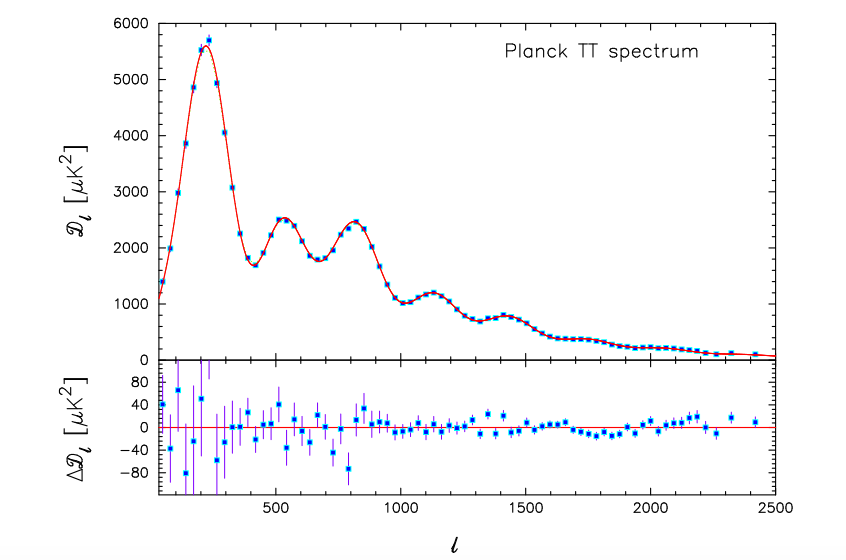
\includegraphics[width=150mm]{Figures/PLANCK_PS_TT}
\caption{Angular correlation power spectrum of the CMB as measured by the Planck experiment. The red line shows the best fit spectrum assuming the $\Lambda$-CDM model. \cite{planck2015}}
\label{fig:powerspectrum} 
\end{figure}


\section{Dark Matter}
There is one piece of the $\Lambda$-CDM puzzle that is conspicuous in its absence from the description so far. Cold Dark Matter (``CDM'' in ``$\Lambda$-CDM'') is one of the key elements of the model. Without a driving force external to the photon-baryon plasma, the baryon acoustic oscillations would decay exponentially. The prominence of the third peak relative to the first and second points to the need for an additional form of matter. This matter would be out of equilibrium with the plasma, and so would collapse into the primordial over-densities, but not experience a restorative pressure. As the baryons oscillate, this ``dark matter'' would continue to accumulate, strengthening the gravitational well. This matter would necessarily couple strongly to neither itself, nor the photons or baryons in the plasma. 


\subsection{Galaxy Clusters}
The evidence for dark matter from the CMB is relatively recent. Astronomers have been chasing the missing matter problem for almost a century. The first conclusive evidence for what is now know as dark matter came from Fritz Zwicky's observations of the velocity distribution of galaxies in the Coma Cluster in 1933\cite{zwicky}, although calculations by Jan Oort of stellar velocities in the Sombrero galaxy hinted that something was amiss a year earlier in 1932\cite{oort}. Assuming that the galactic velocities in the Coma cluster are in a stationary state, the virial theorem can be applied:
\begin{equation}\label{eq:virial1}
\bar{V}=-2\bar{K},
\end{equation}
where $\bar{V}$ is the average total potential energy of the system, and $\bar{K}$ is the average total kinetic energy of the system. Assuming a spherically symmetric system governed by Newtonian gravity, Zwicky then made the following approximations for his calculations:

\begin{equation}\label{eq:potential}
V \approx \frac{-3GM}{5R}
\end{equation}
\begin{equation}\label{eq:kinetic}
K \approx \frac{1}{2}M \bar{\bar{v}}^{2},
\end{equation}
where $M$ is the total mass of the cluster, and $\bar{\bar{v}}$ is the velocity of galaxies in the cluster, averaged over time and mass. Using observations of the doppler shift of the light coming from galaxies within the cluster, Zwicky was able to measure the component of the velocities along the line of sight. He then made the assumption that the velocities are isotropic in order to extrapolate to the overall distribution, $\bar{\bar{v}}=\bar{v}_{LS}$.

Using this method, Zwicky placed a conservative limit of $M > 4.5 \cdot 10^{13}_{\odot}$ on the mass of the Coma cluster. Comparing this result to the amount of light coming from the cluster, he found that the mass-to-light ratio was more than 100 times larger than typical values for local stellar systems. This was the first indication that a large percentage of matter in the universe is not luminous\cite{zwicky}.

\subsection{Galactic Rotation Curves}
Continuing from the early measurements of the spiral galaxies by Jan Oort, it was further observed that the other galaxy types also display strong evidence of containing dark matter\cite{persic}.  A spiral galaxy is well approximated by a flat disk. This makes it possible to measure its galactic rotation curve, or the orbital velocity as a function of radius. Measurements of galactic rotation curves provide some of the most clear and compelling evidence for both the existence and behavior of dark matter on galactic scales.

Measurement's of the luminosity of galaxies show that the density of visible matter tends to decrease exponentially with radius from the galactic center:
\begin{equation}\label{eq:luminosity}
I(R)=I_{0}e^{-R/R_{s}},
\end{equation}
where R is the radius from the galactic center, and $R_{S}$ is the a length scale specific to each galaxy. For the Milky Way $R_{S}$ is about 4 kpc\cite{ryden}. This exponential drop would lead rotation curves proportional to $1/\sqrt{R}$. In contradiction to this, spectroscopic measurements of stars near the galactic center and the H$\alpha$ line outside of the optical radius, show that the rotation curves of spiral galaxies tend to become flat at large radii\cite{rubin, persic}. Beginning with Vera Rubin in 1980 \cite{rubin} and continuing with Massimo Persic and Paolo Salucci \cite{persic} among others, researchers went on to characterize the rotational velocities of spiral galaxies by a ``universal rotation curve'' (URC). 

\begin{figure}[h!]
\centering
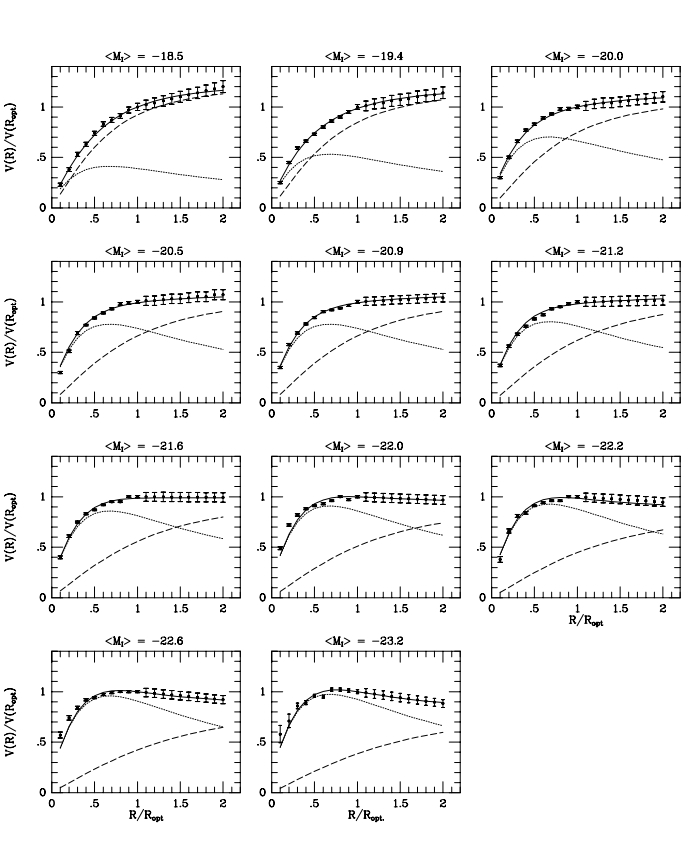
\includegraphics[width=150mm]{Figures/persic_salucci_urc}
\caption{URC (solid lines) fit to average rotation curves surveyed spiral galaxies. The subfigures show bins in luminosity each of which contain about 50 individual rotation curves. Also shown are the contributions from the luminous disk (dotted line) and dark halo (dashed line)\cite{persic}.}
\end{figure}



The URC has two components, one from the luminous, exponentially decreasing disk and the other from a ``dark halo'' which surrounds the galaxy. This dark halo can be thought of as a gas which permeates and surrounds the disk. As a function of $R/R_{opt}$, the mass and velocity contributions from this component are:
\begin{equation}\label{eq:halo_velocity}
V_{d}^{2}=V^{2}(R_{opt})(1-\beta)(1+a^{2}) \frac{x^{2}}{x^{2}+a^{2}},
\end{equation}
\begin{equation}\label{eq:halo_velocity}
M_{h}(x)=G^{-1}V^{2}(1)R_{opt}(1-\beta)(1+a^{2}) \frac{x^{3}}{x^{2}+a^{2}}.
\end{equation}
Both $\beta$, the fraction of disk mass inside of the optical radius, and a, the radius of the halo core are completely determined by the luminosity in this model. The URC fits the observed data very well (on average fitting errors are within 1\%).


More recently, models based on n-body simulations of cold dark matter have become more popular. The most well known of these is the Navarro-Frenk-White (NFW) model. These models produce good fits to high-luminosity galaxies such as the Milky Way, but tend to produce cusps at the galactic center and have trouble replicating the flat cores observed in dwarf galaxies. One solution to this would be a non-zero self-interaction between dark matter particles. It is also possible that this tension could be resolved by gravitational fluctuations, substructure within the halo at the center of these dwarf galaxies, but the ``Cusp-Core'' problem remains an active area of study\cite{weber, navarro}.




\subsection{Modified Neutonian Dynamics}

The agreement between observation of galactic rotation curves and cluster dynamics is quite remarkable, however there is an alternate hypothesis to dark matter that fits the data equally well in many of these cases. Modified Newtonian Dynamics (MOND) postulates that the force of gravity as described by Newton and Einstein is incomplete. In 1983, Milgrom showed that an interpolating function, $\mu$, could be added to Newton's second law to describe the dynamics of galaxies and clusters without the need for dark matter.
\begin{equation}\label{eq:interp_func}
m_{g}\mu(a/a_{0})\vec{a}=\vec{F}
\end{equation}
This interpolating function would be $\approx 1$ at large accelerations, $a\gg a_{0}$, reproducing the classical equation of motion, but would approach $\mu(x)=x$ when $a\ll a_{0}$, where $a_{0}=2 \times 10^{-8} cm\cdot s^{-2}$ is a fundamental constant\cite{milgrom, bekenstein}. 

Following their initial paper in 1983, M. Milgrom and J. Bekenstein reformulated MOND as a classical, lagrangian based field theory, known as AQUAL. In 2004 Bekenstein again reformulated MOND in the context of general relativity. This new tensor-vector-scalar covariant theory is referred to as TeVeS\cite{bekenstein}. 

These theories can produce good fits to galactic rotation data in many cases, but cannot fully describe cluster dynamics without the addition of some dark matter\cite{bekenstein, chaichiana}. Additionally, modified theories of gravity that emulate dark matter have the property that gravitational waves (GW) will travel on different geodesics than photons. In these models, photons will have to travel along a geodesic that mimics the potential well of a dark matter halo, while GW's will not see these imitation potential wells. The recent observation of a neutron star merger has falsified this prediction by showing that gamma rays and GW's travel along nearly identical geodesics. The TeVeS model predicts that the arrival of the gamma ray and GW signals from this event would be about 1,000 days, but the observed delay was only about 2 seconds\cite{teves_false}.



\subsection{Gravitational Lensing}
One of the single most compelling pieces of evidence for dark matter, especially in relation to MOND theories, comes from gravitational lensing data of galactic cluster 1E 0657-56, more commonly known as the bullet cluster. This cluster consists of two subclusters that recently collided and passed through each other. One of these subclusters displays a distinct bow shock that enabled researchers to make a precise measurement of its Mach number, thereby also measuring its velocity. The measured Mach number, $3.2_{-0.6}^{+0.8}$ corresponds to a velocity of $4500_{-800}^{+1100}km/s$\cite{markevitch}. 

During the collision, the gas from the two subclusters would be expected to experience much stronger drag than the stellar matter. This expectation was confirmed by x-ray imaging data from Chandra, which showed that the gas was lagging behind the stars. Further comparison to a mass mapping using gravitational lensing reveals additional matter populations centered near the stellar matter, which are taken to be the dark matter halos of the two subclusters. Fitting a King mass profile ($\rho=\rho_{0}(1+r^{2}/r_{c}^{2})^{-3/2}$) to the lensing data, Markevitch et. al. calculated the density of the dark matter, and limited the self interaction cross section to $\sigma/m < 1 cm^{2} g^{-1}$\cite{markevitch}.

\begin{figure}[h!]
\centering
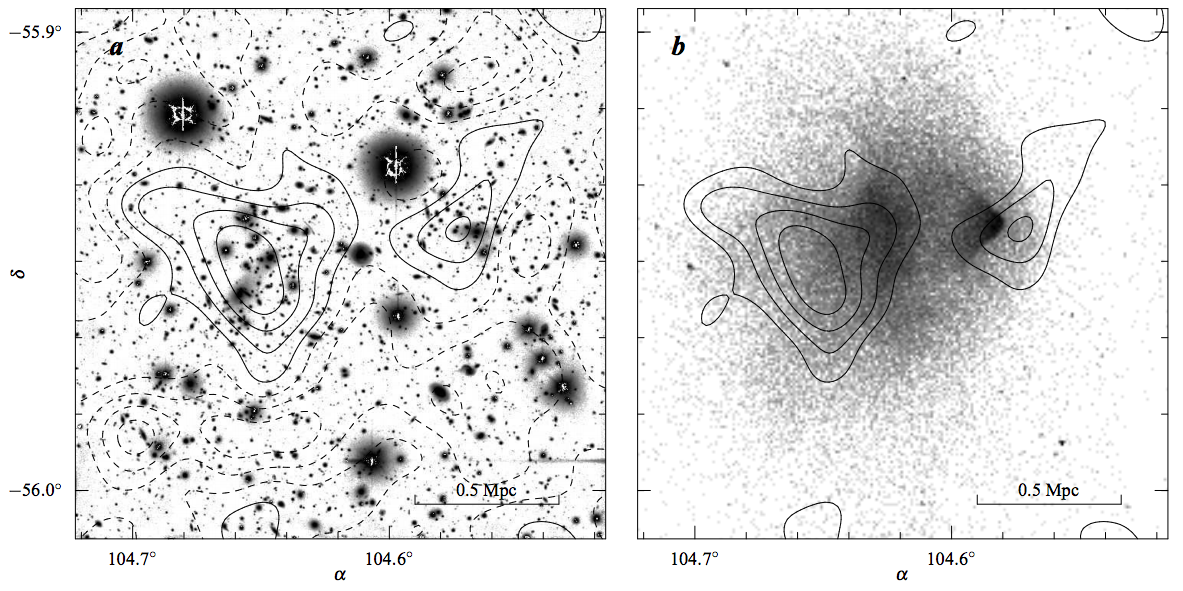
\includegraphics[width=150mm]{Figures/bullet}
\caption{Comparison of the location of dark matter, stellar matter, and x-ray gas in the bullet cluster. The mass density from lensing data, indicated by the solid black lines is imposed over optical (left) and x-ray (right) maps\cite{markevitch}.}
\end{figure}

\section{Dark Matter Candidates}
\subsection{Baryonic Dark Matter}
Now that the existence of cold dark matter has been well motivated, the next step is to investigate what it might be. A reasonable starting point is to look at types of matter that are already known to exist, and ask whether they could exist in high enough abundances to explain the observations of galaxy and cluster dynamics as well as angular correlations in the CMB.  

Within the standard model, the first place to look for dark matter is baryonic matter. It is possible, for instance, that the dark halo is, at least partially, composed of large structures of baryonic material such as brown dwarfs or planets. These massive compact halo objects (MaCHO's) should be observable through gravitational lensing. As a MaCHO passes between an observer on Earth and a background star, the light from that galaxy will be temporarily distorted through gravitational lensing. The EROS-2 experiment conducted a survey of the large Magellanic clouds and found insufficient lensing events to allow MaCHO's as a primary constituent of the Milky Way's dark halo\cite{macho}.

A more general constraint on baryonic dark matter comes from measurements of big bang nucleosynthesis (BBN). BBN refers to the epoch at which the temperature of the universe dropped below the binding energy of deuterium (2.22 MeV). This happened when the universe was about 5 minutes old. During this epoch, the primordial abundances of light nuclei are set as the protons and neutrons are allowed to combine into energetically favored favored states. The ratios of these abundances are highly dependent on $\eta$, the baryon-photon ratio, so the measurement of them, combined with constraints on the photon density from CMB measurements would give a precise value for the baryon density\cite{ryden}. Current measurements of D/H place the baryon density at $\Omega_{b} h^{2} = 0.02202 \pm 0.00046$ \cite{bbn}. This result is within $1\sigma$ of the measurement from the Planck experiment, and taking the reduced Hubble constant to be $h = 0.678$, it indicates that baryons make up only 4.8\% of the energy-density of the universe\cite{planck2015}.


\subsection{Neutrinos}
The remaining candidate for standard model dark matter is the neutrino. Before the CMB decoupled, neutrinos went through a similar process which left the universe filled with neutrinos that had been in thermal equilibrium with the extremely hot and dense early universe. From the annihilation cross-section, the number density of the cosmic neutrino background (CNB) can be calculated to be 3/11 that of CMB photons\cite{ryden},
\begin{equation}
n_{\nu}=3.36 \times 10^{8} \ m^{-3}.
\end{equation}
In order for the CNB to fit the mass density requirement for dark matter, the mass of neutrinos would have to be about $4 \ eV$.\cite{ryden}  Current constraints from Planck show that the combined mass of neutrinos is $< \ 0.23 \ eV$\cite{planck2015}, so neutrinos are not heavy enough to explain the majority  of observed dark matter.


\subsection{Axions}
Currently, the two most well-motivated CDM candidates are Axions and WIMPs. Axions are particularly interesting because they were first theorized as part of a solution to the strong CP problem, and so could simultaneously solve two unsolved problems in physics. Charge-parity (CP) is only conserved by QCD if the vacuum angle, $\theta$, is 0. However,  $\theta$ should be able to take any value, so CP is not predicted to be conserved. Experimental measurements of the neutron electric dipole moment (nEDM) show that CP is, in fact, a good symmetry of QCD. The current limit on nEDM is about $2 \times 10^{-26} \ e \cdot cm$, which in turn limits $\theta$ to $\leq \ 10^{-9}$\cite{nedm,axion_DM}. This unexpectedly small value of $\theta$ points to a tension within QCD. To relieve this tension, R. Peccei and H. Quinn proposed a new spontaneously broken global symmetry, $U_{PQ}(1)$, and showed that if the Higgs potential for at least one quark is invariant under $U_{PQ}(1)$, then $\theta$ is guaranteed to relax to 0. The pseudo-Nambu-Goldstone boson that is associated with the spontaneous breaking of $U_{PQ}(1)$ is known as the axion \cite{peccei_quinn, axion_DM}.

The axion as a candidate for CDM is compelling in that it interacts only very weakly with standard model particles. Axions are expected to be have mass, but be light enough that those produced thermally in the big bang would be too hot to fill the role of CDM. However, populations of axions can be formed non-relativistically in the early universe through vacuum realignment and topological effects in string theory. Axion dark matter created through realignment would be expected to have a mass $m_{a} >6 \ \mu eV$, assuming the initial value of $\theta$ was of order unity. If the initial value of $\theta$ was much smaller than 1, the axion mass could be less than $6 \ \mu eV$\cite{axion_DM}.

Axion searches focus primarily on the tree-level axion-photon coupling, which has the Lagrangian term $\mathcal{L}_{a \gamma \gamma}=g_{a \gamma \gamma}a\mathbf{E \cdot B}$. In the core of a star, the conversion of photons to axions can compete with the production of photons and stream energy away from the core. This would reduce the pressure and causing the the star to compress and heat up, and in so doing, shorten the life of the star. Observations of horizontal branch stars limit the coupling constant for this process to  $g_{a \gamma \gamma}   <10^{-10} GeV^{-1}$, and the excludes axion mass in the range $10^{-3} eV < m_{a} < 2 eV$ \cite{axion_DM, axion_photon}.

In the laboratory, the conversion of axions to photons, and vice versa can be induced in a cavity containing a strong magnetic field. The CAST experiment at CERN used such a cavity to search for axions streaming from the sun. By adding a precisely tuned pressure of helium gas to the cavity, they maximized their sensitivity, and placed a limit of $g_{a \gamma \gamma} \ < \ 2.2 \times 10^{-10} \ GeV^{-1}$ for axions with mass $m_{a} \ < \ 0.4 \ eV$\cite{axion_DM,axion_photon}.
\begin{figure}[h!]
\centering
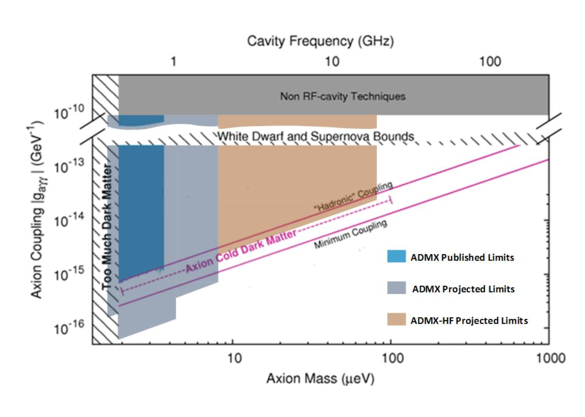
\includegraphics[width=150mm]{Figures/ADMX.png}
\caption{Long term projected limits of the ADMX and ADMX-HF experiments. \cite{ADMX}}
\label{fig:admx} 
\end{figure}

The previously cited limits are on axions that were formed in the cores of stars. These axions, if they existed, would not be able to fill the CDM role. Currently, the only experiment that would be sensitive to dark matter axions is the Axion Dark Matter Experiment (ADMX). This experiment aims to convert axions from the local dark halo into photons using a microwave resonant cavity permeated with a strong magnetic field. In this scenario, a DM axion would interact with a virtual photon from the magnetic field to convert into a real RF photon which can be detected. ADMX and it's sister experiment ADMX-HF are looking for axion dark matter in the mass range $2 \mu eV$ to $100 \mu eV$ and are expected to be able to probe most of the allowable axion CDM phase space\cite{axion_DM,ADMX}.





\subsection{WIMPs}
The other leading candidate for CDM is what is referred to as the Weakly Interacting Massive Particle, or WIMP. ``WIMP'' is a somewhat generic term for a massive particle that couples to standard model particles only through the weak nuclear force. This generic WIMP particle is usually denoted as $\chi$. Many extensions to the standard model, in particular supersymmetric models, include at least one flavor of WIMP. In the very early universe WIMPs will be in equilibrium with the primordial plasma. Just as with CMB photons and CNB neutrinos, once the temperature drops and the universe expands the number and temperature of WIMPs will fall out of equilibrium and the particles remaining will persist as a cosmic relic\cite{susyDM,wimp2}.

When the temperature of the universe is higher than the WIMP mass, $m_{\chi}$ (roughly 10  GeV to 1 TeV) both the WIMP number density, $n_{\chi}$, and temperature will be in thermal equilibrium. Once the temperature drops below the WIMP mass, the number density will fall out of equilibrium and will pick up a Boltzmann suppression factor of $e^{-m_{\chi}/T}$. Once the the scattering rate of cosmic WIMPs drops below expansion rate of the universe, $\chi$ particles will no longer be able to find each other to annihilate, and $n_{\chi}$ will freeze out, becoming the relic density that exists today\cite{wimp2}.

\begin{figure}[h!]
\centering
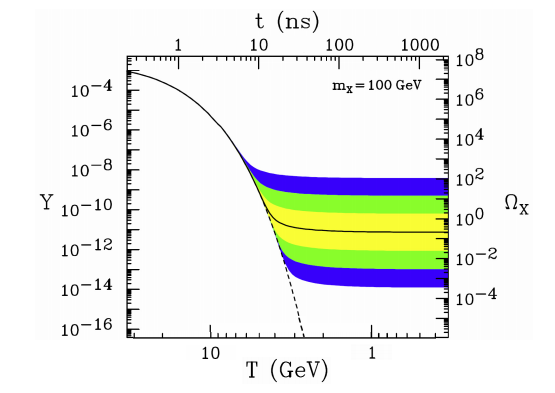
\includegraphics[width=150mm]{Figures/WIMP_relic_density.png}
\caption{WIMP number density in the early universe.The solid line corresponds to the cross section required to account for 100\% of CDM. The colored bands indicate variations by factors of 10, 100 and 1,000\cite{wimp2}.}
\label{fig:reldens} 
\end{figure}


This relic density is determined by the mass of $\chi$, as well as its self-annihilation cross section, $\sigma_{A}$, but is much more strongly dependent upon the cross section.\cite{susyDM,wimp2} If $\sigma_{A}$ is on the scale of the weak force, the density parameter for relic WIMPs will be on the order of what is required for $\Omega_{CDM}$. This is considered one of the most compelling reasons to consider WIMPs as CDM candidates, and has been referred to as the ``WIMP miracle''\cite{wimp1,wimp2, susyDM}.

The creation of the relic density is described by the Boltzmann equation:
\begin{equation}\label{eq:boltz}
\frac{dn_{\chi}}{dt} = -3Hn_{\chi}- \langle \sigma_{A}v \rangle (n_{\chi}^{2}-n_{eq}^{2}).
\end{equation}
In equation \ref{eq:boltz}, the first term on the right hand side is from the expansion of the universe, the $n_{\chi}^{2}$ term is from self annihilation, and the $n_{eq}^{2}$ is the creation of WIMPs from standard model particles.\cite{susyDM,wimp2} The value of $n_{eq}$ is what the number density of WIMPs would be in thermal equilibrium in a static universe. Equation \ref{eq:boltz} has no closed form solution and is solved numerically. There is, however, some insight that can be drawn from some rough analysis\cite{wimp1,wimp2}.

The equilibrium number density for non-relativistic dark matter is given by a simple Boltzmann distribution, $n_{\chi}=g_{\chi}\frac{m_{\chi} T}{2 \pi}e^{-m_{\chi}/T}$.\cite{wimp1} Freeze out will occur when the expansion rate of the universe, $H$, exceeds the annihilation rate of WIMPs, $\Gamma =  n_{\chi} \langle \sigma_{A}v \rangle $. In rough terms, the freeze out temperature can be defined as the temperature at  which $H$ and $\Gamma$ are equal.\cite{wimp1,wimp2}  In the early universe, it is appropriate to make the approximation $H \approx 1.66 g_{*}^{1/2}T^{2}$\cite{susyDM}. In this case the equation $H=\Gamma$ can be rewritten to give the WIMP density at freeze out:

\begin{equation}\label{eq}
n_{\chi,f}
\approx
g_{\chi}\frac{m_{\chi} T_{f}}{2 \pi}e^{-m_{\chi}/T_{f}} 
\approx 
\frac{1.66 g_{*}^{1/2}T_{f}^{2}}{\langle \sigma_{A}v \rangle }
\end{equation}

The ratio of $x_{f} \equiv m_{\chi}/T_{f}$ remains roughly constant between different WIMP models and has a value of about $1/20$. After freeze out, the ratio of $n_{\chi}$ to entropy density, $s$, is constant. In the early universe, $s \approx 0.4 g_{*}T_f^{3}$. Holding $(n_{\chi}/s)$ constant from freeze out to the present day yields the following expression for the current energy density, $n_{\chi,0}$:

\begin{equation}
n_{\chi,0} 
\approx
\frac{1.66 g_{*}^{1/2}T_{f}^{2}}{\langle \sigma_{A}v \rangle }
\cdot
\frac{s_{0}}{0.4 g_{*}T_{f}^{3}}
\end{equation} 

Taking the current entropy density to be $s_{0}=4000 cm^{-3}$\cite{susyDM} yields the following energy density for relic WIMPs:
\begin{equation}
\Omega_{\chi} h^{2}
\approx
\frac{3 \cdot 10^{-27} \ GeV \ cm^{3}}{\langle \sigma_{A}v \rangle}
\end{equation}
Plugging in a typical weak annihilation cross section of about $10^{-25} \ cm^{3} \ s^{-1}$ for $\langle \sigma_{A}v \rangle$ gives $\Omega_{\chi} h^{2} \approx 0.03 \ GeV \ s$ which is close enough to the expected value CDM, $\Omega_{CDM} h^{2} = 0.1188 \ GeV \ s$\cite{planck2015} to make WIMPs an extremely exciting candidate to explain much, if not all, of the non-baryonic dark matter in the universe\cite{susyDM,wimp2}.


\section{WIMP Direct Detection}
The relic density of WIMPs is determined by the cross-section for annihilation into standard model particles, a process which might be observed today by looking for high energy particles coming from high density regions of space such as galactic nuclei. The hypothetical interaction between WIMPs and standard model particles can also be run in two other directions. Production of WIMP dark matter from standard model particles can be searched for using modern particle colliders such as the LHC at CERN, and the scattering of relic dark matter can be probed for using large, low-background detectors. These three methods of detection are referred to as ``indirect detection'', ``production'', and ``direct detection'' respectively. Direct detection is of particular interest because it probes the existing relic dark matter background that is postulated by the $\Lambda$-CDM model.

\begin{figure}[h!]
\centering
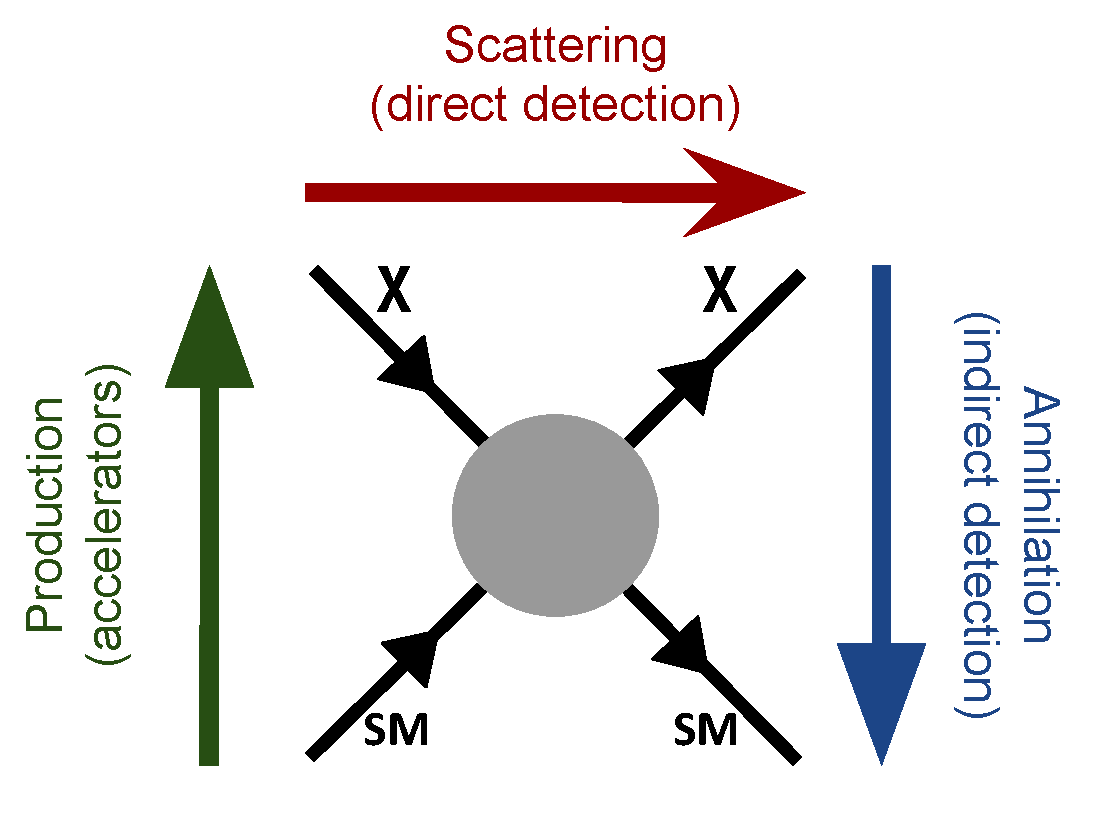
\includegraphics[width=150mm]{Figures/WIMP_interaction.pdf}
\caption{Cartoon of the WIMP-standard model interaction. The green, red, and blue arrows indicate in which direction time is being run for production, scattering, and annihilation, respectively.}
\label{fig:WIMP_SM} 
\end{figure}

\subsection{Cross Section}\label{sec:wimpcrosssection}
The first ingredient needed to calculate the expected interaction rate in a given experiment is the scattering cross section. The WIMP-nucleus scattering cross section will have some dependence on the momentum transfer, $q$, and can be written\cite{dmintro}:
\begin{equation}\label{eq:cross_sec1}
\sigma(q)=\sigma_0F^2(q),
\end{equation}
where $\sigma_0$ is the energy independent, 0-momentum limit of the cross section, and $F(q)$ is an energy dependent form factor. The 0-momentum cross section can be broken into a spin dependent (SD) part and a spin independent (SI) part\cite{wimp_nucleon,dmintro}:
\begin{equation}\label{eq:sisd_cs}
\begin{split}
\sigma_{0,SI}=& \frac{4\mu_A^2}{\pi}[Zf_p+(A-Z)f_n]^2 \\
\sigma_{0,SD}=& \frac{32G_F^2\mu_A^2(J+1)}{\pi J}[a_p\langle S_p \rangle + a_n\langle S_n \rangle ]^2
\end{split}
\end{equation} 
Here, $f_{p,n}$ and $a_{p,n}$ are the SI and SD coupling constants of WIMPs to protons and neutrons, $\mu_A$ is the reduced mass of the interaction, $Z$ is the atomic number, $A$ is the atomic mass, $J$ is the nuclear spin, and $\langle S_{p,n} \rangle$ is the average spin of protons or neutrons in the nucleus. It is typically assumed that $f_p \approx f_n$, so the SI cross section reduces to:
\begin{equation}\label{eq:sics}
\sigma_{0,SI}= \frac{4\mu_A^2}{\pi}f_n^2A^2. 
\end{equation} 

The $\mu_A^2A^2$ dependence in equation \ref{eq:sics} is a result of the non-relativistic nature of the interaction leading the incident WIMP to scatter coherently off of the nucleus as a whole as opposed to the individual nucleons. This is an important result because it indicates a large benefit to using heavy nuclei as experimental target media. For instance, a detector which uses xenon as its target medium (A$\approx$131) will be over 10 times more sensitive to a 100 GeV WIMP than an argon based detector (A$\approx$40) with the same mass of target material. 

Another important result is that the SD cross section does not have the same $\mu_A^2A^2$ dependence. In many nuclei, the nucleon spins, and therefore the SD cross sections, cancel entirely. In the case of xenon, the only isotopes that have non-zero spin and a non-negligible natural abundance are $^{131}$Xe (J=3/2) and $^{129}$Xe (J=1/2), which together make up just under half of the natural xenon abundance. Since xenon has an even number of protons, $\langle S_p \rangle$ is very close to zero (-0.009 for $^{131}$Xe and 0.028 for $^{129}$Xe). The neutron part of the SD cross section in $^{129}$Xe and $^{131}$Xe is about 2,000 and 400 times that of a single-neutron, respectively\cite{dmintro}. We can compare this to the SI cross section of xenon, which is $>5\times 10^7$ times larger than the single-nucleon cross section for a 100 GeV/c$^2$ WIMP. This suppression of the SD cross section in comparison with the SI cross section has led to much less stringent limits on spin independent interactions than on spin dependent interactions as can be seen in the results from the LUX detector in figure \ref{fig:wimplimits}.
\begin{figure*}
        \centering
        \begin{subfigure}[b]{0.475\textwidth}
            \centering
            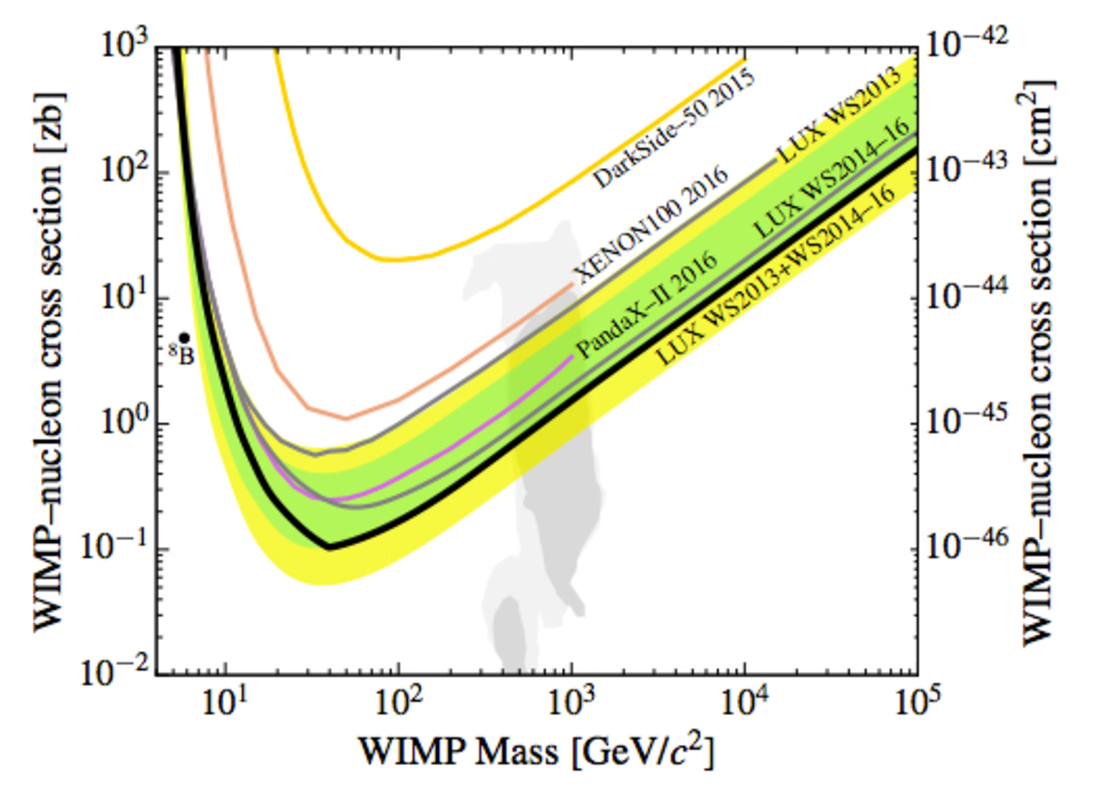
\includegraphics[width=\textwidth]{Figures/WIMP_nucleon.pdf}
            \caption{} 
            \label{fig:wimplimits_si}
        \end{subfigure}
        \hfill
        \vskip\baselineskip
        \begin{subfigure}[b]{0.475\textwidth}   
            \centering 
            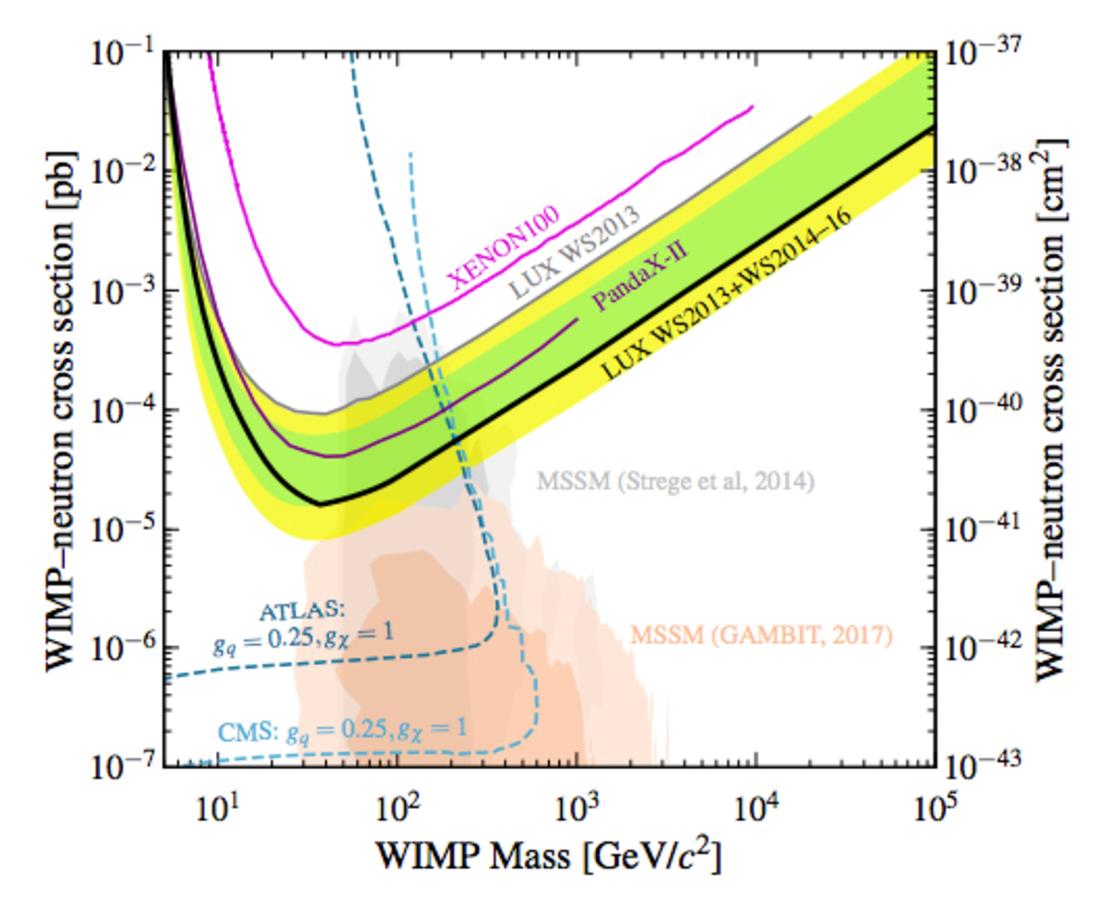
\includegraphics[width=\textwidth]{Figures/WIMP_neutron.pdf}
            \caption{}   
            \label{fig:wimplimits_sdn}
        \end{subfigure}
        \quad
        \begin{subfigure}[b]{0.475\textwidth}   
            \centering 
            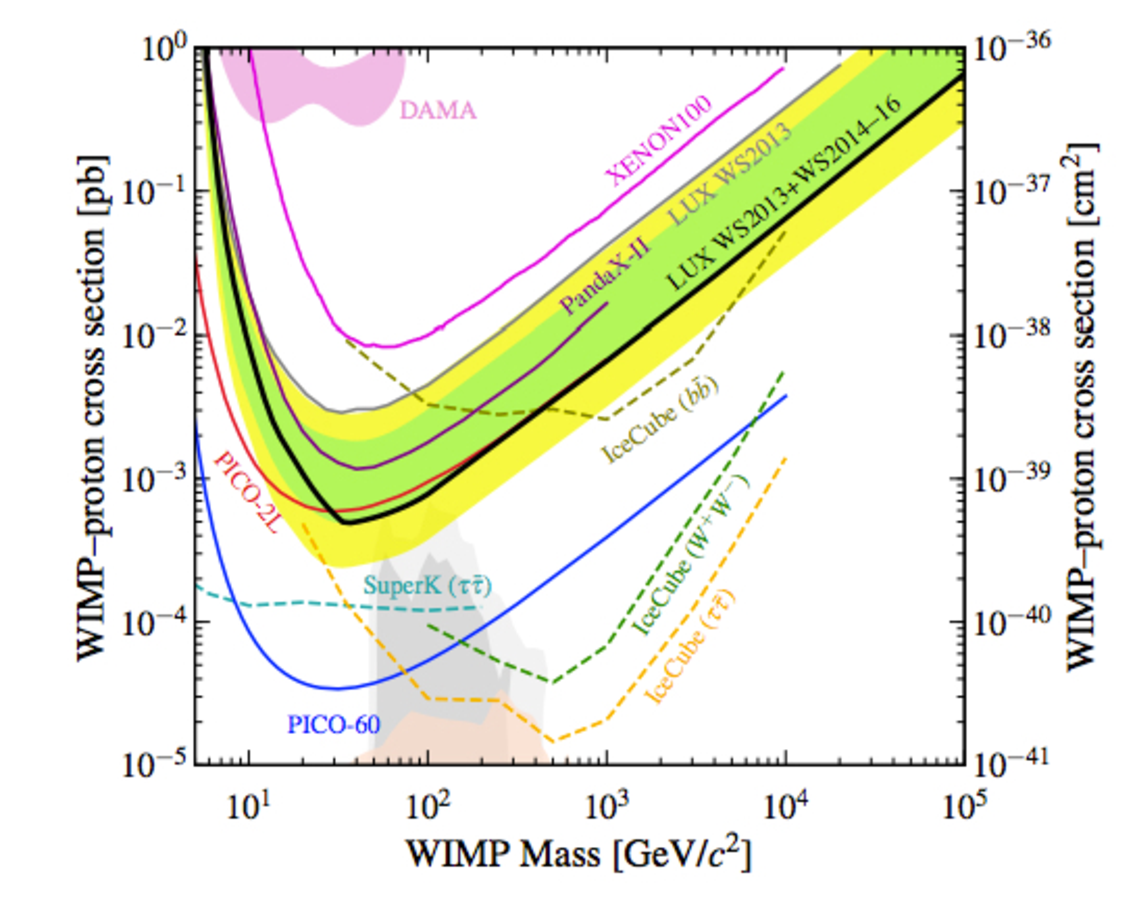
\includegraphics[width=\textwidth]{Figures/WIMP_proton.pdf}
            \caption{}
            \label{fig:wimplimits_sdp}
        \end{subfigure}
        \caption{Limits on the SI single-nucleon (a), SD single neutron (b), and SD single proton (c) cross sections. This limits were take from the LUX experiment's full exposure (332 days). The SI limit is roughly 5 orders of magnitude better than the SD neutron limit, which itself is about 2 orders of magnitude better than the SD proton limit. The solid black lines show the experimentally measured limits, and the green and yellow regions show the 1- and 2-$\sigma$ expectations. Figures were taken from \cite{lux_2017} and \cite{lux_sd}.}
        \label{fig:wimplimits}
    \end{figure*}

\subsection{Recoil spectrum}
The WIMP halo is expected to have only a small amount of bulk rotation; that is it is expected to be more akin to a gravitationally bound ideal gas than an accretion disk. The velocities of WIMPs in such a halo roughly modelled by a Maxwellian distribution\cite{dmintro}:
\begin{equation}\label{eq:veldist}
f(\vec{v}_{halo})= e^{-v_{halo}^2/v_0^2}/k,
\end{equation}
with $v_0=220\pm 20$ km/s being the local circular velocity around the galactic center and $k$ being a normalization constant. In the lab frame the observed velocity of an incident WIMP will be $\vec{v}_i=\vec{v}_E+\vec{v}_{halo}$. Here, $\vec{v}_E$ is the velocity of the earth with respect to the galaxy which is the sum of $\vec{v}_0$, the sun's peculiar velocity, $\vec{v}_s$, and the orbital velocity of the earth around the sun, $\vec{u}_E(t)$\cite{dmvelocity,dmintro}:
\begin{equation}
\vec{v}_E(t)=\vec{v}_0+\vec{v}_{sun}+\vec{u}_E(t).
\end{equation}
The contribution  to $\vec{v}_E(t)$ from the velocity of the sun with respect to the galactic center ($|\vec{v}_0+\vec{v}_{sun}|$) is about 232 km/s, and $\vec{u}_E(t)$ acts to add a 6\% annual modulation. This modulation would presumably introduce a detectable effect in the scattering rate of WIMPs. The DAMA/LIBRA NaI scintillation detector\cite{dama} has observed with 9.3-$\sigma$ confidence annual modulation in their 2-6 keV, single-scatter event rate. This result, however, is in significant tension with other experimental limits (see for instance figure \ref{fig:wimplimits_sdp}).

We can use this velocity distribution to write the scattering rate as a function incident velocity, $v_i$. This will give the total number of WIMP-nucleus scattering events per unit time per gram of material with atomic weight, $A$:
\begin{equation}
dR(v_i)=\frac{N_A}{A}n_{\chi}f(\vec{v}_i-\vec{v}_E)\sigma v_i d^3\vec{v}_i,
\end{equation}
with $N_A$ being Avagadro's number and $n_{\chi}$ being the local number density of WIMPS.

The velocity of a WIMP in the lab frame is highly non-relativistic. This being the case, collisions between WIMPs and the target nuclei of earth-bound detectors can be well modeled by classical elastic scattering. The recoil energy, $E_R$, for elastic scattering of a non-relativistic WIMP of mass $M_{\chi}$ off of a nucleus of mass $M_A$ is given by\cite{dmintro}:
\begin{equation}\label{eq:recoilE}
E_R=\frac{E_ir}{2}[1-cos(\theta)],
\end{equation}
where $E_i=\frac{1}{2}M_{\chi}v_i^2$ is the energy of the incident WIMP, $\theta$ is the recoil angle, and $r=4M_{\chi}M_{A}/(M_{\chi}+M_{A})^2$ is a kinematic factor. 

For a WIMP with a given $v_i$, the nuclear recoil energy will be even distributed between 0 and $E_ir$. These uniform distributions can then be weighted by $dR(v_i)$ and then integrated over $v_i$ to give the total differential scattering rate:
\begin{equation} \label{eq:recoilspec1}
\frac{dR}{dE_{r}}=\int_{E_{min}}^{E_{max}}dR(v_i)/E_ir
\end{equation}
For the limits of integration we could take into account the escape velocity of the galaxy, but setting $E_{max}=\infty$ yields a good approximation and makes evaluation of the integral simpler. Only WIMPs with incident energy equal to or greater than $E_R/r$ will contribute to the scattering rate at $E_R$, so we will set $E_{min}=E_R/r$. Under this approximation, the normalization constant in equation \ref{eq:veldist} becomes $k=(\pi v_0^2)^{3/2}$. If we make the further assumption that $\vec{v}_E=0$, we can write:
\begin{equation}
\begin{split}
dR(v_i)=&\frac{R_0}{2\pi v_0^4} e^{-v_i^2/v_0^2}v_i (4\pi v_i^2dv_i)\\
=&\frac{2R_0}{v_0^4} e^{-v_i^2/v_0^2}v_i^3dv_i
\end{split}
\end{equation}
where, 
\begin{equation}
R_0=\frac{2N_A}{\sqrt{\pi}A}n_{\chi}\sigma_0 v_0,
\end{equation}
for constant cross section. Equation \ref{eq:recoilspec1} then becomes:
\begin{equation} \label{eq:recoilspec2}
\frac{dR}{dE_{r}}= \frac{R_0}{E_0 r}\frac{2}{v_0^2} \int_{E_R/r}^{\infty}   e^{-v_i^2/v_0^2}v_idv_i.
\end{equation}
If we make a change of variables to energy space, this integral becomes:
\begin{equation} \label{eq:recoilspec3}
\frac{dR}{dE_{r}}= \frac{R_0}{E_0 r} \int_{E_R/r}^{\infty}   e^{-E_i/E_0}dE_i,
\end{equation}
which easily evaluates to:
\begin{equation} \label{eq:recoilspec4}
\frac{dR}{dE_{r}}=\frac{R_{0}}{E_{0}r}e^{-E_{r}/E_{0}r}
\end{equation}
Here we see that $R_0$ will give the total scattering rate.

\begin{figure}[h!]
\centering
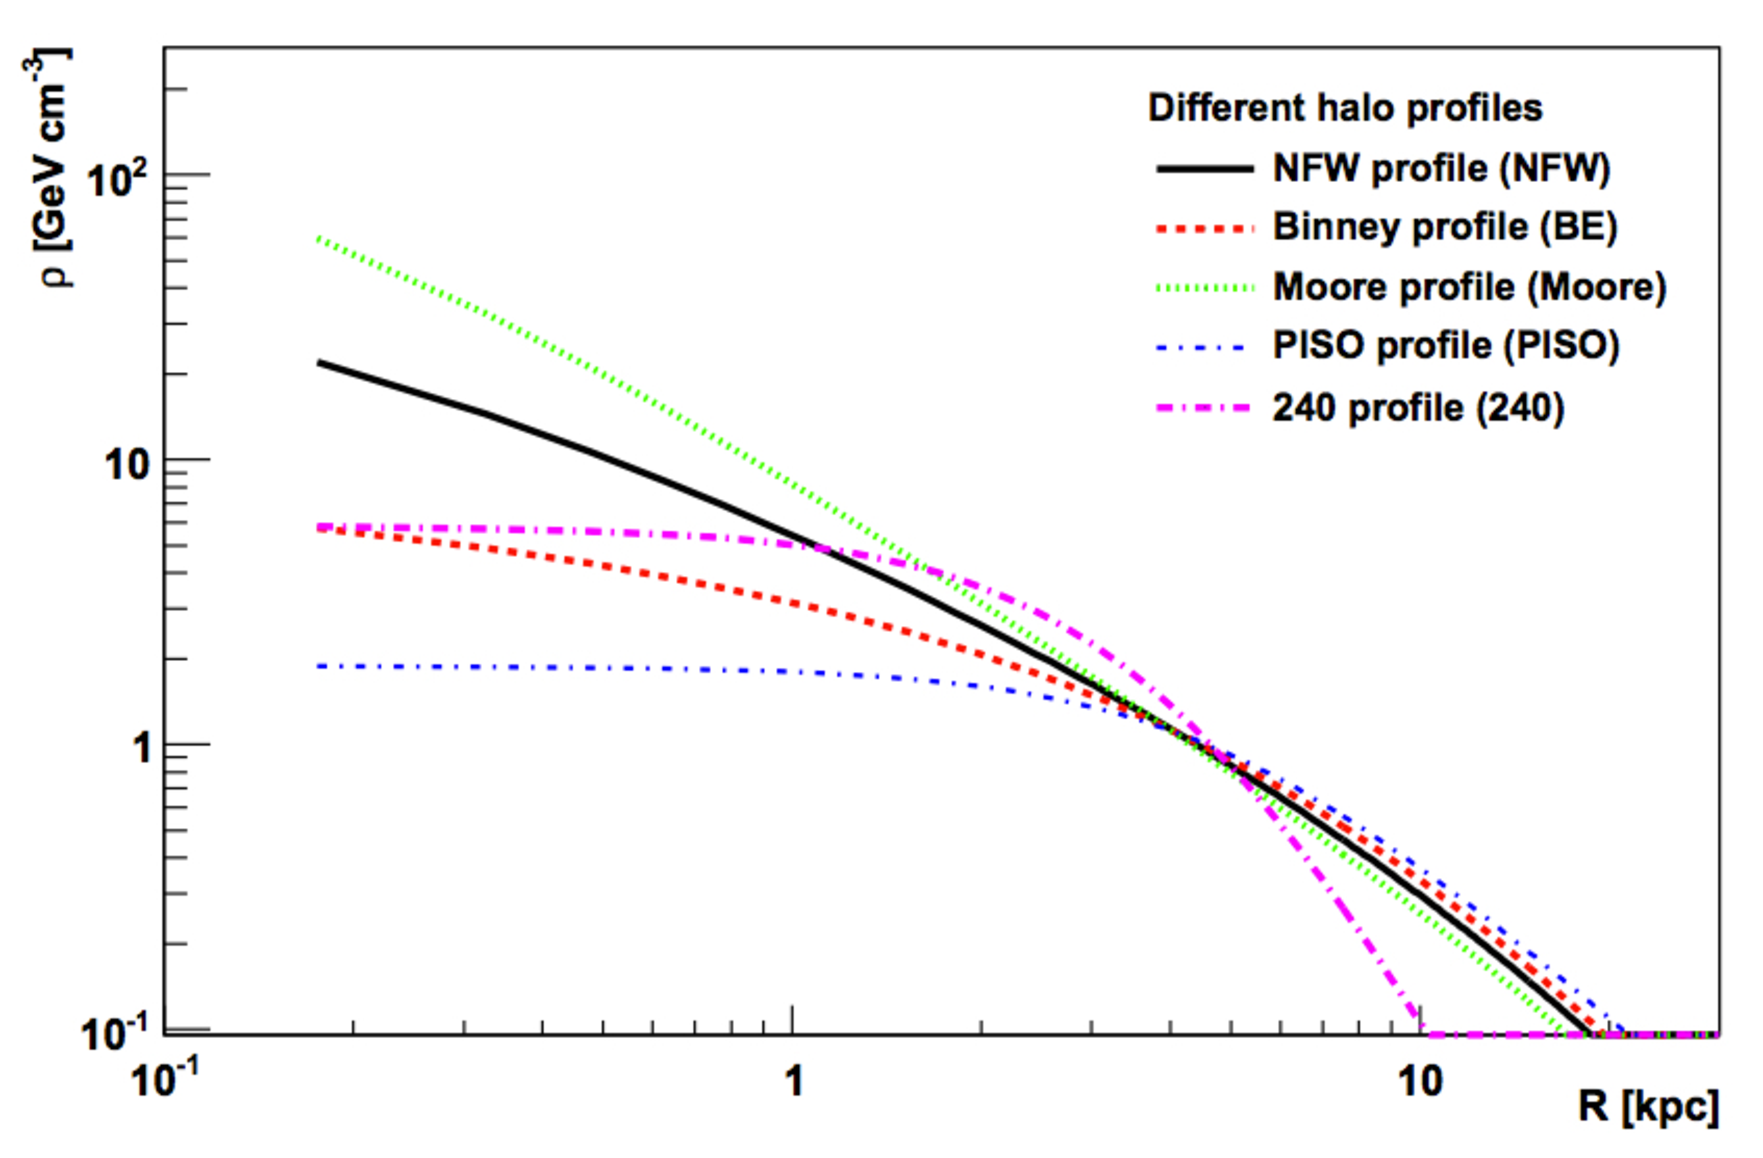
\includegraphics[width=150mm]{Figures/DMprofiles.pdf}
\caption{Various theoretical halo profiles. The sun is at about 8 kpc. The significant variance of $\rho_{\chi}$ for the different models limits the accuracy of scattering rate estimates for direct detection experiments. Figure from \cite{weber}.}
\label{fig:WIMPprofiles} 
\end{figure}
From measurements of the rotation curve of the Milky Way, the local dark matter density is expected to be approximately 0.2-0.4 GeV cm$^{-3}$. This value is highly dependent on theoretical profile model and could be as high as 0.7 GeV cm$^{-3}$ given a nonuniform halo density\cite{weber}. Here we assume a middling value of 0.3 GeV cm$^{-3}$. If we take $M_{\chi}$ 100 GeV/c$^2$, and $M_A$=122 GeV/c$^2$ (xenon atomic mass), we have $r=0.99$ and $E_0=27$ keV. In this case the total scattering rate in counts$\cdot$ day$^{-1}\cdot$kg$^{-1}$ will be:
\begin{equation}
\begin{split}
R_0=& \frac{2}{\sqrt{\pi}}\frac{(1000 \text{\ g/kg})\times (6.022\times 10^{23}\text{\ atoms/mole})}{131 \text{\ g/mole}}\frac{0.3 \text{\ GeV/cc}}{100 \text{\ GeV}/c^2}\sigma_0 (7.34 \times 10^{-4}c)\\
\approx&\left( \frac{131}{A} \right)\left( \frac{\sigma_0}{1 \text{\ pb}} \right)(0.3 \text{\ counts/kg/day}).
\end{split}
\end{equation}
So for a xenon detector and a WIMP-nucleus cross section of 1 picobarn, there would be about one event every 33 days per kilogram of detector material.

The effect of the finite galactic escape velocity, $V_{esc}=540$ km/s, can me approximated by introducing a cutoff to equation \ref{eq:recoilspec4}. Very nearly all of the WIMPs with velocity greater than $V_{esc}$ should have left the halo, so maximum recoil energy will be $E_{max}=\frac{r}{2}M_{\chi}v_{esc}^2$. For xenon detectors:
\begin{equation}
E_{max}=\frac{1}{(1+M_A/M_{\chi})^2}(790 \text{\ keV}).
\end{equation}
Detectors which have energy thresholds greater than $E_{max}$ will be completely insensitive to WIMPS of that mass. In addition to the hard cut off at $E_{esc}r$, the exponential nature of equation \ref{eq:recoilspec4} means that detectors will be significantly less sensitive to WIMPs for $E_0r<E_{threshold}$. For xenon:
\begin{equation}
E_{0}r=\frac{1}{(1+M_A/M_{\chi})^2}(131 \text{\ keV}).
\end{equation}
This means that a xenon detector with a 20 keV threshold will begin to lose sensitivity for $M_{\chi}<20$ GeV$/c^2$, and will be completely insensitive to WIMPs with $M_{\chi}<3$ GeV/$c^2$. This places a large incentive for direct detection experiments to have a very low threshold.

\begin{figure}[h!]
\centering
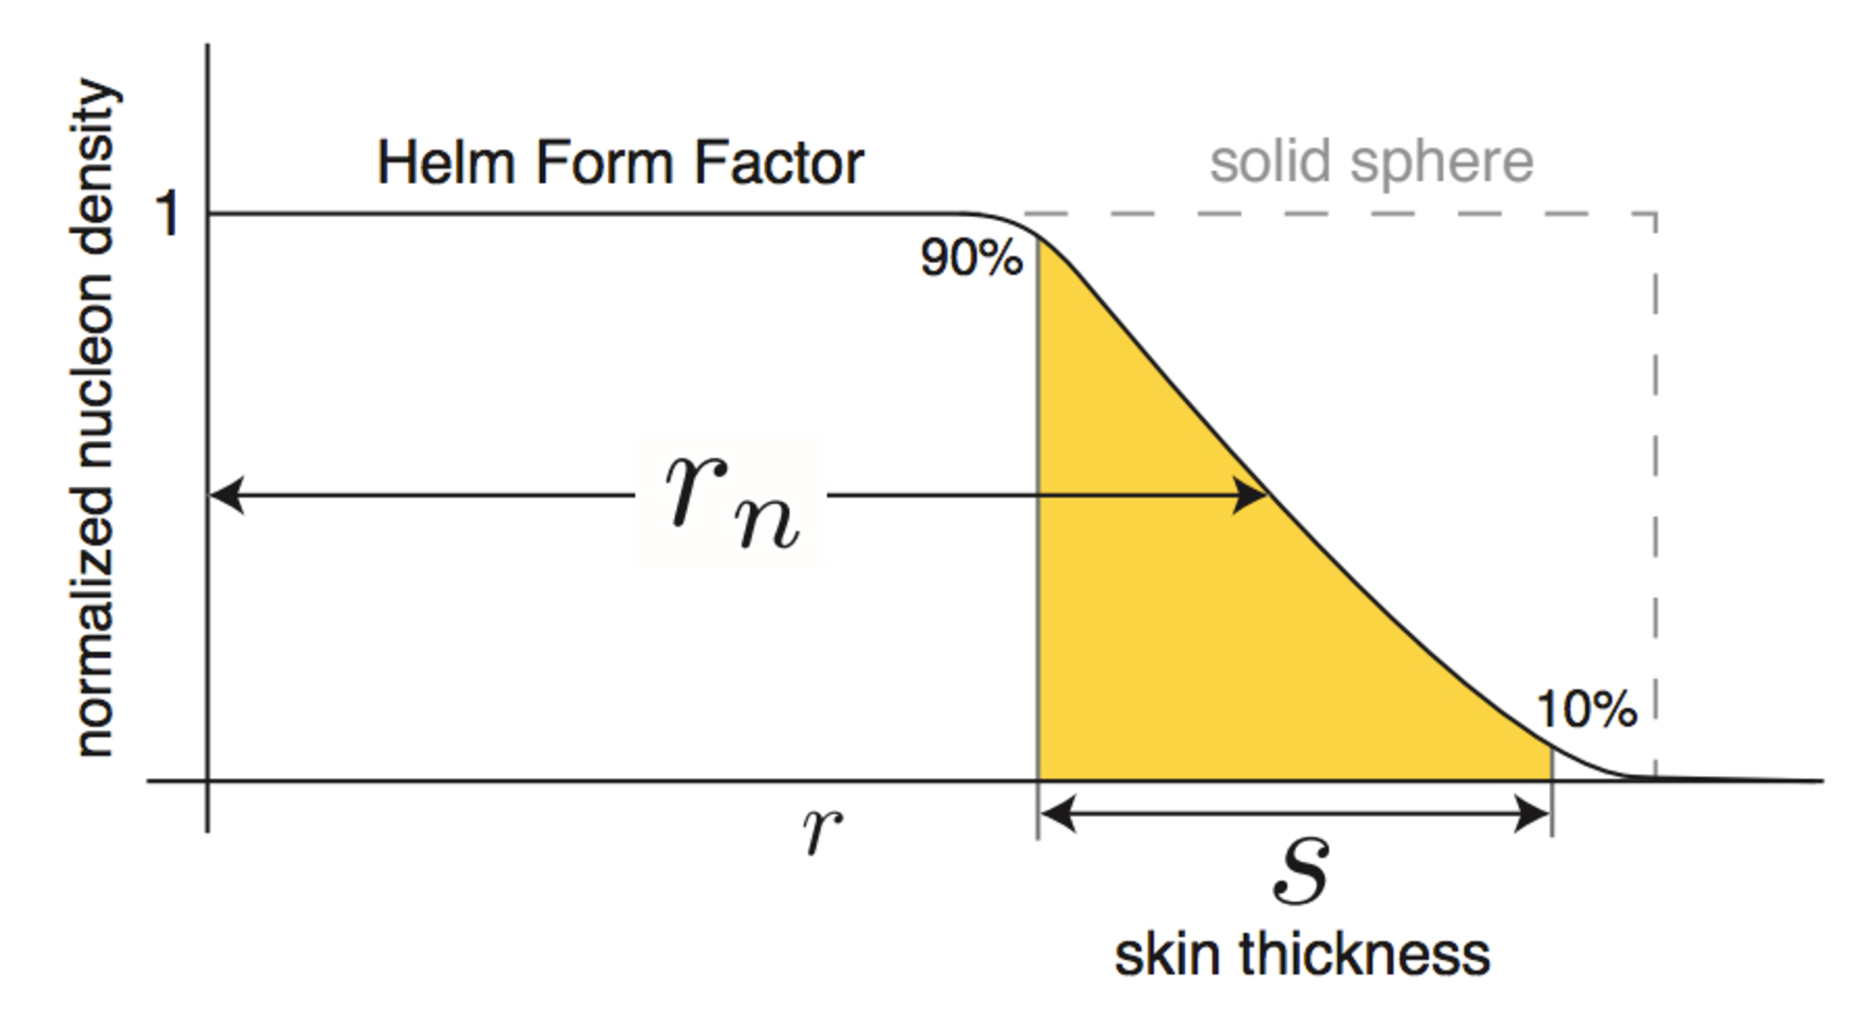
\includegraphics[width=150mm]{Figures/helm.pdf}
\caption{Helm approximation of the nucleon density. This approximation has the form of a solid sphere with a Gaussian falloff of thickness, S. Figure from \cite{carlos}.}
\label{fig:helm} 
\end{figure}
In the derivation of equation \ref{eq:recoilspec4}, we assumed a constant scattering cross section. This, however, neglects the nuclear form factor, $F(q)$, which was introduced in equation \ref{eq:cross_sec1}. This form factor takes into account the nuclear wave-function, which becomes important at higher momentum transfers where coherent scattering begins to break down. Under the Born approximation and for spherically symmetric nucleon density, $\rho{r}$, the form factor is:
\begin{equation}\label{eq:scatformfac1}
F(q)=\frac{4\pi}{q}\int \rho(r)\sin(qr)rdr.
\end{equation}
The most common approximation for the nucleon distribution the Helm approximation- a solid sphere which convolved with gaussian to create a smooth fall off at the edge\cite{helm}. Plugging this into equation \ref{eq:scatformfac1} yields:
\begin{equation}\label{eq:scatformfac2}
F(q)=\frac{3[\sin(qr_n)-qr_n\cos(qr_n)]}{(qr_n)^3}e^{-(qs)^2/2},
\end{equation}
where $r_n$ is the nuclear radius and the skin width, $s$, is the width of the Gaussian fall off in the Helm approximation. The skin width is usually taken to be $s=0.9$ fm\cite{Lewin}, and the nuclear radius can be approximated $r_n\approx 1.14 A^{1/3}$.

When the de Broglie wavelength, $h/q$, becomes comparable to the nuclear radius, $r_n$, coherent scattering will break down. This causes a drastic fall in the scattering rate. Xenon, for instance, will lose coherence at about 100 keV, while smaller elements will maintain the benefit of coherent scattering to significantly higher energies. This effect will compete against benefit from the $A^2$ dependence of $\sigma_{0,SI}$. Ultimately the low-momentum benefit of xenon as a target medium, together with self-shielding effects which will be described later, makes xenon the most popular and promising target material for direct detection experiments.
\begin{figure}[h!]
\centering
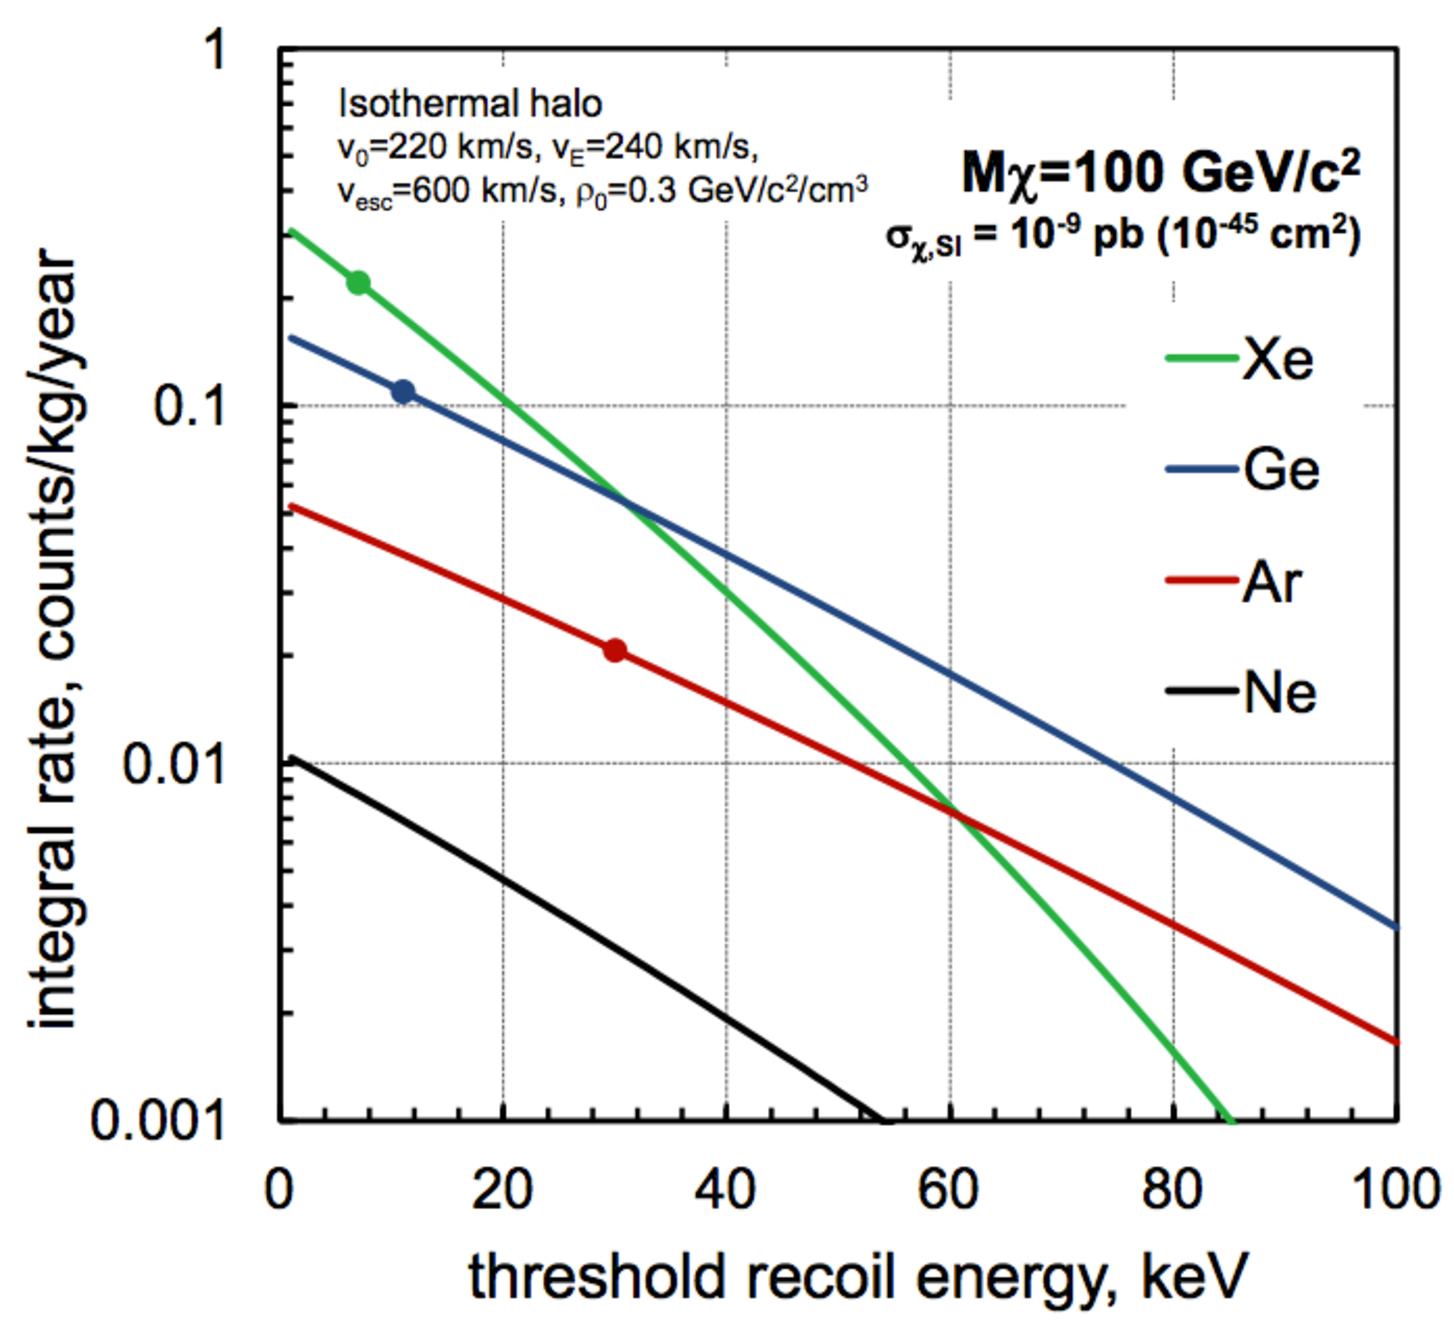
\includegraphics[width=150mm]{Figures/recoil_spec.pdf}
\caption{WIMP scattering rate as a function of energy taking into account the nuclear form factor. Xenon's large size is a double edge sword. At low energy, the $A^2$ dependence of $\sigma_{0,SI}$ wins out and xenon has a significant advantage over competing media. At large momentum transfers, however, decoherence dominates, forcing xenon to fall much more quickly than argon, neon, or germanium. Figure from \cite{henrique}.}
\label{fig:helm} 
\end{figure}




\section{Thesis Outline}
In this chapter, we discussed the evidence for particulate cold dark matter in general. We then discussed the motivation and proposed detection techniques for Weakly interacting massive particles (WIMPS). In the next chapter, we will continue to narrow our focus to liquid xenon time projection chambers as WIMP detectors. This will include a discussion of the microphysics behind energy deposits in liquid xenon, as well as the design, construction, and operation of the LUX and LZ dark matter detectors.

In chapter 3 we will discuss a technique for monitoring the purity of liquid xenon. We have improved on an existing technique using novel methods of optimization. We detail the empirical studies that went into this optimization, as well as the theoretical motivation behind them.

Chapter 4 will describe the LUX post-run04 calibration campaign. There are several internal sources novel to the LUX detector which were injected during this timeframe. We will catalog these sources, and present signal corrections derived from them. We will also describe a systematic pathology in the charge signals, as well as our attempt to account for it. 

Finally, chapter 5 will describe in detail the results from the novel $^{14}$C injection that occurred during the post run04 injection campaign. We will derive charge and light yields, as well as recombination fluctuations from energies ranging from 5-140 keV. We will also present a comparison to the theoretical spectrum.



\chapter{Liquid Xenon Dark Matter Detectors}\label{chap:2}
The LUX detector and its upcoming successor, the LUX-ZEPLIN (LZ) detector, have been on the cutting edge of direct detection limits for almost a decade. These are examples of two-phase xenon time-projection chambers (TPC's). The strongest current limits on WIMP mass and scattering cross-section are placed by measurements using this specific type of detector. In this chapter we will examine what makes xenon as a detector medium so attractive. We will present on the design and operation of LUX, and will develop tools needed to model interactions within the detector.

\section{Xenon as a Detector Medium}
\subsection{Noble Gasses}
Noble gasses are chemically inert, which gives them several properties that make them exciting candidates as WIMP detection media. An interaction of an energetic particle with a target atom will transfer some or all of the particle's energy to the target material. This transferred energy is divided into three channels: scintillation light, free charge, and heat. In a noble gas, the light subsequent to the excitation of an atom will be generated at a wavelength to which the gas is transparent. This scintillation light can therefore be collected and measured.

A noble gas detector will also be sensitive to the charge channel. Free electrons within the medium can be long-lived ($>$1ms), assuming the gas has been purified of more chemically active contaminants. This gives experimenters the chance to extract the free electrons created by an interaction. Since the noble elements are inert, it is also fairly easy to remove problematic impurities by chemical means such as a heated zirconium getter, as used by LUX and LZ.

Typically, detectors that use a noble element as a target have access to one or both of these two channels: charge and light. It is difficult to measure a heat deposit in a liquid or gas-phase detector, but it has been suggested that it may possible to gain access to this channel using a bubble chamber\cite{bubble}. Alternatively, cryogenic solid state experiments are able to measure phonons from interactions. The SuperCDMS experiment, for instance, uses a set of silicon and germanium detectors cooled to 30 mili-Kelvin as its target material\cite{cdms}. Heat-detectors tend to outperform charge and light detectors at low-WIMP masses, because in this regime the charge and light signals start to drop below their respective thresholds.

The relative amount of energy measured in the three channels can be used to help determine whether the interaction of the inclement particle with the xenon atom was an electronic recoil (ER) where the particle scattered with an orbital electron, or a nuclear recoil (NR) in which it scattered with the nucleus. This determination allows for strong background rejection, since most low-energy backgrounds are $\beta$'s and $\gamma$'s, which only scatter electronically, while WIMP's, which interact via the weak force, will scatter off of the nucleus. Access to the heat channel would provide greatly improved discrimination between ER events, in which nearly all of the energy is initially divided between charge and light, and NR events, in which a comparatively large portion of the energy goes into heat.

The most common noble elements used in WIMP detection experiments are argon and xenon. Neon has also been used in the DEAP/CLEAN collaboration\cite{clean1,clean2}. Guo and McKinsey also propose the use of superfluid helium\cite{he_dm}. The lighter noble gasses, helium and neon, are complimentary to experiments that use argon or xenon because they are more sensitive to low-mass WIMPs ($<$ 10 GeV), whose interactions with the heavier elements would be kinematically suppressed.

\subsection{Xenon Density}
Xenon is perhaps the most exciting candidate of the noble gasses, in part because it is the heaviest stable noble element. It has, on average, 131.3 nucleons in its nucleus, and at its triple point, has a liquid density of 2.978 g/cc. This is higher than the density of aluminum. As was shown in section \ref{sec:wimpcrosssection}, the scattering cross section of a WIMP with an atom with $A$ nucleons is proportional to $A^2$, so a larger atom typically means a better sensitivity. 

The high density also has its own benefit, independent of the scattering cross section. Low-energy electronic backgrounds, such as $\gamma'$s and $\beta$'s, will generally be stopped within a centimeter in the liquid xenon. External backgrounds, and those generated on the detector walls will therefore be highly suppressed at the center of the detector. This is referred to as ``self-shielding'', and allows for greatly improved background discrimination. A detector that can reconstruct to location at which an event occurred will be able to fiducialize its volume, assigning more weight to an event near the center of the detector than one near the wall. A simple version of this would be to define some subset of the detector as a ``fiducial volume'', and apply a strict cut, rejecting any event that occurs outside of the fiducial region and accepting any event that occurs within it.
\begin{figure}[h!]
\centering
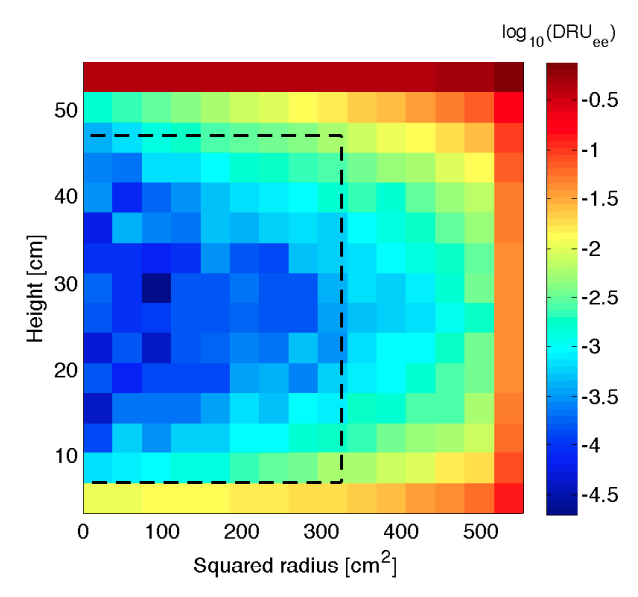
\includegraphics[width=\linewidth]{Figures/lux_fiducial.png}
\caption{Simulated electronic backgrounds in the LUX detector, from 0.9 to 5.3 keV. The black outline shows the 118 kg fiducial which was used to analyze the Run03 data.\cite{lux_fiducial}}
\label{fig:lux_fiducial} 
\end{figure}

\clearpage
\subsection{Radiopurity}
In order for the self-shielding to be effective, the xenon must be free of any dissolved radioactive impurity, and must itself not have any long-lived radioactive isotopes. There are several cosmogenically activated xenon isotopes, but these all have a half life of less than two weeks. They will therefore be suppressed by long-term storage of the xenon underground.

Krypton, for instance, would not be a good candidate for a detector material because it has a relatively large atmospheric abundance of the radioactive isotope $^{85}$Kr, roughly 20 parts per trillion ($^{85}$Kr/$^{nat}$Kr). In fact, for xenon to be used as a WIMP target material, it must first be meticulously cleansed of even trace amounts of krypton. Krypton-85 undergoes a beta-decay with a Q-value of 687 keV and a half life of 10.8 years. It is sourced into the atmosphere by anthropogenic fission to a specific activity of about 1 Bq per cubic meter of air. 

In order to hold the krypton-85 activity below the average expected background rate, the LUX goal was to limit the krypton concentration to less than 5 parts per trillion (grams $^{nat}$Kr per gram Xe). This corresponds to about 700 atoms of $^{85}$Kr per kilogram of xenon, or an activity of about 2$\times \ 10^{-3}$ events/day per kg of xenon per keV. LZ plans to have over 150 times the exposure that LUX had, so in order to keep the number of krypton-85 events constant, it has set a goal of 0.015 parts per trillion\cite{lz_tdr}. 

As mentioned previously, it can be difficult to separate noble gasses from each other. The fact that they are inert means that chemical means are a non-starter. The removal of krypton from xenon is typically done using mass-sorting techniques, such as distillation or mass chromatography. LUX and LZ rely on the latter technique, which has been demonstrated to be effective down to at least 200 ppq (0.2 ppt)\cite{lz_tdr,lux_krremoval}.

Since the required decay rate of $^{85}$Kr is so low, a factor of 10 or even 100 times increase over the concentration limit would not be obvious in the data until weeks or months had passed. It would then take on the order of a year to reprocess the xenon and try again. It is therefore important to have in-situ measurements of the krypton concentration at every step of the construction and operation of a xenon dark matter experiment. Typical mass-spectrometers can only detect concentrations down to about 1 part per million, which is six orders of magnitude too high. LUX and LZ use a technique that was initially developed by Leonard et. al., which augments commercially available mass spectrometers to allow for detection of trace gasses in xenon down to $<$1 ppt\cite{sampling_doug}. In chapter \ref{chap:sampling}, we present methods to improve this technique in order to achieve sensitivities down to the order of 1 ppq. 

There is also an atmospheric component of the radioactive $^{39}$Ar isotope that must be removed from the xenon before it can be used as an effective WIMP detection medium. This isotope has a lower activity in the atmosphere than does $^{85}$Kr. Additionally, because argon is more different in mass from xenon than krypton is, techniques used to detect and remove krypton from xenon will simultaneously and more effectively detect and remove argon.

\section{The LUX Detector}
\subsection{Overview}
LUX and its successor, LZ, are examples of dual-phase, gas/liquid xenon time projection chambers (TPC). TPC's in general can provide a 3D reconstruction of the event position, allowing the internal volume to be fiducialized in order to exploit xenon's self-shielding properties. Specifically, a two phase detector is well suited for WIMP detection, because it produces an amplified charge signal. 

LUX was located in the Davis cavern at the Sanford Underground Research Facility in Lead, South Dakota. It is 4850 feet underground (4300 m w.e.) in order to shield it from cosmic rays. The detector itself was immersed in a large water tank to further shield it from neutrons and gammas. LUX contained about 370 kg of xenon and used a fiducial volume containing about 118 kg as its WIMP target. The remaining xenon acts as a shield from external gammas and betas. The LZ detector will be installed in the same water tank in the Davis cavern, and is slated to have about 20 times the total active xenon mass (7,000 kg) and nearly 50 times the fiducial mass (5,600 kg).
\begin{figure}[h!]
\centering
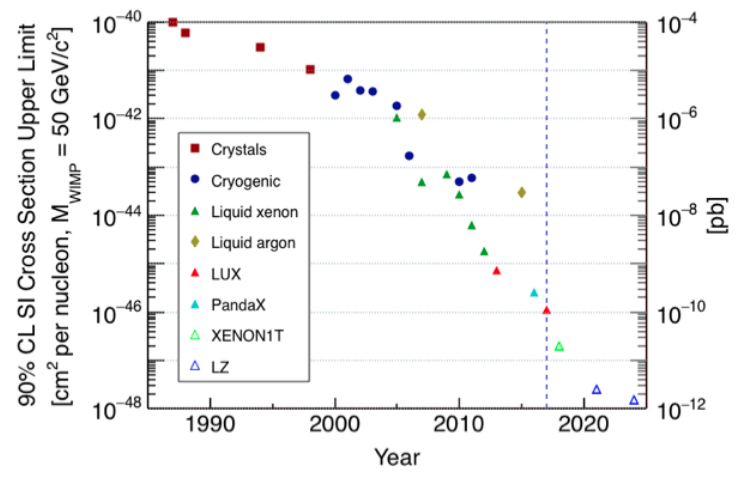
\includegraphics[width=\linewidth]{Figures/limits_trend.png}
\caption{Experimental limits on spin-independent WIMP-nucleon cross section. Figure taken from \cite{lz_tdr}. The open points represent projected limits. The XENON-1T preliminary point is not shown in this plot.}
\label{fig:limits_trend} 
\end{figure}

The LUX full exposure of 3.35 $\times \ 10^4$ kg days yielded the world-leading limit on the spin-independent, WIMP-nucleon scattering cross section. The strongest limit was for a 50 GeV/c$^2$ WIMP, for which cross-sections greater than 1.1 $\times \ 10^{-46}$ cm$^2$ are excluded with 90\% confidence. This result has since been improved on by the XENON-1T experiment, which has set a limit of 7.7 $\times \ 10^{-47}$ cm$^2$ on a 35 GeV/c$^2$ WIMP using a preliminary subset of its full exposure. The full exposure for XENON-1T is expected to improve this limit by about a factor of 5, with an expected limit of about 2 $\times \ 10^{-47}$ cm$^2$ on a 50 GeV/c$^2$ WIMP. The LZ experiment has a projected limit of about another factor of 10 below that.


\subsection{Anatomy of an Event}
If a WIMP interacts with one of the target xenon atoms in LUX, it will deposit energy in the form of freed electrons, 178 nm scintillation light, and heat. Two arrays of 61 PMT's at the top and bottom of the detector detect the light emitted from this interaction as primary scintillation ($S1$). All told, LUX contained 122 The Hamamatsu R8778 PMT's, each having an average total efficiency of 30\%. The $S1$ light is directed toward the PMT arrays by Teflon panels which line the interior walls of the detector. When cooled to liquid xenon temperature, Teflon (PTFE) is highly reflective to xenon scintillation light\cite{ptfe_ref}. Combining the collection efficiency with the conversion efficiency of the PMT's, LUX would see about 1 photo-electron for every 11 $S1$ photons emitted from an event.
\begin{figure}[!h]
\centering
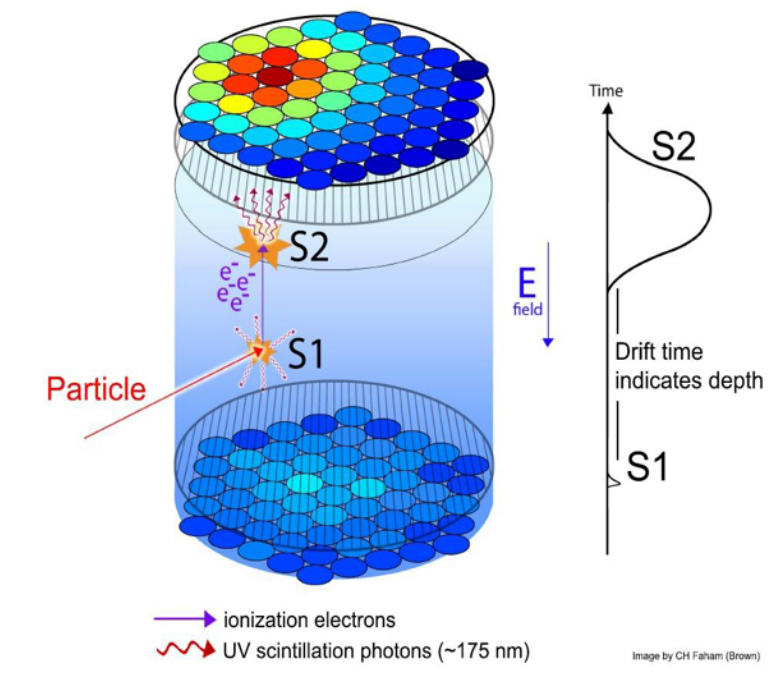
\includegraphics[width=150mm]{Figures/luxevent.png}
\caption{Schematic drawing of an event in the LUX detector. The initial event generates an initial burst of light, which is referred to a primary scintillation or $S1$, along with electron-ion pairs. The electrons are drifted to the liquid surface and extracted, causing a secondary burst of scintillation light, which is called the $S2$ signal. The x-y position of the event can be measured by the location of the $S2$ event, while the depth at which the event occurred is given by the time difference between the $S1$ and $S2$. This time delay is referred to as drift time. Figure taken from \cite{lux2012}.}
\label{fig:lux} 
\end{figure}

The free electrons are separated from the event site through the use of an an electric field, which is referred to as the drift field. They travel through this drift field until they reach the liquid/gas interface, where they were extracted with an efficiency of about 70\%. The electric field at the liquid/gas interface is set up so that is is about 5 kV/cm just below the surface and 10 kV/cm in the gas. These two field regions are referred to as the extraction field and electro-luminescence field. Once extracted from the liquid, an electron will be accelerated through the electro-luminescence field until it gains enough momentum to excite a gaseous xenon atom which in turn will emit a secondary scintillation photon. This process of acceleration, excitement, and scintillation, also known as ``proportional scintillation,'' continues to repeat until the electron reaches the anode. The collection of secondary scintillation light created by electron extraction is referred to as the $S2$. On average, a single extracted electron would create an $S2$ of about 25 photo-electrons.

The $S2$ light would be highly-localized in the plane of the liquid surface, which is also the plane of the PMT's and the wire-grids that create the drift and extraction fields. The plane was defined to be the x-y plane. The position of the event within the x-y plane was reconstructed by analyzing the relative signal size from the $S2$ in the top PMT array. The hottest PMT's in a given event would be those nearest the position from which the electrons were extracted. The x and y coordinates of an event could be reconstructed to within a few millimeters.

The depth, or z-position, of an event is given by the time separation between the $S1$ and $S2$. Electrons traveling through the detector will have a terminal drift velocity that depends on the drift field. In LUX the average drift velocity was about 1.5 mm per microsecond. Given a perfectly uniform electric field, the z-position of the event would be given the drift velocity times the drift time.


\subsection{Detector Construction}
Layouts of the internal structure of the LUX detector can be found in \ref{fig:lux_layout}, and a complete description of the construction and operational design of the LUX detector can be found in \cite{lux2012}. The inner xenon vessel is 39.75 inches tall and 24.25 inches in diameter and is contained within a larger outer vessel, which will contain the insulating vacuum. Both vessels are constructed of grade CP1 titanium in order to limit radioactive backgrounds, and are immersed in a water tank in order to provide shielding against thermal neutrons. An array of photo-multiplier tubes (PMT's) in the water tank allowed muon-coincident events to be vetoed from the data. There were also four source tubes that were submerged in the water tank. These tubes were installed against the outer-vessel and allowed for calibration of the detector using external sources.
\begin{figure}[!h]
\centering
\begin{subfigure}{0.5\linewidth}
\centering
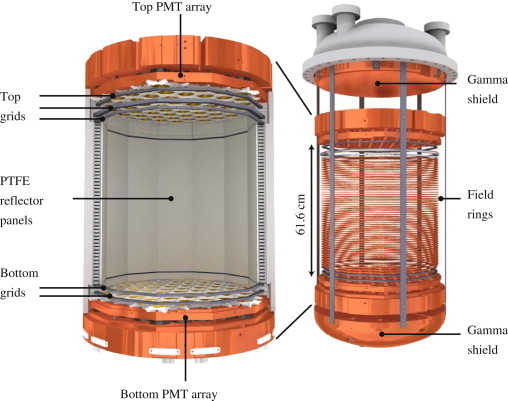
\includegraphics[width=\linewidth]{Figures/lux_internals.jpg}
\caption{}
\end{subfigure}%
\begin{subfigure}{0.5\linewidth}
\centering
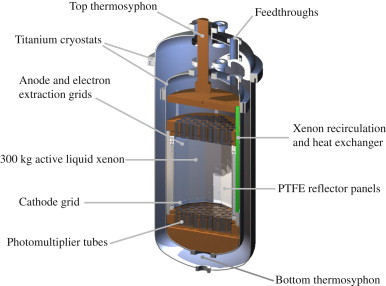
\includegraphics[width=\linewidth]{Figures/lux_layout.jpg}
\caption{}
\end{subfigure}
\caption{Layout of the LUX internals.\cite{lux2012}}
\label{fig:lux_layout} 
\end{figure}

The electric fields in LUX were set by five parallel-wire grids. There was a ``top'' and a ``bottom'' grid, which shielded the PMT arrays from seeing the full extent of the drift and extraction fields. The PMT's themselves are contained within two copper mounting blocks, with reflective Teflon covering the gaps between the PMT faces. The extraction field was set by the anode, which is about 1 cm above the liquid surface, and the gate grid, which is about 5 mm under the liquid surface. The drift field is set by the gate grid and the cathode, which are both submerged in the liquid, and are separated by by 49 cm. The uniformity of the drift field is enforced by a set of 48 field rings which are separated by 1 cm distance and are connected to their adjacent rings by two 1 G$\Omega$ resistors. The top ring is connected to the gate by a 0.875 G$\Omega$ resistor pair, and the bottom ring is connected to the cathode by a 1.25 G$\Omega$ resistor pair.

The field rings are supported by a UHMW polyethylene structure. The interior side of this structure is covered by 12 reflective Teflon panels. This gives the active xenon region a 47cm diameter, dodecagonal shape. Also embedded in the polyethylene structure is a 2-phase heat exchanger and a weir. The heat exchanger allows for heat transfer between the inlet and outlet sides of the xenon circulation, and the pour-over weir maintains a precise liquid level.

The temperature of the xenon is cooled and maintained at about 170K by a pair of copper shields at the top and bottom of the inner cryostat, which also act to block gammas. The copper shields themselves are cooled by a thermosyphon system\cite{thermosyphon}. A thermosyphon transfers heat from a cold head to a liquid nitrogen-cooled condenser through a double-walled tube filled with nitrogen gas. The nitrogen gas condenses on the condenser and drips down the inner wall until it reaches the cold-head. It vaporizes on the cold head and the newly warmed gas travels up the tube between the inner and outer walls back to the condenser. The cooling power can be regulated by adjusting the nitrogen pressure within the tube.

A gas recirculation system allowed the xenon to be constantly purified, which was done using a SAES
MonoTorr heated-zirconium getter\cite{getter}. The xenon was circulated through this getter by a diaphragm pump at a rate of about 20-25 standard liters per minute (SLM). Of this flow, 15-20 SLM came from the output of the 2-phase heat exchanger, and another 5 SLM came from instrumentation purge lines. This recirculation system also provided access to an in-situ sampling system for purity analysis, a liquid nitrogen cooled recovery vessel, the long-term xenon storage cylinders, and the tritium\cite{lux_tritium} and krypton-83m\cite{lux_kr1} internal-source injection systems. These injection systems are designing to mix samples of radioactive gasses into the xenon, allowing calibrations to be performed where the events are uniformly distributed throughout the active region.

\subsection{Data Structure}
There are three levels of data storage files used by LUX. All of the PMT waveform data that passes some minimum threshold is digitized into .dat files. This minimum threshold is defined such that any signal equal or greater than a single photo-electron will be digitized. 

These .dat files are fed into a set of code referred to as the ``Event Builder'', which filters the PMT waveforms into collections called ``events''. For an event to be triggered, a more stringent threshold must be crossed. This threshold requires, in part, multiple PMT's to fire in coincidence. When an event is triggered, an ``event window'' is defined, which spans 1 millisecond  before and after the event trigger. Peaks in the PMT waveforms found within this event window are further sorted into a set of 10 ``pulses''. The events and pulses are then stored in .evt files.

The highest level file is the .rq file. These files are output by the data processing framework, which sorts the pulses into $S1$, $S2$, single extracted electron, single photo-electron, or other. The framework also calculates all of the quantities of interest, such as the x-y positions, efficiency corrections, drift time, pulse timing, etc..


\subsection{Electric Field Model}\label{sec:efield}
After the preliminary WIMP-search run (Run03), and before the primary WIMP-search run (Run04), LUX underwent a grid conditioning campaign modeled after a burn-in period of a proportional counter. After this campaign was completed, it was found that the drift field had become highly non-uniform. The altered field is best explained by charge build-up on the Telfon panels.
\begin{figure}[!h]
\centering
\begin{subfigure}{0.5\linewidth}
\centering
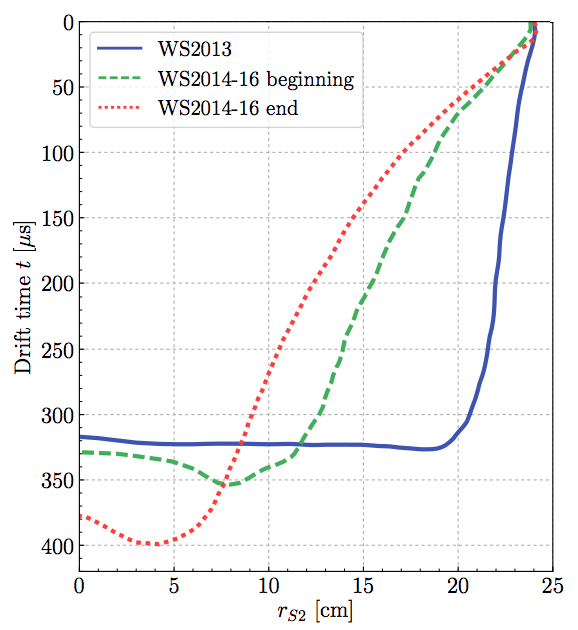
\includegraphics[width=\linewidth]{Figures/wall_radius.png}
\caption{}
\end{subfigure}%
\begin{subfigure}{0.5\linewidth}
\centering
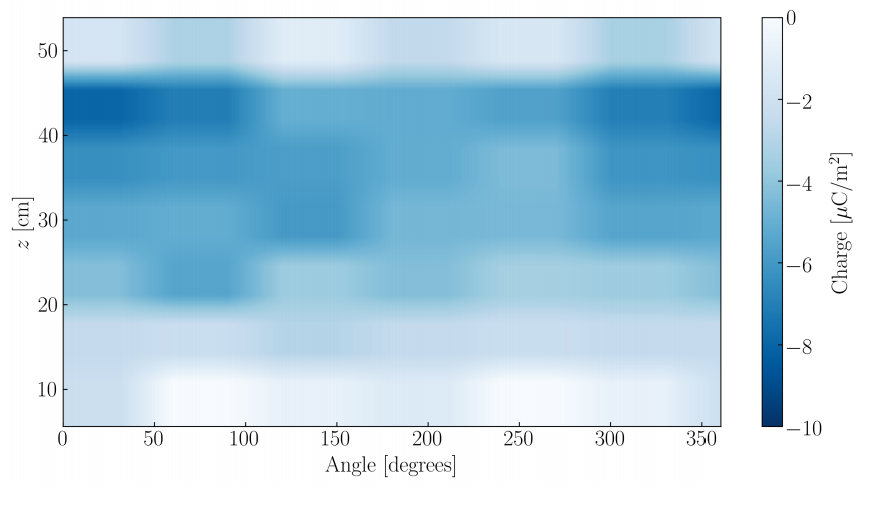
\includegraphics[width=\linewidth]{Figures/wall_charge.png}
\caption{}
\end{subfigure}
\caption{Here is shown the observed $S2$ x-y position of events at the wall of the detector (a), and an example of a best-fit charge distribution (b). The lines labeled WS2014-16 indicate data from the Run04 WIMP-search, and the WS2013 line shows the Run03 data. The reduction in wall radius at high drift times in the Run04 lines indicates that the drift field is highly non-uniform. The distribution of the wall-charge shown in (b) is for $^{83m}$Kr dataset from Kr data from 2014-10-06 and corresponds to the ``WS2014-16 beginning'' line. Figure taken from \cite{lux_efield}.}
\label{fig:lux_layout} 
\end{figure}

The uniformity of the drift field can be tested for by analyzing the distribution of $^{83m}$Kr events after an injection. The $^{83m}$Kr quickly becomes uniformly mixed throughout the active region, so the observed positions of the events should be uniformly distributed in drift time, as well as the x-y position of the $S2$. After the grid conditioning, it was found that at longer drift times the x and y position of the $S2$ became compressed. The distortion of the distribution indicated that a $^{83m}$Kr event that occurred near the wall of the detector (about 23.5 cm radius) at 300 microseconds drift time would have an $S2$ position of about 13 cm radius. Since electrons trace the electric field, this indicates that the field lines were not vertical and parallel, and that therefore the electric field was not uniform.

A comprehensive study of the drift-field in LUX was performed and is detailed in \cite{lux_efield}. For this analysis, the wall was divided into 42 tiles. A test-charge was placed on each of these tiles, and the resulting electric field was calculated using a COMSOL model. These 42 electric fields, along with a 0-charge field, are combined using the superposition principle, creating a net field that is used to generate a simulated $^{83m}$Kr dataset. The best-fit charge distribution is found by adjusting the weights of this superposition and comparing the resulting $^{83m}$Kr simulation to data.
 
 \subsection{Efficiency Corrections}\label{sec:krypcal}
The efficiency at which photons and electrons were converted into $S1$ and $S2$ varied depending on position at which they were generated. For instance, consider an event with energy $E$, number of photons, $N_{\gamma}$, and number of electrons, $N_e$. The top PMT array has a lower collection efficiency than the bottom array, so if this event took place near the top of the detector it would create a smaller $S1$ signal than if it were at the bottom. The $S2$ efficiency works in the opposite direction. Electrons generated near the bottom of the detector have to travel farther before they reach the liquid surface and therefore have a greater chance of being absorbed by a chemically active impurity. 

The average conversion factors from $N_{\gamma}$ and $N_e$ to $$S1$$ and $S2$ are referred to as $g1$ and $g2$:
\begin{equation}\label{eq:krypcal1}
\begin{split}
\langle S1 \rangle = N_{\gamma}g1\\
\langle S2 \rangle = N_e g2
\end{split}
\end{equation}
The variation in the efficiencies can therefore be thought of as a position dependence in these conversion factors ($g1=g1(xyz)$ and $g2=g2(xyz)$). We only have access to the ultimate $S1$ and $S2$ signals generated by an event, but the quantities we are interested in measuring are $N{_\gamma}$ and $N_e$. In order to extract these values, signal corrections are applied to $S1$ and $S2$ in order to remove the position dependence of $g1$ and $g2$. These corrections are defined:
\begin{equation}\label{eq:krypcal2}
\begin{split}
C_{S1}(xyz) \equiv \frac{g1(center)}{g1(xyz)}\\[1em]
C_{S2}(xyz)\equiv \frac{g2(top)}{g2(xyz)},
\end{split}
\end{equation}
where the center and top of the detector are indicated by $center$ and $top$. Then a single average value of each conversion factor is measured ($G1$ and $G2$) and used to calculate expected $N_{\gamma}$ and $N_e$ for an event with observed $S1$ and $S2$:
\begin{equation}
\begin{split}
\langle N_{\gamma} \rangle = \frac{S1_c}{G1}\\[1em]
\langle N_e \rangle = \frac{S2_c}{G2},
\end{split}
\end{equation}
where the subscript, $c$, represents an efficiency corrected value ($S1(2)_c=S1(2)\cdot C_{S1(2)}$).

While $g1$ and $g2$ vary with position, $N_{\gamma}$ and $N_e$ will depend on both the energy of the event, as well as the electric field. The non-uniform electric field described in the previous section means that an event with energy $E$, will produce a different $N_{\gamma}$ and $N_{e}$ depending on where it occurred in the detector. This is problematic to the measurements of $C_{S1}(xyz)$ and $C_{S2}(xyz)$. Typically the signal corrections are measured by assuming that $N_{\gamma}$ and $N_{e}$ from a line source will be constant throughout the detector. In this case, the efficiency corrections can be simply measured using:
\begin{equation}\label{eq:krypcal3}
\begin{split}
\frac{\overline{S1}(center)}{\overline{S1}(xyz)}\approx \frac{N_{\gamma}(center)g1(center)}{N_{\gamma}(xyz)g1(xyz)}\\[1em]
\frac{\overline{S2}(top)}{\overline{S2}(xyz)}\approx \frac{N_{e}(top)g1(top)}{N_{e}(xyz)g1(xyz)},
\end{split}
\end{equation}
where $\overline{S1}(xyz)$ and $\overline{S2}(xyz)$ are the average values measured from events at a given position, and we have made the approximation that $\overline{S1}(xyz)=\langle S1(xyz) \rangle$ and $\overline{S2}(xyz)=\langle S2(xyz) \rangle$. When $N_{\gamma}$ and $N_e$ are constant in position, as would be true for a line source in a uniform electric field, the terms $\frac{N_{\gamma}(top)}{N_{\gamma}(xyz)}$ and $\frac{N_{e}(top)}{N_{e}(xyz)}$ would cancel, leaving us with the expressions for $C_{S1}(xyz)$ and $C_{S2}(xyz)$ shown in equation \ref{eq:krypcal2}. 

Since the field was not uniform in LUX Run04 and onward, a field-correction had to be applied to the $S1$ and $S2$ signals before the efficiency-corrections could be found:
\begin{equation}\label{eq:krypcal4}
\begin{split}
S1_F\equiv S1 \frac{\langle N_{\gamma}(center) \rangle}{\langle N_{\gamma}(xyz)\rangle}\\[1em]
S2_F\equiv S2 \frac{\langle N_{e}(center)\rangle}{\langle N_{e}(xyz)\rangle}
\end{split}
\end{equation}
Here $S1_F$ and $S2_F$ are the field-corrected signals. Equation \ref{eq:krypcal2} can then be written
\begin{equation}\label{eq:krypcal5}
\begin{split}
C_{S1}(xyz) \equiv \frac{g1(center)}{g1(xyz)}=\frac{\langle S1(center) \rangle / N_{\gamma}(center)}{\langle S1(xyz) \rangle / N_{\gamma}(xyz)}\cdot \frac{N_{\gamma}(center)}{N_{\gamma}(center)} &\approx \frac{\overline{S1_F}(center)}{\overline{S1_F}(xyz)}\\[1em]
C_{S2}(xyz) \equiv \frac{g2(center)}{g2(xyz)}=\frac{\langle S2(top) \rangle / N_{e}(top)}{\langle S2(xyz) \rangle / N_{e}(xyz)} \cdot \frac{N_{e}(top)}{N_{e}(top)} &\approx \frac{\overline{S2_F}(top)}{\overline{S2_F}(xyz)}
\end{split}
\end{equation}

In Run04, the position-dependent efficiency corrections for the LUX $S1$ and $S2$ signals were obtained from a combination of tritium and $^{83m}$Kr calibration data using a procedure referred to as KrypCal\cite{richard}. The KrypCal procedure began with measuring  $C_{S2}$ using tritium. The field-dependence of $N_{e}$ are at a minimum at low-energy, so the use of tritium limits the systematic effects introduced by the estimation of $\frac{\langle N_{e}(center)\rangle}{\langle N_{e}(xyz)\rangle}$. This estimation is made using the existing NEST model, which will be introduced in the next section, and by making the approximation that the continuous tritium beta spectrum is actually a line source at 2.5 keV. To track $\overline{S2_F}$ as a function of position, the detector was binned in x, y, and z, and the tritium $S2_F$ spectrum in each bin was fit to a Landau function. The peak values of these Landau fits were taken to be $\overline{S2_F}$.

Tritium was only injected every 3 months or so, while the $^{83m}$Kr injections took place multiple times a week. For this reason, the ultimate measurements of $C_{S1}$ and $C_{S2}$ were made using krypton data. The field corrections for the krypton-83m events were derived using the preliminary tritium $S2$ corrections. Applying this preliminary efficiency correction to the $^{83m}$Kr $S2$ signals reveals the field dependence of $\langle N_{e}(xyz)\rangle$. Using the combined energy-model presented in section \ref{sec:combE}, the field dependence of $\langle N_{\gamma}(xyz)\rangle$ is derived from that of $\langle N_{e}(xyz)\rangle$. These field dependences give the field corrections for both the $^{83m}$Kr $S1$ and $S2$ signals. These field-corrections are propagated to each $^{83m}$Kr dataset, and the efficiency-corrections are calculated.

\section{Signals in Liquid Xenon and their Variations}
\subsection{The Combined Energy Model}\label{sec:combE}
When an energetic particle interacts with a target xenon atom it will create two measurable excitations, ions and excitons, with the rest of the energy being lost to heat. The expression for the energy of the interaction can then be written:
\begin{equation}\label{eq:combe1}
\begin{split}
E&=fW(N_*+N_i)\\
&=fW(1+\alpha)N_i,
\end{split}
\end{equation}
where $f$ is a loss factor to account for the energy that goes into heat, $N_*$ is the number of excitons generated in the event, and $N_i$ is the number of ions. The work function $W$ represents the average amount of energy it takes to produce a single ion or exciton. The quenching factor $f$ is constant for ER events, and so gets folded into the measurement of $W$. For NR events $f$ depends on the energy of the decay and so cannot be hidden in the same way. In these cases, the typical approach is to take $W=W_{ER}$ and to express $f$ in terms of the Lindhard factor, $L$\cite{lindhard}:
\begin{equation}
\begin{split}
E_{ER}=W(N_*+N_i)\\[1em]
E_{NR}=\frac{W}{L}(N_*+N_i)
\end{split}
\end{equation}
For ER events, the work function has been measured to be $W=13.7 \ \pm0.2$ eV/quanta\cite{dahl}. We have also defined the exciton-ion ratio $\alpha \equiv N_{*}/N_{i}$, which has been measured to be about 0.2\cite{doke2002,attila} for ER events and is typically assumed to be constant. In this document we will take $\alpha$ to have a constant value of 0.18 for ER events. 

Excitons are short-lived xenon molecules, Xe$_2^*$, in which a single excited xenon atom is able to bond with a ground state atom, in either a singlet or triplet state. The singlet state has a lifetime of about 3.1 ns, whereas the triplet state lives for about 24 ns\cite{pulseshape}. Both the singlet and triplet states decay to 2Xe by emitting two 178nm photons which contribute to the primary scintillation light ($S1$). Since these photons are emitted by the diatomic Xe$_2^*$, they are not readily absorbed by monatomic xenon and so will travel through the detector unimpeded. 

Some of the exciton-ion pairs will recombine to form additional Xe$_2^*$ molecules, and therefore also more primary scintillation light. The recombination process happens with a time constant of less than 50 ns\cite{rectime}. Assuming a fraction $r$ of electron-ion pairs recombine, the total number of photons $N_{\gamma}$ and electrons $N_{e}$ produced in an event would be given by:
\begin{equation}\label{eq:combe2}
\begin{split}
N_{\gamma}&=N_*+rN_i\\
&=(\alpha+r)N_i\\
N_e&=(1-r)N_i
\end{split}
\end{equation}
The recombination fraction, $r$, will be randomly distributed where both the mean value, $P_R$, and standard deviation, $\sigma_R$, depend on the decay energy and electric field.

Averaging equation \ref{eq:krypcal1} and combining with equations \ref{eq:combe1} and \ref{eq:combe2} yields a relation between the energy of an ER event and the average values of the observables, $S1_c$ and $S2_c$ :
\begin{equation}\label{eq:combe3}
E_{ER}=W(\frac{\overline{S1_c}}{G1}+\frac{\overline{S2_c}}{G2})
\end{equation}
Dropping the averages on the right side gives the expression for reconstructed energy: 
\begin{equation}\label{eq:combe3}
E_{rec}=W(\frac{S1_c}{G1}+\frac{S2_c}{G2})
\end{equation}
Reconstructed energy is an observable quantity that fluctuates around the true energy of the event, so can therefore be thought of as a measure of the true energy.
\begin{figure}[!h]
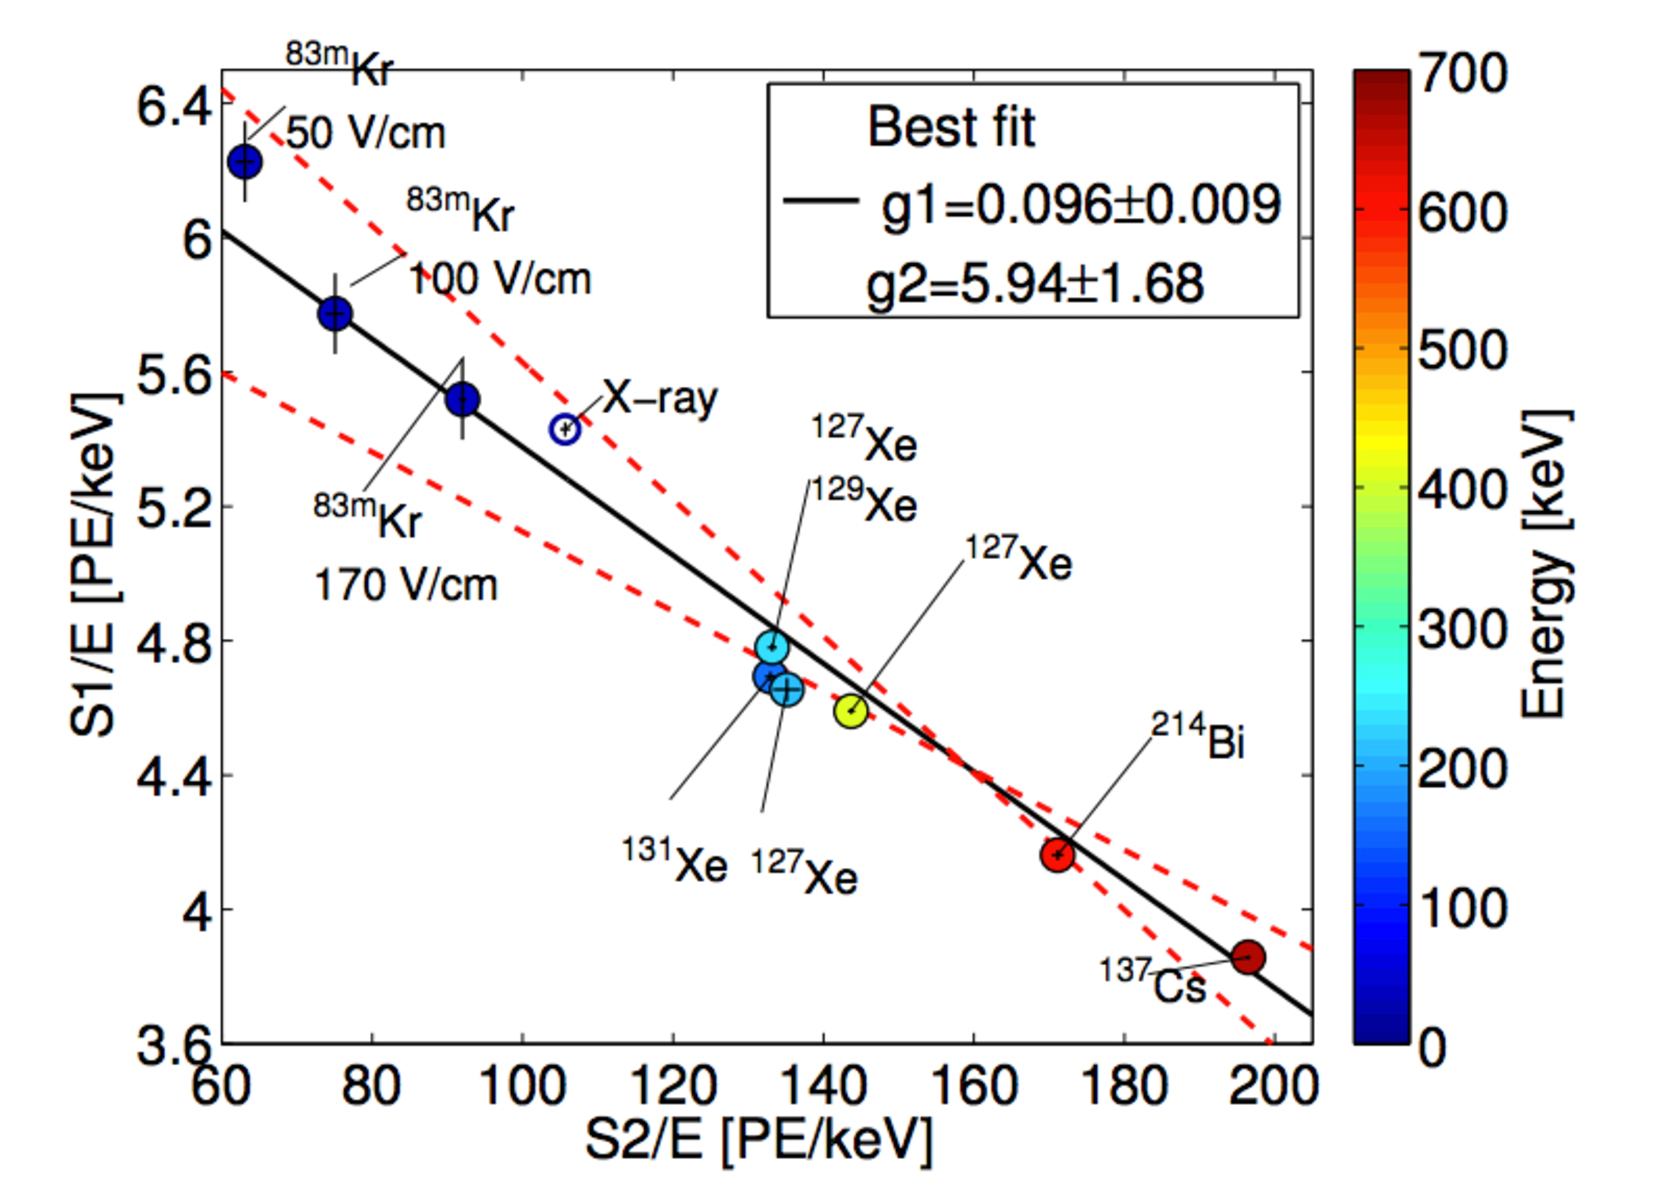
\includegraphics[width=\linewidth]{Figures/Doke_plot_run03.pdf}
\caption{Doke plot measured using various calibration lines in LUX Run03. Figure taken from \cite{attila}.}
\label{fig:lux_doke_plot} 
\end{figure}

Equation \ref{eq:combe3} also provides a useful tool in measuring the efficiency factors, $G1$ and $G2$. For an ER event with known energy $E$, we can write:
\begin{equation}
\left(\frac{W\overline{S1_c}}{E}\right)=-\frac{G1}{G2}\left(\frac{W\overline{S2_c}}{E}\right)+G1
\end{equation}
This equation has the form of a line where $y=\left(\frac{W\overline{S1_c}}{E}\right)$ and $x=\left(\frac{W\overline{S2_c}}{E}\right)$ are both in terms either measurable quantities or known constants. The efficiency factors, $G1$ and $G2$, can then be obtained by fitting a line through a set of (x,y) values measured at different energies and/or fields. This is referred to as the Doke plot method, and is the most common method for measuring $G1$ and $G2$\cite{doke2002}.

\begin{figure}[!h]
\centering
\begin{subfigure}{\linewidth}
\centering
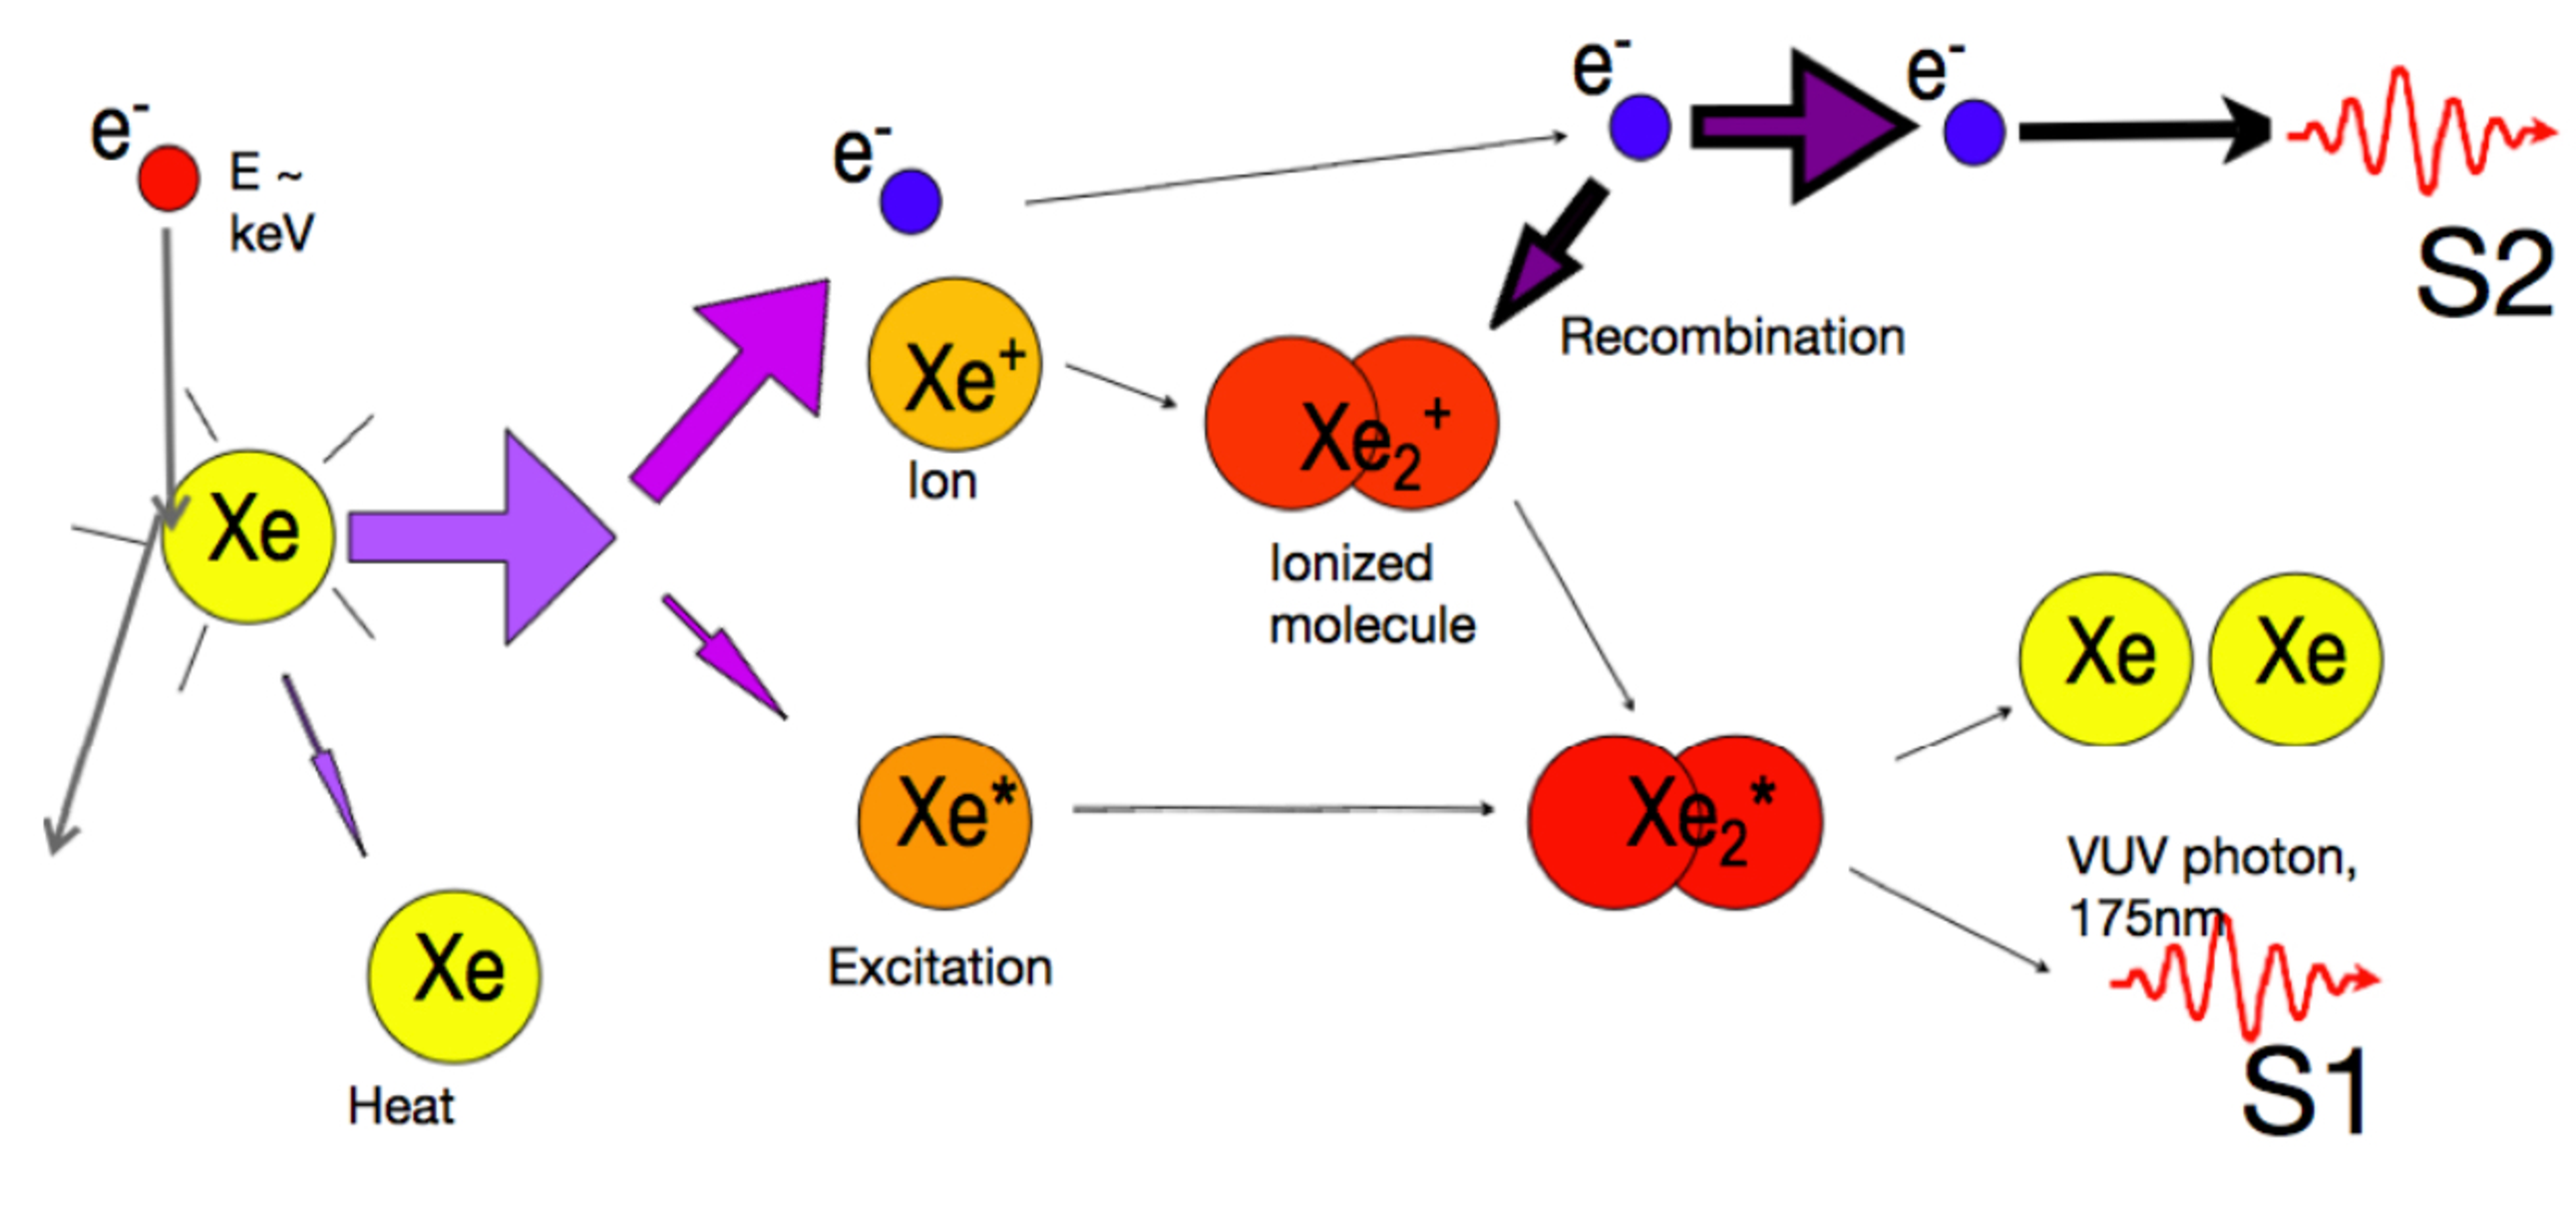
\includegraphics[width=\linewidth]{Figures/ER_diagram.pdf}
\caption{}
\end{subfigure}
\begin{subfigure}{\linewidth}
\centering
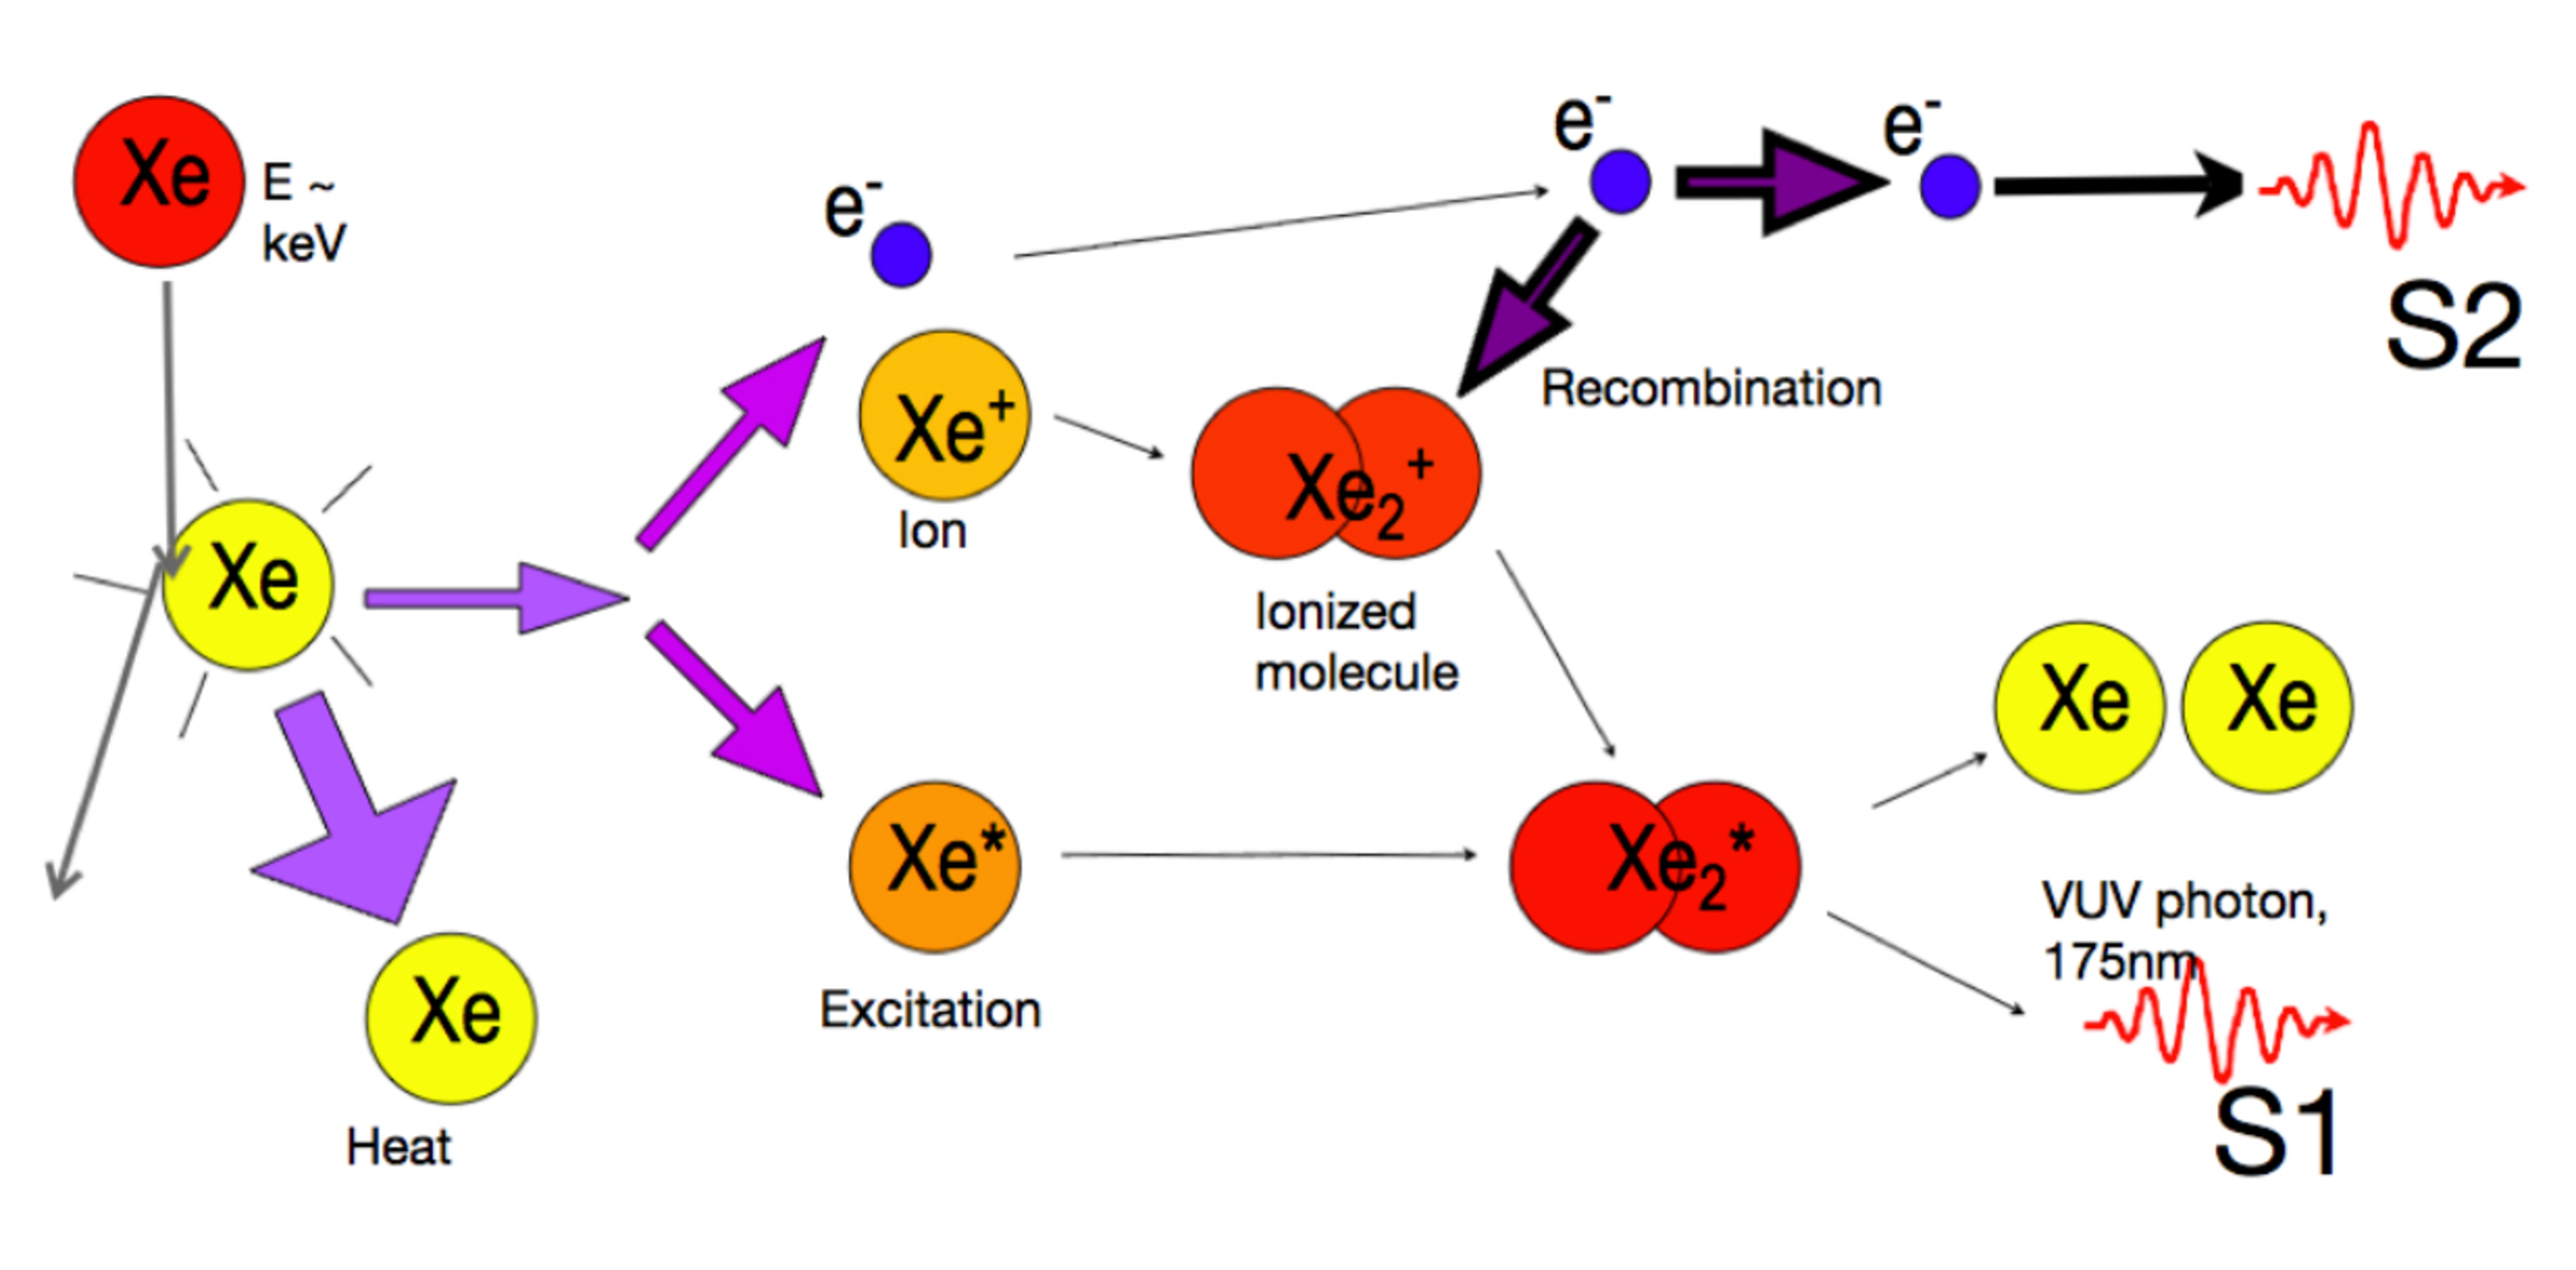
\includegraphics[width=\linewidth]{Figures/NR_diagram.pdf}
\caption{}
\end{subfigure}
\caption{Diagrams of an electronic recoil (a) and a nuclear recoil (b). These figures show how the deposited energy becomes partitioned between charge, light, and heat. In ER events, the amount of energy that goes into the heat channel is negligible. For NR events, however, a significant portion of the event energy is transferred to heat and is therefore not observed. Figures taken from \cite{attila}.}
\label{fig:lux_layout} 
\end{figure}



\clearpage

\subsection{Detector Resolution for Charge and Light Signals}\label{sec:detres}
On top of the fluctuations due to the recombination process, the $S1$ and $S2$ signals will also fluctuate due to detector variations. The $S1$ detector resolution, $\sigma_{\gamma,det}$ is composed of three parts: the binomial variance due to the finite light collection efficiency, $\epsilon_{\gamma}$:
\begin{equation}
\sigma_{S1,col}^2=N_{\gamma}G1(1-G1), 
\end{equation}
an additional variance due to a nonzero probability, $P_{DPE}$, that the PMT will experience double-photoemission\cite{DPE}:
\begin{equation}
\sigma_{S1,DPE}^2=G1\cdot N_{\gamma}P_{DPE}(1-P_{DPE}), 
\end{equation}
and the variance due to finite PMT resolution, $\sigma_{PMT}$:
\begin{equation}
\sigma_{S1,PMT}=N_{\gamma}G1\sigma_{PMT}^2
\end{equation}
The LUX signals were corrected for the double-photoemission effect, and so the $S1$ and $S2$ signals are measured in photons-detected (phd) rather than the typical photo-electrons (phe). For LUX post-Run04, we have $G1\approx 0.095$ phd per photon, $P_{DPE}\approx 0.2$, and $\sigma_{PMT}\approx 0.37$. Put together, this gives:
\begin{equation}
\begin{split}
\sigma_{S1,det}^2&=N_{\gamma}G1(1-G1+P_{DPE}(1-P_{DPE})+\sigma_{PMT}^2)\\
&\approx 0.11 \cdot N_{\gamma} \ \ (\text{phd}^2)
\end{split}
\end{equation}

The $S2$ signals are a bit more complicated because there are more steps between the initial generation of electrons, and the final detection of the secondary scintillation light. First, a fraction ($1-\kappa$) of the electrons will be lost as they travel from the interaction site to the liquid surface, and then another fraction will be lost due to finite extraction efficiency ($\epsilon_e$). We model these two effects with a single binomial distribution with probability equal to $\kappa\epsilon_e$. In LUX post-Run04, $\overline{\kappa} \approx 0.95$ and $\epsilon_e \approx 0.7$, so the total variance in the number of extracted electrons is:
\begin{equation}
\sigma_{ee}^2=N_e\cdot \kappa\epsilon_e(1-\kappa\epsilon_e)\approx 0.22 \cdot N_e \ (\text{phd}^2)
\end{equation}

Once the electrons are extracted, there will be added variance in the measured $S2$ from fluctuations in the number of photons generated by the electron cascade, as well as from photon detection fluctuations analogous to those for the $S1$ signal. These fluctuations can be folded together into the width of the single electron (SE) spectrum, which is easily measured. Measuring  SE spectrum is also useful because it allows the extraction efficiency to be separated from the total $G2$ value:
\begin{equation}
\epsilon_e=\frac{G2}{\mu_{SE}}
\end{equation}
In LUX post-Run04, $\mu_{SE}$ and $\sigma_{SE}$ were measured to be 24.5 and 5.3 phd, respectively. The total variance in $S2_c$ due to detector fluctuations will then be given by:
\begin{equation} 
\begin{split}
\sigma_{S2,det}^2&=N_e\cdot \kappa\epsilon_e(1-\kappa\epsilon_e)\mu_{SE}^2+N_e\cdot\kappa\epsilon_e\sigma_{SE}^2\\
&\approx 152 \cdot N_e \ (\text{phd}^2)
\end{split}
\end{equation}
 
The resolution of the reconstructed energy is given by:
\begin{equation}
\begin{split}
\sigma_{rec}^2&=W^2\left(\frac{\sigma_{S1,det}^2}{G1^2}+\frac{\sigma_{S2,det}^2}{G2^2}\right)\\[1em]
&=W^2\left((3.6)^2\cdot N_{\gamma}+(0.72)^2\cdot N_e \right)
\end{split}
\end{equation}
The energy resolution is therefore dominated by the $S1_c$ fluctuations. Assuming that $N_{\gamma}\approx N_e$, the energy resolution can be rewritten:
\begin{equation}
\sigma_{rec}^2\approx (0.3)^2\cdot E_{rec}
\end{equation}


\subsection{LibNEST: The Model Applied to LUX}\label{sec:libnest}
The Noble Element Simulation Technique (NEST) attempts to consolidate the various world measurements of energy deposition properties in liquid xenon into a single set of predictions\cite{nest1,nest2,lenardo}. The average charge and light signals measured experimentally are often reported using quantities referred to as light and charge yields:
\begin{equation}
\begin{split}
LY=\frac{\langle N_{\gamma}\rangle}{E}\\[1em]
QY=\frac{\langle N_e\rangle}{E}
\end{split}
\end{equation}
The number of photons and electrons for an event with energy $E$ can be calculated using the recombination model described in section \ref{sec:combE}:
\begin{equation}
\begin{split}
\langle N_{\gamma} \rangle=N_q\frac{\alpha +P_R}{1+\alpha}\\[1em]
\langle N_{e} \rangle=N_q\frac{1-P_R}{1+\alpha},
\end{split}
\end{equation}
where $P_R$ is the expected recombination fraction for the event, and is determined by the type of event, energy of the event, and applied drift field. The total number of quanta, $N_q$, is given by:
\begin{equation}
N_q=\frac{E}{W}=N_{i}+N_{*}=N_{\gamma}+N_{e}
\end{equation}
The equations for $LY$ and $QY$ can then be rewritten in terms of the recombination probability and the exciton-ion ratio, $\alpha$:
\begin{equation}
\begin{split}
LY=\frac{1}{W}\frac{\alpha +P_R}{1+\alpha}\\[1em]
QY=\frac{1}{W}\frac{1-P_R}{1+\alpha}
\end{split}
\end{equation}

The current version of NEST relies on a model or recombination probability known as the ``Thomas-Imel Box'' model for low energy events\cite{nest1,tib1,tib2}:
\begin{equation}\label{eq:tib}
P_R=1-\frac{\text{ln}(1+\xi)}{\xi} \text{, } \xi \equiv \frac{N_i \alpha'}{4a^2\nu}
\end{equation}
Here, $\alpha'$ characterizes the dielectric properties of liquid xenon, $a$ is a characteristic length scale of ion density, and $\nu$ is the mean ionization velocity of electrons. A more traditional model derived from Birk's Law is\cite{nest1}:
\begin{equation}\label{eq:birk}
P_R=\frac{A\frac{dE}{dx}}{1+B\frac{dE}{dx}}+C , \ B=A/(1-C)
\end{equation}
The quantity $\frac{dE}{dx}$ tends to increase with decreasing energy, so as $E$ goes to zero equation \ref{eq:birk} predicts that $P_R$ should approach unity. This would correspond $LY=1/W$ and $QY=0$. It has been observed, however, that for energies below about 20 keV, $LY$ begins to decrease, and $QY$ increases. This is the point at which the Thomas-Imel box model starts to become relevant. This corresponds to the point at which the track length of the energy deposit drops below the mean ionization distance in liquid xenon, about 4.6 microns. Equation \ref{eq:tib} does not depend on $\frac{dE}{dx}$ but rather $N_i$, and so it predicts the observed downward trend in $P_R$.  

Conceptually, this result is not too surprising and indicates that the probability that an electron will recombine with its parent ion is very small. This is referred to as geminate recombination, and its probability corresponds to $C$ in equation \ref{eq:birk}. If we consider a very low energy event in which only one ion is created, the only ion that the electron can recombine with is its parent so $P_R$ is identical to the geminate recombination probability. Therefore, the statement that $P_R$ goes to 0 at low energies also means that the geminate recombination probability is small.
\begin{figure}[!h]
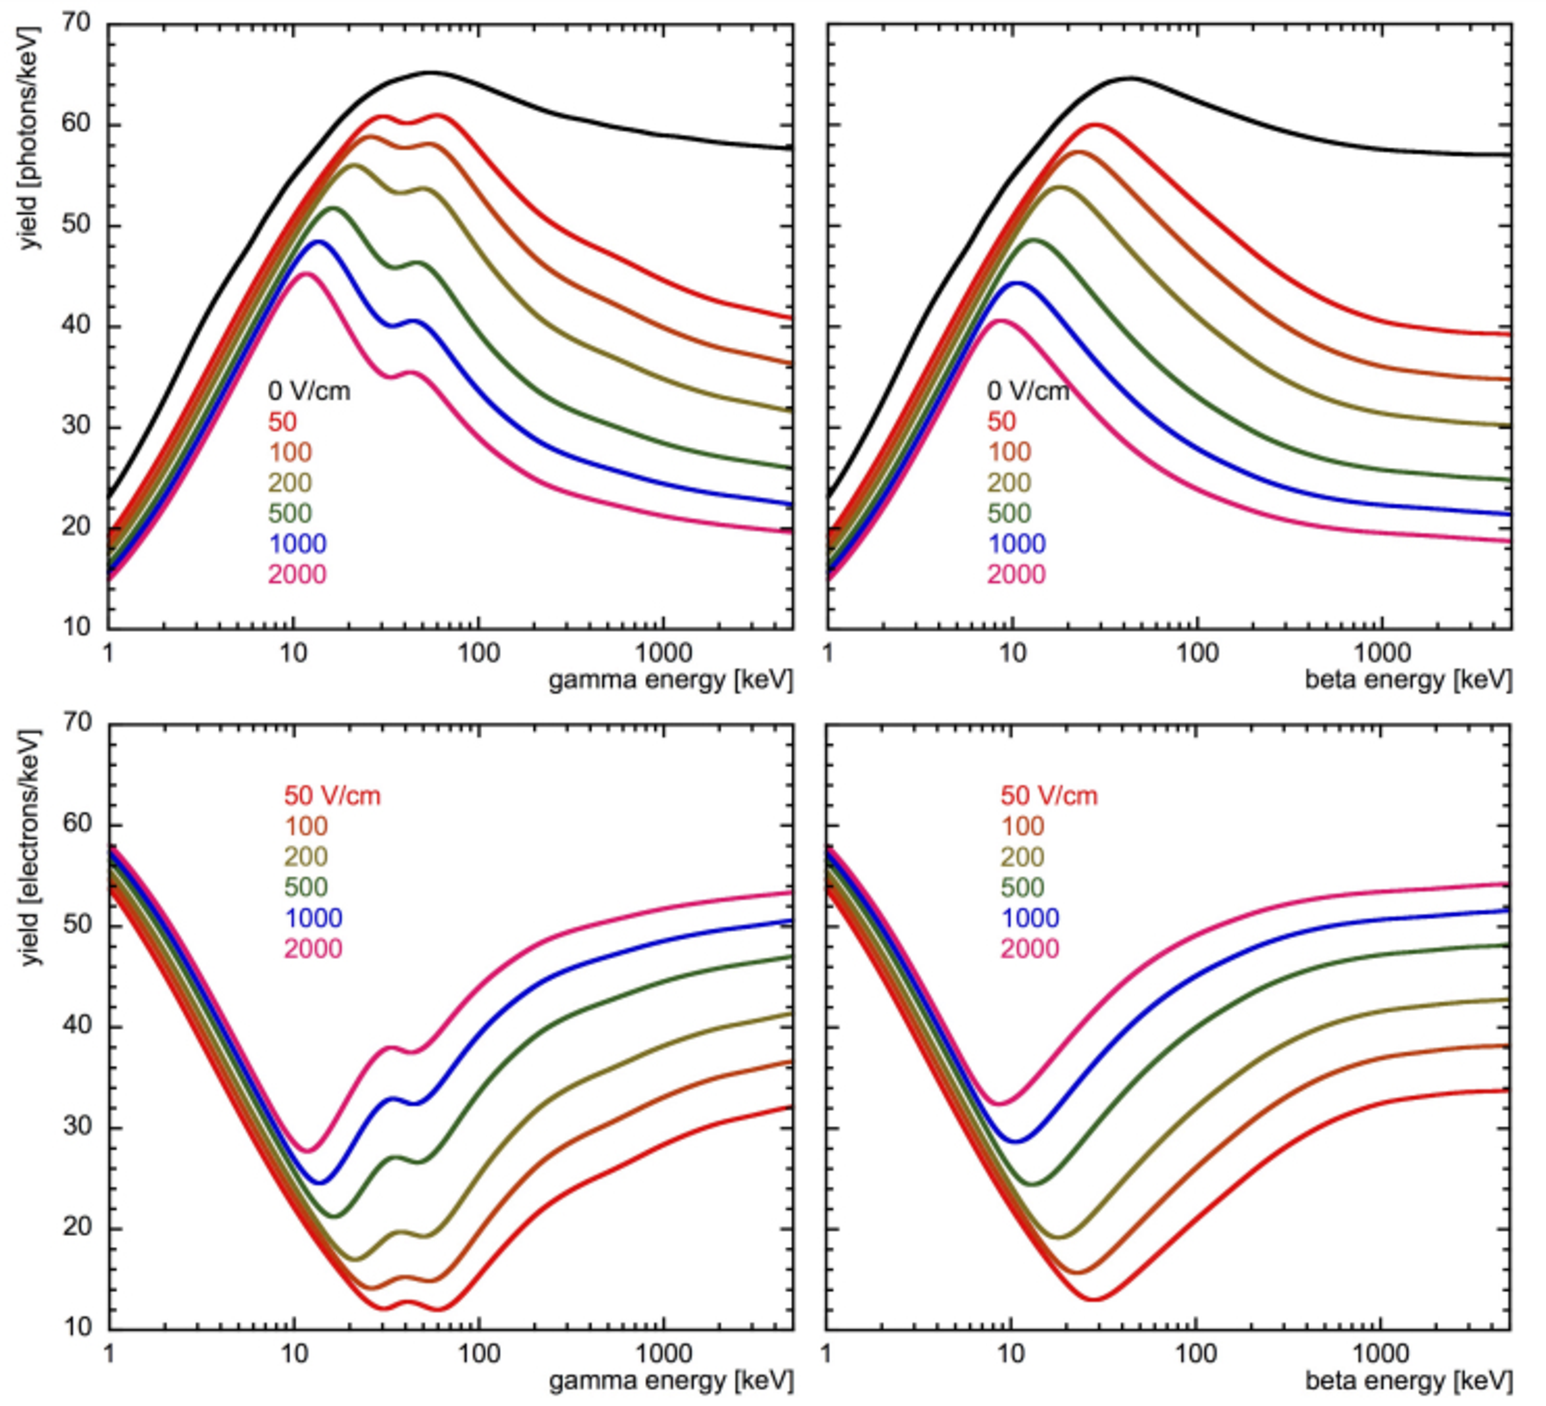
\includegraphics[width=\linewidth]{Figures/nest_yields0p98.pdf}
\caption{NEST v0.98 yield predictions for gamma (left) and beta/Compton (right) events. The bump in the gamma yields at 35 keV is due to photo-absorption at the K-edge x-ray site. Figure taken from \cite{nest2}.}
\label{fig:nest_yields0p98} 
\end{figure}

For ER energies less than 18.6 keV, NEST uses a Thomas-Imel model that is tuned to the LUX Run03 tritium data\cite{lux_tritium}. Above 122 keV, the model tuned to data such as xenon activation lines and $^{57}Co$. Measurements between these values have historically been sparse, so the light and charge yields are interpolated in this region. 


There are also considerations that must be made for whether the event is a beta of Compton scatter, or whether it is the photo-absorption of a gamma. The xenon K-edge x-ray will cause a resonance for gammas at 35 keV which is expected to increase the light yield in that region. The yield predictions from NEST v0.98 are shown in figure \ref{fig:nest_yields0p98}.

The recombination fluctuations are known to be greater than what would be expected for a binomial process. They have, in fact, been measured to grow approximately proportional to $N_i$\cite{attila}. NEST, therefore, models the recombination fluctuations using a Poissonian distribution, modified by a Fano-like factor, $F_RN_i$\cite{Evanyields}:
\begin{equation}
\sigma_R^2=(F_RN_i)\cdot (P_RN_i)
\end{equation}
\begin{table}[h!]
\centering
    \begin{tabular}{ c | c | c  }
    \hline
    parameter & description & value \\
    \hline \hline
    $G1^{\dagger}$ & average total light collection efficiency & 0.0931\\
    \hline
    $G2^{\dagger}$ & average total charge collection & 18.58\\
    \hline
    $\epsilon_e^{\dagger}$ & electron extraction efficiency ($G2$/$\mu_{SE}$) & 0.758\\
    \hline
    $\mu_{SE}$ & single electron mean & 24.5\\
    \hline
    $\sigma_{SE}$ & single electron width & 5.3\\
    \hline
    $\sigma_{PMT}$ & average resolution of PMTS & 0.37\\
    \hline
    $\kappa$ & probability of electron reaching liquid surface & sampled from $\frac{1}{C_{S2}}$\\
    \hline
    $F_R$ & Fano-factor for recombination fluctuations & 0.009975\\
    \hline
    \end{tabular}
    \caption{Values used in the libNEST model to simulate KrypCal corrected LUXdata in post-Run04 LUX data. The $\dagger$ superscript indicates values that will change when new efficiency corrections are introduced in section \ref{sec:corrections}.}
    \label{tab:libnestparms}
\end{table}


The libNEST code is a package developed for use with the LUX detector. It is designed to generate simulated LUX $S1$ and $S2$ signals given an input energy. It models the field and energy dependence of $N_{\gamma}$ and $N_e$ using the recombination model laid out in section \ref{sec:combE} and the NEST prediction of $P_R$ and $\sigma_R$. It then applies detector resolutions as described in section \ref{sec:detres} in order to generate the simulated $S1$ and $S2$ signals. The values of the parameters input into libNEST are shown in table \ref{tab:libnestparms}. This package will be used in chapters \ref{chap:4} and \ref{chap:5} of this document to model the effects of our new light and charge yield measurements on the $S1$ and $S2$ spectra for the ER calibrations conducted in LUX after the Run04 WIMP search.




\chapter{Building, Optimizing, and Maintaining a Xenon Cold-Trap Sampling System} \label{chap:sampling}





\section{Technical Overview}
A cold trap sampling system is designed to flow a sample of xenon with trace amounts of impurities through a section of liquid nitrogen cooled plumbing, to a mass-spectrometer for purity analysis. This document will deal particularly with krypton, but the method described also works for most simple impurities  such as helium, argon, nitrogen, oxygen, methane, etc.. Less volatile impurities such as water and large hydrocarbons tend to freeze along with the xenon, so are not detected. 

The operating principle is similar the that of freeze distillation. The bulk xenon is frozen to the cold plumbing leaving only the xenon ice vapor pressure at the output of the cold-trap. The flow of krypton is left largely unaffected. The resulting mixture which exits the cold-trap can be up up to $10^9$ times enriched in krypton. A cold-trap used in conjunction with a residual gas analyzer (RGA) whose sensitivity is about one part in $10^6$, is able to measure concentrations of krypton in a xenon sample down to the order of one part in $10^{15}$.
\begin{figure}[h]
  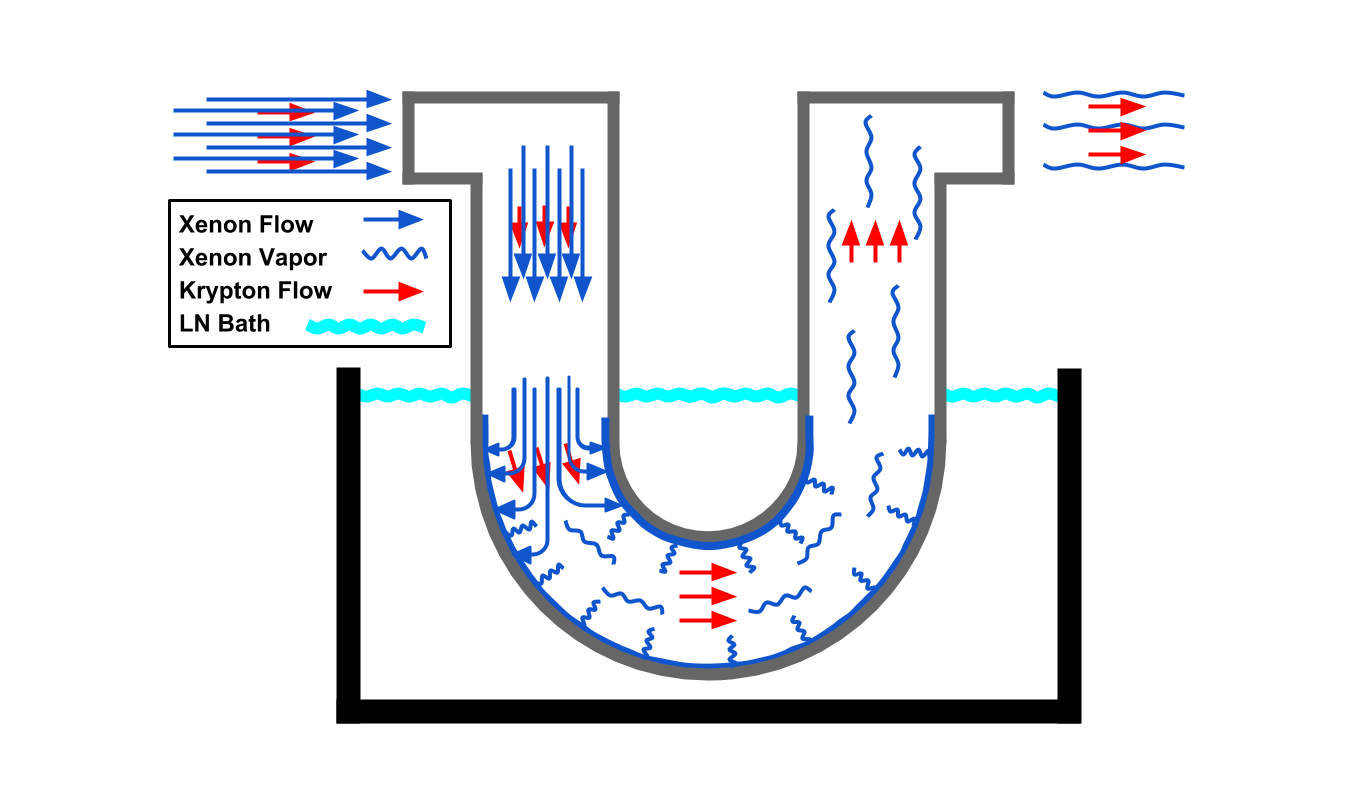
\includegraphics[width=\linewidth]{Figures/Cold_Trap_cartoon.png}
  \caption{Cartoon version of what happens during a cold trap analysis. }
  \label{fig:CTcartoon}
\end{figure}

\subsection{System Construction}
A cold trap sampling system should be laid out as described by figure \ref{fig:CTpid}. There will likely be additional transfer lines needed for collecting samples, recovering xenon, etc., but figure \ref{fig:CTpid} fully describes the plumbing necessary to analyze a sample of xenon.

\begin{figure}[h]
  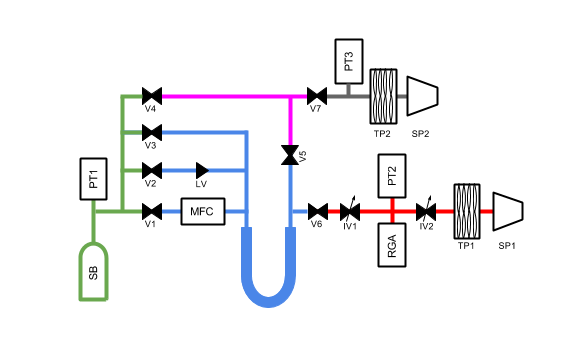
\includegraphics[width=\linewidth]{Figures/ColdTrap_diagram.png}
  \caption{Plumbing diagram of a general purpose cold-trap sampling system. The green section is referred to as the sample volume, the blue section is the cold trap volume, and the red section is the RGA volume. These are the sections used during analysis of a xenon sample. The pink section is the bypass line which serves two purposes. It is used to relieve pressure in the cold trap while the system is warming and acts as the access line to the pump-out turbo pump, TP2. }
  \label{fig:CTpid}
\end{figure}

The system should have 100\% metal-seals such as VCR or CF. Elastomer internals have the potential to become contaminated with krypton and destroy the sensitivity of the system and so should be limited.Traditionally, hardware used for this type of system is as follows:
\begin{itemize}
\item The plumbing should be entirely composed of UHP stainless steel.
\item The sample bottle, SB, is a \href{https://www.swagelok.com/en/product/Sample-Cylinders/DOT-Compliant}{1 gallon Swagelok DOT compliant sample cylinder}. 
\item The valves, V1 through V7 are some type of high purity shutoff valve. For automated systems, the \href{https://www.swagelok.com/en/product/Valves/Diaphragm-Sealed-Valves}{Swagelok DF series diaphragm valves} with pneumatic actuators are used. When possible, it is better to use the \href{https://www.swagelok.com/en/product/Valves/Bellows-Sealed}{Swagelok B series bellows valves} with the spherical copper stem tip option, since the DF series has a polymer seat, however these are more difficult to automate.
\item The sample pressure transducer is a capacitance manometer such as the \href{https://www.mksinst.com/product/category.aspx?CategoryID=72}{MKS Baratron} with a full scale of at least 3,000 Torr.
\item The leak valve, LV, is a metering valve.
\item The mass flow controller, MFC, should be metal sealed, and have a full range of about 10 SLM. The Celerity UNIT1660 is a good example. Although no longer in production, they are fairly easy to find used.
\item The cold trap itself is some UHP stainless steel plumbing that is bent or welded into a shape that allows it to be submerged in a liquid nitrogen bath. Currently, the optimal cold-trap geometry is a 1/2 inch ``stocking'' trap, as described in section \ref{sec:geometry}.
\item Traditionally IV1 has been a \href{https://www.swagelok.com/en/product/Valves/Bellows-Sealed}{Swagelok B series bellows valves} with the spherical copper stem tip option, however it's likely that the regulating stem tip would be better suited to the task. 
\item PT2 and PT3 are any cold cathode or inverted magnetron gauge that have an operating range of at least $10^{-8}$ to $10^{-4}$ Torr.
\item The residual gas analyzer, RGA, is the \href{http://www.thinksrs.com/products/RGA.htm}{SRS RGA200}.
\item IV2 needs to have a significantly lower impedance than IV1, so some type of 2.75" CF sealed all-metal vacuum valve should be used. A Varian UHV right angle valve, part No. 9515027 has been used in the past with good results.
\item TP1 and TP2 are turbo-molecular pumps with pumping speed of at least 70 liters per second. The Varian V70, V81, and V84 have all been used with good results.
\item SP1 and SP2 are the backing pumps for TP1 and TP2. They should be at least equivalent to the Agilent model SH110 scroll pump.
\end{itemize}  

\subsection{Operational Outline}
\label{sec:outline}
The exact steps required for a particular analysis can be quite complex, and some detailed example procedures can be found in  appendix \ref{ap:procedures}. A general outline of the operation of a cold trap sampling system is as follows:
\begin{enumerate}
\item A xenon sample is collected and stored in the sample volume until the beginning of analysis.
\item The system begins with all the valves closed.
\item  \label{step:analysis_start} The cold trap is immersed in a liquid nitrogen bath, and base layer of xenon ice is formed.
\item Baseline pressures are measured by the RGA by opening V6, exposing the RGA volume the the xenon ice vapor pressure present in the cold trap volume. Usually these baselines are established over a period of ten or more minutes.
\item \label{step:start_flow} Leaving V6 open, V1 or V2 is opened, allowing the xenon sample to freeze into the cold trap at a controlled flow rate. This will usually takes several minutes. 
\end{enumerate}
\noindent As described in figure \ref{fig:CTcartoon}, the xenon pressure at the RGA will remain constant during this step, but there will be a flow of krypton at the output of the cold-trap which will cause a rise in the krypton partial pressure in the RGA volume. It is this partial pressure pressure rise that will be analyzed to give the concentration of krypton in the xenon sample.
\begin{enumerate}[resume]
\item \label{step:stop_flow}After the sample volume has been exhausted, V1(2) will be closed, and the krypton partial pressure is allowed fall back to its prior value.
\end{enumerate}
\noindent At this point, the purity analysis of the xenon sample has been completed, but the system is not in a safe state. Only a microscopic amount of xenon has been pumped out through TP1, so the full mass of the xenon sample is frozen in the cold trap. If this is allowed to vaporize without proper precautions, the RGA and TP1 could be damaged by  over-pressure. It is therefore extremely important to isolate the RGA volume from the cold-trap volume before allowing the cold-trap to rise above liquid-nitrogen.
\begin{enumerate}[resume]
\item \label{step:analysis_stop} Close V6.
\end{enumerate}
\noindent If the sample mass was large enough, there could be enough xenon ice in the cold trap to damage the system instrumentation or even cause the plumbing system to rupture once it warms to the gas phase. This is why it is important to have rupture disks installed on the cold trap. To avoid damage to the system, the cold trap volume should be vented to the sample volume. Valve V3 provides a path from the input of the cold trap to the sample volume without the added impedance of the MFC or LV.
\begin{enumerate}[resume]
\item Open V3. 
\end{enumerate}
\noindent This is where the bypass line comes in. With a cold-trap made from 1/2" plumbing, it is likely that an ice blockage will form once the xenon flow has stopped. This ice blockage could cause a dangerous pressure differential between the input and output of the trap. By opening the bypass line, the output of the cold trap has a second path to the sample volume.
\begin{enumerate}[resume]
\item Open V4 and V5. 
\end{enumerate}

The system is now in a safe state and the cold trap can be allowed to warm back to room temperature. The remaining xenon can then be recovered or discarded as desired, after which the system should be pumped to vacuum before collecting the next sample. It is important to note that this pump-out should be done using TP2, since the RGA volume should be kept at vacuum except for maintenance. The bypass line, as configured, allows the cold-trap volume and sample volume to be pumped out independent of one another.

\section{Idealized Cold Trap Response}
\label{sec:vaceq}
In order to optimize the sensitivity of the cold-trap system, it is good to have an understanding of the basics of vacuum physics. A vacuum system can be analogized to an electrical circuit, with pressure taking the place of voltage, flow rate ($Q$) taking the place of current, and impedance ($Z$) taking the place if resistance. This analogy gives us with the equation:
\begin{equation}
\label{eq:vaclaw1}
\Delta P = Q\cdot Z
\end{equation} 
An important note here: in this document we use the generic $P$ to denote a pressure at any specific point in the system, but reserve $PP_{s}$ to represent the partial pressure of some species, $s$, as measured by the RGA. For instance, $PP_{Kr}$ will refer to partial pressure of $^{84}Kr$ as it is measured by the RGA, whereas $P_{Kr,CT}$ will used to represent the krypton pressure present in the cold trap. 

Returning to the vacuum equations, it is now useful to define a new quantity, $S$, which is called the ``volumetric flow rate" or ``pumping speed''. $S$ is defined: 
\begin{equation}
\label{eq:volflow}
S \equiv Av = \frac{dV}{dt}=Q/P, 
\end{equation}
where $A$ is the cross-sectional area of the pipe, and $v$ is the flow velocity, and $dV$ is the volume of gas which passes a point in the system in time $dt$. An effective pumping speed can be calculated for any point in the vacuum system through the equation:
\begin{equation}
\label{ep:vacimp}
1/S_{eff} = 1/S_{p}+Z_{total}, 
\end{equation}
where $S_{p}$ is the speed of the pump which is acting on the system, and $Z_{total}$ is the total impedance between the pump and the specified point in the system. We can then calculate the steady-state pressure at any point in the system\cite{vac_eq}:
\begin{equation}
\label{eq:vaclaw2}
P=Q/S_{eff}.
\end{equation}


\subsection{Vacuum Impedances}
The calculation of system impedances depends on which flow regime a gas resides. The flow regime is determined by whether a given gas molecule interacts primarily with other molecules, or with the walls of the vacuum chamber. The flow regime can be characterized by the Knudsen number, $K \equiv \lambda/d$, where $\lambda$ is the mean free path, and $d$ is the inner diameter of the vacuum chamber. For $K>>1$, a gas molecule is very likely to encounter the wall of the system before encountering another gas molecule; this is the molecular flow regime. When $K<<1$, the system is in the viscous flow regime where a gas molecule will be interacting predominantly with other gas molecules. If $K$ is $O(1)$, the system is in what is referred to as the intermediate regime.\cite{vac_eq}

In the molecular flow regime the impedance of a system element will depend on the geometry of the element, and on the molecular weight and temperature of the gas in question, but it will not depend on the pressure of that gas. For instance, the impedance of an aperture with area $A$ will be given by:\cite{vac_eq}
\begin{equation}
\label{eq:aperture}
Z=\sqrt{\frac{2\pi M}{8kTA^{2}}}.
\end{equation}

In the intermediate regime, the impedance picks up a complicated pressure dependance that can not be exactly calculated. Xenon gas inside the cold trap is at $1.8\times 10^{-3}$ Torr and 77 Kelvin.\cite{vaporpressure} In a $0.5"$ diameter cold trap the xenon has a Knudsen number of 0.6. This puts this section of plumbing in the intermediate gas flow regime rather than the molecular flow regime, and limits the accuracy of any results calculated using the molecular flow approximation. The role of vacuum equations in this document is to provide qualitative predicts on how the krypton pressure at the RGA will behave in response to changes in system parameters. The exact response of the system is always characterized empirically, as will be described in section \ref{sec:calibrations}. For this purpose, the molecular flow approximation will suffice to motivate and direct our empirical investigations.\cite{vac_eq}

The particular impedances of interest here are impedance between the cold-trap and the RGA ($Z_1$) and the impedance between the RGA and TP1 ($Z_2$). IV1 and IV2 are in place so that $Z_1$ and $Z_2$ can be fine tuned to an optimal arrangement. This optimization will be described further in section \ref{sec:impedance}, but first there is a hard constraint that must be placed on the relative values of $Z_1$ and $Z_2$.

The RGA has a maximum operating pressure of $1\times 10^{-6}$ Torr, although we have found that operating at about $1\times 10^{-5}$ Torr is possible with minimal degradation of the CDEM. When analyzing xenon samples with a concentration of about one part per million or less, the xenon partial pressure, $PP_{Xe}$,  will dominate the absolute pressure at the RGA. $PP_{Xe}$ is the sourced by the vapor of the xenon ice in the cold trap, which is $P_{ICE}=1.8\times 10^{-3}$ Torr, and so needs to be reduced by a factor of about 100 or more between the cold-trap and the RGA\cite{vaporpressure}. 

There are several compounding factors that come into play when deciding exactly what $PP_{Xe}$ should be. These will be discussed in later sections, so we will take it as given here that the sensitivity is optimized between $PP_{Xe}=5\times10^{-6}$ Torr, and $PP_{Xe}=2\times10^{-5}$ Torr, and is largely unaffected by deviations within this range. For the sake of simplicity, we will usually demand that $PP_{Xe}$ to be the default pressure that the system plumbing gives when IV1 and IV2 are maximized. For the system described above, the this pressure will be about $1\times 10^{-5}$ Torr. 

To avoid saturation and mass-dependent effects of the RGA, we often use the doubly-ionized peak of the xenon-124 isotope as our measure $PP_{Xe}$. This peak appears at 62 amu, and so will be referred to as $PP_{Xe62}$. When the system is properly adjusted, $PP_{Xe62}$ should be around 1,000 pTorr, or $1\times 10^{-9}$ Torr.

Returning to the vacuum equations we will see that although we have artificially defined $PP_{Xe}$, $Z_1$ and $Z_2$ are not fully determined by this choice. By using equations \ref{eq:vaclaw1} and \ref{eq:vaclaw2}, and the requirement that $PP_{Xe}=1\times 10^{-5}$ Torr, we place a constraint on the impedances:
\begin{equation}
\label{eq:xepres1}
Q_{Xe,RGA}=PP_{Xe}S_{RGA}=\frac{P_{ICE}-PP_{Xe}}{Z_1}\approx \frac{P_{ICE}}{Z_1},
\end{equation}
where $1/S_{RGA}=1/S_{TP1}+Z_2$. This gives,
\begin{equation}
\label{eq:impconstraint}
S_{RGA}\cdot Z_1= \frac{P_{ICE}}{PP_{Xe}} = 180.
\end{equation}
$S_{RGA}$ is usually dominated by $Z_2$. Depending on the model of pump used, the speed of the turbo pump for xenon is around 50 liters per second. The impedance of cylindrical plumbing with a diameter of 1.5 inches is about $\frac{1}{320} s/L$ per centimeter of plumbing.\cite{vac_eq} In a typical system there will be the equivalent of about 5 feet of plumbing between the RGA and TP1, so the nominal value of $Z_2$ will be roughly 0.48 seconds per liters for xenon, indicating a maximum $S_{RGA}$ of 2.1 liters per second.\cite{vac_eq} This means the fully-open value of $Z_1$ should be about 85 seconds per liter for xenon. The exact numerical value of $S_{RGA}$ and $Z_1$ are largely unimportant, and when optimizing the system impedances as described in section \ref{sec:impedance}, we will work in units relative to the fully open state, rather than liters per second.



\subsection{Setting System Impedance}
\label{sec:imp_set}
The sensitivity of a cold trap sampling system depends upon $Z_1$ and $S_{RGA}$. We can adjust IV1 and IV2 to change $Z_1$ and $S_{RGA}$, but wish to do so in a reproducible way. To this end, we look to the left hand side of equation \ref{eq:impconstraint} and see that $PP_{Xe}$ is proportional to $1/S_{RGA}Z_1$. If we adjust IV1 while holding IV2 constant, we can use $PP_{Xe}$ as a measurement of $Z_1$ relative to its fully open state. Once $Z_1$ has been adjusted to a desired set-point, we can use IV2 to adjust $S_{RGA}$ until $PP_{Xe}$ is restored to its pre-adjustment value.

For example, take the RGA trace shown in figure \ref{fig:imp_adj}. In this case, $PP_{Xe62}= 710 \pm30$ pTorr when IV1 and IV2 are both fully open (region \emph{I} in the figure). This state will be referred to as the 1x impedance state. In region \emph{II} of figure \ref{fig:imp_adj} IV1 is partially closed until $Z_1$ has increased by a factor of $19\pm2$. This has the effect of decreasing $PP_{Xe62}$ from $710\pm30$ pTorr in region \emph{I} to $38\pm5$ pTorr in region \emph{III}. In Region \emph{IV}, $S_{RGA}$ is incrementally reduced by adjusting IV2 until $PP_{Xe62}$ returns to $710\pm40$ pTorr. This final state (region \emph{V}) will be referred to as the 19x impedance state. 

Equation \ref{eq:aperture} shows that $Z_1$ will have a dependence on the molecular mass of the gas in question. The $\sqrt{M}$ dependence means that the impedance for $^{84}$Kr ($Z_{1,Kr}$) will be about 18\% lower the impedance for $^124$Xe. This is another reason to work in units of relative impedance rather than absolute impedance. A factor of 19 increase in impedance to xenon will mean that the impedance for krypton will also have increased by a factor of 19.

\begin{figure}[h!]
\centering
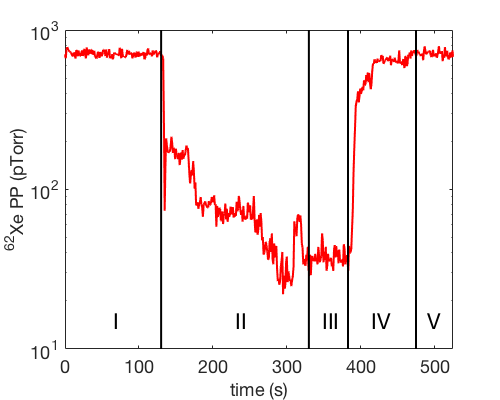
\includegraphics[width=\textwidth]{Figures/impedance_adjust.png}
\caption{Adjustment of impedance to 19x state. Region \emph{1} shows the fully-open, 1x impedance state of the system. In region \emph{II}, $Z_1$ is manually reduced using IV1, until region \emph{III}, where $PP_{Xe62}$ has dropped to 1/19$^{th}$ of its value in the 1x impedance state. In region \emph{IV}, $PP_{Xe62}$ is carefully increased back to its initial value by slowing down the effective pumping speed, $S_{RGA}$. In region \emph{V}, $PP_{Xe62}$ has returned to its initial value, and the system is in the 19x impedance state. }
\label{fig:imp_adj}
\end{figure}


\subsection{Generalized Cold Trap System Response}
\label{sec:response}
The operating principle of cold-trap sampling is that while the xenon gets frozen into the cold-trap, the trace gasses, such as krypton pass through. Another way to put this is that at the output of the cold trap the xenon is frozen to a constant pressure, while krypton mass flow is conserved. In practice, the conservation is not perfect, so we add a throughput constant, $\alpha \equiv Q_{Kr,RGA}/Q_{Kr,CT}$, where $Q_{Kr,CT}$ is the flow rate into the cold trap, and $Q_{Kr,RGA}$ is the equilibrium flow rate of krypton out of the trap, and the flow rate of xenon into the cold-trap ($Q_{Xe,CT}$) is constant. $Q_{Kr,CT}$ is equal to $Q_{Xe,CT}$ times the concentration of krypton in the xenon sample, $\Phi_{Kr}$. These relations put together, give us the following equation: 
\begin{equation}
Q_{Kr,RGA}=\alpha Q_{Xe,CT}\Phi_{Kr}.
\end{equation}
Plugging this into the vacuum equations, we can find the relationship between the parameter of interest, $\Phi_{Kr}$, and the measurable quantities, $Q_{Xe_0}$ and $PP_{Kr,eq}$:
\begin{equation}
\label{eq:krpres1}
PP_{Kr,eq}=\frac{\alpha}{S_{RGA}}Q_{Xe,CT}\Phi_{Kr}.
\end{equation}
This relation shows the proportionality between partial pressure, and flow-rate times concentration that was found experimentally in \cite{sampling_doug} and \cite{sampling_dm}. By imposing the constraint from equation \ref{eq:impconstraint} we can see how altering the system impedance is expected to affect $PP_{Kr,eq}$, the equilibrium pressure of krypton at the RGA:
\begin{equation}
\label{eq:krpres2}
PP_{Kr,eq}=\frac{\alpha}{180}Z_{1}Q_{Xe,CT}\Phi_{Kr}.
\end{equation}

From the vacuum equations, we can also find the expected response of the system to an impulse of krypton. To do so, we would like to make the assumption that the RGA volume and the cold trap volume have a vanishingly small internal impedance, which means that the pressure at the input is equal to the pressure at the output. This is reasonable for the RGA volume which is constructed of 1.5 inch plumbing. However, we find that the bends in the cold trap plumbing cause this approximation to break down in when the xenon ice extends past the first leg of the trap. The effects of this breakdown will be discussed in a later section, but for now we will remain in the limit of small xenon flow rate and small xenon sample size where the approximation does provide largely valid predictions.

In a volume with no internal impedance, the amount of krypton contained by that volume is defined as $P_{Kr}V$. If the volume is being evacuated at a constant volumetric rate, $S$, while at the same time being sourced by some time-dependent flow rate, $Q(t)$ the amount of krypton will change according to the equation:
\begin{equation}
\label{eq:expdiff}
V\frac{dP_{Kr}}{dt}=Q(t)-SP_{Kr}.
\end{equation}
The response of $P_{Kr}(t)$ to an impulse of flow, $Q(t)=P_0V\delta(t)$ is then:
\begin{equation}
P_{Kr}(t>0)=P_0e^{-t/\tau},
\end{equation}
where $\tau = V/S$. The time dependent $P_{Kr}(t)$ can then be found by convolving $Q(t)$ with this impulse response.

Applying this impulse response to the RGA volume ($V_{RGA}$) and cold trap volume ($V_{CT}$), we can find an expected time dependence of the krypton RGA pressure, $PP_{Kr}(t)$. The flow rate into the RGA volume is equal to the flow rate out of the cold trap volume, so it is given by:
\begin{equation}
Q_{Kr,RGA}(t)=\frac{P_{Kr,CT}(t)}{Z_1+1/S_{RGA}}\approx P_{Kr,CT}(t)/Z_1,
\end{equation}
where $P_{Kr,CT}(t)$ is the time-dependent pressure of krypton in the cold trap volume. So to calculate the expected $PP_{Kr}(t)$, we must first calculate $P_{Kr,CT}(t)$. This can be done by convolving the the known flow of krypton into the trap, $Q_{Kr,CT}=\Phi Q_{Xe,CT}(t)$, with the impulse response of the cold trap volume. We can then convolve the resulting $Q_{Kr,RGA}(t)$ with the response of the RGA volume to predict the overall response of the system to the input flow rate. 

The response time for the cold trap volume will be given by:
\begin{equation}
\tau_{CT}=V_{CT}\frac{1}{Z_1+1/S_{RGA}} \approx V_{CT}Z_1,
\label{eq:CTtime}
\end{equation}
and the response time for the RGA volume will be given by:
\begin{equation}
\tau_{RGA}=V_{RGA}/S_{RGA}.
\end{equation}
The condition $Z_1S_{RGA}=180$ from equation \ref{eq:impconstraint}, combined with the fact that in a typical system, $V_{RGA}\approx V_{CT}$, means that the RGA volume is expected to respond much more quickly than the cold trap volume. Therefore the overall response of the system will be dominated by the response of the cold trap, and the shape of $PP_{Kr}$ will be well approximated by the shape of $P_{Kr,CT}$.

In this document we use flow rate profiles for xenon of the form:
\begin{equation}
\label{eq:flowprofile}
Q_{Xe,CT}(t) =
  \begin{cases}
    Q_0&\textrm{ for } \leq t\leq T\\
    0     &\textrm{ otherwise}
  \end{cases}
\end{equation}
If $Q_{Xe,CT}(t)$ is given by equation \ref{eq:flowprofile}, the instantaneous krypton pressure in the cold trap will be given by: 
\begin{equation}
\label{eq:CTresponse1}
\frac{P_{Kr,CT}(t)}{\Phi Q_0Z_1}=
\begin{cases}
0 & \textrm{ for } t<0\\
1-e^{-\frac{t}{\tau_{CT}}} & \textrm{ for } 0\leq t \leq T\\
(1-e^{-\frac{T}{\tau_{CT}}})e^{-\frac{t-T}{\tau_{CT}}}& \textrm{ for }  t > T
\end{cases}
\end{equation} 
Applying the response of the RGA volume gives the result:
\begin{equation}
\label{eq:fullresponse}
\frac{PP_{Kr}(t)}{\Phi Q_0 /S_{RGA}}=
\begin{cases}
0 & \textrm{ for } t<0\\
1-e^{-\frac{t}{\tau_{RGA}}}-\frac{e^{-\frac{t}{\tau_{CT}}}-e^{-\frac{t}{\tau_{RGA}}}}{1-\tau_{RGA}/\tau_{CT}} & \textrm{ for } 0\leq t \leq T\\
e^{-\frac{t-T}{\tau_{RGA}}}(1-e^{-\frac{T}{\tau_{RGA}}}-\frac{e^{-\frac{T}{\tau_{CT}}}-e^{-\frac{T}{\tau_{RGA}}}}{1-\tau_{RGA}/\tau_{CT}} ) ...\\
 +\frac{e^{\frac{T}{\tau_{CT}}}-1}{1-\tau_{RGA}/\tau_{CT}}(e^{-\frac{t}{\tau_{CT}}}-e^{-\frac{t}{\tau_{RGA}}+T(1/\tau_{RGA}-1/\tau_{CT})}) & \textrm{ for }  t > T
\end{cases}
\end{equation} 
When $\tau_{RGA}<<\tau_{CT}$, the right side of equation \ref{eq:fullresponse} reduces to the right side of equation \ref{eq:CTresponse1}. Combining this with the constraint from equation \ref{eq:impconstraint} yields:
\begin{equation}
\label{eq:CTresponse}
PP_{Kr}(t)=\frac{Z_1 Q_0}{180}\Phi
\begin{cases}
0 & \textrm{ for } t<0\\
1-e^{-\frac{t}{\tau_{CT}}} & \textrm{ for } 0\leq t \leq T\\
(1-e^{-\frac{T}{\tau_{CT}}})e^{-\frac{t-T}{\tau_{CT}}}& \textrm{ for }  t > T
\end{cases}
\end{equation} 

Equation \ref{eq:CTresponse} does a good job in predicting the shape of $PP_{Kr}$ when $Q_0$ and $Z_1$ are small as seen in figure \ref{fig:RGAtrace_fast}. A fit to equation \ref{eq:CTresponse} produces a best fit time constant of 12.2 seconds. We measure the volumes spaces in our system by volume sharing with a known volume. The volume of the cold trap used in this trace was 183.8 cc, which would point to $Z_1=66.7$ seconds per liter and $S_{RGA}=2.70$ liters per second. 
\begin{figure}[h!]
\centering
\includegraphics[width=\textwidth]{Figures/RGATrace_fit_fast.png}
\caption{RGA trace with nominal impedance settings. Corrected for RGA gain, the equilibrium pressure of this trace is $50.8 \pm 0.4$ pTorr. $\Phi$ was known to be $750 \pm 75$ parts per trillion (ppt) in liters of krypton per liter of xenon. The xenon flow rate used was 0.36 standard liters per minute (SLM). }
\label{fig:RGAtrace_fast}
\end{figure}





\section{Actual Behavior of a Cold Trap System}
Equation \ref{eq:CTresponse} will prove itself powerful in characterizing $PP_{Kr}(t)$, as well as in providing motivation for the direction of our attempts at optimizing the cold trap system for the measurement of trace krypton contamination. It is, however an idealized equation that relies on some tenuous assumptions. 

The vacuum approximation is not perfect, and there are large deviations from the molecular flow model presented in the previous section. We postulate that these deviations arise from interactions between the flow of krypton and the formation of the xenon ice. The input of the trap has viscous xenon flow where the krypton is interacting primarily gaseous xenon atoms, while at the output of the trap, the xenon is closer to the molecular flow regime where the krypton atoms will be interacting more often with the stainless steel plumbing. More importantly, there is a transition region where the xenon is actively being frozen. This rapid phase transition of the xenon has complicated effects on the flow of krypton through the trap which result in krypton getting trapped inside the ice. 

This trapped krypton is the physical basis for the throughput parameter, $\alpha$, presented in section \ref{sec:response}. We consider two possible mechanisms for this entrapment; diffusion and entrainment. We take diffusion to be the passive absorption of krypton by already-formed xenon ice. This process will be governed by Fick's laws, and so will be proportional to the krypton pressure at the surface of the ice, as well as the surface area of the ice present. We use the term entrainment somewhat loosely as a catch-all term for any effect that causes krypton to be encased in newly formed xenon ice as it is frozen. The major observable distinction between these two mechanisms is that entrainment will only occur when the xenon is actively being flowed into the trap, while diffusion can occur even over static ice. In this section we will present marginal evidence for both of these mechanisms and will characterize how the entrapment of krypton depends on xenon flow rate, system impedance, and the geometry of the cold trap.


\subsection{Cold Trap Geometry}
\label{sec:geometry}
Before we analyze the performance of a cold trap sampling system, we must first select a geometry of cold trap to characterize. Historically we have used a 1.5 inch ``U trap" (\#6 in figure \ref{fig:geometries}), but we have found that other geometries may serve us better. In general, we are looking for a trap that has a large capacity for xenon and a high krypton throughput.

We started by making variations of the our then-standard 1.5 inch U trap. We made a two additional U traps; one using 3/8 inch diameter plumbing and one using 0.5 inch plumbing. We measure the throughput parameter, $\alpha$, using the ``left-over'' method, which will be described in a later section. Our flow rate for these tests was controlled using a variable leak valve, through which a 500cc sample bottle was being exhausted. This does not give produce a constant flow rate, but does keep it to $<0.3$ SLM, putting these trials in the low flow regime where the throughput does not have a dependence on xenon flow rate. This will again be shown in a later section. The throughput appears to be larger for smaller diameter traps. The 1.5 in diameter trap was measured to have a throughput of ($86.5\pm3.5$)\%, which is in good agreement with our experience with 1.5 inch U traps. The 0.5 in trap had a significantly higher throughput of ($92.5\pm 2.5$)\%, and the 3/8 inch trap throughput being about ($90\pm 5$)\%. The other modification we made to the 1.5 inch U trap was to weld three of them in parallel, similar to trap \#1 from figure \ref{fig:geometries}, except with the bottle portion made using 1.5 inch tubing. The throughput of the 1.5 in triple trap was ($70\pm6$)\%, a significant reduction from the single U trap.
\begin{figure}[h!]
\centering
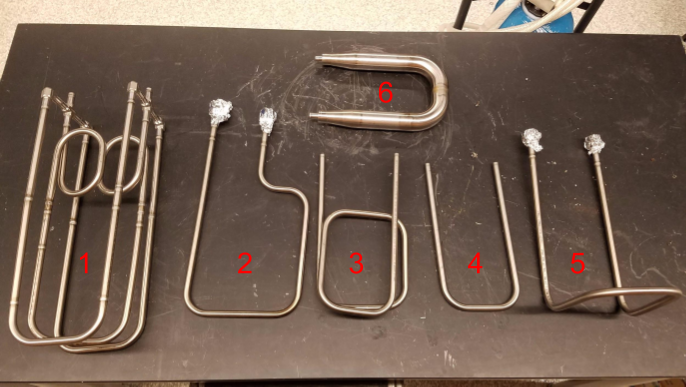
\includegraphics[width=\textwidth]{Figures/cold_trap_geometries.png}
\caption{Various cold trap geometries considered. We will refer to these geometries as follows: 1- Triple trap (0.5 inch). 2- Stocking trap. 3- Coil trap. 4- U trap (0.5 inch). 5- Boot trap. 6- U trap (1.5 inch). Not shown: 3/8 inch U trap. 1.5 inch triple trap. }
\label{fig:geometries}
\end{figure}

Moving on from the 1.5 inch U trap modifications, we decided to use 0.5 in plumbing in the construction of our traps. It sees about half of the krypton entrapment as the 1.5 inch trap and does not clog after $<10g$ of flow, as we found with the 3/8 inch trap. We did have some trouble with warm xenon gas breaking through to the output of the cold trap at higher flow rates. We welded a series of five traps with adding bends in the plumbing in order to increase the length of plumbing immersed in the LN. These traps are shown in \ref{fig:geometries}. We measure $\alpha$ for each of these cold traps, this time regulating the xenon flow with an MFC set to 3.3 SLM. 3.3 SLM is in the high-flow regime, so $\alpha$ will be decreased from the low-flow values. These measured values of $\alpha$ are shown in table \ref{tab:geo}. Refer to figure \ref{fig:geometries} for the description of the numbered cold traps. The results show that, while the additional bends do add more capacity to the trap, they can also reduce the krypton throughput.
\begin{table}
 \label{tab:geo}
 \begin{tabular}{c || c c c c c}
 \hline
 \hline
 Trap \# & 1 & 2 & 3 & 4 & 5 \\ [0.5ex] 
 \hline\hline
 $\alpha$ & 0.70 & 0.76 & 0.38 & 0.84 & 0.38 \\ [1ex] 
\hline
\end{tabular}
\caption{Throughput parameters measured for various cold trap geometries.}
\end{table}

Table \ref{tab:geo} indicates that trap \#2 has the best throughput apart from the U trap (trap 4\#). We have dubbed this the ``stocking trap" because of it's resemblance to a stocking, as well as because we first installed it on the system on Christmas, 2015. The stocking trap is capable of freezing about 120 grams of xenon before break-through, and only retains about 50\% more krypton than the 0.5 inch U trap. For the rest of this document, when we refer to ``the 0.5 inch diameter cold trap'', we will in fact be referencing the stocking trap, whereas when we refer to ``the 1.5 inch diameter cold trap'', we will be referring to the 1.5 inch U trap.


\subsection{Formation of Xenon Ice}
\label{sec:iceform}
The xenon ice forms in a short segment of plumbing relative to the approximately one foot length of the cold trap. The enthalpy of sublimation for xenon is about 15.95 kJ/mol at 77 kelvin.\cite{vaporpressure}. There is an additional 2.73 kJ/mol required to bring the xenon gas temperature down from 295 to 77 kelvin. A 0.36 SLM flow rate is equal to 0.267 mmol/sec of xenon, which requires 5.0 Watts to freeze. If we take the thermal conductance of stainless steel to be 10 W/m K, the maximum cooling power of a 12.7 mm diameter, 1.24 mm thick cold trap will be 70 W/mm. 

We must also consider the heat transfer from the LN to the stainless steel trap. The heat transfer rate from LN to a stainless steel surface is highly dependent upon the temperature difference between the bulk LN and the surface. This temperature dependance has a maximum, referred to as the critical heat flux, where the LN changes from ``nucleate boiling'' to ``film boiling''. Film boiling takes place when the LN boils rapidly enough to create an insulating layer, or ``film'', of nitrogen gas between the LN bath and the stainless steel surface. The critical heat flux of Stainless steel to LN is on the order of 10 W/cm$^2$, putting the maximum heat transfer to our 12.7 mm (0.5 inch) diameter cold trap at about 4 W/mm, making it the limiting factor in the heat transfer to the plumbing.\cite{LNheatflux} Similarly, a 1.5 inch diameter trap would have a heat transfer of about 12 W/mm, and a 0.25 inch trap would have a heat transfer of about 2 W/mm.

The above estimates of the heat transfer indicate that at flow rates $<1$ SLM, all of the xenon should be frozen within the first centimeter or so of cold plumbing. We can approximately measure the length of the ice-forming region in two ways. First, the length of this region is inferred by observing the bubble formation within the liquid nitrogen bath. As the xenon flow is frozen inside of the trap the heat is transferred to the LN bath, and the liquid nitrogen that is in contact with the ice forming region boils. In order to visually inspect the formation of xenon ice, we also installed a quartz window on the input and output of a cold trap. At low flow rates ($<1$ SLM), both of these methods indicate that the ice formation region is less than about 1 cm in length. When viewing the ice formation through a window, there is a clear collar of xenon ice that forms in the input side of the trap at the level of the LN bath, and there is no visible ice formation anywhere else. When observing the outside of the trap, the LN appears to boil where the plumbing enters the bath but nowhere else. In this low-flow regime, the ice collar will expand in depth as more xenon is added until it fully clogs the trap. Flowing at about 0.3 SLM, a 1.5 inch trap will clog after about 400g of xenon has been frozen, while a 0.5 inch trap will clog after only about 70g at 2 SLM.
\begin{figure}[h!]
\centering
\begin{subfigure}{0.45\textwidth}
  \centering
  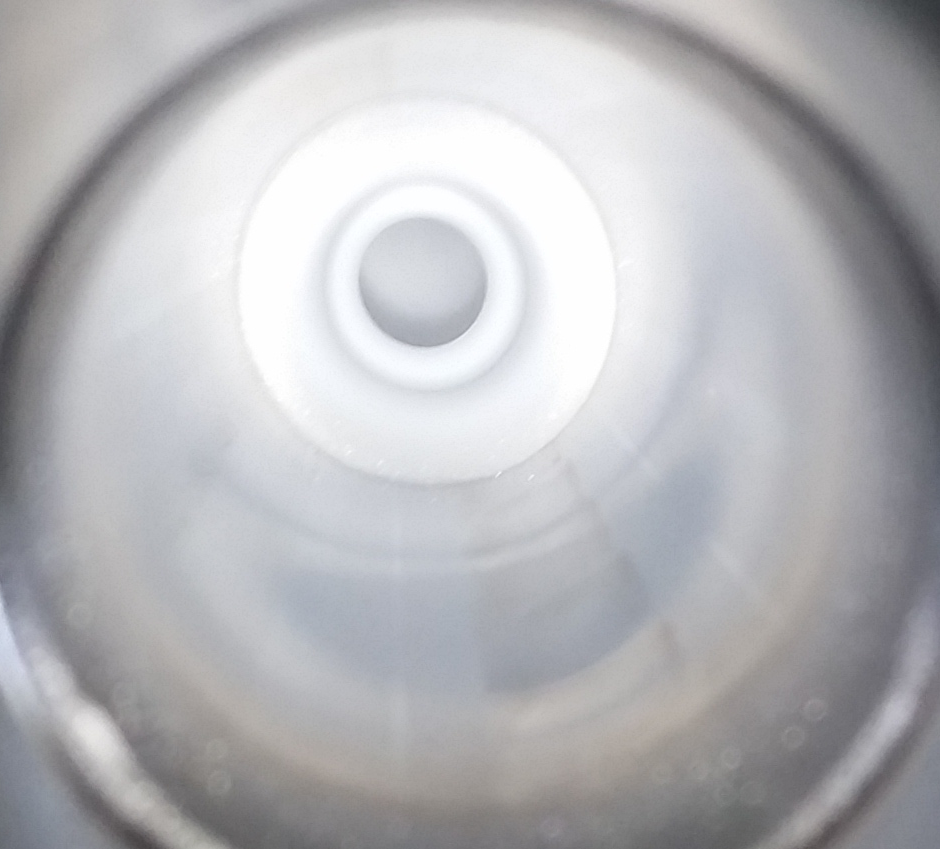
\includegraphics[width=\textwidth]{Figures/ice_plug_start.png}
  \caption{Ice collar forming.}
  \label{fig:plugstart}
\end{subfigure}\hfill%
\begin{subfigure}{0.45\textwidth}
  \centering
  \includegraphics[width=\textwidth]{Figures/ice_plug_full.png}
  \caption{Fully clogged trap}
  \label{fig:plugfull}
\end{subfigure}
\caption{Two images of how ice is formed in a cold trap. The left image shows a thick collar of ice beginning to form. This collar contains $>100$ grams of xenon ice. The right shows the collar after it has fully clogged the 1.5 inch diameter cold trap. This plug has roughly 400 grams of xenon is.} 
\label{fig:iceplug}
\end{figure}

At higher flow rates ($>1$ SLM), the ice no longer forms a collar, but rather a sleeve along the inside of the trap. This is likely due to the xenon ice forming an insulating layer over the stainless steel, thereby reducing the cooling power of that segment of plumbing to the point where it is no longer able to freeze the xenon. In the high flow regime, the LN will still only boil along a short segment of plumbing, but this segment can be seen to migrate along the trap from input to output. Eventually, enough of the trap surface is covered that the trap is no longer able to maintain a constant xenon temperature at the output and the xenon pressure at the RGA rises. We call this effect xenon break-through, and is avoided whenever possible. The xenon pressure is already set to be higher than the operational pressure of the RGA, so any significant increase above this set-point could cause damage to the RGA. Additionally, either from physical effects inside the cold trap or from electronics effects of the RGA becoming over-pressured, $PP_{Kr}$ tends to drop in the xenon break-through region limiting the usefulness of any data taken in the region.
\begin{figure}[h!]
\centering
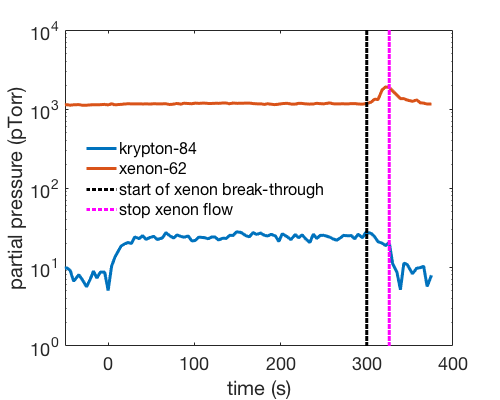
\includegraphics[width=\textwidth]{Figures/xenon_breakthrough.png}
\caption{Break-through of xenon to the RGA, through a 0.5 inch trap. 4 SLM xenon flow was started at t=0 seconds, and xenon breakthrough occurred $300\pm5$ seconds later. This means that about 120 grams of xenon ice formed before flow was shut off; approximately double the amount in an ice plug formed in the low flow regime.}
\label{fig:breakthrough}
\end{figure} 

In addition to the considerations from actively forming xenon ice, there are also issues and dependencies that arise from ice that was formed in the cold trap prior to beginning flow. In the high-pressure in which we operate the RGA, the RGA electronic baseline offset is highly dependent on the pressure of xenon. This means we need the xenon pressure to be extremely stable over the course of the xenon flow, otherwise we may see a false krypton signal caused by a rising electronic offset. To this end, we must form a small kernel of ice prior to an analysis run so that once xenon flow starts the electronic baseline at at xenon ice pressure will already have been established. 

To see the possible effects of failing to maintain a stable xenon pressure we look to figure \ref{fig:correlatednoise}. In looking for a genuine krypton signal, we can check that the mass abundances are correct. The 84 amu line should be roughly 3 times more prominent than the 83 amu line. Additionally, there should be no pressure at 87 amu, so this line will be a good tracer for the baseline offset. For the purposes of this plot, we do a standard normalization ($P_{norm}=\frac{P-\mu}{\sigma}$) on all four pressure traces In order to put them on the same scale. The xenon pressure was not well controlled for this run and rose by roughly 2 $\sigma$ when the flow was started. We also saw a corresponding 2-$\sigma$ rise in both of the krypton traces as well as the 87 amu baseline-tracker line. The rise in the krypton lines are clearly not genuine, but rather an artifact of a shifting electronic baseline offset. These false signals are extremely dangerous in that that can mimic a genuine signal in excess of 10 times our limit of sensitivity. To insulate ourselves against this possibility, we always track multiple krypton masses, and use their signal ratios as a quality check. We also track a baseline tracer such as 87 amu and xenon pressure. If either of these has a statistically significant rise during the analysis run we mark the measurement as untrustworthy.
\begin{figure}[h!]
\centering
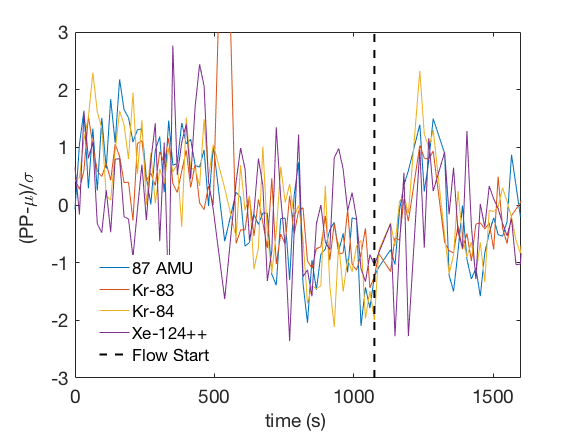
\includegraphics[width=\textwidth]{Figures/RGA_noise_correlation.png}
\caption{Data from an analysis run with poorly controlled xenon pressure. The krypton-83 and -84 lines, as well as a baseline tracer at 87 amu all tracked the drifting xenon pressure exactly. } 
\label{fig:correlatednoise}
\end{figure} 

We maintain xenon pressure during an analysis run by forming an initial kernel of ice, onto which the the rest of the xenon will be frozen. The way this kernel is distributed through the trap has some effects on the response of the trap. We examine three methods of forming the ice kernel, along with their impacts of the ultimate sensitivity of the system. 

We begin with the simplest method of forming an ice kernel. We inject roughly 10 standard cc's of xenon into the input of the trap in order to form the base of the ice collar. This procedure does not, however, adequately maintain xenon pressure during xenon flow. When we flow xenon at a rate of 2.5 SLM, we see a rise in both the electronic baseline and the xenon partial pressure of, on average, 4.2-$\sigma$. By dumping xenon into the ice collar, we are increasing the temperature of the collar, and therefore are increasing the vapor pressure above it. We might expect that this high-vapor pressure xenon will be frozen at some point further along the trap, thereby maintaining the pressure at the output. However, this xenon elevated xenon pressure seems to be low enough that it will not readily freeze to the cold stainless steel of the trap, and will maintain its elevated pressure all the way through the trap.

To prevent the xenon vapor pressure from rising, we modify our kernel formation technique in order to provide nucleation points for sublimation in the middle and output of the cold trap. We do this by filling the warm cold trap with the full sample pressure of xenon, usually about 2,000 Torr. We the isolate the trap and immerse it in the LN bath allowing this 2,000 Torr of xenon to freeze along the full length of the immersed plumbing. We then add an output kernel by injecting about 10 standard cc into the output of the trap, through V5. Using this method of kernel formation prior to flowing at 2.5 SLM, the change in xenon pressure and baseline offset are reduced to an average of $-0.85-\sigma$. 

Although this method appears to be successful in eliminating, it bring with it two problems. The first problem is that as the LN bath evaporates, the height of the bath may lower below the output kernel. If this happens, the xenon partial pressure at the RGA will rise, leading to a rising baseline. To counter, this we form the kernel with the trap not yet fully submerged in the bath. Once the kernel has been formed, we immerse the trap the rest of the way.

The second problem with this modified technique is that the ice sleeve can interfere with the krypton throughput, thereby reducing $PP_{Kr}$. This seems to only occur if a large enough amount of xenon (~500 standard cc) is used in the formation of the kernel. If we use only about 50 standard cc of xenon, this effect seems to go away without loss in baseline stability. 
\begin{figure}[h!]
\centering
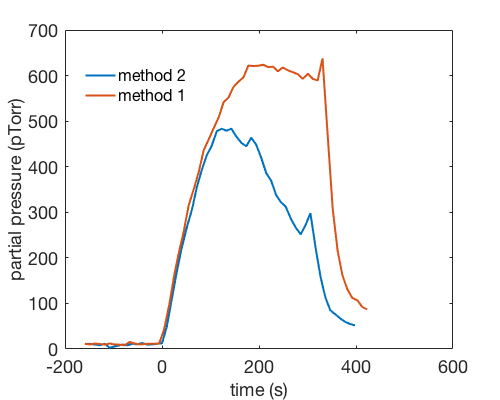
\includegraphics[width=\textwidth]{Figures/ice_form_Krloss.png}
\caption{Krypton trace using the initial and modified method's prior to 2.5 SLM xenon flow, and a 90x impedance setting. For the method 2 trace we used ~2500 Torr (600 standard cc) to for the kernel. This trace begins on the trend as method 1, but sees a sharp turn over and maxes out at only 63\% of the method 1 peak. } 
\label{fig:iceformkrloss}
\end{figure} 


\subsection{Flow Rate Dependance}
\label{sec:flow_real}
As mentioned previously, there are two distinct regimes of xenon flow in a cold trap sampling system: the low flow regime in which all of the xenon ice is formed within millimeters of the LN surface level, and the high flow regime in which the xenon ice forms a sleeve, which eventually can reach the output side of the trap and cause the RGA xenon pressure to rise. In the low flow regime, the response of the sold trap system to flow rate is extremely linear. In the high flow regime this linearity breaks down. As the ice sleeve rounds bends in the trap the interaction between the krypton flow and the xenon ice formation changes. These changes work to lower the krypton pressure at the RGA from the exponential response predicted in equation \ref{eq:CTresponse}, as can be seen in figure \ref{fig:KrDrop}.

\begin{figure}[h!]
\centering
\begin{subfigure}{0.5\textwidth}
  \centering
  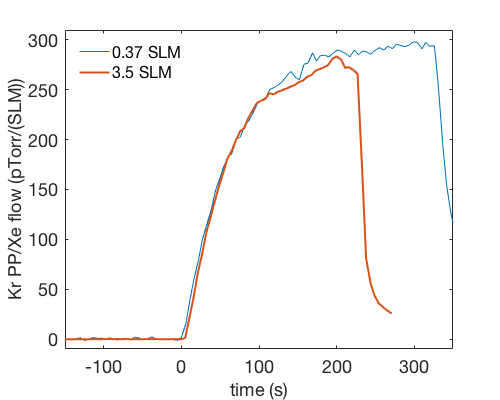
\includegraphics[width=\textwidth]{Figures/SLAC_flow_turnover.png}
  \caption{0.5 inch trap.}
  \label{fig:KrDrop0p5}
\end{subfigure}%
\begin{subfigure}{0.5\textwidth}
  \centering
  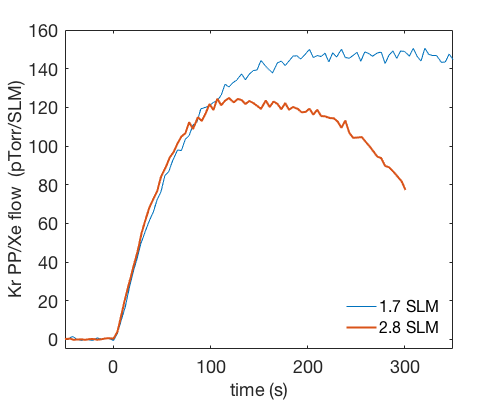
\includegraphics[width=\textwidth]{Figures/SLAC_flow_turnover_1p5in.png}
  \caption{1.5 inch trap.}
  \label{fig:KrDrop1p5}
\end{subfigure}
\caption{Krypton pressure traces resulting from high and low xenon flow regimes. Note the two sharp kinks in the 0.5 inch trend. These correspond to sharp 90-degree bends in the tubing of the trap which were formed using a standard tube-bender. The rounded turns in the 1.5 inch trend correspond to the more gentle bends in the 1.5 inch tubing. These bends are built by welding two elbow pieces together. These measurements were taken in the 15x impedance state.} 
\label{fig:KrDrop}
\end{figure}

We do not have a satisfactory explanation as to the physical basis of this drop in krypton pressure at the RGA. Speculations could be made, but in the end we are only interested in how this phenomenon will affect our sensitivity to krypton. To characterize the impacts that flow rate has on the krypton response, we run tests at various flow rates and track the maximum pressure the krypton trace reaches at each setting. We also repeated this flow-rate scan for several impedance states. Above about 2 SLM, the turn-over effect shown in figure \ref{fig:KrDrop} begins competing with the idealized response described in equation \ref{eq:CTresponse}. This effect is more pronounced at higher impedance settings, but can be clearly seen even in the 1x impedance scan above about 6 SLM.
\begin{figure}[h!]
\centering
\begin{subfigure}{0.5\textwidth}
  \centering
  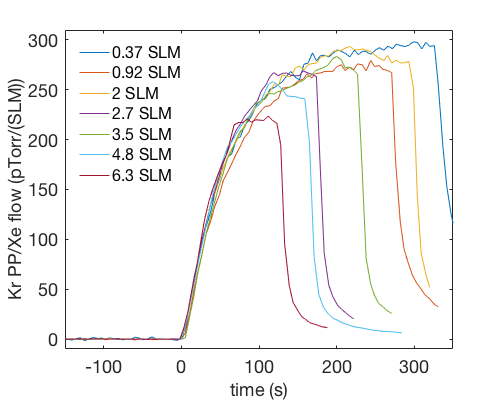
\includegraphics[width=\textwidth]{Figures/SLAC_FlowResponse_15x.png}
  \caption{0.5 inch trap.}
  \label{fig:flow_traces_0p5}
\end{subfigure}%
\begin{subfigure}{0.5\textwidth}
  \centering
  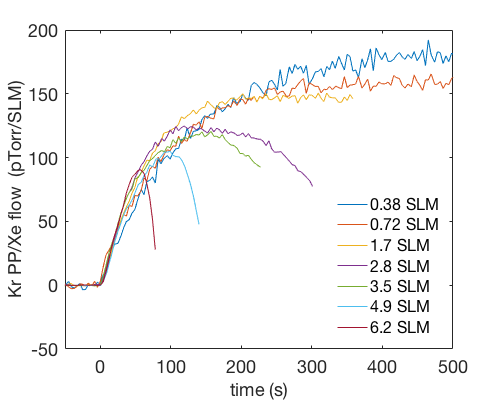
\includegraphics[width=\textwidth]{Figures/SLAC_FlowResponse_15x_1p5in.png}
  \caption{1.5 inch trap.}
  \label{fig:flow_traces_1p5}
\end{subfigure}
\caption{Krypton RGA traces normalized to xenon flow rate at various flow rate settings. These traces are all measurements of identical xenon, with an impedance setting of 15x. The response of the system to flow rate appears to be largely linear until about 2 SLM. After this point the Kr trace falls increasingly down from the low-flow traces.} 
\label{fig:flow_traces}
\end{figure}
\begin{figure}[h]
  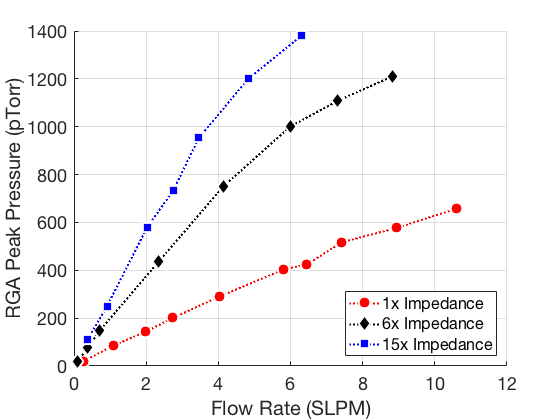
\includegraphics[width=\linewidth]{Figures/FlowResponse.png}
  \caption{Peak krypton RGA pressure as a function of flow rate, and at varying impedance settings. The data for this plot was taken with a 0.5 inch diameter cold trap.}
  \label{fig:RGAtrace_ideal}
\end{figure}

The turn-over effect is so dominant in the flow rate dependence of $\alpha$, that it obscures other possible effects. The usual method of calculating the equilibrium krypton pressure, $PP_{Kr,eq}$ is to flow xenon until $PP_{Kr}(t)$ levels off to a constant value. The data in this constant region is then averaged to find $PP_{Kr,eq}$. However, the turn-over effect can create a false plateau in the $PP_{Kr}(t)$ data which invalidates this flat-top averaging method. To account for this effect we can look only at the portion of $PP_{Kr}(t)$ before the first turn-over. This will be data from the time when ice is forming only in the first segment of the cold trap, before the ice sleeve grows around the first bend. If we fit the  exponential response from equation \ref{eq:CTresponse} to this first segment of $PP_{Kr}(t)$, we can estimate what $PP_{Kr,eq}$ would be without the turnover effect.
\begin{figure}[h]
  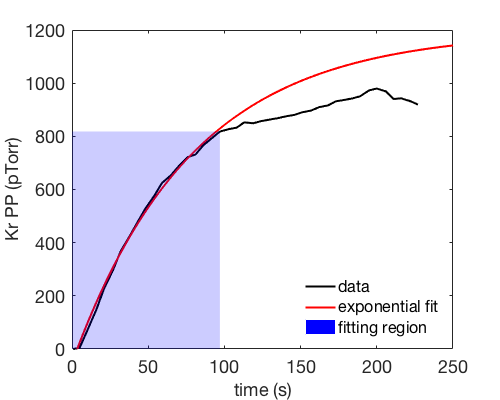
\includegraphics[width=\linewidth]{Figures/turn_over.png}
  \caption{An example of fitting an exponential response to the first part of $PP_{Kr}(t)$. This is the same data plotted in figure \ref{fig:KrDrop0p5}}
  \label{fig:turn_over}
\end{figure}

At low flow rates, the extrapolated values of $PP_{Kr,eq}$ are equal to the flat-top averages. This is expected, since the xenon flow is in the regime where all of the ice is formed in the first leg of the trap, and the turn-over effect does not come into play. At higher flow rates, when the turn-over effect begins to turn on, the two $PP_{Kr,eq}$ values begin to diverge. The exponential fit values continue on a linear trend, while the flat top averages fall off of this linear trend. Returning to equation \ref{eq:krpres2} we see that $PP_{Kr,eq}$ can only remain linear with flow rate if $\alpha$ has no flow rate dependence. From the fact that the exponential fit values do remain linear, we conclude that $\alpha$ is not inherently affected by xenon flow rate, but rather picks up an effective flow rate dependence because of the turn-over effect.
\begin{figure}[h!]
\centering
\begin{subfigure}{0.5\textwidth}
  \centering
  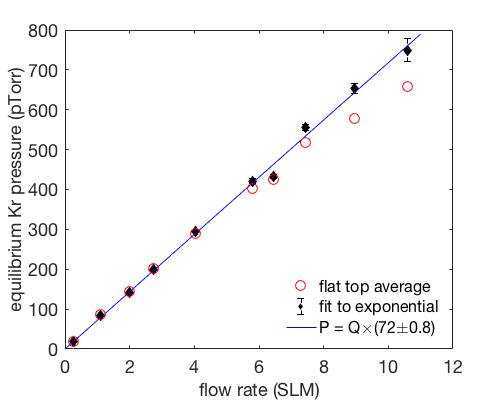
\includegraphics[width=\textwidth]{Figures/SLAC_FlowResponse_1x_linfit.png}
  \caption{1x impedance.}
  \label{fig:flowresponse1x}
\end{subfigure}%
\begin{subfigure}{0.5\textwidth}
  \centering
  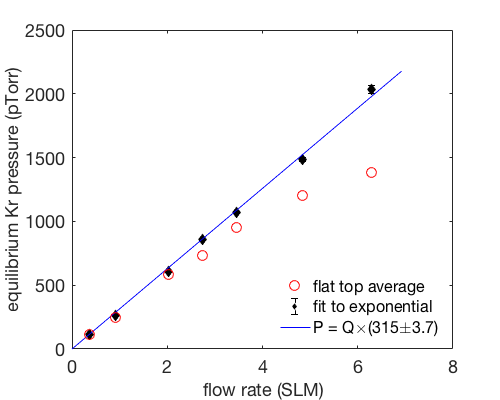
\includegraphics[width=\textwidth]{Figures/SLAC_FlowResponse_15x_linplot.png}
  \caption{15x impedance.}
  \label{fig:flowresponse_15x}
\end{subfigure}
\caption{Comparison of the flat-top averaged $PP_{Kr,eq}$ the extrapolated equilibrium value calculated from a fit to an exponential response.} 
\label{fig:flowresponse}
\end{figure}



\subsection{Impedance Dependance}
\label{sec:impedance_real}
The predictions of equation \ref{eq:CTresponse} also break down at high system impedances, although perhaps in a more well-behaved way than in the case of high xenon flow rates. Just as with increased xenon flow rate, the $\alpha$ parameter will increase at higher impedance settings. However, as opposed to its turn-over induced, effective dependence on flow rate, $\alpha$ appears to have a more fundamental relation to impedance that can be used to characterize the physical basis of the entrapment of krypton in the cold trap.

Consider the pressure trace shown in figure \ref{fig:RGAtrace_slow}; the xenon flow rate, $Q_0$ and krypton concentration, $\Phi$ were identical to the krypton trace in figure \ref{fig:RGAtrace_fast}, and the impedance, $Z_1$ was set to be 45 time higher. This trace deviates significantly from what would be expected by increasing $Z_1$ in equation \ref{fig:CTresponse}. Both the system response time and equilibrium pressure are expected to increase proportional to $Z_1$ from equations \ref{eq:CTtime} and \ref{eq:krpres2}, but had a significantly smaller increase. $PP_{Kr,eq}$ increased from $50.8 \pm 0.4$ to $399.9\pm 1.7$ pTorr; a factor of 7.9. The overall response time, $\tau$, increased from $12.7 \pm 0.7$ to $93.4 \pm 1.8$ seconds; a factor of 7.4. 
\begin{figure}[h!]
\centering
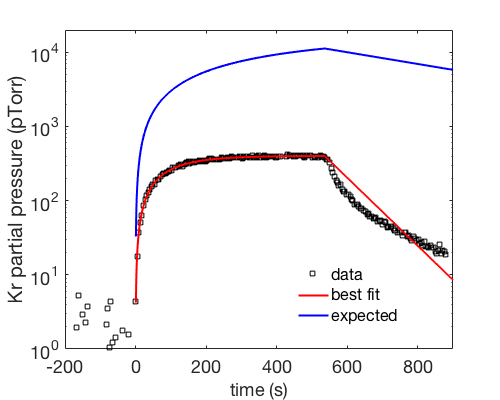
\includegraphics[width=\textwidth]{Figures/RGAtrace_fit_slow_wexp.png}
\caption{RGA trace with 45x impedance settings. }
\label{fig:RGAtrace_slow}
\end{figure}

It is an interesting point of fact that the discrepancy in both $PP_{Kr,eq}$ and $\tau$ from the predicted results are approximately the same. In fact, although $PP_{Kr,eq}$ and $\tau$ no not remain proportional to $Z_1$, they do remain proportional to each other. One explanation for this would be that our measurements of $Z_1$ and $S_{RGA}$ are incorrect, and the impedances are not being increased as much as we have calculated. However, this would only satisfy the proportionality of $PP_{Kr,eq}$ and $\tau$ if the throughput parameter, $\alpha$ is constant with impedance. 
\begin{figure}[h!]
\centering
\begin{subfigure}{0.5\textwidth}
  \centering
  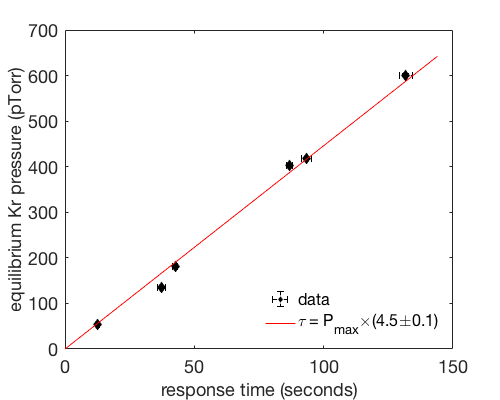
\includegraphics[width=\textwidth]{Figures/SLAC_imp_response_linfit.png}
  \caption{0.5 inch trap}
\end{subfigure}%
\begin{subfigure}{0.5\textwidth}
  \centering
  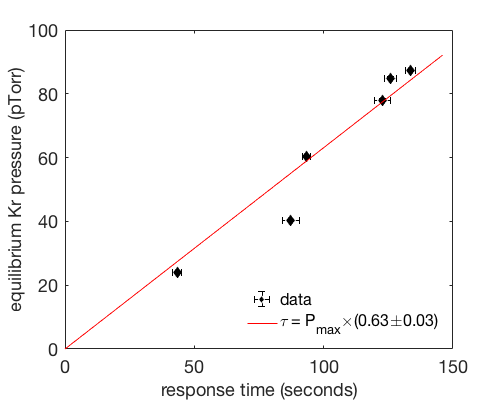
\includegraphics[width=\textwidth]{Figures/SLAC_imp_response_1p5in_linfit.png}
  \caption{1.5 inch trap}
\end{subfigure}
\caption{Linearity of the characteristic response time, $\tau$, and the equilibrium krypton pressure, $PP_{Kr,eq}$.} 
\label{fig:impresponse_lin}
\end{figure}

In order to measure $\alpha$, we can measure the concentration of krypton in xenon which is left over from an analysis. After flowing a sample into the cold trap for analysis, the sample bottle will be left empty, and all of the xenon (minus a microscopic amount that gets pumped out past the RGA) will be frozen in the cold trap. Along with this frozen xenon will be the krypton that was trapped. We can then transfer this new mixture back into the sample bottle and run a second pass analysis. The ratio of $PP_{Kr,eq}$  from the second pass to the first pass will be equal to the fraction of krypton which gets trapped in the cold trap. This ratio will also be equal to 1-$\overline{\alpha}$. It may be that the throughput parameter during the transient rising section of $PP_{Kr}(t)$ will be different from the equilibrium value. In this case, the averaged $\overline{\alpha}$ will differ from the equilibrium value of $\alpha$ which is presented in section \ref{sec:response}. 

Measurements of $\overline{\alpha}$ over a series of impedance settings show that the throughput is decreasing at higher impedances. This means that the fact that $PP_{Kr,eq}$ is not linear in $Z_1$, as is predicted be equation \ref{eq:CTresponse}, cannot be fully explained by faulty impedances measurements.
\begin{figure}[h!]
\centering
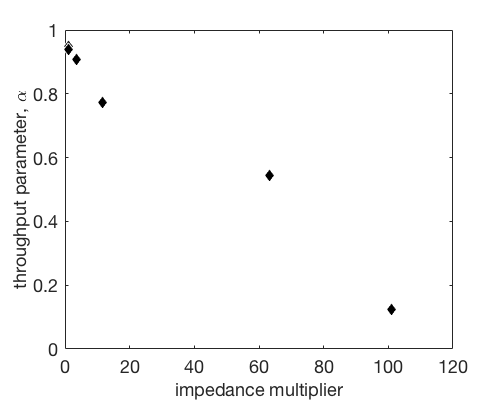
\includegraphics[width=\textwidth]{Figures/SLAC_alpha.png}
\caption{Left-over method of calculating $\overline{\alpha}$. The decreasing trend in the throughput indicates that error in the impedance measurements cannot fully explain the observed deviation from equation \ref{eq:CTresponse}. }
\label{fig:alpha}
\end{figure}

Now that we have established that the krypton throughput is reduced at higher impedances, we return to our idealized model from section \ref{sec:response} and attempt to incorporate a finite throughput into our equations. For simplicity, we will make the assumption that the pressure in the RGA volume responds instantaneously to the pressure in the cold trap volume ($P_{Kr,CT}$), so at any moment, $t$, $PP_{Kr}(t)=P_{Kr,CT}(t)/180$. We start by rebuilding the differential equation for $P_{Kr,CT}(t)$ this time adding a term for entrapment:
\begin{equation}
\label{eq:expdiff2}
V\frac{dP_{Kr,CT}}{dt}=\Phi Q_{Xe,CT}(t)-P_{Kr,CT}(t)/Z_1-Q_{trap}(t),
\end{equation}
where $Q_{trap}(t)$ represents the rate at which krypton is becoming trapped in the xenon ice at a given time. In the constant flow, equilibrium limit we can write $Q_{trap}$ in terms of $\alpha$:
\begin{equation}
P_{Kr,CT}/Z_1= \Phi Q_{Xe,CT}-Q_{trap}=\alpha \Phi Q_{Xe,CT},
\end{equation}
which can be rewritten:
\begin{equation}
Q_{trap}=(1-\alpha )\Phi Q_{Xe,CT}=(\frac{1}{\alpha}-1)P_{Kr,CT}/Z_1.
\end{equation}
We do not know a priori how $\alpha$ and $Q_{trap}$ will behave in the non-equilibrium case. The simplest assumption to make is that $\alpha$ remains constant over the full time range in which xenon is flowing. In this case the entrapment rate, entrapment rate takes the form of a virtual leak with constant volumetric pumping rate: 
\begin{equation}
Q_{trap}(t) = S_{trap}P_{Kr,CT}(t),
\end{equation}
where,
\begin{equation}
\label{eq:strap}
S_{trap}=\frac{1}{Z_1}(\frac{1}{\alpha}-1).
\end{equation}
Rewriting equation \ref{eq:expdiff2} with this assumption we get a new exponential response equation for $P_{Kr,CT}(t)$:
\begin{align}
 \label{eq:expdiff3}
V\frac{dP_{Kr,CT}}{dt}&=\Phi Q_{Xe,CT}(t)-(\frac{1}{Z_1}+\frac{1}{Z_1}(\frac{1}{\alpha}-1))P_{Kr,CT}(t)\\
&=\Phi Q_{Xe,CT}(t)-\frac{1}{\alpha Z_1}P_{Kr,CT}(t)
\end{align}

After accounting for a constant throughput parameter, the overall response time constant of the cold trap will have a linear dependance on the throughput parameter:
\begin{equation}
\label{eq:tau_alpha}
\tau=\alpha Z_1 V.
\end{equation}
This agrees with the linearity between $\tau$ and $PP_{Kr,eq}$ shown in figure \ref{fig:impresponse_lin}. To make this explicit, we can use equation \ref{eq:tau_alpha} to rewrite equation \ref{eq:krpres2}:
\begin{equation}
\label{eq:krpres3}
PP_{Kr,eq}=\frac{\tau}{180V}Q_{Xe,CT}\Phi_{Kr}.
\end{equation}

A further assumption we could make is that $S_{trap}$ does not have a dependence on $Z_1$. Under this assumption, we can begin to make predictions about how $\alpha$ will behave as a function of impedance. Writing equation \ref{eq:expdiff3} in terms of $S_{trap}$ gives:
\begin{equation}
V\frac{dP_{Kr,CT}}{dt}=\Phi Q_{Xe,CT}(t)-(\frac{1}{Z_1}+S_{trap})P_{Kr,CT}(t),
\end{equation}
which means:
\begin{align}
\label{eq:tau_s}
\frac{1}{\tau}&=\frac{1}{Z_1 V}+\frac{S_{trap}}{V}\\
\tau&=V\frac{Z_1}{1+Z_1S_{trap}}
\end{align}
Another way to put this is that the overall response time is the inverse sum of the idealized output time constant, and the entrapment time constant:
\begin{equation}
\label{eq:tau_sum}
\frac{1}{\tau}=\frac{1}{\tau_{out}}+\frac{1}{\tau_{trap}},
\end{equation}
where $\tau_{out}=Z_1V$ and $\tau_{trap}=V/S_{trap}$. Equation \ref{eq:tau_sum} indicates that when $\tau_{out}<<\tau_{trap}$ the cold trap response will have the idealized linear dependance on $Z_1$. However, in the limit $\tau_{out}>>\tau_{trap}$, the response will approach a constant in $Z_1$.

Substituting equation \ref{eq:tau_s} into equation \ref{eq:krpres3}, we get:
\begin{equation}
\label{eq:krpres4}
PP_{Kr,eq}=\frac{1}{180}Q_{Xe,CT}\Phi_{Kr}\frac{Z_1}{1+S_{trap}Z_1}.
\end{equation}
We fit this equation to the $PP_{Kr,eq}$ data taken at various impedance settings. We approximate the corresponding $Z_1$ values in the following way. We calculate $Z_1$ at the 1x impedance setting using equation \ref{eq:tau_alpha}, where $\tau$ is the best fit value to $PP_{Kr}(t)$, and $\alpha$ is measured using the left-over method. The rest of the $Z_1$ values are calculated by multiplying the 1x impedance value by the scaling factor measured in the adjustment of the xenon pressure described in section \ref{sec:imp_set}. For the 0.5 inch trap, we take $V=183.8$ cc. For the 1.5 inch trap, we did not measure the volume, so assume that $Z_1$ at 1x impedance is the same for both traps.

The data for $Z_1$ versus $PP_{Kr,eq}$ fits reasonably well to equation \ref{eq:krpres4}. For the 0.5 inch trap, the best fit $S_{trap}$ =0.89 $\pm$0.12 cc/s and $\tau_{trap}$ = 207 $\pm$30 s. For the 1.5 inch trap, $S_{trap}$ =2.6 $\pm$0.5 cc/s and $\tau_{trap}$ = 180 $\pm$30 s.
\begin{figure}[h!]
\centering
\begin{subfigure}{0.5\textwidth}
  \centering
  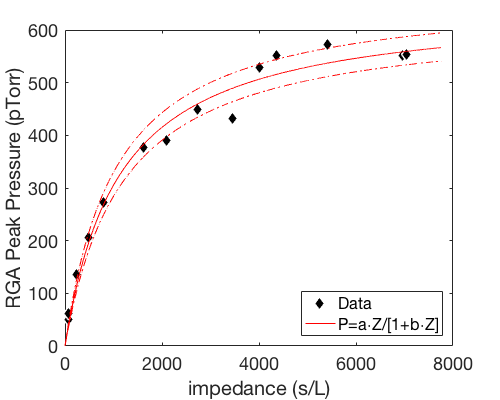
\includegraphics[width=\textwidth]{Figures/SLAC_imp_response.png}
  \caption{0.5 inch trap}
\end{subfigure}%
\begin{subfigure}{0.5\textwidth}
  \centering
  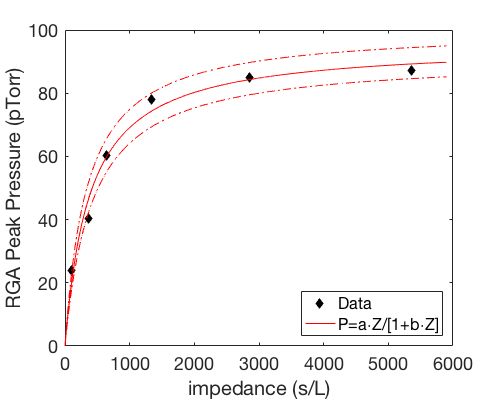
\includegraphics[width=\textwidth]{Figures/SLAC_imp_response_1p5in.png}
  \caption{1.5 inch trap}
\end{subfigure}
\caption{Equilibrium krypton pressure as a function of impedance. This fitting model is derived from the assumption that $S_{trap}$ is independent of impedance. The data fits this model reasonably well.} 
\label{fig:impresponse}
\end{figure}

\subsection{Post Flow Behavior}
To this point we have largely ignored the behavior of $PP_{Kr}(t)$ after the xenon flow has been stopped, but this data contains interesting features that are worth investigating. The most obvious feature is the departure from the exponential decay expected from equation \ref{eq:CTresponse}. In figure \ref{fig:RGAtrace_slow} we see that after the flow is turned off, the krypton pressure begins to drop much faster than the trend expected from the fit to the rising portion ($\tau_{rise}$) but turns over and eventually levels of to an exponential trend with a significantly longer time constant than expected. 

Our best explanation for the quickly falling transient behavior is that the volume of the cold trap becoming effectively larger when the flow is turned off. While a macroscopic amount of xenon is being flowed into the cold trap, the input side of the cold trap will not be in equilibrium with the output side. As mentioned previously, the input side of the cold trap will be in viscous flow, while the output will be near vacuum. In this arrangement, the krypton pressure in the vacuum state ($P_{Kr,CT}$) will be physically restricted from expanding past the ice-forming region, effectively reducing the volume of the cold trap. Once flow has stopped, this molecular-flow krypton will be allowed to expand into the full cold-trap volume, and in so doing, will lower $P_{Kr,CT}$. To confirm this effect, we conduct two trials with identical impedance, flow rate, and sample mass. In the first trial we use a 502cc, 0.5 inch diameter cold trap. In the second test, we add a 500cc stainless steel sample bottle to the output of the trap. Since the sample bottle is already in the vacuum state before the xenon flow is turned off, the volume difference should be much smaller, and therefore the transient drop should be much smaller. 
\begin{figure}[h!]
\centering
\begin{subfigure}{0.5\textwidth}
  \centering
  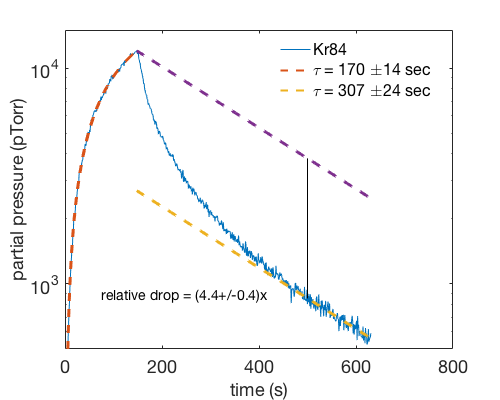
\includegraphics[width=\textwidth]{Figures/post_flow_transient_nobottle.png}
  \caption{without 500cc bottle}
\end{subfigure}%
\begin{subfigure}{0.5\textwidth}
  \centering
  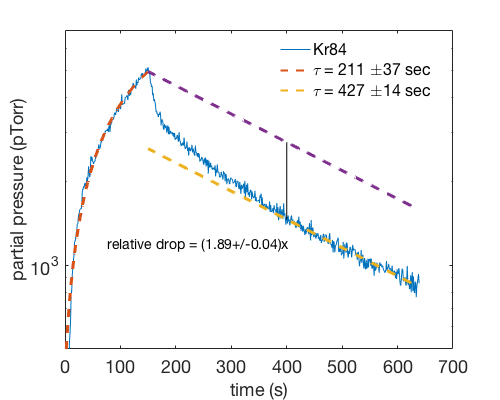
\includegraphics[width=\textwidth]{Figures/post_flow_transient_wbottle.png}
  \caption{With 500cc bottle}
\end{subfigure}
\caption{Trials with and without a 500cc sample bottle connected to the output of the cold trap. These runs were both done at 3SLM, and at 19x impedance.} 
\label{fig:transientdrop}
\end{figure}

After running these trials at 3SLM and 19x impedance, we find that when the 500cc bottle is attached, $P_{Kr,CT}$ drops by $(47\pm1)$\% in the transient region. When the bottle is not connected, this drop is $(77\pm2)$\%. We calculate these drops by fitting an exponential decay to the region of $P_{Kr,CT}(t)$ after it has leveled off from the transient region. We then take the difference between this trend and a trend with the same time constant which passes through the last point of $P_{Kr,CT}$ before the xenon flow was stopped. It should also be noted here that the rise time and fall time are both longer in the trial with the bottle attached, but not as much as might be expected from doubling the cold trap volume. In fact, the rise times are only about 1 standard deviation apart. It may be that the added impedance of the valve used to connect the bottle to the cold trap limits communication between the two volumes. Also, we ran these trials in the high xenon flow regime in which the ice formation region will move along the length of the cold trap over the course of the run. This should make the effective volume increase more pronounced but may obscure tests pertaining to the rise and fall time constants.

We also used the post flow region of the data to test whether or not there was diffusion occurring in the cold trap. We ran several tests in which we would close V6 in order to shut off the $P/Z_1$ term in equation \ref{eq:expdiff3}. In this way we hoped to measure the rate at which $P_{Kr,CT}$ is reduced purely by diffusion into static xenon ice. 
\begin{figure}[h!]
\centering
\begin{subfigure}{0.5\textwidth}
  \centering
  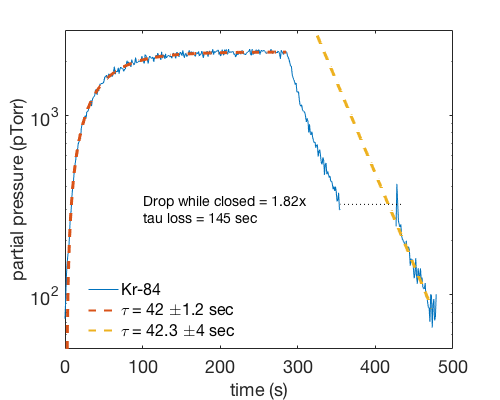
\includegraphics[width=\textwidth]{Figures/cyrano_pvt_1x.png}
  \caption{1x impedance}
  \label{fig:cyrano1x}
\end{subfigure}%
\begin{subfigure}{0.5\textwidth}
  \centering
  \includegraphics[width=\textwidth]{Figures/cyrano_pvt_15x.png}
  \caption{19x impedance}
  \label{fig:cyrano15x}
\end{subfigure}
\caption{Trials at 1x and 19x impedance, each at 0.3 SLM. Each trial has a period of time during post-flow in which V6 was closed; a 70 second period in the 1x case and a 210 second period in the 19x case. In both trials, the fractional drop in pressure while V6 was close was was roughly the same. The post-flow transient drop was calculated to be ($26\pm10$)\% for the 1x impedance run and ($34\pm8$)\% for the 19x impedance run. The ``tau loss'' indicated on the plots are extrapolated time constants assuming the pressure drop with V6 closed is due to some exponential decay.} 
\label{fig:cyrano_trace}
\end{figure}

The results were somewhat ambiguous; we did find that the krypton pressure dropped while V6 was closed, but the fractional drop was on the order of about $(1.7\pm0.2)$ regardless of the amount of time V6 was left closed ($\Delta t$). This is more indicative of a separate issue having to do with the process of closing and reopening V6 than it is of diffusion. We would expect that more krypton would diffuse into the ice the longer it was left in this static state. We chose longer $\Delta t$'s to correspond to higher impedances. It is possible that there was an impedance-dependent diffusion which our choice of $\Delta t$ happened to cancel out, however an impedance-dependent diffusion would disagree with the results from the previous section.
\begin{figure}[h!]
\centering
\includegraphics[width=\textwidth]{Figures/diffusion_pdrop.png}
\caption{Lost krypton pressure as a function of the length of time with V6 closed. There does not seem to be a clear trend. }
\label{fig:closed_drop}
\end{figure}

The question remains as to why the long term post-flow decay rate of $P_{Kr,CT}(t)$ is so much lower than the best-fit rate of the rising data. The obvious answer would be in $\tau$'s proportionality to the volume of the cold trap. If $V$ sees an effective increase after the xenon flow is turned off, then $\tau$ would see an increase of the same relative size. This matches the data from figure \ref{fig:cyrano15x} in which the fractional increase in $\tau$ is $1.4\pm0.3$, and the fractional increase in volume calculated from the post-flow transient drop in pressure is $1.5\pm0.2$. 

There is still some tension with the data. First, we don't see a post-flow change in $\tau$ in the 1x impedance plot (figure \ref{fig:cyrano1x}) like we see in the 19x impedance plot. Also, we see no clear evidence of krypton entrapment occurring when the xenon flow has been turned off, leaving only entrainment-like effects. These should turn off in the post flow region, allowing $\tau$ to approach its predicted value. In the case of figure \ref{fig:cyrano15x}, the expected value is approximately $1.4\times19\times 42$ sec $=1120$ sec after accounting for the impedance factor and effective volume increase. Instead, we see no evidence of this turn-off at all.


\subsection{Diffusion and Entrainment}
In the previous sections we constructed a model where the krypton entrapment rate behaves in the manner of a constant volumetric pumping speed. This model provides a decent representation of the data, but we are left to ask what this model can tell us about the physical source of the entrapment. We have two postulations as to the source of krypton entrapment; diffusion and entrainment. 

Diffusion is governed by two equations- Fick's two laws of diffusion. In one dimension, these are:
\begin{equation} \label{eq:fick1}
J = -\frac{d\phi}{dx}
\end{equation}
\begin{equation}\label{eq:fick2}
{\partial \phi \over \partial t} = D \frac{\partial ^{2} \phi}{\partial x ^2}
\end{equation}
Here $J$ is the amount of substance per unit area per unit time, $D$ is the diffusion coefficient, and $\phi$ is the concentration of krypton at a certain depth, $x$, and certain time, $t$. The boundary concentration at $x=0$ will be given by the pressure of krypton above the ice and the solubility constant, $K$:
\begin{equation}
\phi(0,t)=P_{Kr,CT}(t)K
\end{equation}
We can then use equation \ref{eq:fick1} to write the entrapment rate of krypton due to diffusion:
\begin{equation}
Q_{diffusion}(t)=-AD\frac{d\phi}{dx}(x=0,t),
\end{equation}
where $A$ is the surface are of xenon ice.

To get an idea for the time dependence of the diffusion rate, we'll consider the simplified case of a constant $P_{Kr,CT}$above a static sheet of unchanging thickness, $L$, and surface area, $A$. Diffusion in this scenario could fall into two regimes. for large values of D, the krypton will penetrate quickly, the ice will approach saturation, and the boundary conditions will be $\phi(x>0,t=0)=0$, $\phi(x=0,t)=P_{Kr,CT}K$, and $\frac{\partial \phi}{\partial x} (x=L,t)=0$. In this regime, equation \ref{eq:fick2} can be solved using a Fourier series of a rectangular wave with wavelength of $4L$, height of $-P_{Kr,CT}K$, and DC offset of $P_{Kr,CT}K$:
\begin{equation}
\phi(x,t=0)=P_{Kr,CT}K[1-\frac{4}{\pi}\sum_{n_{odd}}\frac{sin(\frac{n\pi x}{2L})}{n}].
\end{equation}
After we feed this series through equation \ref{eq:fick2}, we see that each term in the series will pick up a time dependence of $e^{-(\frac{n\pi }{2L})^2D t}$. This means that the higher order terms will quickly fall away leaving only the first order term remaining:
\begin{equation}
\phi(x,t \rightarrow \infty)=P_{Kr,CT}K[1-\frac{4}{\pi}sin(\frac{\pi x}{2L})e^{-(\frac{n\pi }{2L})^2D t}].
\end{equation}
In this limit, the krypton entrapment rate will be:
\begin{equation}
Q_{diffusion}(t)=P_{Kr,CT}K\frac{2AD}{L}e^{-(\frac{\pi }{2L})^2D t}.
\end{equation}

The second regime of diffusion is if $D$ is very small, and the krypton does not penetrate a significant distance into the the ice. In this regime, the ice can be considered a semi-infinite line with boundary conditions, $\phi(x=0,t)=P_{Kr,CT}K$, $\phi(x>0,t=0)=0$, and $\phi(x\rightarrow \infty,t)=0$. This problem can be solved using Laplace transformation:\cite{laplace}
\begin{equation}
\mathcal{L}\{f(x,t)\}\equiv \hat{f}(x,p)=\int_{0}^{\infty}e^{-pt}f(x,t)dt.
\end{equation}
The transformation has the nice feature of leaving spacial derivatives unchanged, while transforming away time derivatives:
\begin{align}
\mathcal{L}\{\frac{\partial f(x,t)}{\partial t}\}=\int_{0}^{\infty}e^{-pt}\frac{\partial f(x,t)}{\partial t}dt=p\hat{f}(x,p)-f(x,t=0)
\end{align}
For the boundary conditions above, the transformation of equation \ref{eq:fick2} is:
\begin{equation}
p\hat{\phi} = D \frac{\partial ^{2} \hat{\phi}}{\partial x ^2},
\end{equation}
the solution to which is:
\begin{equation}
\hat{\phi}(x,t)=c_1e^{-x\sqrt{p/D}}+c_2e^{x\sqrt{p/D}}.
\end{equation}
In order to satisfy the boundary condition at infinity, $c_2$ must be 0, and in order to satisfy the boundary condition at $x=0$, we know $c_1=P_{Kr,CT}K/p$. This leaves:
\begin{equation}
\hat{\phi}(x,t)=\frac{P_{Kr,CT}K}{p}e^{-x\sqrt{p/D}}.
\end{equation}
Transforming back to $t$ space, we get:
\begin{equation}
\phi(x,t)=P_{Kr,CT}K[1-erf(x/\sqrt{4Dt})].
\end{equation}
This means the entrapment rate of krypton in this diffusion regime will be:
\begin{equation}
Q_{diffusion}(t)=P_{Kr,CT}K\sqrt{\frac{D}{\pi t}}.
\end{equation}

The krypton entrapment rate in both of these regimes is proportional to $P_{Kr,CT}$, and so could be written as $Q_{diffusion}(t)=S_{diffusion}P_{Kr,CT}$. However, in both cases the volumetric pumping speed, $S_{diffusion}$, would have a time dependence, which goes against our model from the previous section, and so would seem not to fit the data. 

We have less of a grasp on how we expect entrainment will behave, however we can create a simple toy model where the entrainment rate is proportional to the xenon flow rate and the pressure of krypton present in the trap:
\begin{equation}
Q_{entrainment}=\beta P_{Kr,CT}Q_{Xe,CT},
\end{equation}
where $\beta$ is some constant of proportionality. Under this model we can rewrite equation \ref{eq:expdiff2}:
\begin{equation}
V\frac{dP_{Kr,CT}}{dt}=\Phi Q_{Xe,CT}(t)-P_{Kr,CT}(t)/Z_1-\beta P_{Kr,CT}(t)Q_{Xe,CT}(t).
\end{equation}
In the equilibrium region, this would give:
\begin{equation}
P_{Kr,CT}=\frac{\Phi Q_{Xe,CT}}{1/Z_1+\beta Q_{Xe,CT}},
\end{equation}
or:
\begin{equation}
\label{eq:krpres_ent}
PP_{Kr,eq}=\frac{Z_1}{180}Q_{Xe,CT}\Phi \frac{1}{1+\beta Z_1 Q_{Xe,CT}}.
\end{equation}
Comparing this to equation \ref{eq:krpres2} we see that in this model, $\alpha=1/[1+\beta Z_1 Q_{Xe,CT}]$. Equation \ref{eq:krpres_ent} has the same impedance dependance as equation \ref{eq:krpres4}, however figure \ref{fig:flowresponse} shows that $\alpha$ does not have a dependence on xenon flow rate.

Again we are left with a dearth of satisfying explanations. Neither our predictions for the behavior of diffusion or entrainment flesh out in the data. 


\subsection{Model Overview}
The formation of xenon ice is a complicated process, and its interaction with a time-dependent krypton pressure is likely even more so. It is perhaps unreasonable to expect such overly simplified models as we have posed thus far would suffice in describing this process adequately. That being said, in this section, we have developed some toy models that a able to predict the system's behavior to some extent. The two most important take-aways are in how the krypton RGA pressure responds to system impedance and xenon flow rate. Above about 2 SLM flow rate, the xenon ice begins to form past the first bend in the cold trap plumbing. When this happens, $PP_{Kr}(t)$ begins to drop off of its ideal trend. 

The $PP_{Kr}(t)$ has a monotonically increasing response to increases in $Z_1$, although it begins to asymptote to a constant value above roughly 100x impedance. Practical considerations will likely win out at high impedances, making the optimal setting at somewhere less than 100x. The exponential response time constant of the cold trap also asymptotes to a constant, so as the impedance is increased to be much greater than 100x, the characteristic response time of the RGA volume will likely begin to compete. 

There is very little we can say about what is physically happening inside the cold trap the causes krypton to become trapped in the xenon ice. The overall effect seems to mimmic a leak with a constant volumetric flow rate, $S_{trap}$ that is independent of both flow rate and impedance. We have found no evidence that diffusion of krypton into the ice plays a major role, and all of our test point to some effect that is dependent on active xenon flow, but whose rate is not affected by changes to the xenon flow rate.

\section{Analysis Scheme}
The physical value we are interested in measuring is the concentration of an impurity, specifically krypton, in a sample of xenon gas. This value is typically referred to as $\Phi$ and cited in units of grams of krypton per gram of xenon. The calculation of $\Phi$ is done using the RGA partial pressure data collected between steps \ref{step:analysis_start} and \ref{step:analysis_stop} of the procedure outlined in section \ref{sec:outline}. An example of this data is shown in figure \ref{fig:RGAtrace}. 

\begin{figure}[h!]
  \includegraphics[width=\linewidth]{Figures/RGA_trace.png}
  \caption{The RGA-measured partial pressures of the 84 amu krypton peak and doubly ionized Xe-124 which appears as a peak at 62 amu. The four time intervals indicate: static baseline, rising Kr trace, steady-state Kr pressure, and post-flow Kr pressure fall.}
  \label{fig:RGAtrace}
\end{figure}

There are four distinct time-intervals in figure \ref{fig:RGAtrace} labelled I through IV. 
\begin{itemize}
\item I is the period of time after ice has been formed (step \ref{step:analysis_start}), but before the xenon flow has been started (step \ref{step:start_flow}). During this interval, both xenon and krypton traces should be constant; if they are trending or otherwise varying systematically, there is some problem that needs to be addressed before continuing. The average krypton pressure over this interval is used as the baseline value and will be subtracted from the analysis pressure. The average xenon pressure can be used as a measure of the RGA gain, since the physical xenon pressure will not change between sample analyses. 
\item II is the period of time after xenon flow has been started (step \ref{step:start_flow}), but before the krypton pressure has reached its equilibrium value. Given a long enough cold trap the krypton pressure during this step would fit a 1-exponential model, but the geometry of the cold trap can cause kinks in the trace. It is common for there to be a small transient effect in the xenon pressure as is seen here. This is likely due to the ice temperature increasing due to the added heat load from the flowing xenon. This transient effect can illicit an electronic response in the RGA baseline pressure which will mimmic a small krypton signal. The mitigation of this effect will be described in a later section.
\item III is the period of time during which the krypton pressure is at its equilibrium value. This equilibrium pressure is determined by the flow rate of the xenon, the sensitivity of the system, and $\Phi$.
\item IV is the period of time after the xenon flow has been stopped (step \ref{step:stop_flow}). During this period the krypton pressure will fall away exponentially before it eventually returns to the baseline value.
\end{itemize}

When the flow of krypton has equilibrated throughout the system, $\Phi$ can be related to the flow rate and RGA krypton partial pressure through the following equation: 
\begin{equation}
\label{eq:basic_analysis}
\Phi=\frac{PP_{Kr}}{CQ_{Xe,CT}},
\end{equation}
where $C$ is a calibration constant which encapsulates the sensitivity of the system, $Q_{Xe,CT}$ is the instantaneous flow rate of xenon into the cold trap, and $PP_{Kr}$ is the krypton pressure. It is possible that there is a physical background seen by the RGA at the mass of interest (84 amu for the case of krypton), but we are only interested in the pressure which is extracted from the xenon sample. To account for any non-zero baseline we subtract out $\overline{PP}_{Kr,0}$, the average krypton pressure measured by the RGA during region I. 

When paired with a concurrent flow-rate measurement, $Q_{Xe,i}$, each RGA data point, $PP_{Kr,i}$, collected in region III will give an individual measurement of the purity of the xenon sample, $\phi_i$:
\begin{equation}
\phi_i=\frac{1}{C}\frac{PP_{Kr,i}-\overline{PP}_{Kr,0}}{Q_{Xe,i}}.
\label{eq:single_analysis}
\end{equation}
We take the average of these individual purity measurements as the final result of the analysis:
\begin{equation}
\Phi=\overline{\phi_i},
\label{eq:average_analysis}
\end{equation}
with $N$ being the number of RGA data points collected in region III. The random uncertainty on this purity result is taken to be the standard error:
\begin{equation}
\sigma_{\Phi}=\frac{\sigma{\phi}}{\sqrt{N}},
\label{eq:average_error}
\end{equation}
where $\sigma_{\phi}$ is the standard deviation of the collection of $\phi_i$'s. This method of analysis has been previously shown to be linear with purity. \cite{sampling_doug,sampling_dm,sampling_EXO}
\begin{figure}[h!]
  \includegraphics[width=\linewidth]{Figures/Lin_avg_Attila.png}
  \caption{The linearity of the averaging analysis method. The slope of this line will be equal to the calibration constant, $C$.\cite{sampling_dm} }
  \label{fig:linplot_attila}
\end{figure}

In order to maximize the krypton sensitivity, we operate in a high-impedance mode (described in later sections) which increases the rise and fall time of the krypton pressure. This being the case, we wish to allow $PP_{Kr,i}$ to be drawn from the non-equilibrium regions II and IV, as well as region III. This In these cases we assume a more general version of equation \ref{eq:basic_analysis}:
\begin{equation}
\label{eq:gen_analysis}
PP_{Kr}(t)=C\Phi f_{Q}(t),
\end{equation}
where $f_{Q}(t)$ is some function which defines the shape of the krypton pressure trace, given a specific flow rate profile, $Q_{Xe,CT}(t)$. $\Phi f_{Q}(t)$ represents the flow of krypton out of the cold trap, $Q_{Kr,RGA}(t)$, and can be thought of as the input krypton flow, $Q_{Kr,CT}=\Phi Q_{Xe,CT}$, modified by the response of the system. Equation \ref{eq:gen_analysis} will be valid as long as the response is linear with concentration. For example, consider the krypton trace shown in figure \ref{fig:RGAtrace}. The flow rate profile for this trace is:

In section \ref{sec:vaceq} we find that an ideal system is expected to have an exponential response to flow. Convolving equation \ref{eq:flowprofile} with an exponential response yields the following shape function
\begin{equation}
\label{eq:shapefunc}
f_Q(t) = Q_0
  \begin{cases}
    0&\textrm{ for $t$ in region I}\\
    1-\exp(-\frac{t-t_1}{\tau})&\textrm{ for $t$ in region II or III}\\
    \exp(-\frac{t-t_2}{\tau})&\textrm{ for $t$ in region IV}
  \end{cases}
\end{equation}
Fitting this shape function to the data in figure \ref{fig:RGAtrace} gives $\tau = 11.6$ seconds. It should be noted here that the pressure trace shown in figure \ref{fig:RGAtrace2} does not fit this shape. This is because the response of the system to flow becomes non-linear at high flow rate and high impedances. Figure \ref{fig:intlin} shows that response does remain linear in concentration even when it is not linear in flow.

We now integrate equation \ref{eq:gen_analysis} between some $t_1$ and $t_2$:
\begin{equation}
\int_{t_1}^{t_2}PP_{Kr}dt=\Phi F_{Q,t_1,t_2},
\end{equation}
where:
\begin{equation}
F_{Q,t_1,t_2}\equiv \int_{t_1}^{t_2}f_{Q}(t) dt.
\end{equation}
In terms of the discrete RGA measurements, $PP_{Kr,i}$ this becomes:
\begin{equation}
\label{eq:int_analysis}
\Phi=\frac{1}{F_{Q,t_1,t_2}C}\sum_{i=1}^{N} (PP_{Kr,i}-\overline{PP}_{Kr,0})\Delta t_i.
%\Phi=\frac{1}{CV\Delta P_{Xe}}\sum_{i=1}^{N} (PP_{Kr,i}-\overline{PP}_{Kr,0})\Delta t_i
\end{equation}
$F_{Q,t_1,t_2}C$ is a constant of proportionality which can be measured by analyzing a xenon sample with a known $\Phi$. However, this constant will only hold so long as $Q_{Xe,CT}(t)$, $t_1$, and $t_2$ are identical between the analysis and calibration runs. To ensure consistency, it is best practice to calibrate after every sample analysis. These calibrations should follow the procedure described in section \ref{sec:calibrations} and should use the left-over sample xenon which is recovered from the cold trap as the base ``clean'' xenon. This can be done as long as the initial concentration of krypton in the xenon sample is much less than the target concentration of the calibration xenon.

\begin{figure}[h!]
\centering
\begin{subfigure}{0.5\textwidth}
  \centering
  \includegraphics[width=\textwidth]{Figures/RGATrace_int.png}
  \caption{Sample RGA trace.}
  \label{fig:RGAtrace2}
\end{subfigure}%
\begin{subfigure}{0.5\textwidth}
  \centering
  \includegraphics[width=\textwidth]{Figures/LinPlot0217.png}
  \caption{Linearity of analysis.}
  \label{fig:intlin}
\end{subfigure}
\caption{Linearity of the integration-style analysis described in equation \ref{eq:int_analysis}. The krypton signals used in these measurements never reached an equilibrium value. The xenon flow profile for theses measurements was a square pulse. The height of this pulse was set using an MFC, and the time-width of the pulse was defined by the size of the xenon sample used. $t_1$ was defined as the start of the xenon flow, plus 20 seconds, and $t_2$ was defined as the stop of the xenon flow, plus 20 seconds.}
\label{fig:linplot}
\end{figure}

The random uncertainty of purity results calculated using equation \ref{eq:int_analysis} are harder to estimate than those calculated using equation \ref{eq:average_analysis}. The fluctuations around each datapoint cannot be measured directly, so they are estimated using the baseline data collected in region I. The fluctuations of the RGA tend to increase at higher partial pressure, as shown in figure \ref{fig:RGAnoise}. We take the baseline fluctuations, $\sigma_0$, to be equal to the standard deviation of the region I data points. The random uncertainty of each data point, $PP_{Kr,i}$, is then taken to be:
{\color{red}
\begin{equation}
\label{eq:preserr}
\sigma_i=\sigma_{0}*(1+0.009*PP_{Kr,i}).
\end{equation}}
The propagation of this error to $\Phi$ is then:
\begin{equation}
\sigma_{\Phi}^2=\frac{1}{F_{Q,t_1,t_2}^2C^2}\sum_{i=1}^{N}(\sigma_i^2+\sigma_0^2/N_B)\Delta t_i^2,
\end{equation}
where $N_B$ is the number of data points used in the calculation of $\overline{PP}_{Kr,0}$ and $\sigma_0$.
\begin{figure}[h!]
  \includegraphics[width=\linewidth]{Figures/RGA_Noise_v_PP.png}
  \caption{The trend in RGA fluctuations as a function of partial pressure. The noise ratio is defined as the fraction by which the RGA fluctuations increase when the partial pressure is increased from its baseline value ($\textrm{Noise ratio} \equiv \sigma(PP)/\sigma(baseline)$). }
  \label{fig:RGAnoise}
\end{figure}


\section{System Parameters and Optimization}
Optimizing a cold-trap sampling system is a matter of maximizing the signal to noise ratio, which comes down to minimizing the fluctuations in the RGA baseline and maximizing the system response to krypton. There are several knobs and dials to turn to achieve this, but adjusting one of the knobs might change how one of the dials affects the sensitivity. This section will attempt to catalog the affect of these adjustments in an empirical way and will describe the optimal arrangement.
 

\subsection{RGA Parameters} 
The first and simplest adjustments to be made are to the RGA electronics. These adjustments can be made quickly and easily, and are largely independent from the other knobs and dials. There is a long list of internal RGA parameters which should be understood before operating a cold trap system. These can be found in chapter 6 of the \href{http://www.thinksrs.com/downloads/PDFs/Manuals/RGAm.pdf}{RGA manual}. The two parameters that have the greatest effect on the sensitivity to krypton are the noise floor and the high-voltage setting of the continuous dynode electron multiplier (CDEM). 

The noise floor sets the scan speed of the RGA; the lower the noise floor setting, the longer the RGA will spend integrating current on a single mass point. The practical effects are threefold. The obvious first implication is that with a low noise floor, it will take much longer to to collect a single data point. At a noise floor setting of 0 the RGA will sit on a mass point for more than 5 seconds, and at a noise floor setting of 3 it will sit for less than 0.5 seconds per mass. For high-sensitivity analysis, it is better to have the noise floor set as low as possible, which will give you fewer data points which have a smaller variance. This will reduce the amount of time spent communicating with the RGA, as well as the amount of down time between communications. 

{\color{red}At higher noise floors, there tends to be an offset in the baseline. While we usually try to account for this by using baseline-subtracted pressures in purity calculations, it is possible that the shifted baseline is not additive to the pressure signal. This is indicated by the krypton signal in the LUX run04 data decreasing artificially. There is also evidence from the SLAC system that the baseline is not strictly additive to a physical pressure signal.}

Setting the voltage on the CDEM is a balancing act. Increasing the voltage increased the signal amplification. Above a certain CDEM voltage, however, the random fluctuations in the RGA baseline rise faster than the gain, and if the voltage is set too high, the xenon ice vapor pressure will begin saturate the CDEM, degrading and possibly damaging it. The CDEM voltage should be high enough that the largest xenon peaks such as 132 and 133 should be at saturation but not so high that the doubly ionized peaks such as 66 amu saturate. 
\begin{figure}[h]
  \includegraphics[width=\linewidth]{Figures/CDEM_gain_noise.png}
  \caption{RGA sensitivity as a function of CDEM voltage. }
  \label{fig:CTpid}
\end{figure}

The health of the CDEM can be tracked using one of the xenon ice peaks, assuming the MG and SP parameters are not changed. MG is the CDEM gain factor and SP is the mass sensitivity factor used to convert the RGA current to partial pressure. The physical values may change over time, but the parameter stored in the RGA memory will not change unless a head-calibration is run. In particular, as the CDEM degrades, the gain will fall. A drift in the gain will bee seen most easily as a drop in the measured xenon ice pressure. Since the vapor pressure of xenon ice at 77 Kelvin is physically constant, if this pressure reading drops, it indicates that the gain has dropped. To maintain the CDEM gain, the xenon peak at 62 amu should be monitored. Whenever this value drops, the voltage should be increased until the pressure returns to its initial value.


\subsection{Impedance and Flow Rate Settings}
Consider the idealized pressure trace shown in figure \ref{fig:RGAtrace_ideal}, which is the result of a rectangular flow rate profile into a system which has an instantaneous response. The flat top of this trace will have a height given by equation \ref{eq:krpres2}:
\begin{equation}
PP_{Kr,eq}=\frac{\alpha}{180}Z_{1}Q_{Xe,CT}\Phi_{Kr}.
\end{equation}
The width of this pulse will be given by the amount of xenon used in the analysis ($V_{SB}\Delta P_{Xe,SB}$) divided by the flow rate of the xenon into the cold trap $Q_{Xe,CT}$.  Assume $N$ is the number of data points included in the analysis. Using a constant RGA sampling rate of $r$ we find: 
\begin{equation}
N=\frac{rV_{SB}\Delta P_{Xe,SB}}{Q_{Xe,CT}}.
\end{equation}
By increasing the flow, we get something of a tradeoff. The pressure which we are trying to measure will increase proportionally to $Q_{Xe,CT}$. However the number of data-points in our analysis will also decrease proportionally to $Q_{Xe,CT}$, thereby increasing the uncertainty. Since uncertainty only has a dependence on $\sqrt{N}$, we will end up winning in signal-to-noise ratio, which will increase proportional to $\sqrt{Q_{Xe,CT}}$. 
\begin{figure}[h]
  \includegraphics[width=\linewidth]{Figures/RGAtrace_ideal.png}
  \caption{Peak krypton RGA pressure as a function of flow rate.  }
  \label{fig:flowresponse1x}
\end{figure}

The dependence of our idealized signal-to-noise on $\sqrt{Q_{Xe,CT}}$ argues for the use of as high a xenon flow rate as possible. Unfortunately, we don't live in an ideal world, and there are forces conspiring against us in the high-flow limit. In section \ref{sec:flow_real} we saw that at flow rates above about 2 SLM, the krypton throughput begins to fall. This effect will compete with, and may even overwhelm the statistical benefit we get from increasing the flow rate.

We are in a similar situation with our impedance setting. We have shown in section \ref{sec:impedance_real} that it is possible to amplify $PP_{Kr}$ by modifying the impedances of IV1 and IV2. Figure \ref{fig:ampimp} show a krypton signal which is nearly buried in electronic RGA noise can be increased more than ten-fold by adjusting the impedances. This amplification is not perfect, and comes at the cost of longer rise times and decreased krypton throughput. Even with these competing effects, the krypton equilibrium pressure remains monotonically increasing in $Z_1$ as far as we have been able to measure.
\begin{figure}[h]
  \includegraphics[width=\linewidth]{Figures/Adjusted_impedance_study.png}
  \caption{Amplification of krypton signal by increasing the impedance settings to the 50x state. Identical flow rates and xenon samples were used with the only difference being the impedance settings. $\Phi$ is the measured krypton concentration in the 1x impedance setting and corresponding calibration. $\Phi_{eff}$ is the equivalent measurement in the 50x state, using the 1x calibration number.  }
  \label{fig:ampimp}
\end{figure}

To this point we have not yet developed a fully armed and operational model as to the physical chemistry governing the freezing of the xenon and the flow of xenon. The toy models we have developed provide some useful insights as to how to optimize the system, but significant tension with the data. In order to find the optimal settings for out cold trap system we turn instead to brute-force, empirical methods. We conduct a series of analysis-style runs at varying impedances and flow rates.  The analysis procedure is standardized such that the only variables remaining are impedance and flow rate. The krypton concentration, RGA setting, and even ice-kernel formation procedure is identical for all the tests in the series. We choose an impedance setting and then scan through a series of flow rates. Once we are satisfied that we have located the optimal flow rate for that impedance, we move on to the next  impedance setting.
\begin{figure}[h]
  \includegraphics[width=\linewidth]{Figures/SLAC_flowimpedance_response_plot.png}
  \caption{Scan across impedance and flow rate setting in search of the optimal settings.}
  \label{fig:sensscan}
\end{figure}

For each setting, we conduct an integration-style analysis on the $PP_{Kr}(t)$ data to get an integrated pressure signal:
\begin{equation}
 X_{Z,Q}=\sum_{i=1}^{N}(PP_{Kr,i}-\overline{PP_{Kr,0}})\Delta t_i,
 \end{equation}
along with its corresponding uncertainty, $\sigma_{Z,Q}$. We use the $X_{Z,Q}$'s and $\sigma_{Z,Q}$'s to extrapolate a sensitivity, ($\phi_{sens}(Z,Q)$) for each setting:
\begin{equation}
\phi_{sens}(Z,Q)=\Phi_{sample}\frac{\sigma_{Z,Q}}{X_{Z,Q}},
\end{equation}
where $\Phi_{sample}$ is the known concentration of the xenon sample. 

The minimum extrapolated sensitivity we measured during this scan was 4.5 ppQ, at 130x impedance and a flow rate of 2.4 SLM. Past about 30x impedance, the we find only a small benefit in increasing the impedance. The benefit of going from 37x impedance to 130x impedance is only about a 6\% drop in extrapolated sensitivity, whereas the benefit to going from 11x to 37x is a 22\% drop. Additionally, the optimal settings are all in the high xenon flow regime, but the high-impedance optimizations are near the transition point. The optimal flow for the 130x impedance is only 2.5 SLM, putting it essentially on the transition point between high and low flow regimes.

For the purposes of our final system optimization, we want to set the impedance as high as possible but will not go to the full 130x for reasons of practicality. With higher set points, the impedance becomes increasingly difficult to set repeatably. This, combined with the marginal impedance dependance above the 30x  set-point leads us to aim for an impedance set-point of 90x. The optimal flow rate at this impedance is between 2.5 and 3 SLM, so we use 2.5 SLM as our MFC set-point.



\section{Preparation of Calibration Xenon}
\label{sec:calprep}
Once the system has been optimized using a largely arbitrary mixture of xenon and krypton, the next key step is to measure the response of the system to a series of mixtures referred to as calibration xenon which have well known concentrations of krypton. Once this response is known, the system can be used to measure concentrations of unknown mixtures. To this end, the preparation of a mixture of xenon and krypton with a well known concentration is essential.

The first ingredient in the preparation of this mixture is extremely pure xenon. This is obtained by using the cold trap system itself to clean a small amount of stock xenon. As was explained previously, the cold trap analysis works because all but a microscopic amount of xenon is retained by the cold trap, while gasses such as krypton pass through largely unaffected. This means that the xenon that remains in the cold trap after an analysis has significantly lower krypton content than before the analysis. Depending on the system parameters, the post-run xenon will contain as little as $1/15^{\textrm{th}}$ the krypton as the pre-run xenon. Using the system described by figure \ref{fig:SLACpid}, it takes about 3 hours to purify 100g of typical stock xenon with a concentration of 1 part in $10^{9}$ down to $< 1$ part in $10^{15}$, 
\begin{figure}[h!]
  \includegraphics[width=\linewidth]{Figures/Mixing_diagram.png}
  \caption{Plumbing diagram of a generalized mixing system. }
  \label{fig:mixpid}
\end{figure}

Once the xenon has been cleaned it is transferred to an appropriate mixing system, described by figure \ref{fig:mixpid}. The relative volumes of this system must be extremely well known, so they are measured using volume sharing. First the full system, including injection, expansion, and xenon spaces, is filled with roughly 2000 torr of xenon as measured by pressure transducer 1. Then the expansion space is pumped to vacuum, leaving a well known pressure in both the injection and xenon spaces. Valve 4 is opened to expose the gas within the xenon space to the expansion space. The resulting pressure on PT1 gives the volume of the expansion space relative to the xenon space. Through the ideal gas law, when temperature is constant and mass is conserved, pressure times volume will remain constant:
\begin{equation}
P_{1}V_{Xe} = P_{2}(V_{Xe}+V_{inj})
\end{equation}
Therefore, the volume of the expansion space relative to the xenon space can be calculated using:
\begin{equation}
\frac{V_{inj}}{V_{Xe}} = \frac{P_{1}-P_{2}}{P_{2}}.
\end{equation}
The relative size of the injection space is then found in the same way. The absolute volumes can be measure by expanding from the expansion space into a space with an already known volume. Typically we use Swagelok DOT-compliant sample cylinders as our xenon space. These are fabricated to have a specified volume, so we calculate the absolute volume of the expansion and injection spaces by referencing this specified volume.

To prepare the calibration xenon, the injection space is filled to some known pressure with pure krypton. The krypton is then opened to the expansion space in order to reduce the pressure, and then the expansion space is pumped out using a the turbo-pump until PT2 reads $<1\times10^{-6} \textrm{ torr}$. This expansion is repeated until the desired krypton pressure is reached. After the final expansion volume pump-out, the xenon space is opened to the injection volume, and the new xenon/krypton mixture is frozen back into the xenon volume using liquid nitrogen. The krypton concentration ($\Phi_{Kr}$) of the calibration xenon in grams krypton per grams xenon is given by:
\begin{equation}
\Phi_{Kr} = \frac{a^{N}P_{Kr,0}V_{inj}\rho_{Kr} }{P_{Xe}V_{Xe}\rho_{Xe}},
\end{equation}
where the expansion ratio, $a$, is given by $V_{inj}/(V_{inj}+V_{expansion})$, $N$ is the number of expansions, $P_{Kr,0}$ and $P_{Xe}$ are the krypton and xenon pressures initially injected into the system, and $\rho_{Kr}=3.4692$ g/liter and $\rho_{Xe}=5.4535$ g/liter are the krypton and xenon gas densities.\cite{nist} 

Except for the densities, which are assumed to be exact, the pressures and volumes usually have comparable fractional uncertainties, with the exception of $V_{inj}$, which will be slightly dominant. After a few expansions this dominance becomes more pronounced. If we keep in mind the definition of $a$ from above, we find the following expression for the uncertainty on $\Phi_{Kr}$:
\begin{equation}
\sigma_{\Phi}^{2} = \Phi_{Kr}^2\left[  \left((N+1)\frac{\sigma_{V_{inj}}}{V_{inj}}\right)^2 + \left(N\frac{\sigma_{V_{exp}}}{V_{exp}}\right)^2  + \left(\frac{\sigma_{P_{Kr}}}{P_{Kr}}\right)^2   + \left(\frac{\sigma_{P_{Xe}}}{P_{Xe}}\right)^2   + \left(\frac{\sigma_{V_{Xe}}}{V_{Xe}}\right)^2  \right].
\end{equation}
This expression is not a perfect estimation of the error on the uncertainty. Typically either $V_{inj}$ will be used to measure $V_{exp}$, or vice versa. To incorporate the effects of correlated uncertainties, we can run the calculations for volume measurements and concentrations many times, randomly varying the pressure measurements and reference volume according to their respective uncertainties.

The final injection pressure must be kept above 0.01 torr to ensure the krypton remains above the molecular flow regime. This sets a lower limit on the concentration of calibration xenon that can be produced through this method. With an injection volume of 5cc and a xenon volume of 4000cc, the lowest concentration than can be produced from pure krypton is about 5 ppB. In order to produce calibration xenon with smaller concentrations, the pure krypton is replaced with the ppB level calibration xenon, which is diluted into clean xenon through the same process outlined in the previous paragraph.



\section{Sensitivity Demonstration at SLAC}
With our system optimized to the best of our ability, we predict that we will be able to measure krypton contamination in a xenon sample of roughly 5 ppQ gram per gram. Our procedure will utilize the results from all of our optimization studies. The RGA CDEM voltage was set such that the highest xenon peaks were saturating the data collection, and the doubly ionized $^{124}$Xe peak was reading 2300 pTorr. For our setup, this was 1750 Volts. The xenon flow rate used was 2.5 SLM, and the impedance was set to 90x. We used the modified technique of forming the ice kernel, using only ~50 standard cc and forming the kernel prior to fully submerging the trap in the LN bath. This technique was described in section \ref{sec:iceform}. 

For all of the tests in this demonstration we used a single sample of xenon. To initially prepare this sample, we filled our 4073 $\pm 5$ cc sample volume (the green section in figure \ref{fig:CTpid}) with 2720 $\pm 14$ Torr of xenon. Using the method described in section \ref{sec:calprep}, we cleaned this xenon to the point where were were no longer able to detect krypton. Into this clean xenon we mixed very small amounts of xenon which was previously-prepared with 274 ppB ``cocktail xenon''. After every analysis run, we would refreeze this xenon into SB, and then do whatever combination of cleaning and mixing was necessary to prepare for the next desired test.

\subsection{Blank Runs}
We analyze the RGA data from the 84 amu peak ($PP_{Kr,i}$) according to equation \ref{eq:int_analysis}, leaving off the constant term:
\begin{equation}
\label{eq:SLACintan}
X=\sum_{flow \  start+20sec}^{flow \ stop}(PP_{Kr,i}-\overline{PP_{Kr,0}})\Delta t_i.
\end{equation}
The error propagation for this is:
\begin{equation}
\sigma_{X}^2=\sum_{flow \  start+20sec}^{flow \ stop}(\sigma_i^2+\sigma_0^2/N_B)\Delta t_i^2,
\end{equation}
where $\sigma_i$ is defined by equation \ref{eq:preserr}. As before, $\overline{PP_{Kr,0}}$ is the average of the RGA readings at 84 amu prior to starting flow, $\sigma_0$ is the standard deviation of these points, and $N_B$ is the number of these points used. We will only include the data in the closed time interval starting 20 seconds after flow was started and ending at the time the flow stopped. This $X$ will be the figure of merit we use in establishing our limit of sensitivity. We will measure $X$ for a series of prepared concentrations of xenon, $\Phi$. If our system is working as predicted, the data ($\Phi,X$) will fit to a line with a slope equal to $F_{Q,t_1,t_2}C$.

Before demonstrating that the system is capable of a positive measurement, we first show that it is capable of measuring 0 ppQ. To do this we start with our newly cleaned xenon, and run a series of ``blank'' measurements in which we do not mix krypton into the xenon. The values of $X$ in these blank runs should fluctuate around 0 $pTorr\cdot s$, although there may be some offset due to RGA baseline issues. Our measurements bear this out. We ran 15 blank runs. The average value of $X$ for these runs was 10 pTorr seconds, and the standard deviation was 31 pTorr seconds. The average uncertainty on these points is $\sigma_X=26.2\pm0.8$ pTorr seconds.

There was one significant outlier in our blank data which had a value of 118 $\pm35$ pTorr seconds. We decided not to use this datapoint because the RGA baseline was acting up and had a clear periodicity. We made sure that our other measurements were take on top of an unvarying baseline.
\begin{figure}[h!]
  \includegraphics[width=\linewidth]{Figures/BlankHist0217.png}
  \caption{Histogram of measurements of xenon which has $<1$ ppQ of  krypton.}
  \label{fig:senstrace}
\end{figure}


\subsection{Mixing of ppQ Level Samples}
The previously mention 274 ppB cocktail xenon' was prepared using a separate system at the University of Maryland. The volumes of this system were measured by volume sharing as described in section \ref{sec:calprep}. The pressure gauge used was an MKS Baratron 722b capacitance manometer The accuracy of the 722b pressure gauge is 0.5\% of the reading. We also observe a constant zero offset of the gauge to be $0.8\pm0.5$ Torr which will be subtracted from the pressure readings. The absolute reference volume was a 500cc Swagelok DOT-compliant sample cylinder. The output of this bottle was modified to accommodate a 1/4 inch VCR B-series bellows valve. We take the volume of this space to be $500 \pm10$cc. This reference volume doubled as the xenon space. 

The volume of the injection space was measured to be $16.00 \pm 0.25$cc. The expansion ratio is $a=0.0261 \pm0.0008$. The starting xenon pressure was $841\pm4$ Torr in the 500cc xenon space. We injected an initial krypton pressure of $638\pm3$ Torr in the injection space. We expanded three times before mixing it with the xenon yielding a mixture with $276\pm25$ ppB (g Kr)/(g Xe).
\begin{figure}[h!]
  \includegraphics[width=\linewidth]{Figures/SLAC_ColdTrap_diagram_wvols.pdf}
  \caption{P\&ID of the SLAC sampling system.}
  \label{fig:SLACpid}
\end{figure}

The second-order mixings to dilute the 276 ppB cocktail xenon were done in-situ in the SLAC system. The SLAC sampling system is diagramed in figure \ref{fig:SLACpid}. The blue boxes and corresponding arrows indicate the various isolated spaces in the system, the volumes for which are listed in table \ref{tab:SLACvols}. The spaces of interest for mixing are spaces 1, 3, 4, 5, 6, and 7. The cocktail xenon is stored in space 6, the clean xenon is held in spaces 1, and the injection volume is space 5. As our primary expansion volume we used space 4 and used spaces 7 and 3 to increase the volume as needed.
\begin{table}[h!]
\centering
 \label{tab:SLACvols}
 \begin{tabular}{ c | c | c }
 \hline
 \hline
 Space \# & Volume (cc) & $\pm$ (cc) \\ 
 \hline\hline
1 & 3864 & 10 \\ 
2 & 3837 & 10 \\
3 & 23.9 & 1.4 \\
4 & 186.3 &1.9 \\
5 & 4.92 & 0.09 \\
6 & 1000 & 5 \\
7 & 93.8 & 1.6 \\
8 & 221.0 & 4.9 \\
 \hline
 \hline
\end{tabular}
\caption{List of SLAC system volumes. Refer to figure \ref{fig:SLACpid} for descriptions of spaces.}
\end{table}

The cocktail xenon was initially at a pressure of $128.0\pm0.6$ Torr. Since we do not have a pressure gauge on space 6, every time we volume share with the injection volume, we calculate the new pressure contained in space 6. This calculation is simply the old pressure multiplied by the volume ratio (4.9 cc)/(4.9 cc+1000 cc)=0.0049.
 \begin{table}[h!]
 \centering
 \label{tab:concentrations}
 \begin{tabular}{ c | c | c | c | c | c}
 \hline
 \hline
 $\Phi$ (ppQ) & $\pm$ (ppQ) &  Expansion Spaces & $N_{exp}$ & $N_{inj}$ & $P_{inj}$ (Torr) \\ 
 \hline
 \hline
4.92 & 0.49 & 5+7 & 2 & 1 & 128 \\ 
4.90 & 0.49 & 5+7 & 2 & 1 & 127.4 \\ 
10.8 & 1.1 & 5 & 2 & 1 &126.8 \\
21.6 & 2.2 & 5 & 2 & 2 & 126.3,125.8 \\
46.1 & 4.9 & (5),(5+3) & 1,1 & 1* & 125.2 \\
10.7 & 1.1 & 5 & 2 & 1 & 124.6 \\
255 & 24 & 5+7+3 & 1 & 1 & 124.0 \\
 \hline
 \hline
\end{tabular}
\caption{Parameters of the sample concentrations used to demonstrate the sensitivity of the SLAC system. The indicated uncertainties do not include the 7\% systematic uncertainty from the cocktail xenon concentration.}
\end{table}

The procedure for mixing follows the same outline as in section \ref{sec:calprep}. We select a desired sample concentration ($\Phi_{Kr}$), choose the appropriate expansion space ($V_{exp}$), expand the required number of times ($N_{exp}$), and then mix the remaining cocktail xenon into the clean sample xenon. The resulting concentration will be given by:
\begin{equation}
\Phi_{Kr}=\frac{(274 \ ppB)\cdot (4.9 \ cc)\cdot P_{inj}}{(4073 \ cc)\cdot (2720 \ Torr)}\left(\frac{4.9 \ cc}{4.9 \ cc + V_{exp}}\right)^{N_{exp}}
\end{equation}
The actual values used in the preparation of our ppQ level samples are listed in table \ref{tab:concentrations}. The total expansion volume will be equal to the sum of volumes indicated in the ``Expansion Spaces'' column. There are two samples with slightly altered mixing procedures. The 21.6 ppQ sample was prepared by completing two consecutive injections using the same mixing parameters in order to approximately double the previous 10.3 ppQ concentration. The 46.1 ppQ sample was prepared in a slightly more complex way. We first filled the injection volume (space 5) and expanded once into space 4 as usual. However, after pumping out the expanded cocktail xenon in space 4, we expanded into both space 4 and space 3. We then pumped out spaces 4 and 5, and mixed our clean sample xenon with the cocktail xenon that had expanded into space 3. The calculation for this concentration is then:
\begin{equation}
\Phi_{Kr}=\frac{(274 \ ppB)\cdot ( 24.4 \ cc)\cdot (125.2 Torr)}{(4073 \ cc)\cdot (2720 \ Torr)}\frac{4.9 \ cc}{189.2 \ cc }\frac{4.9 \ cc}{213.6 \ cc }
\end{equation}


\subsection{Measurements of ppQ Level Samples}
With the measurability of 0 established, and low-concentration xenon samples in hand, we move to measure the sensitivity limit of the SLAC sampling system. To do this we first measure $X$ as described in equation \ref{eq:SLACintan} for each of the samples listed in table \ref{tab:concentrations}, and then fit a line to the set of ($\Phi_{Kr},X$). The data and best-fit line are shown in figure \ref{fig:linplot2017}. The slope of the best fit line is $10.1 \pm 1.4$ pTorr seconds/ ppQ, and the intercept is $22 \pm 12$ pTorr seconds. 
\begin{figure}[h!]
\centering
\begin{subfigure}{0.5\textwidth}
  \centering
  \includegraphics[width=\textwidth]{Figures/SensPlot0217.eps}
  \caption{Zoom in near limit of sensitivity.}
  %\label{}
\end{subfigure}%
\begin{subfigure}{0.5\textwidth}
  \centering
  \includegraphics[width=\textwidth]{Figures/LinPlot0217.eps}
  \caption{Overall linearity.}
  %\label{fig:intlin}
\end{subfigure}
\caption{}
\label{fig:linplot2017}
\end{figure}

The limit of sensitivity will be defined as the concentration at which 90\% of analyses will produce results greater than 1-$\sigma$ above a 0 ppQ measurement. Our 0 ppQ measurements have a signal of 10 $\pm$31 pTorr seconds. The lowest-concentration measurements ($<30$ ppQ) deviate off of the best fit line by 46 pTorr seconds, so the 90\% confidence limit at any concentration will be 59 pTorr below the best fit line. Putting this together, we are looking for the concentration at which the best fit line drops crosses 100 pTorr seconds. This puts our limit of sensitivity at 7.7 $\pm 2.0$ ppQ.


\begin{figure}[h!]
  \includegraphics[width=\linewidth]{Figures/SLAC_PvT_ppq_sensitivity.png}
  \caption{Krypton pressure vs time traces near the limit of sensitivity.}
  \label{fig:senstrace}
\end{figure}




























\chapter{Calibration of the LUX $S1$ and $S2$ Signals}\label{chap:4}
The goal of this chapter is to develop a set of signal calibrations to be used in the light and charge yield measurements presented in chapter \ref{chap:5}. These calibrations are derived from the injection campaign conducted in the LUX detector after the Run04 WIMP search. These injections are described in section \ref{sec:postrun4}. The data-selection criteria to be used in our analysis are described in section \ref{sec:cuts}. In section \ref{sec:corrections}, we present an updated method of measuring efficiency corrections to the one presented in section \ref{sec:krypcal}. This new method utilizes the excellent statistics and varied energies of the post-Run04 data. Finally, in section \ref{sec:s2tails}, we describe a pathology observed in the $S2$ signals in LUX Run04 and post-Run04 data. We also develop a model that attempts to describe the effects of this pathology.

\section{LUX Post-Run 04 Calibration Campaign}\label{sec:postrun4}
After the LUX Run4 WIMP-search was completed in June of 2016, the response of the detector was exercised using ER and NR calibration sources. The usual ER calibrations of $^{83m}$Kr\cite{lux_kr1,lux_kr2} and tritiated methane (CH$_3$T)\cite{lux_tritium} were performed, along with NR calibrations using the deuterium-deuterium (DD) neutron generator\cite{lux_dd1,lux_dd2}. In addition to these standard calibrations, there were additional techniques and sources used which were novel to the LUX detector. 


\begin{table}
\centering
    \begin{tabular}{ c | c | c | c | c }
    \hline
    Source & Injection & $\tau_{1/2}$  & Energy & Rate \\ 
     & Date & (days) & (keV) & (Hz) \\
    \hline \hline
    DD & 6/30-8/7, 8/22-8/23  & - & ($<$355) & - \\ 
    \hline
    Kr-83m & 8/2, 8/8, 8/10,  & 0.076 & 41.5  & 130\\ 
     & 8/17, 8/25, 8/31 & & &\\
    \hline
    $^{131m}$Xe & 8/9 & 12 & 163.9 & 10 \\ 
    \hline
    CH$_3$T & 8/18 & 0.3 & 0-18.1 & 50 \\ 
    \hline
    $^{14}$CH$_4$ & 8/23 & 0.3 & 0-156 & 100 \\ 
    \hline
    Rn-220 & 8/27, 8/29 & 0.3 & & 50 \\ 
    \hline
    Ar-37 & 8/31 & 0.3 & 35 & 70 \\ 
    \hline
    \hline
    \end{tabular}
    \caption{Table of sources which were used during the post-Run04 calibration campaign, which began with the DD generator, NR calibration in June of 2016, and ended in the beginning of September after the $^{37}$Ar injection. The DD generator is the only NR calibration, the rest are ER.}
\end{table}

The first novel calibration performed was a modification to the DD NR calibration. The rest of these new calibrations were to the ER response and will be the primary focus of this chapter, but we will pause here briefly to discuss the DD calibrations. The NR response of the LUX detector was measured using a beam of neutrons which was directed into the cryostat. These neutrons were generated using a commercially available DD generator, and were collimated using a gas filled conduit which was suspended in the water tank. Because the neutrons entering the detector have a known energy and direction, it is then possible to calculate the precise recoil energy of a neutron from the beam scattering off of a xenon nucleus, assuming the scattering angle is known. The calculation is the same for neutron-nucleus scattering as for WIMP-nucleus scattering:
\begin{equation}
E_R=\frac{E_nr}{2}[1-\cos(\theta)],
\end{equation}
where $\theta$ is the scattering angle in the center of mass frame, $r=4M_AM_n/(M_A+M_n)^2$, $E_r$ is the recoil energy, and $E_n$ is the energy of the neutrons on the beam. The scattering angle in the lab frame can be easily measured for events where the scattered neutron interacts at a second site before exiting the detector, and for large nuclei such as xenon, the approximation $\theta_{CM}\approx \theta_{LF}$ can be made. The result of this procedure is a continuous NR recoil spectrum where the energy of each event is precisely known. These events will be located along the beam line, so will all be at roughly the same drift time. By moving the conduit up and down, the detector NR response as a function of drift time can be mapped out. An example of the beam collimation and recoil band of a standard DD calibration is shown in figure \ref{fig:ddplot}{\cite{lux_dd1,lux_dd2}.
\begin{figure}[h!]
\centering
\begin{subfigure}{0.5\textwidth}
  \centering
  \includegraphics[width=\textwidth]{Figures/DDbeam.pdf}
  %\label{}
\end{subfigure}%
\begin{subfigure}{0.5\textwidth}
  \centering
  \includegraphics[width=\textwidth]{Figures/DDband.pdf}
  %\label{fig:intlin}
\end{subfigure}
\caption{Plots of the measured neutron beam line (left) and the NR recoil band (right) from a previous LUX D-D calibration. The $y'$ coordinate in the beam line plot is a transformation of the standard LUX $x$ and $y$ coordinates, such that it measures the horizontal distance along the beam line. The NR recoil band plot shows the continuous nature of the recoil spectrum. Figures taken from \cite{lux_dd2} }
\label{fig:ddplot}
\end{figure}

The novel modification to the DD calibration in the post-run 04 campaign was to first back-scatter the neutrons off of a D$_2$O target before sending them into the conduit. The only neutrons of a single, known, scattering angle will pass through the conduit, so this procedure effectively converts the 2.45 MeV mono-energetic neutron source to a 272 keV mono-energetic neutron source. The main portion of the post-Run4 DD campaign ended on August 7$^{th}$, although there was a final brief period of testing between August 22$^{nd}$ and 23$^{rd}$\cite{lux_dd1}.


On August 9$^{th}$, $^{131m}$Xe became the first of the non-standard, post-Run4 ER sources to be injected. $^{131}$I beta decays to $^{131m}$Xe, which then decays to the ground state of $^{131}$Xe through the emission of gammas, x-rays, and Auger electrons. The total energy the $^{131m}$Xe decay is 163.93 keV and the half life is 11.84 days.\cite{nuclide}. The $^{131m}$Xe was collected from an iodine-131 pill in an otherwise empty stainless steel bottle and was injected using the tritium injection described in \cite{lux_tritium}. The 12 day half life of this source meant that all subsequent sources in the month long campaign have the $^{131m}$Xe line as a background. The $^{131m}$Xe line is sufficiently separated in energy from most of the other sources, so that this background will not have a significant effect. However, the $^{131m}$Xe line is only 8 keV above the $^{14}$C Q value of 156 keV and so obscures the highest-energy portion of the $^{14}C$ beta spectrum. This has two major effects on our analysis of the $^{14}$C data. First, it limits us from probing the energy deposition properties of liquid xenon near the endpoint of the spectrum, and second, it provides an extremely useful reference point which can be used in energy calibration, efficiency corrections, and characterization of detector pathologies.

The tritium calibration was started on the 18$^{th}$, and the second new ER source, $^{14}$C was injected five days later on the 23$^{rd}$. Both of these sources rely on the injection of radio-labelled methane and are purified out by the LUX getter with a time constant of about 10 hours. This means that the tritium will have been reduced by about 12 e-folds, or a factor of 150,000, by the time the $^{14}$C was injected. Since the amount of tritium events in this injection was about 1 million, there should be an overlap of $<$10 events in the $^{14}$C injection.

The next source injected was radon-220. There were two injections, each with peak activity of about 50 Hz on the 27$^{th}$ and 29$^{th}$. Radon-220 is part of the thoron-232 decay chain, which ends with the stable lead-208. The transition time from $^{220}$Rn to $^{208}$Pb is dominated by the $\beta^-$ decay of $^{212}$Pb to $^{212}$Bi, which has a half life of about 10.6 hours. 

A 70 Hz injection of $^{37}$Ar took place on the 31$^{st}$, about 3 days after the second radon-220 injection. This meant that there was about 1 Hz of $^{212}$Pb remaining in the detector. The most common and most energetic $^{37}$Ar decay will deposit 2.8 keV into the xenon via x-ray. The low energy of the decay means that the $^{37}$Ar events will be well separated from the MeV-level alphas and betas of $^{212}$Pb and its daughters. The high rate and 35 day half life of the injected $^{37}$Ar meant that this was the final injection performed in the post-Run4 campaign, and was in fact the last physics data collected by the LUX detectors.

The rest of this chapter will focus primarily on the novel $^{131m}$Xe, $^{37}$Ar, and $^{14}$C sources, but will also make use of the $^{83m}$Kr and $^{3}$H data. This particular suite of sources is extremely complementary in that it includes two continuous beta spectra that can be used to map out xenon ER yields from 140 keV down to threshold, as well as three ER lines that can be used to correct for position dependent detector efficiency and examine systematic pathologies.
\begin{figure}[h!]
\centering
\includegraphics[width=\textwidth]{Figures/post_Run4_DAQrate.eps}
\caption{The black line shows the DAQ rate for the post-run04 injection campaign. The red shaded region shows the constant baseline, while the grey shaded regions show the DD NR-calibration campaign. The vertical dashed blue lines show the times of standard $^{83}$Kr$_m$ injections. The cyan, red, green, yellow, and magenta lines trace the $^{131m}$Xe, $^{3}$H, $^{14}$C, $^{220}$Rn, and $^{37}$Ar activities, respectively.} 
\label{fig:DAQrate}
\end{figure}


\section{Data Selection}\label{sec:cuts}
There were several preliminary data selection cuts applied to isolate the $^{37}$Ar K-capture, $^{131m}$Xe, $^{83m}$Kr, $^{3}$H, and $^{14}$C events. The time interval which these events were drawn from is  August 17$^{th}$ until September 3$^{rd}$. In figure \ref{fig:DAQrate} this corresponds to the third $^{83m}$Kr injection at T=16.6 days, until the end of data taking, where T is the number of days since August 1, 2016. The periods of DD generator and $^{220}$Rn activity were excluded (from T=21.4 to 22.3 days and T= 26.8 to 30.5 days, respectively). There was also a period of time after the $^{14}$C calibration, from T=24.5 to 26.8 days, where one of the PMT's was misbehaving. This time period, which included the fourth krypton injection, was also rejected.

\subsection{Single-Scatter Cut}\label{sec:sscut}
The fully processed LUX data is organized into events. These events span a 500 microsecond window on either side of an initial trigger and is subdivided into ten ``pulses'' which are categorized as $S1$, $S2$, single-liquid-electron, single-photoelectron, or other. We would like to make a selection cut on single scatter events; events in which there is exactly one interaction within the detector which is located at a point position. The simplest cut one can make to this end is to keep only those events which contain exactly one $S1$, which is followed by exactly one $S2$. This cut, however, turns out to have an energy dependence, especially above 100 keV, which will alter the shape of our continuous spectra. 

We can quantify this energy dependence by looking at the $^{131m}$Xe peak. A cut on single-$S1$ events will only accept about about 77\% of $^{131m}$Xe events, while a cut on single-$S2$ will accept only about 68\%. Combining these cuts forms a naive single scatter cut, and accepts only about 61\% of the $^{131m}$Xe events. Conversely, the single scatter cut for $^{14}$C events from threshold up to about 50 keV has greater than 90\% acceptance.
\begin{figure}[h!]
\centering
\begin{subfigure}{0.5\textwidth}
  \centering
  \includegraphics[width=\textwidth]{Figures/DataSelection_singlescatter}
  %\label{}
\end{subfigure}%
\begin{subfigure}{0.5\textwidth}
  \centering
  \includegraphics[width=\textwidth]{Figures/DataSelection_multiS1S2}
  %\label{fig:intlin}
\end{subfigure}
\caption{Visualization of the energy dependence of a single-scatter cut on $^{14}$C and $^{131m}$Xe events. The loss of such a cut quickly rises above about 50 keV, to the point  where there is less than 10\% acceptance above about 500 keV.}
\label{fig:ssplot}
\end{figure}

The loss of acceptance at higher energy is largely dominated by the same pathology that is thought to cause $S2$ tails, which will be discussed in section \ref{sec:shape_fit}. Electron trains are extended streams of electrons which are extracted from the liquid surface, persisting for millisecond time-scales. These trains seem to be seeded by $S2$s, and have a larger effect on higher-energy events. When an electron train has a large enough rate, several of these electrons can pile up in a single pulse causing it to be classified as an $S2$. These secondary $S2$s will cause the event to fail the single scatter cut, and since the high-rate tails are more likely at higher energy, this will introduce an energy-dependence to the single-scatter cut.

For these reasons, we developed a more nuanced cut that allows for any number of $S1$s and $S2$s to be present. We first enforce the condition that there is at least one $S1$ before the first $S2$. We then cut on the ratio of the area of the first $S2$ to the sum of all of the $S2$ areas contained in the event. The idea is that we want the first $S2$ to contain greater than 93\% of the total $S2$ area, while allowing for subsequent smaller $S2$s to be present. We apply the cut to the $S1$s, however we only include $S1$s that occur before the first $S2$ in our total area sum.  
\begin{figure}[h!]
\centering
\begin{subfigure}{0.5\textwidth}
  \centering
  \includegraphics[width=\textwidth]{Figures/DataSelection_singlescatter_new}
  %\label{}
\end{subfigure}%
\begin{subfigure}{0.5\textwidth}
  \centering
  \includegraphics[width=\textwidth]{Figures/DataSelection_multiS1S2_new}
  %\label{fig:intlin}
\end{subfigure}
\caption{Visualization of the modified single scatter cut. This cut has a significantly better acceptance than the 1-$S1$, 1-$S2$ cut shown in figure \ref{fig:ssplot}. The acceptance of Xe131 events has been improved from 61\% to about  92\%. Similarly the acceptance for C-14 events is greater than 90\% across the entire energy range. There is a slight slope of 0.17 MeV$^{-1}$ to the acceptance of C-14 events which is indicated by the red best-fit line in the lower left panel. }
\label{fig:ssplot_new}
\end{figure} 

This cut has a significantly better acceptance than the 1-$S1$, 1-$S2$ cut. The acceptance of Xe131 events is improved from 61\% to about  92\%. Similarly the acceptance for C-14 events is greater than 90\% across the entire energy range. There is a slight slope of 0.17 MeV$^{-1}$ to the acceptance of C-14 events which is indicated by the red best-fit line in the lower left panel. This slope will introduce a systematic error in our measurement of the $^{14}$C non-statistical shape factor, which will be described in section \ref{sec:shape_factor}. 

\subsection{Radial Selection Cut}
We would like to be able to eliminate events close to the wall from our analysis. The LUX Run4 and post-Run4 drift field was highly non-uniform in the z-coordinate, so there must be a drift time dependence added to any radial event-selection cut. There is, to a lesser degree, some non-uniformity in the radial and azimuthal directions as well. Since we would like to make a radially symmetric selection cut, we can to, first order, ignore the radial dependence. The radial cut was defined by first dividing the detector into 5$\mu$s drift time bins. Each drift time bin was re-centered around the mean $S2$-space x and y positions. These re-centered positions were then divided into 36 $\phi$ bins. We used the assumption that the $^{37}$Ar events will be distributed uniformly in radius-squared to define the cut position for each of these $\phi$ bins. We define $r_{cut}(dT,\phi)$ such that 77\% of events in the associated bin will have $r<r_{cut}(dT,\phi)$. The true radius of this event should be $\sqrt{0.77}R_{wall}=(0.877)\cdot (25 \text{\ cm})=21.9 \text{\ cm}$. The values of $r_{cut}(dT,\phi)$ should then all be about 3 cm from the wall. We apply this cut in each drift time bin ($dT_i$) by performing a linear interpolation between the values of $r_{cut}(dT_i,\phi)$ and cutting out events with radii greater than the interpolated values.
\begin{figure}[h!]
\centering
  \includegraphics[width=\textwidth]{Figures/xycut_dt.png}
\caption{Visualization of the radial cut derived from the $^{37}$Ar data. The greyscale map shows the data without any position cuts, while the overlaid heat-map shows the selected by the radial cuts. The x-axis shows the observe radius of the $S2$.}
\label{fig:xycut_dt}
\end{figure}
\begin{figure}[h!]
\centering
  \includegraphics[width=\textwidth]{Figures/xycut_xy.png}
\caption{Selected 5 $\mu$s drift time slices used in the $^{37}$Ar drift time section cut. The greyscale maps show the data without any position cuts, while the heat-map shows the selected by the radial cuts. From top left to bottom right, the drift time of the cots are 20 $\mu$s, 50 $\mu$s, 100 $\mu$s, 150 $\mu$s, 200 $\mu$s, 250 $\mu$s, 300 $\mu$s, and 350 $\mu$s. The linear diagonal lines that can be seen in the heat-maps are physical features created by the grids.}
\label{fig:xycut_xy}
\end{figure}

\subsection{Electric Field Selection Cut}\label{sec:fieldbins}
In the next chapter, we will be interested in making measurements as a function of field. To that end, we have divided the detector into 13 electric field bins. To construct these bins, we first assign an electric field value to each event by using the SciPy ``LinearNDInterpolator'' tool\cite{scipy} on the the field-map described in section \ref{sec:efield} which is taken from \cite{lux_efield}. We select electric-field bins such that the assigned field of each event, $\mathcal{E}$, is within 10\% of the center of some field bin, $\mathcal{E}_{ctr}$. The electric field cut applied to the  $i^{th}$ bin would then be:
\begin{equation}\label{eq:ebin_e}
0.9\cdot \mathcal{E}_{ctr,i}< \mathcal{E} < 1.1\cdot \mathcal{E}_{ctr,i}.
\end{equation}
\begin{figure}[h!]
\centering
\includegraphics[width=\textwidth]{Figures/field_cut.pdf}
\caption{Electric field selection bins. } 
\label{fig:fieldbins}
\end{figure}

For any given drift time slice there will be a wide range of mapped field values. These will be near their minimum at the center of the detector and will increase dramatically as they approach the wall. Another way of saying this is that events in a given electric field slice will be drawn from a large range of drift times We would like to limit the range of drift times that events in an electric field slice, so we institute a further cut on our electric field bins. We find the overall trend in electric field by fitting a Gaussian to the electric field distribution in a series of drift time slices. We then interpolate between these fits to find a function, $F_{dT}(\mathcal{E}_{peak})$ which gives the drift time value associated with a given peak electric field. For each $i^{th}$ electric field bin we can now impose the following drift time cut:
\begin{equation}\label{eq:ebin_dt}
F_{dT}(1.1\cdot \mathcal{E}_{ctr,i}) < dT < F_{dT}(0.9\cdot \mathcal{E}_{ctr,i}) 
\end{equation}
\begin{table}
\centering
    \begin{tabular}{ c | c | c | c | c }
    \hline
    $\mathcal{E}_{ctr}$ & $dT_{min}$ & $dT_{max}$  & $\langle \mathcal{E} \rangle$ & $\sigma_{\mathcal{E}}$ \\ 
    \hline \hline
    43 & 291 & 330 & 43.2 & 2.5  \\
    \hline
    53 & 266 & 322 & 52.6 & 2.9  \\
    \hline
    65 & 240 & 290 & 64.8 & 3.7  \\
    \hline
    80 & 214 & 265 & 79.8 & 4.6  \\
    \hline
    98 & 191 & 239 & 97.8 & 5.6  \\
    \hline
    120 & 170 & 214 & 119.6 & 6.9  \\
    \hline
    147 & 148 & 191 & 146.7 & 8.3  \\
    \hline
    180 & 127 & 170 & 180 & 10  \\
    \hline
    220 & 107 & 148 & 219 & 13  \\
    \hline
    269 & 88 & 127 & 268 & 15  \\
    \hline
    329 & 64 & 107 & 329 & 19  \\
    \hline
    403 & 10 & 88 & 405 & 22  \\
    \hline
    491 & 10 & 65 & 484 & 28  \\ 
    \hline
    \hline
    \end{tabular}
    \caption{Selected electric field bin centers, along with the maximum and minimum drift time allowed for each bin. Also shown is the mean and standard deviation of electric fields for events in each bin.}
    \label{tab:fieldbins}
\end{table}

The selection of the various $\mathcal{E}_{ctr,i}$ began with the LUX Run03 average electric field of 180 V/cm. We then worked up in steps of 22.2\% and down in steps of 18.8\% to generate a set of non-overlapping bins that satisfied equation  \label{eq:ebin_e}. We do allow different bins to overlap in drift time, but the separation in field ensures that each bin is made up of an independent set of events. We did not include events above 10 microseconds or below 330 microseconds in drift time. The selected bins are shown in figure \ref{fig:fieldbins}, and the selected bin centers, along with the mean field value and its standard deviation is shown in table \ref{tab:fieldbins}.

\section{Signal Corrections for Post-Run04 Data}\label{sec:corrections}

\subsection{$^{37}$Ar Non-Gaussianities}
$^{37}$Ar provides three useful low-energy ER calibration lines. It decays through electron capture to $^{37}$Cl with a half life of 35 days. The long half life, combined with the fact that argon is chemically inert means that once injected, it will take about a year before it has been sufficiently removed. That being the case, it was only injected immediately prior to LUX decommissioning\cite{ar371,pixey_ar37}.

The $^{37}$Ar source was produced through stimulated $\alpha$ emission of a $^{40}$Ca target using a neutron beam. The $^{37}$Ar sample used in LUX was produced by irradiating an aqueous solution of CaCl$_2$ with neutrons from an AmBe source. The gas above this solution was then collected and purified to obtain the gaseous sample of $^{37}$Ar\cite{pixey_ar37}. This sample was injected into the LUX xenon circulation using the same system as the $^{83m}$Kr calibrations\cite{lux_kr2}.

The three lines in the $^{37}$Ar decay are from the capture K-shell, L-shell, and M-shell electrons. The different captures have branching ratios of 0.9, 0.09, and 0.009 and will deposit x-rays and Auger electrons with energies of 2.8224 keV, 0.2702 keV, and 0.0175 keV, respectively. The L-shell and M-shell captures are below the LUX $S1$ threshold and so are of limited use to the work presented in this document. The K-capture x-ray will produce about 76 scintillation electrons, which will produce an $S1$ signal of about 6.7 phd. This is a small enough signal that there will be some non-Gaussian distortion in the $S1$ spectrum due to threshold effects. The charge yield for the K-capture is about 50 electrons/keV. With a 70\% extraction efficiency, there will be about 100 electrons extracted from an $^{37}$Ar event, which would produce an $S2$ of roughly 2500 phd assuming a single electron size of 25 phd. This is large enough that the $S2$ spectrum should be free of threshold effects.
\begin{figure}[h!]
\centering
\begin{subfigure}{0.5\textwidth}
  \centering
  \includegraphics[width=\textwidth]{Figures/Ar37_S1spec.pdf}
  %\label{}
\end{subfigure}%
\begin{subfigure}{0.5\textwidth}
  \centering
  \includegraphics[width=\textwidth]{Figures/Ar37_S2spec.pdf}
  %\label{fig:intlin}
\end{subfigure}
\caption{The $S1$ and $S2$ spectra for the LUX $^{37}$Ar injection (black histograms), along with gaussian fits (red lines). Events with drift times between 105 and 170 $\mu$s. The $S1$ spectrum clearly does not behave like a gaussian on the low energy side of the spectrum. The $S2$ spectrum does have a  gaussian shape up until about 1 $\sigma$ above the mean at which point a pathological tail takes over. These $S2$ tails are a known issue and will be characterized in section \ref{sec:s2tails}.}
\label{fig:ddplot}
\end{figure}

The high rate and long lifetime of the $^{37}$Ar injection also meant that there was a large number of events. From the injection on August 31$^{st}$ until the end of data-taking on September 3$^{rd}$ there were about 8.8 million $^{37}$Ar events. The fact that we have such a high-statistics dataset, combined with the spatially uniform nature of injection sources means that we can very finely probe the position-dependence of the detector response. This feature will be used to measure the $S2$ efficiency corrections and in defining our radial cut.

\subsection{$S2$ Efficiency Correction from $^{37}$Ar}\label{sec:s2corr}
In Run4, the position-dependent efficiency corrections for the LUX $S1$ and $S2$ signals were obtained from a combination of tritium and $^{83m}$Kr calibration data. This method, which was described in section \ref{sec:krypcal}, relies in part on the fact that the $S2$ yields for small energy deposits have a minimal dependence on electric field. The first step in the KrypCal procedure is to measure the position dependence of the tritium peak $S2$ value. In order to derive the detector efficiency part of the position dependence, the field effect must first be removed. This field dependence is itself dependent on the energy of the events that contribute to the $S2$ peak. Since tritium is a beta spectrum, events with many energies will contribute to this peak, so an approximation is made that all of these events occur at 2.5 keV.

\begin{figure}[h!]
\centering
\includegraphics[width=150mm]{Figures/pixey_Ar_v_ef.png}
\caption{NEST model of the $^{37}$Ar vs the measurements from PIXeY\cite{pixey_ar37}. The solid portion of the line indicates the range of fields in the LUX post-Run4 calibration data. There is about a 10\% variation due to electric field in the LUX post-Run4 data. The NEST v0.98 model traces the trend in the PIXeY data quite well.}
\label{fig:pixey_Ar_v_ef} 
\end{figure}
It is here that we see the benefit in using the $^{37}$Ar K-capture peak instead of the tritium beta spectrum in deriving the $S2$ corrections. Because $^{37}$Ar is a mono-energetic line source rather than a continuous beta spectrum, we know that all of the events making up the $S2$ peak will come from a 2.8224 keV event, and no assumption or approximation need be made. 
\begin{figure}[h!]
\centering
\includegraphics[width=150mm]{Figures/S2map_xy.png}
\caption{Measured Ar-37 $S2$ means in selected drift time bins. The bins from top left to bottom right are 50, 100, 150, 200, 250, and 300 microseconds. The black outline indicates the x-y position of the radial selection cut at the given drift time. The measurements of the $S2$ mean outside of this border exist because of the smearing applied in the calculation. }
\label{fig:S2map_xy} 
\end{figure}

The first step is to divide the detector into bins of 10 microseconds. We set the highest drift time bin edge to be at 5 microseconds, which is the approximate position of the gate grid. The lowest bin edge is set to 485 microseconds, although our analysis will only include events above 330 microseconds in drift time, which corresponds to the bottom of the detector at x=y=0 cm.
\begin{figure}[h!]
\centering
\includegraphics[width=150mm]{Figures/S2trend_dt.png}
\caption{The black markers here show the measured raw $S2$ means, normalized to the top center of the detector. The red markers show the expected variation due to electric field alone. The $S2$ efficiency correction can be thought of as the red values divided by the black values.}
\label{fig:S2trend_dt} 
\end{figure}

Each drift time bin is then divided into a 22x22 x-y grid. The radial extent of events is highly dependent on drift time, so the density in x and y of events near the top of the detector is much less than the density near the bottom of the detector. Events from the bottom of the detector are focused from about 25 cm in real space to about 9 cm in $S2$ space. This means that the $S2$ from a wall event (25 cm radius) near the bottom of the detector will appear to have a radius of about 10 cm. An x-y bin with edge-width of 2 cm at the top of the detector will have an effective width of about 5 cm at the bottom of the detector. To account for these effects, we scale the x-y grid for each drift bin by the maximum radius of events within that bin. The 10 microsecond drift bin has an x-y grid that spans from -25.2 to 25.2 cm, while the 330 microsecond grid goes from -9.4 to 9.4 cm.

\begin{figure}[h!]
\centering
\includegraphics[width=150mm]{Figures/S2corr_dt.png}
\caption{The KrypCal z-only (blue) and xyz (grey) $S2$ corrections compared to the Ar-37 $S2$ correction (red). At drift times greater than about 100 microseconds the two methods are in decent agreement. At smaller drift times, however, there is a steep trend observed in KrypCal that is not present in the corrections measured using Ar-37.}
\label{fig:S2corr_dt} 
\end{figure}
When calculating the mean values, we treat the drift time bins independently but allow the x-y bins to smear together. We draw a circle with a radius equal to 2.5 times the bin width around the center of each  x-y bin. We include all of the events within that circle in our calculations for that bin. For each bin we calculate the mean $S2$ ($S2_{Ar,ijk}$), where $i$ is the x-index, $j$ is the y-index, and $k$ is the drift time index, as well as the mean electric field using values interpolated from a field-map described in section \ref{sec:efield}. The electric field value is used to generate an expected $S2$ value from NEST, ($S2_{NEST,ijk}$).

\begin{figure}[h!]
\centering
\includegraphics[width=150mm]{Figures/S2corr_xy.png}
\caption{Measured $S2$ corrections for the same drift time bins as in figure \ref{fig:S2map_xy}. }
\label{fig:S2corr_xy} 
\end{figure}
The $S2$ measurements need to be normalized to the top center of the detector. We calculate the $S2$ value in this region by taking the average of bins from the top three drift time slices that lie inside a radius of 10 cm from the center of the detector. The $S2$ correction is then defined:
\begin{equation}
C_{S2,ijk}=\frac{S2_{NEST,ijk}}{S2_{Ar,ijk}}\cdot \frac{S2_{Ar,top}}{S2_{NEST,top}},
\end{equation}
where $S2_{NEST,top}$ and $S2_{Ar,top}$ are the values calculated at the center top of the detector.

Figure \ref{fig:S2corr_dt} shows a comparison of the $S2$ corrections measured using the procedure described in this section and those measured using the KrypCal procedure. Below about 100 microseconds in drift time, the slope from the two corrections methods are in good agreement. For drift times less than 100 microseconds, the KrypCal corrections see a significantly larger slope than those measured using $^{37}$Ar. There are fewer assumptions that go into the $^{37}$Ar $S2$ corrections. In particular, the assumption that the peak of the tritium spectrum can be approximated by a mono-energetic peak has the potential to introduce systematic effects. A change in the electric field may induce enough of a change to the charge and light yields that the energy of events in the peak of the tritium $S2$ spectrum is dependent on electric field. 

We test this by looking at simulated tritium events which were generated using charge and light yields which will be presented in the next chapter. We take the mean input energy of events in a 200 phd window centered on the maximum of the uncorrected $S2$ spectrum. At the top of the detector, where electric field equals 491 V/cm, the energy of events in the peak of the $S2$ spectrum is 4.0 keV. At the bottom of the detector where the electric field is 43 V/cm, the energy of the $S2$ peak is 20\% higher at 4.8 keV. At these energies, the charge yield has a steep dependence with energy, so there will likely be non-negligible systematic effects introduced by assuming the tritium $S2$ dependence can be approximated using a constant energy. This clearly highlights the advantage of using the mono-energetic Ar-37 peak to measure the $S2$ position-dependent efficiency.

\subsection{$S1$ corrections from $^{131m}$Xe + $^{83m}$Kr Doke Plot}\label{sec:s1dokeplot}
In a detector with a non-uniform electric field, the $S1$ efficiency correction is more complicated to measure than the $S2$ correction. In order to limit the effects of electric field variation, we would like to use a low-energy calibration source because the field dependence of charge and light yields is smallest at low energies. This is also the energy scale with the lowest light yield and combined with the typically low light-collection efficiency of liquid xenon TPC's (roughly 9-10\% for LUX), these low-energy sources suffer from threshold effects in their $S1$ spectra. The KrypCal procedure feeds the $S2$ efficiency correction measured using tritium data into the $^{83m}$Kr $S2$ spectrum. This yields a field-dependent $S2$ spectrum which is used to measure the position-dependent recombination of $^{83m}$Kr data. This recombination measurement is then fed into the $^{83m}$Kr $S1$ spectrum in order to get a measurement of the $S1$ position-dependent efficiency.

Here we test an alternate method for measuring the $S1$ efficiency corrections which utilizes both the $^{131m}$Xe and $^{83m}$Kr calibration data. This method takes advantage of the fact that the field dependence of the charge and light yields is completely contained in the recombination probability. This means that when the data is plotted on a Doke-style plot, variation in the electric field will only work to move points along a line and will not change the line's parameters. The aim of this method, then, is to use a Doke-style plot to directly measure the light correction efficiency (G1) in each of our (x, y, dT) bins which were described in the previous section. This method relies on the same recombination model the KrypCal assumes but, unlike KrypCal, does not require prior knowledge of the initial exciton to ion ratio, $\alpha$.
\begin{figure}[h!]
\centering
\includegraphics[width=150mm]{Figures/S1corr_singlebin.png}
\caption{Doke plots of $^{131m}$Xe and $^{83m}$Kr for the bins described in section \ref{sec:s2corr}. By forcing G2 to be constant, we perform a single-parameter fit to find G1 in each bin. The solid black line shows the best fit line for the selected bin, and the dashed line represents G1, G2 as measured at the center of the detector.  }
\label{fig:S1corr_singlebin} 
\end{figure}

We use the same method to measure the $^{83m}$Kr and $^{131m}$Xe $S1$ and $S2$ means for each voxel as was used in section \ref{sec:s2corr} to measure the $S2$ means of $^{37}$Ar. Once these means ($S1_{Kr83m,ijk}$, $S1_{Xe131m,ijk}$, $S2_{Kr83m,ijk}$, and $S2_{Xe131m,ijk}$) have been measured, we use them to measure G1 and G2 at the center of the detector. We define the center of the detector as the mean drift time of $^{37}$Ar events, which is calculated to be 162.2 microseconds. We select bins that are within 20 microseconds drift time of the detector center and have a radius less than 5 cm. We take the average of the uncorrected $S1$ values, and the average of the corrected $S2$ values ($S2_{ijk}\cdot C_{S2,ijk}$, where $C_{S2,ijk}$ is the correction factor derived in section \ref{sec:s2corr}). We then construct our Doke-plot using:
\begin{equation}
\begin{split}
X_{center}=& W\cdot S2_{center}\cdot C_{S2,center}/E\\
Y_{center}=& W\cdot S1_{center}/E,
\end{split}
\end{equation}
where $W=1/73$ is the average work function for ionization and scintillation in liquid xenon, and $E$ is the energy of the calibration line. We draw a line through the points ($X_{Xe131m,center},Y_{Xe131m,center}$) and ($X_{Kr83m,center},Y_{Kr83m,center}$). The x-intercept of this line will be taken to be G2$_{center}$, and the y-intercept will be G1$_{center}$.
\begin{figure}[h!]
\centering
\includegraphics[width=150mm]{Figures/S1corr_xy.png}
\caption{$S1$ corrections measured using the Doke-plot method laid out in section \ref{sec:s1dokeplot} for the same selected drift time bins as in figure \ref{fig:S2map_xy}. }
\label{fig:S1corr_xy} 
\end{figure}


The value of G1 for the individual voxels is calculated in the same manner as was done for the detector center. We define the points ($X_{ijk},Y_{ijk}$) for $^{83m}$Kr and $^{131m}$Xe in the same way we defined ($X_{center},Y_{center}$). Here, instead of analytically drawing a line through the two points, we fix the x-intercept to be equal to G2$_{center}$ and allow the y-intercept to float in order to find the best-fit G1$_{ijk}$. These values of G1$_{ijk}$ are direct measurements of the position-dependent $S1$ efficiency, so by normalizing them to the detector center we can easily write the $S1$ efficiency correction:
\begin{equation}
C_{S1,ijk}=\frac{G1_{center}}{G1_{ijk}}
\end{equation}
\begin{figure}[h!]
\centering
\includegraphics[width=150mm]{Figures/S1corr_dt.png}
\caption{Comparison of the KrypCal z-only (blue) and xyz (grey) $S1$ corrections with the Doke-style $S1$ corrections introduced in this section (red). }
\label{fig:S1corr_dt} 
\end{figure}

The measured $S1$ corrections in a selection of drift time bins is shown in figure \ref{fig:S1corr_xy}, and the trend as a function of drift time is found in figure \ref{fig:S1corr_dt}. Figure \ref{fig:S1corr_dt} also shows the trends for KrypCal z-only corrections, as well as xyz corrections. We find that the Doke plot method of deriving the $S1$ efficiency corrections laid out in this section is in decent agreement with KrypCal. This is more or less expected, since the two methods rely on the same physical assumption. The primary discrepancy between the two would be expected to come from the fact that both methods require an $S2$ correction to be applied before the $S1$ correction can be found. The maximum discrepancy between the $S2$ correction derived in section \ref{sec:s2corr} and that of KrypCal is roughly 5\%. It is therefore subdominant to both the variation in recombination and $S1$ efficiency, so has only a minor effect on the measurement of the $S1$ correction.  

\subsection{Evaluation of the Corrections}\label{sec:appcorr}
Now that we have measured a new set of corrections we would like to apply them to our data in order to see how they compare to the existing KrypCal corrections. To do this we need to interpolate between the measured $C_{S2,ijk}$ and $C_{S1,ijk}$ to find a set of corrections for arbitrary x, y, and dT.
\begin{figure}[h!]
\centering
\includegraphics[width=150mm]{Figures/dt_doke_plot.pdf}
\caption{Doke-style plot for the various corrections methods considered. In this plot the lines labeled ``z'' and ``xyz'' are KrypCal corrections. The line labeled ``dcm'' is using the corrections derived in sections \ref{sec:s2corr} and \ref{sec:s1dokeplot}. The ``dc'' in ``dcm'' is shorthand for ``Doke-corrected'', and the ``m'' indicates that the $S1$ and $S2$ averages in the various bins were calculated by arithmetic mean. The ``gfdcm'' data uses the Gaussian best-fit area s a measure of the $S2$ size, as opposed to the standard pulse-finder area.}
\label{fig:dt_doke_plot} 
\end{figure}

In order to ensure that there is no out-of-bounds interpolation error, we set the corrections values of any empty bins equal to that of their nearest non-empty neighbor. For each drift time bin we apply a bivariate spline in x and y, taking $C_{S2,ijk}$ and $C_{S1,ijk}$ to be located at the center of their respective bins. After that we apply a linear interpolation in drift time between the values of the x-y splines. Again we assume the values are located at the centers of their respective drift time bins.

With the newly corrected data in hand, we now check to see how we did. We first need to measure the final G1 and G2 for both types of corrections. To do this we finely slice the detector in drift time and generate a Doke-style plot using the same procedure as in the previous section. This time we include the $^{83m}$Kr and $^{131m}$Xe points from all of the drift time slices when fitting our line, and we allow both G1 and G2 to float. We do not include the $^{37}$Ar point in the fit because they are too close to threshold and are not expected to lie on the Doke-plot line. 
\begin{figure}[h!]
\centering
\includegraphics[width=150mm]{Figures/NEST_g1g2_dcm.pdf}
\caption{Simulated version of figure \ref{fig:dt_doke_plot} generated using the libNEST code. We set G1=0.0928 and G2=17.49 in this plot. This plot was generated without the model of the $S2$ tail, which will be introduced in the next section.}
\label{fig:dt_doke_plot_libnest} 
\end{figure}

The results of these fits are shown in figure \ref{fig:dt_doke_plot}. In this plot the lines labeled ``z'' and ``xyz'' are KrypCal corrections. The line labeled ``dcm'' is using the corrections derived in sections \ref{sec:s2corr} and \ref{sec:s1dokeplot}. The ``dc'' in ``dcm'' is shorthand for ``Doke-corrected'', and the ``m'' indicates that the $S1$ and $S2$ averages in the various bins were calculated by arithmetic mean. We also generated a set of corrections which fit a Gaussian peak to the $S1$ and $S2$ distributions in the individual bins, but the two methods yielded equivalent results, so we discarded the latter for the sake of simplicity. The newly derived corrections do improve the fit to a Doke line. 

The line in figure \ref{fig:dt_doke_plot} labeled ``gfdcm'' also uses the corrections derived in the previous two sections. The difference between this data and the ``dcm'' data is that it uses a different measure of $S2$. The ``dcm'' data, along with ``z'' and ``xyz'', uses the ``pulse-finder'' area as the measure of $S2$. This is just a raw sum of the $S2$ waveform. The ``gfdcm'' data uses the area under a Gaussian function (hence the ``gf'') which has been fit to the $S2$ waveform as the measure of $S2$ size. 

The rms offset of the fitting points from their best fit lines is 5.6\% and 5.2\% for ``z'' and ``xyz'', respectively, and is 4.3\% for both ``dcm'' and ``gfdcm''. This improvement indicates that the corrections method laid out in the previous sections does a better job at flattening out the position dependence of the detector efficiency.
\begin{figure}[h!]
  \centering
  \includegraphics[width=\textwidth]{Figures/E_spec_Kr.pdf}
  \caption{Reconstructed energy spectrum for the 41.5 keV $^{83m}$Kr spectrum. The $\mu$ indicates the peak location and is in units of keV. $\sigma$ indicates the width/energy of the spectrum.}
\label{fig:E_spec_Kr} 
\end{figure}

Figure \ref{fig:dt_doke_plot_libnest} shows a simulation of the plots in figure \ref{fig:dt_doke_plot}. The G1 and G2 values used for this simulation were G1=0.0928 and G2=17.49. The best-fit line in \ref{fig:dt_doke_plot_libnest} is able to reproduce these values within about 0.1\%, yielding G1=0.0926 $\pm0.0001$, and G2=17.48 $\pm0.04$. The measured G1 is off of the true value by about 2-sigma; this is likely due to a small systematic effect in the libNEST code. This 0.1\% effect is is highly subdominant to other uncertainties in our measurements, so we will neglect it. The $^{37}$Ar K-capture points are systematically below the best fit line by, on average 4.5\%. For comparison, the $^{37}$Ar points in figure \ref{fig:dt_doke_plot} are below their best fit lines by 8\% for ``z'' corrections, 1\% for ``gfdcm'' corrections, and 9\% for ``dcm'' corrections. 
\begin{figure}[h!]
\centering
  \includegraphics[width=\textwidth]{Figures/E_spec_Ar.pdf}
  \caption{Reconstructed energy spectrum for the 2.8224 keV $^{37}$Ar spectrum. The $\mu$ indicates the peak location and is in units of keV. $\sigma$ indicates the width/energy of the spectrum.}
\label{fig:E_spec_Ar} 
\end{figure}  
\begin{figure}[h!]
  \centering
  \includegraphics[width=\textwidth]{Figures/E_spec_Xe.pdf}
  \caption{Reconstructed energy spectrum for the 163.93 keV $^{131m}$Xe spectrum. The $\mu$ indicates the peak location and is in units of keV. $\sigma$ indicates the width/energy of the spectrum.}
\label{fig:E_spec_Xe} 
\end{figure}

The first observation we take from figure \ref{fig:dt_doke_plot} is that there is a systematic variation in the KrypCal-corrected $^{37}$Ar points, causing them to be ``S'' shaped. This effect is not present in the ``dcm'' of ``gfdcm'' plots, and so provides further evidence that the steep trend in the KrypCal $S2$ correction near the top of the detector does not represent a genuine efficiency effect. The $^{37}$Ar populations in the ``z'', ``xyz'', and ``dcm'' plots are also offset from the best fit line. This is not entirely unexpected since the $^{37}$Ar $S1$ spectrum is bumping against threshold, although the size of the offset is larger than expected.

We use the G1 and G2 values taken from to generate reconstructed energy spectra for $^{131m}$Xe, $^{83m}$Kr, and $^{37}$Ar. We find that ``z'', ``xyz'', and ``dcm'' generate a roughly equivalent energy spectrum for $^{37}$Ar and $^{83m}$Kr, both in the peak location and resolution. For $^{131m}$Xe, ``dcm'' and ``xyz'' are roughly equivalent and ``z'' produces a spectrum which is wider by about 7.5\%. 

Interestingly, the ``gfdcm'' corrections produce significantly narrower spectra than any of the others, for all three calibration lines. Additionally, it produces the only $^{37}$Ar spectrum whose energy is higher than the true value of 2.8224 keV. This is important because the reconstructed energy for $^{37}$Ar should be artificially high because the low energy side of the spectrum is hidden by threshold. Moving forward, we will focus on the following three corrections methods: 
\begin{itemize}
\item ``gfdcm'', because it produces the straightest Doke-plot and best energy spectra out of any of the methods tested
\item ``dcm'', because it produces ever-so-slightly better Doke plot and energy spectra than ``z'' and ``xyz''
\item ``z'', in order to be consistent with, and to create applicable results for existing LUX analysis
\end{itemize}



\section{Empirical Model of the Pathological $S2$ Tails}\label{sec:s2tails}
The energy spectra shown in figures \ref{fig:E_spec_Ar}, \ref{fig:E_spec_Kr}, and \ref{fig:E_spec_Xe} all have a clear non-Gaussian tail toward high energy. These tails stem from a pathological effect in the $S2$ signals. Their physical root is not clear, although there is some evidence that they are at least in part caused by trains of un-extracted electrons from previous events which are emitted from the liquid surface over a millisecond time scale. Regardless of their origin, the $S2$ tails are present both during the LUX Run04 WIMP-search and in the post-Run04 calibration campaign. In this section we will develop a purely empirical model of the tails in order to reproduce the shapes of the $S2$ and reconstructed energy spectra.

We look for insight into this issue by comparing the $S2$ spectra of $^{37}$Ar, $^{131m}$Xe, and $^{83m}$Kr at different drift times, as in figure \ref{fig:E_spec_tails}. We find that the relative amplitude and slope of the tails do not change significantly at different energies or drift bins. From this we conclude that the tails will be approximately proportional to the initial $S2$ size. This is good news because it means that the combined energy model presented in section \ref{sec:combE} will still be expected to hold. We also see from figure \ref{fig:E_spec_tails_ar} that the shape and size of the $^{37}$Ar tails do not change when additional activity, in the form of $^{83m}$Kr events, is added to the detector.
\begin{figure}[h!]
  \centering
  \includegraphics[width=\textwidth]{Figures/S2_tail_spec_all.pdf}
  \caption{Mean-subtracted and normalized $S2$ spectra for $^{37}$Ar, $^{83m}$Kr, and $^{131m}$Xe. We use uncorrected pulse-finder area to generate this plot. The spectra are divided into 6 drift time bins from 40 to 310 microseconds. We see in this plot that the fractional size of the $S2$ tails is roughly constant in both energy and drift time.}
\label{fig:E_spec_tails} 
\end{figure}

To first order, the effect of the pathological tails will be absorbed into the measurement of G2. In calculations where the detector resolution are important, such as in the measurement of recombination fluctuations or when dealing with continuous energy spectra, a more nuanced understanding may be required. To this end, we aim to develop an empirical model which will allow us to estimate the systematic effects of this pathology.
\begin{figure}[h!]
  \centering
  \includegraphics[width=\textwidth]{Figures/S2_tail_spec_Ar_rate.pdf}
  \caption{Mean-subtracted and normalized $S2$ spectra for $^{37}$Ar. We show the spectrum both during a $^{83m}$Kr calibration (black), and when no additional activity is present (red).}
\label{fig:E_spec_tails_ar} 
\end{figure}

The model of $S2$ tails will be implemented as an adjustment to the libNEST model by adding some random number of electrons to number of electrons extracted from the liquid. The expected value for the number of extracted electrons before the tail is added is given by:
\begin{equation}
\langle N_{e,extr} \rangle = \epsilon N_{e} /C_{S2}(x,y,dT),
\end{equation}
where $\epsilon$ is the extraction efficiency, $C_{S2}(x,y,dT)$ is the efficiency correction for the event, and $N_e$ is the number of electrons generated in the liquid. To simulate the effect of the $S2$ tails, we will alter $N_{e,extr}$ to give $N'_{e,extr}$, which will then continue to propagate through the libNEST model as usual. The resulting $S2$ spectra generated will be compared to the shape of the $S2$ spectra we observe in data.


\begin{figure}[h!]
\centering
\begin{subfigure}{0.5\textwidth}
  \centering
  \includegraphics[width=\textwidth]{Figures/S2tail_g2fit_z.pdf}
  %\label{}
\end{subfigure}%
\begin{subfigure}{0.5\textwidth}
  \centering
  \includegraphics[width=\textwidth]{Figures/S2tail_heatmap_z.pdf}
  %\label{fig:intlin}
\end{subfigure}
\begin{subfigure}{0.5\textwidth}
  \centering
  \includegraphics[width=\textwidth]{Figures/S2tail_g2fit_dcm.pdf}
  %\label{}
\end{subfigure}%
\begin{subfigure}{0.5\textwidth}
  \centering
  \includegraphics[width=\textwidth]{Figures/S2tail_heatmap_dcm.pdf}
  %\label{fig:intlin}
\end{subfigure}
\begin{subfigure}{0.5\textwidth}
  \centering
  \includegraphics[width=\textwidth]{Figures/S2tail_g2fit_gfdcm.pdf}
  %\label{}
\end{subfigure}%
\begin{subfigure}{0.5\textwidth}
  \centering
  \includegraphics[width=\textwidth]{Figures/S2tail_heatmap_gfdcm.pdf}
  %\label{fig:intlin}
\end{subfigure}
\caption{Best fit results for the tail model for ``z'' (top), ``dcm'' (middle), and ``gfdcm'' (bottom) corrected data. The red an magenta lines indicate the best fit values calculated using the Metropolis algorithm.}
\label{fig:s2bestfit}
\end{figure}

We have a few observations in hand that help to motivate the development of a model of the $S2$ tails. First, it appears that not all events possess additional tail area, so we will try a model that assigns some probability, $P_{tail}$, that an event will be given additional area. We see from figure \ref{fig:E_spec_tails} that the size of the tails approximately follows an exponential distribution, and that the amplitude of the distribution is roughly proportional to the $S2$ size. With these observations we develop the model of $S2$ tails as follows:
\begin{enumerate}
\item Generate a random test variable, $T$, uniformly distributed between 0 and 1.
\item If $T>P_{tail}$, we set $N'_{e,extr}$=$N_{e,extr}$
\item If $T\leq P_{tail}$, we draw another random number $n_{tail}$ from an exponential distribution whose mean is equal to $b_{tail}$. We then set $N'_{e,extr}$=$N_{e,extr}(1+n_{tail})$.
\end{enumerate}
\begin{figure}[h!]
  \centering
  \includegraphics[width=\textwidth]{Figures/S2tail_hists_z.pdf}
  %\label{fig:intlin}
\caption{Best-fit spectra for ``z'' corrected data. The top plots are for the $^{131m}$Xe data, and the lower plots are for the $^{37}$Ar data. The green histogram, labeled ``NEST'', is the libNEST simulation with no $S2$ tail model added. The orange histogram. labeled ``NEST+tail'' is the libNEST model, plus the model of the $S2$ tails described in this section. The blue histogram shows what is observed in data. The spectra are calculated for 50 to 300 microseconds drift time.  }
\label{fig:s2bestfit_spec_z}
\end{figure}

This model is then dependent on three parameters, $P_{tail}$, $b_{tail}$, and the ``true'' value of G2, which needs to be input into the libNEST model. The G2 values as measured in figure \ref{fig:dt_doke_plot} will artificially high because of the pathological $S2$ area added by the tails. By varying these three parameters, we can optimize the model until it reproduces the observed energy spectra. 
\begin{figure}[h!]
  \centering
  \includegraphics[width=\textwidth]{Figures/S2tail_hists_dcm.pdf}
  %\label{fig:intlin}
\caption{Best-fit spectra for ``dcm'' corrected data.  The top plots are for the $^{131m}$Xe data, and the lower plots are for the $^{37}$Ar data. The green histogram, labeled ``NEST'', is the libNEST simulation with no $S2$ tail model added. The orange histogram. labeled ``NEST+tail'' is the libNEST model, plus the model of the $S2$ tails described in this section. The blue histogram shows what is observed in data. The spectra are calculated for 50 to 300 microseconds drift time. }
\label{fig:s2bestfit_spec_dcm}
\end{figure}


We use our $^{37}$Ar and $^{131m}$Xe spectra as reference, calculating the $\chi^2$ difference between the libNEST $S2$ and reconstructed energy spectra, and those measured in data. We first scan across the parameters to locate the approximate location of the optimal parameters. This grid scan uses a modified model for computational convenience. Instead of adding the tail area to to $N_{e,extr}$, we add it to the final $S2$ area. Since this modification is applied after the extraction efficiency is modeled, the fractional tail area, $n_{S2,tail}$ will be drawn from an exponential distribution with a mean of $b_{tail}/\epsilon$.

\begin{figure}[h!]
  \centering
  \includegraphics[width=\textwidth]{Figures/S2tail_hists_gfdcm.pdf}
  %\label{fig:intlin}
\caption{Best-fit spectra for ``gfdcm'' corrected data. The top plots are for the $^{131m}$Xe data, and the lower plots are for the $^{37}$Ar data. The green histogram, labeled ``NEST'', is the libNEST simulation with no $S2$ tail model added. The orange histogram. labeled ``NEST+tail'' is the libNEST model, plus the model of the $S2$ tails described in this section. The blue histogram shows what is observed in data. The spectra are calculated for 50 to 300 microseconds drift time. In order to account for an error in the yields, the peak location of the simulated $S2$ spectrum is adjusted to match that of the data spectrum.}
\label{fig:s2bestfit_spec_gfdcm}
\end{figure}

After the grid scan locates the approximate minimum, we then apply the Metropolis algorithm to fine tune the fit\cite{metropolis_1,metropolis_2}. For this algorithm, we use the model as we initially described it. For each iteration, we draw a new set test parameters from a normal distribution centered at the values of the previous iteration. These normal distributions have standard deviations of  0.005 for $b_{tail}$, 0.01 for $P_{tail}$, and 0.05 for $G2_{true}$. We then accept the new values of the parameters with a probability of $P_{accept}=\min(1,\exp(-(\chi_i^2-\chi_{i-1}^2)/2))$. We run at least 1000 iterations and allow for a burn-in period of 200 iterations. We take the best-fit values of the parameters to be equal mean of the iterations excluding the burn-in period.

\begin{table}[h!]
\centering
    \begin{tabular}{ c | c | c | c | c | c | c }
    \hline
    Correction & b$_{tail}$ & $\pm$ & P$_{tail}$ & $\pm$  & G2$_{true}$ & $\pm$ \\
    \hline \hline
    z & 0.112 & 0.003 & 0.73 & 0.02 & 17.6 & 0.05\\
    \hline
    dcm & 0.116 & 0.004 & 0.63 & 0.02 & 17.36 & 0.04 \\
    \hline
    gfdcm & 0.109 & 0.004 & 0.53 & 0.02 & 16.02 & 0.03 \\
    \hline
    \end{tabular}
    \caption{Best fit results for the $S2$ tail model.}
    \label{tab:s2bestfit}
\end{table}

We apply this fitting method to the three corrections methods we are testing; ``z'', ``dcm'', and ``gfdcm''. The results of the fit for the gfdcm data are shown in figures \ref{fig:s2bestfit}, as well as in table \ref{tab:s2bestfit}. The data and NEST+tail energy histograms are in good agreement, indicating that our tail model is successful. There is some disagreement in the $S2$ spectra near the peak value as seen in figures \ref{fig:s2bestfit_spec_z}, \ref{fig:s2bestfit_spec_dcm}, and \ref{fig:s2bestfit_spec_gfdcm}. This is likely explained by incorrect values for the input recombination fluctuations. 


\section{Summary}
In this chapter, we have developed methods for modeling the detector response to ER event. The data selection cuts from section \ref{sec:cuts} will be used in the next chapter to extract data from the $^{14}$C and tritium calibrations in post-Run04. The slope of the single scatter cut acceptance, shown in figure \ref{fig:ssplot_new} will become important when we attempt to measure the non-statistical shape factor of the $^{14}$C spectrum in section \ref{sec:shape_fit}. The corrections described in section \ref{sec:corrections}, specifically the ``z'', ``dcm'', and ``gfdcm'' corrections, will be used to remove any position-dependence in the detector efficiency. This will allow us to measure LY and QY from $^{14}$C and tritium as a function of electric field. Finally, we developed an empirical model of the $S2$ tails that are observed in the LUX Run04 and post-Run04 data. In sections \ref{sec:desmearprelim} and \ref{sec:sigrupdate}, we will use this model to characterize the size and direction of the systematic effects on measurements of the yields and recombination fluctuations, respectively.









\chapter{Detector Response to $^{14}$C Beta Decay}

The carbon-14 calibration follows the same preparation and injection procedure as the tritium calibration, which has been described in previous papers\cite{lux_tritium,richard,attila}. Both of these calibration sources have half-lives greater than the lifetime of the experiment, so we rely on the LUX gas processing system to chemically remove the injected activity. We have previously characterized our ability to remove radio-labelled methane from the LUX detector and found that tritiated-methane (CH$_3$T) is removed with a decay time of about 7-10 hours, leaving no observed residual activity in the detector. Carbon-14 labelled methane ($^{14}$CH$_4$) is chemically identical to CH$_3$T and so we find it to have the same removal characteristics. The tritiated methane is removed with a time constant of 8.2 hours, and the carbon-14 labeled methane is removed with a time constant 9.1 hours. This variation in removal time is within reason given the variation in previous trials with tritiated methane.
\begin{figure}[h!]
\centering
\begin{subfigure}{0.5\textwidth}
  \centering
  \includegraphics[width=\textwidth]{Figures/H3_removal_time.pdf}
  %\label{}
\end{subfigure}%
\begin{subfigure}{0.5\textwidth}
  \centering
  \includegraphics[width=\textwidth]{Figures/C14_removal_time.pdf}
  %\label{fig:intlin}
\end{subfigure}
\caption{Purification of methane radio-labeled with tritium (left), and carbon-14 (right). The tritiated methane is removed with a time constant of 8.2 hours, and the carbon-14 labeled methane is removed with a time constant 9.1 hours. }
\label{fig:removaltime}
\end{figure}




The endpoint of the carbon-14 spectrum is obscured by the xenon-131m line. We don not assume that gammas and betas behave in the same way in liquid xenon, so we need to cut out the xenon-131m events in order to measure the energy deposition properties of carbon-14. At 145 keV, the xenon distribution falls to less than 5\% of the carbon-14 distribution, so we will only include events with reconstructed energy $<145$ keV in our measurement of the carbon-14 yields and recombination..
\begin{figure}[h!]
\centering
  \includegraphics[width=\textwidth]{Figures/C14_spec_init.pdf}
\caption{Reconstructed energy spectrum of the carbon-14 calibration. The blue histogram was generated using all of the events in the dataset, including both carbon-14 and Xe-131m. Most of the events are in the smooth carbon-14 beta spectrum, which extends from 0 to 156 keV, but the Xe-131m line is clearly visible at 164 keV. The red curve shows a Gaussian fit to the xenon-131m spectrum, excluding the high energy side. The black line shows our energy cut at 145 keV.}
\label{fig:c14Ecut}
\end{figure}



\section{The Theoretical $^{14}$C Beta-Spectrum}
The shape of the theoretical spectrum of the carbon-14 beta decay has been of interest in the context neutrino mass experiments\cite{C14_Wietfeldt}, where the goal is to measure the precise endpoint, and in liquid scintillator experiments, which have $^{14}$C as a major background and so need to model the spectrum with high precision\cite{C14_Borexino, C14_Bergeron}. This  decay also is of interest in theoretical nuclear physics because it has an abnormally long half life\cite{C14_Kuzminov,C14_Genz,C14_Garcia}. The transition of $^{14}$C to the ground state of $^{14}$N is an allowed Gamow-Teller $(0^+ \rightarrow 1^+)$ transition. The 5730 year half-life, and corresponding comparative half life, $\log_{10}(f_t)=9.04$, makes it empirically consistent with second-forbidden transitions\cite{C14_Kuzminov,C14_Wietfeldt}.

This extended half life indicates an anomalously small Gamow-Teller nuclear matrix element of $\langle GT \rangle \approx 2 \times 10^{-3}$. This points to cancellation in the lowest order terms of the nuclear matrix element and means that higher order terms must be taken into consideration. These higher-order terms may introduce momentum-dependent deviations from the allowed spectral shape. There have been several experiments\cite{C14_Sonntag, C14_Wietfeldt, C14_Borexino, C14_Kuzminov, C14_Bergeron} which have made measurements of the spectral shape which are consistent with non-statistical corrections to the allowed shape. These results are in some tension with each other, as well as with previous measurements which show a purely allowed spectral shape\cite{C14_Curran}. 

\subsection{The Allowed Spectrum}
Carbon-14 decays to the ground state of nitrogen-14 by way of an allowed Gamow-Teller, 0$^+$ to 1$^+$ transition. This decay has a Q-value of 156 keV and a half life of 5730 years. In general, the theoretical spectrum for this decay takes the form\cite{C14_Kuzminov}:
\begin{equation}\label{eq:beta_spec}
\frac{dN}{dE}=\frac{1}{2\pi^3} \xi C(E) F(Z,E) pE(E_0-E)^2
\end{equation}
Here, $p$ and $E$ are the momentum and total energy of the emitted beta, and $E_0$ is the endpoint energy of the spectrum. In equation \ref{eq:beta_spec} we have neglected the neutrino mass as well as a radiative correction term which is expected to have $<1\%$ effect on the shape of the spectrum\cite{C14_Wietfeldt}. The initial distribution of momentum between the electron and neutrino is proportional to $pE(E_0-E)^2$. This is derived by the phase space density of free particles and will be referred to as the phase space factor. The Fermi function $F(Z,E)$ contains information about the interaction between the emitted beta and the daughter nucleus. The terms $\xi$ and  $C(E)$ represent the energy independent and energy independent parts of the nuclear matrix element.

\subsection{The Fermi Function}\label{sec:fermifunc}
As the emitted beta travels away from the daughter nucleus, the two interact and either increase or decrease the momentum of the beta, depending on its charge. In the case of $^{14}C$, the beta has a negative charge and has to climb up out of the electric potential created by the $^{14}N$ daughter nucleus. The resulting observed beta spectrum will then be pulled to lower energy than the initial phase space factor. This modification to the spectrum if known as the Fermi function, $F(Z,E)$. The traditional derivation of $F(Z,E)$ begins by assuming the daughter nucleus is a fixed point charge and then evaluates the electron wave-function given the resulting field. The wave function is only evaluated down to the nuclear radius, $R$, in order to avoid divergence\cite{wilkinson}:
\begin{equation}\label{eq:fermifunc1}
F(Z,E)=2(\gamma+1)\Gamma(2\gamma+1)^{-2}(2pR)^{2(\gamma-1)}e^{\pi \alpha Z E/p}|\Gamma(\gamma+i\alpha ZE/p)^{2}|^2
\end{equation}

There is also a much simpler closed-form solution in the low-Z, non-relativistic approximation\cite{beta_fermi}:
\begin{equation}\label{eq:fermifunc2}
F_{NR}(Z,E)=\frac{x}{1-exp(-x)},
\end{equation}
where $x=2\pi Ze^{2}/\hbar v$. Here, $Z$ is the atomic number of the daughter nucleus, $e$ is the electron charge, and $v$ is the final velocity of the beta particle. 

Electrons in the higher-momentum part of the spectrum will have velocities exceeding 0.5c, so the non-relativistic approximation may not hold. This being the case, we consider the Bethe-Bacher approximation, which estimates the relativistic correction\cite{beta_fermi,bethe}:
\begin{equation}\label{eq:fermifunc3}
F_{BB}(Z,E)=F_{NR}(Z,E)[W^2(1+4\gamma^2)-1]^S,
\end{equation}
where $W\equiv E/m_ec^2$, $\gamma \equiv \alpha Z$, and $S\equiv (1-\gamma^2)^{1/2}-1)$. The full relativistic Fermi function can be estimated by a series expansion on powers of $(\alpha Z)$\cite{wilkinson,C14_Wietfeldt}. This sum is of limited use to us here because it becomes invalid at low kinetic energy and in fact diverges at zero.

The final correction to the Fermi function we consider is the correction for screening of the Coulomb potential by the orbital electrons. This essentially amounts to a shift in the origin of $F(Z,E)$\cite{C14_Wietfeldt,beta_screening}:
\begin{equation}\label{eq:fermifunc4}
F_{S}(Z,E)=\frac{E'p'}{Ep}F(Z,E'),
\end{equation}
where $E'=E-V_0$ and $p'$ is is the associated momentum. For the $^{14}$C beta decay, $V_0=495$eV\cite{C14_Wietfeldt}.

Figure \ref{fig:C14_spec_corrs} compares the non-relativistic approximation to the various corrections described in this section. We can see that the Wilkinson expansion differs from $F_{NR}(7,E)$ by less than a percent down to a few eV, at which point it diverges. The Bethe-Bacher approximation is similarly very close to $F_{NR}(7,E)$, but it does not display the same pathological behavior at the origin. The correction for electron screening peaks at 1.5\% at a kinetic energy of $T=3.5$keV. Because of the pathology in the Wilkinson expansion, we will take our Fermi function to be the combination of equations \ref{eq:fermifunc3} and \ref{eq:fermifunc4}:
\begin{equation}\label{eq:fermifunc5}
F(Z,E)=\frac{E'p'}{Ep}F_{NR}(Z,E')[(E'/m_ec^2)^2(1+4\gamma^2)-1]^S,
\end{equation}
with $F_{NR}(Z,E)$ as defined in equation \ref{eq:fermifunc2} and $E'$ and $p'$ as defined for eqaution \ref{eq:fermifunc4}.

\begin{figure}[h!]
\centering
\includegraphics[width=\textwidth]{Figures/FermiFunc_compare.pdf}
\caption{Correction factors for the $^{14}$C beta Fermi function. We compare the non-relativistic approximation, $F_{NR}(7,E)$ to the relativistic corrections described in section \ref{sec:fermifunc}, as well as the non-relativistic function after having been adjusted to account for screening by the orbital electrons. Plotted is $|F'(7,E)-F_{NR}(7,E)|/F_{NR}(7,E)$, where $F'(7,E)$ are the adjusted Fermi functions as indicated in the legend.} 
\label{fig:C14_spec_corrs}
\end{figure}

\subsection{The Shape Factor}\label{sec:shape_factor}
For a typical allowed decay, the shape factor is dominated by interference between the Gammow-Teller axial matrix element, $\langle GT \rangle$ and the weak magnetism matrix element, $\langle WM \rangle$. Such a shape factor has the form\cite{C14_Kuzminov,C14_Garcia,C14_Wietfeldt,beta_Calaprice}:
\begin{equation}\label{eq:shapefactor1}
C(E)\approx1+\frac{4}{3M}\frac{\langle WM \rangle}{\langle GT \rangle}[E-E_0/2-m_e^2/E],
\end{equation}
where $M$ is the nucleon mass, $m_e$ is the electron mass, and $E_0$ is the endpoint energy of the beta-spectrum. Usually the energy dependence of $C(E)$ is small enough that it can be neglected, but in the $^{14}$C beta decay the suppressed decay rate means that $\langle GT \rangle$ is small enough to make its consideration necessary. Under the conserved vector current hypothesis (CVC), the weak magnetism matrix element can be analogized to that of an M1 electromagnetic transition ($\langle WM \rangle$=$\langle M1 \rangle$) for the purpose of calculating the expected shape factor. The ground state of $^{14}$C is an element of an isospin triplet, together with the $^{14}$O ground state and the first excited state of $^{14}$N. The M1 transition is the same as that of the first excited state of $^{14}$N transitioning to the ground state.

There have been several calculations of the predicted shape factor\cite{C14_Garcia,C14_Wietfeldt,C14_Genz}. These typically use a more general form of the $C(E)$ which takes into account terms which have been neglected from equation \ref{eq:shapefactor1}:
\begin{equation}\label{eq:shapefactor2}
C(E)=1+aE+\mu_1\gamma_1b/E+cE^2,
\end{equation}
where $\gamma_1=[1+(\alpha Z)^2]^{1/2}$ and $\mu_1$ is a special Coulomb function. The coefficients $a$, $b$, and $c$ can be calculated using the appropriate matrix elements. The matrix elements are typically calculated using model wave functions for the $^{14}$C and $^{14}$N ground states.

The first measurement of the $^{14}$C shape factor was made by Sonntag et. al. in 1970\cite{C14_Sonntag}. In units of MeV, his measured shape factor was, $C(E)=1-9.14E+1.53/E+7.66E^2$. Genz et. al.\cite{C14_Genz} used this result in part to derive phenomenological wave functions which replicate the shape factor. Later experiments and theoretical calculations have rejected this shape factor.

Wietfeldt et. al. found their data to be consistent with a shape factor of $C(E)=1+aE$, with $a=-0.45 \text{ \ MeV}^{-1}$\cite{C14_Wietfeldt}. This result is very close to their own theoretical calculation of $a=-0.38 \pm 0.04 \text{ \ MeV}^{-1}$, along with theoretical calculations by Garcia and Brown\cite{C14_Garcia}, and  Calaprice and Holstein\cite{beta_Calaprice}. However, the best-fit value of $a$ was inconsistent depending on what range of energies was fit, and a second measurement of the spectrum 2 years later yielded a best fit parameter of $a=-0.63 \pm 0.05 \text{ \ MeV}^{-1}$. 

The Borexino collaboration attempted to measure the shape of the $^{14}$C beta spectrum using their counting test facility (CTF). They assumed the same functional form as the Wietfeldt paper and excluded all $a<-0.72 \text{ \ MeV}^{-1}$ with 90\% confidence\cite{C14_Borexino}. 


Most recently, V. Kuzminov and N. Osetrova measured the shape factor of then $^{14}$C beta decay using a wall-less proportional counter\cite{C14_Kuzminov}. They assumed a shape factor with the form, $C_{Kuz}(T=E-m_ec^c)=1+\beta(Q-T)$, with $Q$ being the endpoint energy and $T$ being the kinetic energy of the electron. This form of the shape factor is quite convenient because it is in terms of the measureable quantity, $T$, and its evaluation at a given value $T_1$ will give the net fractional change in the spectral shape as compared to the endpoint:
\begin{equation}
C_{Kuz}(T_1)=\frac{C_{Kuz}(T_1)}{C_{Kuz}(Q)}
\end{equation}
They measured $\beta=1.24 \pm0.04 \text{ \ MeV}^{-1}$, which is in agreement with a theoretical calculation by Genz et. al.\cite{C14_Genz}. This result is equivalent to $a=-0.68 \pm0.02 \text{ \ MeV}^{-1}$ in a Wietfeldt-style shape factor and is very close to both the Borexino measured limit, as well as the second Wietfeldt measurement.

\begin{figure}[h!]
\centering
\includegraphics[width=\textwidth]{Figures/ShapeFac_compare.pdf}
\caption{Various measurements and theoretical calculations of the $^{14}$C shape factor. They have all been normalized to equal 1 at kinetic energy=0 keV. The Sonntag\cite{C14_Sonntag}, Wietfeldt\cite{C14_Wietfeldt}, Borexino\cite{C14_Borexino}, and Kuzminov\cite{C14_Kuzminov} lines are all experimental measurements, while the Genz\cite{C14_Genz} and Garcia\cite{C14_Garcia} lines are theoretical calculations. It is clear that the Sonntag result is strongly disfavored by all subsequent experiments and theoretical calculations. This figure also shows Genz, Borexino, Kuzminov, as well as the second Wietfeldt result (not shown) all converging around $C(E)\approx 1-(0.7 \text{ \ MeV}^{-1})E$. It would be difficult, however, to claim this as consensus because the only true measurement in this subset is the Kuzminov line. Neither the Borexino paper nor the Wietfeldt paper claim a strong measurement of the shape factor.} 
\label{fig:C14_shape}
\end{figure}



\section{Accounting for Finite Detector Resolution}\label{sec:desmearing}
The carbon-14 injection was based on the tritium calibration, which was first performed in August of 2013, after the first LUX data run was completed. The data from this calibration was used to calculate the energy deposition properties of electronic recoils in liquid xenon. To this end, a method was developed by Attila Dobi which deconvolved the effects of detector-resolution from the interesting physics involved in the process\cite{lux_tritium,attila}. 


\subsection{Gaussian Energy Resolution and Continuous Beta Spectra}
This deconvolution of detector resolution is necessary because of the continuous nature of beta spectra. We do not know the true deposition energy, $E_{true}$, of any given event and only have access to the reconstructed energy, $E_{rec}=W\left(n_{\gamma}+n_{e}\right)$, where $n_{\gamma}\equiv \frac{S1_c}{G1}$ and $n_{e}\equiv \frac{S2_c}{G2}$, where the subscript ``c'' indicates an efficiency-corrected value. In the Run03 measurements, the reconstructed energy of any event would be drawn from a Gaussian distribution centered at the true deposition energy, with the width of this distribution being the energy resolution, $\sigma_{E}$. 
\begin{figure}[h!]
\centering
\includegraphics[width=\textwidth]{Figures/toy_smearing.pdf}
\caption{Smearing of a discrete, linearly falling spectrum. The true energy of the events is distributed at ( 10, 20, 30, ... ,150 ) keV, as indicated by the solid black lines. The number of events at each energy decreases linearly. We then apply Gaussian smearing with a flat resolution of 6 keV to the true energy (dashed lines). The reconstructed energy (red histogram) shows the resulting spectrum. The average true energy of events in a slice from 79.75 keV $<E_{rec}<$ 80.25 keV (green area) is 70.65 $\pm$0.09 keV. This average is offset from the selected energy due to smearing.}
\label{fig:toysmear}
\end{figure}

When this Gaussian smearing is applied to a continuous spectrum with a non-zero slope, it will create a systematic offset the measured reconstructed energy from the true energy. We take the spectrum shown in figure \ref{fig:toysmear} as an example. The true energy of the events is distributed at discrete energies, 10, 20, 30, up to 150 keV. We apply Gaussian smearing with a constant resolution of $\sigma_{E}$= 6 keV to give us our reconstructed energy spectrum. When we take a small slice in reconstructed energy, from 79.75 to 80.25 keV, we find that the average true energy of events in this slice is systematically offset to 79.53 $\pm$0.09 keV. This offset is due to the negative slope of the true energy spectrum. The lower energy bins are more prominent than the higher energy ones, and therefore will have more events smear into our reconstructed energy slice.

It is possible to calculate this offset explicitly by integrating the contribution from each individual Gaussian. The number of events contributed to our reconstructed energy slice by the $i^{th}$ true energy bin will be given by:
\begin{equation}\label{eq:smear1}
\begin{split}
A_{80,i}&=\int_{79.75}^{80.25}N_iG(x;E_{true,i},\sigma_E)dx\\
&=\int_{79.75}^{80.25}\frac{N_i}{\sqrt{2\pi \sigma_{E}^{2}}} \exp \left(\frac{-(x-E_{true,i})^2}{2\sigma_{E}^{2}}\right)dx\\
&=\frac{N_i}{2} \Bigg(\text{erf} \bigg(\frac{80.25-E_{true,i}}{\sqrt{2\sigma_E^2}}\bigg)-\text{erf} \bigg(\frac{79.75-E_{true,i}}{\sqrt{2\sigma_E^2}}\bigg)\Bigg)
\end{split}
\end{equation}
where, $N_i=C(16-i)$ is the number of events generated for  the $i^{th}$ discrete energy, and $C$ is a scaling constant. The expected mean true energy, $\nu_{80}$, of events in the slice will then be given by:
\begin{equation}\label{eq:smear2}
\nu_{80}=\frac{\sum_i E_{true,i}A_{80,i}}{\sum_i A_{80,i}}
\end{equation}
For the stated values of $N_i$, $E_{true,i}$, and $\sigma_E$, equation \ref{eq:smear2} yields $\nu_{80}=79.56$ keV, which is consistent with the result found in the previous paragraph.  

Equation \ref{eq:smear1} can be used to recenter an arbitrary reconstructed energy bin. This correction will be most important for energy regions where the spectrum in question is steeply changing and at its endpoints. For instance, if we take a reconstructed energy slice of our toy spectrum from 149.75 to 150.25 keV, the predicted low-energy bias goes from 0.44 keV as it was for the 80 keV slice, to 3.5 keV. This prediction is consistent with the measured bias of 3.4 $\pm$0.2 keV.

We can generalize equations \ref{eq:smear1} and \ref{eq:smear2} to apply to decays with continuous energy spectra. If the energy resolution of the detector, $\sigma_E(E)$, and the shape of the spectrum, $\frac{dN}{dE}$, are both known, equations \ref{eq:smear1} and \ref{eq:smear2} can be rewritten:
\begin{equation}\label{eq:smear3}
A(E;E_1,E_2)=\frac{1}{2}\frac{dN}{dE} \Bigg(\text{erf} \bigg(\frac{E_2-E}{\sqrt{2\sigma_E(E)^2}}\bigg)-\text{erf}\bigg(\frac{E_1-E}{\sqrt{2\sigma_E(E)^2}}\bigg)\Bigg),
\end{equation}
and:
\begin{equation}\label{eq:smear4}
\nu(E_1,E_2)=\frac{\int A(E,E_1,E_2)EdE}{\int A(B_1,B_2)dE},
\end{equation}
where $E_1$ and $E_2$ are the edges of the reconstructed energy slice. The calculated $\nu(E_1,E_2)$ can then be used to recenter the arbitrary reconstructed energy bin to the average true energy of events in that bin.

\subsection{Gaussian Smearing in the Combined Energy Model}
In the previous section, we presented a method for calculating the average true energy, $\nu(E_1,E_2)$, of beta-events in a reconstructed energy bin, given precise knowledge of the beta-decay spectrum and detector resolution. The question remains whether the events within that bin are representative of its average true energy. Specifically, we would like to derive a relationship between the average number of photons and electrons measured from events in the bin ($\langle n_{\gamma}\rangle_i$ and $\langle n_{e} \rangle_i$) and the average number of photons and electrons that would be produced by a mono-energetic decay located at $\nu(E_1,E_2)$ ($\langle N_{\gamma} \rangle_{\nu}$ and $\langle N_{e} \rangle_{\nu}$). 

There are many factors to take into account when considering this question. First, we would again need to know the shape of the beta spectrum. In addition to the combined energy resolution, we also need knowledge of the individual electron and photon resolutions, which we will define as $\sigma_{e,det}$ and $\sigma_{\gamma,det}$ respectively. We also need to consider the energy-dependent charge yield ($QY\equiv \langle N_{e} \rangle/E_{true}$) and light yield ($LY\equiv \langle N_{\gamma} \rangle/E_{true}$), as well as the size of the fluctuations in the recombination process, $\sigma_R$. 
\begin{figure}[h!]
\centering
\includegraphics[width=\textwidth]{Figures/toy_smearing_2d_Rflat.pdf}
\caption{Detector resolution applied to a toy spectrum using the combined-energy model. Events are generated at 45 (red), 50 (green), and 55 (blue) keV. The greyscale diagonals indicate smearing along lines of constant energy. The blue, green, and red populations show the distribution of events after detector resolution is modeled.}
\label{fig:toysmear2d}
\end{figure}

In figure \ref{fig:toysmear2d} we have applied detector resolution to a toy spectrum comprised of 3 discrete energies, 45, 50, and 55 keV. We simulate a steeply falling spectral shape by distributing the events in a ratio of (4:2:1) between the stated energies. We calculate $\langle N_{\gamma} \rangle$ and $\langle N_{e} \rangle$ using a constant electron fraction, $y\equiv \frac{\langle N_{e} \rangle}{E_{true}/W}=0.5$, where the work function, $W=1/73$. We apply recombination fluctuations with a magnitude of $\sigma_R$=214.3 quanta, which is the predicted value for a 50 keV decay from \cite{attila}. This gives $N_{e}=N(\langle N_{e} \rangle,\sigma_R)$ and $N_{\gamma}=E_{true}/W-N_{e}$, where $N(\mu,\sigma)$ is a random normal distribution. To produce the measured values of $n_e$ and $n_{\gamma}$, we apply electron and photon resolutions of $\sigma_{e,det}=1\cdot \sqrt{N_{e}}$ and $\sigma_{\gamma,det}=4\cdot \sqrt{N_{\gamma}}$, which are roughly characteristic of the LUX detector. 

We investigate the effect of detector resolution on this toy spectrum by selecting events that fall between 48 and 52 keV in reconstructed energy. As expected from the previous section, the average true energy, $\nu(48,52)=49.24 \ \pm 0.08$ keV, has a downward biased from 50 keV. This is consistent with predictions from the previous section. 

An important observation to make here is that $\sigma_R$ is expected to be correlated with $\sigma_{e,det}$ and $\sigma_{\gamma,det}$. Consider two events from the 50 keV population, one with $N_{e}=\langle N_{e} \rangle+\sigma_R$ and one with $N_{e}=\langle N_{e} \rangle-\sigma_R$. The first event would have about 27\% more electrons than the second, while the second event would have about 27\% more photons than the first. Taking into account the dependence of $\sigma_{e,det}$ and $\sigma_{\gamma,det}$ on $N_{e}$ and $N_{\gamma}$ we find that the second event would have a 19\% larger combined energy resolution than the first. Events drawn from the 50 keV population will therefore be biased to lower values of $n_{\gamma}$ and higher values of $n_e$ because the population is narrower and therefore more dense in this region. In our toy model look at events from the 50 keV population that are selected by our reconstructed energy slice and find that the average $N_{\gamma}$ of these events is $1816 \ \pm3$ photons, while the true mean of $N_{\gamma}$ for events in the 50 keV population is 1825 photons. The opposite effect is seen when looking at $N_{e}$, whose mean is $1833 \ \pm3$ electrons for binned events. 

This bias will be offset, at least to some degree by an opposing effect on the 45 and 55 keV populations. These populations will also be wider at high values of $N_{\gamma}$, and so our reconstructed energy slice will select more events from these regions than from the associated low-$N_{\gamma}$ regions. In our slice we find that the 45 keV line contributes events with an average $N_{\gamma}$ of $1770 \ \pm5$ photons. This is compare to the true average of 1642.5 photons. Similarly, the 55 keV line contributes events with an average $N_{\gamma}$ of $2027 \ \pm12$ photons, compared to its true average of 2007.5 photons.

For the model we have described, it turns out that all of the competing effects on $N_{\gamma}$ and $N_{e}$ cancel out, and the averages for events in our reconstructed energy slice are consistent with what is expected for the measured value of $\nu(48,52)=49.24 \ \pm 0.08$ keV. The expected ($N_{\gamma}$,$N_{e}$) for a decay with energy $49.24 \ \pm 0.08$ is (1797,1797) $\pm$(3,3) quanta, while the observed values were (1799,1796) $\pm$(3,3) quanta. The effects also cancel for a slice centered at 55 keV, but a small offset of 7 $\pm$3 quanta is observed in a slice at 45 keV. 

We also modified the model to allow for a changing electron-fraction. We set $y=$ 0.52, 0.5, and 0.48 for the 45, 50, and 55 keV populations, respectively. With this modified model, the observed averages in the 50 and 55 keV bins are no longer consistent with what is expected from the measured $\nu$. This indicates that any smearing correction to be applied to map ($\langle n_{\gamma}\rangle,\langle  n_{e}\rangle$) to ($\langle N_{\gamma}\rangle,\langle N_{e}\rangle$) will be largely determined by the energy dependence of electron and photon yields. 
\begin{table}[h!]
\centering
    \begin{tabular}{ c | c | c | c | c | c | c | c | c | c }
    \hline
    $E_{rec,i}$ (keV) & $\nu$ (keV) & $\pm$ & $\langle N_{\gamma} \rangle_{i}$  & $\langle N_{\gamma} \rangle_{\nu}$ & $\pm$ & $\langle N_{\gamma} \rangle_{obs}$ & $\pm$ & $\langle n_{\gamma} \rangle$ & $\pm$ \\
    \hline \hline
    constant $y$ &  - & - & - & - & - & - & - & - & -\\
    \hline \hline
    45 & 45.39 & 0.06 & 1642.5 &  1657 & 2 & 1650 & 2 & 1627 & 2 \\
    \hline
    50 &  49.24 & 0.08 & 1825.0 & 1797 & 3 & 1799 & 3 & 1840 & 3\\
    \hline
    55 & 53.65 & 0.12 & 2007.5 &  1958 & 4 & 1758 & 4 & 2035 & 5\\
    \hline \hline
    falling $y$ & - &  - & - & - & - & - & - & - & -\\
    \hline \hline
    45 & 45.39 & 0.06 & 1576.8  & 1590 & 2 & 1590 & 2 & 1567 & 2 \\
    \hline
    50 & 49.27 & 0.08 & 1825.0  & 1799 & 3 & 1792 & 3 & 1830 & 3\\
    \hline
    55 &  53.64 & 0.12  & 2087.8 & 2036 & 5 & 2018 & 5 & 2093 & 5\\
    \hline
    \end{tabular}
    \caption{Measurements of the average number of photons generated by our toy model. $E_{rec,i}$ is the center of the respective reconstructed energy slice. Each slice extends 2 keV to either side of $E_{rec,i}$. $\langle N_{\gamma} \rangle_{i}$ indicates the predicted number of photons for an event with energy equal to $E_{rec,i}$. $\langle N_{\gamma} \rangle_{\nu}$ is the predicted number of photons generated by an event with energy equal to the measured value of $\nu$. $\langle N_{\gamma} \rangle_{obs}$ is the average number of photons generated by events that were observed to fall into the energy slice. $\langle n_{\gamma} \rangle$ is the average of the measured number of photons in the slice.}
    \label{tab:toysmear}
\end{table}

In table \ref{tab:toysmear} we show the results of the predicted number of photons in an energy slice versus the observed averages of the true number of photons from the event, $\langle N_{\gamma} \rangle$, as well as of the measured number of photons, $\langle n_{\gamma} \rangle$. We have not shown the results for the number of electrons because any offsets should be anti-symmetric to the photon offsets. 

The ultimate purpose of this exercise is to find an expression for the ratio of the observable $\langle n_{\gamma} \rangle$ to the underlying physics contained in $\langle N_{\gamma} \rangle_{\nu}$. Any offset of $\langle N_{\gamma} \rangle_{obs}$ will be absorbed into an overall correction factor of $C_{\gamma}\equiv \frac{\langle N_{\gamma} \rangle_{\nu}}{\langle n_{\gamma} \rangle}$. The predicted true average  number of photons is given by:
\begin{equation}
\langle N_{\gamma} \rangle_{\nu} \equiv \nu LY,
\end{equation}
where $LY$ is the light yield in photons per keV. 

The prediction for the measured mean, $\langle n_{\gamma} \rangle$, is more difficult to calculate. Without recombination fluctuations, the number of photons and electrons, $N_{\gamma}$ and $N_e$, from an event with energy $E$ would follow a 2-dimensional Gaussian:
\begin{equation}\label{eq:2dgaus}
G_{E}(N_{\gamma},N_{e})=\frac{1}{2\pi \sigma_{e,det} \sigma_{\gamma,det}}\exp \left(-\frac{(N_e- \langle N_{e} \rangle)^2}{2\sigma_{e,det}^2}-\frac{(N_{\gamma}- \langle N_{\gamma} \rangle)^2}{2\sigma_{\gamma,det}^2}\right).
\end{equation}
In this case, we could calculate $\langle n_{\gamma} \rangle$ by integrating the overlap of the distributions from the three energy populations with the energy slice:
\begin{equation}\label{eq:gammacorr1}
\langle n_{\gamma} \rangle_{E_1,E_2}=\frac{\sum_i N_i \int_{-\infty}^{\infty} \int_{E_1/W-N_e}^{E_2/W-N_e} N_{\gamma} G_{E_i}(N_{\gamma},N_{e})dN_{\gamma}dN_{e}}{\sum_i N_i \int_{-\infty}^{\infty} \int_{E_1/W-N_e}^{E_2/W-N_e} G_{E_i}(N_{\gamma},N_{e})dN_{\gamma}dN_{e}}.
\end{equation}
When recombination fluctuation are present, we will also have to integrate over the size of the recombination fluctuation, $R$, which is measured in quanta. The distribution of events at a given energy, $E$, then becomes:
\begin{equation}\label{eq:resdist}
\begin{split}
D_E&(N_{\gamma},N_{e})=\frac{1}{(2\pi)^{3/2} \sigma_{e,det}\sigma_{\gamma,det}\sigma_R} \\
& \times \int_{-\infty}^{\infty}\exp\left(-\frac{R^2}{2\sigma_R^2}-\frac{(N_e- (\langle N_{e} \rangle-R))^2}{2\sigma_{e,det}^2}-\frac{(N_{\gamma}- (\langle N_{\gamma} \rangle+R))^2}{2\sigma_{\gamma,det}^2}\right)dR
\end{split}
\end{equation}
We would then replace $G_{E_i}(N_{\gamma},N_{e})$ with $D_{E_i}(N_{\gamma},N_{e})$ in equation \ref{eq:gammacorr1} to find the photon smearing correction.

We can generalize equation \ref{eq:gammacorr1} for use with continuous spectra by replacing the sum over the energy states with an integral as we did in equation \ref{eq:smear4}:
\begin{equation}\label{eq:smear5}
\langle n_{\gamma} \rangle_{E_1,E_2}=\frac{\int \frac{dN}{dE} \int_{-\infty}^{\infty} \int_{E_1/W-N_e}^{E_2/W-N_e} N_{\gamma} D_{E}(N_{\gamma},N_{e})dN_{\gamma}dN_{e}dE}{\int \frac{dN}{dE} \int_{-\infty}^{\infty} \int_{E_1/W-N_e}^{E_2/W-N_e} D_{E}(N_{\gamma},N_{e})dN_{\gamma}dN_{e}dE}.
\end{equation}
Similarly for the electron smearing correction we would have:
\begin{equation}\label{eq:smear6}
\langle n_e \rangle_{E_1,E_2}=\frac{\int \frac{dN}{dE} \int_{-\infty}^{\infty}N_{e}  \int_{E_1/W-N_e}^{E_2/W-N_e} D_{E}(N_{\gamma},N_{e})dN_{\gamma}dN_{e}dE}{\int \frac{dN}{dE} \int_{-\infty}^{\infty} \int_{E_1/W-N_e}^{E_2/W-N_e} D_{E}(N_{\gamma},N_{e})dN_{\gamma}dN_{e}dE}.
\end{equation}

Before moving on, it is important to compare our results with the work done for the Run03 tritium injection\cite{lux_tritium,attila}. We have derived an equivalent expression for energy-smearing, but our equations \ref{eq:smear5} and \ref{eq:smear6} are in tension with the Run03 corrections applied to $n_e$ and $n_{\gamma}$.  The Run03 work derived smearing corrections for $n_e$ and $n_{\gamma}$ using a method equivalent to the energy smearing corrections described by equations \ref{eq:smear3} and \ref{eq:smear4}, treating the two as independent variables. The populations of $N_e$ and $N_{\gamma}$ for events selected by an energy slice are not expected to be independent of one another, so we now believe the Run03 corrections for the individual channels are in error. If we had binned in $N_{e}$ as opposed to $E_{rec}$, equations \ref{eq:smear3} and \ref{eq:smear4} would be appropriate to correct for the smearing of  $N_{e}$, however, a new set of corrections would have to be derived for $E_{rec}$.



\section{Detector Resolution in Post-Run04}
We have a good hold on the beta spectra for both tritium and carbon-14 and on the detector resolutions, but $LY$, $QY$, and $\sigma_R$ are the precise quantities we are attempting to measure in this document. This means that we will need to apply an iterative process to measure the energy deposition properties. A first pass analysis would give us the preliminary values of $LY$, $QY$, and $\sigma_R$, from which we would calculate how to deconvolve the detector resolution from the recombination physics.

In this section will develop a method of smearing corrections which can be used on the LUX Post-Run04 data. We will extract preliminary measurements of $LY$, $QY$, and $\sigma_R$ using the existing NEST model. We will use these measurements to adjust the NEST model in order to refine our final measurements, which will be presented in section \ref{sec:finalresults}. 

\subsection{Non-Gaussian Smearing}
The results from the previous sections, shown in equations \ref{eq:smear3}, \ref{eq:smear4}, \ref{eq:resdist}, \ref{eq:smear5}, and \ref{eq:smear6} provide a powerful correction method for experiments with Gaussian detector resolution. Unfortunately, the resolution of LUX Run04 and post-Run4 data is not Gaussian. The pathological S2 tails make the S2 and energy resolution approximately exponential to the high-energy side while leaving it roughly Gaussian on the low-energy side. 

The altered shape of the energy resolution makes equations \ref{eq:smear3} and \ref{eq:resdist} incorrect. It should be possible to re-derive expressions for $A(E_1,E_2)$ and $D_E(N_{\gamma},N_{e})$ by using a non-Gaussian functional form for the smearing of energy and $N_e$:
\begin{equation}
A(E,E_1,E_2)=\int_{E_1}^{E_2}\frac{dN}{dE}S_E(x;E,...)dx,
\end{equation}
\begin{equation}
D_E(N_{\gamma},N_{e})= \int G(R;0,\sigma_R)G(N_{\gamma};\langle N_{\gamma} \rangle,\sigma_{\gamma,det})S_e(N_e;\langle N_{\gamma} \rangle,...)dR,
\end{equation}
where $G(x;\mu,\sigma)$ is the typical one-dimensional Gaussian distribution, $S_E(x;E,...)$ is a generalized smearing function for energy, centered at $E$ and evaluated at $x$, and $S_e(N_e;\langle N_{\gamma} \rangle,...)$ is the generalized resolution function for $N_e$.

A good candidate for both $S_E$ and $S_e$ is the Crystal Ball function\cite{crystalball}. This function, as well as the Gaussian-Exponential function, a more numerically efficient alternative to the crystal ball function\cite{alternatecrystalball}, have both been applied to LUX Run04 data with some success. The Crystal Ball function was first developed to model the resolution of the Crystal Ball detector and is a continuously-differentiable piecewise function, which combines a Gaussian with a power-law tail:
\begin{equation}\label{eq:crystalball}
f_{CB}(x;\alpha,n,\bar{x},\sigma) = 
\begin{cases}
 e^{-\frac{(x-\bar{x})^2}{2\sigma^2}} & \mbox{ for } \frac{x-\bar{x}}{\sigma}>-\alpha  \\ 
\left(\frac{n}{|\alpha|}\right)^n e^{-\frac{|\alpha|^2}{2}}\left(\frac{n}{|\alpha|}-|\alpha|-\frac{x-\bar{x}}{\sigma} \right)^{-n} & \mbox{ for } \frac{x-\bar{x}}{\sigma} \leq -\alpha 
 \end{cases}
 \end{equation}
The Gaussian-Exponential function replaces the power-law tail with an exponential tail, making it a clear analytic analog to the model of the S2 tails developed in section \ref{sec:s2tails}:
\begin{equation}\label{eq:gausexp}
f_{GE}(x;\bar{x},\sigma,k) = 
\begin{cases}
 e^{-\frac{(x-\bar{x})^2}{2\sigma^2}} & \mbox{ for } \frac{x-\bar{x}}{\sigma}>-k  \\ 
 e^{\frac{k^2}{2}+k(\frac{x-\bar{x}}{\sigma})}& \mbox{ for } \frac{x-\bar{x}}{\sigma} \leq -k
 \end{cases}
 \end{equation}
\begin{figure}[h!]
\centering
\includegraphics[width=\textwidth]{Figures/crystalball.png}
\caption{Comparison of fits to data using the Crystal Ball function and the Gaussian-Exponential. Figure taken from \cite{alternatecrystalball}.}
\label{fig:crystalball}
\end{figure}

\subsection{Numerical De-Smearing with libNEST}\label{sec:desmearprelim}
Either of the equations shown in \ref{eq:crystalball} and \ref{eq:gausexp} would make the calculation of the smearing corrections extremely cumbersome. Additionally, if there is additional correlation between $\sigma_{e,det}$, $\sigma_{\gamma,det}$, and $\sigma_{R}$ that we have not accounted for the correction factors we calculate would be wrong. For these reasons, we elect to instead calculate the smearing corrections for $E_{rec}$, $N_{\gamma}$, and $N_{e}$ numerically. In the libNEST code, we have a well-developed and well-tested model of the LUX detector resolution that is perfectly suited to this purpose. The libNEST code also models the energy threshold, which will also have an effect on the observed spectral shape but was not included in our calculations up to this point. With the addition of the model of the S2 tails developed in section \ref{sec:s2tails}, we will also be able to characterize and quantize the systematic effects that they introduce to our yields and recombination measurements.

We will begin by defining a set of energy bins to go along with the electric field bins we defined in section \ref{sec:fieldbins}. Then we will use the existing libNEST yields and recombination model to extract a set of corrections for energy, $N_e$, and $N_{\gamma}$:
\begin{align}
\label{eq:nestEcorr}C_{E,ij}&=\frac{\langle E_{input} \rangle_{ij}}{\langle E_{rec,NEST} \rangle_{ij}} \\[1em]
\label{eq:nestS1corr}C_{\gamma,ij}&=\frac{LY_{NEST}(\langle E_{true} \rangle_{ij},\langle \mathcal{E} \rangle_j)\cdot \langle E_{input} \rangle_{ij}}{\langle n_{\gamma,NEST} \rangle_{ij}} \\[1em]
\label{eq:nestS2corr}C_{e,ij}&=\frac{QY_{NEST}(\langle E_{true} \rangle_{ij},\langle \mathcal{E} \rangle_j)\cdot \langle E_{input} \rangle_{ij}}{\langle n_{e,NEST} \rangle_{ij}} 
\end{align}
Here, $\langle \rangle_{ij}$ indicates an averaged value over events selected by both the $i^{th}$ reconstructed energy bin and $j^{th}$ electric field bin, as defined in section \ref{sec:fieldbins}. $E_{input}$ is the input energy of the events, and $n_{\gamma,NEST}=S1_{NEST}/G1$ and $n_{e,NEST}=S2_{NEST}/G2$ are the output charge and light signals after the yields, recombination, detector efficiency, and detector resolution have all been simulated. $G1$ and $G2$ are the overall light and charge efficiencies used in the libNEST model and will be set to be equal to those measured in the data. $LY_{NEST}$ and $QY_{NEST}$ are the input light and charge yields for events with an energy equal to $\langle E_{input} \rangle_{ij}$. In the existing libNEST model there is no explicit value defined for $LY_{NEST}(E,\mathcal{E})$ and $QY_{NEST}(E,\mathcal{E})$, but rather a combination of other parameters come together to reproduce $LY$ and $QY$ as a function of electric field and energy. For this reason, we will approximate $LY_{NEST}(\langle E_{input} \rangle_{ij},\langle \mathcal{E} \rangle_j)$ and $QY_{NEST}(\langle E_{input} \rangle_{ij},\langle \mathcal{E} \rangle_j)$ by generating a flat spectrum in libNEST, and measuring: 
\begin{equation}\label{eq:flatlyqy}
\begin{split}
LY_{NEST}(\langle E_{input} \rangle_{ij},\langle \mathcal{E} \rangle_j) &\approx \langle N_{\gamma,NEST} \rangle_{ij}/\langle E_{input} \rangle_{ij}\\ 
QY_{NEST}(\langle E_{input} \rangle_{ij},\langle \mathcal{E} \rangle_j) &\approx \langle N_{e,NEST} \rangle_{ij}/\langle E_{input} \rangle_{ij},
\end{split}
\end{equation}
where $N_{\gamma,NEST}$ and $N_{e,NEST}$ are the true number of photons and electrons simulated in the event, before detector resolution is applied, but after the recombination is simulated. The modified version of libNEST which will be used to calculate the corrections for the final measurements will use explicit functions for $LY_{NEST}(E,\mathcal{E})$ and $QY_{NEST}(E,\mathcal{E})$, so the approximation shown in equation \ref{eq:flatlyqy} will not be necessary.

We will apply these corrections to the average S1 and S2 signal measured in each reconstructed energy bin in order to produce the measured, un-smeared averages $\langle E_{true} \rangle_{ij}$, $\langle n_{e} \rangle_{ij}$, and $\langle N_{\gamma} \rangle_{ij}$:
\begin{align}
\label{eq:datEtrue}\langle E_{true} \rangle_{ij}&=C_{E,ij} \cdot \left\langle E_{rec} \right\rangle_{ij} \\[1em]
\label{eq:datNytrue}\langle N_{\gamma} \rangle_{ij}&=C_{\gamma,ij} \cdot \left\langle n_{\gamma}\right\rangle_{ij} \\[1em]
\label{eq:datNetrue}\langle N_{e} \rangle_{ij}&= C_{e,ij} \cdot \left\langle n_e\right\rangle_{ij}
\end{align}
where we have taken $W=\frac{1}{73.0 \ \pm 1.1}$ keV per quanta. 
\begin{figure}[h!]
\centering
\includegraphics[width=\textwidth]{Figures/yields_corrections/C14_eFcut_gfdcm_180Vcm_prelim.pdf}
\caption{Selected carbon-14 events in the 180 V/cm electric field bin. Events from data are shown on the left, and libNEST simulated events are on the right. }
\label{fig:efcut_180vcm}
\end{figure}


\subsection{Preliminary Measurement of QY}\label{sec:qyprelim}
As an example, we will examine the measured corrections for the 180 V/cm field bin, using the ``gfdcm'' corrected data. A 2D-histogram of the radius-squared and drift time of the selected events for both data and libNEST simulation is shown in figure \ref{fig:efcut_180vcm}. The x-position, y-position, efficiency-correction factors, drift time, and electric field of the simulated events are all randomly drawn from the population of data events, so the two histograms in figure \ref{fig:efcut_180vcm} are identical, except for random fluctuations. 
\begin{figure}[h!]
\centering
\begin{subfigure}{0.5\textwidth}
  \centering
  \includegraphics[width=\textwidth]{Figures/yields_corrections/C14_spectrum_gfdcm_180Vcm_prelim.pdf}
  \caption{}
  \label{fig:c14spec_180_prelim}
\end{subfigure}%
\begin{subfigure}{0.5\textwidth}
  \centering
  \includegraphics[width=\textwidth]{Figures/yields_corrections/C14_E_correction_gfdcm_180Vcm_prelim.pdf}
  \caption{}
  \label{fig:c14ecorr_180_prelim}
\end{subfigure}
\caption{Carbon-14 spectrum (left) and the calculated energy smearing correction (right). The residuals show a comparison of the data spectrum with the libNEST simulated spectrum. There is decent agreement over the entire energy range, with the reduced chi-squared coming out to 1.4. The square markers in the right-hand plot show the calculated values of the correction factor, and the continuous black line shows the smoothing spline.}
\label{fig:c14_ecorr}
\end{figure} 
We define our reconstructed energy bins such that there is an approximately constant number of events in each bin. From 1.5 to 5 keVee, we bin in steps of 0.5 keVee. We allow this region to have fewer counts in order to minimize the spread in energies within the bin. From there we incrementally increase the bin width to account for the falling $\frac{dN}{dE}$. The bin widths and their associated energy regions  are shown in table \ref{tab:ebins}.
\begin{table}[h!]
\centering
    \begin{tabular}{ c || c | c | c | c | c | c  }
    \hline
    Energy Range (keV) & 1.5-5.0 & 5-50  & 50-80 & 80-95 & 95-135 & 135-145\\
    \hline
    Bin Width (keV)         &  0.5       & 1      & 2        & 3         & 5           & 10 \\
    \hline
    \end{tabular}
    \caption{Reconstructed energy bin widths and their associated energy ranges}
    \label{tab:ebins}
\end{table}

We first examine the measured carbon-14 energy spectrum and how it compares to the simulated spectrum which is shown in figure \ref{fig:c14spec_180_prelim}. There is decent agreement between simulation and data; other than a possible small upward slope above 100 keV, there is no clear systematic trend in the residuals, and the reduced chi-squared is 1.4.

We calculate the energy smearing correction for each reconstructed energy bin as described in equations \ref{eq:nestEcorr} and \ref{eq:flatlyqy}. Using the SciPy.interpolate ``UnivariateSpline'' tool with the smoothing factor set to 0.0005 \cite{scipy}, we smooth our newly measured set of $C_{E,i,180}$. We make adjustments to the smoothing factor as needed to make the spline well-conditioned and to make sure it picks up the first and last points.
\begin{figure}[h!]
\centering
\begin{subfigure}{0.5\textwidth}
  \centering
  \includegraphics[width=\textwidth]{Figures/yields_corrections/C14_LN_heatmap_gfdcm_180Vcm_prelim.pdf}
  \caption{}
\end{subfigure}%
\begin{subfigure}{0.5\textwidth}
  \centering
  \includegraphics[width=\textwidth]{Figures/yields_corrections/C14_QN_heatmap_gfdcm_180Vcm_prelim.pdf}
  \caption{}
\end{subfigure}
\caption{The red lines show the measurements of  $\langle S1_{NEST}/G1 \rangle_{i,180}$ (a) and $\langle S2_{NEST}/G2 \rangle_{i,180}$ (b) for the preliminary carbon-14 model. The black lines show $\langle N_{\gamma} \rangle_{i,180}$ (a) and $\langle N_{e} \rangle_{i,180}$} (b).
\label{fig:lnqn_180_prelim}
\end{figure} 

The next step is to measure the smearing corrections for S1 and S2. Figure \ref{fig:lnqn_180_prelim} (a) and (b) show the simulated bands of $n_{\gamma,NEST}=S1_{NEST}/G1$ and $n_{e,NEST}=S2_{NEST}/G2$ versus reconstructed energy. We first aim to measure the peak value of $n_{\gamma,NEST}$ in our set of reconstructed energy bins. In each of these bins, we take the arithmetic mean ($\overline{n}_{\gamma,NEST}$) and standard deviation (std$(n_{\gamma,NEST})$) of the $n_{\gamma,NEST}$ population. To reject the events which are most severely affected by the pathological tails, a further cut is made:
\begin{equation}
\overline{n}_{\gamma,NEST}-\text{std}(n_{\gamma,NEST})<n_{\gamma,NEST}<\overline{n}_{\gamma,NEST}+2\cdot \text{std}(n_{\gamma,NEST})
\end{equation}
We then fit a Gaussian to the population of $n_{\gamma,NEST}$ which pass this cut. The peak value of this Gaussian in the $i^{th}$ bin is taken to be $\langle n_{\gamma,NEST} \rangle_{i,180}$. We follow a similar procedure to find $\langle n_{e,NEST} \rangle_{i,180}$, but the selection cut is instead:
\begin{equation}
\overline{n}_{e,NEST}-2\cdot \text{std}(n_{e,NEST})<n_{e,NEST}<\overline{n}_{e,NEST}+ \text{std}(n_{e,NEST})
\end{equation}
With $\langle n_{\gamma,NEST} \rangle_{i,180}$ and $\langle n_{e,NEST} \rangle_{i,180}$ in hand, we now calculate $C_{\gamma}$ and $C_e$ using equations \ref{eq:nestS1corr} and \ref{eq:nestS2corr}.
\begin{figure}[h!]
\centering
\begin{subfigure}{0.5\textwidth}
  \centering
  \includegraphics[width=\textwidth]{Figures/yields_corrections/C14_LN_correction_gfdcm_180Vcm_prelim.pdf}
  \caption{}
\end{subfigure}%
\begin{subfigure}{0.5\textwidth}
  \centering
  \includegraphics[width=\textwidth]{Figures/yields_corrections/C14_QN_correction_gfdcm_180Vcm_prelim.pdf}
  %\label{fig:intlin}
\end{subfigure}
\caption{This figure shows the smearing correction for S1 (a) and S2 (b). The square markers show the calculated values of the correction factors, and the continuous black lines show the smoothing spline.}
\label{fig:lnqn_correction}
\end{figure}

We calculate $\left\langle n_{\gamma} \right\rangle_{i,180}$ and $\left\langle n_e \right\rangle_{i,180}$ using the same method we used to calculate $\langle n_{\gamma,NEST} \rangle_{i,180}$ and $\langle n_{e,NEST} \rangle_{i,180}$. Finally, we can now obtain $\langle N_{\gamma} \rangle_{i,180}$ and $\langle N_{e} \rangle_{i,180}$ using equations \ref{eq:datNytrue} and \ref{eq:datNetrue}, respectively. It is then simple to calculate the charge and light yield that we will use in our updated libNEST model:
\begin{align}
LY_{i,180}=\frac{\langle N_{\gamma} \rangle_{i,180}}{\langle E_{true} \rangle_{i,180}}\\[1em]
QY_{i,180}=\frac{\langle N_{e} \rangle_{i,180}}{\langle E_{true} \rangle_{i,180}}
\end{align}
\begin{figure}[h!]
\centering
\begin{subfigure}{0.5\textwidth}
  \centering
  \includegraphics[width=\textwidth]{Figures/yields_corrections/C14_LN_heatmap_dat_gfdcm_180Vcm_prelim.pdf}
  \caption{}
\end{subfigure}%
\begin{subfigure}{0.5\textwidth}
  \centering
  \includegraphics[width=\textwidth]{Figures/yields_corrections/C14_QN_heatmap_dat_gfdcm_180Vcm_prelim.pdf}
  \caption{}
\end{subfigure}
\begin{subfigure}{0.5\textwidth}
  \centering
  \includegraphics[width=\textwidth]{Figures/yields_corrections/C14_LY_final_gfdcm_180Vcm_prelim.pdf}
  \caption{}
\end{subfigure}%
\begin{subfigure}{0.5\textwidth}
  \centering
  \includegraphics[width=\textwidth]{Figures/yields_corrections/C14_QY_final_gfdcm_180Vcm_prelim.pdf}
  \caption{}
\end{subfigure}
\caption{Preliminary measurements of $\langle N_{\gamma} \rangle_{i,180}$ (a) and $\langle N_{e} \rangle_{i,180}$ (b), along with the associated calculations of $LY$ (c) and $QY$ (d). In the top plots, (a) and (b), the heat-maps shows the measured, unadjusted populations of $n_{\gamma}=S1c/G1$ and $n_{e}=S2c/G2$. The light red lines show the unadjusted peak values versus unadjusted energy. The dark red lines show these trends after the smearing corrections are applied. The lower plots show the fully adjusted measurements of $LY= \langle N_{\gamma} \rangle_{i,180}/\langle E_{true} \rangle_{i,180}$, and $QY= \langle N_{e} \rangle_{i,180}/\langle E_{true} \rangle_{i,180}$. The light colored error-bars show the systematic+statistical uncertainty, while the darker error-bars show the statistical uncertainty alone. The black lines show the existing NEST values of $LY$ and $QY$.  }
\label{fig:dat_lnqn_heatmap}
\end{figure}

Figure \ref{fig:dat_lnqn_heatmap} shows the results of our yields measurements. In these results, we have taken the size of the smearing correction to be our systematic error ($\sigma_{syst}=|1-C|$). In defining these errors, we want to account for statistical fluctuations in the correction factor and one that is steeply sloped. If, for example, $|1-C_{e,i}|$ is much greater than $|1-C_{e,i-1}|$, then $|1-C_{e,i}|$ is likely a better estimate of $\sigma_{e,syst,i}$ than $|1-C_{e,i-1}|$. For this reason, we define $\sigma_{syst,i}=\text{max}(|1-C_{i-1}|,|1-C_i|,|1-C_{i+1}|)$.

The fitting error is taken as the statistical error and is shown as dark green error-bars in (c), and dark blue error-bars in (d). The light-colored error-bars in (c) and (d) show the systematic plus statistical uncertainties. Below about 15 keV there is good agreement between the existing NEST model (shown as the black lines in (c) and (d)) and the measurements. In this region, $LY$ and $QY$ was tuned by the measurements using LUX Run03 tritium, so good agreement is expected. Above this value, there are no measurements of beta-decay yields, and the discrepancy between data and NEST is large.


\begin{figure}[h!]
\centering
\includegraphics[width=\textwidth]{Figures/C14_QY_prelim.pdf}
\caption{Preliminary carbon-14 charge yield for the three efficiency corrections being studied, in each of the 13 electric field bins defined in \ref{sec:fieldbins}. The x-axis here represents the true event energy, obtained by applying the smearing corrections. The charge yields measured here will be used to fine-tune the NEST model in order to obtain a more accurate set of corrections.}
\label{fig:C14_QY_prelim}
\end{figure}
In the combined energy model, we assume that $LY+QY=1/W$, where $1/W=73 \ \pm1.1$ quanta per keV. It is not necessary to define both $LY$ and $QY$ when generating a simulated event; we can instead define only $QY$ and allow $LY=73-QY$. It would also be possible to define $LY$ and let $QY=73-LY$, but measurements of $LY$ tend to have larger uncertainties because the $S1$ signal has a smaller gain than the $S2$ signal. 

\begin{figure}[h!]
\centering
\includegraphics[width=\textwidth]{Figures/C14_CE_prelim.pdf}
\caption{Carbon-14 energy smearing correction factors for the three efficiency corrections being studied, in each of the electric field bins. The x-axis shows the central value the reconstructed energy bin for which the correction factor is calculated.}
\label{fig:C14_CE_prelim}
\end{figure}
\begin{figure}[h!]
\centering
\includegraphics[width=\textwidth]{Figures/C14_Ce_prelim.pdf}
\caption{Carbon-14 S2 smearing correction factors for the three efficiency corrections being studied, in each of the electric field bins. The x-axis shows the central value the reconstructed energy bin for which the correction factor is calculated.}
\label{fig:C14_Ce_prelim}
\end{figure}
The measured values of $QY_{ij}$ for all of the electric field bins is shown in figure \ref{fig:C14_QY_prelim}. The smearing corrections that go into calculating these values are shown in figures \ref{fig:C14_CE_prelim} and \ref{fig:C14_Ce_prelim}. We have shown the results measured using the three corrections-types described in section \ref{sec:corrections}; ``z'', ``dcm'', and ``gfdcm''. The ``gfdcm'' measurements of $QY$ are systematic higher than the other two corrections types and are more consistent with the Run03 values.

\begin{figure}[h!]
\centering
\begin{subfigure}{0.45\textwidth}
  \centering
  \includegraphics[width=\textwidth]{Figures/yields_corrections/H3_spectrum_gfdcm_180Vcm_prelim.pdf}
  \caption{}
\end{subfigure}%
\begin{subfigure}{0.45\textwidth}
  \centering
  \includegraphics[width=\textwidth]{Figures/yields_corrections/H3_E_correction_gfdcm_180Vcm_prelim.pdf}
  \caption{}
\end{subfigure}
\begin{subfigure}{0.45\textwidth}
  \centering
  \includegraphics[width=\textwidth]{Figures/yields_corrections/H3_LN_correction_gfdcm_180Vcm_prelim.pdf}
  \caption{}
\end{subfigure}%
\begin{subfigure}{0.45\textwidth}
  \centering
  \includegraphics[width=\textwidth]{Figures/yields_corrections/H3_QN_correction_gfdcm_180Vcm_prelim.pdf}
  \caption{}
\end{subfigure}
\begin{subfigure}{0.45\textwidth}
  \centering
  \includegraphics[width=\textwidth]{Figures/yields_corrections/H3_LY_final_gfdcm_180Vcm_prelim.pdf}
  \caption{}
\end{subfigure}%
\begin{subfigure}{0.45\textwidth}
  \centering
  \includegraphics[width=\textwidth]{Figures/yields_corrections/H3_QY_final_gfdcm_180Vcm_prelim.pdf}
  \caption{}
\end{subfigure}
\caption{Calculations for preliminary tritium yields in the 180 V/cm drift bin, using the ``gfdcm'' data corrections. These plots are analogous to those previously shown for carbon-14.}
\label{fig:h3_180}
\end{figure}

The same procedure that was used for carbon-14 was also performed on the post-Run04 tritium data. The reconstructed energy bins used for tritium are described in table \ref{tab:ebins_h3}. The results for tritium in the 180 V/cm electric field bin are shown in figure. \ref{fig:h3_180}. The energy spectrum, including the threshold, is well modeled by libNEST. The reduced chi-squared difference between the libNEST and data spectra on an energy range from 0 to 20 keV is 1.5.

\begin{table}[h!]
\centering
    \begin{tabular}{ c || c | c | c | c | c  }
    \hline
    Energy Range (keV) & 1-2 & 2-6  & 6-10 & 10-14 & 14-18\\
    \hline
    Bin Width (keV)         &  0.5       & 0.2      &  0.5         & 1           & 2 \\
    \hline
    \end{tabular}
    \caption{Tritium reconstructed energy bin widths and their associated energy ranges.}
    \label{tab:ebins_h3}
\end{table}

\begin{figure}[h!]
\centering
\includegraphics[width=\textwidth]{Figures/H3_QY_prelim.pdf}
\caption{Preliminary tritium charge yield for the three efficiency corrections being studied, in each of the 13 electric field bins defined in \ref{sec:fieldbins}. The x-axis here represents the true event energy, obtained by applying the smearing corrections. The charge yields measured here will be used to fine-tune the NEST model in order to obtain a more accurate set of corrections.}
\label{fig:H3_QY_prelim}

\end{figure}

The smearing corrections are obtained in the same way as for carbon-14. The effect of the threshold on the smearing corrections can be most clearly seen in the first few energy bins, where $C_{\gamma}$ drops sharply from about 0.8 to 1.1 in the space of two energy bins. The S2 correction, $C_{e}$, also sees a large jump in these bins; it falls from about 1.4 to 0.98. The resulting charge yield measurements are in good agreement both with those for carbon-14 and with the existing libNEST model. In the next section, we will combine the charge yields from carbon-14 and tritium with measurements from other experiments in order to find an equation for $QY_{NEST}(E,\mathcal{E})$.

\begin{figure}[h!]
\centering
\includegraphics[width=\textwidth]{Figures/H3_CE_prelim.pdf}
\caption{Tritium energy smearing correction factors for the three efficiency corrections being studied, in each of the electric field bins. The x-axis shows the central value the reconstructed energy bin for which the correction factor is calculated.}
\label{fig:H3_CE_prelim}
\end{figure}
\begin{figure}[h!]
\centering
\includegraphics[width=\textwidth]{Figures/H3_Ce_prelim.pdf}
\caption{Tritium energy smearing correction factors for the three efficiency corrections being studied, in each of the electric field bins. The x-axis shows the central value the reconstructed energy bin for which the correction factor is calculated.}
\label{fig:H3_Ce_prelim}
\end{figure}


\subsection{Preliminary Energy- and Field-Dependent Charge Yield Model}\label{sec:qyprelim}
The first step in finding an expression for $QY_{NEST}(E,\mathcal{E})$ is to choose a functional form. Historically, NEST has relied heavily on sigmoids to express the energy and field dependence of physical quantities:
\begin{equation}\label{eq:sigmoid}
F(x)=p_1+\frac{p_2-p_1}{1+(x/p_3)^{p_4}}
\end{equation}
For the purpose of characterizing the charge yield, we found that a combination of two asymmetric sigmoids is best able to reproduce the measurements at all fields and energies:
\begin{equation}
QY_{NEST}(E,\mathcal{E})|_{\mathcal{E}_1}=m_1+\frac{m_2-m_1}{(1+(E/m_3)^{m_4})^{m_9}}+m_5+\frac{0-m_5}{(1+(E/m_7)^{m_8})^{m_{10}}},
\end{equation}
where $m_1$ through $m_10$ will be allowed to vary with electric field. The $m_6$ parameter is set to 0 in order to break degeneracy. The $m_9$ and $m_10$ are oddly defined in this equation because they were a later addition after fits to a double symmetric sigmoid failed to produce good enough results. The remaining nonzero parameters will be fit to the preliminary measurements of $QY$ versus $\langle E_{true} \rangle$ in each of the electric field bins, giving us a set of 13 measurements for each parameter. 
\begin{figure}[h!]
\centering
\begin{subfigure}{0.45\textwidth}
  \centering
  \includegraphics[width=\textwidth]{Figures/Yields_fit_old/NEST_m10_fit_old.pdf}
  \caption{}
\end{subfigure}%
\begin{subfigure}{0.45\textwidth}
  \centering
  \includegraphics[width=\textwidth]{Figures/Yields_fit_old/NEST_m4_fit_old.pdf}
  \caption{}
\end{subfigure}
\begin{subfigure}{0.45\textwidth}
  \centering
  \includegraphics[width=\textwidth]{Figures/Yields_fit_old/NEST_m1_fit_old.pdf}
  \caption{}
\end{subfigure}%
\begin{subfigure}{0.45\textwidth}
  \centering
  \includegraphics[width=\textwidth]{Figures/Yields_fit_old/NEST_m7_fit_old.pdf}
  \caption{}
\end{subfigure}
\caption{Sigmoid fits to the $QY$ parameters which could not be held constant. The blue markers show the measured parameters for the ``gfdcm'' data. The orange lines show fits to the parameters as functions of electric field.}
\label{fig:gfdcm_prelim_params}
\end{figure}

We first fit to the measurements from the ``gfdcm'' data and found that the $m_8$ parameter (among others) was roughly constant over all the field bins. We repeated the fit holding $m_8$ equal to the error-weighted average of 4.00. After obtaining a new set of best-fit parameters, we repeated the fit again this time also holding $m_9$ to its average value of 0.288. We repeated this process for $m_2=76.9$, $m_5=37.5$, and $m_3=0.837$, but after this point all of the remaining parameters had clear trends in electric field. Each remaining parameter's trend in electric field was fit to a single symmetric sigmoid, as shown in equation \ref{eq:sigmoid}.
\begin{figure}[h!]
  \centering
  \includegraphics[width=\textwidth]{Figures/Yields_fit_old/NEST_fit_180Vcm_old.pdf}
  \caption{Best fit $QY$ for ``gfdcm'' data in the 180 V/cm electric field bin. The orange points are the post-Run04 carbon-14 measurements, and the brown points are the post-Run04 tritium measurements. The datasets labeled ``Run03 H3'', ``Huang 2017'', and ``Pease 2017'' are all from LUX Run03 measurements. The blue squares are not included in the fit. The other datasets are described in section \ref{sec:NESTbeta}.}
  \label{fig:gfdcm_prelim_QY180}
\end{figure}

Figure \ref{fig:gfdcm_prelim_QY180} the best-fit function for the 180 V/cm field bin. The brown and orange points show the ``gfdcm'' $QY$ data for post-Run04 tritium and carbon-14, respectively. The other data shown is used most to constrain the high and low energy regions of the fit. The lavender stars, teal ``X's'', and green markers are all from LUX Run03 \cite{lux_tritium, DQyields, Evanyields}. The Run03 and post-Run04 measurements are all in good agreement. The blue square markers are from measurements of Compton scattering in neriX detector\cite{nerix}. We do not include these points in the preliminary fits, but we will incorporate them when developing a final model of the yields. The full set of measurements will be discussed in detail in section \ref{sec:NESTNESTbeta}.
\begin{figure}[h!]
\centering
\begin{subfigure}{0.5\textwidth}
  \centering
  \includegraphics[width=\textwidth]{Figures/Yields_fit_old/NEST_fit_43Vcm_old.pdf}
  \caption{}
\end{subfigure}%
\begin{subfigure}{0.5\textwidth}
  \centering
  \includegraphics[width=\textwidth]{Figures/Yields_fit_old/NEST_fit_53Vcm_old.pdf}
  \caption{}
\end{subfigure}
\begin{subfigure}{0.5\textwidth}
  \centering
  \includegraphics[width=\textwidth]{Figures/Yields_fit_old/NEST_fit_65Vcm_old.pdf}
  \caption{}
\end{subfigure}%
\begin{subfigure}{0.5\textwidth}
  \centering
  \includegraphics[width=\textwidth]{Figures/Yields_fit_old/NEST_fit_80Vcm_old.pdf}
  \caption{}
\end{subfigure}
\begin{subfigure}{0.5\textwidth}
  \centering
  \includegraphics[width=\textwidth]{Figures/Yields_fit_old/NEST_fit_98Vcm_old.pdf}
  \caption{}
\end{subfigure}%
\begin{subfigure}{0.5\textwidth}
  \centering
  \includegraphics[width=\textwidth]{Figures/Yields_fit_old/NEST_fit_120Vcm_old.pdf}
  \caption{}
\end{subfigure}
\caption{Best fit $QY$ for ``gfdcm'' data in the 43, 53, 65, 80, 98, and 120 V/cm electric field bins. The orange points are the post-Run04 carbon-14 measurements, and the brown points are the post-Run04 tritium measurements. The other datasets are described in section \ref{sec:NESTbeta}.}
\label{fig:gfdcm_prelim_QY1}
\end{figure}

\begin{figure}[h!]
\centering
\begin{subfigure}{0.5\textwidth}
  \centering
  \includegraphics[width=\textwidth]{Figures/Yields_fit_old/NEST_fit_147Vcm_old.pdf}
  \caption{}
\end{subfigure}%
\begin{subfigure}{0.5\textwidth}
  \centering
  \includegraphics[width=\textwidth]{Figures/Yields_fit_old/NEST_fit_220Vcm_old.pdf}
  \caption{}
\end{subfigure}
\begin{subfigure}{0.5\textwidth}
  \centering
  \includegraphics[width=\textwidth]{Figures/Yields_fit_old/NEST_fit_269Vcm_old.pdf}
  \caption{}
\end{subfigure}%
\begin{subfigure}{0.5\textwidth}
  \centering
  \includegraphics[width=\textwidth]{Figures/Yields_fit_old/NEST_fit_329Vcm_old.pdf}
  \caption{}
\end{subfigure}
\begin{subfigure}{0.5\textwidth}
  \centering
  \includegraphics[width=\textwidth]{Figures/Yields_fit_old/NEST_fit_403Vcm_old.pdf}
  \caption{}
\end{subfigure}%
\begin{subfigure}{0.5\textwidth}
  \centering
  \includegraphics[width=\textwidth]{Figures/Yields_fit_old/NEST_fit_491Vcm_old.pdf}
  \caption{}
\end{subfigure}
\caption{Best fit $QY$ for ``gfdcm'' data in the 147, 220, 269, 329, 403, and 491 V/cm electric field bins. The orange points are the post-Run04 carbon-14 measurements, and the brown points are the post-Run04 tritium measurements. The other datasets are described in section \ref{sec:NESTbeta}.}
\label{fig:gfdcm_prelim_QY2}
\end{figure}

 
 
We also repeated these fits for the ``dcm'' data. We set $m_8=4.29$, $m_9= 0.334$, $m_2=77.3$, and $m_5=42.8$. The $m_3$ parameter was noisy throughout the bins, but had a general trend upward in electric field. Instead of holding it constant, we fit it to an exponential. We then proceeded to fit $m_1$, $m_7$, $m_4$, and $m_{10}$ to sigmoids as we did for the ``gfdcm'' data.  The results of these fits are shown in figures \ref{fig:dcm_prelim_params}, \ref{fig:dcm_prelim_QY180}, \ref{fig:dcm_prelim_QY1}, and \ref{fig:dcm_prelim_QY2}. We will use these fits when modeling both the ``dcm'' and ``z'' style corrections.
\begin{figure}[h!]
\centering
\begin{subfigure}{0.45\textwidth}
  \centering
  \includegraphics[width=\textwidth]{Figures/Yields_fit_old/NEST_m3_fit_old_dcm.pdf}
  \caption{}
\end{subfigure}%
\begin{subfigure}{0.45\textwidth}
  \centering
  \includegraphics[width=\textwidth]{Figures/Yields_fit_old/NEST_m1_fit_old_dcm.pdf}
  \caption{}
\end{subfigure}
\begin{subfigure}{0.45\textwidth}
  \centering
  \includegraphics[width=\textwidth]{Figures/Yields_fit_old/NEST_m7_fit_old_dcm.pdf}
  \caption{}
\end{subfigure}%
\begin{subfigure}{0.45\textwidth}
  \centering
  \includegraphics[width=\textwidth]{Figures/Yields_fit_old/NEST_m4_fit_old_dcm.pdf}
  \caption{}
\end{subfigure}
\begin{subfigure}{0.45\textwidth}
  \centering
  \includegraphics[width=\textwidth]{Figures/Yields_fit_old/NEST_m10_fit_old_dcm.pdf}
  \caption{}
\end{subfigure}
\caption{Best fit $QY$ parameters as a function of electric field for the ``dcm'' style results. The parameters not shown in this figure are held constant in field at their error-weighted averages. The orange lines show sigmoid fits to the parameters as functions of electric field.}
\label{fig:dcm_prelim_params}
\end{figure}


\begin{figure}[h!]
  \centering
  \includegraphics[width=\textwidth]{Figures/Yields_fit_old/NEST_fit_180Vcm_old_dcm.pdf}
  \caption{Best fit $QY$ for ``dcm'' data in the 180 V/cm electric field bin. The orange points are the post-Run04 carbon-14 measurements, and the brown points are the post-Run04 tritium measurements. The datasets labeled ``Run03 H3'', ``Huang 2017'', and ``Pease 2017'' are all from LUX Run03 measurements. The blue squares are not included in the fit. The other datasets are described in section \ref{sec:NESTbeta}.}
  \label{fig:dcm_prelim_QY180}
\end{figure}


\begin{figure}[h!]
\centering
\begin{subfigure}{0.5\textwidth}
  \centering
  \includegraphics[width=\textwidth]{Figures/Yields_fit_old/NEST_fit_43Vcm_old_dcm.pdf}
  \caption{}
\end{subfigure}%
\begin{subfigure}{0.5\textwidth}
  \centering
  \includegraphics[width=\textwidth]{Figures/Yields_fit_old/NEST_fit_53Vcm_old_dcm.pdf}
  \caption{}
\end{subfigure}
\begin{subfigure}{0.5\textwidth}
  \centering
  \includegraphics[width=\textwidth]{Figures/Yields_fit_old/NEST_fit_65Vcm_old_dcm.pdf}
  \caption{}
\end{subfigure}%
\begin{subfigure}{0.5\textwidth}
  \centering
  \includegraphics[width=\textwidth]{Figures/Yields_fit_old/NEST_fit_80Vcm_old_dcm.pdf}
  \caption{}
\end{subfigure}
\begin{subfigure}{0.5\textwidth}
  \centering
  \includegraphics[width=\textwidth]{Figures/Yields_fit_old/NEST_fit_98Vcm_old_dcm.pdf}
  \caption{}
\end{subfigure}%
\begin{subfigure}{0.5\textwidth}
  \centering
  \includegraphics[width=\textwidth]{Figures/Yields_fit_old/NEST_fit_120Vcm_old_dcm.pdf}
  \caption{}
\end{subfigure}
\caption{Best fit $QY$ for ``gfdcm'' data in the 43, 53, 65, 80, 98, and 120 V/cm electric field bins. The orange points are the post-Run04 carbon-14 measurements, and the brown points are the post-Run04 tritium measurements. The other datasets are described in section \ref{sec:NESTbeta}.}
\label{fig:dcm_prelim_QY1}
\end{figure}

\begin{figure}[h!]
\centering
\begin{subfigure}{0.5\textwidth}
  \centering
  \includegraphics[width=\textwidth]{Figures/Yields_fit_old/NEST_fit_147Vcm_old_dcm.pdf}
  \caption{}
\end{subfigure}%
\begin{subfigure}{0.5\textwidth}
  \centering
  \includegraphics[width=\textwidth]{Figures/Yields_fit_old/NEST_fit_220Vcm_old_dcm.pdf}
  \caption{}
\end{subfigure}
\begin{subfigure}{0.5\textwidth}
  \centering
  \includegraphics[width=\textwidth]{Figures/Yields_fit_old/NEST_fit_269Vcm_old_dcm.pdf}
  \caption{}
\end{subfigure}%
\begin{subfigure}{0.5\textwidth}
  \centering
  \includegraphics[width=\textwidth]{Figures/Yields_fit_old/NEST_fit_329Vcm_old_dcm.pdf}
  \caption{}
\end{subfigure}
\begin{subfigure}{0.5\textwidth}
  \centering
  \includegraphics[width=\textwidth]{Figures/Yields_fit_old/NEST_fit_403Vcm_old_dcm.pdf}
  \caption{}
\end{subfigure}%
\begin{subfigure}{0.5\textwidth}
  \centering
  \includegraphics[width=\textwidth]{Figures/Yields_fit_old/NEST_fit_491Vcm_old_dcm.pdf}
  \caption{}
\end{subfigure}
\caption{Best fit $QY$ for ``dcm'' data in the 147, 220, 269, 329, 403, and 491 V/cm electric field bins. The orange points are the post-Run04 carbon-14 measurements, and the brown points are the post-Run04 tritium measurements. The other datasets are described in section \ref{sec:NESTbeta}.}
\label{fig:dcm_prelim_QY2}
\end{figure}

\clearpage
\section{Measurement of Recombination Fluctuations from $^{14}$C}
For an event with energy, $E$, and electric field, $\mathcal{E}$, is given by a certain number of electrons, $N_R$, will recombine with an ion. These electrons will be subtracted from the initial number of ions, $N_{i}$, and added to the number of excitons, resulting in the net number of electrons and photons produced by the event:
\begin{equation} 
\begin{split}
N_e=N_i-N_R \\
N_{\gamma}=\alpha N_e+N_R
\end{split}
\end{equation}
where the constant term $\alpha$  is the exciton to ion ratio. The expected value of $N_R$ will be given by:
\begin{equation}
\langle N_R \rangle = N_i\cdot P(E,\mathcal{E}),
\end{equation}
where $P(E,\mathcal{E})$ is the probability that an ionization electron will recombine. The expected charge yield for this event can then be written:
\begin{equation}
QY(E,\mathcal{E})=\frac{1}{W} \cdot \frac{1}{1+\alpha} \cdot \bigg(1-P_R(E,\mathcal{E})\bigg),
\end{equation}
where we have taken:
\begin{equation}
\Big(N_i\Big)/\Big(E\Big)=\Big( N_q\frac{1}{1+\alpha} \Big)\Big(N_q\cdot W\Big)= \frac{1}{W} \cdot \frac{1}{1+\alpha}
\end{equation}

Fluctuations in the recombination process, $\sigma_R$, will add to the fluctuations in detector resolution to give the total variance expected in the observed number of photons ($n_{\gamma}\equiv S1c/G1$) and electrons ($n_{e}\equiv S2c/G2$):
\begin{equation}\label{eq:detres_rec}
\begin{split}
\sigma_{\gamma}^2=\sigma_{R}^2+\sigma_{\gamma,det}^2\\[1em]
\sigma_{e}^2=\sigma_{R}^2+\sigma_{e,det}^2
\end{split}
\end{equation}
In the simplest model, where every ionization electron from an event has the same probability of recombining, the recombination fluctuations would be expected to follow a binomial trend:
\begin{equation}
\sigma_{binom}^2=nP(1-P)
\end{equation}
It has been observed, however, that $\sigma_R$ grows much more quickly than the $\sqrt{N_i}$ dependence expected for a binomial process. In fact, LUX Run03 data shows that the recombination fluctuations have an approximately linear dependence on the number of ions\cite{lux_tritium}:
\begin{equation}
\sigma_R=(0.073)\cdot N_i
\end{equation}



\subsection{Separating $\sigma_R$ from $\sigma_{det}$ in a Continuous Spectrum}
It is straightforward to calculate the recombination fluctuations from a mono-energetic line source without any prior knowledge of the detector resolution. In addition to equation \ref{eq:detres_rec} have also have: 
\begin{equation}
\sigma_E^2=W^2\left(\sigma_{\gamma,det}^2+\sigma_{e,det}^2\right),
\end{equation}
because the recombination process is orthogonal to energy. The recombination fluctuations can then be written in terms of the measurable quantities $\sigma_{S1}$, $\sigma_{S2}$, and $\sigma_{E}$:
\begin{equation}\label{eq:sigrline}
\sigma_{R,line}=\frac{1}{2}\left(\sigma_{\gamma}+\sigma_{S2}-\frac{\sigma_{E}}{W}\right)
\end{equation}
However, just as in the case of charge and light yields measurements, the measurement of $\sigma_R$ by dividing a continuous spectrum into energy bins is significantly more complex than using all of the events from a mono-energetic source. 

In a continuous spectrum such as tritium and carbon-14, we do not have immediate access to any of the measurables that go into the calculation of \ref{eq:sigrline}. The energy resolution is convolved with the spectral shape making a direct measurement nearly impossible. As we found in section \ref{sec:desmearing}, $\sigma_{\gamma,det}$, $\sigma_{e,det}$, and $\sigma_{R}$ all smear the measured band of ($n_{e}$,$n_{\gamma}$) in nontrivial ways, making it difficult to reconstruct how a measurement in a reconstructed energy bin corresponds to the underlying physical process. We again turn to the method laid out in \cite{attila} for guidance, although the addition of the pathological S2 tails may again make this method largely ineffective for the post-Run04 data. 

\begin{figure}[h!]
\centering
\begin{subfigure}{0.5\textwidth}
  \centering
  \includegraphics[width=\textwidth]{Figures/Attila_chi_reconly.pdf}
  \caption{}
\end{subfigure}%
\begin{subfigure}{0.5\textwidth}
  \centering
  \includegraphics[width=\textwidth]{Figures/Attila_chi_norec.pdf}
  \caption{}
\end{subfigure}
\caption{The left plot (a) shows the binning of a toy spectrum with recombination fluctuations, but no detector fluctuations. All of the events fall within the reconstructed energy bin, so the variance of events within the bin is equal to the total variance of the population. The right plot (b) shows the binning of a toy spectrum with no recombination fluctuations, but with detector fluctuations. In this case, the total photon width, $\sigma_{\gamma}=172.5$ is much greater than the deviation within the energy bin, $\chi_{\gamma}=52.6$. Meanwhile the total deviation in the electron spectrum $\sigma_{e}=50.7$ is about equal to the deviation within the bin, $\chi_e=50.0$. The discrepancy in $\chi_{\gamma}$ and $\chi_e$ is due to the finite width of the energy bin. Figures taken from \cite{attila}.}
\label{fig:attila_chi}
\end{figure}
We examine the behavior of the S1 and S2 spectra within an energy slice. We will define the total variance of the S1 and S2 populations within this slice to be:
\begin{equation}
\chi_{tot}^2\equiv  \frac{\sigma_{S1,slice}^2}{G1^2} = \frac{\sigma_{S2,slice}^2}{G2^2}
\end{equation}
The events in the bin will all have about the same reconstructed energy, so an event with $n_{e}=\langle n_{e} \rangle +N_R$ will have a corresponding $n_{\gamma}\approx \langle n_{\gamma} \rangle -N_R$. Therefore, the variance of the $n_{\gamma}$ spectrum will be equal to that of the $n_{e}$ spectrum within the bin. 

The recombination fluctuations do not affect an event's reconstructed energy, so in a detector with infinite detector resolution, the variance of events within an energy bin will be equal to the recombination variance of events at that energy:
\begin{equation} 
\chi_{R}=\sigma_{R}
\end{equation}
In the case of a detector with finite detector resolution but no recombination fluctuations, the relation between $\chi_{det}$, $\sigma_{e,det}$, and $\sigma_{\gamma,det}$ is significantly more complicated. 

For example, consider figure \ref{fig:attila_chi} which shows a spectrum from a simulated krypton-83m source. The left plot has $\sigma_R=90.3$ and $\sigma_{e,det}=\sigma_{\gamma,det}=0$. In this case, all of the events fall within the reconstructed energy bin, so the variance of events within the bin is equal to the total variance of the population. In the right plot we have $\sigma_R=0$, $\sigma_{e,det}=50.7$, and $\sigma_{\gamma,det}=172.5$. The width of the full photon population, $\sigma_{\gamma}=172.5$ is much greater than the deviation within the energy bin, $\chi_{\gamma}=52.6$. Meanwhile the total deviation in the electron spectrum $\sigma_{e}=50.7$ is about equal to the deviation within the bin, $\chi_e=50.0$. Conceptually, we see this is because the deviation of events within the energy slice is limited by the deviation in the number of electrons. An event with a larger upward fluctuation in $n_{\gamma}$ must have an equally large fluctuation downward in $n_{e}$ in order to pass the energy cut, but here we have $\sigma_{\gamma,det} \approx 3 \cdot \sigma_{e,det}$ so a 1-sigma fluctuation in $n_{\gamma}$ requires a 3-sigma fluctuation in $n_{e}$ in order to be selected by the energy bin. Meanwhile, a 1-sigma fluctuation in $n_{e}$ would require a 0.3-sigma fluctuation in $n_{\gamma}$ to be selected, so $\chi_{e,det}$ is only slightly narrower than $\sigma_{e,det}$. We also note a small discrepancy in $\chi_{\gamma}$ and $\chi_e$; this is due to the finite width of the energy bin\cite{attila}. 

\begin{figure}[h!]
  \centering
  \includegraphics[width=\textwidth]{Figures/toysigR_ellipse_graphic.pdf}
\caption{Calculation of $\chi_{det}$ using a rotated error ellipse. We used typical LUX parameters for an 80 keV decay. We set $QY$ = 25 electrons per keV, $QY$ = 48 photons per keV, $\sigma_{\gamma,det}$ = 216.2 photons, and $\sigma_{\gamma,det}$= 33.1 electrons. The light green line shows the trend-line of the ($n_e,n_{\gamma}$) band. The heavy green line shows the 1-sigma error band. The dashed black line is the 80 keV line of constant energy. The solid black lines indicate $\chi_{det}$; the size of the fluctuations of $n_e$ and $n_{\gamma}$ along the line of constant energy. }
\label{fig:errorellipse}
\end{figure}
To obtain a better quantitative understanding of $\chi_{det}$, Dobi analyzed small fluctuations along lines of constant energy using $E/W\equiv n_q=n_e+n_{\gamma}$; first holding $n_{\gamma}$ and allowing for fluctuations in $n_e$, and then holding $n_e$ constant, allowing for fluctuations in $n_{\gamma}$\cite{attila}:
\begin{equation}\label{eq:smallvar}
\begin{split}
\delta n_{q,\bot}&=\frac{\partial n_{\gamma}}{\partial n_{q}}\delta n_{q} \Big| _{n_{\gamma}}+\frac{\partial n_{e}}{\partial n_{q}}\delta n_{q} \Big| _{n_{e}}\\
&=\frac{\partial n_{\gamma}}{\partial n_{q}}\delta n_{e}+\frac{\partial n_{e}}{\partial n_{q}}\delta n_{\gamma}
\end{split}
\end{equation}
We square equation \ref{eq:smallvar}, dropping the cross-terms because $\sigma_{e,det}$ and $\sigma_{\gamma,det}$ are uncorrelated. This gives the following expression for $\chi_{det}$:
\begin{equation}\label{eq:chidet}
\chi_{det}^2=\left(\frac{\partial n_{\gamma}}{\partial n_{q}}\right)^2\sigma_{e,det}^2+\left(\frac{\partial n_{e}}{\partial n_{q}}\right)^2\sigma_{\gamma,det}^2
\end{equation}
In the case of a line source with, $\frac{\partial n_{\gamma}}{\partial n_{q}}$ would be the slope of the major axis of the error ellipse in ($n_q,n_{\gamma}$) space:
\begin{equation}
\frac{\partial n_{\gamma}}{\partial n_{q}}= \frac{\sigma_{\gamma,det}^2}{\sigma_{\gamma,det}^2+\sigma_{e,det}^2}
\end{equation}
Similarly, the slope for electrons would be:
\begin{equation}
\frac{\partial n_{e}}{\partial n_{q}}=1-\frac{\partial n_{\gamma}}{\partial n_{q}}= \frac{\sigma_{e,det}^2}{\sigma_{\gamma,det}^2+\sigma_{e,det}^2}
\end{equation}
In the case of a continuous spectrum, the slopes $M_{\gamma}=\frac{\partial n_{\gamma}}{\partial n_{q}}$ and $M_{e}=\frac{\partial n_{e}}{\partial n_{q}}$ could be approximated by $LY\cdot W$ and $QY\cdot W$, respectively.

Equation \ref{eq:chidet} can also be derived by rotating the error ellipse by the angle of the central trend-line of the ($n_e,n_{\gamma}$) band, as shown in figure \ref{fig:errorellipse}. For this figure, we used typical LUX parameters for an 80 keV decay. We set $QY$ = 25 electrons per keV, $QY$ = 48 photons per keV, $\sigma_{\gamma,det}$ = 216.2 photons, and $\sigma_{\gamma,det}$= 33.1 electrons. The orthogonal height of the error ellipse rotated by $\theta=\text{arctan}(M_{\gamma}/M_{e})$, which is equivalent to the band width ($\sigma_B$), is given by:
\begin{equation}
\sigma_B=\sqrt{\Big(\sigma_{e,det}\sin(\theta)\Big)^2+\Big(\sigma_{\gamma,det}\cos(\theta)\Big)^2}
\end{equation}
We find $\chi_{det}$ by calculating the point at which the 80 keV constant energy line intersects the ``band mean + 1$\sigma$'' line and then project onto the x and y axes. This yields:
\begin{equation}
\begin{split}
\chi_{det}&=\frac{\sigma_B}{\sin(\theta)+\cos(\theta)}\\[1em]
&=\frac{\sigma_B\cdot \sqrt{M_e^2+M_{\gamma}^2}}{M_e+(1-M_e)}\\[1em]
&=\sqrt{\sigma_{e,det}^2M_{\gamma}^2+\sigma_{\gamma,det}^2M_{e}^2},
\end{split}
\end{equation}
which reproduces the results from equation \ref{eq:chidet}.

\subsection{Recombination Fluctuations with S2 Tails}
The procedure we have laid out for extracting recombination fluctuations from a continuous beta spectrum was used with success on the LUX Run03 tritium data\cite{lux_tritium}. However, we again must contend with the addition of the pathological S2 tails. To investigate how $\chi_{det}$ will be affected by the tails, we generate two toy carbon-14 spectra of ($n_{e}$,$n_{\gamma}$); one with tails and one without. We use the yields model measured in section \ref{sec:qyprelim} to determine the central values of $n_e$ and $n_{\gamma}$ for each event. We then apply recombination fluctuations based on the model in \cite{lux_tritium}, $\sigma_R=0.0734\cdot N_i$. For the detector resolution, we take $\sigma_{e,det}=0.74\sqrt{n_e}$ and $\sigma_{\gamma,det}=3.5\sqrt{n_{\gamma}}$. For the pathological tails, we follow the model from section \ref{sec:s2tails} where each S2 has a probability $R=0.45$ of having tail area added to it, and the tail area is drawn from an exponential distribution with mean $\mu=S2\cdot b=S2 \cdot 0.16$. The variance in the tail area will contain a contribution from the exponential distribution, as well as a contribution from a binomial process with probability $R$. The variance of an exponential distribution is $\mu^2$, so we will model the variance in the tail area using:
\begin{equation}
\begin{split}
\sigma_{tail}^2&= R^2(S2\cdot b)^2+(S2\cdot b)^2\cdot R(1-R)\\
&=R(S2\cdot b)^2
\end{split}
\end{equation}
For each of the models, with tails and without tails, we generate an additional spectrum that does not include recombination fluctuations.
\afterpage{%
\begin{figure}[p]%
\centering
\begin{subfigure}{0.5\textwidth}
  \centering
  \includegraphics[width=\textwidth]{Figures/toysigR_heatmap_notail.pdf}
  \caption{}
\end{subfigure}%
\begin{subfigure}{0.5\textwidth}
  \centering
  \includegraphics[width=\textwidth]{Figures/toysigR_heatmap_wtail.pdf}
  \caption{}
\end{subfigure}
\begin{subfigure}{0.5\textwidth}
  \centering
  \includegraphics[width=\textwidth]{Figures/toysigR_notail.pdf}
  \caption{}
\end{subfigure}%
\begin{subfigure}{0.5\textwidth}
  \centering
  \includegraphics[width=\textwidth]{Figures/toysigR_wtail.pdf}
  \caption{}
\end{subfigure}
\caption{Models of recombination fluctuations. The left plots, (a) and (c), show a model which does not include S2 tails, while the model shown by (b) and (d) do include our S2 tail model. $\sigma_{R}$ shows the expected recombination fluctuations for the average energy of events in each bin. $\chi_{det}$ shows the expected band width due to $\sigma_{\gamma,det}$ and $\sigma_{e,det}$; it is calculated using equation \ref{eq:chidet}, with $\frac{\partial n_e}{\partial n_{q}}=QY/73$ and $\frac{\partial n_{\gamma}}{\partial n_{q}}=LY/73$. $\chi_{tail}$ is the expected added contribution due to the S2 tails. The two lines $\chi_{tot}$ and $\chi_{noR}$ are the measured band widths for the model with $\sigma_R$ and without $\sigma_R$, respectively. Finally, we have defined $|\Delta\chi^2|= | \chi_{tot}^2-(\chi_{noR}^2+\sigma_R^2)|$.}
\label{fig:toysigr}
\end{figure}
    \clearpage
}

The results of these models are shown in figure \ref{fig:toysigr}. The left-hand plots show the model with no tails, while the right-hand plot shows the model with tails. In these plots, $\sigma_{R}$ shows the expected recombination fluctuations for the average energy of events in each bin. $\chi_{det}$ shows the expected band width due to $\sigma_{\gamma,det}$ and $\sigma_{e,det}$; it is calculated using equation \ref{eq:chidet}, with $\frac{\partial n_e}{\partial n_{q}}=QY/73$ and $\frac{\partial n_{\gamma}}{\partial n_{q}}=LY/73$. $\chi_{tail}$ is the expected added contribution due to the S2 tails. The two lines $\chi_{tot}$ and $\chi_{noR}$ are the measured band widths for the model with $\sigma_R$ and without $\sigma_R$, respectively. Finally, we have defined $|\Delta\chi^2|= | \chi_{tot}^2-(\chi_{noR}^2+\sigma_R^2)|$ to test the assumptions that went into our method for extracting recombination fluctuations. This value will give us a hard limit as to how well we can measure recombination fluctuations using this method.

If our method is valid, the ``$\chi_{det}^2$'' and ``$\chi_{det}^2+\chi_{tail}^2$'' will lie on top of their respective ``$\chi_{noR}^2$'' lines and $|\Delta\chi^2|$ should be close to zero. We find that this is the case for the model with no S2 tails. The ``$\chi_{det}^2$'' line closely follows the measured ``$\chi_{noR}$'' line across the entire energy range. Additionally, $|\Delta\chi^2|$ remains small at all energies; it is $<$ 10\% of $\chi_{tot}$ at all energies, and is $<$ about 1\% of $\sigma_R$ above keV 20.

As it was with the yields measurements, the Run03 method for extracting recombination fluctuations breaks down when S2 tails are added. Both of our tests for validity fail for our tailed model. The ``$\chi_{det}^2+\chi_{tail}^2$'' line is clearly not predicting the trend of the ``$\chi_{noR}$'' line, and $|\Delta\chi^2|$ is on the order of 10\% of $\sigma_{R}$ across the entire energy range. The ability to account for detector resolution is even more important in the tailed model because the measured $\chi_{noR}^2$ has increased by about an order of magnitude over what it was for the un-tailed model. For these reasons, we will abandon this method of calculating recombination fluctuations and will again perform the measurement numerically. 


\subsection{Modelling $^{14}$C Recombination Fluctuations in libNEST}\label{sec:sigrupdate}
The S2 tails interact with the recombination fluctuations and detector resolution in a non-trivial way, making our previous method of measuring recombination fluctuations from a beta spectrum invalid. We no longer have access to the value of $\sigma_R$ in an individual energy bin. Instead we use results from prior experiments to motivate a functional form of $\sigma_R(E,\mathcal{E})$, inputting that model into the libNEST code, and optimizing its parameters. 

As mentioned previously, it was found that the recombination fluctuations in the LUX Run03 tritium data is consistent with\cite{lux_tritium}:
\begin{equation}
\sigma_R=0.0734 \cdot N_i
\end{equation}
This model has been modified in several subsequent papers, but the underlying trend remains the same.


There is a set of measurements from the Xenon10 experiment which studied the fluctuations in a cobalt-57 deposit in liquid xenon at various electric fields. The results from this experiment, which are published in Eric Dahl's thesis \cite{dahl}, suggest that a pure linear trend in $N_i$ is not sufficient to characterize all of the features of $\sigma_R$ as a function of energy and electric-field. In the left panel of figure \ref{fig:sigR_wRun03pDahl}, we have displayed the results from this experiment, which were digitized from \cite{dahl}. The blue markers indicate measurements of $\sigma_R$ at various electric fields; $^{57}$Co is a mono-energetic source, so $N_i$ will be the same for each of these measurements. The Run03 tritium model, displayed as the black line in figure \ref{fig:sigR_wRun03pDahl}, predicts that $\sigma_R$ would be constant in field, but we see that the $^{57}$Co measurements follow roughly quadratic shape when plotted as a function of $y\equiv n_e/n_q$ with a peak near $y=0.5$. The prediction from Run03 tritium is in agreement with the peak value of $\sigma_R$ as measured by $^{57}$Co.
\begin{figure}[!h]
\centering
  \includegraphics[width=\textwidth]{Figures/sigR_wRun03pDahl_gfdcm.pdf}
\caption{Comparison of the linear Run03 model of $\sigma_R$ (black line) to the updated model (blue line). The points labeled ``Dahl thesis'' show measurements of $^{57}$Co at varying fields, and are digitized from \cite{dahl}. The black ``x's'' show data from LUX Run03. The low energy points are from tritium, and the high energy points are primarily $^{137}$Cs. These points were digitized from \cite{lux_tritium}. The new model does a significantly better job at reproducing the shape of both the cobalt-57 data and the LUX Run03 data. }
\label{fig:sigR_wRun03pDahl}
\end{figure}

With this in mind, we propose the following expression for $\sigma_R$:
\begin{equation}\label{eq:sigrmod_gen}
\sigma_{R}(E,\mathcal{E})^2=P_{R}(1-P_{R})\cdot N_i +F_{R}(\frac{n_e}{n_q})N_i^2
\end{equation}
This is actually very similar to the Run03 tritium model, with the primary difference being that $F_R$ here is a function of the electron-fraction, $y$, whereas in the Run03 model $F_R=0.0734^2$ was a constant. We also force $\sigma_R^2$ to be no less than the variance of a binomial process by explicitly adding the binomial term $P_{R}(1-P_{R})\cdot N_i$ to equation \ref{eq:sigrmod_gen}.

The question remains as to what the functional form of $F_{R}(\frac{n_e}{n_q})$ should be. We first tested a simple quadratic against the carbon-14 data, but found it fell too quickly toward low $y$ and was not able model data from all of the electric field bins simultaneously. We instead switched to a Gaussian and found that this model did a fair job at capturing the band width of the carbon-14 data in all of the field bins. Equation \ref{eq:sigrmod_gen} then becomes:
\begin{equation}\label{eq:sigrmod}
\sigma_{R}(E,\mathcal{E})^2=P_{R}(1-P_{R})\cdot N_i +\left(F_0\exp \left(\frac{-(n_e/n_q-F_1)^2}{2F_2^2}\right)\right)^2N_i^2,
\end{equation}
where $F_0$, $F_1$ and $F_2$ will be constant fitting parameters.
\begin{figure}[h!]
\centering
  \includegraphics[width=\textwidth]{Figures/sigR_fit_gfdcm.pdf}
\caption{Fitting results for the updated model of the recombination fluctuations.}
\label{fig:sigrfit}
\end{figure}

We find $F_0$, $F_1$, and $F_2$ by folding equation \ref{eq:sigrmod} into the libNEST code and generating a simulated carbon-14 spectrum. We then bin in energy and calculate the width of the S1 and S2 spectra in each bin. The width of the bands in a bin ($\chi_{S1(S2)}$) is calculated by fitting a Gaussian to its spectrum; we make a histogram of the binned data, apply a selection cut on the histogram centers, and then fit to to selected histogram values. The selection cut for S2 is -2 to 1 standard deviations from the mean, and for S1 is -1 to 2 standard deviations from the mean. In each energy bin, and for both data and simulation, we will then have a measurement of the width of the S1 and S2 bands along with values for the fitting uncertainty. We then take the average chi-squared difference between the data and simulation bands as the reduced chi-squared value for each band. We repeat this for all of the electric field bins, for both tritium and carbon-14 data. We sum the resulting set of reduced chi-squared values to give us a goodness-of-fit parameter ($GoF_{Run04}$) for a given set of ($F_0$, $F_1$, $F_2$):
\begin{equation}
\begin{split}
()_{S1}=&\sum_{\mathcal{E}_i}\left\langle \frac{\bigg(\text{S1 width})_{i,dat}-(\text{S1 width})_{i,sim}\bigg)^2}{(\text{S2 fitting error})_{i,dat}^2+(\text{S2 fitting error})_{i,dat}^2}\right\rangle \\[1em]
GoF_{Run04}=&GoF_{S1,^{14}C}+GoF_{S2,^{14}C}+GoF_{S1,^3H}+GoF_{S2,^3H}
\end{split}
\end{equation}

We also want to include results from the previous experiments in our fit, so we calculate a goodness of fit parameter ($GoF_{Dahl}$) for the data shown in figure \ref{fig:sigR_wRun03pDahl}. We define $GoF_{Dahl}$ to be equal to the chi-squared error error between the $^{57}$Co points and our test model. We find that our data is not in agreement with ``Dahl Thesis'' data at low values of $y$, so we only include points above $y=0.4$ in our calculation of $GoF_{Dahl}$. 

We then define a loss function:
\begin{equation}
loss=\log_{10}(GoF_{Run04}+w_{Dahl}\cdot GoF_{Dahl})
\end{equation}
The weight ($w-{Dahl}$) applied to $GoF_{Dahl}$ was tuned until it is a heavy enough that the best fit model captures the high-$y$ points in the cobalt-57 dataset but not so heavy that the Run04 data is overpowered in the low-$y$ region. We selected a weight factor of 5, but the fitting result is insensitive to changes in $w_{Dahl}$ of up to a factor of 2.

We will take the set of ($F_0$, $F_1$, $F_2$) which minimizes this loss function to be our best fit parameters. To find this minimum, we set up a 3-D grid in ($F_0$, $F_1$, $F_2$) and evaluate the loss function at the center of each box in the grid. We take the uncertainty on $F_0$ to be the width of a grid spacing, as is shown in figure \ref{fig:sigrfit}. The uncertainties on $F_1$ and $F_2$ are taken to be 3 and 2 grid spacings, respectively, because the loss function is not as steep as it is for $F_0$, so random fluctuations can beat the slope and the trend outward from the ($F_1,F_2$) optimum is not entirely monotonic. There is some subjectivity in our choice of $w_{Dahl}$. To characterize the uncertainty in our parameters added by this subjectivity, we vary $w_{Dahl}$ up and down by a factor of 5 to see how the best fit values are affected. We find that when $w_{Dahl}=1$ and when $w_{Dahl}=25$, all of the best fit parameters deviate by exactly the previously stated error. We will therefore multiply these error by $\sqrt{2}$.

Using ``gfdcm'' data we find our best fit parameters are:
\begin{equation}\label{eq:sigrbestfit}
\begin{split}
F_0=0.075 \pm 0.005\\
F_1=0.4975 \pm 0.02\\
F_2=0.206 \pm 0.02
\end{split}
\end{equation}
We find that the results for ``z'' and ``dcm'' data are identical. The best-fit model is shown in figures \ref{fig:sigR_fieldvar_gfdcm} and \ref{fig:sigR_fieldvar_dcm}. We find that this model is much improved over the simple linear model, and that it does a decent job at characterizing the width of both the carbon-14 S1 and S2 bands in all of the field bins. The new libNEST model does tend to overestimate the width below about 30 keV, but it is not clear where the model is failing. It is possible, for instance, that our model of the S2 tails does not work in this region.

\begin{figure}[h!]
\centering
  \includegraphics[width=\textwidth]{Figures/sigR_fieldvar_gfdcm.pdf}
\caption{Comparison of the libNEST model of S1 and S2 widths, using the updated recombination model to the widths as measured in the ``gfdcm'' data. }
\label{fig:sigR_fieldvar_gfdcm}
\end{figure}
\begin{figure}[h!]
\centering
  \includegraphics[width=\textwidth]{Figures/sigR_fieldvar_dcm.pdf}
\caption{Comparison of the libNEST model of S1 and S2 widths, using the updated recombination model to the widths as measured in the ``dcm'' data. }
\label{fig:sigR_fieldvar_dcm}
\end{figure}

\clearpage

\section{Results from Post-Run04 $^{14}$C and $^{3}$H Calibrations}\label{sec:finalresults}
\subsection{Yields and Recombination}
We now have all of the ingredients we need to measure the charge and light yields using the post-Run4 carbon-14 and tritium data. The preliminary measurements of the charge yield obtained in section \ref{sec:qyprelim} are combined with the new model for recombination fluctuations derived in section \ref{sec:sigrupdate}, and both are input into the libNEST code. We then reapply the Metropolis fits for the S2 tail parameter fits from section \ref{sec:s2tails} in order to account for any changes due to the updated parameters. The yields for gamma-type events are known to be different from beta-yields, so we use the existing set of yields when fitting the $^{131m}$Xe peak. The results of these fits, which are shown in table \ref{tab:s2bestfit_new}, are consistent with those found previously.
\begin{table}[h!]
\centering
    \begin{tabular}{ c | c | c | c | c | c | c }
    \hline
    Correction & b$_{tail}$ & $\pm$ & P$_{tail}$ & $\pm$  & G2$_{true}$ & $\pm$ \\
    \hline \hline
    z & 0.112 & 0.003 & 0.73 & 0.02 & 17.61 & 0.06\\
    \hline
    dcm & 0.116 & 0.004 & 0.62 & 0.02 & 17.36 & 0.05 \\
    \hline
    gfdcm & 0.110 & 0.004 & 0.52 & 0.02 & 16.04 & 0.04 \\
    \hline
    \end{tabular}
    \caption{Updated best fit results for the S2 tail model using the preliminary yields measurements and new $\sigma_R$ model.}
    \label{tab:s2bestfit_new}
\end{table}

The addition of the newly fit tail parameters gives us a fully armed and operational model which we input into the libNEST infrastructure in order to recalculate the tritium and carbon-14 spectra. The newly simulated spectra are used to un-smear the $E_{rec}$, $n_{\gamma}$, and $n_e$ using the method laid out in section \ref{sec:desmearprelim}. We thereby obtain final values for $\langle E_{true} \rangle_{ij}$, $\langle N_{\gamma} \rangle_{ij}$ and $\langle N_{e} \rangle_{ij}$. The ``$i$'' refers to the reconstructed energy bins described in section  \ref{sec:desmearprelim}, and the ``$j$'' subscripts refer to the electric field bins laid out in section \ref{sec:fieldbins}.

In order to calculate the light yield ($LY$), charge yield ($QY$), and recombination fraction ($r$), we define a new parameter which will be equal to the ratio of photons to electrons:
\begin{equation}
\rho \equiv \frac{N_{\gamma}}{N_e}=\frac{LY}{QY}
\end{equation}
Using $1/W=LY+QY$, the three parameters of interest can then be calculated:
\begin{equation}\label{eq:translate_rho}
\begin{split}
LY&=\frac{1}{W}\frac{1}{1+\rho}\\[1em]
QY&=\frac{1}{W}\frac{\rho}{1+\rho}\\[1em]
r&=\frac{\rho-\alpha}{1+\rho}
\end{split}
\end{equation}

The energy bins we used for carbon-14 are identical to those described in table \ref{tab:ebins_c14}. However, we found that the lowest energy binning was not fine enough for the tritium data. The systematic error due to binning was by far the dominant error in these bins. For the final measurements, we updated our binning as described in table \ref{tab:ebins_h3_new}.
\begin{table}[h!]
\centering
    \begin{tabular}{ c || c | c | c | c  }
    \hline
    Energy Range (keV) & 1-6  & 6-10 & 10-14 & 14-18\\
    \hline
    Bin Width (keV)         &  0.2      &  0.5         & 1           & 2 \\
    \hline
    \end{tabular}
    \caption{Tritium reconstructed energy bin widths and their associated energy ranges for the final measurements of $\langle \rho \rangle$.}
    \label{tab:ebins_h3_new}
\end{table}

For our set of electric field and energy bins, we use our measured $\langle N_{\gamma} \rangle_{ij}$ and $\langle N_{\gamma} \rangle_{ij}$ to calculate $\langle \rho \rangle_{ij}$. The measured values of $\langle E_{true} \rangle$ and $\langle \rho \rangle$ values are reported in appendix \ref{sec:results_tables}. The systematic errors shown for $\langle \rho \rangle$ include the de-smearing error as well as the uncertainty in G1 and G2. The best-fit values for G1 and G2 have non-negligible correlation, so the cross-term is included in the error propagation. We also include a 4.3\% systematic uncertainty on $\langle N_{\gamma} \rangle$, which comes from the rms offset from the Doke plot line shown in figure \ref{fig:dt_doke_plot} and quantifies any remaining position dependence in G1 and G2 that our efficiency corrections failed to remove. The uncertainties due to smearing and efficiency corrections are comparable in most of the energy bins and are the dominant systematic error. Near the endpoints of the spectra, the smearing error becomes dominant.

The uncertainties shown for $\langle E_{true} \rangle$ include the smearing error as well as the error due to finite bin width. We take the uncertainty due to a bin width of $\Delta E$ from the variance of a uniform distribution:
\begin{equation}
\sigma_{E,bin}^2=\frac{\Delta E^2}{12}
\end{equation}
\begin{figure}[!h]
\centering
\begin{subfigure}{0.5\linewidth}
\centering
  \includegraphics[width=\linewidth]{Figures/rho_ratio_final.pdf}
\caption{}
\end{subfigure}%
\begin{subfigure}{0.5\linewidth}
\centering
  \includegraphics[width=\linewidth]{Figures/QY_ratio_final.pdf}
\caption{}
\end{subfigure}
\caption{Ratio between the results for $\langle \rho \rangle$ (a) and QY (b) for the various corrections methods. The red lines indicate ``z''/``gfdcm'' data, and the black lines indicated ``dcm''/``gfdcm'' data. The light dotted lines indicate ratios in individual field-bins for both carbon-14 and tritium. The dark dashed lines show the average of tritium datasets over all of the field bins, and the solid lines show the average of carbon-14 datasets. }
\label{fig:rho_ratio}
\end{figure}

These measurements are also shown in figures \ref{fig:C14_rho_final} and \ref{fig:H3_rho_final}. In these plots, the error-bars represent the systematic and statistical uncertainties are added together in quadrature. We can see here that there is some discrepancy between the various corrections-methods defined in section \ref{sec:corrections}. The ratio of the ``z'' and ``dcm'' results to the ``gfdcm'' results are shown in figure \ref{fig:rho_ratio}. On average, the ``gfdcm'' measurements of $\langle \rho \rangle$ are 7\% lower than the ``z'' measurements and are 11\% lower than the ``dcm'' measurements, with the discrepancy being higher toward low energy, and lower toward high energy. After translating to QY using equation \ref{eq:translate_rho}, the mean offsets go down to 3.0\% for ``z'' and 4.5\% for ``dcm''. The arguments we made in section \ref{sec:s1dokeplot} show that the ``gfdcm'' corrections provide the most physically sensible data, and as we show in the next section, it generates yield measurements that are consistent with world data. We will therefore continue to use the ``gfdcm'' data without accepting further systematic uncertainty due to the discrepancy between the correction types. 

\begin{figure}[!h]
\centering
  \includegraphics[width=\textwidth]{Figures/C14_rho_final.pdf}
\caption{Measurements of $\langle \rho \rangle$ for post-Run04 carbon-14 data in the various electric field bins. The error-bars show a combination of statistical and systematic uncertainty. The blue points are for the ``z'' corrected data, the green points are for the ``dcm'' corrected data, and the orange points are for the ``gfdcm'' corrected data.}
\label{fig:C14_rho_final}
\end{figure}
\begin{figure}[!h]
\centering
  \includegraphics[width=\textwidth]{Figures/H3_rho_final.pdf}
\caption{Measurements of $\langle \rho \rangle$ for post-Run04 tritium data in the various electric field bins. The error-bars show a combination of statistical and systematic uncertainty. The blue points are for the ``z'' corrected data, the green points are for the ``dcm'' corrected data, and the orange points are for the ``gfdcm'' corrected data.}
\label{fig:H3_rho_final}
\end{figure}

\clearpage
\subsection{Measurement of the Shape of the $^{14}$C Beta-Spectrum}
The updated libNEST model can also be used to test the measured carbo-14 beta spectrum for a non-statistical spectral shape. We assume a Kuzminoz-style shape factor\cite{C14_kuzminov} which was presented in section \ref{sec:shape_factor}:
\begin{equation}
C(E_{true})=1+\beta\cdot(Q-E_{true})
\end{equation}
We again apply a Metropolis-style fit, as was described for measuring the S2 tails in section \ref{sec:s2tails}. For each iteration, we select a shape factor slope, $\beta$ from a normal distribution centered at the previous value, with a standard deviation of 0.1 MeV$^{-1}$. We apply the libNEST model to the new test spectrum, and then compute the chi-squared difference between the resulting libNEST spectrum and the observed spectrum. The transition probability is again taken to be:
\begin{equation}
P_{accept}=\min(1,\exp(-(\chi_i^2-\chi_{i-1}^2)/2))
\end{equation}
We compare make the comparison from 25 to 125 keV. We found in section \ref{sec:sscut} the the acceptance of our single-scatter cut has a dependance on energy. In the energy range we have chosen, this dependence is approximately linear, and so can be compensated for by adding an offset of 0.17 MeV$^{-1}$ to $\beta$.

Fitting to all of the available data from 50 to 300 microseconds drift time, and without accounting for the single-scatter slope, we find that the most likely slope is -0.08 MeV$^{-1}$ with a fitting error of $\pm$0.34 MeV$^{-1}$. We look for any systematic effects by dividing the data by drift time and event rate. We select five drift time slices ranging from 50 to 300 microseconds, and with width of 50 microseconds each. The best-fit slopes found in these bins are consistent with zero, and have a standard deviation of 0.17 MeV$^{-1}$. This deviation is within the fitting error, but we will accept it as a systematic error in order to be conservative. The results for the drift time slices are shown in table \ref{tab:shape_dt}. 
\begin{table}
\centering
\begin{tabular}{c | c | c}
\hline
drift time cut & $\beta$ (MeV$^{-1}$) & $\pm$\\
\hline\hline
$50<dT<100$ & -0.14 & 0.33\\
$100<dT<150$ & -0.13 & 0.26\\
$150<dT<200$ & -0.09 & 0.28\\
$200<dT<250$ & 0.26 & 0.31\\
$250<dT<300$ & 0.25 & 0.26\\
\hline
\end{tabular}
\caption{Measurements of shape factor slope in different drift time bins.}
\label{tab:shape_dt}
\end{table}


To divide the data by event rate, we select two groups of events, one before the median event time and the other after the median event time. Since the radio-labeled methane is being purified away at a constant rate, the first group will have a maximum event rate that is double that of the second group. We find that there is a small systematic effect due to event rate. The high event rate grouping had a best fit slope of 0.16 $\pm$0.36 MeV$^{-1}$ while the low event rate grouping had a best fit slope of -0.36 $\pm$0.31 MeV$^{-1}$, a separation of about 1.5 times the fitting error. The most likely source of this systematic is a rate dependence in either the single-scatter cut or the S2 tails. Regardless of its origin, we accept an additional systematic error equal to $\frac{1}{2}|\beta_{low \ rate}-\beta_{high \ rate}|=0.26$ MeV$^{-1}$. 

We would also like to characterize the size of the systematic effect due to the S2 tails. We turn off the tail parameters in libNEST and again float $\beta$ to find the effective slope induced by our tail model. We find that the the best fit value of $\beta$ when no model of the S2 tails is included is -0.85 $\pm$0.24 Mev$^{-1}$. We see from this that, if not accounted for correctly, the S2 tails will seriously degrade the measurement of the non-statistical shape factor. To put a conservative limit on our measurement, we well accept half of this induced slope (0.43 MeV$^{-1}$) as a systematic error.

Combining all of our statistical and systematic errors in quadrature, our best fit shape factor is:
\begin{equation}
C(T)=1+(0.09 \ \pm0.57 \ \text{MeV}^{-1})\cdot(Q-T),
\end{equation}
Where we have adjusted our measurement in the full dataset by the slope of the cut acceptance, as well as including it in the systematic error. This result is not in agreement with the Kuzminov result of $\beta=1.24 \ \pm0.04$ MeV$^{-1}$. 

We would like to further test that this disagreement is not due to error in our S2 tail model. To do this we again fit a libNEST model of the carbon-14 spectrum to the spectrum measured in data. For this fit, we float the tail parameters and hold the shape factor constant at the value measured by Kuzminov, accounting for the slope of the single scatter cut ($\beta = \ 1.24-0.17$ MeV$^{-1}$). We also include the xenon-131m line in our simulation. We do not fit to xenon-131m spectrum but instead use it to constrain G2$_{true}$ by only accepting parameters for which the peak of the simulated xenon-131m spectrum is within 1 keV of the data. 

We compare the resulting best-fit carbon-14 spectrum to one generated using the existing tail parameters and assuming a purely statistical spectral shape. The reduced chi-squared difference between data and the Kuzminov best-fit spectrum is 1.16, which gives a p-value of 0.05. This is roughly equivalent to the comparison to the statistical spectrum with standard tail parameters, which yields a chi-square of 1.12 and a p-value of 0.09. The fact that we are not able to find a set of tail parameters for which the Kuzminov spectrum outperforms the statistical spectrum is notable because while the former is tuned specifically to the carbon-14 spectrum itself, the latter was generated using parameters that were only fit to the argon-37 and xenon-131m lines. This, together with the fact that the Kuzminov parameters do not reproduce the shape xenon-131m peak tells us that our data is not consistent with $\beta = \ 1.24$ MeV$^{-1}$.

In conclusion, we have characterized the systematic effects due to the S2 tails, as well as the energy-dependence of our selection cut. Using conservative estimates for our systematic errors we find that our data disagrees with the shape factor measured by Kuzminov by about 2-$\sigma$. In fact, we find that our data is consistent with a purely statistical shape. 
\begin{figure}[!h]
\centering
  \includegraphics[width=\textwidth]{Figures/C14_spectrum_shapecomp.pdf}
\caption{Comparison of simulated spectra to that measured by data. The Kuzminov spectrum uses a shape factor slope of $\beta=1.24-0.17$ MeV$^{-1}$, and tunes the S2 tail parameters to best fit the carbon-14 data spectrum. The ``no shape'' spectrum assumes $\beta=-0.17$ MeV$^{-1}$, and uses the tail parameters obtained from argon-37 and xenon-131m. The $-0.17$ in these shape factors comes from the induced slope created by the single scatter cut.}
\label{fig:C14_shape}
\end{figure}


\clearpage
\section{Charge-Yield Model for Beta and Compton Interactions}\label{sec:NESTbeta}
These data represent an extremely comprehensive set of measurements for charge and light yield for beta- or Compton-like interactions in liquid xenon. We have probed 13 different electric-field values, from 43 to 491 V/cm, at energies ranging from 1 to 145 keV. By using existing world data to fill in the gaps, especially at high-field and high-energy, we should be able to develop a solid model of LY and QY as a function of field and energy.

\subsection{World Data}
Outside of LUX Run03 data \cite{lux_tritium,Evanyields,DQyields}, the first dataset we add to our fits is the argon-37 PIXeY data\cite{pixey_ar37}. This data is extremely useful, in particular, because of the measurements of QY for the 0.27 keV L-capture peak. These measurements will form the low-energy constraint on our fits at most values of the electric field. The the measurements for the L-capture peak are taken at electric fields of 99, 198, 396, 693, 990, and 1980 V/cm. The trend in the L-capture QY is smaller than the stated errors, so it should be safe to interpolate between the PIXeY values for a low-energy constraint on datasets with intermediate electric fields. We take the uncertainty on these interpolations to be equal to the maximum error of the L-capture measurements plus their standard deviation. The PIXeY L-capture data, along with the interpolation is shown in figure \ref{fig:pixey_interp}
\begin{figure}[!h]
\centering
  \includegraphics[width=\textwidth]{Figures/Yields_fit_new/PIXeY_interp.pdf}
\caption{PIXeY L-capture measurements (pink) and the interpolation used to calculate the value at intermediate fields (black). The grey band indicates the size of the error accepted for the interpolated values.}
\label{fig:pixey_interp}
\end{figure}

For the high energy constraint, we used data from a 2002 paper from Doke et. al., which measured scintillation yields of conversion electrons from $^{207}$Bi\cite{doke2002}. We digitized the data for scintillation yield, LY, versus $\mathcal{E}$ and calculated the charge yield using $QY=73-LY$. The measurements were taken at electric fields ranging from about 0 to 10 kV/cm, so to calculate values at intermediate fields, we fit the values of QY versus $\mathcal{E}$ to a sigmoid. The error on these values is taken to be the 8\% error cited in the paper plus the error due to the uncertainty in the electric field for the specified set of data.

In addition to the measurements of $\sigma_R$ for $^{57}$Co, Dahl also presents measurements of $\rho$ for $^{133}$Ba and $^{252}CF$\cite{dahl}. A recent study on the PIXeY experiment has shown that Dahl likely overestimates his extraction efficiency by about 13\%\cite{pixey_extraction}. We therefore adjust his measurements of QY by 1/0.883. The errors for this dataset are taken to be his maximum instrumental error.

The neriX experiment also has an extensive set of measurements of Compton scattering of photons from a $^{137}Cs$ source off of a liquid xenon target\cite{nerix}. The experimenters use a HPGe scintillation detector to measure the scattering angle, and thereby reconstruct the energy deposited in the xenon. Using this method, they are able to create a set of data that spans from about 1-100 keV, at fields ranging from 100 to 2,000 V/cm.

We have also included a set of high-field measurements from Akimov et. al.\cite{akimov}. This dataset includes a combination of beta and gamma events, but appears to fit with the rest of the beta data discussed. The data was taken at 3750 V/cm, and we will combine it with the 4050 V/cm dataset from Dahl.

We use three sets of data to create a collection of 0-field measurements. The paper from Doke et. al. quotes a 0-field value for LY, so we again use this measurement as our high-field constraint. Manalaysay et. al. and Aprile et. al. both made measurements of scintillation yield relative to the 32.1 keV gamma from the $^{83m}$Kr decay at 0-field\cite{zerofield1,zerofield2}. Matthew Szadagis and Vetri Velan provided us with a formula for the absolute value of the $^{83m}$Kr light yield, which was developed for the NEST v2.0 model,\cite{matthew}. This dataset will not be used in the fits for QY, but will rather serve as a cross-check.

\subsection{QY Model Fits}
The procedure for this will be similar to what was introduced in section \ref{sec:qyprelim}, where we derived a preliminary model of QY in order to improve our measurements of the smearing corrections. The primary difference here is that we will be including more data in our fits. We will again restrict our fits to QY only, allowing LY to be defined as equal to $1/W-QY$. The functional form for $QY(E,\mathcal{E})$, at a constant electric field, $\mathcal{E}_1$ will again be a double-asymmetric sigmoid:
\begin{equation}
QY(E,\mathcal{E})|_{\mathcal{E}_1}=m_1+\frac{m_2-m_1}{(1+(E/m_3)^{m_4})^{m_9}}+m_5+\frac{0-m_5}{(1+(E/m_7)^{m_8})^{m_{10}}},
\end{equation}

We have compiled the measurements from this work, along with the world data described in the previous section, into 18 collections, all at different electric field values. Each dataset that goes into a collection has its uncertainties multiplied by the square-root of its length to ensure that each of the datasets will have a roughly equal weight. This is important because otherwise the argon-37 L-capture point and the $^{207}$Bi conversion electron will be washed out by the datasets with measurements at many energies. The dominant error in all of the datasets is systematic so we would not necessarily expect the data-points within an individual dataset to fluctuate around the model, but rather should be offset from the model by it's true systematic error. Multiplying the individual uncertainties by $\sqrt{N}$ allows a large number of data-points within a measurement to be systematically offset without completely throwing the fit off of the other measurements in the collection.

For the purposes of fitting we have combined the statistical errors shown in appendix \ref{sec:results_tables} with systematic errors. In the formulas used for calculating the QY and its uncertainties are:
\begin{equation}
\begin{split}
QY=\frac{1}{W}\frac{1}{1+\rho}\\
\sigma_{QY}^2=\left(\frac{1}{W}\frac{\sigma_{\rho,tot}}{(1+\rho)^2}\right)^2+\left(QY\frac{\sigma_{E,tot}}{E_{true}}\right)^2,
\end{split}
\end{equation}
where $\sigma_{\rho,tot}$ and $\sigma_{E,tot}$ are the combined systematic uncertainties on the $\rho$ and $E_{true}$ measurements. Unless otherwise specified, we use only ``gfdcm'' corrected data.

Just as in section \ref{sec:qyprelim} we will to each collection individually, initially floating all of the parameters for all of the collections. We will iterate this process, selecting one parameter to hold constant after each iteration until we are left with only parameters which cannot be approximated as being constant in $\mathcal{E}$. At this point we will characterize the remaining parameters as functions of $\mathcal{E}$. 
\begin{figure}[!h]
\centering
\begin{subfigure}{0.33\linewidth}
  \includegraphics[width=\textwidth]{Figures/Yields_fit_new/NEST_m3_fit_new.pdf}
  \caption{}
\end{subfigure}%
\begin{subfigure}{0.33\linewidth}
  \includegraphics[width=\textwidth]{Figures/Yields_fit_new/NEST_m4_fit_new.pdf}
  \caption{}
\end{subfigure}%
\begin{subfigure}{0.33\linewidth}
  \includegraphics[width=\textwidth]{Figures/Yields_fit_new/NEST_m5_fit_new.pdf}
  \caption{}
\end{subfigure}
\begin{subfigure}{0.33\linewidth}
  \includegraphics[width=\textwidth]{Figures/Yields_fit_new/NEST_m10_fit_new.pdf}
  \caption{}
\end{subfigure}%
\begin{subfigure}{0.33\linewidth}
  \includegraphics[width=\textwidth]{Figures/Yields_fit_new/NEST_m2_fit_new.pdf}
  \caption{}
\end{subfigure}%
\begin{subfigure}{0.33\linewidth}
  \includegraphics[width=\textwidth]{Figures/Yields_fit_new/NEST_m8_fit_new.pdf}
  \caption{}
\end{subfigure}
\centering
\begin{subfigure}{0.33\linewidth}
  \includegraphics[width=\textwidth]{Figures/Yields_fit_new/NEST_m9_fit_new.pdf}
  \caption{}
\end{subfigure}
\caption{Parameters we have chosen to hold constant for the model of the beta/Compton charge yield. The blue markers show the best-fit values for the individual field collections, and the orange line shows the constant value to which we hold the parameter. The far left datapoint in these plots is the 0-field collection, which is shown but not included in the calculation of the constant value.}
\label{fig:betamod_constparms}
\end{figure}

When calculating the constant value of a parameter, we use the error-weighted average of the best fit values from the various field collections. Figure \ref{fig:betamod_constparms} shows the results of these calculations. Especially in the first several iterations, there is degeneracy in the parameters leading to very large uncertainties in the best fit results. When calculating the error weighted average, we do no include the values with large error-bars. For the calculations of $m_4$ and $m_2$ we also exclude field collections below our 100 V/cm collection, because there are not low-energy measurements in those collections, and these specific parameters are most sensitive at low-energy. An argument could be made that $m_2$ should be allowed to vary with electric field, but we found that the final model gives more sensible if it was held constant. The last two parameters we held constant, $m_8$ and $m_9$, are clearly trend beyond the fitting error in collections that include LUX post-Run04 measurements. We hold these constant because the overall trend in world data between 0 to 4000 V/cm is roughly constant.
\begin{figure}[!h]
\centering
\begin{subfigure}{0.5\linewidth}
\includegraphics[width=\linewidth]{Figures/Yields_fit_new/NEST_m1_fit_new.pdf}
\caption{}
\end{subfigure}%
\begin{subfigure}{0.5\linewidth}
\includegraphics[width=\linewidth]{Figures/Yields_fit_new/NEST_m7_fit_new.pdf}
\caption{}
\end{subfigure}
\caption{Fitting parameters for the beta/Compton model which we have selected to vary in electric field. In (a), we fit $m_1$ to a line in log$_{10}(\mathcal{E})$ space, and in (b), we fit $m_7$ to a standard sigmoid in electric field. The lowest field data point is againd excluded from the fits.}
\label{fig:betamod_varparms}
\end{figure}

The remaining parameters, $m_1$ and $m_7$ are successively fit to functions in $\mathcal{E}$. We found that $m_1$ can be sufficiently described by a line in log$_{10}(\mathcal{E})$ space, while $m_7$ requires more free parameters to describe its shape. The parameter $m_1$ represents the minimum possible QY at a given field, so we also impose a physicality condition that $m_1>0$.
\begin{figure}[!h]
\centering
\begin{subfigure}{0.5\linewidth}
\includegraphics[width=\linewidth]{Figures/Yields_fit_new/NEST_fit_1Vcm_new.pdf}
\caption{}
\end{subfigure}%
\begin{subfigure}{0.5\linewidth}
\includegraphics[width=\linewidth]{Figures/Yields_fit_new/NEST_fit_876Vcm_new.pdf}
\caption{}
\end{subfigure}
\caption{Comparison of model and data for the outliers shown in figure \ref{fig:betamod_varparms}. The left plot (a) shows the 0-field collection, and the right plot (b) shows Eric Dahl's 876 V/cm measurements, along with interpolated values of the high and low energy constraints.}
\label{fig:betamod_outliers}
\end{figure}

There are two clear outliers in these plots; the 876 V/cm point and the 0-V/cm point. Outliers are not entirely unexpected because systematic effects can drive a dataset off of the model, thus changing the best-fit value this effect is clear in the 876 V/cm fit shown in figure \ref{fig:betamod_outliers} (b). The only dataset in this collection is the Dahl, 876 V/cm line. Dahl's measurements tend to turn over at lower energies than other measurements, and this drives the 876 V/cm dataset off of the model, thus altering the best-fit value. Even though the best fit values for $m_1$ and $m_7$ are several-sigma off of the trend-line, all the individual data-points in the 876 V/cm set are within error of the model. This again comes down to the nature of systematic uncertainty.
\begin{figure}[!h]
\centering
\includegraphics[width=\linewidth]{Figures/Yields_fit_new/NEST_fit_25Vcm_new.pdf}
\caption{0-field collection compared to our model evaluated at 25 V/cm.}
\label{fig:betamod_25Vcm}
\end{figure}

The collection at 0-field is also an outlier as is shown in figure  \ref{fig:betamod_outliers} (a). This collection disagrees with our model by close to 2-sigma. Our best guess is that this is due to non-zero electric field in the respective detectors. Electric fields in small detectors are notorious for being hard to control and measure, so even with the voltage set to 0 it might be possible that residual electric fields persist. If we assume that the true value of the electric field for this collection is 25 V/cm, the points points fall neatly into place with our model, as is shown in figure \ref{fig:betamod_25Vcm}.
\begin{figure}[!h]
\centering
\begin{subfigure}{0.5\linewidth}
\includegraphics[width=\linewidth]{Figures/Yields_fit_new/NEST_fit_98Vcm_new.pdf}
\caption{}
\end{subfigure}%
\begin{subfigure}{0.5\linewidth}
\includegraphics[width=\linewidth]{Figures/Yields_fit_new/NEST_fit_180Vcm_new.pdf}
\caption{}
\end{subfigure}
\caption{Model vs. data for collections including LUX Run03 measurements.}
\label{fig:betamod_run03comp}
\end{figure}

The LUX post-Run04 data holds together extremely well with previous measurements from LUX Run03, as we see in figure \ref{fig:betamod_run03comp}. There is one caveat; the Run03 measurements all use the standard summed pulse-finder area to measure S2 size, while the ``gfdcm'' measurements use the area under a Gaussian fit to the pulse-finder area. We have found that in post-Run04 data, this Gaussian best fit area is likely a better measure of the S2 size. If we compare Run03 data to the ``dcm'' measurements, which also use the summed pulse-finder area, we find that it is still in agreement with post-Run04 within about 1-sigma (see figure \ref{figbetamod_run03comp_dcm}.
\begin{figure}[!h]
\centering
\begin{subfigure}{0.5\linewidth}
\includegraphics[width=\linewidth]{Figures/Yields_fit_new/NEST_fit_98Vcm_new_dcm.pdf}
\caption{}
\end{subfigure}%
\begin{subfigure}{0.5\linewidth}
\includegraphics[width=\linewidth]{Figures/Yields_fit_new/NEST_fit_180Vcm_new_dcm.pdf}
\caption{}
\end{subfigure}
\caption{Model vs. data for collections including LUX Run03 measurements, where the ``Run04'' measurements are made using the ``dcm'' corrected data.}
\label{fig:betamod_run03comp_dcm}
\end{figure}

The neriX data and these data are extremely complimentary. The two experiments have overlap in electric from about 200 to 500 V/cm. Above that, neriX extends by about a factor of 5 up to 2,320 V/cm, and below that, LUX extends down by a factor of 5, to 43 V/cm. The neriX data has two subsets that can be directly compared to LUX data; one at 190 V/cm and the other at 480 V/cm. We compare the neriX 480 V/cm data to the our 491 V/cm dataset. The two are in decent agreement, especially at low energy, with the high energy end being discrepant by just over 1-sigma. We would also like to compare the neriX 190 V/cm data with our 180 V/cm dataset, but the two disagree by several standard deviations. We instead combine the 190 V/cm neriX data with our 269 V/cm data into a collection we call 250 V/cm. This corresponds to a 2-sigma increase in the neriX field value and a 1-sigma decrease in the LUX value. We justify this increase in the neriX field because the authors show in \cite{nerix} that their 190 V/cm light yield measurements are consistent with the 236 V/cm light yield data in \cite{xenon_tritium}.
\begin{figure}[!h]
\centering
\begin{subfigure}{0.5\linewidth}
\includegraphics[width=\linewidth]{Figures/Yields_fit_new/NEST_fit_250Vcm_new.pdf}
\caption{}
\end{subfigure}%
\begin{subfigure}{0.5\linewidth}
\includegraphics[width=\linewidth]{Figures/Yields_fit_new/NEST_fit_491Vcm_new.pdf}
\caption{}
\end{subfigure}
\caption{Model vs. data for collections including both LUX and neriX measurements.}
\label{fig:betamod_nerixcomp}
\end{figure}

Figures \ref{fig:betamod_lowfield} and \ref{fig:betamod_midfield} show the remaining LUX post-Run04 datasets. We note that below 65 V/cm and above about 220 V/cm, there is some increased systematic disagreement between the model and the measured LUX yields at the high energy end of the carbon-14 spectrum. This tension can be resolved by allowing the $m_3$ parameter to vary, but that increases the number of free parameters in our fit by about 4. It would also likely worsen the agreement in the higher-field collections (shown in figure \ref{fig:betamod_highfield}). The disagreement is never more than about 1-sigma, and the high energy end of the spectrum is the most sensitive to error in the tail model, so we opt to keep $m_3$ constant in field. We also note that Dahl's 60 V/cm measurement is more consistent with his quoted nominal value of 100 V/cm.
\begin{figure}[!h]
\centering
\begin{subfigure}{0.5\linewidth}
\includegraphics[width=\linewidth]{Figures/Yields_fit_new/NEST_fit_fieldvar_new.pdf}
\caption{}
\end{subfigure}%
\begin{subfigure}{0.5\linewidth}
\includegraphics[width=\linewidth]{Figures/Yields_fit_new/NEST_fit_fieldvar_new_rel.pdf}
\caption{}
\end{subfigure}
\caption{Model of QY for beta/Compton interactions at the various fields studied. The model is evaluated at 0, 43, 53, 65, 100, 120, 147, 180, 220, 250, 329, 403, 480, 876, 1020, 2320, and 3750 V/cm. The left plot (a) shows the absolute charge yield, while the right plot (b) shows the charge yield relative to the 0 V/cm value. }
\label{fig:betamod_fieldvar}
\end{figure}



\begin{figure}[!h]
\centering
\begin{subfigure}{0.5\linewidth}
\includegraphics[width=\linewidth]{Figures/Yields_fit_new/NEST_fit_43Vcm_new.pdf}
\caption{}
\end{subfigure}%
\begin{subfigure}{0.5\linewidth}
\includegraphics[width=\linewidth]{Figures/Yields_fit_new/NEST_fit_53Vcm_new.pdf}
\caption{}
\end{subfigure}
\begin{subfigure}{0.5\linewidth}
\includegraphics[width=\linewidth]{Figures/Yields_fit_new/NEST_fit_65Vcm_new.pdf}
\caption{}
\end{subfigure}%
\begin{subfigure}{0.5\linewidth}
\includegraphics[width=\linewidth]{Figures/Yields_fit_new/NEST_fit_80Vcm_new.pdf}
\caption{}
\end{subfigure}
\caption{Model vs. data for low-field LUX post-Run04 measurements.}
\label{fig:betamod_lowfield}
\end{figure}
\begin{figure}[!h]
\centering
\begin{subfigure}{0.5\linewidth}
\includegraphics[width=\linewidth]{Figures/Yields_fit_new/NEST_fit_120Vcm_new.pdf}
\caption{}
\end{subfigure}%
\begin{subfigure}{0.5\linewidth}
\includegraphics[width=\linewidth]{Figures/Yields_fit_new/NEST_fit_147Vcm_new.pdf}
\caption{}
\end{subfigure}
\begin{subfigure}{0.5\linewidth}
\includegraphics[width=\linewidth]{Figures/Yields_fit_new/NEST_fit_220Vcm_new.pdf}
\caption{}
\end{subfigure}%
\begin{subfigure}{0.5\linewidth}
\includegraphics[width=\linewidth]{Figures/Yields_fit_new/NEST_fit_329Vcm_new.pdf}
\caption{}
\end{subfigure}
\centering
\begin{subfigure}{0.5\linewidth}
\includegraphics[width=\linewidth]{Figures/Yields_fit_new/NEST_fit_403Vcm_new.pdf}
\caption{}
\end{subfigure}
\caption{Model vs. data for intermediate-field LUX post-Run04 measurements.}
\label{fig:betamod_midfield}
\end{figure}
\begin{figure}[!h]
\centering
\begin{subfigure}{0.5\linewidth}
\includegraphics[width=\linewidth]{Figures/Yields_fit_new/NEST_fit_1020Vcm_new.pdf}
\caption{}
\end{subfigure}%
\begin{subfigure}{0.5\linewidth}
\includegraphics[width=\linewidth]{Figures/Yields_fit_new/NEST_fit_2320Vcm_new.pdf}
\caption{}
\end{subfigure}
\centering
\begin{subfigure}{0.5\linewidth}
\includegraphics[width=\linewidth]{Figures/Yields_fit_new/NEST_fit_3750Vcm_new.pdf}
\caption{}
\end{subfigure}
\caption{Model vs. data for collections with electric fields above those in LUX post-Run04.}
\label{fig:betamod_highfield}
\end{figure}

\clearpage














\chapter{Conclusions}
Direct detection dark matter experiments are fast approaching the solar neutrino limit, with LZ projected to reach within about an order of magnitude of this floor. To reach this limit, experimenters must understand the backgrounds of their detectors better than ever before. In chapter \ref{chap:sampling} of this document, we have presented a technique for monitoring the amount of the radioactive $^{85}$Kr and $^{39}$Ar isotopes dissolved in a xenon detector. We showed that this technique is able to measure the concentration of natural krypton down to 7.7 $\pm$2.0 ppQ (grams of krypton per gram of xenon). This corresponds to a $^{85}$Kr activity of about 0.002 events years$^{-1}$ kg$^{-1}$ keV$^{-1}$, which is below the LZ goal. For in-situ measurements which will benefit from an impurity amplification due to the solubility of krypton in liquid xenon, we find that the method laid out in chapter \ref{chap:sampling} is expected to achieve the sensitivity requirement of a post-LZ era dark matter experiment.

In order to obtain a trustworthy measurement of the $^{14}$C shape factor, a precise and physically motivated model of the detector resolution is required. This model must include any time, event rate, or position dependence of the detector response. Additionally, an equivalent model of the event selection acceptance must also be known. In section \ref{sec:shape_fit}, we attempted to make such a measurement and found that we were not able to reproduce the results from \cite{C14_Kuzminov}. We instead found that our measured spectrum is consistent with a purely statistical shape. Pathologies in the $S2$ signal prevent us from making any strong claims about this topic, however. The pathologies, which we described and modeled in section \ref{sec:s2tails}, may in fact limit the ability of any 2-phase xenon TPC from making meaningful nuclear physics measurements that require stable, keV-level energy resolution over a wide range of energies and over extended periods of time. For such a measurement, it may be that the single phase detectors possess inherent advantages over their two-phase counterparts. Single phase detectors measure the charge signal in the liquid phase and therefore do not have the added detector fluctuations that are introduced due to electron extraction efficiency. 

These next generations of dark matter detectors will also need a field and energy dependent understanding of the energy deposition properties in liquid xenon. For LZ, knowledge of the beta yields will be vitally important for calculations of the discrimination between NR and ER events, because its ER backgrounds are dominated by beta decays from radon daughters\cite{lz_tdr}. In section \ref{sec:NESTbeta} we presented an empirical model of the recombination process for beta deposits in liquid xenon. To fit this model, we take into account data from 8 different experiments, at 18 different field values from 0 to 4050 V/cm, and spanning energies from 0.27 keV up to 1 MeV. This model can be further developed by using more physically motivated fitting functions such as the Thomas-Imel model presented in section \ref{sec:libnest}. As it stands, it is a powerful tool that can be used to predict the response of a xenon detector to an ER beta event.





\appendix
\chapter{Yields Results}\label{sec:results_tables}
\section{Carbon-14 $\langle E_{true} \rangle$}


\begin{table}
    \centering % Center table    
    \resizebox{1.1\linewidth}{!}{%
\begin{tabular}{ | c || c | c || c | c || c | c || c | c || c | c || c | c || c | c || c | c || c | c || c | c || c | c || c | c || c | c || }
\hline
E-field (V/cm) &  \multicolumn{2}{c||}{43.2 $\pm$ 2.5} & \multicolumn{2}{c||}{52.6 $\pm$ 2.9} & \multicolumn{2}{c||}{64.8 $\pm$ 3.7} & \multicolumn{2}{c||}{79.8 $\pm$ 4.6} & \multicolumn{2}{c||}{97.8 $\pm$ 5.6} & \multicolumn{2}{c||}{119.6 $\pm$ 6.9} & \multicolumn{2}{c||}{146.7 $\pm$ 8.3} & \multicolumn{2}{c||}{180 $\pm$ 10} & \multicolumn{2}{c||}{219 $\pm$ 13} & \multicolumn{2}{c||}{268 $\pm$ 15} & \multicolumn{2}{c||}{329 $\pm$ 19} & \multicolumn{2}{c||}{405 $\pm$ 22} & \multicolumn{2}{c||}{484 $\pm$ 28}\\
\hline
energy bin \# & $\langle E_{true} \rangle$ & $\pm$ & $\langle E_{true} \rangle$ & $\pm$ & $\langle E_{true} \rangle$ & $\pm$ & $\langle E_{true} \rangle$ & $\pm$ & $\langle E_{true} \rangle$ & $\pm$ & $\langle E_{true} \rangle$ & $\pm$ & $\langle E_{true} \rangle$ & $\pm$ & $\langle E_{true} \rangle$ & $\pm$ & $\langle E_{true} \rangle$ & $\pm$ & $\langle E_{true} \rangle$ & $\pm$ & $\langle E_{true} \rangle$ & $\pm$ & $\langle E_{true} \rangle$ & $\pm$ & $\langle E_{true} \rangle$ & $\pm$\\
\hline
1 & 1.8 & 0.1 & 1.8 & 0.1 & 1.8 & 0.1 & 1.8 & 0.1 & 1.8 & 0.1 & 1.8 & 0.1 & 1.8 & 0.1 & 1.8 & 0.1 & 1.8 & 0.2 & 1.8 & 0.1 & 1.8 & 0.2 & 1.8 & 0.1 & 1.8 & 0.1 \\
\hline
2 & 2.3 & 0.1 & 2.3 & 0.1 & 2.3 & 0.1 & 2.3 & 0.1 & 2.3 & 0.1 & 2.3 & 0.1 & 2.3 & 0.1 & 2.3 & 0.1 & 2.3 & 0.2 & 2.3 & 0.1 & 2.3 & 0.2 & 2.3 & 0.1 & 2.3 & 0.1 \\
\hline
3 & 2.8 & 0.1 & 2.8 & 0.1 & 2.8 & 0.1 & 2.8 & 0.1 & 2.8 & 0.1 & 2.8 & 0.1 & 2.8 & 0.1 & 2.8 & 0.1 & 2.8 & 0.2 & 2.8 & 0.1 & 2.8 & 0.2 & 2.8 & 0.1 & 2.8 & 0.1 \\
\hline
4 & 3.3 & 0.1 & 3.3 & 0.1 & 3.3 & 0.1 & 3.3 & 0.1 & 3.3 & 0.1 & 3.3 & 0.1 & 3.3 & 0.1 & 3.3 & 0.1 & 3.3 & 0.1 & 3.3 & 0.1 & 3.3 & 0.2 & 3.3 & 0.1 & 3.3 & 0.1 \\
\hline
5 & 3.8 & 0.1 & 3.8 & 0.1 & 3.8 & 0.1 & 3.8 & 0.1 & 3.8 & 0.1 & 3.8 & 0.1 & 3.8 & 0.1 & 3.8 & 0.1 & 3.8 & 0.1 & 3.8 & 0.1 & 3.8 & 0.2 & 3.8 & 0.1 & 3.8 & 0.1 \\
\hline
6 & 4.3 & 0.1 & 4.3 & 0.1 & 4.3 & 0.1 & 4.3 & 0.1 & 4.3 & 0.1 & 4.3 & 0.1 & 4.3 & 0.1 & 4.3 & 0.1 & 4.3 & 0.1 & 4.3 & 0.1 & 4.3 & 0.1 & 4.3 & 0.1 & 4.3 & 0.1 \\
\hline
7 & 4.7 & 0.1 & 4.8 & 0.1 & 4.8 & 0.1 & 4.8 & 0.1 & 4.8 & 0.1 & 4.8 & 0.1 & 4.8 & 0.1 & 4.8 & 0.1 & 4.8 & 0.1 & 4.8 & 0.1 & 4.8 & 0.1 & 4.8 & 0.1 & 4.8 & 0.1 \\
\hline
8 & 5.5 & 0.3 & 5.5 & 0.3 & 5.5 & 0.3 & 5.5 & 0.3 & 5.5 & 0.3 & 5.5 & 0.3 & 5.5 & 0.3 & 5.5 & 0.3 & 5.5 & 0.3 & 5.5 & 0.3 & 5.5 & 0.3 & 5.5 & 0.3 & 5.5 & 0.3 \\
\hline
9 & 6.5 & 0.3 & 6.5 & 0.3 & 6.5 & 0.3 & 6.5 & 0.3 & 6.5 & 0.3 & 6.5 & 0.3 & 6.5 & 0.3 & 6.5 & 0.3 & 6.5 & 0.3 & 6.5 & 0.3 & 6.5 & 0.3 & 6.5 & 0.3 & 6.5 & 0.3 \\
\hline
10 & 7.5 & 0.3 & 7.5 & 0.3 & 7.5 & 0.3 & 7.5 & 0.3 & 7.5 & 0.3 & 7.5 & 0.3 & 7.5 & 0.3 & 7.5 & 0.3 & 7.5 & 0.3 & 7.5 & 0.3 & 7.5 & 0.3 & 7.5 & 0.3 & 7.5 & 0.3 \\
\hline
11 & 8.5 & 0.3 & 8.5 & 0.3 & 8.5 & 0.3 & 8.5 & 0.3 & 8.5 & 0.3 & 8.5 & 0.3 & 8.5 & 0.3 & 8.5 & 0.3 & 8.5 & 0.3 & 8.5 & 0.3 & 8.5 & 0.3 & 8.5 & 0.3 & 8.5 & 0.3 \\
\hline
12 & 9.5 & 0.3 & 9.4 & 0.3 & 9.4 & 0.3 & 9.5 & 0.3 & 9.4 & 0.3 & 9.5 & 0.3 & 9.5 & 0.3 & 9.4 & 0.3 & 9.4 & 0.3 & 9.4 & 0.3 & 9.4 & 0.3 & 9.4 & 0.3 & 9.4 & 0.3 \\
\hline
13 & 10.4 & 0.3 & 10.4 & 0.3 & 10.4 & 0.3 & 10.4 & 0.3 & 10.4 & 0.3 & 10.4 & 0.3 & 10.4 & 0.3 & 10.4 & 0.3 & 10.4 & 0.3 & 10.4 & 0.3 & 10.4 & 0.3 & 10.4 & 0.3 & 10.4 & 0.3 \\
\hline
14 & 11.4 & 0.3 & 11.4 & 0.3 & 11.4 & 0.3 & 11.4 & 0.3 & 11.4 & 0.3 & 11.4 & 0.3 & 11.4 & 0.3 & 11.4 & 0.3 & 11.4 & 0.3 & 11.4 & 0.3 & 11.4 & 0.3 & 11.4 & 0.3 & 11.4 & 0.3 \\
\hline
15 & 12.4 & 0.3 & 12.4 & 0.3 & 12.4 & 0.3 & 12.4 & 0.3 & 12.4 & 0.3 & 12.4 & 0.3 & 12.4 & 0.3 & 12.4 & 0.3 & 12.4 & 0.3 & 12.4 & 0.3 & 12.4 & 0.3 & 12.4 & 0.3 & 12.4 & 0.3 \\
\hline
16 & 13.4 & 0.3 & 13.4 & 0.3 & 13.4 & 0.3 & 13.4 & 0.3 & 13.4 & 0.3 & 13.4 & 0.3 & 13.4 & 0.3 & 13.4 & 0.3 & 13.4 & 0.3 & 13.4 & 0.3 & 13.4 & 0.3 & 13.4 & 0.3 & 13.4 & 0.3 \\
\hline
17 & 14.4 & 0.3 & 14.4 & 0.3 & 14.4 & 0.3 & 14.4 & 0.3 & 14.4 & 0.3 & 14.4 & 0.3 & 14.4 & 0.3 & 14.4 & 0.3 & 14.4 & 0.3 & 14.4 & 0.3 & 14.3 & 0.3 & 14.4 & 0.3 & 14.4 & 0.3 \\
\hline
18 & 15.4 & 0.3 & 15.4 & 0.3 & 15.4 & 0.3 & 15.4 & 0.3 & 15.4 & 0.3 & 15.4 & 0.3 & 15.4 & 0.3 & 15.4 & 0.3 & 15.4 & 0.3 & 15.3 & 0.3 & 15.3 & 0.3 & 15.3 & 0.3 & 15.3 & 0.3 \\
\hline
19 & 16.4 & 0.3 & 16.4 & 0.3 & 16.4 & 0.3 & 16.4 & 0.3 & 16.4 & 0.3 & 16.4 & 0.3 & 16.4 & 0.3 & 16.3 & 0.3 & 16.3 & 0.3 & 16.3 & 0.3 & 16.3 & 0.3 & 16.3 & 0.3 & 16.3 & 0.3 \\
\hline
20 & 17.4 & 0.3 & 17.4 & 0.3 & 17.4 & 0.3 & 17.3 & 0.3 & 17.3 & 0.3 & 17.3 & 0.3 & 17.3 & 0.3 & 17.3 & 0.3 & 17.3 & 0.3 & 17.3 & 0.3 & 17.3 & 0.4 & 17.3 & 0.4 & 17.3 & 0.4 \\
\hline
21 & 18.4 & 0.3 & 18.4 & 0.3 & 18.3 & 0.3 & 18.3 & 0.3 & 18.3 & 0.3 & 18.3 & 0.3 & 18.3 & 0.3 & 18.3 & 0.3 & 18.3 & 0.4 & 18.3 & 0.4 & 18.3 & 0.4 & 18.3 & 0.4 & 18.3 & 0.4 \\
\hline
22 & 19.4 & 0.3 & 19.3 & 0.3 & 19.3 & 0.3 & 19.3 & 0.3 & 19.3 & 0.3 & 19.3 & 0.3 & 19.3 & 0.4 & 19.3 & 0.4 & 19.3 & 0.4 & 19.3 & 0.4 & 19.3 & 0.4 & 19.3 & 0.4 & 19.3 & 0.4 \\
\hline
23 & 20.3 & 0.3 & 20.3 & 0.3 & 20.3 & 0.3 & 20.3 & 0.4 & 20.3 & 0.4 & 20.3 & 0.4 & 20.3 & 0.4 & 20.3 & 0.4 & 20.3 & 0.4 & 20.3 & 0.4 & 20.3 & 0.4 & 20.3 & 0.4 & 20.3 & 0.4 \\
\hline
24 & 21.3 & 0.3 & 21.3 & 0.3 & 21.3 & 0.3 & 21.3 & 0.4 & 21.3 & 0.4 & 21.3 & 0.4 & 21.3 & 0.4 & 21.3 & 0.4 & 21.3 & 0.4 & 21.3 & 0.4 & 21.3 & 0.4 & 21.2 & 0.4 & 21.2 & 0.4 \\
\hline
25 & 22.3 & 0.3 & 22.3 & 0.4 & 22.3 & 0.4 & 22.3 & 0.4 & 22.3 & 0.4 & 22.3 & 0.4 & 22.3 & 0.4 & 22.3 & 0.4 & 22.2 & 0.4 & 22.2 & 0.4 & 22.2 & 0.4 & 22.2 & 0.4 & 22.2 & 0.4 \\
\hline
26 & 23.3 & 0.4 & 23.3 & 0.4 & 23.3 & 0.4 & 23.3 & 0.4 & 23.3 & 0.4 & 23.3 & 0.4 & 23.2 & 0.4 & 23.3 & 0.4 & 23.2 & 0.4 & 23.2 & 0.4 & 23.2 & 0.4 & 23.2 & 0.4 & 23.2 & 0.4 \\
\hline
27 & 24.3 & 0.4 & 24.3 & 0.4 & 24.3 & 0.4 & 24.3 & 0.4 & 24.3 & 0.4 & 24.2 & 0.4 & 24.2 & 0.4 & 24.2 & 0.4 & 24.2 & 0.4 & 24.2 & 0.4 & 24.2 & 0.4 & 24.2 & 0.4 & 24.2 & 0.4 \\
\hline
28 & 25.3 & 0.4 & 25.3 & 0.4 & 25.3 & 0.4 & 25.2 & 0.4 & 25.2 & 0.4 & 25.2 & 0.4 & 25.2 & 0.4 & 25.2 & 0.4 & 25.2 & 0.4 & 25.2 & 0.4 & 25.2 & 0.4 & 25.2 & 0.4 & 25.2 & 0.5 \\
\hline
29 & 26.3 & 0.4 & 26.3 & 0.4 & 26.3 & 0.4 & 26.2 & 0.4 & 26.2 & 0.4 & 26.2 & 0.4 & 26.2 & 0.4 & 26.2 & 0.4 & 26.2 & 0.4 & 26.2 & 0.4 & 26.2 & 0.4 & 26.1 & 0.5 & 26.1 & 0.5 \\
\hline
30 & 27.3 & 0.4 & 27.3 & 0.4 & 27.2 & 0.4 & 27.2 & 0.4 & 27.2 & 0.4 & 27.2 & 0.4 & 27.2 & 0.4 & 27.2 & 0.4 & 27.2 & 0.5 & 27.2 & 0.5 & 27.2 & 0.5 & 27.1 & 0.5 & 27.1 & 0.5 \\
\hline
31 & 28.3 & 0.4 & 28.2 & 0.4 & 28.2 & 0.4 & 28.2 & 0.4 & 28.2 & 0.4 & 28.2 & 0.4 & 28.2 & 0.4 & 28.2 & 0.4 & 28.1 & 0.5 & 28.1 & 0.5 & 28.1 & 0.5 & 28.1 & 0.5 & 28.1 & 0.5 \\
\hline
32 & 29.2 & 0.4 & 29.2 & 0.4 & 29.2 & 0.4 & 29.2 & 0.4 & 29.2 & 0.4 & 29.2 & 0.4 & 29.2 & 0.5 & 29.2 & 0.5 & 29.1 & 0.5 & 29.1 & 0.5 & 29.1 & 0.5 & 29.1 & 0.5 & 29.1 & 0.5 \\
\hline
33 & 30.2 & 0.4 & 30.2 & 0.4 & 30.2 & 0.4 & 30.2 & 0.4 & 30.2 & 0.4 & 30.2 & 0.5 & 30.1 & 0.5 & 30.1 & 0.5 & 30.1 & 0.5 & 30.1 & 0.5 & 30.1 & 0.5 & 30.1 & 0.5 & 30.1 & 0.5 \\
\hline
34 & 31.2 & 0.4 & 31.2 & 0.4 & 31.2 & 0.4 & 31.2 & 0.4 & 31.2 & 0.5 & 31.1 & 0.5 & 31.1 & 0.5 & 31.1 & 0.5 & 31.1 & 0.5 & 31.1 & 0.5 & 31.1 & 0.5 & 31.1 & 0.5 & 31.0 & 0.6 \\
\hline
35 & 32.2 & 0.4 & 32.2 & 0.4 & 32.2 & 0.4 & 32.2 & 0.5 & 32.1 & 0.5 & 32.1 & 0.5 & 32.1 & 0.5 & 32.1 & 0.5 & 32.1 & 0.5 & 32.1 & 0.5 & 32.0 & 0.5 & 32.0 & 0.6 & 32.0 & 0.6 \\
\hline
36 & 33.2 & 0.4 & 33.2 & 0.4 & 33.2 & 0.4 & 33.2 & 0.5 & 33.1 & 0.5 & 33.1 & 0.5 & 33.1 & 0.5 & 33.1 & 0.5 & 33.1 & 0.5 & 33.1 & 0.5 & 33.0 & 0.6 & 33.0 & 0.6 & 33.0 & 0.6 \\
\hline
37 & 34.2 & 0.4 & 34.2 & 0.5 & 34.2 & 0.5 & 34.1 & 0.5 & 34.1 & 0.5 & 34.1 & 0.5 & 34.1 & 0.5 & 34.1 & 0.5 & 34.1 & 0.5 & 34.0 & 0.6 & 34.0 & 0.6 & 34.0 & 0.6 & 34.0 & 0.6 \\
\hline
38 & 35.2 & 0.5 & 35.2 & 0.5 & 35.1 & 0.5 & 35.1 & 0.5 & 35.1 & 0.5 & 35.1 & 0.5 & 35.1 & 0.5 & 35.0 & 0.6 & 35.0 & 0.6 & 35.0 & 0.6 & 35.0 & 0.6 & 35.0 & 0.6 & 34.9 & 0.6 \\
\hline
39 & 36.1 & 0.5 & 36.1 & 0.5 & 36.1 & 0.5 & 36.1 & 0.5 & 36.1 & 0.5 & 36.1 & 0.5 & 36.1 & 0.5 & 36.0 & 0.6 & 36.0 & 0.6 & 36.0 & 0.6 & 36.0 & 0.6 & 35.9 & 0.6 & 35.9 & 0.7 \\
\hline
40 & 37.1 & 0.5 & 37.1 & 0.5 & 37.1 & 0.5 & 37.1 & 0.5 & 37.1 & 0.5 & 37.0 & 0.5 & 37.0 & 0.6 & 37.0 & 0.6 & 37.0 & 0.6 & 37.0 & 0.6 & 36.9 & 0.6 & 36.9 & 0.7 & 36.9 & 0.7 \\
\hline
41 & 38.1 & 0.5 & 38.1 & 0.5 & 38.1 & 0.5 & 38.1 & 0.5 & 38.1 & 0.5 & 38.0 & 0.6 & 38.0 & 0.6 & 38.0 & 0.6 & 38.0 & 0.6 & 38.0 & 0.6 & 37.9 & 0.7 & 37.9 & 0.7 & 37.9 & 0.7 \\
\hline
42 & 39.1 & 0.5 & 39.1 & 0.5 & 39.1 & 0.5 & 39.1 & 0.5 & 39.0 & 0.5 & 39.0 & 0.6 & 39.0 & 0.6 & 39.0 & 0.6 & 39.0 & 0.6 & 38.9 & 0.6 & 38.9 & 0.7 & 38.9 & 0.7 & 38.8 & 0.7 \\
\hline
43 & 40.1 & 0.5 & 40.1 & 0.5 & 40.1 & 0.5 & 40.1 & 0.5 & 40.0 & 0.6 & 40.0 & 0.6 & 40.0 & 0.6 & 39.9 & 0.6 & 39.9 & 0.6 & 39.9 & 0.7 & 39.9 & 0.7 & 39.9 & 0.7 & 39.8 & 0.7 \\
\hline
44 & 41.1 & 0.5 & 41.1 & 0.5 & 41.0 & 0.5 & 41.0 & 0.5 & 41.0 & 0.6 & 41.0 & 0.6 & 41.0 & 0.6 & 40.9 & 0.7 & 40.9 & 0.6 & 40.9 & 0.7 & 40.8 & 0.7 & 40.8 & 0.7 & 40.8 & 0.8 \\
\hline
45 & 42.1 & 0.5 & 42.1 & 0.5 & 42.0 & 0.6 & 42.0 & 0.6 & 42.0 & 0.6 & 42.0 & 0.6 & 42.0 & 0.6 & 41.9 & 0.7 & 41.9 & 0.7 & 41.9 & 0.7 & 41.8 & 0.7 & 41.8 & 0.8 & 41.8 & 0.8 \\
\hline
46 & 43.1 & 0.5 & 43.1 & 0.5 & 43.0 & 0.6 & 43.0 & 0.6 & 43.0 & 0.6 & 42.9 & 0.6 & 42.9 & 0.6 & 42.9 & 0.7 & 42.9 & 0.7 & 42.9 & 0.7 & 42.8 & 0.8 & 42.8 & 0.8 & 42.7 & 0.8 \\
\hline
47 & 44.0 & 0.5 & 44.0 & 0.5 & 44.0 & 0.6 & 44.0 & 0.6 & 44.0 & 0.6 & 43.9 & 0.6 & 43.9 & 0.7 & 43.9 & 0.7 & 43.9 & 0.7 & 43.8 & 0.7 & 43.8 & 0.8 & 43.8 & 0.8 & 43.7 & 0.8 \\
\hline
48 & 45.0 & 0.6 & 45.0 & 0.6 & 45.0 & 0.6 & 45.0 & 0.6 & 44.9 & 0.6 & 44.9 & 0.7 & 44.9 & 0.7 & 44.8 & 0.7 & 44.8 & 0.7 & 44.8 & 0.8 & 44.8 & 0.8 & 44.7 & 0.8 & 44.7 & 0.9 \\
\hline
49 & 46.0 & 0.6 & 46.0 & 0.6 & 46.0 & 0.6 & 46.0 & 0.6 & 45.9 & 0.6 & 45.9 & 0.7 & 45.9 & 0.7 & 45.8 & 0.7 & 45.8 & 0.7 & 45.8 & 0.8 & 45.7 & 0.8 & 45.7 & 0.9 & 45.7 & 0.9 \\
\hline
50 & 47.0 & 0.6 & 47.0 & 0.6 & 47.0 & 0.6 & 46.9 & 0.6 & 46.9 & 0.7 & 46.9 & 0.7 & 46.9 & 0.7 & 46.8 & 0.8 & 46.8 & 0.8 & 46.8 & 0.8 & 46.7 & 0.9 & 46.7 & 0.9 & 46.6 & 0.9 \\
\hline
51 & 48.0 & 0.6 & 48.0 & 0.6 & 48.0 & 0.6 & 47.9 & 0.6 & 47.9 & 0.7 & 47.9 & 0.7 & 47.8 & 0.7 & 47.8 & 0.8 & 47.8 & 0.8 & 47.7 & 0.8 & 47.7 & 0.9 & 47.6 & 0.9 & 47.6 & 0.9 \\
\hline
52 & 49.0 & 0.6 & 49.0 & 0.6 & 48.9 & 0.6 & 48.9 & 0.7 & 48.9 & 0.7 & 48.8 & 0.7 & 48.8 & 0.8 & 48.8 & 0.8 & 48.8 & 0.8 & 48.7 & 0.9 & 48.7 & 0.9 & 48.6 & 0.9 & 48.6 & 1.0 \\
\hline
53 & 50.5 & 0.8 & 50.5 & 0.8 & 50.4 & 0.8 & 50.4 & 0.9 & 50.3 & 0.9 & 50.3 & 0.9 & 50.3 & 0.9 & 50.2 & 1.0 & 50.2 & 1.0 & 50.2 & 1.0 & 50.1 & 1.1 & 50.1 & 1.1 & 50.0 & 1.1 \\
\hline
54 & 52.4 & 0.8 & 52.4 & 0.8 & 52.4 & 0.9 & 52.3 & 0.9 & 52.3 & 0.9 & 52.3 & 0.9 & 52.2 & 1.0 & 52.2 & 1.0 & 52.2 & 1.0 & 52.1 & 1.1 & 52.1 & 1.1 & 52.0 & 1.2 & 52.0 & 1.2 \\
\hline
55 & 54.4 & 0.8 & 54.4 & 0.8 & 54.4 & 0.9 & 54.3 & 0.9 & 54.3 & 1.0 & 54.2 & 1.0 & 54.2 & 1.0 & 54.1 & 1.1 & 54.1 & 1.1 & 54.1 & 1.1 & 54.0 & 1.2 & 53.9 & 1.2 & 53.9 & 1.2 \\
\hline
56 & 56.4 & 0.9 & 56.4 & 0.8 & 56.3 & 0.9 & 56.3 & 1.0 & 56.2 & 1.0 & 56.2 & 1.0 & 56.2 & 1.0 & 56.1 & 1.1 & 56.1 & 1.1 & 56.0 & 1.2 & 56.0 & 1.2 & 55.9 & 1.3 & 55.9 & 1.3 \\
\hline
57 & 58.4 & 0.9 & 58.4 & 0.9 & 58.3 & 0.9 & 58.2 & 1.0 & 58.2 & 1.0 & 58.2 & 1.0 & 58.1 & 1.1 & 58.1 & 1.1 & 58.0 & 1.2 & 57.9 & 1.2 & 57.9 & 1.2 & 57.8 & 1.3 & 57.8 & 1.4 \\
\hline
58 & 60.3 & 0.9 & 60.3 & 0.9 & 60.3 & 1.0 & 60.2 & 1.0 & 60.1 & 1.1 & 60.1 & 1.1 & 60.1 & 1.1 & 60.0 & 1.2 & 59.9 & 1.2 & 59.9 & 1.3 & 59.9 & 1.3 & 59.8 & 1.4 & 59.7 & 1.4 \\
\hline
59 & 62.3 & 0.9 & 62.3 & 0.9 & 62.2 & 1.0 & 62.1 & 1.1 & 62.1 & 1.1 & 62.1 & 1.1 & 62.0 & 1.2 & 62.0 & 1.2 & 61.9 & 1.3 & 61.8 & 1.3 & 61.8 & 1.3 & 61.7 & 1.4 & 61.7 & 1.5 \\
\hline
60 & 64.3 & 0.9 & 64.3 & 0.9 & 64.2 & 1.0 & 64.1 & 1.1 & 64.0 & 1.1 & 64.0 & 1.2 & 64.0 & 1.2 & 63.9 & 1.2 & 63.8 & 1.3 & 63.8 & 1.4 & 63.8 & 1.4 & 63.6 & 1.5 & 63.6 & 1.5 \\
\hline
61 & 66.2 & 1.0 & 66.2 & 1.0 & 66.2 & 1.0 & 66.1 & 1.1 & 66.0 & 1.2 & 66.0 & 1.2 & 65.9 & 1.3 & 65.9 & 1.3 & 65.8 & 1.4 & 65.7 & 1.4 & 65.7 & 1.5 & 65.6 & 1.6 & 65.5 & 1.6 \\
\hline
62 & 68.2 & 1.0 & 68.2 & 1.0 & 68.1 & 1.1 & 68.0 & 1.2 & 68.0 & 1.2 & 67.9 & 1.2 & 67.9 & 1.3 & 67.8 & 1.3 & 67.7 & 1.4 & 67.7 & 1.5 & 67.6 & 1.5 & 67.5 & 1.6 & 67.5 & 1.7 \\
\hline
63 & 70.2 & 1.0 & 70.1 & 1.1 & 70.1 & 1.1 & 70.0 & 1.2 & 69.9 & 1.2 & 69.9 & 1.3 & 69.8 & 1.3 & 69.8 & 1.4 & 69.7 & 1.5 & 69.6 & 1.5 & 69.5 & 1.6 & 69.4 & 1.7 & 69.4 & 1.7 \\
\hline
64 & 72.1 & 1.1 & 72.1 & 1.1 & 72.0 & 1.2 & 71.9 & 1.2 & 71.9 & 1.3 & 71.8 & 1.3 & 71.8 & 1.4 & 71.7 & 1.4 & 71.6 & 1.5 & 71.5 & 1.6 & 71.5 & 1.6 & 71.4 & 1.7 & 71.3 & 1.8 \\
\hline
65 & 74.1 & 1.1 & 74.0 & 1.1 & 74.0 & 1.2 & 73.9 & 1.3 & 73.8 & 1.3 & 73.8 & 1.4 & 73.7 & 1.4 & 73.7 & 1.5 & 73.5 & 1.6 & 73.5 & 1.7 & 73.4 & 1.7 & 73.3 & 1.8 & 73.2 & 1.9 \\
\hline
66 & 76.0 & 1.1 & 76.0 & 1.2 & 75.9 & 1.2 & 75.9 & 1.3 & 75.8 & 1.4 & 75.7 & 1.4 & 75.7 & 1.5 & 75.6 & 1.5 & 75.5 & 1.6 & 75.4 & 1.7 & 75.3 & 1.8 & 75.2 & 1.9 & 75.2 & 1.9 \\
\hline
67 & 78.0 & 1.2 & 77.9 & 1.3 & 77.9 & 1.3 & 77.8 & 1.3 & 77.7 & 1.4 & 77.7 & 1.5 & 77.6 & 1.5 & 77.5 & 1.6 & 77.4 & 1.7 & 77.3 & 1.8 & 77.2 & 1.9 & 77.2 & 1.9 & 77.1 & 2.0 \\
\hline
68 & 80.4 & 1.4 & 80.4 & 1.5 & 80.3 & 1.5 & 80.3 & 1.5 & 80.2 & 1.6 & 80.1 & 1.7 & 80.0 & 1.7 & 80.0 & 1.8 & 79.8 & 1.9 & 79.7 & 2.0 & 79.6 & 2.1 & 79.6 & 2.2 & 79.4 & 2.3 \\
\hline
69 & 83.4 & 1.5 & 83.3 & 1.6 & 83.2 & 1.6 & 83.2 & 1.6 & 83.1 & 1.7 & 83.0 & 1.8 & 82.9 & 1.8 & 82.9 & 1.9 & 82.8 & 2.0 & 82.6 & 2.1 & 82.5 & 2.3 & 82.4 & 2.3 & 82.3 & 2.4 \\
\hline
70 & 86.3 & 1.5 & 86.2 & 1.6 & 86.1 & 1.7 & 86.1 & 1.7 & 86.0 & 1.7 & 85.9 & 1.9 & 85.9 & 1.9 & 85.7 & 2.0 & 85.6 & 2.1 & 85.5 & 2.2 & 85.3 & 2.4 & 85.3 & 2.4 & 85.1 & 2.5 \\
\hline
71 & 89.2 & 1.6 & 89.1 & 1.7 & 89.1 & 1.7 & 89.0 & 1.7 & 88.9 & 1.8 & 88.8 & 1.9 & 88.7 & 2.0 & 88.6 & 2.1 & 88.5 & 2.2 & 88.4 & 2.3 & 88.2 & 2.5 & 88.2 & 2.5 & 88.0 & 2.7 \\
\hline
72 & 92.1 & 1.7 & 92.0 & 1.8 & 92.0 & 1.8 & 91.9 & 1.9 & 91.8 & 1.9 & 91.7 & 2.1 & 91.6 & 2.1 & 91.5 & 2.3 & 91.4 & 2.4 & 91.2 & 2.5 & 91.0 & 2.7 & 91.0 & 2.7 & 90.7 & 3.0 \\
\hline
73 & 96.0 & 2.1 & 95.9 & 2.2 & 95.9 & 2.2 & 95.8 & 2.4 & 95.7 & 2.4 & 95.6 & 2.5 & 95.4 & 2.6 & 95.3 & 2.8 & 95.2 & 2.8 & 95.0 & 3.0 & 94.8 & 3.2 & 94.8 & 3.2 & 94.4 & 3.5 \\
\hline
74 & 100.9 & 2.3 & 100.8 & 2.3 & 100.7 & 2.4 & 100.5 & 2.6 & 100.5 & 2.6 & 100.3 & 2.7 & 100.2 & 2.9 & 99.9 & 3.1 & 99.9 & 3.1 & 99.6 & 3.3 & 99.5 & 3.5 & 99.4 & 3.6 & 99.0 & 3.9 \\
\hline
75 & 105.7 & 2.4 & 105.6 & 2.4 & 105.5 & 2.5 & 105.2 & 2.8 & 105.1 & 2.9 & 105.0 & 3.0 & 104.8 & 3.2 & 104.5 & 3.4 & 104.5 & 3.5 & 104.2 & 3.7 & 104.1 & 3.8 & 103.9 & 4.0 & 103.6 & 4.3 \\
\hline
76 & 110.5 & 2.6 & 110.4 & 2.7 & 110.3 & 2.8 & 109.9 & 3.2 & 109.8 & 3.2 & 109.6 & 3.4 & 109.4 & 3.6 & 109.1 & 3.8 & 109.0 & 3.9 & 108.7 & 4.1 & 108.6 & 4.2 & 108.3 & 4.4 & 108.0 & 4.7 \\
\hline
77 & 115.2 & 2.9 & 115.1 & 2.9 & 114.9 & 3.1 & 114.4 & 3.6 & 114.3 & 3.6 & 114.1 & 3.8 & 113.8 & 4.0 & 113.5 & 4.3 & 113.3 & 4.4 & 113.0 & 4.7 & 113.0 & 4.7 & 112.6 & 5.0 & 112.5 & 5.1 \\
\hline
78 & 119.8 & 3.3 & 119.6 & 3.3 & 119.3 & 3.6 & 118.8 & 4.0 & 118.7 & 4.1 & 118.7 & 4.1 & 118.2 & 4.5 & 117.9 & 4.8 & 117.5 & 5.0 & 117.3 & 5.2 & 117.2 & 5.3 & 116.7 & 5.6 & 116.8 & 5.6 \\
\hline
79 & 124.2 & 3.7 & 124.0 & 3.9 & 123.6 & 4.2 & 123.1 & 4.6 & 123.0 & 4.7 & 123.3 & 4.3 & 122.3 & 5.2 & 122.1 & 5.4 & 121.5 & 5.7 & 121.3 & 5.9 & 121.1 & 6.0 & 120.6 & 6.4 & 120.8 & 6.2 \\
\hline
80 & 128.5 & 4.6 & 128.1 & 4.9 & 127.6 & 5.2 & 127.1 & 5.6 & 127.1 & 5.7 & 126.5 & 5.9 & 126.4 & 6.2 & 126.2 & 6.4 & 125.3 & 6.9 & 125.2 & 7.0 & 124.7 & 7.1 & 124.2 & 7.5 & 124.3 & 7.0 \\
\hline
81 & 134.7 & 5.2 & 133.8 & 5.5 & 133.0 & 5.8 & 133.0 & 6.2 & 132.9 & 6.2 & 131.8 & 6.4 & 132.0 & 6.7 & 132.1 & 6.9 & 130.5 & 7.3 & 130.6 & 7.5 & 129.5 & 7.5 & 129.2 & 7.9 & 128.2 & 7.5 \\
\hline\hline
\end{tabular}}
\caption{Results for $\langle E_{true} \rangle = \langle N_{\gamma} \rangle/\langle N_{e} \rangle$ using the carbon-14, ``gfdcm'' corrected data. The error column shows the combination of the uncertainty due to bin width and de-smearing. The first column shows the index of the reconstructed energy bin in which the measurement was made.}% Add 'table' caption
\end{table}


\begin{table}
    \centering % Center table
    \resizebox{1.1\linewidth}{!}{%
\begin{tabular}{ | c || c | c || c | c || c | c || c | c || c | c || c | c || c | c || c | c || c | c || c | c || c | c || c | c || c | c || }
\hline
E-field (V/cm) &  \multicolumn{2}{c||}{43.2 $\pm$ 2.5} & \multicolumn{2}{c||}{52.6 $\pm$ 2.9} & \multicolumn{2}{c||}{64.8 $\pm$ 3.7} & \multicolumn{2}{c||}{79.8 $\pm$ 4.6} & \multicolumn{2}{c||}{97.8 $\pm$ 5.6} & \multicolumn{2}{c||}{119.6 $\pm$ 6.9} & \multicolumn{2}{c||}{146.7 $\pm$ 8.3} & \multicolumn{2}{c||}{180 $\pm$ 10} & \multicolumn{2}{c||}{219 $\pm$ 13} & \multicolumn{2}{c||}{268 $\pm$ 15} & \multicolumn{2}{c||}{329 $\pm$ 19} & \multicolumn{2}{c||}{405 $\pm$ 22} & \multicolumn{2}{c||}{484 $\pm$ 28}\\
\hline
energy bin \# & $\langle E_{true} \rangle$ & $\pm$ & $\langle E_{true} \rangle$ & $\pm$ & $\langle E_{true} \rangle$ & $\pm$ & $\langle E_{true} \rangle$ & $\pm$ & $\langle E_{true} \rangle$ & $\pm$ & $\langle E_{true} \rangle$ & $\pm$ & $\langle E_{true} \rangle$ & $\pm$ & $\langle E_{true} \rangle$ & $\pm$ & $\langle E_{true} \rangle$ & $\pm$ & $\langle E_{true} \rangle$ & $\pm$ & $\langle E_{true} \rangle$ & $\pm$ & $\langle E_{true} \rangle$ & $\pm$ & $\langle E_{true} \rangle$ & $\pm$\\
\hline
1 & 1.8 & 0.1 & 1.8 & 0.1 & 1.8 & 0.1 & 1.8 & 0.1 & 1.8 & 0.2 & 1.8 & 0.2 & 1.8 & 0.2 & 1.8 & 0.2 & 1.8 & 0.2 & 1.8 & 0.2 & 1.8 & 0.2 & 1.8 & 0.2 & 1.8 & 0.2 \\
\hline
2 & 2.3 & 0.1 & 2.3 & 0.1 & 2.3 & 0.1 & 2.3 & 0.1 & 2.3 & 0.2 & 2.3 & 0.2 & 2.3 & 0.2 & 2.3 & 0.2 & 2.3 & 0.2 & 2.3 & 0.2 & 2.3 & 0.2 & 2.3 & 0.2 & 2.3 & 0.2 \\
\hline
3 & 2.8 & 0.1 & 2.8 & 0.1 & 2.8 & 0.1 & 2.8 & 0.1 & 2.8 & 0.2 & 2.8 & 0.2 & 2.8 & 0.2 & 2.8 & 0.2 & 2.8 & 0.2 & 2.8 & 0.2 & 2.8 & 0.2 & 2.8 & 0.2 & 2.8 & 0.2 \\
\hline
4 & 3.3 & 0.1 & 3.3 & 0.1 & 3.3 & 0.1 & 3.3 & 0.1 & 3.3 & 0.1 & 3.3 & 0.1 & 3.3 & 0.2 & 3.3 & 0.2 & 3.3 & 0.2 & 3.3 & 0.2 & 3.3 & 0.2 & 3.3 & 0.2 & 3.3 & 0.2 \\
\hline
5 & 3.8 & 0.1 & 3.8 & 0.1 & 3.8 & 0.1 & 3.8 & 0.1 & 3.8 & 0.1 & 3.8 & 0.1 & 3.8 & 0.1 & 3.8 & 0.1 & 3.8 & 0.2 & 3.8 & 0.2 & 3.8 & 0.2 & 3.8 & 0.2 & 3.8 & 0.2 \\
\hline
6 & 4.3 & 0.1 & 4.3 & 0.1 & 4.3 & 0.1 & 4.3 & 0.1 & 4.3 & 0.1 & 4.3 & 0.1 & 4.3 & 0.1 & 4.3 & 0.1 & 4.3 & 0.1 & 4.3 & 0.1 & 4.3 & 0.1 & 4.3 & 0.2 & 4.3 & 0.2 \\
\hline
7 & 4.8 & 0.1 & 4.8 & 0.1 & 4.8 & 0.1 & 4.8 & 0.1 & 4.8 & 0.1 & 4.8 & 0.1 & 4.8 & 0.1 & 4.8 & 0.1 & 4.8 & 0.1 & 4.8 & 0.1 & 4.8 & 0.1 & 4.8 & 0.1 & 4.8 & 0.1 \\
\hline
8 & 5.5 & 0.3 & 5.5 & 0.3 & 5.5 & 0.3 & 5.5 & 0.3 & 5.5 & 0.3 & 5.5 & 0.3 & 5.5 & 0.3 & 5.5 & 0.3 & 5.5 & 0.3 & 5.5 & 0.3 & 5.5 & 0.3 & 5.5 & 0.3 & 5.5 & 0.3 \\
\hline
9 & 6.5 & 0.3 & 6.5 & 0.3 & 6.5 & 0.3 & 6.5 & 0.3 & 6.5 & 0.3 & 6.5 & 0.3 & 6.5 & 0.3 & 6.5 & 0.3 & 6.5 & 0.3 & 6.5 & 0.3 & 6.5 & 0.3 & 6.5 & 0.3 & 6.5 & 0.3 \\
\hline
10 & 7.5 & 0.3 & 7.5 & 0.3 & 7.5 & 0.3 & 7.5 & 0.3 & 7.5 & 0.3 & 7.5 & 0.3 & 7.5 & 0.3 & 7.5 & 0.3 & 7.5 & 0.3 & 7.5 & 0.3 & 7.5 & 0.3 & 7.5 & 0.3 & 7.5 & 0.3 \\
\hline
11 & 8.5 & 0.3 & 8.5 & 0.3 & 8.5 & 0.3 & 8.5 & 0.3 & 8.5 & 0.3 & 8.5 & 0.3 & 8.5 & 0.3 & 8.5 & 0.3 & 8.5 & 0.3 & 8.5 & 0.3 & 8.5 & 0.3 & 8.5 & 0.3 & 8.5 & 0.3 \\
\hline
12 & 9.4 & 0.3 & 9.4 & 0.3 & 9.4 & 0.3 & 9.5 & 0.3 & 9.5 & 0.3 & 9.5 & 0.3 & 9.5 & 0.3 & 9.5 & 0.3 & 9.5 & 0.3 & 9.5 & 0.3 & 9.5 & 0.3 & 9.5 & 0.3 & 9.5 & 0.3 \\
\hline
13 & 10.4 & 0.3 & 10.4 & 0.3 & 10.4 & 0.3 & 10.4 & 0.3 & 10.4 & 0.3 & 10.4 & 0.3 & 10.4 & 0.3 & 10.4 & 0.3 & 10.4 & 0.3 & 10.4 & 0.3 & 10.4 & 0.3 & 10.4 & 0.3 & 10.4 & 0.3 \\
\hline
14 & 11.4 & 0.3 & 11.4 & 0.3 & 11.4 & 0.3 & 11.4 & 0.3 & 11.4 & 0.3 & 11.4 & 0.3 & 11.4 & 0.3 & 11.4 & 0.3 & 11.4 & 0.3 & 11.4 & 0.3 & 11.4 & 0.3 & 11.4 & 0.3 & 11.4 & 0.3 \\
\hline
15 & 12.4 & 0.3 & 12.4 & 0.3 & 12.4 & 0.3 & 12.4 & 0.3 & 12.4 & 0.3 & 12.4 & 0.3 & 12.4 & 0.3 & 12.4 & 0.3 & 12.4 & 0.3 & 12.4 & 0.3 & 12.4 & 0.3 & 12.4 & 0.3 & 12.4 & 0.3 \\
\hline
16 & 13.4 & 0.3 & 13.4 & 0.3 & 13.4 & 0.3 & 13.4 & 0.3 & 13.4 & 0.3 & 13.4 & 0.3 & 13.4 & 0.3 & 13.4 & 0.3 & 13.4 & 0.3 & 13.4 & 0.3 & 13.4 & 0.3 & 13.4 & 0.3 & 13.4 & 0.3 \\
\hline
17 & 14.4 & 0.3 & 14.4 & 0.3 & 14.4 & 0.3 & 14.4 & 0.3 & 14.4 & 0.3 & 14.4 & 0.3 & 14.4 & 0.3 & 14.4 & 0.3 & 14.4 & 0.3 & 14.4 & 0.3 & 14.4 & 0.3 & 14.4 & 0.3 & 14.4 & 0.3 \\
\hline
18 & 15.4 & 0.3 & 15.4 & 0.3 & 15.4 & 0.3 & 15.4 & 0.3 & 15.4 & 0.3 & 15.4 & 0.3 & 15.4 & 0.3 & 15.4 & 0.3 & 15.4 & 0.3 & 15.4 & 0.3 & 15.4 & 0.3 & 15.3 & 0.3 & 15.4 & 0.3 \\
\hline
19 & 16.4 & 0.3 & 16.4 & 0.3 & 16.4 & 0.3 & 16.4 & 0.3 & 16.4 & 0.3 & 16.4 & 0.3 & 16.4 & 0.3 & 16.4 & 0.3 & 16.3 & 0.3 & 16.3 & 0.3 & 16.3 & 0.3 & 16.3 & 0.3 & 16.3 & 0.3 \\
\hline
20 & 17.4 & 0.3 & 17.3 & 0.3 & 17.4 & 0.3 & 17.3 & 0.3 & 17.4 & 0.3 & 17.4 & 0.3 & 17.3 & 0.3 & 17.3 & 0.3 & 17.3 & 0.3 & 17.3 & 0.3 & 17.3 & 0.3 & 17.3 & 0.4 & 17.3 & 0.3 \\
\hline
21 & 18.4 & 0.3 & 18.3 & 0.3 & 18.3 & 0.3 & 18.3 & 0.3 & 18.3 & 0.3 & 18.3 & 0.3 & 18.3 & 0.3 & 18.3 & 0.3 & 18.3 & 0.3 & 18.3 & 0.4 & 18.3 & 0.4 & 18.3 & 0.4 & 18.3 & 0.4 \\
\hline
22 & 19.3 & 0.3 & 19.3 & 0.3 & 19.3 & 0.3 & 19.3 & 0.3 & 19.3 & 0.3 & 19.3 & 0.3 & 19.3 & 0.4 & 19.3 & 0.4 & 19.3 & 0.4 & 19.3 & 0.4 & 19.3 & 0.4 & 19.3 & 0.4 & 19.3 & 0.4 \\
\hline
23 & 20.3 & 0.3 & 20.3 & 0.3 & 20.3 & 0.3 & 20.3 & 0.4 & 20.3 & 0.4 & 20.3 & 0.4 & 20.3 & 0.4 & 20.3 & 0.4 & 20.3 & 0.4 & 20.3 & 0.4 & 20.3 & 0.4 & 20.3 & 0.4 & 20.3 & 0.4 \\
\hline
24 & 21.3 & 0.3 & 21.3 & 0.3 & 21.3 & 0.3 & 21.3 & 0.4 & 21.3 & 0.4 & 21.3 & 0.4 & 21.3 & 0.4 & 21.3 & 0.4 & 21.3 & 0.4 & 21.3 & 0.4 & 21.3 & 0.4 & 21.3 & 0.4 & 21.2 & 0.4 \\
\hline
25 & 22.3 & 0.4 & 22.3 & 0.4 & 22.3 & 0.4 & 22.3 & 0.4 & 22.3 & 0.4 & 22.3 & 0.4 & 22.3 & 0.4 & 22.2 & 0.4 & 22.3 & 0.4 & 22.2 & 0.4 & 22.2 & 0.4 & 22.2 & 0.4 & 22.2 & 0.4 \\
\hline
26 & 23.3 & 0.4 & 23.3 & 0.4 & 23.3 & 0.4 & 23.3 & 0.4 & 23.3 & 0.4 & 23.3 & 0.4 & 23.2 & 0.4 & 23.2 & 0.4 & 23.2 & 0.4 & 23.2 & 0.4 & 23.2 & 0.4 & 23.2 & 0.4 & 23.2 & 0.4 \\
\hline
27 & 24.3 & 0.4 & 24.3 & 0.4 & 24.3 & 0.4 & 24.3 & 0.4 & 24.2 & 0.4 & 24.2 & 0.4 & 24.2 & 0.4 & 24.2 & 0.4 & 24.2 & 0.4 & 24.2 & 0.4 & 24.2 & 0.4 & 24.2 & 0.4 & 24.2 & 0.4 \\
\hline
28 & 25.3 & 0.4 & 25.3 & 0.4 & 25.3 & 0.4 & 25.2 & 0.4 & 25.2 & 0.4 & 25.2 & 0.4 & 25.2 & 0.4 & 25.2 & 0.4 & 25.2 & 0.4 & 25.2 & 0.4 & 25.2 & 0.4 & 25.2 & 0.4 & 25.2 & 0.4 \\
\hline
29 & 26.3 & 0.4 & 26.3 & 0.4 & 26.3 & 0.4 & 26.2 & 0.4 & 26.2 & 0.4 & 26.2 & 0.4 & 26.2 & 0.4 & 26.2 & 0.4 & 26.2 & 0.4 & 26.2 & 0.4 & 26.2 & 0.5 & 26.2 & 0.5 & 26.1 & 0.5 \\
\hline
30 & 27.3 & 0.4 & 27.2 & 0.4 & 27.2 & 0.4 & 27.2 & 0.4 & 27.2 & 0.4 & 27.2 & 0.4 & 27.2 & 0.4 & 27.2 & 0.5 & 27.2 & 0.4 & 27.2 & 0.5 & 27.1 & 0.5 & 27.1 & 0.5 & 27.1 & 0.5 \\
\hline
31 & 28.3 & 0.4 & 28.2 & 0.4 & 28.2 & 0.4 & 28.2 & 0.4 & 28.2 & 0.4 & 28.2 & 0.4 & 28.2 & 0.4 & 28.1 & 0.5 & 28.2 & 0.5 & 28.1 & 0.5 & 28.1 & 0.5 & 28.1 & 0.5 & 28.1 & 0.5 \\
\hline
32 & 29.2 & 0.4 & 29.2 & 0.4 & 29.2 & 0.4 & 29.2 & 0.4 & 29.2 & 0.4 & 29.2 & 0.4 & 29.2 & 0.5 & 29.1 & 0.5 & 29.1 & 0.5 & 29.1 & 0.5 & 29.1 & 0.5 & 29.1 & 0.5 & 29.1 & 0.5 \\
\hline
33 & 30.2 & 0.4 & 30.2 & 0.4 & 30.2 & 0.4 & 30.2 & 0.4 & 30.2 & 0.5 & 30.2 & 0.5 & 30.1 & 0.5 & 30.1 & 0.5 & 30.1 & 0.5 & 30.1 & 0.5 & 30.1 & 0.5 & 30.1 & 0.5 & 30.1 & 0.5 \\
\hline
34 & 31.2 & 0.4 & 31.2 & 0.4 & 31.2 & 0.4 & 31.2 & 0.4 & 31.1 & 0.5 & 31.1 & 0.5 & 31.1 & 0.5 & 31.1 & 0.5 & 31.1 & 0.5 & 31.1 & 0.5 & 31.1 & 0.5 & 31.1 & 0.5 & 31.0 & 0.6 \\
\hline
35 & 32.2 & 0.4 & 32.2 & 0.4 & 32.2 & 0.4 & 32.2 & 0.5 & 32.1 & 0.5 & 32.1 & 0.5 & 32.1 & 0.5 & 32.1 & 0.5 & 32.1 & 0.5 & 32.1 & 0.5 & 32.0 & 0.5 & 32.0 & 0.5 & 32.0 & 0.6 \\
\hline
36 & 33.2 & 0.4 & 33.2 & 0.4 & 33.2 & 0.5 & 33.1 & 0.5 & 33.1 & 0.5 & 33.1 & 0.5 & 33.1 & 0.5 & 33.1 & 0.5 & 33.1 & 0.5 & 33.0 & 0.5 & 33.0 & 0.6 & 33.0 & 0.6 & 33.0 & 0.6 \\
\hline
37 & 34.2 & 0.4 & 34.2 & 0.4 & 34.1 & 0.5 & 34.1 & 0.5 & 34.1 & 0.5 & 34.1 & 0.5 & 34.1 & 0.5 & 34.1 & 0.5 & 34.0 & 0.6 & 34.0 & 0.6 & 34.0 & 0.6 & 34.0 & 0.6 & 34.0 & 0.6 \\
\hline
38 & 35.2 & 0.4 & 35.2 & 0.5 & 35.1 & 0.5 & 35.1 & 0.5 & 35.1 & 0.5 & 35.1 & 0.5 & 35.1 & 0.5 & 35.0 & 0.6 & 35.0 & 0.6 & 35.0 & 0.6 & 35.0 & 0.6 & 35.0 & 0.6 & 34.9 & 0.6 \\
\hline
39 & 36.2 & 0.4 & 36.1 & 0.5 & 36.1 & 0.5 & 36.1 & 0.5 & 36.1 & 0.5 & 36.1 & 0.5 & 36.0 & 0.5 & 36.0 & 0.6 & 36.0 & 0.6 & 36.0 & 0.6 & 36.0 & 0.6 & 36.0 & 0.6 & 35.9 & 0.7 \\
\hline
40 & 37.2 & 0.5 & 37.1 & 0.5 & 37.1 & 0.5 & 37.1 & 0.5 & 37.1 & 0.5 & 37.0 & 0.5 & 37.0 & 0.6 & 37.0 & 0.6 & 37.0 & 0.6 & 37.0 & 0.6 & 36.9 & 0.6 & 36.9 & 0.6 & 36.9 & 0.7 \\
\hline
41 & 38.1 & 0.5 & 38.1 & 0.5 & 38.1 & 0.5 & 38.1 & 0.5 & 38.0 & 0.5 & 38.0 & 0.6 & 38.0 & 0.6 & 38.0 & 0.6 & 38.0 & 0.6 & 37.9 & 0.6 & 37.9 & 0.7 & 37.9 & 0.7 & 37.9 & 0.7 \\
\hline
42 & 39.1 & 0.5 & 39.1 & 0.5 & 39.1 & 0.5 & 39.1 & 0.5 & 39.0 & 0.6 & 39.0 & 0.6 & 39.0 & 0.6 & 39.0 & 0.6 & 38.9 & 0.6 & 38.9 & 0.6 & 38.9 & 0.7 & 38.9 & 0.7 & 38.9 & 0.7 \\
\hline
43 & 40.1 & 0.5 & 40.1 & 0.5 & 40.1 & 0.5 & 40.0 & 0.5 & 40.0 & 0.6 & 40.0 & 0.6 & 40.0 & 0.6 & 40.0 & 0.6 & 39.9 & 0.7 & 39.9 & 0.7 & 39.9 & 0.7 & 39.9 & 0.7 & 39.8 & 0.7 \\
\hline
44 & 41.1 & 0.5 & 41.1 & 0.5 & 41.0 & 0.5 & 41.0 & 0.6 & 41.0 & 0.6 & 41.0 & 0.6 & 41.0 & 0.6 & 40.9 & 0.6 & 40.9 & 0.7 & 40.9 & 0.7 & 40.9 & 0.7 & 40.8 & 0.7 & 40.8 & 0.8 \\
\hline
45 & 42.1 & 0.5 & 42.1 & 0.5 & 42.0 & 0.6 & 42.0 & 0.6 & 42.0 & 0.6 & 42.0 & 0.6 & 41.9 & 0.6 & 41.9 & 0.7 & 41.9 & 0.7 & 41.9 & 0.7 & 41.8 & 0.7 & 41.8 & 0.8 & 41.8 & 0.8 \\
\hline
46 & 43.1 & 0.5 & 43.1 & 0.5 & 43.0 & 0.6 & 43.0 & 0.6 & 43.0 & 0.6 & 42.9 & 0.6 & 42.9 & 0.7 & 42.9 & 0.7 & 42.9 & 0.7 & 42.8 & 0.7 & 42.8 & 0.8 & 42.8 & 0.8 & 42.8 & 0.8 \\
\hline
47 & 44.1 & 0.5 & 44.0 & 0.6 & 44.0 & 0.6 & 44.0 & 0.6 & 44.0 & 0.6 & 43.9 & 0.6 & 43.9 & 0.7 & 43.9 & 0.7 & 43.8 & 0.7 & 43.8 & 0.7 & 43.8 & 0.8 & 43.8 & 0.8 & 43.7 & 0.8 \\
\hline
48 & 45.1 & 0.5 & 45.0 & 0.6 & 45.0 & 0.6 & 45.0 & 0.6 & 44.9 & 0.6 & 44.9 & 0.7 & 44.9 & 0.7 & 44.9 & 0.7 & 44.8 & 0.8 & 44.8 & 0.8 & 44.8 & 0.8 & 44.7 & 0.8 & 44.7 & 0.9 \\
\hline
49 & 46.0 & 0.6 & 46.0 & 0.6 & 46.0 & 0.6 & 45.9 & 0.6 & 45.9 & 0.6 & 45.9 & 0.7 & 45.9 & 0.7 & 45.8 & 0.7 & 45.8 & 0.8 & 45.8 & 0.8 & 45.7 & 0.8 & 45.7 & 0.9 & 45.7 & 0.9 \\
\hline
50 & 47.0 & 0.6 & 47.0 & 0.6 & 47.0 & 0.6 & 46.9 & 0.6 & 46.9 & 0.7 & 46.9 & 0.7 & 46.8 & 0.7 & 46.8 & 0.8 & 46.8 & 0.8 & 46.8 & 0.8 & 46.7 & 0.8 & 46.7 & 0.9 & 46.6 & 0.9 \\
\hline
51 & 48.0 & 0.6 & 48.0 & 0.6 & 47.9 & 0.6 & 47.9 & 0.7 & 47.9 & 0.7 & 47.9 & 0.7 & 47.8 & 0.8 & 47.8 & 0.8 & 47.7 & 0.8 & 47.7 & 0.8 & 47.7 & 0.9 & 47.6 & 0.9 & 47.6 & 0.9 \\
\hline
52 & 49.0 & 0.6 & 49.0 & 0.6 & 48.9 & 0.7 & 48.9 & 0.7 & 48.9 & 0.7 & 48.8 & 0.7 & 48.8 & 0.8 & 48.8 & 0.8 & 48.7 & 0.8 & 48.7 & 0.9 & 48.7 & 0.9 & 48.6 & 1.0 & 48.6 & 1.0 \\
\hline
53 & 50.5 & 0.8 & 50.4 & 0.8 & 50.4 & 0.8 & 50.4 & 0.9 & 50.4 & 0.9 & 50.3 & 0.9 & 50.3 & 1.0 & 50.2 & 1.0 & 50.2 & 1.0 & 50.2 & 1.0 & 50.1 & 1.1 & 50.1 & 1.1 & 50.1 & 1.1 \\
\hline
54 & 52.4 & 0.8 & 52.4 & 0.8 & 52.4 & 0.9 & 52.3 & 0.9 & 52.3 & 0.9 & 52.3 & 1.0 & 52.2 & 1.0 & 52.2 & 1.0 & 52.2 & 1.0 & 52.1 & 1.1 & 52.1 & 1.1 & 52.0 & 1.2 & 52.0 & 1.2 \\
\hline
55 & 54.4 & 0.8 & 54.4 & 0.9 & 54.3 & 0.9 & 54.3 & 0.9 & 54.3 & 0.9 & 54.2 & 1.0 & 54.2 & 1.0 & 54.1 & 1.1 & 54.1 & 1.1 & 54.1 & 1.1 & 54.0 & 1.2 & 53.9 & 1.2 & 53.9 & 1.2 \\
\hline
56 & 56.4 & 0.9 & 56.3 & 0.9 & 56.3 & 0.9 & 56.2 & 1.0 & 56.2 & 1.0 & 56.2 & 1.0 & 56.1 & 1.1 & 56.1 & 1.1 & 56.1 & 1.1 & 56.0 & 1.2 & 56.0 & 1.2 & 55.9 & 1.3 & 55.9 & 1.3 \\
\hline
57 & 58.4 & 0.9 & 58.3 & 0.9 & 58.3 & 0.9 & 58.2 & 1.0 & 58.2 & 1.0 & 58.1 & 1.1 & 58.1 & 1.1 & 58.0 & 1.2 & 58.0 & 1.2 & 58.0 & 1.2 & 57.9 & 1.3 & 57.8 & 1.3 & 57.8 & 1.3 \\
\hline
58 & 60.3 & 0.9 & 60.3 & 0.9 & 60.3 & 1.0 & 60.2 & 1.0 & 60.2 & 1.0 & 60.1 & 1.1 & 60.0 & 1.2 & 60.0 & 1.2 & 60.0 & 1.2 & 59.9 & 1.3 & 59.9 & 1.3 & 59.7 & 1.4 & 59.8 & 1.4 \\
\hline
59 & 62.3 & 0.9 & 62.3 & 1.0 & 62.2 & 1.0 & 62.1 & 1.1 & 62.1 & 1.1 & 62.1 & 1.1 & 62.0 & 1.2 & 61.9 & 1.3 & 61.9 & 1.2 & 61.8 & 1.3 & 61.8 & 1.4 & 61.7 & 1.5 & 61.7 & 1.5 \\
\hline
60 & 64.3 & 1.0 & 64.2 & 1.0 & 64.2 & 1.0 & 64.1 & 1.1 & 64.1 & 1.1 & 64.0 & 1.2 & 63.9 & 1.3 & 63.9 & 1.3 & 63.9 & 1.3 & 63.8 & 1.4 & 63.7 & 1.4 & 63.6 & 1.5 & 63.6 & 1.5 \\
\hline
61 & 66.2 & 1.0 & 66.2 & 1.0 & 66.2 & 1.0 & 66.0 & 1.1 & 66.0 & 1.1 & 66.0 & 1.2 & 65.9 & 1.3 & 65.8 & 1.3 & 65.8 & 1.3 & 65.7 & 1.4 & 65.7 & 1.5 & 65.6 & 1.6 & 65.5 & 1.6 \\
\hline
62 & 68.2 & 1.0 & 68.2 & 1.0 & 68.1 & 1.1 & 68.0 & 1.2 & 68.0 & 1.2 & 67.9 & 1.2 & 67.8 & 1.3 & 67.7 & 1.4 & 67.8 & 1.4 & 67.6 & 1.5 & 67.6 & 1.6 & 67.5 & 1.6 & 67.5 & 1.7 \\
\hline
63 & 70.2 & 1.0 & 70.1 & 1.1 & 70.1 & 1.1 & 70.0 & 1.2 & 69.9 & 1.2 & 69.9 & 1.3 & 69.8 & 1.4 & 69.7 & 1.4 & 69.7 & 1.5 & 69.6 & 1.6 & 69.5 & 1.6 & 69.4 & 1.7 & 69.4 & 1.7 \\
\hline
64 & 72.1 & 1.1 & 72.1 & 1.1 & 72.0 & 1.1 & 71.9 & 1.2 & 71.9 & 1.3 & 71.8 & 1.3 & 71.7 & 1.4 & 71.6 & 1.5 & 71.6 & 1.5 & 71.5 & 1.6 & 71.4 & 1.7 & 71.4 & 1.7 & 71.3 & 1.8 \\
\hline
65 & 74.1 & 1.1 & 74.0 & 1.1 & 74.0 & 1.2 & 73.9 & 1.3 & 73.8 & 1.3 & 73.8 & 1.4 & 73.7 & 1.5 & 73.6 & 1.5 & 73.5 & 1.6 & 73.4 & 1.7 & 73.3 & 1.8 & 73.3 & 1.8 & 73.2 & 1.9 \\
\hline
66 & 76.0 & 1.1 & 76.0 & 1.2 & 76.0 & 1.2 & 75.8 & 1.3 & 75.8 & 1.4 & 75.7 & 1.4 & 75.6 & 1.5 & 75.5 & 1.6 & 75.5 & 1.6 & 75.3 & 1.8 & 75.2 & 1.9 & 75.2 & 1.9 & 75.1 & 2.0 \\
\hline
67 & 78.0 & 1.2 & 78.0 & 1.2 & 77.9 & 1.3 & 77.8 & 1.4 & 77.7 & 1.5 & 77.7 & 1.5 & 77.6 & 1.6 & 77.5 & 1.7 & 77.4 & 1.7 & 77.3 & 1.9 & 77.1 & 2.0 & 77.2 & 2.0 & 77.0 & 2.1 \\
\hline
68 & 80.5 & 1.4 & 80.4 & 1.4 & 80.4 & 1.5 & 80.2 & 1.6 & 80.1 & 1.7 & 80.1 & 1.7 & 80.0 & 1.8 & 79.9 & 1.9 & 79.8 & 2.0 & 79.7 & 2.1 & 79.5 & 2.2 & 79.6 & 2.2 & 79.4 & 2.3 \\
\hline
69 & 83.4 & 1.4 & 83.3 & 1.5 & 83.3 & 1.5 & 83.2 & 1.6 & 83.0 & 1.8 & 83.0 & 1.8 & 82.9 & 1.9 & 82.8 & 2.0 & 82.7 & 2.1 & 82.5 & 2.2 & 82.4 & 2.3 & 82.4 & 2.3 & 82.2 & 2.5 \\
\hline
70 & 86.3 & 1.5 & 86.3 & 1.6 & 86.2 & 1.6 & 86.1 & 1.7 & 85.9 & 1.8 & 85.9 & 1.9 & 85.8 & 1.9 & 85.7 & 2.0 & 85.5 & 2.2 & 85.4 & 2.3 & 85.2 & 2.5 & 85.3 & 2.4 & 85.1 & 2.6 \\
\hline
71 & 89.2 & 1.6 & 89.2 & 1.7 & 89.1 & 1.7 & 89.0 & 1.8 & 88.8 & 1.9 & 88.7 & 2.0 & 88.7 & 2.0 & 88.6 & 2.2 & 88.4 & 2.3 & 88.3 & 2.4 & 88.1 & 2.6 & 88.2 & 2.5 & 87.9 & 2.7 \\
\hline
72 & 92.1 & 1.7 & 92.0 & 1.8 & 92.0 & 1.8 & 91.9 & 1.9 & 91.7 & 2.1 & 91.6 & 2.2 & 91.6 & 2.2 & 91.4 & 2.3 & 91.2 & 2.5 & 91.1 & 2.6 & 90.9 & 2.8 & 91.0 & 2.7 & 90.7 & 2.9 \\
\hline
73 & 96.0 & 2.2 & 95.9 & 2.3 & 95.8 & 2.3 & 95.7 & 2.4 & 95.6 & 2.5 & 95.4 & 2.7 & 95.4 & 2.7 & 95.2 & 2.8 & 95.0 & 3.0 & 94.9 & 3.1 & 94.7 & 3.3 & 94.8 & 3.2 & 94.5 & 3.4 \\
\hline
74 & 100.8 & 2.3 & 100.6 & 2.5 & 100.6 & 2.5 & 100.5 & 2.6 & 100.3 & 2.7 & 100.1 & 2.9 & 100.1 & 2.9 & 99.9 & 3.1 & 99.8 & 3.2 & 99.6 & 3.4 & 99.4 & 3.5 & 99.4 & 3.5 & 99.2 & 3.7 \\
\hline
75 & 105.6 & 2.5 & 105.4 & 2.7 & 105.3 & 2.8 & 105.2 & 2.8 & 105.1 & 2.9 & 104.8 & 3.2 & 104.8 & 3.2 & 104.6 & 3.4 & 104.4 & 3.5 & 104.2 & 3.7 & 104.0 & 3.8 & 103.9 & 4.0 & 103.8 & 4.1 \\
\hline
76 & 110.3 & 2.8 & 110.1 & 2.9 & 109.9 & 3.1 & 109.9 & 3.1 & 109.8 & 3.2 & 109.4 & 3.5 & 109.3 & 3.6 & 109.1 & 3.8 & 109.0 & 3.9 & 108.7 & 4.1 & 108.6 & 4.2 & 108.3 & 4.4 & 108.2 & 4.5 \\
\hline
77 & 114.9 & 3.1 & 114.9 & 3.1 & 114.5 & 3.5 & 114.4 & 3.5 & 114.3 & 3.6 & 114.1 & 3.7 & 113.8 & 4.1 & 113.5 & 4.3 & 113.4 & 4.4 & 113.1 & 4.6 & 113.0 & 4.7 & 112.6 & 5.0 & 112.5 & 5.1 \\
\hline
78 & 119.5 & 3.4 & 119.6 & 3.3 & 119.0 & 3.9 & 118.9 & 4.0 & 118.8 & 4.0 & 118.7 & 4.1 & 118.1 & 4.6 & 117.8 & 4.8 & 117.7 & 4.9 & 117.3 & 5.2 & 117.2 & 5.3 & 116.6 & 5.7 & 116.5 & 5.7 \\
\hline
79 & 124.0 & 3.8 & 124.1 & 3.8 & 123.4 & 4.4 & 123.2 & 4.5 & 123.1 & 4.6 & 123.1 & 4.6 & 122.3 & 5.2 & 122.0 & 5.4 & 121.7 & 5.6 & 121.4 & 5.8 & 121.2 & 5.9 & 120.5 & 6.4 & 120.2 & 6.4 \\
\hline
80 & 128.5 & 4.6 & 128.3 & 4.7 & 127.7 & 5.2 & 127.4 & 5.5 & 127.2 & 5.6 & 127.0 & 5.5 & 126.3 & 6.2 & 125.9 & 6.5 & 125.6 & 6.7 & 125.2 & 6.9 & 124.9 & 7.0 & 124.1 & 7.5 & 123.6 & 7.5 \\
\hline
81 & 135.0 & 5.2 & 133.6 & 5.3 & 134.0 & 5.8 & 133.4 & 6.0 & 133.0 & 6.1 & 131.9 & 6.1 & 132.0 & 6.7 & 131.5 & 7.0 & 130.8 & 7.1 & 130.4 & 7.4 & 129.9 & 7.5 & 129.1 & 8.0 & 127.7 & 7.9 \\
\hline\hline
\end{tabular}}
\caption{Results for $\langle E_{true} \rangle = \langle N_{\gamma} \rangle/\langle N_{e} \rangle$ using the carbon-14, ``dcm'' corrected data. The error column shows the combination of the uncertainty due to bin width and de-smearing. The first column shows the index of the reconstructed energy bin in which the measurement was made.}% Add 'table' caption
\end{table}


\begin{table}
    \centering % Center table
    \resizebox{1.1\linewidth}{!}{%
\begin{tabular}{ | c || c | c || c | c || c | c || c | c || c | c || c | c || c | c || c | c || c | c || c | c || c | c || c | c || c | c || }
\hline
E-field (V/cm) &  \multicolumn{2}{c||}{43.2 $\pm$ 2.5} & \multicolumn{2}{c||}{52.6 $\pm$ 2.9} & \multicolumn{2}{c||}{64.8 $\pm$ 3.7} & \multicolumn{2}{c||}{79.8 $\pm$ 4.6} & \multicolumn{2}{c||}{97.8 $\pm$ 5.6} & \multicolumn{2}{c||}{119.6 $\pm$ 6.9} & \multicolumn{2}{c||}{146.7 $\pm$ 8.3} & \multicolumn{2}{c||}{180 $\pm$ 10} & \multicolumn{2}{c||}{219 $\pm$ 13} & \multicolumn{2}{c||}{268 $\pm$ 15} & \multicolumn{2}{c||}{329 $\pm$ 19} & \multicolumn{2}{c||}{405 $\pm$ 22} & \multicolumn{2}{c||}{484 $\pm$ 28}\\
\hline
energy bin \# & $\langle E_{true} \rangle$ & $\pm$ & $\langle E_{true} \rangle$ & $\pm$ & $\langle E_{true} \rangle$ & $\pm$ & $\langle E_{true} \rangle$ & $\pm$ & $\langle E_{true} \rangle$ & $\pm$ & $\langle E_{true} \rangle$ & $\pm$ & $\langle E_{true} \rangle$ & $\pm$ & $\langle E_{true} \rangle$ & $\pm$ & $\langle E_{true} \rangle$ & $\pm$ & $\langle E_{true} \rangle$ & $\pm$ & $\langle E_{true} \rangle$ & $\pm$ & $\langle E_{true} \rangle$ & $\pm$ & $\langle E_{true} \rangle$ & $\pm$\\
\hline
1 & 1.8 & 0.1 & 1.8 & 0.1 & 1.8 & 0.1 & 1.8 & 0.1 & 1.8 & 0.2 & 1.8 & 0.1 & 1.8 & 0.2 & 1.8 & 0.2 & 1.8 & 0.2 & 1.8 & 0.2 & 1.8 & 0.2 & 1.8 & 0.2 & 1.8 & 0.2 \\
\hline
2 & 2.3 & 0.1 & 2.3 & 0.1 & 2.3 & 0.1 & 2.3 & 0.1 & 2.3 & 0.2 & 2.3 & 0.1 & 2.3 & 0.2 & 2.3 & 0.2 & 2.3 & 0.2 & 2.3 & 0.2 & 2.3 & 0.2 & 2.3 & 0.2 & 2.3 & 0.2 \\
\hline
3 & 2.8 & 0.1 & 2.8 & 0.1 & 2.8 & 0.1 & 2.8 & 0.1 & 2.8 & 0.1 & 2.8 & 0.1 & 2.8 & 0.2 & 2.8 & 0.2 & 2.8 & 0.2 & 2.8 & 0.2 & 2.8 & 0.2 & 2.8 & 0.2 & 2.8 & 0.2 \\
\hline
4 & 3.3 & 0.1 & 3.3 & 0.1 & 3.3 & 0.1 & 3.3 & 0.1 & 3.3 & 0.1 & 3.3 & 0.1 & 3.3 & 0.2 & 3.3 & 0.2 & 3.3 & 0.2 & 3.3 & 0.2 & 3.3 & 0.2 & 3.3 & 0.2 & 3.3 & 0.2 \\
\hline
5 & 3.8 & 0.1 & 3.8 & 0.1 & 3.8 & 0.1 & 3.8 & 0.1 & 3.8 & 0.1 & 3.8 & 0.1 & 3.8 & 0.1 & 3.8 & 0.1 & 3.8 & 0.2 & 3.8 & 0.2 & 3.8 & 0.2 & 3.8 & 0.2 & 3.8 & 0.2 \\
\hline
6 & 4.3 & 0.1 & 4.3 & 0.1 & 4.3 & 0.1 & 4.3 & 0.1 & 4.3 & 0.1 & 4.3 & 0.1 & 4.3 & 0.1 & 4.3 & 0.1 & 4.3 & 0.1 & 4.3 & 0.1 & 4.3 & 0.1 & 4.3 & 0.2 & 4.3 & 0.2 \\
\hline
7 & 4.7 & 0.1 & 4.7 & 0.1 & 4.8 & 0.1 & 4.8 & 0.1 & 4.8 & 0.1 & 4.8 & 0.1 & 4.8 & 0.1 & 4.8 & 0.1 & 4.8 & 0.1 & 4.8 & 0.1 & 4.8 & 0.1 & 4.8 & 0.2 & 4.8 & 0.2 \\
\hline
8 & 5.5 & 0.3 & 5.5 & 0.3 & 5.5 & 0.3 & 5.5 & 0.3 & 5.5 & 0.3 & 5.5 & 0.3 & 5.5 & 0.3 & 5.5 & 0.3 & 5.5 & 0.3 & 5.5 & 0.3 & 5.5 & 0.3 & 5.5 & 0.3 & 5.5 & 0.3 \\
\hline
9 & 6.5 & 0.3 & 6.5 & 0.3 & 6.5 & 0.3 & 6.5 & 0.3 & 6.5 & 0.3 & 6.5 & 0.3 & 6.5 & 0.3 & 6.5 & 0.3 & 6.5 & 0.3 & 6.5 & 0.3 & 6.5 & 0.3 & 6.5 & 0.3 & 6.5 & 0.3 \\
\hline
10 & 7.5 & 0.3 & 7.5 & 0.3 & 7.5 & 0.3 & 7.5 & 0.3 & 7.5 & 0.3 & 7.5 & 0.3 & 7.5 & 0.3 & 7.5 & 0.3 & 7.5 & 0.3 & 7.5 & 0.3 & 7.5 & 0.3 & 7.5 & 0.3 & 7.5 & 0.3 \\
\hline
11 & 8.5 & 0.3 & 8.4 & 0.3 & 8.5 & 0.3 & 8.5 & 0.3 & 8.5 & 0.3 & 8.5 & 0.3 & 8.5 & 0.3 & 8.5 & 0.3 & 8.5 & 0.3 & 8.5 & 0.3 & 8.5 & 0.3 & 8.5 & 0.3 & 8.5 & 0.3 \\
\hline
12 & 9.4 & 0.3 & 9.4 & 0.3 & 9.4 & 0.3 & 9.5 & 0.3 & 9.4 & 0.3 & 9.5 & 0.3 & 9.5 & 0.3 & 9.4 & 0.3 & 9.4 & 0.3 & 9.4 & 0.3 & 9.4 & 0.3 & 9.5 & 0.3 & 9.5 & 0.3 \\
\hline
13 & 10.4 & 0.3 & 10.4 & 0.3 & 10.4 & 0.3 & 10.4 & 0.3 & 10.4 & 0.3 & 10.4 & 0.3 & 10.4 & 0.3 & 10.4 & 0.3 & 10.4 & 0.3 & 10.4 & 0.3 & 10.4 & 0.3 & 10.4 & 0.3 & 10.4 & 0.3 \\
\hline
14 & 11.4 & 0.3 & 11.4 & 0.3 & 11.4 & 0.3 & 11.4 & 0.3 & 11.4 & 0.3 & 11.4 & 0.3 & 11.4 & 0.3 & 11.4 & 0.3 & 11.4 & 0.3 & 11.4 & 0.3 & 11.4 & 0.3 & 11.4 & 0.3 & 11.4 & 0.3 \\
\hline
15 & 12.4 & 0.3 & 12.4 & 0.3 & 12.4 & 0.3 & 12.4 & 0.3 & 12.4 & 0.3 & 12.4 & 0.3 & 12.4 & 0.3 & 12.4 & 0.3 & 12.4 & 0.3 & 12.4 & 0.3 & 12.4 & 0.3 & 12.4 & 0.3 & 12.4 & 0.3 \\
\hline
16 & 13.4 & 0.3 & 13.4 & 0.3 & 13.4 & 0.3 & 13.4 & 0.3 & 13.4 & 0.3 & 13.4 & 0.3 & 13.4 & 0.3 & 13.4 & 0.3 & 13.4 & 0.3 & 13.4 & 0.3 & 13.4 & 0.3 & 13.4 & 0.3 & 13.4 & 0.3 \\
\hline
17 & 14.4 & 0.3 & 14.4 & 0.3 & 14.4 & 0.3 & 14.4 & 0.3 & 14.4 & 0.3 & 14.4 & 0.3 & 14.4 & 0.3 & 14.4 & 0.3 & 14.4 & 0.3 & 14.4 & 0.3 & 14.4 & 0.3 & 14.4 & 0.3 & 14.4 & 0.3 \\
\hline
18 & 15.4 & 0.3 & 15.4 & 0.3 & 15.4 & 0.3 & 15.4 & 0.3 & 15.4 & 0.3 & 15.4 & 0.3 & 15.4 & 0.3 & 15.4 & 0.3 & 15.3 & 0.3 & 15.3 & 0.3 & 15.3 & 0.3 & 15.4 & 0.3 & 15.4 & 0.3 \\
\hline
19 & 16.4 & 0.3 & 16.4 & 0.3 & 16.4 & 0.3 & 16.4 & 0.3 & 16.4 & 0.3 & 16.4 & 0.3 & 16.3 & 0.3 & 16.3 & 0.3 & 16.3 & 0.3 & 16.3 & 0.3 & 16.3 & 0.3 & 16.3 & 0.3 & 16.3 & 0.3 \\
\hline
20 & 17.4 & 0.3 & 17.3 & 0.3 & 17.3 & 0.3 & 17.3 & 0.3 & 17.3 & 0.3 & 17.3 & 0.3 & 17.3 & 0.3 & 17.3 & 0.3 & 17.3 & 0.3 & 17.3 & 0.4 & 17.3 & 0.4 & 17.3 & 0.3 & 17.3 & 0.3 \\
\hline
21 & 18.3 & 0.3 & 18.3 & 0.3 & 18.3 & 0.3 & 18.3 & 0.3 & 18.3 & 0.3 & 18.3 & 0.3 & 18.3 & 0.3 & 18.3 & 0.3 & 18.3 & 0.4 & 18.3 & 0.4 & 18.3 & 0.4 & 18.3 & 0.4 & 18.3 & 0.3 \\
\hline
22 & 19.3 & 0.3 & 19.3 & 0.3 & 19.3 & 0.3 & 19.3 & 0.3 & 19.3 & 0.3 & 19.3 & 0.4 & 19.3 & 0.4 & 19.3 & 0.4 & 19.3 & 0.4 & 19.3 & 0.4 & 19.3 & 0.4 & 19.3 & 0.4 & 19.3 & 0.4 \\
\hline
23 & 20.3 & 0.3 & 20.3 & 0.4 & 20.3 & 0.4 & 20.3 & 0.4 & 20.3 & 0.4 & 20.3 & 0.4 & 20.3 & 0.4 & 20.3 & 0.4 & 20.3 & 0.4 & 20.3 & 0.4 & 20.3 & 0.4 & 20.3 & 0.4 & 20.3 & 0.4 \\
\hline
24 & 21.3 & 0.4 & 21.3 & 0.4 & 21.3 & 0.4 & 21.3 & 0.4 & 21.3 & 0.4 & 21.3 & 0.4 & 21.3 & 0.4 & 21.3 & 0.4 & 21.3 & 0.4 & 21.3 & 0.4 & 21.2 & 0.4 & 21.3 & 0.4 & 21.3 & 0.4 \\
\hline
25 & 22.3 & 0.4 & 22.3 & 0.4 & 22.3 & 0.4 & 22.3 & 0.4 & 22.3 & 0.4 & 22.3 & 0.4 & 22.3 & 0.4 & 22.3 & 0.4 & 22.2 & 0.4 & 22.2 & 0.4 & 22.2 & 0.4 & 22.2 & 0.4 & 22.3 & 0.4 \\
\hline
26 & 23.3 & 0.4 & 23.3 & 0.4 & 23.3 & 0.4 & 23.3 & 0.4 & 23.3 & 0.4 & 23.2 & 0.4 & 23.2 & 0.4 & 23.2 & 0.4 & 23.2 & 0.4 & 23.2 & 0.4 & 23.2 & 0.4 & 23.2 & 0.4 & 23.2 & 0.4 \\
\hline
27 & 24.3 & 0.4 & 24.3 & 0.4 & 24.2 & 0.4 & 24.2 & 0.4 & 24.2 & 0.4 & 24.2 & 0.4 & 24.2 & 0.4 & 24.2 & 0.4 & 24.2 & 0.4 & 24.2 & 0.4 & 24.2 & 0.4 & 24.2 & 0.4 & 24.2 & 0.4 \\
\hline
28 & 25.3 & 0.4 & 25.2 & 0.4 & 25.2 & 0.4 & 25.2 & 0.4 & 25.2 & 0.4 & 25.2 & 0.4 & 25.2 & 0.4 & 25.2 & 0.4 & 25.2 & 0.4 & 25.2 & 0.4 & 25.2 & 0.4 & 25.2 & 0.4 & 25.2 & 0.4 \\
\hline
29 & 26.3 & 0.4 & 26.2 & 0.4 & 26.2 & 0.4 & 26.2 & 0.4 & 26.2 & 0.4 & 26.2 & 0.4 & 26.2 & 0.4 & 26.2 & 0.4 & 26.2 & 0.4 & 26.2 & 0.4 & 26.1 & 0.5 & 26.2 & 0.4 & 26.2 & 0.4 \\
\hline
30 & 27.2 & 0.4 & 27.2 & 0.4 & 27.2 & 0.4 & 27.2 & 0.4 & 27.2 & 0.4 & 27.2 & 0.4 & 27.2 & 0.4 & 27.2 & 0.4 & 27.2 & 0.5 & 27.2 & 0.5 & 27.1 & 0.5 & 27.2 & 0.5 & 27.2 & 0.5 \\
\hline
31 & 28.2 & 0.4 & 28.2 & 0.4 & 28.2 & 0.4 & 28.2 & 0.4 & 28.2 & 0.4 & 28.2 & 0.4 & 28.2 & 0.4 & 28.2 & 0.5 & 28.1 & 0.5 & 28.1 & 0.5 & 28.1 & 0.5 & 28.1 & 0.5 & 28.1 & 0.5 \\
\hline
32 & 29.2 & 0.4 & 29.2 & 0.4 & 29.2 & 0.4 & 29.2 & 0.4 & 29.2 & 0.4 & 29.2 & 0.5 & 29.1 & 0.5 & 29.1 & 0.5 & 29.1 & 0.5 & 29.1 & 0.5 & 29.1 & 0.5 & 29.1 & 0.5 & 29.1 & 0.5 \\
\hline
33 & 30.2 & 0.4 & 30.2 & 0.4 & 30.2 & 0.4 & 30.2 & 0.5 & 30.2 & 0.5 & 30.1 & 0.5 & 30.1 & 0.5 & 30.1 & 0.5 & 30.1 & 0.5 & 30.1 & 0.5 & 30.1 & 0.5 & 30.1 & 0.5 & 30.1 & 0.5 \\
\hline
34 & 31.2 & 0.4 & 31.2 & 0.4 & 31.2 & 0.5 & 31.1 & 0.5 & 31.1 & 0.5 & 31.1 & 0.5 & 31.1 & 0.5 & 31.1 & 0.5 & 31.1 & 0.5 & 31.1 & 0.5 & 31.1 & 0.5 & 31.1 & 0.5 & 31.1 & 0.5 \\
\hline
35 & 32.2 & 0.4 & 32.2 & 0.5 & 32.1 & 0.5 & 32.1 & 0.5 & 32.1 & 0.5 & 32.1 & 0.5 & 32.1 & 0.5 & 32.1 & 0.5 & 32.1 & 0.5 & 32.1 & 0.5 & 32.0 & 0.6 & 32.1 & 0.5 & 32.1 & 0.5 \\
\hline
36 & 33.2 & 0.5 & 33.1 & 0.5 & 33.1 & 0.5 & 33.1 & 0.5 & 33.1 & 0.5 & 33.1 & 0.5 & 33.1 & 0.5 & 33.1 & 0.5 & 33.0 & 0.5 & 33.0 & 0.6 & 33.0 & 0.6 & 33.0 & 0.6 & 33.0 & 0.6 \\
\hline
37 & 34.1 & 0.5 & 34.1 & 0.5 & 34.1 & 0.5 & 34.1 & 0.5 & 34.1 & 0.5 & 34.1 & 0.5 & 34.1 & 0.5 & 34.0 & 0.6 & 34.0 & 0.6 & 34.0 & 0.6 & 34.0 & 0.6 & 34.0 & 0.6 & 34.0 & 0.6 \\
\hline
38 & 35.1 & 0.5 & 35.1 & 0.5 & 35.1 & 0.5 & 35.1 & 0.5 & 35.1 & 0.5 & 35.1 & 0.5 & 35.0 & 0.5 & 35.0 & 0.6 & 35.0 & 0.6 & 35.0 & 0.6 & 35.0 & 0.6 & 35.0 & 0.6 & 35.0 & 0.6 \\
\hline
39 & 36.1 & 0.5 & 36.1 & 0.5 & 36.1 & 0.5 & 36.1 & 0.5 & 36.1 & 0.5 & 36.1 & 0.5 & 36.0 & 0.6 & 36.0 & 0.6 & 36.0 & 0.6 & 36.0 & 0.6 & 36.0 & 0.6 & 36.0 & 0.6 & 36.0 & 0.6 \\
\hline
40 & 37.1 & 0.5 & 37.1 & 0.5 & 37.1 & 0.5 & 37.1 & 0.5 & 37.1 & 0.5 & 37.0 & 0.6 & 37.0 & 0.6 & 37.0 & 0.6 & 37.0 & 0.6 & 37.0 & 0.6 & 36.9 & 0.6 & 37.0 & 0.6 & 36.9 & 0.6 \\
\hline
41 & 38.1 & 0.5 & 38.1 & 0.5 & 38.1 & 0.5 & 38.1 & 0.5 & 38.0 & 0.6 & 38.0 & 0.6 & 38.0 & 0.6 & 38.0 & 0.6 & 37.9 & 0.6 & 37.9 & 0.6 & 37.9 & 0.7 & 37.9 & 0.6 & 37.9 & 0.7 \\
\hline
42 & 39.1 & 0.5 & 39.1 & 0.5 & 39.1 & 0.5 & 39.0 & 0.6 & 39.0 & 0.6 & 39.0 & 0.6 & 39.0 & 0.6 & 38.9 & 0.6 & 38.9 & 0.7 & 38.9 & 0.7 & 38.9 & 0.7 & 38.9 & 0.7 & 38.9 & 0.7 \\
\hline
43 & 40.1 & 0.5 & 40.1 & 0.5 & 40.1 & 0.5 & 40.0 & 0.6 & 40.0 & 0.6 & 40.0 & 0.6 & 40.0 & 0.6 & 39.9 & 0.7 & 39.9 & 0.7 & 39.9 & 0.7 & 39.9 & 0.7 & 39.9 & 0.7 & 39.9 & 0.7 \\
\hline
44 & 41.1 & 0.5 & 41.0 & 0.5 & 41.0 & 0.6 & 41.0 & 0.6 & 41.0 & 0.6 & 41.0 & 0.6 & 40.9 & 0.6 & 40.9 & 0.7 & 40.9 & 0.7 & 40.9 & 0.7 & 40.9 & 0.7 & 40.9 & 0.7 & 40.8 & 0.7 \\
\hline
45 & 42.0 & 0.6 & 42.0 & 0.6 & 42.0 & 0.6 & 42.0 & 0.6 & 42.0 & 0.6 & 42.0 & 0.6 & 41.9 & 0.7 & 41.9 & 0.7 & 41.9 & 0.7 & 41.8 & 0.7 & 41.8 & 0.7 & 41.8 & 0.7 & 41.8 & 0.7 \\
\hline
46 & 43.0 & 0.6 & 43.0 & 0.6 & 43.0 & 0.6 & 43.0 & 0.6 & 43.0 & 0.6 & 42.9 & 0.6 & 42.9 & 0.7 & 42.9 & 0.7 & 42.8 & 0.7 & 42.8 & 0.7 & 42.8 & 0.8 & 42.8 & 0.8 & 42.8 & 0.8 \\
\hline
47 & 44.0 & 0.6 & 44.0 & 0.6 & 44.0 & 0.6 & 44.0 & 0.6 & 43.9 & 0.6 & 43.9 & 0.7 & 43.9 & 0.7 & 43.8 & 0.7 & 43.8 & 0.7 & 43.8 & 0.8 & 43.8 & 0.8 & 43.8 & 0.8 & 43.8 & 0.8 \\
\hline
48 & 45.0 & 0.6 & 45.0 & 0.6 & 45.0 & 0.6 & 45.0 & 0.6 & 44.9 & 0.6 & 44.9 & 0.7 & 44.9 & 0.7 & 44.8 & 0.7 & 44.8 & 0.8 & 44.8 & 0.8 & 44.8 & 0.8 & 44.8 & 0.8 & 44.7 & 0.8 \\
\hline
49 & 46.0 & 0.6 & 46.0 & 0.6 & 46.0 & 0.6 & 45.9 & 0.6 & 45.9 & 0.7 & 45.9 & 0.7 & 45.8 & 0.7 & 45.8 & 0.8 & 45.8 & 0.8 & 45.7 & 0.8 & 45.7 & 0.8 & 45.7 & 0.8 & 45.7 & 0.8 \\
\hline
50 & 47.0 & 0.6 & 47.0 & 0.6 & 46.9 & 0.6 & 46.9 & 0.6 & 46.9 & 0.7 & 46.9 & 0.7 & 46.8 & 0.7 & 46.8 & 0.8 & 46.8 & 0.8 & 46.7 & 0.8 & 46.7 & 0.8 & 46.7 & 0.9 & 46.7 & 0.9 \\
\hline
51 & 48.0 & 0.6 & 47.9 & 0.6 & 47.9 & 0.6 & 47.9 & 0.7 & 47.9 & 0.7 & 47.9 & 0.7 & 47.8 & 0.8 & 47.8 & 0.8 & 47.7 & 0.8 & 47.7 & 0.9 & 47.7 & 0.9 & 47.7 & 0.9 & 47.7 & 0.9 \\
\hline
52 & 48.9 & 0.6 & 48.9 & 0.7 & 48.9 & 0.7 & 48.9 & 0.7 & 48.9 & 0.7 & 48.8 & 0.7 & 48.8 & 0.8 & 48.7 & 0.8 & 48.7 & 0.9 & 48.7 & 0.9 & 48.7 & 0.9 & 48.6 & 0.9 & 48.6 & 0.9 \\
\hline
53 & 50.4 & 0.8 & 50.4 & 0.9 & 50.4 & 0.9 & 50.4 & 0.9 & 50.3 & 0.9 & 50.3 & 0.9 & 50.3 & 1.0 & 50.2 & 1.0 & 50.2 & 1.0 & 50.1 & 1.1 & 50.1 & 1.1 & 50.1 & 1.1 & 50.1 & 1.1 \\
\hline
54 & 52.4 & 0.8 & 52.4 & 0.9 & 52.3 & 0.9 & 52.3 & 0.9 & 52.3 & 0.9 & 52.3 & 1.0 & 52.2 & 1.0 & 52.2 & 1.0 & 52.1 & 1.1 & 52.1 & 1.1 & 52.1 & 1.1 & 52.0 & 1.1 & 52.0 & 1.1 \\
\hline
55 & 54.4 & 0.9 & 54.3 & 0.9 & 54.3 & 0.9 & 54.3 & 0.9 & 54.3 & 0.9 & 54.2 & 1.0 & 54.2 & 1.0 & 54.1 & 1.1 & 54.1 & 1.1 & 54.0 & 1.2 & 54.0 & 1.1 & 54.0 & 1.2 & 54.0 & 1.2 \\
\hline
56 & 56.3 & 0.9 & 56.3 & 0.9 & 56.3 & 1.0 & 56.3 & 0.9 & 56.2 & 1.0 & 56.2 & 1.0 & 56.1 & 1.0 & 56.1 & 1.1 & 56.0 & 1.1 & 56.0 & 1.2 & 56.0 & 1.2 & 55.9 & 1.2 & 55.9 & 1.2 \\
\hline
57 & 58.3 & 0.9 & 58.3 & 1.0 & 58.2 & 1.0 & 58.2 & 1.0 & 58.2 & 1.0 & 58.1 & 1.1 & 58.1 & 1.1 & 58.0 & 1.2 & 58.0 & 1.2 & 57.9 & 1.3 & 57.9 & 1.2 & 57.9 & 1.3 & 57.9 & 1.3 \\
\hline
58 & 60.3 & 0.9 & 60.2 & 1.0 & 60.2 & 1.0 & 60.2 & 1.0 & 60.2 & 1.0 & 60.1 & 1.1 & 60.1 & 1.1 & 60.0 & 1.2 & 59.9 & 1.2 & 59.9 & 1.3 & 59.9 & 1.3 & 59.8 & 1.4 & 59.8 & 1.3 \\
\hline
59 & 62.3 & 1.0 & 62.2 & 1.0 & 62.1 & 1.1 & 62.2 & 1.0 & 62.1 & 1.1 & 62.0 & 1.1 & 62.0 & 1.2 & 61.9 & 1.2 & 61.9 & 1.3 & 61.8 & 1.4 & 61.8 & 1.4 & 61.7 & 1.4 & 61.8 & 1.4 \\
\hline
60 & 64.2 & 1.0 & 64.1 & 1.1 & 64.1 & 1.1 & 64.1 & 1.1 & 64.1 & 1.1 & 64.0 & 1.2 & 64.0 & 1.2 & 63.9 & 1.3 & 63.8 & 1.3 & 63.7 & 1.4 & 63.7 & 1.4 & 63.7 & 1.5 & 63.7 & 1.4 \\
\hline
61 & 66.2 & 1.0 & 66.1 & 1.1 & 66.1 & 1.1 & 66.1 & 1.1 & 66.0 & 1.1 & 65.9 & 1.2 & 65.9 & 1.2 & 65.8 & 1.3 & 65.8 & 1.4 & 65.7 & 1.5 & 65.7 & 1.5 & 65.6 & 1.5 & 65.6 & 1.5 \\
\hline
62 & 68.2 & 1.0 & 68.1 & 1.1 & 68.0 & 1.2 & 68.0 & 1.2 & 68.0 & 1.2 & 67.9 & 1.3 & 67.9 & 1.3 & 67.8 & 1.4 & 67.7 & 1.5 & 67.6 & 1.5 & 67.6 & 1.6 & 67.5 & 1.6 & 67.6 & 1.6 \\
\hline
63 & 70.1 & 1.1 & 70.0 & 1.1 & 70.0 & 1.2 & 70.0 & 1.2 & 69.9 & 1.2 & 69.8 & 1.3 & 69.8 & 1.3 & 69.7 & 1.4 & 69.6 & 1.5 & 69.6 & 1.6 & 69.5 & 1.6 & 69.5 & 1.7 & 69.5 & 1.6 \\
\hline
64 & 72.1 & 1.1 & 72.0 & 1.2 & 71.9 & 1.2 & 71.9 & 1.2 & 71.9 & 1.3 & 71.8 & 1.4 & 71.7 & 1.4 & 71.7 & 1.5 & 71.5 & 1.6 & 71.5 & 1.6 & 71.4 & 1.7 & 71.4 & 1.7 & 71.4 & 1.7 \\
\hline
65 & 74.0 & 1.2 & 74.0 & 1.2 & 73.9 & 1.3 & 73.9 & 1.3 & 73.8 & 1.3 & 73.7 & 1.4 & 73.7 & 1.5 & 73.6 & 1.5 & 73.5 & 1.7 & 73.4 & 1.7 & 73.3 & 1.8 & 73.3 & 1.8 & 73.3 & 1.8 \\
\hline
66 & 76.0 & 1.2 & 75.9 & 1.2 & 75.9 & 1.3 & 75.8 & 1.3 & 75.8 & 1.4 & 75.7 & 1.5 & 75.6 & 1.5 & 75.5 & 1.6 & 75.4 & 1.7 & 75.4 & 1.7 & 75.2 & 1.9 & 75.3 & 1.8 & 75.3 & 1.8 \\
\hline
67 & 77.9 & 1.3 & 77.9 & 1.3 & 77.8 & 1.3 & 77.7 & 1.4 & 77.7 & 1.5 & 77.6 & 1.5 & 77.5 & 1.6 & 77.5 & 1.7 & 77.3 & 1.8 & 77.3 & 1.8 & 77.1 & 2.0 & 77.2 & 1.9 & 77.2 & 1.9 \\
\hline
68 & 80.3 & 1.5 & 80.3 & 1.5 & 80.3 & 1.5 & 80.2 & 1.6 & 80.1 & 1.7 & 80.0 & 1.7 & 79.9 & 1.8 & 79.9 & 1.9 & 79.7 & 2.0 & 79.7 & 2.0 & 79.5 & 2.2 & 79.6 & 2.1 & 79.6 & 2.2 \\
\hline
69 & 83.3 & 1.5 & 83.3 & 1.5 & 83.2 & 1.6 & 83.1 & 1.7 & 83.0 & 1.8 & 82.9 & 1.8 & 82.8 & 1.9 & 82.8 & 2.0 & 82.6 & 2.2 & 82.6 & 2.2 & 82.4 & 2.3 & 82.5 & 2.2 & 82.4 & 2.3 \\
\hline
70 & 86.2 & 1.6 & 86.2 & 1.6 & 86.1 & 1.7 & 86.0 & 1.8 & 85.9 & 1.9 & 85.8 & 1.9 & 85.7 & 2.0 & 85.6 & 2.1 & 85.4 & 2.3 & 85.4 & 2.3 & 85.2 & 2.5 & 85.3 & 2.4 & 85.2 & 2.5 \\
\hline
71 & 89.1 & 1.7 & 89.1 & 1.7 & 89.0 & 1.7 & 88.9 & 1.9 & 88.8 & 2.0 & 88.7 & 2.0 & 88.6 & 2.1 & 88.5 & 2.3 & 88.3 & 2.4 & 88.3 & 2.4 & 88.1 & 2.6 & 88.2 & 2.5 & 88.1 & 2.6 \\
\hline
72 & 92.0 & 1.8 & 92.0 & 1.8 & 92.0 & 1.8 & 91.8 & 2.0 & 91.7 & 2.1 & 91.6 & 2.2 & 91.5 & 2.3 & 91.3 & 2.5 & 91.2 & 2.5 & 91.1 & 2.7 & 90.9 & 2.8 & 91.0 & 2.7 & 90.8 & 2.9 \\
\hline
73 & 95.9 & 2.2 & 95.9 & 2.2 & 95.8 & 2.3 & 95.6 & 2.4 & 95.5 & 2.5 & 95.4 & 2.7 & 95.3 & 2.7 & 95.0 & 3.0 & 95.0 & 3.0 & 94.8 & 3.2 & 94.7 & 3.2 & 94.7 & 3.2 & 94.5 & 3.4 \\
\hline
74 & 100.8 & 2.4 & 100.7 & 2.4 & 100.6 & 2.5 & 100.5 & 2.6 & 100.3 & 2.7 & 100.1 & 2.9 & 100.0 & 3.0 & 99.7 & 3.3 & 99.7 & 3.2 & 99.4 & 3.5 & 99.4 & 3.5 & 99.4 & 3.6 & 99.1 & 3.8 \\
\hline
75 & 105.5 & 2.6 & 105.5 & 2.6 & 105.4 & 2.7 & 105.2 & 2.8 & 105.1 & 2.9 & 104.8 & 3.1 & 104.7 & 3.2 & 104.3 & 3.6 & 104.4 & 3.5 & 103.9 & 3.9 & 104.0 & 3.8 & 103.9 & 4.0 & 103.6 & 4.2 \\
\hline
76 & 110.2 & 2.8 & 110.1 & 2.9 & 110.0 & 3.0 & 109.9 & 3.1 & 109.7 & 3.2 & 109.5 & 3.4 & 109.3 & 3.6 & 108.9 & 4.0 & 109.0 & 3.9 & 108.5 & 4.3 & 108.6 & 4.2 & 108.2 & 4.5 & 108.0 & 4.7 \\
\hline
77 & 114.8 & 3.2 & 114.7 & 3.3 & 114.6 & 3.4 & 114.5 & 3.4 & 114.3 & 3.6 & 114.2 & 3.7 & 113.8 & 4.0 & 113.4 & 4.4 & 113.4 & 4.4 & 113.0 & 4.7 & 112.9 & 4.8 & 112.5 & 5.1 & 112.5 & 5.1 \\
\hline
78 & 119.4 & 3.6 & 119.2 & 3.7 & 119.1 & 3.8 & 119.0 & 3.9 & 118.8 & 4.1 & 118.7 & 4.1 & 118.2 & 4.5 & 117.9 & 4.8 & 117.6 & 4.9 & 117.3 & 5.2 & 117.0 & 5.4 & 116.5 & 5.7 & 116.7 & 5.7 \\
\hline
79 & 124.0 & 3.9 & 123.5 & 4.2 & 123.5 & 4.3 & 123.3 & 4.4 & 123.0 & 4.6 & 122.9 & 4.6 & 122.3 & 5.2 & 122.2 & 5.3 & 121.6 & 5.6 & 121.4 & 5.8 & 120.8 & 6.1 & 120.4 & 6.4 & 120.7 & 6.2 \\
\hline
80 & 128.6 & 4.3 & 127.8 & 5.2 & 127.7 & 5.2 & 127.4 & 5.5 & 127.1 & 5.7 & 126.7 & 5.6 & 126.2 & 6.2 & 126.1 & 6.2 & 125.3 & 6.7 & 125.1 & 6.7 & 124.3 & 7.2 & 124.0 & 7.6 & 124.1 & 7.1 \\
\hline
81 & 133.7 & 5.0 & 133.8 & 5.8 & 133.7 & 5.8 & 133.0 & 6.0 & 132.7 & 6.2 & 131.1 & 6.1 & 131.5 & 6.7 & 131.1 & 6.7 & 130.2 & 7.2 & 129.4 & 7.2 & 128.6 & 7.6 & 129.0 & 8.0 & 127.8 & 7.5 \\
\hline\hline
\end{tabular}}
\caption{Results for $\langle E_{true} \rangle = \langle N_{\gamma} \rangle/\langle N_{e} \rangle$ using the carbon-14, ``z'' corrected data. The error column shows the combination of the uncertainty due to bin width and de-smearing. The first column shows the index of the reconstructed energy bin in which the measurement was made.}% Add 'table' caption
\end{table}




\clearpage
\section{Carbon-14 $\langle \rho \rangle$}



\begin{landscape}% Landscape page
    \centering % Center table
    \resizebox{1.1\linewidth}{!}{%
\begin{tabular}{ | c || c | c | c || c | c | c || c | c | c || c | c | c || c | c | c || c | c | c || c | c | c || c | c | c || c | c | c || c | c | c || c | c | c || c | c | c || c | c | c || }
\hline
E-field (V/cm) &  \multicolumn{3}{c||}{43.2 $\pm$ 2.5} & \multicolumn{3}{c||}{52.6 $\pm$ 2.9} & \multicolumn{3}{c||}{64.8 $\pm$ 3.7} & \multicolumn{3}{c||}{79.8 $\pm$ 4.6} & \multicolumn{3}{c||}{97.8 $\pm$ 5.6} & \multicolumn{3}{c||}{119.6 $\pm$ 6.9} & \multicolumn{3}{c||}{146.7 $\pm$ 8.3} & \multicolumn{3}{c||}{180 $\pm$ 10} & \multicolumn{3}{c||}{219 $\pm$ 13} & \multicolumn{3}{c||}{268 $\pm$ 15} & \multicolumn{3}{c||}{329 $\pm$ 19} & \multicolumn{3}{c||}{405 $\pm$ 22} & \multicolumn{3}{c||}{484 $\pm$ 28}\\
\hline
energy bin \# & $\langle \rho \rangle$ & stat. & syst. & $\langle \rho \rangle$ & stat. & syst. & $\langle \rho \rangle$ & stat. & syst. & $\langle \rho \rangle$ & stat. & syst. & $\langle \rho \rangle$ & stat. & syst. & $\langle \rho \rangle$ & stat. & syst. & $\langle \rho \rangle$ & stat. & syst. & $\langle \rho \rangle$ & stat. & syst. & $\langle \rho \rangle$ & stat. & syst. & $\langle \rho \rangle$ & stat. & syst. & $\langle \rho \rangle$ & stat. & syst. & $\langle \rho \rangle$ & stat. & syst. & $\langle \rho \rangle$ & stat. & syst.\\
\hline
1 & 0.48 & 0.06 & 0.06 & 0.43 & 0.02 & 0.05 & 0.44 & 0.02 & 0.06 & 0.3 & 0.1 & 0.0 & 0.45 & 0.01 & 0.07 & 0.38 & 0.04 & 0.06 & 0.43 & 0.02 & 0.07 & 0.39 & 0.02 & 0.05 & 0.38 & 0.04 & 0.06 & 0.40 & 0.03 & 0.06 & 0.40 & 0.02 & 0.05 & 0.35 & 0.03 & 0.05 & 0.35 & 0.04 & 0.05 \\
\hline
2 & 0.61 & 0.02 & 0.08 & 0.61 & 0.02 & 0.08 & 0.62 & 0.03 & 0.08 & 0.61 & 0.02 & 0.08 & 0.60 & 0.02 & 0.10 & 0.61 & 0.01 & 0.09 & 0.56 & 0.02 & 0.09 & 0.52 & 0.01 & 0.06 & 0.54 & 0.02 & 0.09 & 0.56 & 0.01 & 0.08 & 0.50 & 0.02 & 0.07 & 0.52 & 0.02 & 0.07 & 0.51 & 0.02 & 0.07 \\
\hline
3 & 0.81 & 0.02 & 0.08 & 0.78 & 0.02 & 0.07 & 0.75 & 0.02 & 0.07 & 0.76 & 0.02 & 0.07 & 0.72 & 0.02 & 0.07 & 0.73 & 0.01 & 0.08 & 0.69 & 0.02 & 0.06 & 0.67 & 0.02 & 0.07 & 0.72 & 0.02 & 0.07 & 0.70 & 0.01 & 0.09 & 0.65 & 0.03 & 0.07 & 0.64 & 0.01 & 0.06 & 0.67 & 0.02 & 0.07 \\
\hline
4 & 0.92 & 0.02 & 0.07 & 0.87 & 0.03 & 0.07 & 0.91 & 0.02 & 0.06 & 0.84 & 0.01 & 0.06 & 0.85 & 0.02 & 0.06 & 0.79 & 0.02 & 0.06 & 0.83 & 0.02 & 0.06 & 0.82 & 0.02 & 0.06 & 0.79 & 0.02 & 0.06 & 0.78 & 0.02 & 0.07 & 0.78 & 0.01 & 0.06 & 0.77 & 0.01 & 0.06 & 0.75 & 0.02 & 0.06 \\
\hline
5 & 1.10 & 0.03 & 0.07 & 1.04 & 0.02 & 0.07 & 0.99 & 0.03 & 0.06 & 0.93 & 0.02 & 0.06 & 0.96 & 0.01 & 0.06 & 0.97 & 0.02 & 0.06 & 0.91 & 0.02 & 0.06 & 0.87 & 0.02 & 0.06 & 0.87 & 0.02 & 0.06 & 0.86 & 0.02 & 0.06 & 0.88 & 0.01 & 0.06 & 0.88 & 0.01 & 0.06 & 0.82 & 0.02 & 0.06 \\
\hline
6 & 1.23 & 0.02 & 0.07 & 1.13 & 0.02 & 0.07 & 1.09 & 0.02 & 0.06 & 1.09 & 0.02 & 0.06 & 1.05 & 0.03 & 0.06 & 1.09 & 0.02 & 0.06 & 0.95 & 0.03 & 0.06 & 0.96 & 0.02 & 0.06 & 1.02 & 0.02 & 0.06 & 0.96 & 0.02 & 0.06 & 0.95 & 0.03 & 0.06 & 0.92 & 0.01 & 0.06 & 0.90 & 0.02 & 0.06 \\
\hline
7 & 1.32 & 0.02 & 0.07 & 1.26 & 0.02 & 0.07 & 1.22 & 0.02 & 0.07 & 1.23 & 0.02 & 0.07 & 1.14 & 0.02 & 0.06 & 1.11 & 0.02 & 0.06 & 1.06 & 0.03 & 0.06 & 1.09 & 0.02 & 0.06 & 1.06 & 0.01 & 0.06 & 1.05 & 0.02 & 0.06 & 1.00 & 0.02 & 0.06 & 0.99 & 0.02 & 0.06 & 0.98 & 0.02 & 0.06 \\
\hline
8 & 1.42 & 0.02 & 0.07 & 1.39 & 0.02 & 0.07 & 1.32 & 0.02 & 0.07 & 1.32 & 0.02 & 0.07 & 1.30 & 0.01 & 0.07 & 1.23 & 0.02 & 0.07 & 1.22 & 0.01 & 0.07 & 1.17 & 0.02 & 0.07 & 1.13 & 0.02 & 0.06 & 1.14 & 0.01 & 0.06 & 1.10 & 0.01 & 0.07 & 1.055 & 0.010 & 0.060 & 1.03 & 0.01 & 0.06 \\
\hline
9 & 1.55 & 0.02 & 0.08 & 1.54 & 0.02 & 0.08 & 1.47 & 0.02 & 0.08 & 1.40 & 0.02 & 0.07 & 1.42 & 0.01 & 0.07 & 1.39 & 0.02 & 0.07 & 1.33 & 0.02 & 0.07 & 1.32 & 0.02 & 0.07 & 1.27 & 0.02 & 0.07 & 1.22 & 0.02 & 0.07 & 1.18 & 0.02 & 0.07 & 1.16 & 0.01 & 0.06 & 1.12 & 0.01 & 0.06 \\
\hline
10 & 1.75 & 0.03 & 0.09 & 1.69 & 0.02 & 0.08 & 1.57 & 0.02 & 0.08 & 1.57 & 0.02 & 0.08 & 1.48 & 0.01 & 0.08 & 1.47 & 0.02 & 0.08 & 1.41 & 0.01 & 0.07 & 1.40 & 0.02 & 0.07 & 1.31 & 0.02 & 0.07 & 1.30 & 0.01 & 0.07 & 1.27 & 0.02 & 0.07 & 1.21 & 0.01 & 0.06 & 1.20 & 0.01 & 0.06 \\
\hline
11 & 1.86 & 0.02 & 0.09 & 1.83 & 0.02 & 0.09 & 1.72 & 0.02 & 0.09 & 1.67 & 0.02 & 0.08 & 1.60 & 0.02 & 0.08 & 1.55 & 0.02 & 0.08 & 1.48 & 0.02 & 0.07 & 1.44 & 0.02 & 0.07 & 1.37 & 0.02 & 0.07 & 1.36 & 0.02 & 0.07 & 1.31 & 0.02 & 0.07 & 1.25 & 0.02 & 0.06 & 1.28 & 0.01 & 0.07 \\
\hline
12 & 2.02 & 0.02 & 0.10 & 1.96 & 0.02 & 0.10 & 1.84 & 0.02 & 0.09 & 1.78 & 0.02 & 0.09 & 1.69 & 0.02 & 0.08 & 1.62 & 0.02 & 0.08 & 1.57 & 0.02 & 0.08 & 1.53 & 0.02 & 0.08 & 1.48 & 0.02 & 0.07 & 1.42 & 0.02 & 0.07 & 1.37 & 0.02 & 0.07 & 1.31 & 0.01 & 0.07 & 1.31 & 0.02 & 0.07 \\
\hline
13 & 2.14 & 0.02 & 0.11 & 2.04 & 0.02 & 0.10 & 1.91 & 0.02 & 0.09 & 1.84 & 0.02 & 0.09 & 1.79 & 0.02 & 0.09 & 1.75 & 0.01 & 0.09 & 1.63 & 0.02 & 0.08 & 1.60 & 0.01 & 0.08 & 1.48 & 0.03 & 0.07 & 1.44 & 0.02 & 0.07 & 1.44 & 0.02 & 0.08 & 1.36 & 0.01 & 0.07 & 1.31 & 0.01 & 0.07 \\
\hline
14 & 2.28 & 0.02 & 0.11 & 2.15 & 0.02 & 0.11 & 2.05 & 0.02 & 0.10 & 1.94 & 0.01 & 0.10 & 1.87 & 0.01 & 0.09 & 1.80 & 0.02 & 0.09 & 1.71 & 0.02 & 0.09 & 1.63 & 0.02 & 0.08 & 1.58 & 0.02 & 0.08 & 1.50 & 0.01 & 0.08 & 1.48 & 0.02 & 0.08 & 1.42 & 0.01 & 0.07 & 1.36 & 0.01 & 0.07 \\
\hline
15 & 2.33 & 0.03 & 0.12 & 2.26 & 0.02 & 0.11 & 2.14 & 0.02 & 0.10 & 2.07 & 0.02 & 0.10 & 1.95 & 0.02 & 0.10 & 1.85 & 0.02 & 0.09 & 1.73 & 0.02 & 0.09 & 1.70 & 0.02 & 0.08 & 1.63 & 0.01 & 0.08 & 1.54 & 0.01 & 0.08 & 1.52 & 0.02 & 0.08 & 1.43 & 0.01 & 0.07 & 1.37 & 0.01 & 0.07 \\
\hline
16 & 2.45 & 0.03 & 0.12 & 2.37 & 0.02 & 0.12 & 2.25 & 0.02 & 0.11 & 2.10 & 0.02 & 0.10 & 1.99 & 0.02 & 0.10 & 1.90 & 0.02 & 0.10 & 1.80 & 0.01 & 0.09 & 1.70 & 0.02 & 0.08 & 1.67 & 0.02 & 0.08 & 1.60 & 0.01 & 0.08 & 1.55 & 0.02 & 0.08 & 1.45 & 0.01 & 0.07 & 1.38 & 0.02 & 0.07 \\
\hline
17 & 2.60 & 0.04 & 0.13 & 2.46 & 0.02 & 0.12 & 2.30 & 0.02 & 0.11 & 2.19 & 0.01 & 0.11 & 2.05 & 0.02 & 0.10 & 2.00 & 0.02 & 0.10 & 1.89 & 0.02 & 0.09 & 1.79 & 0.02 & 0.09 & 1.69 & 0.02 & 0.08 & 1.63 & 0.02 & 0.08 & 1.55 & 0.01 & 0.08 & 1.48 & 0.01 & 0.07 & 1.42 & 0.01 & 0.07 \\
\hline
18 & 2.72 & 0.03 & 0.13 & 2.56 & 0.01 & 0.12 & 2.36 & 0.02 & 0.12 & 2.26 & 0.02 & 0.11 & 2.10 & 0.02 & 0.10 & 2.01 & 0.01 & 0.10 & 1.93 & 0.02 & 0.10 & 1.85 & 0.02 & 0.09 & 1.76 & 0.02 & 0.09 & 1.63 & 0.02 & 0.08 & 1.59 & 0.02 & 0.08 & 1.49 & 0.01 & 0.08 & 1.44 & 0.01 & 0.07 \\
\hline
19 & 2.74 & 0.02 & 0.13 & 2.61 & 0.02 & 0.13 & 2.40 & 0.02 & 0.12 & 2.34 & 0.02 & 0.11 & 2.18 & 0.01 & 0.11 & 2.05 & 0.02 & 0.10 & 1.96 & 0.01 & 0.10 & 1.86 & 0.01 & 0.09 & 1.77 & 0.02 & 0.09 & 1.64 & 0.02 & 0.08 & 1.57 & 0.02 & 0.08 & 1.53 & 0.01 & 0.08 & 1.45 & 0.01 & 0.07 \\
\hline
20 & 2.83 & 0.02 & 0.14 & 2.66 & 0.02 & 0.13 & 2.57 & 0.01 & 0.13 & 2.38 & 0.02 & 0.12 & 2.24 & 0.01 & 0.11 & 2.11 & 0.02 & 0.11 & 1.98 & 0.02 & 0.10 & 1.94 & 0.02 & 0.10 & 1.80 & 0.02 & 0.09 & 1.71 & 0.02 & 0.09 & 1.64 & 0.02 & 0.08 & 1.51 & 0.01 & 0.08 & 1.44 & 0.02 & 0.07 \\
\hline
21 & 2.92 & 0.03 & 0.14 & 2.80 & 0.02 & 0.14 & 2.61 & 0.02 & 0.13 & 2.41 & 0.02 & 0.12 & 2.26 & 0.02 & 0.11 & 2.17 & 0.02 & 0.11 & 2.06 & 0.02 & 0.10 & 1.94 & 0.02 & 0.10 & 1.85 & 0.02 & 0.09 & 1.73 & 0.02 & 0.09 & 1.69 & 0.02 & 0.09 & 1.552 & 0.010 & 0.080 & 1.46 & 0.01 & 0.08 \\
\hline
22 & 2.97 & 0.02 & 0.14 & 2.82 & 0.02 & 0.14 & 2.63 & 0.02 & 0.13 & 2.49 & 0.02 & 0.12 & 2.33 & 0.02 & 0.11 & 2.23 & 0.02 & 0.11 & 2.09 & 0.01 & 0.10 & 1.98 & 0.02 & 0.10 & 1.87 & 0.01 & 0.09 & 1.78 & 0.01 & 0.09 & 1.67 & 0.02 & 0.09 & 1.55 & 0.01 & 0.08 & 1.47 & 0.01 & 0.08 \\
\hline
23 & 3.03 & 0.03 & 0.15 & 2.94 & 0.02 & 0.14 & 2.71 & 0.02 & 0.13 & 2.52 & 0.03 & 0.12 & 2.42 & 0.02 & 0.12 & 2.24 & 0.02 & 0.11 & 2.12 & 0.02 & 0.11 & 1.99 & 0.02 & 0.10 & 1.87 & 0.02 & 0.09 & 1.78 & 0.02 & 0.09 & 1.68 & 0.01 & 0.09 & 1.58 & 0.01 & 0.08 & 1.44 & 0.02 & 0.07 \\
\hline
24 & 3.15 & 0.03 & 0.15 & 2.98 & 0.02 & 0.15 & 2.79 & 0.02 & 0.14 & 2.63 & 0.02 & 0.13 & 2.44 & 0.02 & 0.12 & 2.27 & 0.02 & 0.11 & 2.17 & 0.02 & 0.11 & 2.04 & 0.02 & 0.10 & 1.85 & 0.02 & 0.09 & 1.81 & 0.01 & 0.09 & 1.72 & 0.02 & 0.09 & 1.56 & 0.01 & 0.08 & 1.49 & 0.01 & 0.08 \\
\hline
25 & 3.25 & 0.03 & 0.16 & 3.02 & 0.03 & 0.15 & 2.83 & 0.02 & 0.14 & 2.59 & 0.02 & 0.13 & 2.48 & 0.02 & 0.12 & 2.31 & 0.03 & 0.11 & 2.19 & 0.02 & 0.11 & 2.06 & 0.02 & 0.10 & 1.95 & 0.02 & 0.10 & 1.80 & 0.02 & 0.09 & 1.73 & 0.02 & 0.09 & 1.59 & 0.01 & 0.08 & 1.46 & 0.01 & 0.08 \\
\hline
26 & 3.25 & 0.03 & 0.16 & 3.11 & 0.02 & 0.15 & 2.88 & 0.02 & 0.14 & 2.68 & 0.02 & 0.13 & 2.52 & 0.02 & 0.12 & 2.33 & 0.02 & 0.12 & 2.17 & 0.01 & 0.11 & 2.05 & 0.02 & 0.10 & 1.90 & 0.02 & 0.10 & 1.82 & 0.02 & 0.09 & 1.73 & 0.02 & 0.09 & 1.60 & 0.01 & 0.08 & 1.48 & 0.01 & 0.08 \\
\hline
27 & 3.40 & 0.02 & 0.17 & 3.11 & 0.02 & 0.15 & 2.93 & 0.02 & 0.14 & 2.72 & 0.02 & 0.13 & 2.53 & 0.02 & 0.12 & 2.39 & 0.02 & 0.12 & 2.21 & 0.02 & 0.11 & 2.07 & 0.02 & 0.10 & 1.97 & 0.02 & 0.10 & 1.85 & 0.02 & 0.09 & 1.74 & 0.01 & 0.09 & 1.60 & 0.01 & 0.08 & 1.48 & 0.02 & 0.08 \\
\hline
28 & 3.42 & 0.04 & 0.17 & 3.20 & 0.03 & 0.16 & 2.97 & 0.02 & 0.15 & 2.73 & 0.02 & 0.14 & 2.50 & 0.02 & 0.12 & 2.39 & 0.02 & 0.12 & 2.28 & 0.02 & 0.11 & 2.12 & 0.02 & 0.11 & 1.97 & 0.02 & 0.10 & 1.85 & 0.02 & 0.09 & 1.77 & 0.02 & 0.09 & 1.59 & 0.01 & 0.08 & 1.44 & 0.02 & 0.08 \\
\hline
29 & 3.44 & 0.03 & 0.17 & 3.28 & 0.02 & 0.16 & 3.05 & 0.02 & 0.15 & 2.78 & 0.02 & 0.14 & 2.59 & 0.02 & 0.13 & 2.43 & 0.03 & 0.12 & 2.26 & 0.02 & 0.11 & 2.14 & 0.02 & 0.11 & 1.94 & 0.02 & 0.10 & 1.87 & 0.01 & 0.10 & 1.73 & 0.02 & 0.09 & 1.61 & 0.01 & 0.08 & 1.47 & 0.02 & 0.08 \\
\hline
30 & 3.53 & 0.03 & 0.17 & 3.38 & 0.02 & 0.17 & 3.10 & 0.03 & 0.15 & 2.85 & 0.02 & 0.14 & 2.62 & 0.02 & 0.13 & 2.45 & 0.02 & 0.12 & 2.24 & 0.02 & 0.11 & 2.13 & 0.03 & 0.11 & 1.99 & 0.01 & 0.10 & 1.86 & 0.02 & 0.10 & 1.71 & 0.02 & 0.09 & 1.57 & 0.01 & 0.08 & 1.46 & 0.02 & 0.08 \\
\hline\hline
\end{tabular}}
\captionof{table}{Results for $\langle \rho \rangle = \langle N_{\gamma} \rangle/\langle N_{e} \rangle$ using the carbon-14, ``gfdcm'' corrected data. The ``stat.'' and ``syst.'' columns are the statistical and systematic errors. The first column shows the index of the reconstructed energy bin in which the measurement was made.}% Add 'table' caption
\end{landscape}


\begin{landscape}% Landscape page
    \centering % Center table
    \resizebox{1.1\linewidth}{!}{%
\begin{tabular}{ | c || c | c | c || c | c | c || c | c | c || c | c | c || c | c | c || c | c | c || c | c | c || c | c | c || c | c | c || c | c | c || c | c | c || c | c | c || c | c | c || }
\hline
E-field (V/cm) &  \multicolumn{3}{c||}{43.2 $\pm$ 2.5} & \multicolumn{3}{c||}{52.6 $\pm$ 2.9} & \multicolumn{3}{c||}{64.8 $\pm$ 3.7} & \multicolumn{3}{c||}{79.8 $\pm$ 4.6} & \multicolumn{3}{c||}{97.8 $\pm$ 5.6} & \multicolumn{3}{c||}{119.6 $\pm$ 6.9} & \multicolumn{3}{c||}{146.7 $\pm$ 8.3} & \multicolumn{3}{c||}{180 $\pm$ 10} & \multicolumn{3}{c||}{219 $\pm$ 13} & \multicolumn{3}{c||}{268 $\pm$ 15} & \multicolumn{3}{c||}{329 $\pm$ 19} & \multicolumn{3}{c||}{405 $\pm$ 22} & \multicolumn{3}{c||}{484 $\pm$ 28}\\
\hline
energy bin \# & $\langle \rho \rangle$ & stat. & syst. & $\langle \rho \rangle$ & stat. & syst. & $\langle \rho \rangle$ & stat. & syst. & $\langle \rho \rangle$ & stat. & syst. & $\langle \rho \rangle$ & stat. & syst. & $\langle \rho \rangle$ & stat. & syst. & $\langle \rho \rangle$ & stat. & syst. & $\langle \rho \rangle$ & stat. & syst. & $\langle \rho \rangle$ & stat. & syst. & $\langle \rho \rangle$ & stat. & syst. & $\langle \rho \rangle$ & stat. & syst. & $\langle \rho \rangle$ & stat. & syst. & $\langle \rho \rangle$ & stat. & syst.\\
\hline
31 & 3.62 & 0.03 & 0.18 & 3.28 & 0.02 & 0.16 & 3.08 & 0.03 & 0.15 & 2.86 & 0.02 & 0.14 & 2.67 & 0.02 & 0.13 & 2.43 & 0.02 & 0.12 & 2.36 & 0.02 & 0.12 & 2.13 & 0.02 & 0.11 & 1.99 & 0.02 & 0.10 & 1.89 & 0.02 & 0.10 & 1.77 & 0.02 & 0.09 & 1.59 & 0.01 & 0.08 & 1.47 & 0.01 & 0.08 \\
\hline
32 & 3.70 & 0.05 & 0.18 & 3.38 & 0.02 & 0.17 & 3.16 & 0.02 & 0.16 & 2.91 & 0.02 & 0.14 & 2.66 & 0.03 & 0.13 & 2.47 & 0.02 & 0.13 & 2.34 & 0.02 & 0.12 & 2.17 & 0.02 & 0.11 & 2.03 & 0.02 & 0.10 & 1.85 & 0.03 & 0.10 & 1.72 & 0.02 & 0.09 & 1.60 & 0.01 & 0.09 & 1.42 & 0.02 & 0.08 \\
\hline
33 & 3.67 & 0.04 & 0.18 & 3.42 & 0.02 & 0.17 & 3.19 & 0.03 & 0.16 & 2.91 & 0.02 & 0.14 & 2.72 & 0.02 & 0.14 & 2.61 & 0.01 & 0.13 & 2.28 & 0.02 & 0.12 & 2.09 & 0.02 & 0.11 & 2.04 & 0.02 & 0.11 & 1.83 & 0.02 & 0.10 & 1.72 & 0.02 & 0.09 & 1.59 & 0.01 & 0.08 & 1.42 & 0.02 & 0.08 \\
\hline
34 & 3.68 & 0.03 & 0.18 & 3.47 & 0.02 & 0.17 & 3.19 & 0.03 & 0.16 & 2.93 & 0.02 & 0.15 & 2.68 & 0.03 & 0.13 & 2.52 & 0.02 & 0.13 & 2.34 & 0.02 & 0.12 & 2.15 & 0.02 & 0.11 & 1.99 & 0.02 & 0.10 & 1.83 & 0.02 & 0.10 & 1.76 & 0.02 & 0.09 & 1.55 & 0.02 & 0.08 & 1.42 & 0.01 & 0.08 \\
\hline
35 & 3.74 & 0.03 & 0.18 & 3.47 & 0.04 & 0.17 & 3.25 & 0.02 & 0.16 & 2.99 & 0.02 & 0.15 & 2.75 & 0.02 & 0.14 & 2.47 & 0.03 & 0.13 & 2.37 & 0.02 & 0.12 & 2.18 & 0.02 & 0.11 & 2.03 & 0.02 & 0.10 & 1.85 & 0.02 & 0.10 & 1.76 & 0.02 & 0.09 & 1.57 & 0.02 & 0.08 & 1.44 & 0.02 & 0.08 \\
\hline
36 & 3.74 & 0.05 & 0.18 & 3.53 & 0.03 & 0.17 & 3.28 & 0.04 & 0.16 & 2.95 & 0.03 & 0.15 & 2.74 & 0.02 & 0.14 & 2.57 & 0.03 & 0.13 & 2.36 & 0.02 & 0.12 & 2.21 & 0.01 & 0.11 & 2.03 & 0.02 & 0.10 & 1.86 & 0.02 & 0.10 & 1.72 & 0.02 & 0.09 & 1.55 & 0.01 & 0.08 & 1.44 & 0.01 & 0.08 \\
\hline
37 & 3.82 & 0.03 & 0.18 & 3.52 & 0.03 & 0.17 & 3.26 & 0.02 & 0.16 & 2.99 & 0.02 & 0.15 & 2.78 & 0.02 & 0.14 & 2.57 & 0.03 & 0.13 & 2.35 & 0.02 & 0.12 & 2.20 & 0.03 & 0.11 & 1.97 & 0.02 & 0.10 & 1.84 & 0.02 & 0.10 & 1.73 & 0.02 & 0.09 & 1.59 & 0.01 & 0.09 & 1.40 & 0.02 & 0.08 \\
\hline
38 & 3.76 & 0.05 & 0.18 & 3.60 & 0.02 & 0.18 & 3.28 & 0.03 & 0.16 & 3.02 & 0.03 & 0.15 & 2.83 & 0.02 & 0.14 & 2.61 & 0.02 & 0.13 & 2.34 & 0.02 & 0.12 & 2.19 & 0.02 & 0.11 & 2.04 & 0.02 & 0.11 & 1.82 & 0.02 & 0.10 & 1.69 & 0.02 & 0.09 & 1.53 & 0.01 & 0.08 & 1.35 & 0.02 & 0.07 \\
\hline
39 & 3.98 & 0.03 & 0.19 & 3.60 & 0.03 & 0.18 & 3.30 & 0.03 & 0.16 & 3.04 & 0.02 & 0.15 & 2.78 & 0.02 & 0.14 & 2.59 & 0.03 & 0.13 & 2.44 & 0.02 & 0.13 & 2.18 & 0.03 & 0.11 & 2.03 & 0.02 & 0.11 & 1.88 & 0.02 & 0.10 & 1.75 & 0.02 & 0.09 & 1.52 & 0.02 & 0.08 & 1.38 & 0.01 & 0.08 \\
\hline
40 & 3.88 & 0.04 & 0.19 & 3.69 & 0.03 & 0.18 & 3.36 & 0.03 & 0.17 & 3.07 & 0.02 & 0.15 & 2.80 & 0.02 & 0.14 & 2.61 & 0.03 & 0.13 & 2.40 & 0.03 & 0.12 & 2.23 & 0.02 & 0.12 & 2.03 & 0.02 & 0.11 & 1.89 & 0.02 & 0.10 & 1.74 & 0.02 & 0.09 & 1.53 & 0.01 & 0.08 & 1.39 & 0.02 & 0.08 \\
\hline
41 & 3.95 & 0.05 & 0.19 & 3.74 & 0.03 & 0.19 & 3.35 & 0.03 & 0.16 & 3.05 & 0.02 & 0.15 & 2.82 & 0.02 & 0.14 & 2.63 & 0.03 & 0.14 & 2.38 & 0.02 & 0.12 & 2.17 & 0.02 & 0.11 & 2.03 & 0.02 & 0.11 & 1.90 & 0.02 & 0.10 & 1.70 & 0.02 & 0.09 & 1.510 & 0.010 & 0.083 & 1.42 & 0.02 & 0.08 \\
\hline
42 & 3.96 & 0.05 & 0.19 & 3.73 & 0.03 & 0.19 & 3.43 & 0.02 & 0.17 & 3.05 & 0.02 & 0.15 & 2.81 & 0.02 & 0.14 & 2.55 & 0.02 & 0.13 & 2.43 & 0.02 & 0.13 & 2.19 & 0.02 & 0.12 & 1.99 & 0.02 & 0.11 & 1.85 & 0.02 & 0.10 & 1.67 & 0.02 & 0.09 & 1.54 & 0.02 & 0.08 & 1.36 & 0.02 & 0.08 \\
\hline
43 & 4.01 & 0.04 & 0.20 & 3.69 & 0.03 & 0.18 & 3.42 & 0.03 & 0.17 & 3.13 & 0.02 & 0.16 & 2.75 & 0.03 & 0.14 & 2.58 & 0.02 & 0.13 & 2.41 & 0.03 & 0.12 & 2.15 & 0.02 & 0.11 & 2.01 & 0.02 & 0.11 & 1.81 & 0.02 & 0.10 & 1.62 & 0.04 & 0.09 & 1.51 & 0.01 & 0.08 & 1.36 & 0.02 & 0.08 \\
\hline
44 & 4.13 & 0.03 & 0.20 & 3.83 & 0.03 & 0.19 & 3.43 & 0.03 & 0.17 & 3.18 & 0.02 & 0.16 & 2.88 & 0.02 & 0.15 & 2.61 & 0.03 & 0.13 & 2.32 & 0.02 & 0.12 & 2.24 & 0.02 & 0.12 & 2.00 & 0.02 & 0.11 & 1.88 & 0.02 & 0.10 & 1.65 & 0.02 & 0.09 & 1.47 & 0.01 & 0.08 & 1.36 & 0.02 & 0.08 \\
\hline
45 & 4.13 & 0.03 & 0.20 & 3.74 & 0.03 & 0.19 & 3.40 & 0.03 & 0.17 & 3.08 & 0.03 & 0.16 & 2.81 & 0.03 & 0.14 & 2.67 & 0.03 & 0.14 & 2.42 & 0.02 & 0.13 & 2.17 & 0.03 & 0.11 & 2.00 & 0.02 & 0.11 & 1.90 & 0.02 & 0.10 & 1.60 & 0.02 & 0.09 & 1.50 & 0.01 & 0.08 & 1.33 & 0.02 & 0.07 \\
\hline
46 & 4.13 & 0.05 & 0.21 & 3.83 & 0.03 & 0.19 & 3.45 & 0.03 & 0.17 & 3.14 & 0.03 & 0.16 & 2.90 & 0.02 & 0.15 & 2.60 & 0.02 & 0.13 & 2.36 & 0.02 & 0.12 & 2.17 & 0.03 & 0.11 & 2.03 & 0.02 & 0.11 & 1.86 & 0.02 & 0.10 & 1.66 & 0.02 & 0.09 & 1.49 & 0.01 & 0.08 & 1.34 & 0.01 & 0.08 \\
\hline
47 & 4.17 & 0.04 & 0.21 & 3.85 & 0.05 & 0.19 & 3.45 & 0.04 & 0.17 & 3.23 & 0.02 & 0.16 & 2.87 & 0.02 & 0.15 & 2.64 & 0.03 & 0.14 & 2.32 & 0.03 & 0.12 & 2.14 & 0.03 & 0.11 & 2.03 & 0.02 & 0.11 & 1.78 & 0.02 & 0.10 & 1.66 & 0.02 & 0.09 & 1.46 & 0.02 & 0.08 & 1.32 & 0.01 & 0.08 \\
\hline
48 & 4.20 & 0.04 & 0.21 & 3.75 & 0.05 & 0.19 & 3.48 & 0.04 & 0.18 & 3.17 & 0.04 & 0.16 & 2.87 & 0.02 & 0.15 & 2.61 & 0.02 & 0.13 & 2.40 & 0.03 & 0.12 & 2.18 & 0.02 & 0.12 & 2.00 & 0.03 & 0.11 & 1.71 & 0.02 & 0.09 & 1.63 & 0.02 & 0.09 & 1.42 & 0.02 & 0.08 & 1.29 & 0.02 & 0.07 \\
\hline
49 & 4.14 & 0.06 & 0.21 & 3.83 & 0.04 & 0.19 & 3.45 & 0.03 & 0.18 & 3.18 & 0.03 & 0.16 & 2.88 & 0.03 & 0.15 & 2.59 & 0.02 & 0.13 & 2.37 & 0.02 & 0.12 & 2.11 & 0.03 & 0.11 & 1.97 & 0.02 & 0.11 & 1.80 & 0.02 & 0.10 & 1.62 & 0.02 & 0.09 & 1.38 & 0.02 & 0.08 & 1.29 & 0.01 & 0.07 \\
\hline
50 & 4.09 & 0.04 & 0.20 & 3.94 & 0.03 & 0.20 & 3.47 & 0.03 & 0.18 & 3.15 & 0.03 & 0.16 & 2.90 & 0.02 & 0.15 & 2.60 & 0.03 & 0.13 & 2.36 & 0.03 & 0.12 & 2.19 & 0.03 & 0.12 & 1.95 & 0.02 & 0.11 & 1.77 & 0.02 & 0.10 & 1.55 & 0.03 & 0.09 & 1.40 & 0.02 & 0.08 & 1.25 & 0.02 & 0.07 \\
\hline
51 & 4.20 & 0.07 & 0.21 & 3.87 & 0.04 & 0.19 & 3.49 & 0.04 & 0.18 & 3.16 & 0.04 & 0.16 & 2.84 & 0.02 & 0.15 & 2.54 & 0.03 & 0.13 & 2.38 & 0.02 & 0.12 & 2.10 & 0.03 & 0.11 & 1.95 & 0.02 & 0.11 & 1.78 & 0.02 & 0.10 & 1.61 & 0.02 & 0.09 & 1.43 & 0.01 & 0.08 & 1.23 & 0.02 & 0.07 \\
\hline
52 & 4.13 & 0.06 & 0.21 & 3.85 & 0.04 & 0.19 & 3.52 & 0.04 & 0.18 & 3.18 & 0.03 & 0.16 & 2.95 & 0.03 & 0.15 & 2.61 & 0.02 & 0.14 & 2.34 & 0.02 & 0.12 & 2.13 & 0.04 & 0.11 & 1.97 & 0.02 & 0.11 & 1.74 & 0.02 & 0.10 & 1.61 & 0.03 & 0.09 & 1.39 & 0.02 & 0.08 & 1.21 & 0.02 & 0.07 \\
\hline
53 & 4.15 & 0.04 & 0.21 & 3.86 & 0.03 & 0.19 & 3.51 & 0.03 & 0.18 & 3.18 & 0.03 & 0.16 & 2.85 & 0.02 & 0.15 & 2.57 & 0.02 & 0.13 & 2.31 & 0.02 & 0.12 & 2.16 & 0.01 & 0.12 & 1.92 & 0.02 & 0.11 & 1.77 & 0.02 & 0.10 & 1.58 & 0.01 & 0.09 & 1.37 & 0.01 & 0.08 & 1.22 & 0.01 & 0.07 \\
\hline
54 & 4.20 & 0.03 & 0.21 & 3.81 & 0.03 & 0.19 & 3.56 & 0.03 & 0.18 & 3.16 & 0.02 & 0.16 & 2.80 & 0.02 & 0.15 & 2.62 & 0.02 & 0.14 & 2.32 & 0.02 & 0.13 & 2.12 & 0.02 & 0.11 & 1.90 & 0.02 & 0.10 & 1.68 & 0.02 & 0.09 & 1.54 & 0.02 & 0.09 & 1.32 & 0.01 & 0.08 & 1.203 & 0.010 & 0.070 \\
\hline
55 & 4.29 & 0.05 & 0.22 & 3.83 & 0.03 & 0.19 & 3.44 & 0.02 & 0.17 & 3.17 & 0.02 & 0.16 & 2.84 & 0.02 & 0.15 & 2.55 & 0.02 & 0.14 & 2.31 & 0.02 & 0.13 & 2.09 & 0.01 & 0.11 & 1.89 & 0.02 & 0.10 & 1.70 & 0.01 & 0.10 & 1.51 & 0.02 & 0.09 & 1.30 & 0.01 & 0.08 & 1.19 & 0.01 & 0.07 \\
\hline
56 & 4.26 & 0.04 & 0.21 & 3.93 & 0.03 & 0.20 & 3.51 & 0.02 & 0.18 & 3.16 & 0.02 & 0.16 & 2.79 & 0.03 & 0.15 & 2.55 & 0.02 & 0.14 & 2.27 & 0.02 & 0.12 & 2.05 & 0.01 & 0.11 & 1.84 & 0.01 & 0.10 & 1.65 & 0.02 & 0.09 & 1.48 & 0.02 & 0.09 & 1.29 & 0.01 & 0.07 & 1.13 & 0.01 & 0.07 \\
\hline
57 & 4.22 & 0.04 & 0.21 & 3.88 & 0.03 & 0.20 & 3.47 & 0.02 & 0.18 & 3.14 & 0.03 & 0.16 & 2.79 & 0.02 & 0.15 & 2.54 & 0.02 & 0.14 & 2.28 & 0.02 & 0.13 & 2.04 & 0.02 & 0.11 & 1.83 & 0.01 & 0.10 & 1.56 & 0.03 & 0.09 & 1.46 & 0.01 & 0.08 & 1.30 & 0.01 & 0.08 & 1.13 & 0.01 & 0.07 \\
\hline
58 & 4.26 & 0.03 & 0.22 & 3.85 & 0.03 & 0.19 & 3.45 & 0.03 & 0.18 & 3.10 & 0.03 & 0.16 & 2.75 & 0.03 & 0.15 & 2.49 & 0.02 & 0.14 & 2.30 & 0.02 & 0.13 & 2.02 & 0.02 & 0.11 & 1.81 & 0.02 & 0.10 & 1.63 & 0.02 & 0.09 & 1.47 & 0.01 & 0.09 & 1.278 & 0.009 & 0.075 & 1.164 & 0.009 & 0.069 \\
\hline
59 & 4.23 & 0.05 & 0.22 & 3.76 & 0.03 & 0.19 & 3.56 & 0.04 & 0.19 & 3.09 & 0.02 & 0.16 & 2.75 & 0.03 & 0.15 & 2.51 & 0.02 & 0.14 & 2.26 & 0.02 & 0.12 & 2.04 & 0.02 & 0.11 & 1.77 & 0.02 & 0.10 & 1.62 & 0.02 & 0.09 & 1.42 & 0.02 & 0.08 & 1.255 & 0.009 & 0.074 & 1.11 & 0.01 & 0.07 \\
\hline
60 & 4.12 & 0.04 & 0.21 & 3.79 & 0.03 & 0.19 & 3.47 & 0.03 & 0.18 & 3.07 & 0.03 & 0.16 & 2.74 & 0.02 & 0.15 & 2.43 & 0.03 & 0.13 & 2.17 & 0.02 & 0.12 & 2.01 & 0.01 & 0.11 & 1.75 & 0.02 & 0.10 & 1.60 & 0.02 & 0.09 & 1.38 & 0.02 & 0.08 & 1.22 & 0.01 & 0.07 & 1.09 & 0.01 & 0.07 \\
\hline\hline
\end{tabular}}
\captionof{table}{Continued results for $\langle \rho \rangle = \langle N_{\gamma} \rangle/\langle N_{e} \rangle$ using the carbon-14, ``gfdcm'' corrected data. The ``stat.'' and ``syst.'' columns are the statistical and systematic errors. The first column shows the index of the reconstructed energy bin in which the measurement was made.}% Add 'table' caption
\end{landscape}


\begin{landscape}% Landscape page
    \centering % Center table
    \resizebox{1.1\linewidth}{!}{%
\begin{tabular}{ | c || c | c | c || c | c | c || c | c | c || c | c | c || c | c | c || c | c | c || c | c | c || c | c | c || c | c | c || c | c | c || c | c | c || c | c | c || c | c | c || }
\hline
E-field (V/cm) &  \multicolumn{3}{c||}{43.2 $\pm$ 2.5} & \multicolumn{3}{c||}{52.6 $\pm$ 2.9} & \multicolumn{3}{c||}{64.8 $\pm$ 3.7} & \multicolumn{3}{c||}{79.8 $\pm$ 4.6} & \multicolumn{3}{c||}{97.8 $\pm$ 5.6} & \multicolumn{3}{c||}{119.6 $\pm$ 6.9} & \multicolumn{3}{c||}{146.7 $\pm$ 8.3} & \multicolumn{3}{c||}{180 $\pm$ 10} & \multicolumn{3}{c||}{219 $\pm$ 13} & \multicolumn{3}{c||}{268 $\pm$ 15} & \multicolumn{3}{c||}{329 $\pm$ 19} & \multicolumn{3}{c||}{405 $\pm$ 22} & \multicolumn{3}{c||}{484 $\pm$ 28}\\
\hline
energy bin \# & $\langle \rho \rangle$ & stat. & syst. & $\langle \rho \rangle$ & stat. & syst. & $\langle \rho \rangle$ & stat. & syst. & $\langle \rho \rangle$ & stat. & syst. & $\langle \rho \rangle$ & stat. & syst. & $\langle \rho \rangle$ & stat. & syst. & $\langle \rho \rangle$ & stat. & syst. & $\langle \rho \rangle$ & stat. & syst. & $\langle \rho \rangle$ & stat. & syst. & $\langle \rho \rangle$ & stat. & syst. & $\langle \rho \rangle$ & stat. & syst. & $\langle \rho \rangle$ & stat. & syst. & $\langle \rho \rangle$ & stat. & syst.\\
\hline
61 & 4.19 & 0.05 & 0.22 & 3.69 & 0.03 & 0.19 & 3.48 & 0.03 & 0.18 & 3.03 & 0.02 & 0.16 & 2.69 & 0.02 & 0.15 & 2.39 & 0.02 & 0.13 & 2.15 & 0.02 & 0.12 & 1.96 & 0.02 & 0.11 & 1.76 & 0.02 & 0.10 & 1.58 & 0.02 & 0.09 & 1.33 & 0.03 & 0.08 & 1.21 & 0.02 & 0.07 & 1.08 & 0.01 & 0.07 \\
\hline
62 & 4.23 & 0.05 & 0.22 & 3.73 & 0.04 & 0.19 & 3.39 & 0.03 & 0.18 & 3.01 & 0.02 & 0.16 & 2.71 & 0.02 & 0.15 & 2.43 & 0.02 & 0.14 & 2.16 & 0.02 & 0.12 & 1.93 & 0.02 & 0.11 & 1.73 & 0.02 & 0.10 & 1.55 & 0.02 & 0.09 & 1.36 & 0.02 & 0.08 & 1.17 & 0.01 & 0.07 & 1.04 & 0.01 & 0.06 \\
\hline
63 & 4.10 & 0.04 & 0.22 & 3.74 & 0.03 & 0.20 & 3.38 & 0.03 & 0.18 & 2.98 & 0.03 & 0.16 & 2.70 & 0.03 & 0.15 & 2.44 & 0.03 & 0.14 & 2.12 & 0.02 & 0.12 & 1.87 & 0.02 & 0.11 & 1.64 & 0.02 & 0.10 & 1.46 & 0.02 & 0.09 & 1.31 & 0.02 & 0.08 & 1.16 & 0.01 & 0.07 & 1.05 & 0.02 & 0.06 \\
\hline
64 & 4.07 & 0.04 & 0.22 & 3.73 & 0.03 & 0.20 & 3.37 & 0.04 & 0.18 & 3.00 & 0.02 & 0.16 & 2.63 & 0.02 & 0.15 & 2.37 & 0.03 & 0.13 & 2.08 & 0.02 & 0.12 & 1.83 & 0.03 & 0.11 & 1.72 & 0.01 & 0.10 & 1.42 & 0.02 & 0.09 & 1.28 & 0.02 & 0.08 & 1.15 & 0.01 & 0.07 & 1.00 & 0.02 & 0.06 \\
\hline
65 & 4.11 & 0.05 & 0.22 & 3.74 & 0.04 & 0.20 & 3.35 & 0.02 & 0.18 & 2.94 & 0.02 & 0.16 & 2.59 & 0.03 & 0.15 & 2.30 & 0.03 & 0.13 & 2.06 & 0.02 & 0.12 & 1.83 & 0.02 & 0.11 & 1.67 & 0.02 & 0.10 & 1.50 & 0.02 & 0.09 & 1.29 & 0.02 & 0.08 & 1.13 & 0.01 & 0.07 & 0.96 & 0.02 & 0.06 \\
\hline
66 & 4.02 & 0.06 & 0.21 & 3.73 & 0.02 & 0.20 & 3.27 & 0.03 & 0.18 & 2.90 & 0.03 & 0.16 & 2.50 & 0.03 & 0.14 & 2.27 & 0.03 & 0.13 & 2.04 & 0.02 & 0.12 & 1.81 & 0.02 & 0.11 & 1.63 & 0.02 & 0.10 & 1.42 & 0.02 & 0.09 & 1.29 & 0.02 & 0.08 & 1.10 & 0.01 & 0.07 & 1.00 & 0.01 & 0.06 \\
\hline
67 & 4.11 & 0.06 & 0.22 & 3.71 & 0.04 & 0.20 & 3.27 & 0.03 & 0.18 & 2.95 & 0.02 & 0.16 & 2.55 & 0.03 & 0.15 & 2.27 & 0.02 & 0.13 & 2.02 & 0.02 & 0.12 & 1.82 & 0.02 & 0.11 & 1.58 & 0.03 & 0.10 & 1.43 & 0.03 & 0.09 & 1.33 & 0.01 & 0.08 & 1.11 & 0.01 & 0.07 & 0.91 & 0.02 & 0.06 \\
\hline
68 & 4.13 & 0.04 & 0.22 & 3.62 & 0.03 & 0.20 & 3.17 & 0.03 & 0.17 & 2.81 & 0.02 & 0.16 & 2.53 & 0.02 & 0.15 & 2.21 & 0.02 & 0.13 & 2.02 & 0.02 & 0.12 & 1.78 & 0.02 & 0.11 & 1.60 & 0.01 & 0.10 & 1.38 & 0.01 & 0.09 & 1.24 & 0.02 & 0.08 & 1.06 & 0.01 & 0.07 & 0.98 & 0.01 & 0.06 \\
\hline
69 & 4.00 & 0.03 & 0.22 & 3.55 & 0.03 & 0.20 & 3.11 & 0.03 & 0.17 & 2.83 & 0.02 & 0.16 & 2.43 & 0.03 & 0.14 & 2.21 & 0.02 & 0.13 & 1.90 & 0.02 & 0.11 & 1.71 & 0.02 & 0.11 & 1.54 & 0.02 & 0.10 & 1.39 & 0.02 & 0.09 & 1.22 & 0.01 & 0.08 & 1.061 & 0.009 & 0.069 & 0.93 & 0.01 & 0.06 \\
\hline
70 & 3.90 & 0.05 & 0.21 & 3.44 & 0.03 & 0.20 & 3.13 & 0.03 & 0.18 & 2.78 & 0.03 & 0.16 & 2.40 & 0.03 & 0.14 & 2.14 & 0.03 & 0.13 & 1.87 & 0.02 & 0.11 & 1.69 & 0.02 & 0.11 & 1.51 & 0.02 & 0.10 & 1.32 & 0.02 & 0.08 & 1.19 & 0.01 & 0.08 & 1.02 & 0.01 & 0.07 & 0.91 & 0.01 & 0.06 \\
\hline
71 & 3.90 & 0.05 & 0.21 & 3.46 & 0.03 & 0.20 & 3.04 & 0.03 & 0.17 & 2.75 & 0.03 & 0.16 & 2.37 & 0.03 & 0.14 & 2.12 & 0.02 & 0.13 & 1.83 & 0.03 & 0.11 & 1.64 & 0.03 & 0.10 & 1.44 & 0.02 & 0.09 & 1.28 & 0.02 & 0.08 & 1.15 & 0.02 & 0.08 & 1.02 & 0.01 & 0.07 & 0.90 & 0.01 & 0.06 \\
\hline
72 & 3.81 & 0.06 & 0.21 & 3.36 & 0.03 & 0.19 & 2.99 & 0.04 & 0.18 & 2.68 & 0.02 & 0.16 & 2.31 & 0.03 & 0.14 & 2.08 & 0.03 & 0.13 & 1.84 & 0.02 & 0.12 & 1.69 & 0.02 & 0.11 & 1.46 & 0.02 & 0.10 & 1.27 & 0.01 & 0.08 & 1.13 & 0.01 & 0.08 & 0.96 & 0.01 & 0.06 & 0.81 & 0.02 & 0.06 \\
\hline
73 & 3.68 & 0.07 & 0.21 & 3.34 & 0.02 & 0.20 & 3.00 & 0.03 & 0.18 & 2.52 & 0.02 & 0.15 & 2.35 & 0.01 & 0.14 & 2.01 & 0.01 & 0.13 & 1.79 & 0.02 & 0.12 & 1.64 & 0.01 & 0.11 & 1.44 & 0.01 & 0.10 & 1.27 & 0.01 & 0.09 & 1.12 & 0.01 & 0.08 & 0.992 & 0.008 & 0.067 & 0.880 & 0.008 & 0.063 \\
\hline
74 & 3.59 & 0.04 & 0.21 & 3.20 & 0.04 & 0.19 & 2.90 & 0.02 & 0.18 & 2.54 & 0.04 & 0.16 & 2.20 & 0.02 & 0.14 & 1.97 & 0.02 & 0.13 & 1.75 & 0.02 & 0.12 & 1.57 & 0.02 & 0.11 & 1.37 & 0.01 & 0.10 & 1.14 & 0.03 & 0.08 & 1.11 & 0.01 & 0.08 & 0.958 & 0.009 & 0.067 & 0.84 & 0.01 & 0.06 \\
\hline
75 & 3.56 & 0.05 & 0.22 & 3.13 & 0.03 & 0.19 & 2.81 & 0.03 & 0.18 & 2.49 & 0.02 & 0.17 & 2.15 & 0.02 & 0.14 & 1.93 & 0.02 & 0.13 & 1.69 & 0.02 & 0.12 & 1.50 & 0.02 & 0.11 & 1.36 & 0.02 & 0.10 & 1.17 & 0.02 & 0.09 & 1.02 & 0.01 & 0.08 & 0.94 & 0.01 & 0.07 & 0.863 & 0.007 & 0.067 \\
\hline
76 & 3.52 & 0.04 & 0.23 & 3.08 & 0.04 & 0.20 & 2.77 & 0.03 & 0.18 & 2.39 & 0.04 & 0.17 & 2.17 & 0.02 & 0.15 & 1.91 & 0.02 & 0.13 & 1.68 & 0.02 & 0.13 & 1.44 & 0.02 & 0.11 & 1.30 & 0.02 & 0.10 & 1.16 & 0.01 & 0.09 & 1.07 & 0.01 & 0.09 & 0.91 & 0.01 & 0.07 & 0.81 & 0.01 & 0.07 \\
\hline
77 & 3.32 & 0.05 & 0.22 & 2.99 & 0.04 & 0.21 & 2.63 & 0.05 & 0.18 & 2.36 & 0.03 & 0.18 & 2.05 & 0.02 & 0.16 & 1.86 & 0.02 & 0.16 & 1.60 & 0.03 & 0.13 & 1.40 & 0.02 & 0.11 & 1.22 & 0.02 & 0.10 & 1.15 & 0.02 & 0.10 & 1.00 & 0.03 & 0.09 & 0.90 & 0.01 & 0.08 & 0.75 & 0.02 & 0.06 \\
\hline
78 & 3.29 & 0.07 & 0.23 & 2.91 & 0.05 & 0.22 & 2.63 & 0.04 & 0.20 & 2.28 & 0.04 & 0.19 & 2.02 & 0.02 & 0.17 & 1.77 & 0.04 & 0.15 & 1.60 & 0.02 & 0.14 & 1.39 & 0.02 & 0.13 & 1.25 & 0.02 & 0.12 & 1.08 & 0.02 & 0.10 & 1.02 & 0.01 & 0.10 & 0.89 & 0.01 & 0.09 & 0.78 & 0.02 & 0.07 \\
\hline
79 & 3.14 & 0.09 & 0.24 & 3.01 & 0.05 & 0.26 & 2.63 & 0.04 & 0.24 & 2.29 & 0.05 & 0.20 & 2.10 & 0.03 & 0.20 & 1.76 & 0.03 & 0.18 & 1.54 & 0.02 & 0.15 & 1.43 & 0.03 & 0.14 & 1.19 & 0.03 & 0.13 & 1.09 & 0.04 & 0.12 & 1.00 & 0.02 & 0.11 & 0.86 & 0.01 & 0.09 & 0.81 & 0.01 & 0.09 \\
\hline
80 & 3.0 & 0.1 & 0.3 & 2.85 & 0.08 & 0.29 & 2.57 & 0.05 & 0.31 & 2.26 & 0.05 & 0.26 & 2.05 & 0.03 & 0.24 & 1.78 & 0.04 & 0.22 & 1.43 & 0.05 & 0.17 & 1.36 & 0.03 & 0.17 & 1.18 & 0.04 & 0.16 & 1.09 & 0.02 & 0.14 & 1.00 & 0.02 & 0.13 & 0.83 & 0.02 & 0.11 & 0.78 & 0.01 & 0.10 \\
\hline
81 & 3.07 & 0.08 & 0.27 & 2.78 & 0.08 & 0.29 & 2.50 & 0.07 & 0.30 & 2.26 & 0.04 & 0.26 & 1.87 & 0.07 & 0.22 & 1.62 & 0.05 & 0.20 & 1.55 & 0.06 & 0.19 & 1.29 & 0.06 & 0.16 & 1.27 & 0.03 & 0.17 & 1.05 & 0.04 & 0.13 & 0.93 & 0.03 & 0.12 & 0.84 & 0.02 & 0.11 & 0.77 & 0.03 & 0.10 \\
\hline\hline
\end{tabular}}
\captionof{table}{Continued results for $\langle \rho \rangle = \langle N_{\gamma} \rangle/\langle N_{e} \rangle$ using the carbon-14, ``gfdcm'' corrected data. The ``stat.'' and ``syst.'' columns are the statistical and systematic errors. The first column shows the index of the reconstructed energy bin in which the measurement was made.}% Add 'table' caption
\end{landscape}



\begin{landscape}% Landscape page
    \centering % Center table
    \resizebox{1.1\linewidth}{!}{%
\begin{tabular}{ | c || c | c | c || c | c | c || c | c | c || c | c | c || c | c | c || c | c | c || c | c | c || c | c | c || c | c | c || c | c | c || c | c | c || c | c | c || c | c | c || }
\hline
E-field (V/cm) &  \multicolumn{3}{c||}{43.2 $\pm$ 2.5} & \multicolumn{3}{c||}{52.6 $\pm$ 2.9} & \multicolumn{3}{c||}{64.8 $\pm$ 3.7} & \multicolumn{3}{c||}{79.8 $\pm$ 4.6} & \multicolumn{3}{c||}{97.8 $\pm$ 5.6} & \multicolumn{3}{c||}{119.6 $\pm$ 6.9} & \multicolumn{3}{c||}{146.7 $\pm$ 8.3} & \multicolumn{3}{c||}{180 $\pm$ 10} & \multicolumn{3}{c||}{219 $\pm$ 13} & \multicolumn{3}{c||}{268 $\pm$ 15} & \multicolumn{3}{c||}{329 $\pm$ 19} & \multicolumn{3}{c||}{405 $\pm$ 22} & \multicolumn{3}{c||}{484 $\pm$ 28}\\
\hline
energy bin \# & $\langle \rho \rangle$ & stat. & syst. & $\langle \rho \rangle$ & stat. & syst. & $\langle \rho \rangle$ & stat. & syst. & $\langle \rho \rangle$ & stat. & syst. & $\langle \rho \rangle$ & stat. & syst. & $\langle \rho \rangle$ & stat. & syst. & $\langle \rho \rangle$ & stat. & syst. & $\langle \rho \rangle$ & stat. & syst. & $\langle \rho \rangle$ & stat. & syst. & $\langle \rho \rangle$ & stat. & syst. & $\langle \rho \rangle$ & stat. & syst. & $\langle \rho \rangle$ & stat. & syst. & $\langle \rho \rangle$ & stat. & syst.\\
\hline
1 & 0.47 & 0.02 & 0.07 & 0.47 & 0.02 & 0.07 & 0.47 & 0.02 & 0.07 & 0.47 & 0.02 & 0.07 & 0.47 & 0.02 & 0.07 & 0.47 & 0.02 & 0.07 & 0.47 & 0.02 & 0.07 & 0.47 & 0.02 & 0.07 & 0.47 & 0.02 & 0.07 & 0.47 & 0.02 & 0.07 & 0.47 & 0.02 & 0.07 & 0.47 & 0.02 & 0.07 & 0.47 & 0.02 & 0.07 \\
\hline
2 & 0.66 & 0.02 & 0.10 & 0.66 & 0.02 & 0.10 & 0.66 & 0.02 & 0.10 & 0.66 & 0.02 & 0.10 & 0.66 & 0.02 & 0.10 & 0.66 & 0.02 & 0.10 & 0.66 & 0.02 & 0.10 & 0.66 & 0.02 & 0.10 & 0.66 & 0.02 & 0.10 & 0.66 & 0.02 & 0.10 & 0.66 & 0.02 & 0.10 & 0.66 & 0.02 & 0.10 & 0.66 & 0.02 & 0.10 \\
\hline
3 & 0.79 & 0.02 & 0.09 & 0.79 & 0.02 & 0.09 & 0.79 & 0.02 & 0.09 & 0.79 & 0.02 & 0.09 & 0.79 & 0.02 & 0.09 & 0.79 & 0.02 & 0.09 & 0.79 & 0.02 & 0.09 & 0.79 & 0.02 & 0.09 & 0.79 & 0.02 & 0.09 & 0.79 & 0.02 & 0.09 & 0.79 & 0.02 & 0.09 & 0.79 & 0.02 & 0.09 & 0.79 & 0.02 & 0.09 \\
\hline
4 & 0.88 & 0.02 & 0.08 & 0.88 & 0.02 & 0.08 & 0.88 & 0.02 & 0.08 & 0.88 & 0.02 & 0.08 & 0.88 & 0.02 & 0.08 & 0.88 & 0.02 & 0.08 & 0.88 & 0.02 & 0.08 & 0.88 & 0.02 & 0.08 & 0.88 & 0.02 & 0.08 & 0.88 & 0.02 & 0.08 & 0.88 & 0.02 & 0.08 & 0.88 & 0.02 & 0.08 & 0.88 & 0.02 & 0.08 \\
\hline
5 & 0.96 & 0.01 & 0.07 & 0.96 & 0.01 & 0.07 & 0.96 & 0.01 & 0.07 & 0.96 & 0.01 & 0.07 & 0.96 & 0.01 & 0.07 & 0.96 & 0.01 & 0.07 & 0.96 & 0.01 & 0.07 & 0.96 & 0.01 & 0.07 & 0.96 & 0.01 & 0.07 & 0.96 & 0.01 & 0.07 & 0.96 & 0.01 & 0.07 & 0.96 & 0.01 & 0.07 & 0.96 & 0.01 & 0.07 \\
\hline
6 & 1.02 & 0.03 & 0.07 & 1.02 & 0.03 & 0.07 & 1.02 & 0.03 & 0.07 & 1.02 & 0.03 & 0.07 & 1.02 & 0.03 & 0.07 & 1.02 & 0.03 & 0.07 & 1.02 & 0.03 & 0.07 & 1.02 & 0.03 & 0.07 & 1.02 & 0.03 & 0.07 & 1.02 & 0.03 & 0.07 & 1.02 & 0.03 & 0.07 & 1.02 & 0.03 & 0.07 & 1.02 & 0.03 & 0.07 \\
\hline
7 & 1.10 & 0.02 & 0.07 & 1.10 & 0.02 & 0.07 & 1.10 & 0.02 & 0.07 & 1.10 & 0.02 & 0.07 & 1.10 & 0.02 & 0.07 & 1.10 & 0.02 & 0.07 & 1.10 & 0.02 & 0.07 & 1.10 & 0.02 & 0.07 & 1.10 & 0.02 & 0.07 & 1.10 & 0.02 & 0.07 & 1.10 & 0.02 & 0.07 & 1.10 & 0.02 & 0.07 & 1.10 & 0.02 & 0.07 \\
\hline
8 & 1.17 & 0.02 & 0.07 & 1.17 & 0.02 & 0.07 & 1.17 & 0.02 & 0.07 & 1.17 & 0.02 & 0.07 & 1.17 & 0.02 & 0.07 & 1.17 & 0.02 & 0.07 & 1.17 & 0.02 & 0.07 & 1.17 & 0.02 & 0.07 & 1.17 & 0.02 & 0.07 & 1.17 & 0.02 & 0.07 & 1.17 & 0.02 & 0.07 & 1.17 & 0.02 & 0.07 & 1.17 & 0.02 & 0.07 \\
\hline
9 & 1.27 & 0.02 & 0.07 & 1.27 & 0.02 & 0.07 & 1.27 & 0.02 & 0.07 & 1.27 & 0.02 & 0.07 & 1.27 & 0.02 & 0.07 & 1.27 & 0.02 & 0.07 & 1.27 & 0.02 & 0.07 & 1.27 & 0.02 & 0.07 & 1.27 & 0.02 & 0.07 & 1.27 & 0.02 & 0.07 & 1.27 & 0.02 & 0.07 & 1.27 & 0.02 & 0.07 & 1.27 & 0.02 & 0.07 \\
\hline
10 & 1.35 & 0.02 & 0.07 & 1.35 & 0.02 & 0.07 & 1.35 & 0.02 & 0.07 & 1.35 & 0.02 & 0.07 & 1.35 & 0.02 & 0.07 & 1.35 & 0.02 & 0.07 & 1.35 & 0.02 & 0.07 & 1.35 & 0.02 & 0.07 & 1.35 & 0.02 & 0.07 & 1.35 & 0.02 & 0.07 & 1.35 & 0.02 & 0.07 & 1.35 & 0.02 & 0.07 & 1.35 & 0.02 & 0.07 \\
\hline
11 & 1.44 & 0.02 & 0.07 & 1.44 & 0.02 & 0.07 & 1.44 & 0.02 & 0.07 & 1.44 & 0.02 & 0.07 & 1.44 & 0.02 & 0.07 & 1.44 & 0.02 & 0.07 & 1.44 & 0.02 & 0.07 & 1.44 & 0.02 & 0.07 & 1.44 & 0.02 & 0.07 & 1.44 & 0.02 & 0.07 & 1.44 & 0.02 & 0.07 & 1.44 & 0.02 & 0.07 & 1.44 & 0.02 & 0.07 \\
\hline
12 & 1.47 & 0.01 & 0.07 & 1.47 & 0.01 & 0.07 & 1.47 & 0.01 & 0.07 & 1.47 & 0.01 & 0.07 & 1.47 & 0.01 & 0.07 & 1.47 & 0.01 & 0.07 & 1.47 & 0.01 & 0.07 & 1.47 & 0.01 & 0.07 & 1.47 & 0.01 & 0.07 & 1.47 & 0.01 & 0.07 & 1.47 & 0.01 & 0.07 & 1.47 & 0.01 & 0.07 & 1.47 & 0.01 & 0.07 \\
\hline
13 & 1.45 & 0.01 & 0.07 & 1.45 & 0.01 & 0.07 & 1.45 & 0.01 & 0.07 & 1.45 & 0.01 & 0.07 & 1.45 & 0.01 & 0.07 & 1.45 & 0.01 & 0.07 & 1.45 & 0.01 & 0.07 & 1.45 & 0.01 & 0.07 & 1.45 & 0.01 & 0.07 & 1.45 & 0.01 & 0.07 & 1.45 & 0.01 & 0.07 & 1.45 & 0.01 & 0.07 & 1.45 & 0.01 & 0.07 \\
\hline
14 & 1.54 & 0.01 & 0.08 & 1.54 & 0.01 & 0.08 & 1.54 & 0.01 & 0.08 & 1.54 & 0.01 & 0.08 & 1.54 & 0.01 & 0.08 & 1.54 & 0.01 & 0.08 & 1.54 & 0.01 & 0.08 & 1.54 & 0.01 & 0.08 & 1.54 & 0.01 & 0.08 & 1.54 & 0.01 & 0.08 & 1.54 & 0.01 & 0.08 & 1.54 & 0.01 & 0.08 & 1.54 & 0.01 & 0.08 \\
\hline
15 & 1.52 & 0.01 & 0.08 & 1.52 & 0.01 & 0.08 & 1.52 & 0.01 & 0.08 & 1.52 & 0.01 & 0.08 & 1.52 & 0.01 & 0.08 & 1.52 & 0.01 & 0.08 & 1.52 & 0.01 & 0.08 & 1.52 & 0.01 & 0.08 & 1.52 & 0.01 & 0.08 & 1.52 & 0.01 & 0.08 & 1.52 & 0.01 & 0.08 & 1.52 & 0.01 & 0.08 & 1.52 & 0.01 & 0.08 \\
\hline
16 & 1.55 & 0.02 & 0.08 & 1.55 & 0.02 & 0.08 & 1.55 & 0.02 & 0.08 & 1.55 & 0.02 & 0.08 & 1.55 & 0.02 & 0.08 & 1.55 & 0.02 & 0.08 & 1.55 & 0.02 & 0.08 & 1.55 & 0.02 & 0.08 & 1.55 & 0.02 & 0.08 & 1.55 & 0.02 & 0.08 & 1.55 & 0.02 & 0.08 & 1.55 & 0.02 & 0.08 & 1.55 & 0.02 & 0.08 \\
\hline
17 & 1.59 & 0.02 & 0.08 & 1.59 & 0.02 & 0.08 & 1.59 & 0.02 & 0.08 & 1.59 & 0.02 & 0.08 & 1.59 & 0.02 & 0.08 & 1.59 & 0.02 & 0.08 & 1.59 & 0.02 & 0.08 & 1.59 & 0.02 & 0.08 & 1.59 & 0.02 & 0.08 & 1.59 & 0.02 & 0.08 & 1.59 & 0.02 & 0.08 & 1.59 & 0.02 & 0.08 & 1.59 & 0.02 & 0.08 \\
\hline
18 & 1.60 & 0.02 & 0.08 & 1.60 & 0.02 & 0.08 & 1.60 & 0.02 & 0.08 & 1.60 & 0.02 & 0.08 & 1.60 & 0.02 & 0.08 & 1.60 & 0.02 & 0.08 & 1.60 & 0.02 & 0.08 & 1.60 & 0.02 & 0.08 & 1.60 & 0.02 & 0.08 & 1.60 & 0.02 & 0.08 & 1.60 & 0.02 & 0.08 & 1.60 & 0.02 & 0.08 & 1.60 & 0.02 & 0.08 \\
\hline
19 & 1.59 & 0.02 & 0.08 & 1.59 & 0.02 & 0.08 & 1.59 & 0.02 & 0.08 & 1.59 & 0.02 & 0.08 & 1.59 & 0.02 & 0.08 & 1.59 & 0.02 & 0.08 & 1.59 & 0.02 & 0.08 & 1.59 & 0.02 & 0.08 & 1.59 & 0.02 & 0.08 & 1.59 & 0.02 & 0.08 & 1.59 & 0.02 & 0.08 & 1.59 & 0.02 & 0.08 & 1.59 & 0.02 & 0.08 \\
\hline
20 & 1.57 & 0.02 & 0.08 & 1.57 & 0.02 & 0.08 & 1.57 & 0.02 & 0.08 & 1.57 & 0.02 & 0.08 & 1.57 & 0.02 & 0.08 & 1.57 & 0.02 & 0.08 & 1.57 & 0.02 & 0.08 & 1.57 & 0.02 & 0.08 & 1.57 & 0.02 & 0.08 & 1.57 & 0.02 & 0.08 & 1.57 & 0.02 & 0.08 & 1.57 & 0.02 & 0.08 & 1.57 & 0.02 & 0.08 \\
\hline
21 & 1.63 & 0.02 & 0.08 & 1.63 & 0.02 & 0.08 & 1.63 & 0.02 & 0.08 & 1.63 & 0.02 & 0.08 & 1.63 & 0.02 & 0.08 & 1.63 & 0.02 & 0.08 & 1.63 & 0.02 & 0.08 & 1.63 & 0.02 & 0.08 & 1.63 & 0.02 & 0.08 & 1.63 & 0.02 & 0.08 & 1.63 & 0.02 & 0.08 & 1.632 & 0.021 & 0.084 & 1.63 & 0.02 & 0.08 \\
\hline
22 & 1.68 & 0.01 & 0.09 & 1.68 & 0.01 & 0.09 & 1.68 & 0.01 & 0.09 & 1.68 & 0.01 & 0.09 & 1.68 & 0.01 & 0.09 & 1.68 & 0.01 & 0.09 & 1.68 & 0.01 & 0.09 & 1.68 & 0.01 & 0.09 & 1.68 & 0.01 & 0.09 & 1.68 & 0.01 & 0.09 & 1.68 & 0.01 & 0.09 & 1.68 & 0.01 & 0.09 & 1.68 & 0.01 & 0.09 \\
\hline
23 & 1.61 & 0.02 & 0.08 & 1.61 & 0.02 & 0.08 & 1.61 & 0.02 & 0.08 & 1.61 & 0.02 & 0.08 & 1.61 & 0.02 & 0.08 & 1.61 & 0.02 & 0.08 & 1.61 & 0.02 & 0.08 & 1.61 & 0.02 & 0.08 & 1.61 & 0.02 & 0.08 & 1.61 & 0.02 & 0.08 & 1.61 & 0.02 & 0.08 & 1.61 & 0.02 & 0.08 & 1.61 & 0.02 & 0.08 \\
\hline
24 & 1.66 & 0.01 & 0.09 & 1.66 & 0.01 & 0.09 & 1.66 & 0.01 & 0.09 & 1.66 & 0.01 & 0.09 & 1.66 & 0.01 & 0.09 & 1.66 & 0.01 & 0.09 & 1.66 & 0.01 & 0.09 & 1.66 & 0.01 & 0.09 & 1.66 & 0.01 & 0.09 & 1.66 & 0.01 & 0.09 & 1.66 & 0.01 & 0.09 & 1.66 & 0.01 & 0.09 & 1.66 & 0.01 & 0.09 \\
\hline
25 & 1.60 & 0.02 & 0.08 & 1.60 & 0.02 & 0.08 & 1.60 & 0.02 & 0.08 & 1.60 & 0.02 & 0.08 & 1.60 & 0.02 & 0.08 & 1.60 & 0.02 & 0.08 & 1.60 & 0.02 & 0.08 & 1.60 & 0.02 & 0.08 & 1.60 & 0.02 & 0.08 & 1.60 & 0.02 & 0.08 & 1.60 & 0.02 & 0.08 & 1.60 & 0.02 & 0.08 & 1.60 & 0.02 & 0.08 \\
\hline
26 & 1.63 & 0.01 & 0.09 & 1.63 & 0.01 & 0.09 & 1.63 & 0.01 & 0.09 & 1.63 & 0.01 & 0.09 & 1.63 & 0.01 & 0.09 & 1.63 & 0.01 & 0.09 & 1.63 & 0.01 & 0.09 & 1.63 & 0.01 & 0.09 & 1.63 & 0.01 & 0.09 & 1.63 & 0.01 & 0.09 & 1.63 & 0.01 & 0.09 & 1.63 & 0.01 & 0.09 & 1.63 & 0.01 & 0.09 \\
\hline
27 & 1.61 & 0.02 & 0.09 & 1.61 & 0.02 & 0.09 & 1.61 & 0.02 & 0.09 & 1.61 & 0.02 & 0.09 & 1.61 & 0.02 & 0.09 & 1.61 & 0.02 & 0.09 & 1.61 & 0.02 & 0.09 & 1.61 & 0.02 & 0.09 & 1.61 & 0.02 & 0.09 & 1.61 & 0.02 & 0.09 & 1.61 & 0.02 & 0.09 & 1.61 & 0.02 & 0.09 & 1.61 & 0.02 & 0.09 \\
\hline
28 & 1.57 & 0.02 & 0.08 & 1.57 & 0.02 & 0.08 & 1.57 & 0.02 & 0.08 & 1.57 & 0.02 & 0.08 & 1.57 & 0.02 & 0.08 & 1.57 & 0.02 & 0.08 & 1.57 & 0.02 & 0.08 & 1.57 & 0.02 & 0.08 & 1.57 & 0.02 & 0.08 & 1.57 & 0.02 & 0.08 & 1.57 & 0.02 & 0.08 & 1.57 & 0.02 & 0.08 & 1.57 & 0.02 & 0.08 \\
\hline
29 & 1.65 & 0.02 & 0.09 & 1.65 & 0.02 & 0.09 & 1.65 & 0.02 & 0.09 & 1.65 & 0.02 & 0.09 & 1.65 & 0.02 & 0.09 & 1.65 & 0.02 & 0.09 & 1.65 & 0.02 & 0.09 & 1.65 & 0.02 & 0.09 & 1.65 & 0.02 & 0.09 & 1.65 & 0.02 & 0.09 & 1.65 & 0.02 & 0.09 & 1.65 & 0.02 & 0.09 & 1.65 & 0.02 & 0.09 \\
\hline
30 & 1.60 & 0.02 & 0.09 & 1.60 & 0.02 & 0.09 & 1.60 & 0.02 & 0.09 & 1.60 & 0.02 & 0.09 & 1.60 & 0.02 & 0.09 & 1.60 & 0.02 & 0.09 & 1.60 & 0.02 & 0.09 & 1.60 & 0.02 & 0.09 & 1.60 & 0.02 & 0.09 & 1.60 & 0.02 & 0.09 & 1.60 & 0.02 & 0.09 & 1.600 & 0.018 & 0.086 & 1.60 & 0.02 & 0.09 \\
\hline\hline
\end{tabular}}
\captionof{table}{Results for $\langle \rho \rangle = \langle N_{\gamma} \rangle/\langle N_{e} \rangle$ using the carbon-14, ``dcm'' corrected data. The ``stat.'' and ``syst.'' columns are the statistical and systematic errors. The first column shows the index of the reconstructed energy bin in which the measurement was made.}% Add 'table' caption
\end{landscape}



\begin{landscape}% Landscape page
    \centering % Center table
    \resizebox{1.1\linewidth}{!}{%
\begin{tabular}{ | c || c | c | c || c | c | c || c | c | c || c | c | c || c | c | c || c | c | c || c | c | c || c | c | c || c | c | c || c | c | c || c | c | c || c | c | c || c | c | c || }
\hline
E-field (V/cm) &  \multicolumn{3}{c||}{43.2 $\pm$ 2.5} & \multicolumn{3}{c||}{52.6 $\pm$ 2.9} & \multicolumn{3}{c||}{64.8 $\pm$ 3.7} & \multicolumn{3}{c||}{79.8 $\pm$ 4.6} & \multicolumn{3}{c||}{97.8 $\pm$ 5.6} & \multicolumn{3}{c||}{119.6 $\pm$ 6.9} & \multicolumn{3}{c||}{146.7 $\pm$ 8.3} & \multicolumn{3}{c||}{180 $\pm$ 10} & \multicolumn{3}{c||}{219 $\pm$ 13} & \multicolumn{3}{c||}{268 $\pm$ 15} & \multicolumn{3}{c||}{329 $\pm$ 19} & \multicolumn{3}{c||}{405 $\pm$ 22} & \multicolumn{3}{c||}{484 $\pm$ 28}\\
\hline
energy bin \# & $\langle \rho \rangle$ & stat. & syst. & $\langle \rho \rangle$ & stat. & syst. & $\langle \rho \rangle$ & stat. & syst. & $\langle \rho \rangle$ & stat. & syst. & $\langle \rho \rangle$ & stat. & syst. & $\langle \rho \rangle$ & stat. & syst. & $\langle \rho \rangle$ & stat. & syst. & $\langle \rho \rangle$ & stat. & syst. & $\langle \rho \rangle$ & stat. & syst. & $\langle \rho \rangle$ & stat. & syst. & $\langle \rho \rangle$ & stat. & syst. & $\langle \rho \rangle$ & stat. & syst. & $\langle \rho \rangle$ & stat. & syst.\\
\hline
31 & 3.99 & 0.03 & 0.20 & 3.57 & 0.03 & 0.18 & 3.37 & 0.03 & 0.17 & 3.13 & 0.03 & 0.16 & 2.92 & 0.02 & 0.15 & 2.69 & 0.02 & 0.14 & 2.58 & 0.02 & 0.13 & 2.38 & 0.02 & 0.12 & 2.19 & 0.03 & 0.11 & 2.05 & 0.02 & 0.11 & 1.94 & 0.01 & 0.10 & 1.77 & 0.01 & 0.10 & 1.64 & 0.02 & 0.09 \\
\hline
32 & 4.03 & 0.04 & 0.20 & 3.71 & 0.04 & 0.18 & 3.47 & 0.03 & 0.18 & 3.18 & 0.03 & 0.16 & 2.94 & 0.03 & 0.15 & 2.73 & 0.02 & 0.14 & 2.57 & 0.03 & 0.13 & 2.33 & 0.02 & 0.12 & 2.22 & 0.02 & 0.12 & 2.04 & 0.03 & 0.11 & 1.91 & 0.02 & 0.10 & 1.79 & 0.01 & 0.10 & 1.57 & 0.03 & 0.09 \\
\hline
33 & 3.98 & 0.05 & 0.19 & 3.74 & 0.03 & 0.18 & 3.48 & 0.02 & 0.18 & 3.18 & 0.03 & 0.16 & 2.99 & 0.02 & 0.15 & 2.87 & 0.02 & 0.15 & 2.55 & 0.02 & 0.13 & 2.33 & 0.02 & 0.12 & 2.24 & 0.03 & 0.12 & 2.03 & 0.03 & 0.11 & 1.89 & 0.02 & 0.10 & 1.77 & 0.01 & 0.10 & 1.54 & 0.02 & 0.08 \\
\hline
34 & 4.04 & 0.03 & 0.20 & 3.76 & 0.02 & 0.19 & 3.50 & 0.04 & 0.18 & 3.23 & 0.03 & 0.16 & 2.93 & 0.03 & 0.15 & 2.76 & 0.02 & 0.14 & 2.56 & 0.03 & 0.13 & 2.37 & 0.02 & 0.12 & 2.21 & 0.03 & 0.12 & 2.04 & 0.02 & 0.11 & 1.97 & 0.02 & 0.11 & 1.74 & 0.02 & 0.09 & 1.60 & 0.01 & 0.09 \\
\hline
35 & 4.07 & 0.05 & 0.20 & 3.84 & 0.03 & 0.19 & 3.56 & 0.03 & 0.18 & 3.28 & 0.02 & 0.17 & 3.00 & 0.02 & 0.15 & 2.71 & 0.03 & 0.14 & 2.61 & 0.02 & 0.14 & 2.37 & 0.02 & 0.12 & 2.23 & 0.02 & 0.12 & 2.04 & 0.02 & 0.11 & 1.95 & 0.02 & 0.11 & 1.73 & 0.02 & 0.10 & 1.57 & 0.02 & 0.09 \\
\hline
36 & 4.08 & 0.04 & 0.20 & 3.83 & 0.03 & 0.19 & 3.55 & 0.04 & 0.18 & 3.22 & 0.03 & 0.16 & 3.01 & 0.02 & 0.15 & 2.85 & 0.03 & 0.15 & 2.60 & 0.03 & 0.14 & 2.45 & 0.02 & 0.13 & 2.22 & 0.03 & 0.12 & 2.01 & 0.03 & 0.11 & 1.88 & 0.01 & 0.10 & 1.77 & 0.01 & 0.10 & 1.60 & 0.01 & 0.09 \\
\hline
37 & 4.15 & 0.03 & 0.21 & 3.87 & 0.02 & 0.19 & 3.54 & 0.03 & 0.18 & 3.29 & 0.03 & 0.17 & 3.02 & 0.02 & 0.15 & 2.83 & 0.03 & 0.15 & 2.59 & 0.02 & 0.14 & 2.39 & 0.02 & 0.13 & 2.21 & 0.02 & 0.12 & 2.05 & 0.02 & 0.11 & 1.90 & 0.03 & 0.10 & 1.74 & 0.02 & 0.10 & 1.52 & 0.02 & 0.08 \\
\hline
38 & 4.19 & 0.04 & 0.21 & 3.96 & 0.02 & 0.20 & 3.60 & 0.02 & 0.18 & 3.34 & 0.03 & 0.17 & 3.10 & 0.02 & 0.16 & 2.83 & 0.03 & 0.15 & 2.58 & 0.02 & 0.14 & 2.42 & 0.02 & 0.13 & 2.22 & 0.02 & 0.12 & 2.02 & 0.02 & 0.11 & 1.88 & 0.02 & 0.10 & 1.68 & 0.02 & 0.09 & 1.49 & 0.02 & 0.08 \\
\hline
39 & 4.31 & 0.05 & 0.21 & 3.94 & 0.04 & 0.20 & 3.62 & 0.03 & 0.18 & 3.29 & 0.02 & 0.17 & 3.05 & 0.02 & 0.16 & 2.79 & 0.04 & 0.14 & 2.68 & 0.02 & 0.14 & 2.42 & 0.02 & 0.13 & 2.24 & 0.02 & 0.12 & 2.03 & 0.02 & 0.11 & 1.89 & 0.02 & 0.10 & 1.72 & 0.01 & 0.10 & 1.56 & 0.02 & 0.09 \\
\hline
40 & 4.27 & 0.04 & 0.21 & 4.00 & 0.04 & 0.20 & 3.66 & 0.03 & 0.18 & 3.32 & 0.03 & 0.17 & 3.07 & 0.02 & 0.16 & 2.88 & 0.02 & 0.15 & 2.65 & 0.02 & 0.14 & 2.44 & 0.02 & 0.13 & 2.24 & 0.02 & 0.12 & 2.10 & 0.02 & 0.11 & 1.92 & 0.02 & 0.10 & 1.69 & 0.02 & 0.09 & 1.53 & 0.02 & 0.09 \\
\hline
41 & 4.33 & 0.04 & 0.22 & 4.07 & 0.04 & 0.20 & 3.69 & 0.04 & 0.19 & 3.39 & 0.03 & 0.17 & 3.07 & 0.03 & 0.16 & 2.85 & 0.03 & 0.15 & 2.63 & 0.02 & 0.14 & 2.36 & 0.02 & 0.13 & 2.24 & 0.02 & 0.12 & 2.05 & 0.03 & 0.11 & 1.84 & 0.02 & 0.10 & 1.67 & 0.01 & 0.09 & 1.55 & 0.02 & 0.09 \\
\hline
42 & 4.34 & 0.04 & 0.22 & 4.07 & 0.03 & 0.20 & 3.79 & 0.03 & 0.19 & 3.35 & 0.05 & 0.17 & 3.09 & 0.03 & 0.16 & 2.84 & 0.02 & 0.15 & 2.62 & 0.02 & 0.14 & 2.43 & 0.03 & 0.13 & 2.20 & 0.02 & 0.12 & 2.05 & 0.03 & 0.11 & 1.85 & 0.03 & 0.10 & 1.70 & 0.02 & 0.10 & 1.53 & 0.02 & 0.09 \\
\hline
43 & 4.42 & 0.05 & 0.22 & 4.07 & 0.03 & 0.20 & 3.70 & 0.03 & 0.19 & 3.38 & 0.03 & 0.17 & 3.05 & 0.03 & 0.16 & 2.83 & 0.03 & 0.15 & 2.66 & 0.03 & 0.14 & 2.35 & 0.03 & 0.12 & 2.23 & 0.02 & 0.12 & 1.97 & 0.03 & 0.11 & 1.81 & 0.03 & 0.10 & 1.66 & 0.02 & 0.09 & 1.47 & 0.02 & 0.08 \\
\hline
44 & 4.45 & 0.06 & 0.22 & 4.13 & 0.04 & 0.21 & 3.75 & 0.03 & 0.19 & 3.48 & 0.04 & 0.18 & 3.14 & 0.02 & 0.16 & 2.87 & 0.03 & 0.15 & 2.56 & 0.02 & 0.14 & 2.46 & 0.03 & 0.13 & 2.22 & 0.02 & 0.12 & 2.07 & 0.02 & 0.11 & 1.83 & 0.02 & 0.10 & 1.64 & 0.02 & 0.09 & 1.52 & 0.02 & 0.09 \\
\hline
45 & 4.54 & 0.05 & 0.23 & 4.11 & 0.03 & 0.21 & 3.72 & 0.02 & 0.19 & 3.40 & 0.03 & 0.17 & 3.05 & 0.04 & 0.16 & 2.93 & 0.02 & 0.15 & 2.63 & 0.02 & 0.14 & 2.40 & 0.03 & 0.13 & 2.20 & 0.02 & 0.12 & 2.06 & 0.02 & 0.11 & 1.78 & 0.02 & 0.10 & 1.65 & 0.01 & 0.09 & 1.46 & 0.02 & 0.08 \\
\hline
46 & 4.51 & 0.06 & 0.22 & 4.21 & 0.04 & 0.21 & 3.78 & 0.04 & 0.19 & 3.44 & 0.03 & 0.18 & 3.16 & 0.04 & 0.16 & 2.85 & 0.02 & 0.15 & 2.57 & 0.02 & 0.14 & 2.36 & 0.02 & 0.13 & 2.24 & 0.02 & 0.12 & 2.04 & 0.02 & 0.11 & 1.80 & 0.02 & 0.10 & 1.63 & 0.01 & 0.09 & 1.47 & 0.02 & 0.08 \\
\hline
47 & 4.51 & 0.04 & 0.23 & 4.18 & 0.05 & 0.21 & 3.73 & 0.03 & 0.19 & 3.51 & 0.02 & 0.18 & 3.18 & 0.03 & 0.16 & 2.91 & 0.03 & 0.15 & 2.54 & 0.04 & 0.14 & 2.39 & 0.02 & 0.13 & 2.18 & 0.02 & 0.12 & 1.96 & 0.02 & 0.11 & 1.86 & 0.02 & 0.11 & 1.605 & 0.009 & 0.091 & 1.43 & 0.02 & 0.08 \\
\hline
48 & 4.58 & 0.04 & 0.23 & 4.11 & 0.05 & 0.21 & 3.80 & 0.05 & 0.19 & 3.46 & 0.05 & 0.18 & 3.10 & 0.02 & 0.16 & 2.84 & 0.02 & 0.15 & 2.66 & 0.03 & 0.14 & 2.37 & 0.03 & 0.13 & 2.17 & 0.03 & 0.12 & 1.90 & 0.03 & 0.11 & 1.79 & 0.02 & 0.10 & 1.57 & 0.02 & 0.09 & 1.41 & 0.02 & 0.08 \\
\hline
49 & 4.47 & 0.08 & 0.23 & 4.15 & 0.04 & 0.21 & 3.77 & 0.03 & 0.19 & 3.46 & 0.04 & 0.18 & 3.13 & 0.03 & 0.16 & 2.83 & 0.02 & 0.15 & 2.62 & 0.02 & 0.14 & 2.34 & 0.02 & 0.13 & 2.18 & 0.02 & 0.12 & 1.98 & 0.03 & 0.11 & 1.79 & 0.02 & 0.10 & 1.56 & 0.02 & 0.09 & 1.40 & 0.02 & 0.08 \\
\hline
50 & 4.48 & 0.07 & 0.23 & 4.30 & 0.04 & 0.22 & 3.80 & 0.03 & 0.19 & 3.51 & 0.03 & 0.18 & 3.19 & 0.04 & 0.17 & 2.84 & 0.02 & 0.15 & 2.58 & 0.03 & 0.14 & 2.38 & 0.02 & 0.13 & 2.14 & 0.02 & 0.12 & 1.98 & 0.03 & 0.11 & 1.75 & 0.02 & 0.10 & 1.56 & 0.02 & 0.09 & 1.39 & 0.02 & 0.08 \\
\hline
51 & 4.44 & 0.09 & 0.22 & 4.20 & 0.04 & 0.21 & 3.80 & 0.03 & 0.19 & 3.37 & 0.03 & 0.17 & 3.10 & 0.02 & 0.16 & 2.80 & 0.03 & 0.15 & 2.58 & 0.03 & 0.14 & 2.34 & 0.02 & 0.13 & 2.15 & 0.03 & 0.12 & 1.91 & 0.03 & 0.11 & 1.76 & 0.02 & 0.10 & 1.56 & 0.02 & 0.09 & 1.33 & 0.03 & 0.08 \\
\hline
52 & 4.63 & 0.08 & 0.24 & 4.21 & 0.04 & 0.21 & 3.77 & 0.04 & 0.19 & 3.48 & 0.03 & 0.18 & 3.24 & 0.03 & 0.17 & 2.82 & 0.03 & 0.15 & 2.58 & 0.02 & 0.14 & 2.36 & 0.04 & 0.13 & 2.15 & 0.03 & 0.12 & 1.88 & 0.03 & 0.11 & 1.77 & 0.02 & 0.10 & 1.51 & 0.02 & 0.09 & 1.35 & 0.02 & 0.08 \\
\hline
53 & 4.50 & 0.05 & 0.23 & 4.20 & 0.02 & 0.21 & 3.86 & 0.03 & 0.20 & 3.46 & 0.02 & 0.18 & 3.13 & 0.02 & 0.16 & 2.80 & 0.02 & 0.15 & 2.52 & 0.03 & 0.14 & 2.36 & 0.02 & 0.13 & 2.12 & 0.02 & 0.12 & 1.95 & 0.02 & 0.11 & 1.73 & 0.02 & 0.10 & 1.51 & 0.01 & 0.09 & 1.33 & 0.01 & 0.08 \\
\hline
54 & 4.61 & 0.04 & 0.24 & 4.18 & 0.03 & 0.21 & 3.89 & 0.04 & 0.20 & 3.47 & 0.02 & 0.18 & 3.04 & 0.03 & 0.16 & 2.86 & 0.02 & 0.15 & 2.57 & 0.02 & 0.14 & 2.32 & 0.01 & 0.13 & 2.07 & 0.02 & 0.12 & 1.84 & 0.02 & 0.10 & 1.69 & 0.02 & 0.10 & 1.48 & 0.02 & 0.09 & 1.32 & 0.01 & 0.08 \\
\hline
55 & 4.65 & 0.05 & 0.24 & 4.17 & 0.03 & 0.21 & 3.75 & 0.03 & 0.20 & 3.44 & 0.03 & 0.18 & 3.07 & 0.03 & 0.16 & 2.78 & 0.02 & 0.15 & 2.50 & 0.02 & 0.14 & 2.31 & 0.01 & 0.13 & 2.07 & 0.02 & 0.12 & 1.87 & 0.02 & 0.11 & 1.65 & 0.02 & 0.09 & 1.42 & 0.01 & 0.08 & 1.30 & 0.01 & 0.08 \\
\hline
56 & 4.63 & 0.04 & 0.24 & 4.27 & 0.04 & 0.22 & 3.84 & 0.03 & 0.20 & 3.46 & 0.03 & 0.18 & 3.03 & 0.02 & 0.16 & 2.81 & 0.02 & 0.15 & 2.50 & 0.02 & 0.14 & 2.25 & 0.02 & 0.13 & 2.01 & 0.02 & 0.11 & 1.78 & 0.02 & 0.10 & 1.63 & 0.02 & 0.09 & 1.39 & 0.02 & 0.08 & 1.26 & 0.02 & 0.08 \\
\hline
57 & 4.61 & 0.05 & 0.24 & 4.19 & 0.03 & 0.22 & 3.79 & 0.03 & 0.20 & 3.39 & 0.04 & 0.18 & 3.06 & 0.03 & 0.16 & 2.75 & 0.02 & 0.15 & 2.48 & 0.02 & 0.14 & 2.21 & 0.02 & 0.12 & 2.02 & 0.02 & 0.11 & 1.76 & 0.02 & 0.10 & 1.61 & 0.01 & 0.09 & 1.42 & 0.01 & 0.08 & 1.25 & 0.02 & 0.07 \\
\hline
58 & 4.66 & 0.04 & 0.24 & 4.24 & 0.04 & 0.22 & 3.76 & 0.03 & 0.20 & 3.39 & 0.03 & 0.18 & 2.97 & 0.03 & 0.16 & 2.74 & 0.02 & 0.15 & 2.50 & 0.02 & 0.14 & 2.21 & 0.02 & 0.12 & 1.97 & 0.02 & 0.11 & 1.77 & 0.03 & 0.10 & 1.60 & 0.02 & 0.09 & 1.41 & 0.01 & 0.08 & 1.23 & 0.02 & 0.07 \\
\hline
59 & 4.61 & 0.06 & 0.24 & 4.08 & 0.04 & 0.21 & 3.82 & 0.04 & 0.20 & 3.37 & 0.02 & 0.18 & 3.01 & 0.03 & 0.16 & 2.73 & 0.02 & 0.15 & 2.43 & 0.02 & 0.14 & 2.22 & 0.02 & 0.13 & 1.92 & 0.02 & 0.11 & 1.77 & 0.02 & 0.10 & 1.55 & 0.02 & 0.09 & 1.37 & 0.02 & 0.08 & 1.20 & 0.01 & 0.07 \\
\hline
60 & 4.51 & 0.06 & 0.23 & 4.17 & 0.03 & 0.22 & 3.79 & 0.04 & 0.20 & 3.32 & 0.04 & 0.18 & 2.98 & 0.03 & 0.16 & 2.64 & 0.03 & 0.15 & 2.39 & 0.02 & 0.14 & 2.22 & 0.02 & 0.13 & 1.91 & 0.02 & 0.11 & 1.72 & 0.02 & 0.10 & 1.49 & 0.02 & 0.09 & 1.31 & 0.01 & 0.08 & 1.17 & 0.02 & 0.07 \\
\hline\hline
\end{tabular}}
\captionof{table}{Continued results for $\langle \rho \rangle = \langle N_{\gamma} \rangle/\langle N_{e} \rangle$ using the carbon-14, ``dcm'' corrected data. The ``stat.'' and ``syst.'' columns are the statistical and systematic errors. The first column shows the index of the reconstructed energy bin in which the measurement was made.}% Add 'table' caption
\end{landscape}



\begin{landscape}% Landscape page
    \centering % Center table
    \resizebox{1.1\linewidth}{!}{%
\begin{tabular}{ | c || c | c | c || c | c | c || c | c | c || c | c | c || c | c | c || c | c | c || c | c | c || c | c | c || c | c | c || c | c | c || c | c | c || c | c | c || c | c | c || }
\hline
E-field (V/cm) &  \multicolumn{3}{c||}{43.2 $\pm$ 2.5} & \multicolumn{3}{c||}{52.6 $\pm$ 2.9} & \multicolumn{3}{c||}{64.8 $\pm$ 3.7} & \multicolumn{3}{c||}{79.8 $\pm$ 4.6} & \multicolumn{3}{c||}{97.8 $\pm$ 5.6} & \multicolumn{3}{c||}{119.6 $\pm$ 6.9} & \multicolumn{3}{c||}{146.7 $\pm$ 8.3} & \multicolumn{3}{c||}{180 $\pm$ 10} & \multicolumn{3}{c||}{219 $\pm$ 13} & \multicolumn{3}{c||}{268 $\pm$ 15} & \multicolumn{3}{c||}{329 $\pm$ 19} & \multicolumn{3}{c||}{405 $\pm$ 22} & \multicolumn{3}{c||}{484 $\pm$ 28}\\
\hline
energy bin \# & $\langle \rho \rangle$ & stat. & syst. & $\langle \rho \rangle$ & stat. & syst. & $\langle \rho \rangle$ & stat. & syst. & $\langle \rho \rangle$ & stat. & syst. & $\langle \rho \rangle$ & stat. & syst. & $\langle \rho \rangle$ & stat. & syst. & $\langle \rho \rangle$ & stat. & syst. & $\langle \rho \rangle$ & stat. & syst. & $\langle \rho \rangle$ & stat. & syst. & $\langle \rho \rangle$ & stat. & syst. & $\langle \rho \rangle$ & stat. & syst. & $\langle \rho \rangle$ & stat. & syst. & $\langle \rho \rangle$ & stat. & syst.\\
\hline
61 & 4.52 & 0.05 & 0.24 & 4.02 & 0.03 & 0.21 & 3.81 & 0.04 & 0.21 & 3.32 & 0.02 & 0.18 & 2.91 & 0.02 & 0.16 & 2.61 & 0.03 & 0.15 & 2.33 & 0.02 & 0.14 & 2.14 & 0.02 & 0.12 & 1.93 & 0.02 & 0.11 & 1.75 & 0.02 & 0.11 & 1.50 & 0.02 & 0.09 & 1.35 & 0.01 & 0.08 & 1.17 & 0.02 & 0.07 \\
\hline
62 & 4.59 & 0.05 & 0.24 & 4.06 & 0.04 & 0.22 & 3.64 & 0.04 & 0.20 & 3.27 & 0.02 & 0.18 & 2.97 & 0.02 & 0.16 & 2.65 & 0.02 & 0.15 & 2.35 & 0.02 & 0.14 & 2.09 & 0.03 & 0.12 & 1.89 & 0.02 & 0.11 & 1.64 & 0.02 & 0.10 & 1.50 & 0.02 & 0.09 & 1.29 & 0.02 & 0.08 & 1.14 & 0.01 & 0.07 \\
\hline
63 & 4.49 & 0.04 & 0.24 & 4.12 & 0.03 & 0.22 & 3.68 & 0.03 & 0.20 & 3.27 & 0.03 & 0.18 & 2.92 & 0.03 & 0.16 & 2.65 & 0.03 & 0.15 & 2.27 & 0.02 & 0.13 & 2.06 & 0.02 & 0.12 & 1.80 & 0.02 & 0.11 & 1.62 & 0.02 & 0.10 & 1.43 & 0.02 & 0.09 & 1.26 & 0.01 & 0.08 & 1.14 & 0.02 & 0.07 \\
\hline
64 & 4.41 & 0.04 & 0.24 & 4.04 & 0.03 & 0.22 & 3.73 & 0.03 & 0.20 & 3.23 & 0.02 & 0.18 & 2.80 & 0.03 & 0.16 & 2.58 & 0.03 & 0.15 & 2.26 & 0.03 & 0.13 & 1.96 & 0.03 & 0.12 & 1.89 & 0.02 & 0.11 & 1.57 & 0.02 & 0.10 & 1.42 & 0.02 & 0.09 & 1.25 & 0.01 & 0.08 & 1.10 & 0.02 & 0.07 \\
\hline
65 & 4.42 & 0.06 & 0.24 & 4.10 & 0.04 & 0.22 & 3.65 & 0.03 & 0.20 & 3.21 & 0.03 & 0.18 & 2.83 & 0.02 & 0.16 & 2.53 & 0.03 & 0.15 & 2.26 & 0.03 & 0.13 & 2.03 & 0.02 & 0.12 & 1.83 & 0.02 & 0.11 & 1.60 & 0.03 & 0.10 & 1.40 & 0.02 & 0.09 & 1.22 & 0.01 & 0.08 & 1.03 & 0.02 & 0.06 \\
\hline
66 & 4.39 & 0.05 & 0.24 & 3.97 & 0.04 & 0.22 & 3.53 & 0.02 & 0.20 & 3.19 & 0.03 & 0.18 & 2.74 & 0.03 & 0.16 & 2.45 & 0.03 & 0.14 & 2.25 & 0.01 & 0.14 & 1.96 & 0.02 & 0.12 & 1.74 & 0.02 & 0.11 & 1.57 & 0.02 & 0.10 & 1.44 & 0.02 & 0.09 & 1.23 & 0.01 & 0.08 & 1.08 & 0.02 & 0.07 \\
\hline
67 & 4.50 & 0.05 & 0.25 & 4.05 & 0.03 & 0.22 & 3.59 & 0.03 & 0.20 & 3.23 & 0.03 & 0.19 & 2.72 & 0.03 & 0.16 & 2.44 & 0.03 & 0.14 & 2.17 & 0.03 & 0.13 & 2.01 & 0.02 & 0.12 & 1.75 & 0.02 & 0.11 & 1.53 & 0.03 & 0.10 & 1.41 & 0.01 & 0.09 & 1.19 & 0.01 & 0.08 & 1.03 & 0.01 & 0.07 \\
\hline
68 & 4.44 & 0.05 & 0.25 & 3.96 & 0.03 & 0.22 & 3.44 & 0.03 & 0.19 & 3.02 & 0.03 & 0.18 & 2.71 & 0.02 & 0.16 & 2.42 & 0.02 & 0.15 & 2.18 & 0.02 & 0.13 & 1.94 & 0.02 & 0.12 & 1.74 & 0.02 & 0.11 & 1.51 & 0.02 & 0.10 & 1.37 & 0.01 & 0.09 & 1.17 & 0.01 & 0.08 & 1.05 & 0.01 & 0.07 \\
\hline
69 & 4.38 & 0.04 & 0.25 & 3.83 & 0.04 & 0.22 & 3.38 & 0.04 & 0.19 & 3.09 & 0.02 & 0.18 & 2.66 & 0.03 & 0.16 & 2.40 & 0.02 & 0.15 & 2.08 & 0.02 & 0.13 & 1.86 & 0.02 & 0.12 & 1.64 & 0.01 & 0.10 & 1.49 & 0.02 & 0.10 & 1.32 & 0.02 & 0.09 & 1.13 & 0.02 & 0.07 & 1.01 & 0.01 & 0.07 \\
\hline
70 & 4.26 & 0.05 & 0.24 & 3.77 & 0.03 & 0.22 & 3.33 & 0.05 & 0.19 & 3.02 & 0.02 & 0.18 & 2.57 & 0.03 & 0.16 & 2.39 & 0.03 & 0.15 & 2.05 & 0.02 & 0.13 & 1.83 & 0.02 & 0.12 & 1.62 & 0.02 & 0.10 & 1.43 & 0.02 & 0.09 & 1.29 & 0.01 & 0.09 & 1.14 & 0.01 & 0.08 & 0.98 & 0.02 & 0.07 \\
\hline
71 & 4.30 & 0.04 & 0.25 & 3.73 & 0.04 & 0.22 & 3.32 & 0.03 & 0.19 & 2.96 & 0.04 & 0.18 & 2.58 & 0.03 & 0.16 & 2.28 & 0.03 & 0.15 & 2.03 & 0.03 & 0.13 & 1.81 & 0.02 & 0.12 & 1.57 & 0.03 & 0.10 & 1.34 & 0.02 & 0.09 & 1.24 & 0.02 & 0.08 & 1.07 & 0.01 & 0.07 & 0.97 & 0.01 & 0.07 \\
\hline
72 & 4.08 & 0.06 & 0.24 & 3.69 & 0.03 & 0.22 & 3.28 & 0.04 & 0.20 & 2.89 & 0.04 & 0.18 & 2.53 & 0.03 & 0.16 & 2.27 & 0.02 & 0.15 & 1.97 & 0.02 & 0.13 & 1.83 & 0.02 & 0.12 & 1.60 & 0.02 & 0.11 & 1.35 & 0.03 & 0.09 & 1.23 & 0.02 & 0.09 & 1.09 & 0.01 & 0.07 & 0.93 & 0.02 & 0.06 \\
\hline
73 & 4.00 & 0.06 & 0.24 & 3.62 & 0.03 & 0.22 & 3.26 & 0.04 & 0.20 & 2.76 & 0.03 & 0.18 & 2.56 & 0.02 & 0.17 & 2.18 & 0.01 & 0.15 & 1.94 & 0.01 & 0.13 & 1.77 & 0.01 & 0.12 & 1.58 & 0.01 & 0.11 & 1.40 & 0.01 & 0.10 & 1.20 & 0.02 & 0.09 & 1.078 & 0.008 & 0.075 & 0.92 & 0.01 & 0.07 \\
\hline
74 & 3.88 & 0.05 & 0.24 & 3.47 & 0.04 & 0.22 & 3.16 & 0.03 & 0.20 & 2.78 & 0.04 & 0.18 & 2.37 & 0.03 & 0.16 & 2.15 & 0.03 & 0.15 & 1.88 & 0.02 & 0.14 & 1.71 & 0.02 & 0.12 & 1.51 & 0.02 & 0.11 & 1.28 & 0.03 & 0.09 & 1.21 & 0.02 & 0.09 & 1.050 & 0.009 & 0.076 & 0.92 & 0.01 & 0.07 \\
\hline
75 & 3.88 & 0.04 & 0.25 & 3.40 & 0.03 & 0.22 & 3.01 & 0.03 & 0.20 & 2.66 & 0.03 & 0.18 & 2.34 & 0.03 & 0.16 & 2.14 & 0.02 & 0.15 & 1.84 & 0.02 & 0.13 & 1.63 & 0.02 & 0.12 & 1.46 & 0.02 & 0.11 & 1.24 & 0.03 & 0.09 & 1.14 & 0.02 & 0.09 & 1.00 & 0.02 & 0.08 & 0.92 & 0.01 & 0.07 \\
\hline
76 & 3.84 & 0.05 & 0.27 & 3.39 & 0.04 & 0.23 & 2.97 & 0.04 & 0.21 & 2.61 & 0.03 & 0.19 & 2.33 & 0.03 & 0.17 & 2.05 & 0.03 & 0.16 & 1.81 & 0.03 & 0.14 & 1.55 & 0.03 & 0.12 & 1.37 & 0.02 & 0.11 & 1.28 & 0.02 & 0.10 & 1.12 & 0.02 & 0.09 & 0.99 & 0.01 & 0.08 & 0.84 & 0.02 & 0.07 \\
\hline
77 & 3.60 & 0.08 & 0.27 & 3.26 & 0.04 & 0.23 & 2.87 & 0.05 & 0.21 & 2.55 & 0.03 & 0.20 & 2.21 & 0.02 & 0.18 & 2.04 & 0.02 & 0.17 & 1.81 & 0.03 & 0.15 & 1.52 & 0.02 & 0.13 & 1.37 & 0.03 & 0.12 & 1.24 & 0.03 & 0.11 & 1.04 & 0.04 & 0.09 & 0.97 & 0.02 & 0.09 & 0.83 & 0.02 & 0.07 \\
\hline
78 & 3.55 & 0.06 & 0.28 & 3.15 & 0.06 & 0.24 & 2.88 & 0.04 & 0.24 & 2.42 & 0.07 & 0.21 & 2.15 & 0.03 & 0.19 & 1.89 & 0.05 & 0.17 & 1.71 & 0.02 & 0.16 & 1.51 & 0.02 & 0.15 & 1.36 & 0.02 & 0.13 & 1.19 & 0.02 & 0.12 & 1.13 & 0.01 & 0.11 & 0.97 & 0.01 & 0.10 & 0.87 & 0.01 & 0.09 \\
\hline
79 & 3.4 & 0.1 & 0.3 & 3.19 & 0.06 & 0.27 & 2.92 & 0.05 & 0.28 & 2.50 & 0.05 & 0.23 & 2.28 & 0.03 & 0.22 & 1.90 & 0.03 & 0.18 & 1.67 & 0.03 & 0.17 & 1.53 & 0.04 & 0.17 & 1.26 & 0.04 & 0.13 & 1.18 & 0.03 & 0.12 & 1.10 & 0.02 & 0.13 & 0.94 & 0.02 & 0.11 & 0.83 & 0.02 & 0.10 \\
\hline
80 & 3.3 & 0.2 & 0.3 & 3.07 & 0.08 & 0.32 & 2.80 & 0.05 & 0.29 & 2.42 & 0.08 & 0.26 & 2.21 & 0.04 & 0.25 & 1.81 & 0.09 & 0.23 & 1.66 & 0.05 & 0.21 & 1.46 & 0.05 & 0.19 & 1.31 & 0.03 & 0.18 & 1.18 & 0.02 & 0.16 & 1.09 & 0.02 & 0.14 & 0.89 & 0.03 & 0.12 & 0.81 & 0.02 & 0.12 \\
\hline
81 & 3.2 & 0.1 & 0.3 & 3.07 & 0.05 & 0.32 & 2.60 & 0.09 & 0.27 & 2.42 & 0.04 & 0.26 & 2.09 & 0.06 & 0.24 & 1.76 & 0.07 & 0.23 & 1.6 & 0.1 & 0.2 & 1.42 & 0.06 & 0.18 & 1.26 & 0.09 & 0.17 & 1.13 & 0.04 & 0.15 & 1.01 & 0.03 & 0.13 & 0.92 & 0.02 & 0.13 & 0.83 & 0.02 & 0.12 \\
\hline\hline
\end{tabular}}
\captionof{table}{Continued results for $\langle \rho \rangle = \langle N_{\gamma} \rangle/\langle N_{e} \rangle$ using the carbon-14, ``dcm'' corrected data. The ``stat.'' and ``syst.'' columns are the statistical and systematic errors. The first column shows the index of the reconstructed energy bin in which the measurement was made.}% Add 'table' caption
\end{landscape}


\begin{landscape}% Landscape page
    \centering % Center table
    \resizebox{1.1\linewidth}{!}{%
\begin{tabular}{ | c || c | c | c || c | c | c || c | c | c || c | c | c || c | c | c || c | c | c || c | c | c || c | c | c || c | c | c || c | c | c || c | c | c || c | c | c || c | c | c || }
\hline
E-field (V/cm) &  \multicolumn{3}{c||}{43.2 $\pm$ 2.5} & \multicolumn{3}{c||}{52.6 $\pm$ 2.9} & \multicolumn{3}{c||}{64.8 $\pm$ 3.7} & \multicolumn{3}{c||}{79.8 $\pm$ 4.6} & \multicolumn{3}{c||}{97.8 $\pm$ 5.6} & \multicolumn{3}{c||}{119.6 $\pm$ 6.9} & \multicolumn{3}{c||}{146.7 $\pm$ 8.3} & \multicolumn{3}{c||}{180 $\pm$ 10} & \multicolumn{3}{c||}{219 $\pm$ 13} & \multicolumn{3}{c||}{268 $\pm$ 15} & \multicolumn{3}{c||}{329 $\pm$ 19} & \multicolumn{3}{c||}{405 $\pm$ 22} & \multicolumn{3}{c||}{484 $\pm$ 28}\\
\hline
energy bin \# & $\langle \rho \rangle$ & stat. & syst. & $\langle \rho \rangle$ & stat. & syst. & $\langle \rho \rangle$ & stat. & syst. & $\langle \rho \rangle$ & stat. & syst. & $\langle \rho \rangle$ & stat. & syst. & $\langle \rho \rangle$ & stat. & syst. & $\langle \rho \rangle$ & stat. & syst. & $\langle \rho \rangle$ & stat. & syst. & $\langle \rho \rangle$ & stat. & syst. & $\langle \rho \rangle$ & stat. & syst. & $\langle \rho \rangle$ & stat. & syst. & $\langle \rho \rangle$ & stat. & syst. & $\langle \rho \rangle$ & stat. & syst.\\
\hline
1 & 0.55 & 0.03 & 0.07 & 0.50 & 0.02 & 0.06 & 0.48 & 0.03 & 0.06 & 0.46 & 0.04 & 0.06 & 0.50 & 0.01 & 0.07 & 0.45 & 0.02 & 0.06 & 0.47 & 0.02 & 0.06 & 0.43 & 0.02 & 0.07 & 0.40 & 0.05 & 0.06 & 0.48 & 0.02 & 0.07 & 0.44 & 0.03 & 0.08 & 0.44 & 0.03 & 0.06 & 0.48 & 0.02 & 0.08 \\
\hline
2 & 0.68 & 0.02 & 0.08 & 0.67 & 0.02 & 0.09 & 0.68 & 0.02 & 0.08 & 0.69 & 0.02 & 0.08 & 0.68 & 0.02 & 0.09 & 0.69 & 0.01 & 0.09 & 0.61 & 0.03 & 0.08 & 0.56 & 0.02 & 0.09 & 0.63 & 0.02 & 0.09 & 0.61 & 0.02 & 0.09 & 0.58 & 0.02 & 0.11 & 0.63 & 0.02 & 0.09 & 0.67 & 0.02 & 0.11 \\
\hline
3 & 0.86 & 0.02 & 0.07 & 0.80 & 0.02 & 0.06 & 0.84 & 0.02 & 0.08 & 0.82 & 0.02 & 0.08 & 0.80 & 0.02 & 0.08 & 0.78 & 0.02 & 0.08 & 0.78 & 0.02 & 0.08 & 0.76 & 0.02 & 0.09 & 0.79 & 0.02 & 0.08 & 0.74 & 0.02 & 0.07 & 0.73 & 0.02 & 0.09 & 0.75 & 0.01 & 0.10 & 0.80 & 0.02 & 0.10 \\
\hline
4 & 0.94 & 0.03 & 0.06 & 0.94 & 0.03 & 0.07 & 1.00 & 0.02 & 0.08 & 0.93 & 0.02 & 0.07 & 0.89 & 0.03 & 0.07 & 0.88 & 0.02 & 0.07 & 0.92 & 0.02 & 0.08 & 0.92 & 0.02 & 0.08 & 0.88 & 0.02 & 0.07 & 0.85 & 0.02 & 0.07 & 0.86 & 0.02 & 0.07 & 0.89 & 0.02 & 0.08 & 0.87 & 0.02 & 0.08 \\
\hline
5 & 1.16 & 0.03 & 0.07 & 1.10 & 0.02 & 0.07 & 1.04 & 0.03 & 0.07 & 1.04 & 0.03 & 0.07 & 1.04 & 0.02 & 0.06 & 1.08 & 0.02 & 0.07 & 0.98 & 0.02 & 0.07 & 0.97 & 0.02 & 0.07 & 0.97 & 0.02 & 0.07 & 0.91 & 0.02 & 0.06 & 0.98 & 0.01 & 0.07 & 0.96 & 0.02 & 0.07 & 0.99 & 0.02 & 0.07 \\
\hline
6 & 1.25 & 0.02 & 0.07 & 1.19 & 0.03 & 0.07 & 1.20 & 0.02 & 0.07 & 1.20 & 0.02 & 0.07 & 1.10 & 0.05 & 0.06 & 1.15 & 0.02 & 0.07 & 1.08 & 0.02 & 0.07 & 1.06 & 0.02 & 0.07 & 1.09 & 0.02 & 0.07 & 1.06 & 0.02 & 0.07 & 1.03 & 0.03 & 0.07 & 1.04 & 0.01 & 0.07 & 1.01 & 0.02 & 0.07 \\
\hline
7 & 1.35 & 0.03 & 0.07 & 1.33 & 0.02 & 0.08 & 1.29 & 0.03 & 0.07 & 1.30 & 0.02 & 0.07 & 1.25 & 0.02 & 0.07 & 1.19 & 0.02 & 0.07 & 1.19 & 0.03 & 0.07 & 1.16 & 0.03 & 0.07 & 1.13 & 0.02 & 0.07 & 1.13 & 0.02 & 0.07 & 1.10 & 0.02 & 0.06 & 1.11 & 0.02 & 0.07 & 1.13 & 0.02 & 0.07 \\
\hline
8 & 1.49 & 0.03 & 0.08 & 1.47 & 0.01 & 0.08 & 1.39 & 0.02 & 0.07 & 1.42 & 0.02 & 0.08 & 1.40 & 0.01 & 0.08 & 1.29 & 0.02 & 0.07 & 1.31 & 0.02 & 0.08 & 1.28 & 0.02 & 0.07 & 1.23 & 0.02 & 0.07 & 1.23 & 0.01 & 0.07 & 1.19 & 0.02 & 0.07 & 1.17 & 0.01 & 0.07 & 1.18 & 0.02 & 0.07 \\
\hline
9 & 1.64 & 0.02 & 0.09 & 1.60 & 0.02 & 0.08 & 1.56 & 0.02 & 0.08 & 1.51 & 0.02 & 0.08 & 1.55 & 0.02 & 0.08 & 1.49 & 0.01 & 0.08 & 1.42 & 0.02 & 0.08 & 1.41 & 0.02 & 0.08 & 1.35 & 0.02 & 0.07 & 1.31 & 0.02 & 0.07 & 1.28 & 0.02 & 0.07 & 1.29 & 0.01 & 0.07 & 1.27 & 0.02 & 0.07 \\
\hline
10 & 1.81 & 0.03 & 0.09 & 1.79 & 0.02 & 0.09 & 1.68 & 0.02 & 0.09 & 1.68 & 0.02 & 0.09 & 1.60 & 0.02 & 0.08 & 1.56 & 0.02 & 0.08 & 1.50 & 0.02 & 0.08 & 1.49 & 0.02 & 0.08 & 1.42 & 0.02 & 0.07 & 1.36 & 0.02 & 0.07 & 1.37 & 0.02 & 0.07 & 1.35 & 0.01 & 0.07 & 1.37 & 0.02 & 0.07 \\
\hline
11 & 1.92 & 0.03 & 0.10 & 1.93 & 0.02 & 0.10 & 1.84 & 0.02 & 0.09 & 1.81 & 0.02 & 0.09 & 1.71 & 0.02 & 0.09 & 1.68 & 0.02 & 0.09 & 1.58 & 0.01 & 0.08 & 1.53 & 0.02 & 0.08 & 1.49 & 0.02 & 0.08 & 1.44 & 0.02 & 0.07 & 1.45 & 0.02 & 0.08 & 1.40 & 0.02 & 0.07 & 1.46 & 0.01 & 0.08 \\
\hline
12 & 2.09 & 0.03 & 0.10 & 2.06 & 0.02 & 0.10 & 1.94 & 0.02 & 0.10 & 1.90 & 0.02 & 0.09 & 1.81 & 0.02 & 0.09 & 1.74 & 0.02 & 0.09 & 1.67 & 0.02 & 0.08 & 1.64 & 0.02 & 0.09 & 1.60 & 0.02 & 0.08 & 1.52 & 0.02 & 0.08 & 1.49 & 0.01 & 0.08 & 1.45 & 0.01 & 0.07 & 1.47 & 0.01 & 0.07 \\
\hline
13 & 2.24 & 0.02 & 0.11 & 2.12 & 0.02 & 0.11 & 2.04 & 0.02 & 0.10 & 1.95 & 0.01 & 0.10 & 1.91 & 0.02 & 0.10 & 1.87 & 0.02 & 0.09 & 1.73 & 0.02 & 0.09 & 1.72 & 0.02 & 0.09 & 1.57 & 0.02 & 0.08 & 1.54 & 0.02 & 0.08 & 1.58 & 0.01 & 0.08 & 1.51 & 0.02 & 0.08 & 1.47 & 0.01 & 0.07 \\
\hline
14 & 2.36 & 0.02 & 0.12 & 2.26 & 0.02 & 0.11 & 2.16 & 0.02 & 0.11 & 2.07 & 0.02 & 0.10 & 2.01 & 0.01 & 0.10 & 1.94 & 0.02 & 0.10 & 1.81 & 0.02 & 0.09 & 1.71 & 0.02 & 0.09 & 1.69 & 0.02 & 0.09 & 1.60 & 0.02 & 0.08 & 1.59 & 0.01 & 0.08 & 1.568 & 0.010 & 0.079 & 1.56 & 0.01 & 0.08 \\
\hline
15 & 2.44 & 0.03 & 0.12 & 2.36 & 0.02 & 0.12 & 2.30 & 0.02 & 0.12 & 2.21 & 0.02 & 0.11 & 2.07 & 0.02 & 0.10 & 1.98 & 0.02 & 0.10 & 1.82 & 0.02 & 0.09 & 1.82 & 0.02 & 0.09 & 1.71 & 0.02 & 0.09 & 1.64 & 0.02 & 0.08 & 1.66 & 0.03 & 0.09 & 1.58 & 0.01 & 0.08 & 1.54 & 0.02 & 0.08 \\
\hline
16 & 2.57 & 0.03 & 0.13 & 2.48 & 0.02 & 0.12 & 2.37 & 0.02 & 0.12 & 2.24 & 0.02 & 0.11 & 2.12 & 0.02 & 0.10 & 2.04 & 0.01 & 0.10 & 1.91 & 0.02 & 0.10 & 1.84 & 0.02 & 0.10 & 1.79 & 0.01 & 0.09 & 1.71 & 0.02 & 0.09 & 1.67 & 0.02 & 0.09 & 1.61 & 0.01 & 0.08 & 1.58 & 0.01 & 0.08 \\
\hline
17 & 2.72 & 0.03 & 0.14 & 2.56 & 0.03 & 0.13 & 2.46 & 0.02 & 0.12 & 2.33 & 0.02 & 0.12 & 2.19 & 0.02 & 0.11 & 2.12 & 0.02 & 0.11 & 2.01 & 0.01 & 0.10 & 1.90 & 0.02 & 0.10 & 1.81 & 0.02 & 0.09 & 1.74 & 0.02 & 0.09 & 1.68 & 0.02 & 0.09 & 1.64 & 0.01 & 0.08 & 1.61 & 0.02 & 0.08 \\
\hline
18 & 2.81 & 0.02 & 0.14 & 2.67 & 0.02 & 0.14 & 2.50 & 0.02 & 0.12 & 2.44 & 0.03 & 0.12 & 2.27 & 0.02 & 0.11 & 2.12 & 0.01 & 0.11 & 2.04 & 0.03 & 0.10 & 1.97 & 0.02 & 0.10 & 1.87 & 0.01 & 0.09 & 1.75 & 0.03 & 0.09 & 1.72 & 0.01 & 0.09 & 1.66 & 0.01 & 0.08 & 1.59 & 0.02 & 0.08 \\
\hline
19 & 2.84 & 0.03 & 0.14 & 2.74 & 0.02 & 0.14 & 2.56 & 0.02 & 0.13 & 2.45 & 0.02 & 0.12 & 2.31 & 0.01 & 0.11 & 2.19 & 0.02 & 0.11 & 2.07 & 0.02 & 0.10 & 1.99 & 0.02 & 0.10 & 1.85 & 0.02 & 0.09 & 1.75 & 0.02 & 0.09 & 1.73 & 0.02 & 0.09 & 1.68 & 0.01 & 0.08 & 1.61 & 0.02 & 0.08 \\
\hline
20 & 2.96 & 0.02 & 0.15 & 2.84 & 0.02 & 0.14 & 2.69 & 0.02 & 0.13 & 2.53 & 0.02 & 0.13 & 2.36 & 0.02 & 0.12 & 2.27 & 0.02 & 0.12 & 2.11 & 0.02 & 0.11 & 2.05 & 0.02 & 0.10 & 1.91 & 0.02 & 0.10 & 1.81 & 0.02 & 0.09 & 1.77 & 0.02 & 0.09 & 1.69 & 0.01 & 0.09 & 1.59 & 0.02 & 0.08 \\
\hline
21 & 3.06 & 0.03 & 0.16 & 2.88 & 0.02 & 0.15 & 2.79 & 0.01 & 0.14 & 2.58 & 0.02 & 0.13 & 2.41 & 0.02 & 0.12 & 2.35 & 0.02 & 0.12 & 2.19 & 0.02 & 0.11 & 2.07 & 0.02 & 0.11 & 1.95 & 0.02 & 0.10 & 1.84 & 0.02 & 0.09 & 1.83 & 0.02 & 0.09 & 1.68 & 0.01 & 0.08 & 1.64 & 0.02 & 0.08 \\
\hline
22 & 3.07 & 0.03 & 0.16 & 2.99 & 0.02 & 0.15 & 2.79 & 0.02 & 0.14 & 2.66 & 0.02 & 0.13 & 2.51 & 0.02 & 0.12 & 2.38 & 0.02 & 0.12 & 2.19 & 0.02 & 0.11 & 2.10 & 0.02 & 0.11 & 2.00 & 0.02 & 0.10 & 1.88 & 0.02 & 0.10 & 1.79 & 0.02 & 0.09 & 1.71 & 0.01 & 0.09 & 1.67 & 0.01 & 0.08 \\
\hline
23 & 3.16 & 0.03 & 0.16 & 3.06 & 0.03 & 0.16 & 2.89 & 0.03 & 0.15 & 2.74 & 0.02 & 0.14 & 2.55 & 0.02 & 0.13 & 2.38 & 0.02 & 0.12 & 2.26 & 0.02 & 0.11 & 2.09 & 0.02 & 0.11 & 1.97 & 0.01 & 0.10 & 1.89 & 0.02 & 0.10 & 1.82 & 0.02 & 0.09 & 1.74 & 0.02 & 0.09 & 1.66 & 0.01 & 0.08 \\
\hline
24 & 3.30 & 0.02 & 0.17 & 3.09 & 0.03 & 0.16 & 2.93 & 0.03 & 0.15 & 2.81 & 0.02 & 0.14 & 2.59 & 0.02 & 0.13 & 2.43 & 0.02 & 0.13 & 2.31 & 0.02 & 0.12 & 2.16 & 0.01 & 0.11 & 2.00 & 0.02 & 0.10 & 1.92 & 0.02 & 0.10 & 1.84 & 0.02 & 0.10 & 1.71 & 0.02 & 0.09 & 1.65 & 0.02 & 0.08 \\
\hline
25 & 3.36 & 0.02 & 0.17 & 3.20 & 0.02 & 0.16 & 2.96 & 0.02 & 0.15 & 2.74 & 0.02 & 0.14 & 2.65 & 0.02 & 0.13 & 2.48 & 0.03 & 0.13 & 2.31 & 0.02 & 0.12 & 2.18 & 0.01 & 0.11 & 2.04 & 0.02 & 0.11 & 1.90 & 0.02 & 0.10 & 1.86 & 0.01 & 0.10 & 1.76 & 0.01 & 0.09 & 1.59 & 0.02 & 0.08 \\
\hline
26 & 3.35 & 0.03 & 0.17 & 3.26 & 0.03 & 0.17 & 3.08 & 0.03 & 0.16 & 2.88 & 0.02 & 0.15 & 2.70 & 0.02 & 0.14 & 2.46 & 0.02 & 0.13 & 2.26 & 0.02 & 0.12 & 2.18 & 0.02 & 0.11 & 2.01 & 0.02 & 0.10 & 1.95 & 0.02 & 0.10 & 1.85 & 0.02 & 0.10 & 1.71 & 0.02 & 0.09 & 1.62 & 0.01 & 0.08 \\
\hline
27 & 3.49 & 0.03 & 0.18 & 3.28 & 0.02 & 0.17 & 3.06 & 0.03 & 0.15 & 2.86 & 0.02 & 0.15 & 2.69 & 0.02 & 0.14 & 2.56 & 0.02 & 0.13 & 2.34 & 0.02 & 0.12 & 2.17 & 0.02 & 0.11 & 2.07 & 0.02 & 0.11 & 1.98 & 0.02 & 0.10 & 1.87 & 0.01 & 0.10 & 1.75 & 0.02 & 0.09 & 1.64 & 0.02 & 0.08 \\
\hline
28 & 3.60 & 0.04 & 0.18 & 3.35 & 0.02 & 0.17 & 3.17 & 0.02 & 0.16 & 2.91 & 0.02 & 0.15 & 2.70 & 0.02 & 0.14 & 2.51 & 0.03 & 0.13 & 2.42 & 0.01 & 0.12 & 2.28 & 0.02 & 0.12 & 2.05 & 0.02 & 0.11 & 1.95 & 0.02 & 0.10 & 1.88 & 0.02 & 0.10 & 1.73 & 0.01 & 0.09 & 1.59 & 0.02 & 0.08 \\
\hline
29 & 3.57 & 0.03 & 0.18 & 3.40 & 0.03 & 0.17 & 3.21 & 0.03 & 0.16 & 2.99 & 0.03 & 0.15 & 2.73 & 0.02 & 0.14 & 2.56 & 0.04 & 0.13 & 2.36 & 0.02 & 0.12 & 2.23 & 0.01 & 0.12 & 2.06 & 0.02 & 0.11 & 1.98 & 0.02 & 0.10 & 1.87 & 0.02 & 0.10 & 1.75 & 0.01 & 0.09 & 1.63 & 0.02 & 0.08 \\
\hline
30 & 3.68 & 0.04 & 0.19 & 3.52 & 0.03 & 0.18 & 3.22 & 0.03 & 0.16 & 3.01 & 0.03 & 0.15 & 2.79 & 0.02 & 0.14 & 2.58 & 0.02 & 0.13 & 2.41 & 0.02 & 0.12 & 2.30 & 0.02 & 0.12 & 2.12 & 0.02 & 0.11 & 1.94 & 0.02 & 0.10 & 1.86 & 0.02 & 0.10 & 1.73 & 0.01 & 0.09 & 1.60 & 0.02 & 0.08 \\
\hline\hline
\end{tabular}}
\captionof{table}{Results for $\langle \rho \rangle = \langle N_{\gamma} \rangle/\langle N_{e} \rangle$ using the carbon-14, ``z'' corrected data. The ``stat.'' and ``syst.'' columns are the statistical and systematic errors. The first column shows the index of the reconstructed energy bin in which the measurement was made.}% Add 'table' caption
\end{landscape}

\begin{landscape}% Landscape page
    \centering % Center table
    \resizebox{1.1\linewidth}{!}{%
\begin{tabular}{ | c || c | c | c || c | c | c || c | c | c || c | c | c || c | c | c || c | c | c || c | c | c || c | c | c || c | c | c || c | c | c || c | c | c || c | c | c || c | c | c || }
\hline
E-field (V/cm) &  \multicolumn{3}{c||}{43.2 $\pm$ 2.5} & \multicolumn{3}{c||}{52.6 $\pm$ 2.9} & \multicolumn{3}{c||}{64.8 $\pm$ 3.7} & \multicolumn{3}{c||}{79.8 $\pm$ 4.6} & \multicolumn{3}{c||}{97.8 $\pm$ 5.6} & \multicolumn{3}{c||}{119.6 $\pm$ 6.9} & \multicolumn{3}{c||}{146.7 $\pm$ 8.3} & \multicolumn{3}{c||}{180 $\pm$ 10} & \multicolumn{3}{c||}{219 $\pm$ 13} & \multicolumn{3}{c||}{268 $\pm$ 15} & \multicolumn{3}{c||}{329 $\pm$ 19} & \multicolumn{3}{c||}{405 $\pm$ 22} & \multicolumn{3}{c||}{484 $\pm$ 28}\\
\hline
energy bin \# & $\langle \rho \rangle$ & stat. & syst. & $\langle \rho \rangle$ & stat. & syst. & $\langle \rho \rangle$ & stat. & syst. & $\langle \rho \rangle$ & stat. & syst. & $\langle \rho \rangle$ & stat. & syst. & $\langle \rho \rangle$ & stat. & syst. & $\langle \rho \rangle$ & stat. & syst. & $\langle \rho \rangle$ & stat. & syst. & $\langle \rho \rangle$ & stat. & syst. & $\langle \rho \rangle$ & stat. & syst. & $\langle \rho \rangle$ & stat. & syst. & $\langle \rho \rangle$ & stat. & syst. & $\langle \rho \rangle$ & stat. & syst.\\
\hline
31 & 3.76 & 0.03 & 0.19 & 3.44 & 0.03 & 0.17 & 3.29 & 0.03 & 0.17 & 3.02 & 0.02 & 0.15 & 2.84 & 0.02 & 0.15 & 2.59 & 0.02 & 0.13 & 2.45 & 0.02 & 0.13 & 2.23 & 0.02 & 0.12 & 2.07 & 0.02 & 0.11 & 1.99 & 0.02 & 0.11 & 1.87 & 0.02 & 0.10 & 1.75 & 0.01 & 0.09 & 1.61 & 0.02 & 0.08 \\
\hline
32 & 3.77 & 0.03 & 0.19 & 3.52 & 0.04 & 0.18 & 3.31 & 0.03 & 0.17 & 3.08 & 0.02 & 0.16 & 2.84 & 0.02 & 0.15 & 2.65 & 0.02 & 0.14 & 2.44 & 0.03 & 0.13 & 2.26 & 0.02 & 0.12 & 2.18 & 0.02 & 0.11 & 1.97 & 0.02 & 0.11 & 1.87 & 0.02 & 0.10 & 1.74 & 0.02 & 0.09 & 1.58 & 0.02 & 0.08 \\
\hline
33 & 3.81 & 0.04 & 0.20 & 3.59 & 0.03 & 0.18 & 3.31 & 0.04 & 0.17 & 3.10 & 0.03 & 0.16 & 2.91 & 0.02 & 0.15 & 2.75 & 0.02 & 0.14 & 2.42 & 0.02 & 0.13 & 2.24 & 0.02 & 0.12 & 2.15 & 0.02 & 0.11 & 1.96 & 0.02 & 0.10 & 1.81 & 0.02 & 0.10 & 1.75 & 0.01 & 0.09 & 1.59 & 0.02 & 0.08 \\
\hline
34 & 3.85 & 0.03 & 0.20 & 3.61 & 0.02 & 0.18 & 3.38 & 0.02 & 0.17 & 3.11 & 0.02 & 0.16 & 2.85 & 0.02 & 0.15 & 2.64 & 0.02 & 0.14 & 2.44 & 0.02 & 0.13 & 2.29 & 0.03 & 0.12 & 2.05 & 0.03 & 0.11 & 1.95 & 0.02 & 0.10 & 1.93 & 0.02 & 0.10 & 1.70 & 0.01 & 0.09 & 1.56 & 0.02 & 0.08 \\
\hline
35 & 3.82 & 0.04 & 0.20 & 3.61 & 0.03 & 0.18 & 3.42 & 0.03 & 0.17 & 3.16 & 0.02 & 0.16 & 2.93 & 0.01 & 0.15 & 2.65 & 0.03 & 0.14 & 2.49 & 0.02 & 0.13 & 2.23 & 0.02 & 0.12 & 2.16 & 0.02 & 0.11 & 1.93 & 0.02 & 0.10 & 1.83 & 0.02 & 0.10 & 1.71 & 0.02 & 0.09 & 1.59 & 0.02 & 0.09 \\
\hline
36 & 3.83 & 0.05 & 0.20 & 3.69 & 0.03 & 0.19 & 3.42 & 0.03 & 0.17 & 3.16 & 0.03 & 0.16 & 2.90 & 0.02 & 0.15 & 2.71 & 0.02 & 0.14 & 2.52 & 0.02 & 0.13 & 2.35 & 0.02 & 0.13 & 2.11 & 0.03 & 0.11 & 2.00 & 0.02 & 0.11 & 1.85 & 0.02 & 0.10 & 1.73 & 0.01 & 0.09 & 1.60 & 0.01 & 0.09 \\
\hline
37 & 4.01 & 0.03 & 0.20 & 3.67 & 0.03 & 0.18 & 3.43 & 0.02 & 0.17 & 3.15 & 0.03 & 0.16 & 2.91 & 0.03 & 0.15 & 2.71 & 0.02 & 0.14 & 2.48 & 0.02 & 0.13 & 2.27 & 0.03 & 0.12 & 2.11 & 0.02 & 0.11 & 1.93 & 0.02 & 0.10 & 1.84 & 0.02 & 0.10 & 1.73 & 0.01 & 0.09 & 1.53 & 0.02 & 0.08 \\
\hline
38 & 3.90 & 0.05 & 0.20 & 3.70 & 0.03 & 0.19 & 3.44 & 0.04 & 0.17 & 3.24 & 0.02 & 0.17 & 2.97 & 0.02 & 0.15 & 2.73 & 0.03 & 0.14 & 2.49 & 0.02 & 0.13 & 2.29 & 0.02 & 0.12 & 2.14 & 0.02 & 0.11 & 1.92 & 0.03 & 0.10 & 1.83 & 0.02 & 0.10 & 1.65 & 0.02 & 0.09 & 1.49 & 0.02 & 0.08 \\
\hline
39 & 4.09 & 0.04 & 0.21 & 3.74 & 0.03 & 0.19 & 3.52 & 0.03 & 0.18 & 3.20 & 0.02 & 0.16 & 2.94 & 0.02 & 0.15 & 2.69 & 0.04 & 0.14 & 2.54 & 0.03 & 0.13 & 2.33 & 0.02 & 0.13 & 2.14 & 0.02 & 0.12 & 1.98 & 0.01 & 0.11 & 1.83 & 0.02 & 0.10 & 1.70 & 0.01 & 0.09 & 1.54 & 0.02 & 0.08 \\
\hline
40 & 4.07 & 0.04 & 0.20 & 3.86 & 0.03 & 0.19 & 3.47 & 0.03 & 0.18 & 3.22 & 0.02 & 0.17 & 2.98 & 0.03 & 0.15 & 2.78 & 0.02 & 0.15 & 2.54 & 0.03 & 0.13 & 2.33 & 0.02 & 0.13 & 2.14 & 0.02 & 0.12 & 2.00 & 0.02 & 0.11 & 1.83 & 0.02 & 0.10 & 1.65 & 0.02 & 0.09 & 1.54 & 0.02 & 0.08 \\
\hline
41 & 4.03 & 0.03 & 0.20 & 3.87 & 0.03 & 0.19 & 3.56 & 0.03 & 0.18 & 3.27 & 0.02 & 0.17 & 2.96 & 0.03 & 0.15 & 2.76 & 0.02 & 0.15 & 2.55 & 0.02 & 0.13 & 2.25 & 0.02 & 0.12 & 2.14 & 0.02 & 0.12 & 1.96 & 0.02 & 0.11 & 1.80 & 0.02 & 0.10 & 1.65 & 0.01 & 0.09 & 1.56 & 0.02 & 0.09 \\
\hline
42 & 4.12 & 0.04 & 0.21 & 3.89 & 0.02 & 0.20 & 3.59 & 0.02 & 0.18 & 3.27 & 0.03 & 0.17 & 2.99 & 0.02 & 0.15 & 2.70 & 0.02 & 0.14 & 2.51 & 0.03 & 0.13 & 2.31 & 0.02 & 0.13 & 2.09 & 0.02 & 0.11 & 1.98 & 0.02 & 0.11 & 1.77 & 0.02 & 0.10 & 1.67 & 0.02 & 0.09 & 1.53 & 0.02 & 0.08 \\
\hline
43 & 4.18 & 0.03 & 0.21 & 3.91 & 0.03 & 0.20 & 3.62 & 0.03 & 0.18 & 3.30 & 0.03 & 0.17 & 2.96 & 0.02 & 0.15 & 2.74 & 0.02 & 0.15 & 2.53 & 0.02 & 0.13 & 2.27 & 0.02 & 0.12 & 2.14 & 0.03 & 0.12 & 1.90 & 0.03 & 0.11 & 1.79 & 0.02 & 0.10 & 1.64 & 0.02 & 0.09 & 1.49 & 0.02 & 0.08 \\
\hline
44 & 4.23 & 0.04 & 0.22 & 3.88 & 0.04 & 0.20 & 3.61 & 0.03 & 0.18 & 3.32 & 0.02 & 0.17 & 2.95 & 0.03 & 0.15 & 2.83 & 0.02 & 0.15 & 2.46 & 0.02 & 0.13 & 2.35 & 0.02 & 0.13 & 2.11 & 0.02 & 0.12 & 1.95 & 0.02 & 0.11 & 1.76 & 0.02 & 0.10 & 1.63 & 0.01 & 0.09 & 1.53 & 0.02 & 0.09 \\
\hline
45 & 4.26 & 0.05 & 0.22 & 4.04 & 0.02 & 0.21 & 3.60 & 0.03 & 0.18 & 3.30 & 0.05 & 0.17 & 2.99 & 0.04 & 0.15 & 2.77 & 0.02 & 0.15 & 2.52 & 0.02 & 0.13 & 2.29 & 0.03 & 0.12 & 2.09 & 0.02 & 0.11 & 1.99 & 0.02 & 0.11 & 1.72 & 0.02 & 0.10 & 1.61 & 0.01 & 0.09 & 1.48 & 0.02 & 0.08 \\
\hline
46 & 4.33 & 0.05 & 0.23 & 3.93 & 0.03 & 0.20 & 3.60 & 0.03 & 0.19 & 3.36 & 0.02 & 0.17 & 3.02 & 0.04 & 0.16 & 2.79 & 0.02 & 0.15 & 2.49 & 0.03 & 0.13 & 2.30 & 0.02 & 0.12 & 2.15 & 0.02 & 0.12 & 1.95 & 0.02 & 0.11 & 1.75 & 0.02 & 0.10 & 1.61 & 0.01 & 0.09 & 1.49 & 0.02 & 0.08 \\
\hline
47 & 4.29 & 0.05 & 0.22 & 4.01 & 0.03 & 0.21 & 3.62 & 0.03 & 0.19 & 3.37 & 0.03 & 0.17 & 3.07 & 0.02 & 0.16 & 2.75 & 0.03 & 0.15 & 2.43 & 0.02 & 0.13 & 2.26 & 0.03 & 0.12 & 2.08 & 0.03 & 0.12 & 1.82 & 0.02 & 0.10 & 1.78 & 0.01 & 0.10 & 1.58 & 0.01 & 0.09 & 1.43 & 0.02 & 0.08 \\
\hline
48 & 4.32 & 0.04 & 0.23 & 4.00 & 0.04 & 0.21 & 3.61 & 0.04 & 0.19 & 3.43 & 0.03 & 0.18 & 3.03 & 0.02 & 0.16 & 2.78 & 0.03 & 0.15 & 2.55 & 0.03 & 0.14 & 2.24 & 0.03 & 0.12 & 2.11 & 0.03 & 0.12 & 1.87 & 0.02 & 0.11 & 1.74 & 0.02 & 0.10 & 1.49 & 0.02 & 0.08 & 1.42 & 0.01 & 0.08 \\
\hline
49 & 4.11 & 0.08 & 0.21 & 4.00 & 0.03 & 0.21 & 3.67 & 0.03 & 0.19 & 3.29 & 0.04 & 0.17 & 2.99 & 0.04 & 0.16 & 2.74 & 0.02 & 0.14 & 2.47 & 0.02 & 0.13 & 2.28 & 0.03 & 0.12 & 2.07 & 0.02 & 0.11 & 1.89 & 0.03 & 0.11 & 1.71 & 0.02 & 0.10 & 1.55 & 0.02 & 0.09 & 1.40 & 0.02 & 0.08 \\
\hline
50 & 4.32 & 0.05 & 0.22 & 4.09 & 0.05 & 0.21 & 3.68 & 0.02 & 0.19 & 3.34 & 0.03 & 0.17 & 3.06 & 0.03 & 0.16 & 2.72 & 0.03 & 0.14 & 2.46 & 0.03 & 0.13 & 2.24 & 0.03 & 0.12 & 2.06 & 0.02 & 0.11 & 1.86 & 0.02 & 0.10 & 1.68 & 0.02 & 0.10 & 1.56 & 0.02 & 0.09 & 1.40 & 0.02 & 0.08 \\
\hline
51 & 4.26 & 0.06 & 0.22 & 4.07 & 0.04 & 0.21 & 3.67 & 0.04 & 0.19 & 3.36 & 0.03 & 0.17 & 3.06 & 0.03 & 0.16 & 2.68 & 0.03 & 0.14 & 2.47 & 0.02 & 0.13 & 2.25 & 0.03 & 0.13 & 2.05 & 0.02 & 0.11 & 1.87 & 0.02 & 0.10 & 1.76 & 0.01 & 0.10 & 1.51 & 0.02 & 0.08 & 1.36 & 0.03 & 0.08 \\
\hline
52 & 4.30 & 0.05 & 0.22 & 4.01 & 0.03 & 0.21 & 3.64 & 0.04 & 0.19 & 3.32 & 0.03 & 0.17 & 3.06 & 0.03 & 0.16 & 2.75 & 0.03 & 0.15 & 2.47 & 0.02 & 0.13 & 2.23 & 0.03 & 0.13 & 2.07 & 0.03 & 0.12 & 1.80 & 0.03 & 0.10 & 1.71 & 0.02 & 0.10 & 1.51 & 0.03 & 0.09 & 1.32 & 0.02 & 0.07 \\
\hline
53 & 4.28 & 0.04 & 0.22 & 4.01 & 0.02 & 0.21 & 3.69 & 0.03 & 0.20 & 3.34 & 0.02 & 0.17 & 3.00 & 0.03 & 0.16 & 2.71 & 0.02 & 0.15 & 2.44 & 0.02 & 0.13 & 2.26 & 0.01 & 0.13 & 2.00 & 0.01 & 0.11 & 1.85 & 0.03 & 0.11 & 1.68 & 0.01 & 0.10 & 1.50 & 0.01 & 0.08 & 1.35 & 0.01 & 0.08 \\
\hline
54 & 4.29 & 0.05 & 0.23 & 3.96 & 0.03 & 0.21 & 3.73 & 0.03 & 0.20 & 3.37 & 0.02 & 0.18 & 2.96 & 0.02 & 0.16 & 2.73 & 0.02 & 0.15 & 2.43 & 0.02 & 0.13 & 2.22 & 0.01 & 0.12 & 1.99 & 0.02 & 0.11 & 1.81 & 0.01 & 0.10 & 1.61 & 0.01 & 0.09 & 1.45 & 0.01 & 0.08 & 1.30 & 0.02 & 0.07 \\
\hline
55 & 4.40 & 0.04 & 0.23 & 4.07 & 0.03 & 0.22 & 3.67 & 0.03 & 0.20 & 3.33 & 0.02 & 0.18 & 2.98 & 0.02 & 0.16 & 2.73 & 0.03 & 0.15 & 2.40 & 0.02 & 0.13 & 2.20 & 0.01 & 0.12 & 2.00 & 0.01 & 0.11 & 1.77 & 0.02 & 0.10 & 1.59 & 0.02 & 0.09 & 1.38 & 0.01 & 0.08 & 1.30 & 0.02 & 0.08 \\
\hline
56 & 4.44 & 0.04 & 0.24 & 4.03 & 0.04 & 0.21 & 3.66 & 0.03 & 0.20 & 3.35 & 0.03 & 0.18 & 2.94 & 0.03 & 0.16 & 2.69 & 0.02 & 0.15 & 2.40 & 0.02 & 0.13 & 2.15 & 0.02 & 0.12 & 1.92 & 0.02 & 0.11 & 1.72 & 0.01 & 0.10 & 1.56 & 0.02 & 0.09 & 1.39 & 0.02 & 0.08 & 1.25 & 0.02 & 0.07 \\
\hline
57 & 4.35 & 0.04 & 0.23 & 4.06 & 0.03 & 0.22 & 3.66 & 0.03 & 0.20 & 3.32 & 0.02 & 0.18 & 2.93 & 0.03 & 0.16 & 2.65 & 0.02 & 0.15 & 2.39 & 0.02 & 0.13 & 2.10 & 0.02 & 0.12 & 1.91 & 0.02 & 0.11 & 1.69 & 0.02 & 0.10 & 1.57 & 0.01 & 0.09 & 1.40 & 0.01 & 0.08 & 1.26 & 0.01 & 0.07 \\
\hline
58 & 4.38 & 0.04 & 0.24 & 4.05 & 0.03 & 0.22 & 3.66 & 0.03 & 0.20 & 3.28 & 0.03 & 0.18 & 2.92 & 0.03 & 0.16 & 2.65 & 0.02 & 0.15 & 2.36 & 0.02 & 0.13 & 2.15 & 0.02 & 0.12 & 1.87 & 0.02 & 0.11 & 1.71 & 0.02 & 0.10 & 1.56 & 0.02 & 0.09 & 1.39 & 0.01 & 0.08 & 1.25 & 0.01 & 0.07 \\
\hline
59 & 4.37 & 0.04 & 0.23 & 4.00 & 0.02 & 0.22 & 3.67 & 0.04 & 0.20 & 3.26 & 0.02 & 0.18 & 2.92 & 0.02 & 0.16 & 2.57 & 0.02 & 0.14 & 2.34 & 0.02 & 0.13 & 2.13 & 0.02 & 0.12 & 1.83 & 0.02 & 0.11 & 1.70 & 0.02 & 0.10 & 1.50 & 0.01 & 0.09 & 1.36 & 0.01 & 0.08 & 1.22 & 0.01 & 0.07 \\
\hline
60 & 4.30 & 0.04 & 0.23 & 3.98 & 0.03 & 0.22 & 3.68 & 0.04 & 0.20 & 3.26 & 0.03 & 0.18 & 2.90 & 0.03 & 0.16 & 2.57 & 0.03 & 0.14 & 2.26 & 0.02 & 0.13 & 2.10 & 0.02 & 0.12 & 1.85 & 0.02 & 0.11 & 1.66 & 0.02 & 0.10 & 1.46 & 0.02 & 0.09 & 1.30 & 0.01 & 0.08 & 1.21 & 0.02 & 0.07 \\
\hline\hline
\end{tabular}}
\captionof{table}{Continued results for $\langle \rho \rangle = \langle N_{\gamma} \rangle/\langle N_{e} \rangle$ using the carbon-14, ``z'' corrected data. The ``stat.'' and ``syst.'' columns are the statistical and systematic errors. The first column shows the index of the reconstructed energy bin in which the measurement was made.}% Add 'table' caption
\end{landscape}

\begin{landscape}% Landscape page
    \centering % Center table
    \resizebox{1.1\linewidth}{!}{%
\begin{tabular}{ | c || c | c | c || c | c | c || c | c | c || c | c | c || c | c | c || c | c | c || c | c | c || c | c | c || c | c | c || c | c | c || c | c | c || c | c | c || c | c | c || }
\hline
E-field (V/cm) &  \multicolumn{3}{c||}{43.2 $\pm$ 2.5} & \multicolumn{3}{c||}{52.6 $\pm$ 2.9} & \multicolumn{3}{c||}{64.8 $\pm$ 3.7} & \multicolumn{3}{c||}{79.8 $\pm$ 4.6} & \multicolumn{3}{c||}{97.8 $\pm$ 5.6} & \multicolumn{3}{c||}{119.6 $\pm$ 6.9} & \multicolumn{3}{c||}{146.7 $\pm$ 8.3} & \multicolumn{3}{c||}{180 $\pm$ 10} & \multicolumn{3}{c||}{219 $\pm$ 13} & \multicolumn{3}{c||}{268 $\pm$ 15} & \multicolumn{3}{c||}{329 $\pm$ 19} & \multicolumn{3}{c||}{405 $\pm$ 22} & \multicolumn{3}{c||}{484 $\pm$ 28}\\
\hline
energy bin \# & $\langle \rho \rangle$ & stat. & syst. & $\langle \rho \rangle$ & stat. & syst. & $\langle \rho \rangle$ & stat. & syst. & $\langle \rho \rangle$ & stat. & syst. & $\langle \rho \rangle$ & stat. & syst. & $\langle \rho \rangle$ & stat. & syst. & $\langle \rho \rangle$ & stat. & syst. & $\langle \rho \rangle$ & stat. & syst. & $\langle \rho \rangle$ & stat. & syst. & $\langle \rho \rangle$ & stat. & syst. & $\langle \rho \rangle$ & stat. & syst. & $\langle \rho \rangle$ & stat. & syst. & $\langle \rho \rangle$ & stat. & syst.\\
\hline
61 & 4.32 & 0.04 & 0.23 & 3.92 & 0.04 & 0.21 & 3.70 & 0.03 & 0.20 & 3.16 & 0.04 & 0.18 & 2.82 & 0.03 & 0.16 & 2.51 & 0.03 & 0.14 & 2.26 & 0.02 & 0.13 & 2.05 & 0.02 & 0.12 & 1.84 & 0.02 & 0.11 & 1.68 & 0.02 & 0.10 & 1.41 & 0.02 & 0.08 & 1.32 & 0.01 & 0.08 & 1.19 & 0.01 & 0.07 \\
\hline
62 & 4.32 & 0.05 & 0.23 & 3.92 & 0.04 & 0.21 & 3.56 & 0.02 & 0.20 & 3.17 & 0.03 & 0.18 & 2.83 & 0.03 & 0.16 & 2.53 & 0.02 & 0.16 & 2.21 & 0.02 & 0.13 & 2.01 & 0.03 & 0.12 & 1.81 & 0.01 & 0.11 & 1.58 & 0.02 & 0.10 & 1.44 & 0.02 & 0.09 & 1.26 & 0.01 & 0.08 & 1.16 & 0.02 & 0.07 \\
\hline
63 & 4.23 & 0.04 & 0.23 & 3.87 & 0.04 & 0.21 & 3.55 & 0.04 & 0.20 & 3.21 & 0.02 & 0.18 & 2.82 & 0.03 & 0.16 & 2.55 & 0.03 & 0.16 & 2.21 & 0.02 & 0.13 & 1.98 & 0.02 & 0.12 & 1.71 & 0.02 & 0.10 & 1.53 & 0.02 & 0.10 & 1.40 & 0.02 & 0.09 & 1.27 & 0.01 & 0.08 & 1.13 & 0.02 & 0.07 \\
\hline
64 & 4.18 & 0.04 & 0.23 & 3.96 & 0.03 & 0.22 & 3.60 & 0.03 & 0.20 & 3.15 & 0.03 & 0.18 & 2.74 & 0.03 & 0.16 & 2.48 & 0.03 & 0.15 & 2.13 & 0.02 & 0.13 & 1.88 & 0.03 & 0.11 & 1.79 & 0.02 & 0.11 & 1.52 & 0.02 & 0.09 & 1.37 & 0.03 & 0.09 & 1.21 & 0.02 & 0.07 & 1.09 & 0.02 & 0.07 \\
\hline
65 & 4.25 & 0.04 & 0.24 & 3.87 & 0.04 & 0.22 & 3.50 & 0.03 & 0.20 & 3.04 & 0.03 & 0.17 & 2.71 & 0.04 & 0.16 & 2.43 & 0.02 & 0.14 & 2.17 & 0.02 & 0.13 & 1.93 & 0.02 & 0.12 & 1.74 & 0.02 & 0.11 & 1.54 & 0.02 & 0.10 & 1.38 & 0.02 & 0.09 & 1.21 & 0.01 & 0.08 & 1.06 & 0.01 & 0.06 \\
\hline
66 & 4.18 & 0.04 & 0.24 & 3.83 & 0.05 & 0.22 & 3.38 & 0.03 & 0.19 & 3.11 & 0.02 & 0.18 & 2.62 & 0.03 & 0.15 & 2.36 & 0.04 & 0.14 & 2.10 & 0.02 & 0.13 & 1.89 & 0.02 & 0.12 & 1.67 & 0.02 & 0.10 & 1.49 & 0.02 & 0.09 & 1.38 & 0.02 & 0.09 & 1.21 & 0.01 & 0.08 & 1.03 & 0.02 & 0.06 \\
\hline
67 & 4.24 & 0.06 & 0.24 & 3.86 & 0.05 & 0.22 & 3.47 & 0.04 & 0.20 & 3.12 & 0.04 & 0.18 & 2.64 & 0.03 & 0.16 & 2.34 & 0.02 & 0.14 & 2.15 & 0.03 & 0.13 & 1.90 & 0.03 & 0.12 & 1.68 & 0.02 & 0.11 & 1.45 & 0.03 & 0.09 & 1.37 & 0.02 & 0.09 & 1.167 & 0.010 & 0.075 & 1.05 & 0.02 & 0.07 \\
\hline
68 & 4.24 & 0.04 & 0.24 & 3.81 & 0.04 & 0.22 & 3.37 & 0.04 & 0.20 & 2.97 & 0.03 & 0.18 & 2.61 & 0.03 & 0.16 & 2.33 & 0.02 & 0.14 & 2.10 & 0.02 & 0.13 & 1.81 & 0.02 & 0.11 & 1.65 & 0.02 & 0.10 & 1.44 & 0.02 & 0.09 & 1.33 & 0.01 & 0.09 & 1.14 & 0.01 & 0.07 & 1.044 & 0.010 & 0.066 \\
\hline
69 & 4.09 & 0.04 & 0.24 & 3.77 & 0.04 & 0.22 & 3.31 & 0.03 & 0.20 & 2.98 & 0.03 & 0.18 & 2.60 & 0.02 & 0.16 & 2.32 & 0.02 & 0.14 & 1.99 & 0.03 & 0.13 & 1.79 & 0.02 & 0.11 & 1.59 & 0.02 & 0.10 & 1.45 & 0.02 & 0.09 & 1.29 & 0.01 & 0.08 & 1.140 & 0.010 & 0.075 & 1.01 & 0.01 & 0.07 \\
\hline
70 & 4.00 & 0.06 & 0.24 & 3.64 & 0.03 & 0.22 & 3.27 & 0.04 & 0.20 & 2.94 & 0.03 & 0.18 & 2.50 & 0.03 & 0.16 & 2.28 & 0.02 & 0.14 & 1.96 & 0.02 & 0.13 & 1.74 & 0.02 & 0.11 & 1.56 & 0.02 & 0.10 & 1.35 & 0.02 & 0.09 & 1.23 & 0.01 & 0.08 & 1.09 & 0.01 & 0.07 & 0.97 & 0.02 & 0.06 \\
\hline
71 & 4.06 & 0.04 & 0.24 & 3.62 & 0.03 & 0.22 & 3.20 & 0.03 & 0.20 & 2.89 & 0.03 & 0.18 & 2.51 & 0.02 & 0.16 & 2.19 & 0.03 & 0.14 & 1.92 & 0.03 & 0.12 & 1.73 & 0.02 & 0.11 & 1.49 & 0.02 & 0.10 & 1.29 & 0.02 & 0.09 & 1.23 & 0.01 & 0.08 & 1.09 & 0.01 & 0.07 & 1.00 & 0.01 & 0.07 \\
\hline
72 & 3.90 & 0.06 & 0.24 & 3.51 & 0.05 & 0.22 & 3.20 & 0.05 & 0.20 & 2.85 & 0.03 & 0.18 & 2.44 & 0.03 & 0.16 & 2.21 & 0.02 & 0.14 & 1.88 & 0.03 & 0.12 & 1.74 & 0.02 & 0.12 & 1.52 & 0.02 & 0.10 & 1.33 & 0.02 & 0.09 & 1.19 & 0.01 & 0.08 & 1.06 & 0.01 & 0.07 & 0.92 & 0.02 & 0.06 \\
\hline
73 & 3.83 & 0.04 & 0.24 & 3.52 & 0.02 & 0.22 & 3.15 & 0.03 & 0.20 & 2.69 & 0.02 & 0.17 & 2.44 & 0.02 & 0.16 & 2.10 & 0.02 & 0.14 & 1.85 & 0.02 & 0.12 & 1.70 & 0.01 & 0.12 & 1.50 & 0.02 & 0.10 & 1.33 & 0.02 & 0.10 & 1.16 & 0.02 & 0.08 & 1.063 & 0.009 & 0.074 & 0.93 & 0.01 & 0.07 \\
\hline
74 & 3.70 & 0.06 & 0.24 & 3.39 & 0.03 & 0.22 & 3.05 & 0.03 & 0.20 & 2.67 & 0.03 & 0.18 & 2.33 & 0.03 & 0.16 & 2.06 & 0.02 & 0.14 & 1.80 & 0.02 & 0.12 & 1.63 & 0.02 & 0.12 & 1.44 & 0.02 & 0.11 & 1.20 & 0.03 & 0.09 & 1.16 & 0.02 & 0.09 & 1.03 & 0.01 & 0.07 & 0.93 & 0.01 & 0.07 \\
\hline
75 & 3.63 & 0.05 & 0.25 & 3.26 & 0.03 & 0.22 & 2.96 & 0.02 & 0.20 & 2.60 & 0.02 & 0.19 & 2.26 & 0.02 & 0.16 & 2.03 & 0.02 & 0.14 & 1.74 & 0.03 & 0.13 & 1.55 & 0.02 & 0.12 & 1.39 & 0.02 & 0.11 & 1.22 & 0.02 & 0.10 & 1.09 & 0.02 & 0.09 & 0.98 & 0.02 & 0.07 & 0.924 & 0.009 & 0.073 \\
\hline
76 & 3.63 & 0.04 & 0.25 & 3.29 & 0.03 & 0.24 & 2.90 & 0.03 & 0.21 & 2.57 & 0.02 & 0.19 & 2.25 & 0.03 & 0.17 & 1.97 & 0.02 & 0.15 & 1.71 & 0.02 & 0.13 & 1.48 & 0.03 & 0.12 & 1.33 & 0.02 & 0.11 & 1.23 & 0.02 & 0.11 & 1.11 & 0.01 & 0.09 & 0.98 & 0.01 & 0.08 & 0.83 & 0.03 & 0.07 \\
\hline
77 & 3.51 & 0.05 & 0.25 & 3.19 & 0.03 & 0.25 & 2.83 & 0.06 & 0.22 & 2.51 & 0.03 & 0.19 & 2.13 & 0.04 & 0.17 & 1.95 & 0.03 & 0.16 & 1.72 & 0.03 & 0.15 & 1.48 & 0.02 & 0.14 & 1.26 & 0.03 & 0.11 & 1.19 & 0.02 & 0.11 & 1.04 & 0.03 & 0.10 & 0.97 & 0.01 & 0.09 & 0.84 & 0.02 & 0.07 \\
\hline
78 & 3.37 & 0.06 & 0.26 & 3.09 & 0.04 & 0.27 & 2.81 & 0.04 & 0.24 & 2.26 & 0.08 & 0.20 & 2.10 & 0.04 & 0.19 & 1.90 & 0.03 & 0.17 & 1.67 & 0.02 & 0.16 & 1.42 & 0.03 & 0.14 & 1.28 & 0.02 & 0.12 & 1.15 & 0.02 & 0.11 & 1.08 & 0.02 & 0.11 & 0.95 & 0.02 & 0.10 & 0.85 & 0.01 & 0.08 \\
\hline
79 & 3.23 & 0.06 & 0.28 & 3.05 & 0.04 & 0.29 & 2.72 & 0.06 & 0.25 & 2.40 & 0.06 & 0.23 & 2.16 & 0.03 & 0.21 & 1.84 & 0.03 & 0.19 & 1.61 & 0.03 & 0.18 & 1.45 & 0.04 & 0.15 & 1.21 & 0.03 & 0.14 & 1.16 & 0.03 & 0.13 & 1.05 & 0.02 & 0.12 & 0.93 & 0.02 & 0.11 & 0.87 & 0.02 & 0.10 \\
\hline
80 & 3.1 & 0.2 & 0.3 & 3.20 & 0.06 & 0.37 & 2.74 & 0.04 & 0.30 & 2.45 & 0.06 & 0.29 & 2.19 & 0.03 & 0.26 & 1.80 & 0.04 & 0.25 & 1.54 & 0.07 & 0.21 & 1.33 & 0.07 & 0.18 & 1.26 & 0.03 & 0.18 & 1.08 & 0.03 & 0.15 & 1.07 & 0.02 & 0.16 & 0.84 & 0.04 & 0.12 & 0.80 & 0.02 & 0.11 \\
\hline
81 & 3.20 & 0.08 & 0.35 & 2.95 & 0.07 & 0.34 & 2.64 & 0.07 & 0.29 & 2.36 & 0.06 & 0.28 & 1.92 & 0.07 & 0.23 & 1.73 & 0.07 & 0.24 & 1.56 & 0.06 & 0.21 & 1.40 & 0.05 & 0.19 & 1.19 & 0.08 & 0.17 & 1.13 & 0.03 & 0.16 & 0.99 & 0.02 & 0.15 & 0.91 & 0.02 & 0.13 & 0.85 & 0.02 & 0.12 \\
\hline\hline
\end{tabular}}
\captionof{table}{Continued results for $\langle \rho \rangle = \langle N_{\gamma} \rangle/\langle N_{e} \rangle$ using the carbon-14, ``z'' corrected data. The ``stat.'' and ``syst.'' columns are the statistical and systematic errors. The first column shows the index of the reconstructed energy bin in which the measurement was made.}% Add 'table' caption
\end{landscape}



\clearpage
\section{Tritium $\langle E_{true} \rangle$}



\begin{table}
    \centering % Center table
    \resizebox{1.1\linewidth}{!}{%
\begin{tabular}{ | c || c | c || c | c || c | c || c | c || c | c || c | c || c | c || c | c || c | c || c | c || c | c || c | c || c | c || }
\hline
E-field (V/cm) &  \multicolumn{2}{c||}{43.2 $\pm$ 2.5} & \multicolumn{2}{c||}{52.6 $\pm$ 2.9} & \multicolumn{2}{c||}{64.8 $\pm$ 3.7} & \multicolumn{2}{c||}{79.8 $\pm$ 4.6} & \multicolumn{2}{c||}{97.8 $\pm$ 5.6} & \multicolumn{2}{c||}{119.6 $\pm$ 6.9} & \multicolumn{2}{c||}{146.7 $\pm$ 8.3} & \multicolumn{2}{c||}{180 $\pm$ 10} & \multicolumn{2}{c||}{219 $\pm$ 13} & \multicolumn{2}{c||}{268 $\pm$ 15} & \multicolumn{2}{c||}{329 $\pm$ 19} & \multicolumn{2}{c||}{405 $\pm$ 22} & \multicolumn{2}{c||}{484 $\pm$ 28}\\
\hline
energy bin \# & $\langle E_{true} \rangle$ & $\pm$ & $\langle E_{true} \rangle$ & $\pm$ & $\langle E_{true} \rangle$ & $\pm$ & $\langle E_{true} \rangle$ & $\pm$ & $\langle E_{true} \rangle$ & $\pm$ & $\langle E_{true} \rangle$ & $\pm$ & $\langle E_{true} \rangle$ & $\pm$ & $\langle E_{true} \rangle$ & $\pm$ & $\langle E_{true} \rangle$ & $\pm$ & $\langle E_{true} \rangle$ & $\pm$ & $\langle E_{true} \rangle$ & $\pm$ & $\langle E_{true} \rangle$ & $\pm$ & $\langle E_{true} \rangle$ & $\pm$\\
\hline
1 & 1.12 & 0.06 & 1.12 & 0.06 & 1.11 & 0.06 & 1.11 & 0.06 & 1.11 & 0.06 & 1.11 & 0.06 & 1.11 & 0.06 & 1.11 & 0.06 & - & - & 1.12 & 0.06 & 1.10 & 0.06 & 1.11 & 0.06 & 1.10 & 0.06 \\
\hline
2 & 1.33 & 0.07 & 1.32 & 0.06 & 1.32 & 0.07 & 1.32 & 0.06 & 1.32 & 0.06 & 1.32 & 0.06 & 1.32 & 0.06 & 1.32 & 0.06 & 1.32 & 0.06 & 1.32 & 0.06 & 1.31 & 0.06 & 1.31 & 0.06 & 1.31 & 0.06 \\
\hline
3 & 1.53 & 0.07 & 1.53 & 0.06 & 1.53 & 0.07 & 1.53 & 0.07 & 1.53 & 0.07 & 1.53 & 0.07 & 1.53 & 0.07 & 1.53 & 0.07 & 1.53 & 0.07 & 1.52 & 0.07 & 1.52 & 0.07 & 1.52 & 0.06 & 1.52 & 0.06 \\
\hline
4 & 1.74 & 0.07 & 1.73 & 0.07 & 1.74 & 0.07 & 1.73 & 0.07 & 1.73 & 0.07 & 1.74 & 0.07 & 1.73 & 0.07 & 1.73 & 0.07 & 1.73 & 0.07 & 1.74 & 0.07 & 1.73 & 0.07 & 1.73 & 0.07 & 1.73 & 0.07 \\
\hline
5 & 1.93 & 0.07 & 1.93 & 0.07 & 1.93 & 0.07 & 1.94 & 0.07 & 1.93 & 0.07 & 1.94 & 0.07 & 1.94 & 0.07 & 1.94 & 0.07 & 1.94 & 0.07 & 1.94 & 0.07 & 1.94 & 0.07 & 1.93 & 0.07 & 1.93 & 0.07 \\
\hline
6 & 2.13 & 0.07 & 2.13 & 0.07 & 2.13 & 0.07 & 2.13 & 0.07 & 2.13 & 0.07 & 2.14 & 0.07 & 2.14 & 0.07 & 2.14 & 0.07 & 2.14 & 0.07 & 2.14 & 0.07 & 2.14 & 0.07 & 2.14 & 0.07 & 2.14 & 0.07 \\
\hline
7 & 2.33 & 0.07 & 2.33 & 0.06 & 2.33 & 0.07 & 2.33 & 0.07 & 2.33 & 0.07 & 2.34 & 0.07 & 2.34 & 0.07 & 2.34 & 0.07 & 2.34 & 0.07 & 2.34 & 0.07 & 2.34 & 0.07 & 2.34 & 0.07 & 2.34 & 0.07 \\
\hline
8 & 2.52 & 0.06 & 2.52 & 0.06 & 2.52 & 0.06 & 2.53 & 0.07 & 2.53 & 0.07 & 2.53 & 0.07 & 2.54 & 0.07 & 2.54 & 0.07 & 2.54 & 0.07 & 2.53 & 0.07 & 2.54 & 0.07 & 2.54 & 0.07 & 2.54 & 0.07 \\
\hline
9 & 2.72 & 0.06 & 2.72 & 0.06 & 2.72 & 0.06 & 2.72 & 0.06 & 2.73 & 0.06 & 2.73 & 0.07 & 2.73 & 0.07 & 2.73 & 0.07 & 2.74 & 0.07 & 2.73 & 0.07 & 2.74 & 0.07 & 2.74 & 0.07 & 2.74 & 0.07 \\
\hline
10 & 2.91 & 0.06 & 2.92 & 0.06 & 2.91 & 0.06 & 2.92 & 0.06 & 2.92 & 0.06 & 2.92 & 0.06 & 2.93 & 0.07 & 2.93 & 0.07 & 2.93 & 0.07 & 2.93 & 0.07 & 2.93 & 0.07 & 2.93 & 0.07 & 2.93 & 0.07 \\
\hline
11 & 3.10 & 0.06 & 3.11 & 0.06 & 3.11 & 0.06 & 3.12 & 0.06 & 3.12 & 0.06 & 3.12 & 0.06 & 3.12 & 0.06 & 3.12 & 0.06 & 3.13 & 0.07 & 3.12 & 0.06 & 3.13 & 0.07 & 3.13 & 0.07 & 3.13 & 0.07 \\
\hline
12 & 3.30 & 0.06 & 3.30 & 0.06 & 3.30 & 0.06 & 3.31 & 0.06 & 3.31 & 0.06 & 3.31 & 0.06 & 3.32 & 0.06 & 3.32 & 0.06 & 3.32 & 0.06 & 3.32 & 0.06 & 3.32 & 0.06 & 3.32 & 0.06 & 3.32 & 0.06 \\
\hline
13 & 3.51 & 0.06 & 3.50 & 0.06 & 3.50 & 0.06 & 3.50 & 0.06 & 3.51 & 0.06 & 3.51 & 0.06 & 3.51 & 0.06 & 3.51 & 0.06 & 3.52 & 0.06 & 3.51 & 0.06 & 3.52 & 0.06 & 3.52 & 0.06 & 3.51 & 0.06 \\
\hline
14 & 3.70 & 0.06 & 3.69 & 0.06 & 3.70 & 0.06 & 3.70 & 0.06 & 3.70 & 0.06 & 3.70 & 0.06 & 3.70 & 0.06 & 3.70 & 0.06 & 3.71 & 0.06 & 3.70 & 0.06 & 3.71 & 0.06 & 3.71 & 0.06 & 3.71 & 0.06 \\
\hline
15 & 3.89 & 0.06 & 3.89 & 0.06 & 3.89 & 0.06 & 3.89 & 0.06 & 3.90 & 0.06 & 3.90 & 0.06 & 3.90 & 0.06 & 3.90 & 0.06 & 3.90 & 0.06 & 3.90 & 0.06 & 3.90 & 0.06 & 3.90 & 0.06 & 3.90 & 0.06 \\
\hline
16 & 4.08 & 0.06 & 4.08 & 0.06 & 4.09 & 0.06 & 4.09 & 0.06 & 4.09 & 0.06 & 4.09 & 0.06 & 4.09 & 0.06 & 4.09 & 0.06 & 4.10 & 0.06 & 4.09 & 0.06 & 4.10 & 0.06 & 4.10 & 0.06 & 4.09 & 0.06 \\
\hline
17 & 4.28 & 0.06 & 4.28 & 0.06 & 4.28 & 0.06 & 4.28 & 0.06 & 4.28 & 0.06 & 4.29 & 0.06 & 4.29 & 0.06 & 4.29 & 0.06 & 4.29 & 0.06 & 4.29 & 0.06 & 4.29 & 0.06 & 4.29 & 0.06 & 4.29 & 0.06 \\
\hline
18 & 4.48 & 0.06 & 4.47 & 0.07 & 4.48 & 0.06 & 4.48 & 0.06 & 4.47 & 0.07 & 4.48 & 0.06 & 4.48 & 0.06 & 4.48 & 0.06 & 4.48 & 0.06 & 4.48 & 0.06 & 4.48 & 0.06 & 4.48 & 0.06 & 4.48 & 0.06 \\
\hline
19 & 4.67 & 0.07 & 4.67 & 0.07 & 4.67 & 0.07 & 4.67 & 0.07 & 4.66 & 0.07 & 4.67 & 0.07 & 4.67 & 0.07 & 4.67 & 0.07 & 4.68 & 0.06 & 4.68 & 0.06 & 4.68 & 0.07 & 4.68 & 0.07 & 4.67 & 0.07 \\
\hline
20 & 4.86 & 0.07 & 4.86 & 0.07 & 4.86 & 0.07 & 4.86 & 0.07 & 4.86 & 0.08 & 4.87 & 0.07 & 4.86 & 0.07 & 4.87 & 0.07 & 4.87 & 0.07 & 4.87 & 0.07 & 4.87 & 0.07 & 4.87 & 0.07 & 4.87 & 0.07 \\
\hline
21 & 5.05 & 0.08 & 5.05 & 0.08 & 5.06 & 0.08 & 5.05 & 0.08 & 5.05 & 0.08 & 5.06 & 0.07 & 5.06 & 0.08 & 5.06 & 0.07 & 5.06 & 0.07 & 5.06 & 0.07 & 5.06 & 0.07 & 5.06 & 0.07 & 5.06 & 0.07 \\
\hline
22 & 5.24 & 0.09 & 5.25 & 0.08 & 5.25 & 0.08 & 5.24 & 0.08 & 5.24 & 0.08 & 5.25 & 0.08 & 5.25 & 0.08 & 5.25 & 0.08 & 5.25 & 0.08 & 5.26 & 0.07 & 5.25 & 0.08 & 5.25 & 0.08 & 5.25 & 0.08 \\
\hline
23 & 5.43 & 0.09 & 5.44 & 0.09 & 5.44 & 0.09 & 5.44 & 0.08 & 5.44 & 0.09 & 5.44 & 0.08 & 5.44 & 0.09 & 5.44 & 0.09 & 5.45 & 0.08 & 5.45 & 0.08 & 5.44 & 0.09 & 5.44 & 0.09 & 5.44 & 0.09 \\
\hline
24 & 5.6 & 0.1 & 5.63 & 0.09 & 5.63 & 0.09 & 5.64 & 0.09 & 5.64 & 0.09 & 5.64 & 0.09 & 5.63 & 0.09 & 5.63 & 0.09 & 5.64 & 0.09 & 5.64 & 0.09 & 5.63 & 0.09 & 5.63 & 0.09 & 5.63 & 0.09 \\
\hline
25 & 5.8 & 0.1 & 5.8 & 0.1 & 5.8 & 0.1 & 5.8 & 0.1 & 5.83 & 0.10 & 5.8 & 0.1 & 5.8 & 0.1 & 5.8 & 0.1 & 5.8 & 0.1 & 5.83 & 0.10 & 5.8 & 0.1 & 5.8 & 0.1 & 5.8 & 0.1 \\
\hline
26 & 6.1 & 0.2 & 6.2 & 0.2 & 6.2 & 0.2 & 6.2 & 0.2 & 6.2 & 0.2 & 6.2 & 0.2 & 6.2 & 0.2 & 6.2 & 0.2 & 6.2 & 0.2 & 6.2 & 0.2 & 6.2 & 0.2 & 6.2 & 0.2 & 6.2 & 0.2 \\
\hline
27 & 6.6 & 0.2 & 6.6 & 0.2 & 6.6 & 0.2 & 6.6 & 0.2 & 6.7 & 0.2 & 6.6 & 0.2 & 6.6 & 0.2 & 6.6 & 0.2 & 6.6 & 0.2 & 6.6 & 0.2 & 6.6 & 0.2 & 6.6 & 0.2 & 6.6 & 0.2 \\
\hline
28 & 7.1 & 0.2 & 7.1 & 0.2 & 7.1 & 0.2 & 7.1 & 0.2 & 7.1 & 0.2 & 7.1 & 0.2 & 7.1 & 0.2 & 7.1 & 0.2 & 7.1 & 0.2 & 7.1 & 0.2 & 7.1 & 0.2 & 7.1 & 0.2 & 7.1 & 0.2 \\
\hline
29 & 7.6 & 0.2 & 7.6 & 0.2 & 7.6 & 0.2 & 7.6 & 0.2 & 7.6 & 0.2 & 7.6 & 0.2 & 7.6 & 0.2 & 7.6 & 0.2 & 7.6 & 0.2 & 7.6 & 0.2 & 7.6 & 0.2 & 7.6 & 0.2 & 7.6 & 0.2 \\
\hline
30 & 8.1 & 0.2 & 8.1 & 0.2 & 8.1 & 0.2 & 8.1 & 0.3 & 8.1 & 0.2 & 8.1 & 0.2 & 8.1 & 0.3 & 8.1 & 0.3 & 8.1 & 0.2 & 8.1 & 0.3 & 8.1 & 0.3 & 8.1 & 0.3 & 8.1 & 0.3 \\
\hline
31 & 8.5 & 0.3 & 8.5 & 0.3 & 8.5 & 0.3 & 8.5 & 0.3 & 8.5 & 0.3 & 8.5 & 0.3 & 8.5 & 0.3 & 8.5 & 0.3 & 8.5 & 0.3 & 8.5 & 0.3 & 8.5 & 0.3 & 8.5 & 0.3 & 8.5 & 0.3 \\
\hline
32 & 9.0 & 0.3 & 9.0 & 0.3 & 9.0 & 0.3 & 9.0 & 0.3 & 9.0 & 0.3 & 9.0 & 0.3 & 9.0 & 0.3 & 9.0 & 0.3 & 9.0 & 0.3 & 9.0 & 0.3 & 9.0 & 0.3 & 9.0 & 0.3 & 9.0 & 0.3 \\
\hline
33 & 9.5 & 0.3 & 9.5 & 0.3 & 9.5 & 0.3 & 9.5 & 0.3 & 9.5 & 0.3 & 9.5 & 0.3 & 9.5 & 0.3 & 9.5 & 0.4 & 9.5 & 0.3 & 9.5 & 0.3 & 9.5 & 0.4 & 9.5 & 0.4 & 9.4 & 0.4 \\
\hline
34 & 10.2 & 0.5 & 10.2 & 0.5 & 10.2 & 0.5 & 10.2 & 0.5 & 10.2 & 0.5 & 10.2 & 0.5 & 10.2 & 0.5 & 10.1 & 0.5 & 10.2 & 0.5 & 10.2 & 0.5 & 10.1 & 0.5 & 10.1 & 0.5 & 10.1 & 0.5 \\
\hline
35 & 11.1 & 0.5 & 11.1 & 0.5 & 11.1 & 0.5 & 11.1 & 0.6 & 11.1 & 0.5 & 11.1 & 0.6 & 11.1 & 0.6 & 11.0 & 0.6 & 11.1 & 0.6 & 11.0 & 0.6 & 11.0 & 0.6 & 11.1 & 0.6 & 11.0 & 0.6 \\
\hline
36 & 12.0 & 0.6 & 12.0 & 0.6 & 12.0 & 0.6 & 12.0 & 0.6 & 12.0 & 0.6 & 11.9 & 0.7 & 11.9 & 0.7 & 11.9 & 0.7 & 11.9 & 0.7 & 11.9 & 0.7 & 11.9 & 0.7 & 11.9 & 0.7 & 11.9 & 0.7 \\
\hline
37 & 12.8 & 0.8 & 12.9 & 0.8 & 12.8 & 0.8 & 12.8 & 0.8 & 12.8 & 0.8 & 12.8 & 0.8 & 12.8 & 0.9 & 12.8 & 0.8 & 12.8 & 0.9 & 12.8 & 0.8 & 12.8 & 0.9 & 12.8 & 0.9 & 12.7 & 0.9 \\
\hline
38 & 14.0 & 1.2 & 14.1 & 1.2 & 14.0 & 1.2 & 14.0 & 1.2 & 14.0 & 1.2 & 14.0 & 1.3 & 13.9 & 1.3 & 14.0 & 1.2 & 14.0 & 1.3 & 14.0 & 1.2 & 13.9 & 1.3 & 13.9 & 1.3 & 13.9 & 1.3 \\
\hline
39 & 15.5 & 1.2 & 15.3 & 1.2 & 15.2 & 1.2 & 15.3 & 1.2 & 15.2 & 1.2 & 15.3 & 1.3 & 15.3 & 1.3 & 15.1 & 1.2 & 15.3 & 1.3 & 15.2 & 1.2 & 15.1 & 1.3 & 15.1 & 1.3 & 15.1 & 1.3 \\
\hline\hline
\end{tabular}}
\caption{Results for $\langle E_{true} \rangle$ using the tritium, ``gfdcm'' corrected data. The error column shows the combination of the uncertainty due to bin width and de-smearing. The first column shows the index of the reconstructed energy bin in which the measurement was made. The dashed out values show where $\langle \rho \rangle$ was reconstructed to be $<$0.}% Add 'table' caption
\end{table}


\begin{table}
    \centering % Center table
    \resizebox{1.1\linewidth}{!}{%
\begin{tabular}{ | c || c | c || c | c || c | c || c | c || c | c || c | c || c | c || c | c || c | c || c | c || c | c || c | c || c | c || }
\hline
E-field (V/cm) &  \multicolumn{2}{c||}{43.2 $\pm$ 2.5} & \multicolumn{2}{c||}{52.6 $\pm$ 2.9} & \multicolumn{2}{c||}{64.8 $\pm$ 3.7} & \multicolumn{2}{c||}{79.8 $\pm$ 4.6} & \multicolumn{2}{c||}{97.8 $\pm$ 5.6} & \multicolumn{2}{c||}{119.6 $\pm$ 6.9} & \multicolumn{2}{c||}{146.7 $\pm$ 8.3} & \multicolumn{2}{c||}{180 $\pm$ 10} & \multicolumn{2}{c||}{219 $\pm$ 13} & \multicolumn{2}{c||}{268 $\pm$ 15} & \multicolumn{2}{c||}{329 $\pm$ 19} & \multicolumn{2}{c||}{405 $\pm$ 22} & \multicolumn{2}{c||}{484 $\pm$ 28}\\
\hline
energy bin \# & $\langle E_{true} \rangle$ & $\pm$ & $\langle E_{true} \rangle$ & $\pm$ & $\langle E_{true} \rangle$ & $\pm$ & $\langle E_{true} \rangle$ & $\pm$ & $\langle E_{true} \rangle$ & $\pm$ & $\langle E_{true} \rangle$ & $\pm$ & $\langle E_{true} \rangle$ & $\pm$ & $\langle E_{true} \rangle$ & $\pm$ & $\langle E_{true} \rangle$ & $\pm$ & $\langle E_{true} \rangle$ & $\pm$ & $\langle E_{true} \rangle$ & $\pm$ & $\langle E_{true} \rangle$ & $\pm$ & $\langle E_{true} \rangle$ & $\pm$\\
\hline
1 & 1.12 & 0.06 & 1.12 & 0.06 & 1.11 & 0.06 & 1.11 & 0.06 & 1.11 & 0.06 & 1.12 & 0.07 & 1.11 & 0.06 & 1.13 & 0.07 & 1.11 & 0.07 & 1.12 & 0.07 & 1.13 & 0.07 & 1.12 & 0.07 & 1.11 & 0.06 \\
\hline
2 & 1.33 & 0.07 & 1.33 & 0.07 & 1.33 & 0.07 & 1.32 & 0.07 & 1.32 & 0.07 & 1.33 & 0.07 & 1.33 & 0.07 & 1.33 & 0.07 & 1.33 & 0.07 & 1.33 & 0.07 & 1.33 & 0.07 & 1.33 & 0.07 & 1.33 & 0.07 \\
\hline
3 & 1.53 & 0.07 & 1.53 & 0.07 & 1.54 & 0.07 & 1.53 & 0.07 & 1.53 & 0.07 & 1.54 & 0.07 & 1.54 & 0.07 & 1.54 & 0.07 & 1.54 & 0.08 & 1.54 & 0.07 & 1.54 & 0.07 & 1.54 & 0.07 & 1.53 & 0.07 \\
\hline
4 & 1.74 & 0.07 & 1.73 & 0.07 & 1.74 & 0.07 & 1.74 & 0.07 & 1.74 & 0.07 & 1.74 & 0.07 & 1.75 & 0.08 & 1.74 & 0.07 & 1.75 & 0.08 & 1.74 & 0.07 & 1.74 & 0.07 & 1.74 & 0.07 & 1.74 & 0.08 \\
\hline
5 & 1.94 & 0.07 & 1.93 & 0.07 & 1.94 & 0.07 & 1.94 & 0.07 & 1.94 & 0.07 & 1.94 & 0.07 & 1.95 & 0.08 & 1.94 & 0.07 & 1.95 & 0.08 & 1.94 & 0.08 & 1.95 & 0.07 & 1.94 & 0.07 & 1.95 & 0.08 \\
\hline
6 & 2.14 & 0.07 & 2.13 & 0.07 & 2.14 & 0.07 & 2.14 & 0.07 & 2.14 & 0.07 & 2.14 & 0.07 & 2.15 & 0.08 & 2.15 & 0.07 & 2.15 & 0.08 & 2.15 & 0.08 & 2.15 & 0.07 & 2.15 & 0.07 & 2.15 & 0.08 \\
\hline
7 & 2.33 & 0.07 & 2.33 & 0.07 & 2.33 & 0.07 & 2.33 & 0.07 & 2.34 & 0.07 & 2.34 & 0.07 & 2.34 & 0.07 & 2.34 & 0.07 & 2.35 & 0.08 & 2.36 & 0.08 & 2.35 & 0.07 & 2.35 & 0.07 & 2.35 & 0.08 \\
\hline
8 & 2.53 & 0.07 & 2.53 & 0.07 & 2.53 & 0.07 & 2.53 & 0.07 & 2.53 & 0.07 & 2.53 & 0.07 & 2.54 & 0.07 & 2.54 & 0.07 & 2.54 & 0.07 & 2.55 & 0.08 & 2.54 & 0.07 & 2.55 & 0.07 & 2.55 & 0.08 \\
\hline
9 & 2.72 & 0.06 & 2.72 & 0.06 & 2.72 & 0.06 & 2.73 & 0.06 & 2.73 & 0.07 & 2.73 & 0.07 & 2.73 & 0.07 & 2.74 & 0.07 & 2.74 & 0.07 & 2.75 & 0.07 & 2.74 & 0.07 & 2.74 & 0.07 & 2.75 & 0.08 \\
\hline
10 & 2.92 & 0.06 & 2.91 & 0.06 & 2.92 & 0.06 & 2.92 & 0.06 & 2.92 & 0.06 & 2.92 & 0.06 & 2.93 & 0.07 & 2.93 & 0.07 & 2.93 & 0.07 & 2.94 & 0.07 & 2.94 & 0.07 & 2.94 & 0.07 & 2.94 & 0.07 \\
\hline
11 & 3.11 & 0.06 & 3.11 & 0.06 & 3.11 & 0.06 & 3.11 & 0.06 & 3.12 & 0.06 & 3.12 & 0.06 & 3.12 & 0.06 & 3.13 & 0.07 & 3.13 & 0.07 & 3.13 & 0.07 & 3.13 & 0.07 & 3.13 & 0.07 & 3.14 & 0.07 \\
\hline
12 & 3.31 & 0.06 & 3.30 & 0.06 & 3.31 & 0.06 & 3.30 & 0.06 & 3.31 & 0.06 & 3.31 & 0.06 & 3.32 & 0.06 & 3.32 & 0.06 & 3.32 & 0.06 & 3.33 & 0.06 & 3.33 & 0.07 & 3.33 & 0.07 & 3.33 & 0.07 \\
\hline
13 & 3.51 & 0.06 & 3.50 & 0.06 & 3.50 & 0.06 & 3.50 & 0.06 & 3.51 & 0.06 & 3.51 & 0.06 & 3.52 & 0.06 & 3.52 & 0.06 & 3.51 & 0.06 & 3.52 & 0.06 & 3.52 & 0.06 & 3.52 & 0.06 & 3.52 & 0.07 \\
\hline
14 & 3.70 & 0.06 & 3.69 & 0.06 & 3.70 & 0.06 & 3.69 & 0.06 & 3.70 & 0.06 & 3.71 & 0.06 & 3.71 & 0.06 & 3.71 & 0.06 & 3.71 & 0.06 & 3.70 & 0.06 & 3.71 & 0.06 & 3.72 & 0.06 & 3.72 & 0.06 \\
\hline
15 & 3.89 & 0.06 & 3.89 & 0.06 & 3.89 & 0.06 & 3.89 & 0.06 & 3.90 & 0.06 & 3.90 & 0.06 & 3.91 & 0.06 & 3.90 & 0.06 & 3.90 & 0.06 & 3.91 & 0.06 & 3.91 & 0.06 & 3.91 & 0.06 & 3.91 & 0.06 \\
\hline
16 & 4.09 & 0.06 & 4.08 & 0.06 & 4.08 & 0.06 & 4.09 & 0.06 & 4.09 & 0.06 & 4.10 & 0.06 & 4.10 & 0.06 & 4.10 & 0.06 & 4.09 & 0.06 & 4.10 & 0.06 & 4.10 & 0.06 & 4.10 & 0.06 & 4.10 & 0.06 \\
\hline
17 & 4.28 & 0.06 & 4.28 & 0.06 & 4.28 & 0.06 & 4.28 & 0.06 & 4.28 & 0.06 & 4.29 & 0.06 & 4.29 & 0.06 & 4.29 & 0.06 & 4.29 & 0.06 & 4.29 & 0.06 & 4.29 & 0.06 & 4.30 & 0.06 & 4.30 & 0.06 \\
\hline
18 & 4.47 & 0.07 & 4.47 & 0.07 & 4.47 & 0.07 & 4.48 & 0.06 & 4.48 & 0.07 & 4.48 & 0.06 & 4.48 & 0.07 & 4.48 & 0.06 & 4.48 & 0.06 & 4.48 & 0.06 & 4.48 & 0.06 & 4.49 & 0.06 & 4.49 & 0.06 \\
\hline
19 & 4.66 & 0.07 & 4.66 & 0.07 & 4.66 & 0.07 & 4.67 & 0.07 & 4.67 & 0.07 & 4.67 & 0.07 & 4.67 & 0.07 & 4.67 & 0.07 & 4.67 & 0.07 & 4.67 & 0.07 & 4.68 & 0.07 & 4.68 & 0.06 & 4.68 & 0.06 \\
\hline
20 & 4.85 & 0.08 & 4.86 & 0.07 & 4.86 & 0.07 & 4.86 & 0.07 & 4.86 & 0.07 & 4.87 & 0.07 & 4.86 & 0.07 & 4.87 & 0.07 & 4.87 & 0.07 & 4.87 & 0.07 & 4.87 & 0.07 & 4.87 & 0.07 & 4.87 & 0.07 \\
\hline
21 & 5.05 & 0.08 & 5.05 & 0.08 & 5.05 & 0.08 & 5.06 & 0.08 & 5.06 & 0.08 & 5.06 & 0.07 & 5.06 & 0.07 & 5.06 & 0.07 & 5.06 & 0.07 & 5.06 & 0.07 & 5.06 & 0.07 & 5.06 & 0.07 & 5.06 & 0.07 \\
\hline
22 & 5.24 & 0.09 & 5.25 & 0.08 & 5.25 & 0.08 & 5.25 & 0.08 & 5.25 & 0.08 & 5.25 & 0.08 & 5.25 & 0.08 & 5.25 & 0.08 & 5.25 & 0.08 & 5.25 & 0.08 & 5.25 & 0.08 & 5.25 & 0.08 & 5.25 & 0.08 \\
\hline
23 & 5.43 & 0.09 & 5.44 & 0.09 & 5.44 & 0.08 & 5.44 & 0.09 & 5.44 & 0.08 & 5.44 & 0.09 & 5.45 & 0.08 & 5.44 & 0.09 & 5.44 & 0.08 & 5.45 & 0.08 & 5.44 & 0.09 & 5.45 & 0.08 & 5.45 & 0.08 \\
\hline
24 & 5.63 & 0.10 & 5.63 & 0.09 & 5.64 & 0.09 & 5.63 & 0.09 & 5.64 & 0.09 & 5.63 & 0.09 & 5.64 & 0.09 & 5.63 & 0.09 & 5.64 & 0.09 & 5.64 & 0.09 & 5.63 & 0.09 & 5.64 & 0.09 & 5.64 & 0.09 \\
\hline
25 & 5.8 & 0.1 & 5.8 & 0.1 & 5.83 & 0.10 & 5.8 & 0.1 & 5.8 & 0.1 & 5.8 & 0.1 & 5.83 & 0.10 & 5.8 & 0.1 & 5.8 & 0.1 & 5.8 & 0.1 & 5.8 & 0.1 & 5.8 & 0.1 & 5.8 & 0.1 \\
\hline
26 & 6.2 & 0.2 & 6.2 & 0.2 & 6.2 & 0.2 & 6.2 & 0.2 & 6.2 & 0.2 & 6.2 & 0.2 & 6.2 & 0.2 & 6.2 & 0.2 & 6.2 & 0.2 & 6.2 & 0.2 & 6.2 & 0.2 & 6.2 & 0.2 & 6.2 & 0.2 \\
\hline
27 & 6.6 & 0.2 & 6.6 & 0.2 & 6.6 & 0.2 & 6.6 & 0.2 & 6.6 & 0.2 & 6.6 & 0.2 & 6.6 & 0.2 & 6.6 & 0.2 & 6.6 & 0.2 & 6.6 & 0.2 & 6.6 & 0.2 & 6.6 & 0.2 & 6.6 & 0.2 \\
\hline
28 & 7.1 & 0.2 & 7.1 & 0.2 & 7.1 & 0.2 & 7.1 & 0.2 & 7.1 & 0.2 & 7.1 & 0.2 & 7.1 & 0.2 & 7.1 & 0.2 & 7.1 & 0.2 & 7.1 & 0.2 & 7.1 & 0.2 & 7.1 & 0.2 & 7.1 & 0.2 \\
\hline
29 & 7.6 & 0.2 & 7.6 & 0.2 & 7.6 & 0.2 & 7.6 & 0.2 & 7.6 & 0.2 & 7.6 & 0.2 & 7.6 & 0.2 & 7.6 & 0.2 & 7.6 & 0.2 & 7.6 & 0.2 & 7.6 & 0.2 & 7.6 & 0.2 & 7.6 & 0.2 \\
\hline
30 & 8.1 & 0.2 & 8.1 & 0.2 & 8.1 & 0.3 & 8.1 & 0.2 & 8.1 & 0.3 & 8.1 & 0.3 & 8.1 & 0.3 & 8.1 & 0.3 & 8.1 & 0.2 & 8.0 & 0.3 & 8.1 & 0.3 & 8.0 & 0.3 & 8.0 & 0.3 \\
\hline
31 & 8.6 & 0.3 & 8.5 & 0.3 & 8.5 & 0.3 & 8.5 & 0.3 & 8.5 & 0.3 & 8.5 & 0.3 & 8.5 & 0.3 & 8.5 & 0.3 & 8.5 & 0.3 & 8.5 & 0.3 & 8.5 & 0.3 & 8.5 & 0.3 & 8.5 & 0.3 \\
\hline
32 & 9.0 & 0.3 & 9.0 & 0.3 & 9.0 & 0.3 & 9.0 & 0.3 & 9.0 & 0.3 & 9.0 & 0.3 & 9.0 & 0.3 & 9.0 & 0.3 & 9.0 & 0.3 & 9.0 & 0.3 & 9.0 & 0.3 & 9.0 & 0.3 & 9.0 & 0.3 \\
\hline
33 & 9.5 & 0.3 & 9.5 & 0.3 & 9.5 & 0.3 & 9.5 & 0.3 & 9.5 & 0.3 & 9.5 & 0.3 & 9.5 & 0.4 & 9.5 & 0.4 & 9.5 & 0.3 & 9.4 & 0.4 & 9.5 & 0.4 & 9.4 & 0.4 & 9.4 & 0.4 \\
\hline
34 & 10.2 & 0.5 & 10.2 & 0.5 & 10.2 & 0.5 & 10.2 & 0.5 & 10.2 & 0.5 & 10.2 & 0.5 & 10.2 & 0.5 & 10.1 & 0.5 & 10.2 & 0.5 & 10.1 & 0.5 & 10.1 & 0.5 & 10.1 & 0.5 & 10.1 & 0.5 \\
\hline
35 & 11.1 & 0.6 & 11.1 & 0.6 & 11.1 & 0.5 & 11.1 & 0.6 & 11.1 & 0.6 & 11.1 & 0.6 & 11.1 & 0.6 & 11.0 & 0.6 & 11.1 & 0.6 & 11.0 & 0.6 & 11.0 & 0.6 & 11.0 & 0.6 & 11.0 & 0.6 \\
\hline
36 & 12.0 & 0.6 & 12.0 & 0.6 & 12.0 & 0.6 & 11.9 & 0.7 & 11.9 & 0.7 & 11.9 & 0.7 & 11.9 & 0.7 & 11.9 & 0.7 & 11.9 & 0.7 & 11.9 & 0.7 & 11.9 & 0.7 & 11.9 & 0.7 & 11.9 & 0.7 \\
\hline
37 & 12.8 & 0.8 & 12.8 & 0.8 & 12.9 & 0.8 & 12.8 & 0.8 & 12.8 & 0.9 & 12.8 & 0.9 & 12.8 & 0.8 & 12.8 & 0.9 & 12.8 & 0.9 & 12.7 & 0.9 & 12.7 & 0.9 & 12.7 & 0.9 & 12.7 & 0.9 \\
\hline
38 & 14.0 & 1.2 & 14.0 & 1.2 & 14.1 & 1.2 & 14.0 & 1.2 & 13.9 & 1.3 & 13.9 & 1.3 & 13.9 & 1.2 & 14.0 & 1.2 & 13.9 & 1.3 & 13.9 & 1.3 & 13.9 & 1.3 & 13.9 & 1.3 & 13.8 & 1.3 \\
\hline
39 & 15.4 & 1.2 & 15.5 & 1.2 & 15.4 & 1.2 & 15.3 & 1.2 & 15.3 & 1.3 & 15.3 & 1.3 & 15.2 & 1.2 & 15.2 & 1.2 & 15.3 & 1.3 & 15.2 & 1.3 & 15.1 & 1.3 & 15.2 & 1.3 & 15.1 & 1.3 \\
\hline\hline
\end{tabular}}
\caption{Results for $\langle E_{true} \rangle$ using the tritium, ``dcm'' corrected data. The error column shows the combination of the uncertainty due to bin width and de-smearing. The first column shows the index of the reconstructed energy bin in which the measurement was made.}% Add 'table' caption
\end{table}

\begin{table}
    \centering % Center table
    \resizebox{1.1\linewidth}{!}{%
\begin{tabular}{ | c || c | c || c | c || c | c || c | c || c | c || c | c || c | c || c | c || c | c || c | c || c | c || c | c || c | c || }
\hline
E-field (V/cm) &  \multicolumn{2}{c||}{43.2 $\pm$ 2.5} & \multicolumn{2}{c||}{52.6 $\pm$ 2.9} & \multicolumn{2}{c||}{64.8 $\pm$ 3.7} & \multicolumn{2}{c||}{79.8 $\pm$ 4.6} & \multicolumn{2}{c||}{97.8 $\pm$ 5.6} & \multicolumn{2}{c||}{119.6 $\pm$ 6.9} & \multicolumn{2}{c||}{146.7 $\pm$ 8.3} & \multicolumn{2}{c||}{180 $\pm$ 10} & \multicolumn{2}{c||}{219 $\pm$ 13} & \multicolumn{2}{c||}{268 $\pm$ 15} & \multicolumn{2}{c||}{329 $\pm$ 19} & \multicolumn{2}{c||}{405 $\pm$ 22} & \multicolumn{2}{c||}{484 $\pm$ 28}\\
\hline
energy bin \# & $\langle E_{true} \rangle$ & $\pm$ & $\langle E_{true} \rangle$ & $\pm$ & $\langle E_{true} \rangle$ & $\pm$ & $\langle E_{true} \rangle$ & $\pm$ & $\langle E_{true} \rangle$ & $\pm$ & $\langle E_{true} \rangle$ & $\pm$ & $\langle E_{true} \rangle$ & $\pm$ & $\langle E_{true} \rangle$ & $\pm$ & $\langle E_{true} \rangle$ & $\pm$ & $\langle E_{true} \rangle$ & $\pm$ & $\langle E_{true} \rangle$ & $\pm$ & $\langle E_{true} \rangle$ & $\pm$ & $\langle E_{true} \rangle$ & $\pm$\\
\hline
1 & 1.12 & 0.06 & 1.12 & 0.07 & 1.12 & 0.07 & 1.12 & 0.06 & 1.12 & 0.06 & 1.12 & 0.06 & 1.12 & 0.07 & 1.13 & 0.07 & 1.14 & 0.07 & 1.13 & 0.07 & 1.14 & 0.07 & 1.13 & 0.07 & 1.12 & 0.07 \\
\hline
2 & 1.33 & 0.07 & 1.33 & 0.07 & 1.33 & 0.07 & 1.33 & 0.07 & 1.32 & 0.07 & 1.33 & 0.07 & 1.33 & 0.07 & 1.34 & 0.07 & 1.34 & 0.07 & 1.33 & 0.07 & 1.34 & 0.07 & 1.34 & 0.07 & 1.33 & 0.07 \\
\hline
3 & 1.53 & 0.07 & 1.53 & 0.07 & 1.53 & 0.07 & 1.53 & 0.07 & 1.54 & 0.07 & 1.53 & 0.07 & 1.54 & 0.07 & 1.54 & 0.07 & 1.54 & 0.07 & 1.54 & 0.07 & 1.54 & 0.07 & 1.54 & 0.07 & 1.54 & 0.07 \\
\hline
4 & 1.74 & 0.07 & 1.73 & 0.07 & 1.74 & 0.07 & 1.73 & 0.07 & 1.74 & 0.07 & 1.73 & 0.07 & 1.74 & 0.07 & 1.74 & 0.07 & 1.75 & 0.08 & 1.75 & 0.08 & 1.75 & 0.08 & 1.75 & 0.08 & 1.75 & 0.08 \\
\hline
5 & 1.93 & 0.07 & 1.93 & 0.07 & 1.93 & 0.07 & 1.94 & 0.07 & 1.94 & 0.07 & 1.94 & 0.07 & 1.94 & 0.07 & 1.95 & 0.07 & 1.95 & 0.08 & 1.95 & 0.08 & 1.95 & 0.08 & 1.95 & 0.08 & 1.95 & 0.08 \\
\hline
6 & 2.13 & 0.07 & 2.13 & 0.07 & 2.13 & 0.07 & 2.14 & 0.07 & 2.14 & 0.07 & 2.14 & 0.07 & 2.14 & 0.07 & 2.14 & 0.07 & 2.15 & 0.08 & 2.15 & 0.08 & 2.15 & 0.08 & 2.15 & 0.08 & 2.15 & 0.08 \\
\hline
7 & 2.33 & 0.07 & 2.32 & 0.06 & 2.32 & 0.06 & 2.33 & 0.07 & 2.33 & 0.07 & 2.34 & 0.07 & 2.34 & 0.07 & 2.34 & 0.07 & 2.35 & 0.08 & 2.35 & 0.08 & 2.35 & 0.08 & 2.35 & 0.08 & 2.35 & 0.08 \\
\hline
8 & 2.52 & 0.06 & 2.52 & 0.06 & 2.52 & 0.06 & 2.53 & 0.07 & 2.53 & 0.07 & 2.53 & 0.07 & 2.53 & 0.07 & 2.54 & 0.07 & 2.54 & 0.07 & 2.54 & 0.07 & 2.55 & 0.08 & 2.55 & 0.08 & 2.55 & 0.08 \\
\hline
9 & 2.72 & 0.06 & 2.71 & 0.06 & 2.72 & 0.06 & 2.73 & 0.07 & 2.73 & 0.06 & 2.73 & 0.07 & 2.73 & 0.07 & 2.73 & 0.07 & 2.74 & 0.07 & 2.73 & 0.07 & 2.74 & 0.07 & 2.74 & 0.07 & 2.75 & 0.08 \\
\hline
10 & 2.90 & 0.06 & 2.91 & 0.06 & 2.91 & 0.06 & 2.92 & 0.06 & 2.92 & 0.06 & 2.93 & 0.07 & 2.93 & 0.07 & 2.93 & 0.07 & 2.93 & 0.07 & 2.93 & 0.07 & 2.94 & 0.07 & 2.94 & 0.07 & 2.94 & 0.08 \\
\hline
11 & 3.11 & 0.06 & 3.11 & 0.06 & 3.11 & 0.06 & 3.11 & 0.06 & 3.12 & 0.06 & 3.12 & 0.06 & 3.13 & 0.07 & 3.12 & 0.06 & 3.12 & 0.06 & 3.13 & 0.07 & 3.13 & 0.07 & 3.13 & 0.07 & 3.14 & 0.07 \\
\hline
12 & 3.30 & 0.06 & 3.30 & 0.06 & 3.31 & 0.06 & 3.31 & 0.06 & 3.31 & 0.06 & 3.32 & 0.06 & 3.32 & 0.06 & 3.32 & 0.06 & 3.32 & 0.06 & 3.32 & 0.06 & 3.32 & 0.06 & 3.33 & 0.07 & 3.33 & 0.07 \\
\hline
13 & 3.49 & 0.06 & 3.49 & 0.06 & 3.50 & 0.06 & 3.50 & 0.06 & 3.51 & 0.06 & 3.51 & 0.06 & 3.52 & 0.06 & 3.51 & 0.06 & 3.51 & 0.06 & 3.51 & 0.06 & 3.51 & 0.06 & 3.52 & 0.06 & 3.53 & 0.07 \\
\hline
14 & 3.69 & 0.06 & 3.69 & 0.06 & 3.70 & 0.06 & 3.70 & 0.06 & 3.70 & 0.06 & 3.71 & 0.06 & 3.71 & 0.06 & 3.71 & 0.06 & 3.71 & 0.06 & 3.71 & 0.06 & 3.71 & 0.06 & 3.72 & 0.06 & 3.72 & 0.06 \\
\hline
15 & 3.87 & 0.07 & 3.88 & 0.06 & 3.89 & 0.06 & 3.89 & 0.06 & 3.89 & 0.06 & 3.90 & 0.06 & 3.90 & 0.06 & 3.90 & 0.06 & 3.90 & 0.06 & 3.91 & 0.06 & 3.90 & 0.06 & 3.91 & 0.06 & 3.91 & 0.06 \\
\hline
16 & 4.07 & 0.07 & 4.08 & 0.06 & 4.08 & 0.06 & 4.08 & 0.06 & 4.09 & 0.06 & 4.09 & 0.06 & 4.09 & 0.06 & 4.09 & 0.06 & 4.10 & 0.06 & 4.11 & 0.06 & 4.10 & 0.06 & 4.10 & 0.06 & 4.11 & 0.06 \\
\hline
17 & 4.29 & 0.07 & 4.27 & 0.07 & 4.27 & 0.07 & 4.28 & 0.06 & 4.28 & 0.06 & 4.29 & 0.06 & 4.28 & 0.06 & 4.29 & 0.06 & 4.29 & 0.06 & 4.29 & 0.06 & 4.29 & 0.06 & 4.29 & 0.06 & 4.30 & 0.06 \\
\hline
18 & 4.46 & 0.08 & 4.47 & 0.07 & 4.47 & 0.07 & 4.47 & 0.07 & 4.48 & 0.06 & 4.48 & 0.06 & 4.47 & 0.07 & 4.48 & 0.06 & 4.48 & 0.06 & 4.48 & 0.06 & 4.48 & 0.06 & 4.49 & 0.06 & 4.49 & 0.06 \\
\hline
19 & 4.64 & 0.08 & 4.66 & 0.07 & 4.66 & 0.07 & 4.66 & 0.07 & 4.67 & 0.07 & 4.67 & 0.07 & 4.67 & 0.07 & 4.67 & 0.07 & 4.68 & 0.07 & 4.68 & 0.06 & 4.67 & 0.07 & 4.68 & 0.06 & 4.68 & 0.06 \\
\hline
20 & 4.84 & 0.08 & 4.85 & 0.08 & 4.85 & 0.08 & 4.86 & 0.08 & 4.86 & 0.07 & 4.86 & 0.07 & 4.86 & 0.07 & 4.87 & 0.07 & 4.87 & 0.07 & 4.88 & 0.06 & 4.86 & 0.07 & 4.87 & 0.07 & 4.88 & 0.07 \\
\hline
21 & 5.04 & 0.09 & 5.05 & 0.08 & 5.04 & 0.09 & 5.05 & 0.08 & 5.06 & 0.08 & 5.06 & 0.08 & 5.06 & 0.08 & 5.06 & 0.08 & 5.06 & 0.08 & 5.07 & 0.07 & 5.05 & 0.08 & 5.06 & 0.07 & 5.07 & 0.07 \\
\hline
22 & 5.23 & 0.10 & 5.24 & 0.09 & 5.23 & 0.09 & 5.24 & 0.09 & 5.25 & 0.08 & 5.25 & 0.08 & 5.25 & 0.08 & 5.25 & 0.08 & 5.25 & 0.08 & 5.25 & 0.08 & 5.25 & 0.08 & 5.25 & 0.08 & 5.26 & 0.07 \\
\hline
23 & 5.4 & 0.1 & 5.43 & 0.09 & 5.43 & 0.10 & 5.43 & 0.09 & 5.44 & 0.09 & 5.44 & 0.09 & 5.44 & 0.09 & 5.44 & 0.09 & 5.44 & 0.09 & 5.44 & 0.09 & 5.44 & 0.08 & 5.45 & 0.08 & 5.45 & 0.08 \\
\hline
24 & 5.6 & 0.1 & 5.62 & 0.10 & 5.6 & 0.1 & 5.63 & 0.10 & 5.63 & 0.09 & 5.63 & 0.09 & 5.63 & 0.10 & 5.63 & 0.09 & 5.63 & 0.09 & 5.63 & 0.10 & 5.64 & 0.09 & 5.64 & 0.09 & 5.64 & 0.09 \\
\hline
25 & 5.8 & 0.1 & 5.8 & 0.1 & 5.8 & 0.1 & 5.8 & 0.1 & 5.8 & 0.1 & 5.8 & 0.1 & 5.8 & 0.1 & 5.8 & 0.1 & 5.8 & 0.1 & 5.8 & 0.1 & 5.8 & 0.1 & 5.8 & 0.1 & 5.83 & 0.10 \\
\hline
26 & 6.2 & 0.2 & 6.2 & 0.2 & 6.1 & 0.2 & 6.2 & 0.2 & 6.2 & 0.2 & 6.2 & 0.2 & 6.2 & 0.2 & 6.2 & 0.2 & 6.2 & 0.2 & 6.2 & 0.2 & 6.2 & 0.2 & 6.2 & 0.2 & 6.2 & 0.2 \\
\hline
27 & 6.6 & 0.2 & 6.6 & 0.2 & 6.6 & 0.2 & 6.6 & 0.2 & 6.6 & 0.2 & 6.6 & 0.2 & 6.6 & 0.2 & 6.6 & 0.2 & 6.6 & 0.2 & 6.6 & 0.2 & 6.6 & 0.2 & 6.6 & 0.2 & 6.6 & 0.2 \\
\hline
28 & 7.1 & 0.2 & 7.1 & 0.2 & 7.1 & 0.2 & 7.1 & 0.2 & 7.1 & 0.2 & 7.1 & 0.2 & 7.1 & 0.2 & 7.1 & 0.2 & 7.1 & 0.2 & 7.1 & 0.2 & 7.1 & 0.2 & 7.1 & 0.2 & 7.1 & 0.2 \\
\hline
29 & 7.6 & 0.2 & 7.6 & 0.2 & 7.6 & 0.2 & 7.6 & 0.2 & 7.6 & 0.2 & 7.6 & 0.2 & 7.6 & 0.2 & 7.6 & 0.2 & 7.6 & 0.2 & 7.6 & 0.2 & 7.6 & 0.2 & 7.6 & 0.2 & 7.6 & 0.2 \\
\hline
30 & 8.1 & 0.3 & 8.1 & 0.3 & 8.1 & 0.3 & 8.1 & 0.3 & 8.1 & 0.3 & 8.1 & 0.3 & 8.1 & 0.3 & 8.1 & 0.3 & 8.0 & 0.3 & 8.0 & 0.3 & 8.1 & 0.3 & 8.1 & 0.3 & 8.1 & 0.3 \\
\hline
31 & 8.5 & 0.3 & 8.5 & 0.3 & 8.5 & 0.3 & 8.5 & 0.3 & 8.5 & 0.3 & 8.5 & 0.3 & 8.5 & 0.3 & 8.5 & 0.3 & 8.5 & 0.3 & 8.5 & 0.3 & 8.5 & 0.3 & 8.5 & 0.3 & 8.5 & 0.3 \\
\hline
32 & 9.0 & 0.3 & 9.0 & 0.3 & 9.0 & 0.3 & 9.0 & 0.3 & 9.0 & 0.3 & 9.0 & 0.3 & 9.0 & 0.3 & 9.0 & 0.3 & 9.0 & 0.3 & 9.0 & 0.3 & 9.0 & 0.3 & 9.0 & 0.3 & 9.0 & 0.3 \\
\hline
33 & 9.5 & 0.3 & 9.5 & 0.3 & 9.5 & 0.3 & 9.5 & 0.3 & 9.5 & 0.4 & 9.5 & 0.4 & 9.5 & 0.3 & 9.5 & 0.4 & 9.5 & 0.3 & 9.5 & 0.4 & 9.4 & 0.4 & 9.4 & 0.4 & 9.4 & 0.4 \\
\hline
34 & 10.2 & 0.4 & 10.2 & 0.5 & 10.2 & 0.5 & 10.2 & 0.5 & 10.1 & 0.5 & 10.1 & 0.5 & 10.2 & 0.5 & 10.1 & 0.5 & 10.2 & 0.5 & 10.1 & 0.5 & 10.1 & 0.5 & 10.1 & 0.5 & 10.1 & 0.5 \\
\hline
35 & 11.1 & 0.5 & 11.1 & 0.6 & 11.1 & 0.6 & 11.1 & 0.6 & 11.1 & 0.6 & 11.0 & 0.6 & 11.1 & 0.6 & 11.0 & 0.6 & 11.0 & 0.6 & 11.0 & 0.6 & 11.0 & 0.6 & 11.0 & 0.6 & 11.0 & 0.6 \\
\hline
36 & 12.0 & 0.6 & 12.0 & 0.7 & 12.0 & 0.7 & 12.0 & 0.6 & 11.9 & 0.7 & 11.9 & 0.7 & 11.9 & 0.7 & 11.9 & 0.7 & 11.9 & 0.7 & 11.9 & 0.7 & 11.9 & 0.7 & 11.9 & 0.7 & 11.9 & 0.7 \\
\hline
37 & 12.8 & 0.8 & 12.8 & 0.8 & 12.8 & 0.8 & 12.8 & 0.8 & 12.8 & 0.9 & 12.8 & 0.9 & 12.8 & 0.9 & 12.7 & 0.9 & 12.7 & 0.9 & 12.7 & 0.9 & 12.7 & 0.9 & 12.7 & 0.9 & 12.7 & 0.9 \\
\hline
38 & 14.1 & 1.1 & 14.0 & 1.2 & 14.0 & 1.2 & 14.0 & 1.2 & 14.0 & 1.3 & 13.9 & 1.3 & 13.9 & 1.3 & 13.9 & 1.3 & 13.9 & 1.3 & 13.9 & 1.2 & 13.9 & 1.3 & 13.9 & 1.3 & 13.9 & 1.3 \\
\hline
39 & 15.3 & 1.1 & 15.4 & 1.2 & 15.3 & 1.2 & 15.2 & 1.2 & 15.3 & 1.3 & 15.2 & 1.3 & 15.2 & 1.3 & 15.2 & 1.3 & 15.2 & 1.3 & 15.1 & 1.2 & 15.1 & 1.3 & 15.1 & 1.3 & 15.1 & 1.3 \\
\hline\hline
\end{tabular}}
\caption{Results for $\langle E_{true} \rangle$ using the tritium, ``z'' corrected data. The error column shows the combination of the uncertainty due to bin width and de-smearing. The first column shows the index of the reconstructed energy bin in which the measurement was made.}% Add 'table' caption
\end{table}


\clearpage
\section{Tritium $\langle \rho \rangle$}

\begin{landscape}% Landscape page
    \centering % Center table
    \resizebox{1.02\linewidth}{!}{%
\begin{tabular}{ | c || c | c | c || c | c | c || c | c | c || c | c | c || c | c | c || c | c | c || c | c | c || c | c | c || c | c | c || c | c | c || c | c | c || c | c | c || c | c | c || }
\hline
E-field (V/cm) &  \multicolumn{3}{c||}{43.2 $\pm$ 2.5} & \multicolumn{3}{c||}{52.6 $\pm$ 2.9} & \multicolumn{3}{c||}{64.8 $\pm$ 3.7} & \multicolumn{3}{c||}{79.8 $\pm$ 4.6} & \multicolumn{3}{c||}{97.8 $\pm$ 5.6} & \multicolumn{3}{c||}{119.6 $\pm$ 6.9} & \multicolumn{3}{c||}{146.7 $\pm$ 8.3} & \multicolumn{3}{c||}{180 $\pm$ 10} & \multicolumn{3}{c||}{219 $\pm$ 13} & \multicolumn{3}{c||}{268 $\pm$ 15} & \multicolumn{3}{c||}{329 $\pm$ 19} & \multicolumn{3}{c||}{405 $\pm$ 22} & \multicolumn{3}{c||}{484 $\pm$ 28}\\
\hline
energy bin \# & $\langle \rho \rangle$ & stat. & syst. & $\langle \rho \rangle$ & stat. & syst. & $\langle \rho \rangle$ & stat. & syst. & $\langle \rho \rangle$ & stat. & syst. & $\langle \rho \rangle$ & stat. & syst. & $\langle \rho \rangle$ & stat. & syst. & $\langle \rho \rangle$ & stat. & syst. & $\langle \rho \rangle$ & stat. & syst. & $\langle \rho \rangle$ & stat. & syst. & $\langle \rho \rangle$ & stat. & syst. & $\langle \rho \rangle$ & stat. & syst. & $\langle \rho \rangle$ & stat. & syst. & $\langle \rho \rangle$ & stat. & syst.\\
\hline
1 & 0.269 & 0.009 & 0.034 & 0.21 & 0.02 & 0.03 & 0.22 & 0.02 & 0.04 & 0.21 & 0.03 & 0.03 & 0.23 & 0.03 & 0.05 & 0.205 & 0.008 & 0.048 & 0.23 & 0.01 & 0.06 & 0.219 & 0.007 & 0.069 & - & - & - & 0.13 & 0.07 & 0.04 & 0.18 & 0.03 & 0.06 & 0.196 & 0.007 & 0.072 & 0.16 & 0.04 & 0.07 \\
\hline
2 & 0.26 & 0.06 & 0.03 & 0.29 & 0.02 & 0.04 & 0.29 & 0.02 & 0.05 & 0.27 & 0.01 & 0.04 & 0.25 & 0.05 & 0.05 & 0.25 & 0.02 & 0.06 & 0.25 & 0.03 & 0.07 & 0.27 & 0.01 & 0.08 & 0.29 & 0.02 & 0.08 & 0.25 & 0.02 & 0.08 & 0.27 & 0.01 & 0.09 & 0.27 & 0.01 & 0.10 & 0.277 & 0.009 & 0.114 \\
\hline
3 & 0.38 & 0.02 & 0.04 & 0.35 & 0.02 & 0.04 & 0.35 & 0.01 & 0.04 & 0.35 & 0.02 & 0.04 & 0.32 & 0.03 & 0.03 & 0.32 & 0.02 & 0.04 & 0.27 & 0.05 & 0.03 & 0.31 & 0.02 & 0.03 & 0.31 & 0.02 & 0.03 & 0.34 & 0.02 & 0.04 & 0.33 & 0.01 & 0.03 & 0.29 & 0.02 & 0.03 & 0.32 & 0.01 & 0.04 \\
\hline
4 & 0.45 & 0.02 & 0.04 & 0.440 & 0.009 & 0.045 & 0.44 & 0.01 & 0.05 & 0.432 & 0.009 & 0.044 & 0.40 & 0.01 & 0.04 & 0.42 & 0.01 & 0.05 & 0.40 & 0.01 & 0.04 & 0.40 & 0.02 & 0.04 & 0.40 & 0.01 & 0.04 & 0.38 & 0.01 & 0.05 & 0.38 & 0.01 & 0.04 & 0.387 & 0.009 & 0.041 & 0.35 & 0.02 & 0.04 \\
\hline
5 & 0.49 & 0.03 & 0.05 & 0.52 & 0.01 & 0.05 & 0.527 & 0.010 & 0.062 & 0.50 & 0.01 & 0.05 & 0.487 & 0.008 & 0.050 & 0.48 & 0.01 & 0.06 & 0.46 & 0.01 & 0.05 & 0.48 & 0.01 & 0.05 & 0.45 & 0.01 & 0.05 & 0.44 & 0.01 & 0.05 & 0.44 & 0.01 & 0.05 & 0.425 & 0.007 & 0.044 & 0.40 & 0.02 & 0.04 \\
\hline
6 & 0.54 & 0.02 & 0.05 & 0.60 & 0.01 & 0.06 & 0.54 & 0.02 & 0.05 & 0.56 & 0.01 & 0.06 & 0.55 & 0.01 & 0.05 & 0.53 & 0.01 & 0.05 & 0.54 & 0.02 & 0.05 & 0.53 & 0.01 & 0.06 & 0.52 & 0.01 & 0.05 & 0.50 & 0.01 & 0.05 & 0.48 & 0.01 & 0.05 & 0.492 & 0.007 & 0.051 & 0.49 & 0.01 & 0.05 \\
\hline
7 & 0.63 & 0.02 & 0.05 & 0.64 & 0.01 & 0.05 & 0.63 & 0.01 & 0.06 & 0.671 & 0.009 & 0.054 & 0.60 & 0.01 & 0.05 & 0.60 & 0.01 & 0.05 & 0.59 & 0.01 & 0.06 & 0.577 & 0.010 & 0.060 & 0.584 & 0.008 & 0.052 & 0.57 & 0.01 & 0.05 & 0.564 & 0.009 & 0.052 & 0.54 & 0.01 & 0.05 & 0.55 & 0.01 & 0.05 \\
\hline
8 & 0.75 & 0.01 & 0.05 & 0.71 & 0.02 & 0.05 & 0.709 & 0.009 & 0.051 & 0.71 & 0.01 & 0.06 & 0.68 & 0.02 & 0.05 & 0.64 & 0.01 & 0.05 & 0.628 & 0.009 & 0.055 & 0.630 & 0.007 & 0.053 & 0.63 & 0.02 & 0.06 & 0.64 & 0.02 & 0.05 & 0.59 & 0.01 & 0.05 & 0.594 & 0.009 & 0.050 & 0.58 & 0.01 & 0.05 \\
\hline
9 & 0.82 & 0.01 & 0.06 & 0.76 & 0.01 & 0.05 & 0.76 & 0.01 & 0.05 & 0.74 & 0.01 & 0.06 & 0.76 & 0.01 & 0.05 & 0.721 & 0.009 & 0.053 & 0.72 & 0.01 & 0.05 & 0.697 & 0.009 & 0.051 & 0.66 & 0.02 & 0.05 & 0.65 & 0.01 & 0.05 & 0.67 & 0.01 & 0.05 & 0.651 & 0.007 & 0.049 & 0.65 & 0.01 & 0.05 \\
\hline
10 & 0.84 & 0.02 & 0.06 & 0.83 & 0.01 & 0.05 & 0.80 & 0.02 & 0.05 & 0.801 & 0.009 & 0.048 & 0.80 & 0.01 & 0.05 & 0.77 & 0.01 & 0.05 & 0.77 & 0.01 & 0.05 & 0.78 & 0.01 & 0.06 & 0.75 & 0.01 & 0.05 & 0.71 & 0.01 & 0.05 & 0.71 & 0.01 & 0.05 & 0.700 & 0.008 & 0.049 & 0.678 & 0.009 & 0.050 \\
\hline
11 & 0.91 & 0.01 & 0.06 & 0.88 & 0.01 & 0.05 & 0.86 & 0.01 & 0.05 & 0.841 & 0.009 & 0.045 & 0.84 & 0.01 & 0.05 & 0.82 & 0.01 & 0.05 & 0.78 & 0.01 & 0.05 & 0.792 & 0.010 & 0.050 & 0.78 & 0.02 & 0.05 & 0.77 & 0.02 & 0.05 & 0.728 & 0.009 & 0.045 & 0.734 & 0.008 & 0.048 & 0.723 & 0.010 & 0.049 \\
\hline
12 & 0.98 & 0.01 & 0.06 & 0.997 & 0.009 & 0.053 & 0.89 & 0.01 & 0.05 & 0.909 & 0.008 & 0.049 & 0.88 & 0.01 & 0.05 & 0.86 & 0.02 & 0.05 & 0.83 & 0.01 & 0.05 & 0.84 & 0.01 & 0.05 & 0.80 & 0.01 & 0.05 & 0.79 & 0.01 & 0.05 & 0.78 & 0.01 & 0.05 & 0.752 & 0.009 & 0.047 & 0.74 & 0.01 & 0.05 \\
\hline
13 & 1.01 & 0.02 & 0.05 & 0.97 & 0.01 & 0.05 & 0.96 & 0.02 & 0.05 & 0.96 & 0.01 & 0.05 & 0.93 & 0.02 & 0.05 & 0.89 & 0.01 & 0.05 & 0.86 & 0.01 & 0.05 & 0.89 & 0.01 & 0.05 & 0.85 & 0.01 & 0.05 & 0.82 & 0.01 & 0.05 & 0.81 & 0.01 & 0.05 & 0.805 & 0.007 & 0.046 & 0.789 & 0.009 & 0.046 \\
\hline
14 & 1.03 & 0.02 & 0.05 & 1.08 & 0.01 & 0.06 & 1.03 & 0.01 & 0.05 & 0.97 & 0.02 & 0.05 & 0.96 & 0.01 & 0.05 & 0.93 & 0.02 & 0.05 & 0.94 & 0.01 & 0.05 & 0.90 & 0.01 & 0.05 & 0.89 & 0.01 & 0.05 & 0.89 & 0.01 & 0.05 & 0.88 & 0.01 & 0.05 & 0.809 & 0.009 & 0.043 & 0.79 & 0.02 & 0.04 \\
\hline
15 & 1.07 & 0.02 & 0.06 & 1.08 & 0.01 & 0.06 & 1.05 & 0.01 & 0.05 & 1.05 & 0.01 & 0.06 & 1.00 & 0.01 & 0.05 & 0.96 & 0.02 & 0.05 & 0.95 & 0.01 & 0.05 & 0.96 & 0.01 & 0.05 & 0.93 & 0.02 & 0.05 & 0.87 & 0.01 & 0.05 & 0.908 & 0.008 & 0.051 & 0.860 & 0.010 & 0.043 & 0.86 & 0.01 & 0.05 \\
\hline
16 & 1.18 & 0.02 & 0.06 & 1.13 & 0.01 & 0.06 & 1.08 & 0.02 & 0.05 & 1.07 & 0.01 & 0.06 & 1.06 & 0.02 & 0.05 & 1.02 & 0.01 & 0.06 & 1.00 & 0.01 & 0.05 & 0.97 & 0.01 & 0.05 & 0.97 & 0.01 & 0.05 & 0.91 & 0.02 & 0.05 & 0.91 & 0.02 & 0.05 & 0.91 & 0.01 & 0.05 & 0.890 & 0.007 & 0.046 \\
\hline
17 & 1.21 & 0.01 & 0.06 & 1.17 & 0.01 & 0.06 & 1.14 & 0.01 & 0.06 & 1.11 & 0.01 & 0.06 & 1.06 & 0.01 & 0.05 & 1.02 & 0.02 & 0.05 & 1.059 & 0.010 & 0.054 & 1.02 & 0.01 & 0.05 & 1.00 & 0.01 & 0.05 & 0.99 & 0.02 & 0.06 & 0.94 & 0.01 & 0.05 & 0.92 & 0.01 & 0.05 & 0.90 & 0.02 & 0.05 \\
\hline
18 & 1.21 & 0.01 & 0.06 & 1.28 & 0.01 & 0.06 & 1.16 & 0.02 & 0.06 & 1.16 & 0.01 & 0.06 & 1.14 & 0.01 & 0.06 & 1.07 & 0.02 & 0.05 & 1.08 & 0.01 & 0.05 & 1.05 & 0.01 & 0.05 & 1.00 & 0.02 & 0.05 & 1.03 & 0.01 & 0.05 & 0.99 & 0.01 & 0.05 & 0.93 & 0.01 & 0.05 & 0.96 & 0.01 & 0.05 \\
\hline
19 & 1.29 & 0.01 & 0.06 & 1.24 & 0.01 & 0.06 & 1.20 & 0.01 & 0.06 & 1.21 & 0.01 & 0.06 & 1.15 & 0.02 & 0.06 & 1.11 & 0.02 & 0.06 & 1.08 & 0.01 & 0.05 & 1.07 & 0.02 & 0.05 & 1.02 & 0.02 & 0.05 & 1.00 & 0.02 & 0.05 & 0.97 & 0.01 & 0.05 & 0.971 & 0.009 & 0.048 & 0.92 & 0.02 & 0.04 \\
\hline
20 & 1.37 & 0.02 & 0.07 & 1.35 & 0.02 & 0.07 & 1.20 & 0.02 & 0.06 & 1.26 & 0.02 & 0.06 & 1.16 & 0.01 & 0.06 & 1.16 & 0.01 & 0.06 & 1.15 & 0.01 & 0.06 & 1.12 & 0.01 & 0.06 & 1.04 & 0.02 & 0.05 & 1.07 & 0.02 & 0.05 & 1.04 & 0.01 & 0.05 & 1.00 & 0.01 & 0.05 & 0.94 & 0.02 & 0.04 \\
\hline
21 & 1.37 & 0.03 & 0.07 & 1.30 & 0.03 & 0.07 & 1.29 & 0.02 & 0.06 & 1.27 & 0.01 & 0.06 & 1.25 & 0.01 & 0.06 & 1.15 & 0.02 & 0.06 & 1.18 & 0.01 & 0.06 & 1.154 & 0.008 & 0.058 & 1.12 & 0.02 & 0.06 & 1.06 & 0.01 & 0.05 & 1.04 & 0.01 & 0.05 & 1.023 & 0.009 & 0.050 & 0.98 & 0.02 & 0.05 \\
\hline
22 & 1.37 & 0.03 & 0.07 & 1.38 & 0.02 & 0.07 & 1.29 & 0.02 & 0.06 & 1.25 & 0.02 & 0.06 & 1.25 & 0.02 & 0.06 & 1.24 & 0.02 & 0.06 & 1.16 & 0.01 & 0.06 & 1.20 & 0.02 & 0.06 & 1.09 & 0.02 & 0.05 & 1.09 & 0.01 & 0.05 & 1.06 & 0.02 & 0.05 & 1.04 & 0.01 & 0.05 & 1.03 & 0.02 & 0.05 \\
\hline
23 & 1.50 & 0.02 & 0.07 & 1.48 & 0.01 & 0.07 & 1.36 & 0.01 & 0.07 & 1.33 & 0.02 & 0.07 & 1.27 & 0.02 & 0.06 & 1.24 & 0.02 & 0.06 & 1.21 & 0.02 & 0.06 & 1.17 & 0.02 & 0.06 & 1.15 & 0.01 & 0.06 & 1.09 & 0.02 & 0.05 & 1.07 & 0.01 & 0.06 & 1.05 & 0.01 & 0.05 & 1.02 & 0.01 & 0.05 \\
\hline
24 & 1.49 & 0.02 & 0.07 & 1.44 & 0.01 & 0.07 & 1.39 & 0.02 & 0.07 & 1.33 & 0.02 & 0.07 & 1.28 & 0.02 & 0.06 & 1.25 & 0.02 & 0.06 & 1.24 & 0.01 & 0.06 & 1.12 & 0.02 & 0.06 & 1.18 & 0.02 & 0.06 & 1.13 & 0.02 & 0.05 & 1.13 & 0.02 & 0.06 & 1.10 & 0.01 & 0.05 & 1.05 & 0.02 & 0.05 \\
\hline
25 & 1.54 & 0.02 & 0.08 & 1.49 & 0.02 & 0.07 & 1.42 & 0.02 & 0.07 & 1.37 & 0.02 & 0.07 & 1.32 & 0.01 & 0.07 & 1.31 & 0.01 & 0.07 & 1.26 & 0.02 & 0.06 & 1.22 & 0.01 & 0.06 & 1.18 & 0.01 & 0.06 & 1.11 & 0.02 & 0.05 & 1.13 & 0.02 & 0.06 & 1.12 & 0.01 & 0.06 & 1.02 & 0.02 & 0.05 \\
\hline
26 & 1.54 & 0.02 & 0.08 & 1.50 & 0.01 & 0.08 & 1.48 & 0.01 & 0.08 & 1.41 & 0.01 & 0.07 & 1.360 & 0.010 & 0.067 & 1.35 & 0.01 & 0.07 & 1.27 & 0.01 & 0.07 & 1.24 & 0.01 & 0.06 & 1.212 & 0.007 & 0.062 & 1.19 & 0.02 & 0.06 & 1.155 & 0.008 & 0.059 & 1.126 & 0.008 & 0.058 & 1.08 & 0.01 & 0.05 \\
\hline
27 & 1.64 & 0.02 & 0.09 & 1.61 & 0.01 & 0.09 & 1.52 & 0.01 & 0.08 & 1.507 & 0.008 & 0.079 & 1.43 & 0.01 & 0.07 & 1.38 & 0.01 & 0.07 & 1.32 & 0.01 & 0.07 & 1.34 & 0.01 & 0.07 & 1.295 & 0.009 & 0.067 & 1.24 & 0.01 & 0.06 & 1.206 & 0.009 & 0.062 & 1.192 & 0.009 & 0.063 & 1.115 & 0.010 & 0.057 \\
\hline
28 & 1.69 & 0.02 & 0.09 & 1.656 & 0.010 & 0.089 & 1.63 & 0.02 & 0.09 & 1.54 & 0.01 & 0.08 & 1.50 & 0.01 & 0.08 & 1.45 & 0.01 & 0.08 & 1.39 & 0.01 & 0.08 & 1.37 & 0.01 & 0.07 & 1.35 & 0.01 & 0.07 & 1.32 & 0.01 & 0.07 & 1.27 & 0.01 & 0.07 & 1.209 & 0.006 & 0.065 & 1.15 & 0.01 & 0.06 \\
\hline
29 & 1.80 & 0.02 & 0.10 & 1.75 & 0.01 & 0.10 & 1.67 & 0.02 & 0.09 & 1.60 & 0.01 & 0.09 & 1.51 & 0.01 & 0.08 & 1.50 & 0.01 & 0.08 & 1.43 & 0.01 & 0.08 & 1.397 & 0.009 & 0.075 & 1.36 & 0.01 & 0.07 & 1.32 & 0.01 & 0.07 & 1.28 & 0.01 & 0.07 & 1.240 & 0.008 & 0.069 & 1.198 & 0.008 & 0.065 \\
\hline
30 & 1.80 & 0.02 & 0.10 & 1.80 & 0.02 & 0.10 & 1.71 & 0.01 & 0.09 & 1.64 & 0.01 & 0.09 & 1.57 & 0.01 & 0.09 & 1.54 & 0.01 & 0.09 & 1.51 & 0.01 & 0.08 & 1.43 & 0.01 & 0.08 & 1.36 & 0.01 & 0.08 & 1.32 & 0.01 & 0.07 & 1.32 & 0.01 & 0.07 & 1.242 & 0.009 & 0.071 & 1.22 & 0.01 & 0.07 \\
\hline
31 & 1.93 & 0.02 & 0.11 & 1.86 & 0.01 & 0.10 & 1.74 & 0.02 & 0.10 & 1.71 & 0.01 & 0.10 & 1.61 & 0.01 & 0.09 & 1.59 & 0.01 & 0.09 & 1.48 & 0.01 & 0.08 & 1.461 & 0.010 & 0.086 & 1.45 & 0.01 & 0.09 & 1.36 & 0.01 & 0.08 & 1.34 & 0.02 & 0.08 & 1.309 & 0.009 & 0.076 & 1.257 & 0.009 & 0.073 \\
\hline
32 & 2.01 & 0.02 & 0.12 & 1.89 & 0.02 & 0.11 & 1.78 & 0.02 & 0.10 & 1.73 & 0.01 & 0.10 & 1.70 & 0.01 & 0.10 & 1.65 & 0.01 & 0.10 & 1.55 & 0.01 & 0.09 & 1.50 & 0.01 & 0.09 & 1.48 & 0.01 & 0.09 & 1.42 & 0.01 & 0.09 & 1.34 & 0.01 & 0.08 & 1.33 & 0.01 & 0.08 & 1.27 & 0.01 & 0.08 \\
\hline
33 & 2.06 & 0.02 & 0.12 & 1.93 & 0.02 & 0.12 & 1.90 & 0.02 & 0.12 & 1.797 & 0.010 & 0.108 & 1.69 & 0.02 & 0.10 & 1.71 & 0.01 & 0.10 & 1.59 & 0.02 & 0.10 & 1.54 & 0.01 & 0.10 & 1.48 & 0.02 & 0.09 & 1.43 & 0.02 & 0.09 & 1.36 & 0.01 & 0.09 & 1.346 & 0.010 & 0.083 & 1.27 & 0.02 & 0.08 \\
\hline
34 & 2.12 & 0.02 & 0.13 & 2.04 & 0.01 & 0.13 & 1.94 & 0.01 & 0.12 & 1.84 & 0.01 & 0.12 & 1.79 & 0.01 & 0.11 & 1.71 & 0.01 & 0.11 & 1.66 & 0.01 & 0.11 & 1.583 & 0.010 & 0.111 & 1.52 & 0.02 & 0.10 & 1.48 & 0.01 & 0.10 & 1.41 & 0.01 & 0.09 & 1.362 & 0.009 & 0.091 & 1.32 & 0.01 & 0.10 \\
\hline
35 & 2.22 & 0.02 & 0.15 & 2.16 & 0.01 & 0.14 & 2.04 & 0.01 & 0.14 & 1.95 & 0.01 & 0.14 & 1.85 & 0.02 & 0.13 & 1.77 & 0.01 & 0.13 & 1.69 & 0.01 & 0.13 & 1.62 & 0.01 & 0.12 & 1.60 & 0.01 & 0.11 & 1.49 & 0.01 & 0.11 & 1.48 & 0.01 & 0.11 & 1.40 & 0.01 & 0.11 & 1.34 & 0.01 & 0.11 \\
\hline
36 & 2.34 & 0.02 & 0.17 & 2.22 & 0.02 & 0.15 & 2.16 & 0.02 & 0.16 & 2.00 & 0.01 & 0.16 & 1.93 & 0.01 & 0.14 & 1.84 & 0.02 & 0.15 & 1.78 & 0.01 & 0.15 & 1.70 & 0.01 & 0.13 & 1.62 & 0.02 & 0.13 & 1.57 & 0.02 & 0.12 & 1.46 & 0.02 & 0.12 & 1.41 & 0.01 & 0.12 & 1.41 & 0.01 & 0.12 \\
\hline
37 & 2.48 & 0.02 & 0.22 & 2.33 & 0.02 & 0.19 & 2.26 & 0.01 & 0.21 & 2.12 & 0.01 & 0.19 & 1.99 & 0.02 & 0.18 & 1.86 & 0.02 & 0.16 & 1.80 & 0.02 & 0.17 & 1.76 & 0.02 & 0.17 & 1.68 & 0.02 & 0.16 & 1.58 & 0.02 & 0.15 & 1.49 & 0.02 & 0.14 & 1.48 & 0.01 & 0.14 & 1.41 & 0.01 & 0.14 \\
\hline
38 & 2.55 & 0.03 & 0.26 & 2.43 & 0.02 & 0.29 & 2.31 & 0.02 & 0.29 & 2.27 & 0.01 & 0.28 & 2.05 & 0.02 & 0.27 & 1.96 & 0.01 & 0.23 & 1.90 & 0.01 & 0.24 & 1.82 & 0.02 & 0.26 & 1.71 & 0.02 & 0.21 & 1.61 & 0.02 & 0.21 & 1.57 & 0.01 & 0.22 & 1.50 & 0.01 & 0.22 & 1.39 & 0.02 & 0.20 \\
\hline
39 & 2.79 & 0.04 & 0.29 & 2.64 & 0.04 & 0.32 & 2.43 & 0.04 & 0.30 & 2.29 & 0.04 & 0.28 & 2.11 & 0.03 & 0.27 & 1.96 & 0.04 & 0.23 & 1.95 & 0.04 & 0.24 & 1.76 & 0.03 & 0.25 & 1.75 & 0.02 & 0.22 & 1.67 & 0.02 & 0.22 & 1.53 & 0.02 & 0.22 & 1.49 & 0.02 & 0.22 & 1.40 & 0.02 & 0.21 \\
\hline\hline
\end{tabular}}
\captionof{table}{Results for $\langle \rho \rangle = \langle N_{\gamma} \rangle/\langle N_{e} \rangle$ using the tritium, ``gfdcm'' corrected data. The ``stat.'' and ``syst.'' columns are the statistical and systematic errors. The first column shows the index of the reconstructed energy bin in which the measurement was made. The dashed out values show where $\langle \rho \rangle$ was reconstructed to be $<$0.}% Add 'table' caption
\end{landscape}



\begin{landscape}% Landscape page
    \centering % Center table
    \resizebox{1.05\linewidth}{!}{%
\begin{tabular}{ | c || c | c | c || c | c | c || c | c | c || c | c | c || c | c | c || c | c | c || c | c | c || c | c | c || c | c | c || c | c | c || c | c | c || c | c | c || c | c | c || }
\hline
E-field (V/cm) &  \multicolumn{3}{c||}{43.2 $\pm$ 2.5} & \multicolumn{3}{c||}{52.6 $\pm$ 2.9} & \multicolumn{3}{c||}{64.8 $\pm$ 3.7} & \multicolumn{3}{c||}{79.8 $\pm$ 4.6} & \multicolumn{3}{c||}{97.8 $\pm$ 5.6} & \multicolumn{3}{c||}{119.6 $\pm$ 6.9} & \multicolumn{3}{c||}{146.7 $\pm$ 8.3} & \multicolumn{3}{c||}{180 $\pm$ 10} & \multicolumn{3}{c||}{219 $\pm$ 13} & \multicolumn{3}{c||}{268 $\pm$ 15} & \multicolumn{3}{c||}{329 $\pm$ 19} & \multicolumn{3}{c||}{405 $\pm$ 22} & \multicolumn{3}{c||}{484 $\pm$ 28}\\
\hline
energy bin \# & $\langle \rho \rangle$ & stat. & syst. & $\langle \rho \rangle$ & stat. & syst. & $\langle \rho \rangle$ & stat. & syst. & $\langle \rho \rangle$ & stat. & syst. & $\langle \rho \rangle$ & stat. & syst. & $\langle \rho \rangle$ & stat. & syst. & $\langle \rho \rangle$ & stat. & syst. & $\langle \rho \rangle$ & stat. & syst. & $\langle \rho \rangle$ & stat. & syst. & $\langle \rho \rangle$ & stat. & syst. & $\langle \rho \rangle$ & stat. & syst. & $\langle \rho \rangle$ & stat. & syst. & $\langle \rho \rangle$ & stat. & syst.\\
\hline
1 & 0.31 & 0.01 & 0.05 & 0.30 & 0.01 & 0.03 & 0.25 & 0.05 & 0.03 & 0.25 & 0.02 & 0.03 & 0.29 & 0.01 & 0.04 & 0.27 & 0.02 & 0.04 & 0.24 & 0.03 & 0.05 & 0.27 & 0.01 & 0.06 & 0.25 & 0.01 & 0.06 & 0.21 & 0.03 & 0.05 & 0.22 & 0.02 & 0.06 & 0.23 & 0.01 & 0.08 & 0.22 & 0.02 & 0.08 \\
\hline
2 & 0.38 & 0.02 & 0.06 & 0.38 & 0.01 & 0.04 & 0.38 & 0.01 & 0.05 & 0.32 & 0.03 & 0.03 & 0.36 & 0.02 & 0.05 & 0.32 & 0.01 & 0.04 & 0.29 & 0.03 & 0.06 & 0.35 & 0.01 & 0.07 & 0.29 & 0.02 & 0.07 & 0.33 & 0.01 & 0.08 & 0.31 & 0.01 & 0.09 & 0.31 & 0.01 & 0.10 & 0.29 & 0.02 & 0.11 \\
\hline
3 & 0.48 & 0.01 & 0.07 & 0.45 & 0.01 & 0.04 & 0.42 & 0.02 & 0.05 & 0.41 & 0.01 & 0.05 & 0.39 & 0.02 & 0.04 & 0.39 & 0.02 & 0.05 & 0.40 & 0.01 & 0.05 & 0.40 & 0.01 & 0.05 & 0.37 & 0.02 & 0.05 & 0.38 & 0.02 & 0.04 & 0.40 & 0.01 & 0.05 & 0.39 & 0.01 & 0.05 & 0.37 & 0.01 & 0.05 \\
\hline
4 & 0.51 & 0.02 & 0.06 & 0.51 & 0.01 & 0.05 & 0.51 & 0.01 & 0.06 & 0.51 & 0.02 & 0.06 & 0.50 & 0.01 & 0.05 & 0.49 & 0.01 & 0.06 & 0.47 & 0.01 & 0.06 & 0.49 & 0.01 & 0.06 & 0.49 & 0.01 & 0.06 & 0.45 & 0.02 & 0.05 & 0.46 & 0.01 & 0.06 & 0.46 & 0.01 & 0.05 & 0.44 & 0.02 & 0.05 \\
\hline
5 & 0.62 & 0.01 & 0.06 & 0.60 & 0.01 & 0.06 & 0.59 & 0.01 & 0.06 & 0.58 & 0.01 & 0.07 & 0.58 & 0.01 & 0.06 & 0.557 & 0.010 & 0.056 & 0.56 & 0.01 & 0.07 & 0.55 & 0.01 & 0.05 & 0.56 & 0.01 & 0.07 & 0.51 & 0.02 & 0.05 & 0.48 & 0.02 & 0.05 & 0.522 & 0.009 & 0.059 & 0.50 & 0.02 & 0.06 \\
\hline
6 & 0.63 & 0.02 & 0.06 & 0.69 & 0.01 & 0.06 & 0.66 & 0.01 & 0.06 & 0.67 & 0.01 & 0.07 & 0.651 & 0.009 & 0.067 & 0.64 & 0.01 & 0.07 & 0.66 & 0.01 & 0.07 & 0.63 & 0.01 & 0.06 & 0.63 & 0.01 & 0.07 & 0.61 & 0.01 & 0.06 & 0.60 & 0.01 & 0.06 & 0.58 & 0.01 & 0.07 & 0.604 & 0.009 & 0.068 \\
\hline
7 & 0.78 & 0.01 & 0.06 & 0.77 & 0.01 & 0.06 & 0.75 & 0.01 & 0.06 & 0.74 & 0.01 & 0.05 & 0.70 & 0.02 & 0.06 & 0.69 & 0.01 & 0.07 & 0.68 & 0.01 & 0.07 & 0.686 & 0.009 & 0.069 & 0.67 & 0.01 & 0.07 & 0.71 & 0.01 & 0.07 & 0.659 & 0.009 & 0.069 & 0.646 & 0.009 & 0.068 & 0.65 & 0.01 & 0.06 \\
\hline
8 & 0.86 & 0.01 & 0.06 & 0.82 & 0.01 & 0.06 & 0.82 & 0.01 & 0.06 & 0.82 & 0.01 & 0.06 & 0.78 & 0.02 & 0.06 & 0.74 & 0.01 & 0.06 & 0.76 & 0.01 & 0.07 & 0.73 & 0.01 & 0.06 & 0.75 & 0.01 & 0.07 & 0.73 & 0.01 & 0.07 & 0.73 & 0.01 & 0.07 & 0.727 & 0.009 & 0.068 & 0.70 & 0.01 & 0.06 \\
\hline
9 & 0.90 & 0.02 & 0.06 & 0.86 & 0.01 & 0.06 & 0.84 & 0.01 & 0.06 & 0.86 & 0.01 & 0.06 & 0.86 & 0.01 & 0.06 & 0.84 & 0.01 & 0.06 & 0.83 & 0.01 & 0.06 & 0.82 & 0.01 & 0.06 & 0.77 & 0.01 & 0.06 & 0.77 & 0.01 & 0.06 & 0.77 & 0.01 & 0.07 & 0.771 & 0.008 & 0.065 & 0.76 & 0.01 & 0.06 \\
\hline
10 & 0.98 & 0.02 & 0.06 & 0.90 & 0.02 & 0.05 & 0.92 & 0.02 & 0.06 & 0.93 & 0.01 & 0.06 & 0.89 & 0.01 & 0.06 & 0.88 & 0.01 & 0.06 & 0.87 & 0.01 & 0.06 & 0.905 & 0.009 & 0.067 & 0.85 & 0.02 & 0.06 & 0.81 & 0.02 & 0.06 & 0.829 & 0.009 & 0.062 & 0.79 & 0.01 & 0.06 & 0.794 & 0.009 & 0.060 \\
\hline
11 & 1.04 & 0.02 & 0.06 & 1.03 & 0.01 & 0.05 & 0.98 & 0.01 & 0.06 & 0.97 & 0.01 & 0.06 & 0.974 & 0.009 & 0.060 & 0.95 & 0.02 & 0.06 & 0.91 & 0.02 & 0.06 & 0.92 & 0.01 & 0.06 & 0.86 & 0.02 & 0.06 & 0.87 & 0.01 & 0.06 & 0.87 & 0.01 & 0.06 & 0.866 & 0.009 & 0.060 & 0.84 & 0.01 & 0.06 \\
\hline
12 & 1.09 & 0.02 & 0.06 & 1.09 & 0.01 & 0.06 & 1.02 & 0.02 & 0.06 & 1.03 & 0.01 & 0.06 & 0.99 & 0.01 & 0.06 & 0.98 & 0.01 & 0.06 & 0.96 & 0.01 & 0.06 & 0.95 & 0.01 & 0.05 & 0.95 & 0.01 & 0.06 & 0.89 & 0.01 & 0.05 & 0.89 & 0.01 & 0.05 & 0.888 & 0.008 & 0.058 & 0.89 & 0.01 & 0.06 \\
\hline
13 & 1.11 & 0.02 & 0.06 & 1.146 & 0.010 & 0.059 & 1.11 & 0.01 & 0.06 & 1.07 & 0.02 & 0.06 & 1.04 & 0.02 & 0.05 & 1.01 & 0.01 & 0.06 & 1.01 & 0.01 & 0.06 & 0.99 & 0.01 & 0.06 & 0.96 & 0.02 & 0.06 & 0.96 & 0.02 & 0.05 & 0.95 & 0.02 & 0.05 & 0.926 & 0.010 & 0.056 & 0.87 & 0.01 & 0.05 \\
\hline
14 & 1.17 & 0.01 & 0.06 & 1.17 & 0.01 & 0.06 & 1.16 & 0.01 & 0.06 & 1.13 & 0.02 & 0.06 & 1.08 & 0.01 & 0.06 & 1.06 & 0.02 & 0.06 & 1.07 & 0.01 & 0.06 & 1.04 & 0.02 & 0.06 & 1.01 & 0.02 & 0.06 & 1.005 & 0.009 & 0.053 & 1.01 & 0.01 & 0.06 & 0.952 & 0.009 & 0.055 & 0.96 & 0.01 & 0.06 \\
\hline
15 & 1.28 & 0.02 & 0.07 & 1.21 & 0.02 & 0.06 & 1.19 & 0.02 & 0.06 & 1.19 & 0.02 & 0.06 & 1.16 & 0.01 & 0.06 & 1.05 & 0.03 & 0.06 & 1.11 & 0.01 & 0.06 & 1.05 & 0.02 & 0.05 & 1.08 & 0.01 & 0.06 & 0.98 & 0.02 & 0.05 & 1.01 & 0.01 & 0.05 & 0.99 & 0.01 & 0.05 & 1.01 & 0.01 & 0.06 \\
\hline
16 & 1.33 & 0.02 & 0.07 & 1.27 & 0.02 & 0.07 & 1.20 & 0.02 & 0.06 & 1.19 & 0.01 & 0.06 & 1.15 & 0.02 & 0.06 & 1.15 & 0.02 & 0.06 & 1.16 & 0.02 & 0.07 & 1.12 & 0.01 & 0.06 & 1.12 & 0.01 & 0.06 & 1.06 & 0.02 & 0.06 & 1.02 & 0.01 & 0.05 & 1.06 & 0.01 & 0.06 & 1.00 & 0.01 & 0.05 \\
\hline
17 & 1.33 & 0.02 & 0.07 & 1.36 & 0.02 & 0.07 & 1.30 & 0.02 & 0.07 & 1.24 & 0.02 & 0.07 & 1.24 & 0.01 & 0.06 & 1.17 & 0.02 & 0.06 & 1.19 & 0.01 & 0.06 & 1.13 & 0.02 & 0.06 & 1.11 & 0.03 & 0.06 & 1.14 & 0.02 & 0.06 & 1.10 & 0.02 & 0.06 & 1.02 & 0.01 & 0.05 & 1.02 & 0.01 & 0.05 \\
\hline
18 & 1.37 & 0.02 & 0.07 & 1.37 & 0.02 & 0.07 & 1.27 & 0.02 & 0.06 & 1.33 & 0.02 & 0.07 & 1.26 & 0.02 & 0.06 & 1.22 & 0.02 & 0.06 & 1.22 & 0.01 & 0.06 & 1.17 & 0.01 & 0.06 & 1.12 & 0.02 & 0.06 & 1.15 & 0.01 & 0.06 & 1.06 & 0.02 & 0.05 & 1.09 & 0.01 & 0.06 & 1.10 & 0.01 & 0.06 \\
\hline
19 & 1.47 & 0.02 & 0.08 & 1.42 & 0.02 & 0.07 & 1.33 & 0.01 & 0.07 & 1.39 & 0.01 & 0.07 & 1.30 & 0.02 & 0.07 & 1.25 & 0.02 & 0.06 & 1.22 & 0.02 & 0.06 & 1.23 & 0.02 & 0.06 & 1.15 & 0.01 & 0.06 & 1.18 & 0.02 & 0.06 & 1.15 & 0.01 & 0.06 & 1.125 & 0.010 & 0.057 & 1.05 & 0.02 & 0.05 \\
\hline
20 & 1.54 & 0.03 & 0.08 & 1.46 & 0.02 & 0.07 & 1.39 & 0.02 & 0.07 & 1.36 & 0.02 & 0.07 & 1.35 & 0.02 & 0.07 & 1.31 & 0.02 & 0.07 & 1.25 & 0.02 & 0.06 & 1.27 & 0.02 & 0.07 & 1.19 & 0.02 & 0.06 & 1.15 & 0.02 & 0.06 & 1.18 & 0.01 & 0.06 & 1.13 & 0.01 & 0.06 & 1.10 & 0.02 & 0.05 \\
\hline
21 & 1.51 & 0.03 & 0.08 & 1.47 & 0.02 & 0.08 & 1.46 & 0.02 & 0.07 & 1.38 & 0.02 & 0.07 & 1.36 & 0.02 & 0.07 & 1.35 & 0.02 & 0.07 & 1.33 & 0.01 & 0.06 & 1.30 & 0.02 & 0.07 & 1.24 & 0.01 & 0.06 & 1.23 & 0.02 & 0.06 & 1.19 & 0.02 & 0.06 & 1.19 & 0.01 & 0.06 & 1.11 & 0.03 & 0.05 \\
\hline
22 & 1.61 & 0.02 & 0.09 & 1.59 & 0.01 & 0.08 & 1.45 & 0.02 & 0.08 & 1.47 & 0.01 & 0.08 & 1.43 & 0.02 & 0.07 & 1.40 & 0.01 & 0.07 & 1.30 & 0.01 & 0.06 & 1.34 & 0.02 & 0.07 & 1.27 & 0.01 & 0.07 & 1.20 & 0.02 & 0.06 & 1.19 & 0.02 & 0.06 & 1.18 & 0.01 & 0.06 & 1.17 & 0.01 & 0.06 \\
\hline
23 & 1.67 & 0.02 & 0.09 & 1.62 & 0.02 & 0.08 & 1.54 & 0.02 & 0.08 & 1.49 & 0.03 & 0.08 & 1.42 & 0.02 & 0.07 & 1.38 & 0.02 & 0.07 & 1.38 & 0.02 & 0.07 & 1.30 & 0.02 & 0.07 & 1.32 & 0.02 & 0.07 & 1.26 & 0.01 & 0.06 & 1.20 & 0.03 & 0.06 & 1.19 & 0.02 & 0.06 & 1.15 & 0.02 & 0.06 \\
\hline
24 & 1.69 & 0.02 & 0.09 & 1.63 & 0.02 & 0.08 & 1.56 & 0.02 & 0.08 & 1.47 & 0.02 & 0.08 & 1.45 & 0.01 & 0.07 & 1.47 & 0.01 & 0.08 & 1.39 & 0.02 & 0.07 & 1.32 & 0.02 & 0.07 & 1.29 & 0.02 & 0.07 & 1.25 & 0.02 & 0.06 & 1.26 & 0.02 & 0.06 & 1.24 & 0.01 & 0.06 & 1.18 & 0.02 & 0.06 \\
\hline
25 & 1.69 & 0.02 & 0.09 & 1.65 & 0.02 & 0.08 & 1.55 & 0.02 & 0.08 & 1.52 & 0.02 & 0.08 & 1.46 & 0.02 & 0.07 & 1.43 & 0.02 & 0.08 & 1.38 & 0.02 & 0.07 & 1.39 & 0.02 & 0.07 & 1.35 & 0.01 & 0.07 & 1.30 & 0.02 & 0.06 & 1.27 & 0.02 & 0.06 & 1.26 & 0.01 & 0.06 & 1.15 & 0.02 & 0.06 \\
\hline
26 & 1.76 & 0.02 & 0.09 & 1.67 & 0.01 & 0.09 & 1.65 & 0.01 & 0.08 & 1.583 & 0.009 & 0.083 & 1.54 & 0.01 & 0.08 & 1.50 & 0.01 & 0.08 & 1.426 & 0.008 & 0.073 & 1.40 & 0.01 & 0.07 & 1.36 & 0.01 & 0.07 & 1.34 & 0.01 & 0.07 & 1.31 & 0.01 & 0.07 & 1.269 & 0.009 & 0.066 & 1.23 & 0.01 & 0.06 \\
\hline
27 & 1.85 & 0.02 & 0.10 & 1.78 & 0.01 & 0.09 & 1.70 & 0.01 & 0.09 & 1.67 & 0.01 & 0.09 & 1.62 & 0.01 & 0.09 & 1.52 & 0.01 & 0.08 & 1.48 & 0.01 & 0.08 & 1.48 & 0.01 & 0.08 & 1.453 & 0.009 & 0.077 & 1.39 & 0.01 & 0.07 & 1.35 & 0.01 & 0.07 & 1.345 & 0.010 & 0.071 & 1.26 & 0.01 & 0.07 \\
\hline
28 & 1.87 & 0.02 & 0.10 & 1.86 & 0.02 & 0.10 & 1.82 & 0.01 & 0.10 & 1.73 & 0.01 & 0.10 & 1.67 & 0.01 & 0.09 & 1.64 & 0.01 & 0.09 & 1.59 & 0.01 & 0.09 & 1.53 & 0.01 & 0.08 & 1.51 & 0.01 & 0.08 & 1.47 & 0.01 & 0.08 & 1.43 & 0.01 & 0.08 & 1.36 & 0.01 & 0.07 & 1.32 & 0.01 & 0.07 \\
\hline
29 & 1.98 & 0.02 & 0.11 & 1.96 & 0.02 & 0.11 & 1.87 & 0.02 & 0.10 & 1.79 & 0.01 & 0.10 & 1.69 & 0.01 & 0.09 & 1.66 & 0.01 & 0.09 & 1.62 & 0.01 & 0.09 & 1.54 & 0.02 & 0.09 & 1.51 & 0.01 & 0.08 & 1.47 & 0.01 & 0.08 & 1.43 & 0.01 & 0.08 & 1.400 & 0.010 & 0.079 & 1.34 & 0.01 & 0.08 \\
\hline
30 & 2.04 & 0.02 & 0.11 & 1.99 & 0.01 & 0.11 & 1.88 & 0.02 & 0.11 & 1.85 & 0.02 & 0.11 & 1.75 & 0.01 & 0.10 & 1.74 & 0.02 & 0.10 & 1.66 & 0.01 & 0.09 & 1.59 & 0.01 & 0.09 & 1.56 & 0.02 & 0.09 & 1.49 & 0.01 & 0.09 & 1.50 & 0.01 & 0.09 & 1.41 & 0.01 & 0.08 & 1.37 & 0.01 & 0.08 \\
\hline
31 & 2.14 & 0.02 & 0.12 & 2.08 & 0.01 & 0.12 & 1.97 & 0.02 & 0.12 & 1.91 & 0.01 & 0.11 & 1.82 & 0.01 & 0.11 & 1.77 & 0.02 & 0.10 & 1.68 & 0.01 & 0.10 & 1.64 & 0.02 & 0.10 & 1.63 & 0.01 & 0.10 & 1.53 & 0.02 & 0.09 & 1.46 & 0.02 & 0.09 & 1.477 & 0.008 & 0.087 & 1.40 & 0.01 & 0.09 \\
\hline
32 & 2.26 & 0.02 & 0.13 & 2.09 & 0.02 & 0.12 & 2.02 & 0.02 & 0.12 & 1.93 & 0.01 & 0.12 & 1.87 & 0.02 & 0.11 & 1.84 & 0.02 & 0.11 & 1.72 & 0.02 & 0.10 & 1.68 & 0.02 & 0.10 & 1.65 & 0.01 & 0.10 & 1.55 & 0.02 & 0.10 & 1.51 & 0.01 & 0.09 & 1.49 & 0.01 & 0.09 & 1.43 & 0.01 & 0.09 \\
\hline
33 & 2.26 & 0.02 & 0.14 & 2.15 & 0.02 & 0.13 & 2.10 & 0.02 & 0.13 & 2.01 & 0.02 & 0.12 & 1.88 & 0.01 & 0.12 & 1.87 & 0.02 & 0.12 & 1.80 & 0.02 & 0.11 & 1.72 & 0.01 & 0.11 & 1.68 & 0.02 & 0.11 & 1.61 & 0.02 & 0.10 & 1.54 & 0.02 & 0.10 & 1.52 & 0.01 & 0.10 & 1.44 & 0.02 & 0.10 \\
\hline
34 & 2.37 & 0.02 & 0.15 & 2.26 & 0.01 & 0.15 & 2.15 & 0.01 & 0.14 & 2.04 & 0.01 & 0.13 & 1.98 & 0.01 & 0.13 & 1.90 & 0.02 & 0.13 & 1.85 & 0.01 & 0.13 & 1.79 & 0.01 & 0.12 & 1.71 & 0.01 & 0.11 & 1.66 & 0.01 & 0.11 & 1.58 & 0.02 & 0.11 & 1.54 & 0.01 & 0.10 & 1.49 & 0.01 & 0.11 \\
\hline
35 & 2.44 & 0.02 & 0.17 & 2.38 & 0.02 & 0.17 & 2.25 & 0.02 & 0.15 & 2.15 & 0.01 & 0.16 & 2.08 & 0.01 & 0.15 & 1.97 & 0.01 & 0.15 & 1.88 & 0.01 & 0.14 & 1.82 & 0.01 & 0.13 & 1.78 & 0.01 & 0.13 & 1.69 & 0.02 & 0.13 & 1.63 & 0.01 & 0.12 & 1.58 & 0.01 & 0.12 & 1.52 & 0.01 & 0.12 \\
\hline
36 & 2.60 & 0.02 & 0.20 & 2.44 & 0.02 & 0.18 & 2.36 & 0.02 & 0.17 & 2.23 & 0.02 & 0.18 & 2.14 & 0.01 & 0.17 & 2.06 & 0.02 & 0.17 & 1.97 & 0.02 & 0.16 & 1.89 & 0.01 & 0.17 & 1.82 & 0.02 & 0.15 & 1.74 & 0.02 & 0.14 & 1.65 & 0.02 & 0.14 & 1.58 & 0.01 & 0.13 & 1.54 & 0.02 & 0.13 \\
\hline
37 & 2.72 & 0.03 & 0.22 & 2.56 & 0.02 & 0.22 & 2.49 & 0.01 & 0.20 & 2.37 & 0.02 & 0.20 & 2.21 & 0.02 & 0.21 & 2.10 & 0.01 & 0.20 & 2.02 & 0.02 & 0.18 & 1.96 & 0.02 & 0.18 & 1.86 & 0.02 & 0.17 & 1.75 & 0.02 & 0.18 & 1.66 & 0.02 & 0.17 & 1.65 & 0.02 & 0.17 & 1.58 & 0.01 & 0.16 \\
\hline
38 & 2.76 & 0.03 & 0.31 & 2.69 & 0.02 & 0.29 & 2.56 & 0.02 & 0.28 & 2.49 & 0.02 & 0.30 & 2.27 & 0.02 & 0.28 & 2.15 & 0.02 & 0.27 & 2.10 & 0.02 & 0.29 & 2.01 & 0.02 & 0.26 & 1.92 & 0.02 & 0.25 & 1.79 & 0.02 & 0.23 & 1.75 & 0.02 & 0.24 & 1.65 & 0.02 & 0.22 & 1.55 & 0.02 & 0.23 \\
\hline
39 & 3.07 & 0.06 & 0.34 & 2.92 & 0.05 & 0.31 & 2.58 & 0.07 & 0.29 & 2.60 & 0.04 & 0.31 & 2.34 & 0.04 & 0.29 & 2.23 & 0.04 & 0.28 & 2.21 & 0.03 & 0.30 & 1.94 & 0.04 & 0.25 & 1.98 & 0.03 & 0.25 & 1.85 & 0.03 & 0.24 & 1.71 & 0.03 & 0.24 & 1.70 & 0.02 & 0.23 & 1.55 & 0.02 & 0.23 \\
\hline\hline
\end{tabular}}
\captionof{table}{Results for $\langle \rho \rangle = \langle N_{\gamma} \rangle/\langle N_{e} \rangle$ using the tritium, ``dcm'' corrected data. The ``stat.'' and ``syst.'' columns are the statistical and systematic errors. The first column shows the index of the reconstructed energy bin in which the measurement was made.}% Add 'table' caption
\end{landscape}



\begin{landscape}% Landscape page
    \centering % Center table
    \resizebox{1\linewidth}{!}{%
\begin{tabular}{ | c || c | c | c || c | c | c || c | c | c || c | c | c || c | c | c || c | c | c || c | c | c || c | c | c || c | c | c || c | c | c || c | c | c || c | c | c || c | c | c || }
\hline
E-field (V/cm) &  \multicolumn{3}{c||}{43.2 $\pm$ 2.5} & \multicolumn{3}{c||}{52.6 $\pm$ 2.9} & \multicolumn{3}{c||}{64.8 $\pm$ 3.7} & \multicolumn{3}{c||}{79.8 $\pm$ 4.6} & \multicolumn{3}{c||}{97.8 $\pm$ 5.6} & \multicolumn{3}{c||}{119.6 $\pm$ 6.9} & \multicolumn{3}{c||}{146.7 $\pm$ 8.3} & \multicolumn{3}{c||}{180 $\pm$ 10} & \multicolumn{3}{c||}{219 $\pm$ 13} & \multicolumn{3}{c||}{268 $\pm$ 15} & \multicolumn{3}{c||}{329 $\pm$ 19} & \multicolumn{3}{c||}{405 $\pm$ 22} & \multicolumn{3}{c||}{484 $\pm$ 28}\\
\hline
energy bin \# & $\langle \rho \rangle$ & stat. & syst. & $\langle \rho \rangle$ & stat. & syst. & $\langle \rho \rangle$ & stat. & syst. & $\langle \rho \rangle$ & stat. & syst. & $\langle \rho \rangle$ & stat. & syst. & $\langle \rho \rangle$ & stat. & syst. & $\langle \rho \rangle$ & stat. & syst. & $\langle \rho \rangle$ & stat. & syst. & $\langle \rho \rangle$ & stat. & syst. & $\langle \rho \rangle$ & stat. & syst. & $\langle \rho \rangle$ & stat. & syst. & $\langle \rho \rangle$ & stat. & syst. & $\langle \rho \rangle$ & stat. & syst.\\
\hline
1 & 0.28 & 0.02 & 0.03 & 0.28 & 0.02 & 0.04 & 0.27 & 0.03 & 0.03 & 0.26 & 0.02 & 0.03 & 0.27 & 0.02 & 0.04 & 0.27 & 0.02 & 0.04 & 0.24 & 0.06 & 0.04 & 0.24 & 0.02 & 0.04 & 0.24 & 0.02 & 0.05 & 0.21 & 0.01 & 0.05 & 0.19 & 0.05 & 0.06 & 0.236 & 0.010 & 0.074 & 0.22 & 0.02 & 0.08 \\
\hline
2 & 0.33 & 0.03 & 0.04 & 0.36 & 0.01 & 0.05 & 0.36 & 0.01 & 0.05 & 0.30 & 0.03 & 0.04 & 0.34 & 0.02 & 0.04 & 0.28 & 0.01 & 0.04 & 0.32 & 0.02 & 0.05 & 0.32 & 0.02 & 0.06 & 0.28 & 0.03 & 0.06 & 0.31 & 0.01 & 0.08 & 0.32 & 0.01 & 0.09 & 0.31 & 0.01 & 0.10 & 0.31 & 0.02 & 0.11 \\
\hline
3 & 0.45 & 0.01 & 0.05 & 0.41 & 0.01 & 0.05 & 0.39 & 0.01 & 0.05 & 0.40 & 0.01 & 0.04 & 0.37 & 0.02 & 0.04 & 0.36 & 0.02 & 0.04 & 0.37 & 0.02 & 0.05 & 0.34 & 0.02 & 0.04 & 0.34 & 0.02 & 0.04 & 0.38 & 0.01 & 0.05 & 0.38 & 0.01 & 0.05 & 0.387 & 0.007 & 0.045 & 0.38 & 0.01 & 0.04 \\
\hline
4 & 0.47 & 0.01 & 0.05 & 0.49 & 0.01 & 0.05 & 0.49 & 0.01 & 0.06 & 0.46 & 0.02 & 0.05 & 0.47 & 0.01 & 0.05 & 0.468 & 0.010 & 0.052 & 0.43 & 0.02 & 0.05 & 0.46 & 0.02 & 0.05 & 0.45 & 0.01 & 0.05 & 0.43 & 0.02 & 0.06 & 0.43 & 0.01 & 0.05 & 0.456 & 0.009 & 0.052 & 0.43 & 0.02 & 0.05 \\
\hline
5 & 0.60 & 0.01 & 0.06 & 0.57 & 0.01 & 0.06 & 0.56 & 0.01 & 0.05 & 0.555 & 0.009 & 0.056 & 0.54 & 0.01 & 0.06 & 0.537 & 0.010 & 0.060 & 0.51 & 0.01 & 0.05 & 0.52 & 0.02 & 0.06 & 0.51 & 0.01 & 0.06 & 0.48 & 0.02 & 0.06 & 0.50 & 0.02 & 0.06 & 0.525 & 0.008 & 0.058 & 0.52 & 0.02 & 0.06 \\
\hline
6 & 0.60 & 0.02 & 0.06 & 0.629 & 0.009 & 0.051 & 0.59 & 0.01 & 0.05 & 0.62 & 0.01 & 0.06 & 0.602 & 0.009 & 0.053 & 0.60 & 0.01 & 0.06 & 0.60 & 0.01 & 0.06 & 0.57 & 0.01 & 0.06 & 0.599 & 0.010 & 0.068 & 0.57 & 0.02 & 0.07 & 0.58 & 0.01 & 0.07 & 0.56 & 0.01 & 0.06 & 0.620 & 0.010 & 0.071 \\
\hline
7 & 0.72 & 0.01 & 0.07 & 0.72 & 0.01 & 0.05 & 0.70 & 0.01 & 0.06 & 0.69 & 0.01 & 0.05 & 0.66 & 0.02 & 0.05 & 0.65 & 0.01 & 0.06 & 0.65 & 0.01 & 0.06 & 0.639 & 0.009 & 0.056 & 0.63 & 0.01 & 0.07 & 0.66 & 0.01 & 0.07 & 0.64 & 0.01 & 0.07 & 0.64 & 0.01 & 0.07 & 0.66 & 0.02 & 0.07 \\
\hline
8 & 0.81 & 0.01 & 0.07 & 0.77 & 0.01 & 0.06 & 0.77 & 0.01 & 0.06 & 0.77 & 0.01 & 0.06 & 0.73 & 0.01 & 0.05 & 0.69 & 0.01 & 0.06 & 0.70 & 0.01 & 0.05 & 0.698 & 0.010 & 0.055 & 0.69 & 0.01 & 0.06 & 0.70 & 0.01 & 0.06 & 0.70 & 0.01 & 0.07 & 0.709 & 0.010 & 0.068 & 0.71 & 0.01 & 0.06 \\
\hline
9 & 0.84 & 0.02 & 0.05 & 0.81 & 0.01 & 0.05 & 0.80 & 0.01 & 0.05 & 0.82 & 0.01 & 0.06 & 0.82 & 0.01 & 0.06 & 0.815 & 0.010 & 0.059 & 0.79 & 0.01 & 0.06 & 0.76 & 0.01 & 0.05 & 0.75 & 0.01 & 0.06 & 0.73 & 0.01 & 0.06 & 0.75 & 0.01 & 0.07 & 0.765 & 0.007 & 0.062 & 0.77 & 0.01 & 0.06 \\
\hline
10 & 0.90 & 0.02 & 0.06 & 0.84 & 0.02 & 0.05 & 0.85 & 0.01 & 0.05 & 0.89 & 0.01 & 0.06 & 0.861 & 0.009 & 0.058 & 0.81 & 0.01 & 0.05 & 0.82 & 0.01 & 0.06 & 0.85 & 0.01 & 0.06 & 0.80 & 0.01 & 0.05 & 0.77 & 0.01 & 0.05 & 0.80 & 0.01 & 0.06 & 0.79 & 0.01 & 0.06 & 0.811 & 0.009 & 0.068 \\
\hline
11 & 0.95 & 0.01 & 0.06 & 0.96 & 0.01 & 0.05 & 0.93 & 0.01 & 0.06 & 0.92 & 0.01 & 0.05 & 0.917 & 0.009 & 0.059 & 0.91 & 0.01 & 0.06 & 0.85 & 0.02 & 0.06 & 0.87 & 0.01 & 0.06 & 0.80 & 0.01 & 0.05 & 0.84 & 0.01 & 0.06 & 0.831 & 0.009 & 0.057 & 0.852 & 0.009 & 0.059 & 0.85 & 0.01 & 0.06 \\
\hline
12 & 1.03 & 0.02 & 0.06 & 1.04 & 0.01 & 0.06 & 0.99 & 0.01 & 0.06 & 0.99 & 0.01 & 0.05 & 0.95 & 0.02 & 0.06 & 0.93 & 0.01 & 0.06 & 0.92 & 0.01 & 0.06 & 0.92 & 0.01 & 0.06 & 0.89 & 0.01 & 0.05 & 0.86 & 0.01 & 0.06 & 0.87 & 0.01 & 0.06 & 0.866 & 0.009 & 0.055 & 0.89 & 0.01 & 0.06 \\
\hline
13 & 1.05 & 0.02 & 0.06 & 1.08 & 0.01 & 0.06 & 1.06 & 0.01 & 0.06 & 1.01 & 0.01 & 0.05 & 1.03 & 0.02 & 0.06 & 0.95 & 0.02 & 0.06 & 0.957 & 0.009 & 0.057 & 0.97 & 0.01 & 0.06 & 0.92 & 0.02 & 0.05 & 0.91 & 0.02 & 0.05 & 0.94 & 0.01 & 0.06 & 0.91 & 0.01 & 0.05 & 0.90 & 0.02 & 0.06 \\
\hline
14 & 1.10 & 0.02 & 0.06 & 1.127 & 0.009 & 0.061 & 1.10 & 0.01 & 0.06 & 1.08 & 0.01 & 0.06 & 1.01 & 0.01 & 0.06 & 1.02 & 0.02 & 0.06 & 1.03 & 0.01 & 0.06 & 0.97 & 0.02 & 0.05 & 0.95 & 0.02 & 0.05 & 0.97 & 0.01 & 0.06 & 0.971 & 0.009 & 0.057 & 0.94 & 0.01 & 0.05 & 0.99 & 0.01 & 0.06 \\
\hline
15 & 1.18 & 0.02 & 0.07 & 1.19 & 0.01 & 0.06 & 1.12 & 0.02 & 0.06 & 1.08 & 0.02 & 0.05 & 1.10 & 0.01 & 0.06 & 1.00 & 0.02 & 0.05 & 1.06 & 0.01 & 0.06 & 1.04 & 0.01 & 0.06 & 1.04 & 0.02 & 0.06 & 0.96 & 0.02 & 0.06 & 1.00 & 0.01 & 0.06 & 0.98 & 0.01 & 0.05 & 1.02 & 0.01 & 0.06 \\
\hline
16 & 1.26 & 0.02 & 0.07 & 1.19 & 0.01 & 0.06 & 1.16 & 0.02 & 0.06 & 1.14 & 0.01 & 0.06 & 1.12 & 0.02 & 0.06 & 1.12 & 0.01 & 0.06 & 1.09 & 0.02 & 0.06 & 1.08 & 0.01 & 0.06 & 1.04 & 0.01 & 0.06 & 1.02 & 0.02 & 0.06 & 1.01 & 0.01 & 0.06 & 1.02 & 0.01 & 0.05 & 1.00 & 0.01 & 0.05 \\
\hline
17 & 1.24 & 0.02 & 0.07 & 1.28 & 0.02 & 0.07 & 1.22 & 0.02 & 0.07 & 1.17 & 0.01 & 0.06 & 1.14 & 0.02 & 0.06 & 1.08 & 0.02 & 0.06 & 1.12 & 0.02 & 0.06 & 1.10 & 0.02 & 0.06 & 1.05 & 0.02 & 0.05 & 1.08 & 0.01 & 0.07 & 1.05 & 0.01 & 0.06 & 1.02 & 0.01 & 0.05 & 1.07 & 0.01 & 0.05 \\
\hline
18 & 1.31 & 0.02 & 0.07 & 1.32 & 0.02 & 0.07 & 1.24 & 0.01 & 0.07 & 1.29 & 0.01 & 0.07 & 1.21 & 0.02 & 0.06 & 1.16 & 0.02 & 0.06 & 1.17 & 0.01 & 0.06 & 1.09 & 0.02 & 0.06 & 1.05 & 0.02 & 0.05 & 1.12 & 0.01 & 0.06 & 1.06 & 0.01 & 0.05 & 1.087 & 0.009 & 0.055 & 1.06 & 0.02 & 0.05 \\
\hline
19 & 1.37 & 0.02 & 0.07 & 1.32 & 0.02 & 0.07 & 1.28 & 0.02 & 0.07 & 1.31 & 0.01 & 0.07 & 1.25 & 0.01 & 0.06 & 1.22 & 0.02 & 0.06 & 1.15 & 0.02 & 0.06 & 1.17 & 0.01 & 0.06 & 1.11 & 0.01 & 0.05 & 1.12 & 0.02 & 0.06 & 1.09 & 0.01 & 0.05 & 1.11 & 0.01 & 0.06 & 1.09 & 0.02 & 0.05 \\
\hline
20 & 1.43 & 0.03 & 0.07 & 1.40 & 0.01 & 0.07 & 1.33 & 0.02 & 0.07 & 1.33 & 0.02 & 0.07 & 1.29 & 0.01 & 0.07 & 1.23 & 0.02 & 0.06 & 1.21 & 0.02 & 0.06 & 1.20 & 0.01 & 0.06 & 1.15 & 0.02 & 0.06 & 1.13 & 0.02 & 0.06 & 1.14 & 0.01 & 0.06 & 1.14 & 0.01 & 0.06 & 1.10 & 0.01 & 0.05 \\
\hline
21 & 1.40 & 0.03 & 0.07 & 1.40 & 0.02 & 0.07 & 1.41 & 0.02 & 0.07 & 1.33 & 0.02 & 0.07 & 1.30 & 0.02 & 0.07 & 1.25 & 0.02 & 0.06 & 1.27 & 0.01 & 0.07 & 1.25 & 0.02 & 0.07 & 1.15 & 0.02 & 0.06 & 1.18 & 0.01 & 0.06 & 1.16 & 0.02 & 0.06 & 1.16 & 0.01 & 0.06 & 1.18 & 0.02 & 0.06 \\
\hline
22 & 1.50 & 0.02 & 0.08 & 1.48 & 0.02 & 0.08 & 1.38 & 0.02 & 0.07 & 1.37 & 0.02 & 0.07 & 1.36 & 0.02 & 0.07 & 1.33 & 0.02 & 0.07 & 1.25 & 0.02 & 0.06 & 1.29 & 0.02 & 0.07 & 1.21 & 0.02 & 0.06 & 1.14 & 0.02 & 0.06 & 1.14 & 0.02 & 0.06 & 1.17 & 0.01 & 0.06 & 1.18 & 0.02 & 0.06 \\
\hline
23 & 1.59 & 0.02 & 0.09 & 1.57 & 0.02 & 0.08 & 1.45 & 0.01 & 0.08 & 1.44 & 0.02 & 0.07 & 1.37 & 0.01 & 0.07 & 1.33 & 0.02 & 0.07 & 1.32 & 0.02 & 0.07 & 1.22 & 0.02 & 0.06 & 1.25 & 0.02 & 0.07 & 1.20 & 0.02 & 0.06 & 1.18 & 0.02 & 0.06 & 1.20 & 0.01 & 0.06 & 1.16 & 0.02 & 0.06 \\
\hline
24 & 1.57 & 0.03 & 0.09 & 1.52 & 0.02 & 0.08 & 1.47 & 0.02 & 0.08 & 1.40 & 0.02 & 0.07 & 1.43 & 0.02 & 0.07 & 1.34 & 0.03 & 0.07 & 1.31 & 0.02 & 0.07 & 1.27 & 0.02 & 0.06 & 1.25 & 0.02 & 0.07 & 1.22 & 0.02 & 0.06 & 1.22 & 0.01 & 0.06 & 1.24 & 0.01 & 0.06 & 1.18 & 0.02 & 0.06 \\
\hline
25 & 1.63 & 0.03 & 0.09 & 1.55 & 0.02 & 0.08 & 1.48 & 0.02 & 0.08 & 1.47 & 0.02 & 0.08 & 1.38 & 0.02 & 0.07 & 1.39 & 0.02 & 0.08 & 1.32 & 0.02 & 0.07 & 1.30 & 0.02 & 0.07 & 1.27 & 0.02 & 0.07 & 1.26 & 0.02 & 0.07 & 1.22 & 0.02 & 0.06 & 1.23 & 0.01 & 0.06 & 1.20 & 0.02 & 0.06 \\
\hline
26 & 1.65 & 0.01 & 0.09 & 1.59 & 0.01 & 0.09 & 1.57 & 0.02 & 0.09 & 1.501 & 0.009 & 0.079 & 1.46 & 0.01 & 0.08 & 1.45 & 0.01 & 0.08 & 1.36 & 0.01 & 0.07 & 1.32 & 0.01 & 0.07 & 1.30 & 0.01 & 0.07 & 1.29 & 0.01 & 0.07 & 1.28 & 0.01 & 0.07 & 1.260 & 0.010 & 0.066 & 1.23 & 0.01 & 0.06 \\
\hline
27 & 1.76 & 0.02 & 0.10 & 1.703 & 0.009 & 0.094 & 1.63 & 0.02 & 0.09 & 1.59 & 0.01 & 0.09 & 1.55 & 0.02 & 0.08 & 1.45 & 0.01 & 0.08 & 1.415 & 0.009 & 0.076 & 1.44 & 0.02 & 0.08 & 1.38 & 0.01 & 0.07 & 1.33 & 0.01 & 0.07 & 1.30 & 0.01 & 0.07 & 1.334 & 0.009 & 0.071 & 1.28 & 0.01 & 0.07 \\
\hline
28 & 1.79 & 0.02 & 0.10 & 1.76 & 0.01 & 0.10 & 1.72 & 0.01 & 0.10 & 1.65 & 0.01 & 0.09 & 1.58 & 0.01 & 0.09 & 1.55 & 0.01 & 0.08 & 1.52 & 0.01 & 0.08 & 1.45 & 0.01 & 0.08 & 1.44 & 0.01 & 0.08 & 1.42 & 0.01 & 0.08 & 1.39 & 0.01 & 0.07 & 1.370 & 0.010 & 0.075 & 1.34 & 0.01 & 0.07 \\
\hline
29 & 1.91 & 0.02 & 0.11 & 1.87 & 0.02 & 0.11 & 1.81 & 0.01 & 0.11 & 1.71 & 0.01 & 0.10 & 1.62 & 0.01 & 0.09 & 1.58 & 0.01 & 0.09 & 1.56 & 0.02 & 0.09 & 1.48 & 0.01 & 0.08 & 1.44 & 0.02 & 0.08 & 1.40 & 0.01 & 0.08 & 1.39 & 0.01 & 0.08 & 1.365 & 0.009 & 0.076 & 1.36 & 0.01 & 0.07 \\
\hline
30 & 1.93 & 0.03 & 0.11 & 1.89 & 0.02 & 0.11 & 1.82 & 0.01 & 0.11 & 1.76 & 0.01 & 0.10 & 1.68 & 0.02 & 0.10 & 1.68 & 0.02 & 0.10 & 1.58 & 0.02 & 0.09 & 1.52 & 0.01 & 0.09 & 1.48 & 0.02 & 0.09 & 1.42 & 0.01 & 0.09 & 1.44 & 0.01 & 0.08 & 1.40 & 0.01 & 0.08 & 1.37 & 0.01 & 0.08 \\
\hline
31 & 2.02 & 0.02 & 0.12 & 1.97 & 0.02 & 0.12 & 1.88 & 0.02 & 0.11 & 1.82 & 0.01 & 0.11 & 1.75 & 0.01 & 0.11 & 1.71 & 0.01 & 0.10 & 1.61 & 0.01 & 0.10 & 1.57 & 0.02 & 0.09 & 1.54 & 0.01 & 0.10 & 1.47 & 0.02 & 0.09 & 1.45 & 0.01 & 0.09 & 1.47 & 0.01 & 0.09 & 1.43 & 0.01 & 0.08 \\
\hline
32 & 2.12 & 0.02 & 0.13 & 2.01 & 0.02 & 0.12 & 1.93 & 0.02 & 0.12 & 1.83 & 0.02 & 0.11 & 1.79 & 0.02 & 0.11 & 1.75 & 0.01 & 0.11 & 1.65 & 0.02 & 0.10 & 1.59 & 0.01 & 0.10 & 1.55 & 0.01 & 0.10 & 1.51 & 0.02 & 0.10 & 1.45 & 0.02 & 0.09 & 1.48 & 0.01 & 0.09 & 1.44 & 0.01 & 0.09 \\
\hline
33 & 2.17 & 0.03 & 0.13 & 2.06 & 0.02 & 0.13 & 2.01 & 0.02 & 0.13 & 1.93 & 0.01 & 0.12 & 1.83 & 0.02 & 0.12 & 1.81 & 0.02 & 0.12 & 1.73 & 0.02 & 0.11 & 1.64 & 0.02 & 0.11 & 1.58 & 0.02 & 0.10 & 1.55 & 0.02 & 0.10 & 1.51 & 0.01 & 0.10 & 1.50 & 0.01 & 0.09 & 1.46 & 0.02 & 0.09 \\
\hline
34 & 2.24 & 0.02 & 0.14 & 2.14 & 0.01 & 0.15 & 2.06 & 0.01 & 0.14 & 1.94 & 0.01 & 0.12 & 1.91 & 0.01 & 0.13 & 1.82 & 0.02 & 0.12 & 1.76 & 0.01 & 0.12 & 1.71 & 0.01 & 0.12 & 1.62 & 0.01 & 0.12 & 1.58 & 0.01 & 0.12 & 1.52 & 0.02 & 0.11 & 1.52 & 0.01 & 0.11 & 1.50 & 0.02 & 0.10 \\
\hline
35 & 2.34 & 0.02 & 0.16 & 2.28 & 0.02 & 0.16 & 2.15 & 0.01 & 0.16 & 2.07 & 0.02 & 0.14 & 1.98 & 0.01 & 0.14 & 1.88 & 0.01 & 0.14 & 1.79 & 0.01 & 0.13 & 1.75 & 0.01 & 0.14 & 1.69 & 0.01 & 0.13 & 1.60 & 0.01 & 0.12 & 1.59 & 0.01 & 0.12 & 1.56 & 0.01 & 0.12 & 1.53 & 0.01 & 0.12 \\
\hline
36 & 2.45 & 0.02 & 0.18 & 2.35 & 0.02 & 0.18 & 2.27 & 0.02 & 0.18 & 2.13 & 0.01 & 0.16 & 2.04 & 0.01 & 0.16 & 1.97 & 0.02 & 0.16 & 1.88 & 0.02 & 0.16 & 1.80 & 0.01 & 0.15 & 1.73 & 0.02 & 0.14 & 1.66 & 0.02 & 0.13 & 1.59 & 0.02 & 0.13 & 1.57 & 0.02 & 0.14 & 1.56 & 0.01 & 0.13 \\
\hline
37 & 2.59 & 0.03 & 0.20 & 2.48 & 0.02 & 0.22 & 2.38 & 0.01 & 0.21 & 2.26 & 0.02 & 0.21 & 2.13 & 0.02 & 0.19 & 2.00 & 0.02 & 0.20 & 1.95 & 0.02 & 0.19 & 1.87 & 0.02 & 0.17 & 1.76 & 0.02 & 0.18 & 1.67 & 0.02 & 0.16 & 1.60 & 0.02 & 0.16 & 1.62 & 0.01 & 0.16 & 1.60 & 0.01 & 0.17 \\
\hline
38 & 2.71 & 0.02 & 0.35 & 2.60 & 0.02 & 0.30 & 2.48 & 0.02 & 0.30 & 2.39 & 0.01 & 0.31 & 2.19 & 0.02 & 0.26 & 2.07 & 0.02 & 0.27 & 2.01 & 0.02 & 0.27 & 1.93 & 0.02 & 0.26 & 1.81 & 0.02 & 0.24 & 1.71 & 0.03 & 0.23 & 1.69 & 0.01 & 0.24 & 1.67 & 0.01 & 0.23 & 1.55 & 0.02 & 0.21 \\
\hline
39 & 2.92 & 0.06 & 0.38 & 2.78 & 0.05 & 0.32 & 2.52 & 0.04 & 0.30 & 2.46 & 0.04 & 0.32 & 2.23 & 0.04 & 0.27 & 2.14 & 0.04 & 0.28 & 2.12 & 0.03 & 0.29 & 1.88 & 0.05 & 0.25 & 1.87 & 0.03 & 0.24 & 1.78 & 0.02 & 0.24 & 1.63 & 0.04 & 0.24 & 1.70 & 0.02 & 0.23 & 1.60 & 0.03 & 0.21 \\
\hline\hline
\end{tabular}}
\captionof{table}{Results for $\langle \rho \rangle = \langle N_{\gamma} \rangle/\langle N_{e} \rangle$ using the tritium, ``z'' corrected data. The ``stat.'' and ``syst.'' columns are the statistical and systematic errors. The first column shows the index of the reconstructed energy bin in which the measurement was made.}% Add 'table' caption
\end{landscape}


\bibliographystyle{unsrtnat}
\bibliography{main.bib}


%\printbibliography


\end{document}